% Options for packages loaded elsewhere
\PassOptionsToPackage{unicode=true}{hyperref} % options for packages loaded elsewhere
\PassOptionsToPackage{hyphens}{url}
\PassOptionsToPackage{dvipsnames,svgnames*,x11names*}{xcolor}
%
\documentclass[english,a4paper,]{article}
\usepackage{fontspec}
\newfontfamily{\cyrillicfont}[Scale=MatchLowercase]{Fira Code}
\newfontfamily{\devanagarifont}[Scale=MatchLowercase]{FreeSerif}
\usepackage[Cyrillic, Devanagari]{ucharclasses}
\setTransitionsFor{Cyrillic}{\cyrillicfont}{\rm}
\setTransitionsFor{Devanagari}{\devanagarifont}{\rm}
\usepackage{lmodern}
\usepackage{setspace}
\setstretch{1.4}
\usepackage{amssymb,amsmath}
\usepackage{ifxetex,ifluatex}
\usepackage{fixltx2e} % provides \textsubscript
\ifnum 0\ifxetex 1\fi\ifluatex 1\fi=0 % if pdftex
  \usepackage[T1]{fontenc}
  \usepackage[utf8]{inputenc}
  \usepackage{textcomp} % provides euro and other symbols
\else % if luatex or xelatex
  \usepackage{unicode-math}
  \defaultfontfeatures{Ligatures=TeX,Scale=MatchLowercase}
    \setmonofont[Mapping=tex-ansi]{Inconsolata}
  \ifxetex
    \usepackage{xeCJK}
    \setCJKmainfont[BoldFont=Source Han Sans CN]{Source Han Serif CN}
  \fi
  \ifluatex
    \usepackage[]{luatexja-fontspec}
    \setmainjfont[BoldFont=Source Han Sans CN]{Source Han Serif CN}
  \fi
\fi
% use upquote if available, for straight quotes in verbatim environments
\IfFileExists{upquote.sty}{\usepackage{upquote}}{}
% use microtype if available
\IfFileExists{microtype.sty}{%
\usepackage[]{microtype}
\UseMicrotypeSet[protrusion]{basicmath} % disable protrusion for tt fonts
}{}
\usepackage{xcolor}
\usepackage{hyperref}
\hypersetup{
            pdftitle={The Rust Programming Language},
            pdfauthor={Steve Klabnik; Carol Nichols},
            colorlinks=true,
            linkcolor=Maroon,
            citecolor=YellowOrange,
            urlcolor=Magenta,
            breaklinks=true}
\urlstyle{same}  % don't use monospace font for urls
\usepackage[total={16cm, 24cm}]{geometry}
\usepackage{longtable,booktabs}
% Fix footnotes in tables (requires footnote package)
\IfFileExists{footnote.sty}{\usepackage{footnote}\makesavenoteenv{longtable}}{}
\usepackage{graphicx,grffile}
\makeatletter
\def\maxwidth{\ifdim\Gin@nat@width>\linewidth\linewidth\else\Gin@nat@width\fi}
\def\maxheight{\ifdim\Gin@nat@height>\textheight\textheight\else\Gin@nat@height\fi}
\makeatother
% Scale images if necessary, so that they will not overflow the page
% margins by default, and it is still possible to overwrite the defaults
% using explicit options in \includegraphics[width, height, ...]{}
\setkeys{Gin}{width=\maxwidth,height=\maxheight,keepaspectratio}
\setlength{\emergencystretch}{3em}  % prevent overfull lines
\providecommand{\tightlist}{%
  \setlength{\itemsep}{0pt}\setlength{\parskip}{0pt}}
\setcounter{secnumdepth}{5}
% Redefines (sub)paragraphs to behave more like sections
\ifx\paragraph\undefined\else
\let\oldparagraph\paragraph
\renewcommand{\paragraph}[1]{\oldparagraph{#1}\mbox{}}
\fi
\ifx\subparagraph\undefined\else
\let\oldsubparagraph\subparagraph
\renewcommand{\subparagraph}[1]{\oldsubparagraph{#1}\mbox{}}
\fi

\usepackage{minted}
\definecolor{codebackground}{HTML}{ECECEC}
\definecolor{codehighlight}{HTML}{FAD6A5}
\setminted{bgcolor=codebackground,frame=single,rulecolor=codebackground,framesep=-0.2mm,xleftmargin=1.8mm,xrightmargin=1.8mm,highlightcolor=codehighlight,breaklines}
\usepackage{sectsty}
% set default figure placement to htbp
\makeatletter
\def\fps@figure{htbp}
\makeatother

\makeatletter
\@ifpackageloaded{subfig}{}{\usepackage{subfig}}
\@ifpackageloaded{caption}{}{\usepackage{caption}}
\captionsetup[subfloat]{margin=0.5em}
\AtBeginDocument{%
\renewcommand*\figurename{Figure}
\renewcommand*\tablename{Table}
}
\AtBeginDocument{%
\renewcommand*\listfigurename{List of Figures}
\renewcommand*\listtablename{List of Tables}
}
\@ifpackageloaded{float}{}{\usepackage{float}}
\floatstyle{ruled}
\@ifundefined{c@chapter}{\newfloat{codelisting}{h}{lop}}{\newfloat{codelisting}{h}{lop}[chapter]}
\floatname{codelisting}{Listing}
\newcommand*\listoflistings{\listof{codelisting}{List of Listings}}
\makeatother
\ifnum 0\ifxetex 1\fi\ifluatex 1\fi=0 % if pdftex
  \usepackage[shorthands=off,main=english]{babel}
\else
  % load polyglossia as late as possible as it *could* call bidi if RTL lang (e.g. Hebrew or Arabic)
  \usepackage{polyglossia}
  \setmainlanguage[]{english}
\fi

\title{The Rust Programming Language}
\author{Steve Klabnik \and Carol Nichols}
\date{2019-10-17}

\begin{document}
\maketitle

{
\hypersetup{linkcolor=Magenta}
\setcounter{tocdepth}{3}
\tableofcontents
}
\hypertarget{the-rust-programming-language}{%
\section*{The Rust Programming
Language}\label{the-rust-programming-language}}
\addcontentsline{toc}{section}{The Rust Programming Language}

\emph{by Steve Klabnik and Carol Nichols, with contributions from the
Rust Community}

This version of the text assumes you're using Rust 1.37.0 or later with
\mintinline[]{text}{edition="2018"} in \emph{Cargo.toml} of all projects
to use Rust 2018 Edition idioms. See the
\href{https://www.rust-lang.org/tools/install}{``Installation'' section
of Chapter 1} to install or update Rust, and see the new
\href{appendix-05-editions.html}{Appendix E} for information on
editions.

The 2018 Edition of the Rust language includes a number of improvements
that make Rust more ergonomic and easier to learn. This iteration of the
book contains a number of changes to reflect those improvements:

\begin{itemize}
\tightlist
\item
  Chapter 7, ``Managing Growing Projects with Packages, Crates, and
  Modules,'' has been mostly rewritten. The module system and the way
  paths work in the 2018 Edition were made more consistent.
\item
  Chapter 10 has new sections titled ``Traits as Parameters'' and
  ``Returning Types that Implement Traits'' that explain the new
  \mintinline[]{text}{impl Trait} syntax.
\item
  Chapter 11 has a new section titled ``Using
  \mintinline[]{text}{Result<T, E>} in Tests'' that shows how to write
  tests that use the \mintinline[]{text}{?} operator.
\item
  The ``Advanced Lifetimes'' section in Chapter 19 was removed because
  compiler improvements have made the constructs in that section even
  rarer.
\item
  The previous Appendix D, ``Macros,'' has been expanded to include
  procedural macros and was moved to the ``Macros'' section in Chapter
  19.
\item
  Appendix A, ``Keywords,'' also explains the new raw identifiers
  feature that enables code written in the 2015 Edition and the 2018
  Edition to interoperate.
\item
  Appendix D is now titled ``Useful Development Tools'' and covers
  recently released tools that help you write Rust code.
\item
  We fixed a number of small errors and imprecise wording throughout the
  book. Thank you to the readers who reported them!
\end{itemize}

Note that any code in earlier iterations of \emph{The Rust Programming
Language} that compiled will continue to compile without
\mintinline[]{text}{edition="2018"} in the project's \emph{Cargo.toml},
even as you update the Rust compiler version you're using. That's Rust's
backward compatibility guarantees at work!

The HTML format is available online at
\url{https://doc.rust-lang.org/stable/book/} and offline with
installations of Rust made with \mintinline[]{text}{rustup}; run
\mintinline[]{text}{rustup docs --book} to open.

This text is available in \href{https://nostarch.com/rust}{paperback and
ebook format from No Starch Press}.

\hypertarget{foreword}{%
\section*{Foreword}\label{foreword}}
\addcontentsline{toc}{section}{Foreword}

It wasn't always so clear, but the Rust programming language is
fundamentally about \emph{empowerment}: no matter what kind of code you
are writing now, Rust empowers you to reach farther, to program with
confidence in a wider variety of domains than you did before.

Take, for example, ``systems-level'' work that deals with low-level
details of memory management, data representation, and concurrency.
Traditionally, this realm of programming is seen as arcane, accessible
only to a select few who have devoted the necessary years learning to
avoid its infamous pitfalls. And even those who practice it do so with
caution, lest their code be open to exploits, crashes, or corruption.

Rust breaks down these barriers by eliminating the old pitfalls and
providing a friendly, polished set of tools to help you along the way.
Programmers who need to ``dip down'' into lower-level control can do so
with Rust, without taking on the customary risk of crashes or security
holes, and without having to learn the fine points of a fickle
toolchain. Better yet, the language is designed to guide you naturally
towards reliable code that is efficient in terms of speed and memory
usage.

Programmers who are already working with low-level code can use Rust to
raise their ambitions. For example, introducing parallelism in Rust is a
relatively low-risk operation: the compiler will catch the classical
mistakes for you. And you can tackle more aggressive optimizations in
your code with the confidence that you won't accidentally introduce
crashes or vulnerabilities.

But Rust isn't limited to low-level systems programming. It's expressive
and ergonomic enough to make CLI apps, web servers, and many other kinds
of code quite pleasant to write --- you'll find simple examples of both
later in the book. Working with Rust allows you to build skills that
transfer from one domain to another; you can learn Rust by writing a web
app, then apply those same skills to target your Raspberry Pi.

This book fully embraces the potential of Rust to empower its users.
It's a friendly and approachable text intended to help you level up not
just your knowledge of Rust, but also your reach and confidence as a
programmer in general. So dive in, get ready to learn---and welcome to
the Rust community!

--- Nicholas Matsakis and Aaron Turon

\hypertarget{introduction}{%
\section*{Introduction}\label{introduction}}
\addcontentsline{toc}{section}{Introduction}

\begin{quote}
Note: This edition of the book is the same as
\href{https://nostarch.com/rust}{The Rust Programming Language}
available in print and ebook format from \href{https://nostarch.com/}{No
Starch Press}.
\end{quote}

Welcome to \emph{The Rust Programming Language}, an introductory book
about Rust. The Rust programming language helps you write faster, more
reliable software. High-level ergonomics and low-level control are often
at odds in programming language design; Rust challenges that conflict.
Through balancing powerful technical capacity and a great developer
experience, Rust gives you the option to control low-level details (such
as memory usage) without all the hassle traditionally associated with
such control.

\hypertarget{who-rust-is-for}{%
\subsection*{Who Rust Is For}\label{who-rust-is-for}}
\addcontentsline{toc}{subsection}{Who Rust Is For}

Rust is ideal for many people for a variety of reasons. Let's look at a
few of the most important groups.

\hypertarget{teams-of-developers}{%
\subsubsection*{Teams of Developers}\label{teams-of-developers}}
\addcontentsline{toc}{subsubsection}{Teams of Developers}

Rust is proving to be a productive tool for collaborating among large
teams of developers with varying levels of systems programming
knowledge. Low-level code is prone to a variety of subtle bugs, which in
most other languages can be caught only through extensive testing and
careful code review by experienced developers. In Rust, the compiler
plays a gatekeeper role by refusing to compile code with these elusive
bugs, including concurrency bugs. By working alongside the compiler, the
team can spend their time focusing on the program's logic rather than
chasing down bugs.

Rust also brings contemporary developer tools to the systems programming
world:

\begin{itemize}
\tightlist
\item
  Cargo, the included dependency manager and build tool, makes adding,
  compiling, and managing dependencies painless and consistent across
  the Rust ecosystem.
\item
  Rustfmt ensures a consistent coding style across developers.
\item
  The Rust Language Server powers Integrated Development Environment
  (IDE) integration for code completion and inline error messages.
\end{itemize}

By using these and other tools in the Rust ecosystem, developers can be
productive while writing systems-level code.

\hypertarget{students}{%
\subsubsection*{Students}\label{students}}
\addcontentsline{toc}{subsubsection}{Students}

Rust is for students and those who are interested in learning about
systems concepts. Using Rust, many people have learned about topics like
operating systems development. The community is very welcoming and happy
to answer student questions. Through efforts such as this book, the Rust
teams want to make systems concepts more accessible to more people,
especially those new to programming.

\hypertarget{companies}{%
\subsubsection*{Companies}\label{companies}}
\addcontentsline{toc}{subsubsection}{Companies}

Hundreds of companies, large and small, use Rust in production for a
variety of tasks. Those tasks include command line tools, web services,
DevOps tooling, embedded devices, audio and video analysis and
transcoding, cryptocurrencies, bioinformatics, search engines, Internet
of Things applications, machine learning, and even major parts of the
Firefox web browser.

\hypertarget{open-source-developers}{%
\subsubsection*{Open Source Developers}\label{open-source-developers}}
\addcontentsline{toc}{subsubsection}{Open Source Developers}

Rust is for people who want to build the Rust programming language,
community, developer tools, and libraries. We'd love to have you
contribute to the Rust language.

\hypertarget{people-who-value-speed-and-stability}{%
\subsubsection*{People Who Value Speed and
Stability}\label{people-who-value-speed-and-stability}}
\addcontentsline{toc}{subsubsection}{People Who Value Speed and
Stability}

Rust is for people who crave speed and stability in a language. By
speed, we mean the speed of the programs that you can create with Rust
and the speed at which Rust lets you write them. The Rust compiler's
checks ensure stability through feature additions and refactoring. This
is in contrast to the brittle legacy code in languages without these
checks, which developers are often afraid to modify. By striving for
zero-cost abstractions, higher-level features that compile to
lower-level code as fast as code written manually, Rust endeavors to
make safe code be fast code as well.

The Rust language hopes to support many other users as well; those
mentioned here are merely some of the biggest stakeholders. Overall,
Rust's greatest ambition is to eliminate the trade-offs that programmers
have accepted for decades by providing safety \emph{and} productivity,
speed \emph{and} ergonomics. Give Rust a try and see if its choices work
for you.

\hypertarget{who-this-book-is-for}{%
\subsection*{Who This Book Is For}\label{who-this-book-is-for}}
\addcontentsline{toc}{subsection}{Who This Book Is For}

This book assumes that you've written code in another programming
language but doesn't make any assumptions about which one. We've tried
to make the material broadly accessible to those from a wide variety of
programming backgrounds. We don't spend a lot of time talking about what
programming \emph{is} or how to think about it. If you're entirely new
to programming, you would be better served by reading a book that
specifically provides an introduction to programming.

\hypertarget{how-to-use-this-book}{%
\subsection*{How to Use This Book}\label{how-to-use-this-book}}
\addcontentsline{toc}{subsection}{How to Use This Book}

In general, this book assumes that you're reading it in sequence from
front to back. Later chapters build on concepts in earlier chapters, and
earlier chapters might not delve into details on a topic; we typically
revisit the topic in a later chapter.

You'll find two kinds of chapters in this book: concept chapters and
project chapters. In concept chapters, you'll learn about an aspect of
Rust. In project chapters, we'll build small programs together, applying
what you've learned so far. Chapters 2, 12, and 20 are project chapters;
the rest are concept chapters.

Chapter 1 explains how to install Rust, how to write a ``Hello, world!''
program, and how to use Cargo, Rust's package manager and build tool.
Chapter 2 is a hands-on introduction to the Rust language. Here we cover
concepts at a high level, and later chapters will provide additional
detail. If you want to get your hands dirty right away, Chapter 2 is the
place for that. At first, you might even want to skip Chapter 3, which
covers Rust features similar to those of other programming languages,
and head straight to Chapter 4 to learn about Rust's ownership system.
However, if you're a particularly meticulous learner who prefers to
learn every detail before moving on to the next, you might want to skip
Chapter 2 and go straight to Chapter 3, returning to Chapter 2 when
you'd like to work on a project applying the details you've learned.

Chapter 5 discusses structs and methods, and Chapter 6 covers enums,
\mintinline[]{text}{match} expressions, and the
\mintinline[]{text}{if let} control flow construct. You'll use structs
and enums to make custom types in Rust.

In Chapter 7, you'll learn about Rust's module system and about privacy
rules for organizing your code and its public Application Programming
Interface (API). Chapter 8 discusses some common collection data
structures that the standard library provides, such as vectors, strings,
and hash maps. Chapter 9 explores Rust's error-handling philosophy and
techniques.

Chapter 10 digs into generics, traits, and lifetimes, which give you the
power to define code that applies to multiple types. Chapter 11 is all
about testing, which even with Rust's safety guarantees is necessary to
ensure your program's logic is correct. In Chapter 12, we'll build our
own implementation of a subset of functionality from the
\mintinline[]{text}{grep} command line tool that searches for text
within files. For this, we'll use many of the concepts we discussed in
the previous chapters.

Chapter 13 explores closures and iterators: features of Rust that come
from functional programming languages. In Chapter 14, we'll examine
Cargo in more depth and talk about best practices for sharing your
libraries with others. Chapter 15 discusses smart pointers that the
standard library provides and the traits that enable their
functionality.

In Chapter 16, we'll walk through different models of concurrent
programming and talk about how Rust helps you to program in multiple
threads fearlessly. Chapter 17 looks at how Rust idioms compare to
object-oriented programming principles you might be familiar with.

Chapter 18 is a reference on patterns and pattern matching, which are
powerful ways of expressing ideas throughout Rust programs. Chapter 19
contains a smorgasbord of advanced topics of interest, including unsafe
Rust, macros, and more about lifetimes, traits, types, functions, and
closures.

In Chapter 20, we'll complete a project in which we'll implement a
low-level multithreaded web server!

Finally, some appendixes contain useful information about the language
in a more reference-like format. Appendix A covers Rust's keywords,
Appendix B covers Rust's operators and symbols, Appendix C covers
derivable traits provided by the standard library, Appendix D covers
some useful development tools, and Appendix E explains Rust editions.

There is no wrong way to read this book: if you want to skip ahead, go
for it! You might have to jump back to earlier chapters if you
experience any confusion. But do whatever works for you.

\protect\hypertarget{ferris}{}{}

An important part of the process of learning Rust is learning how to
read the error messages the compiler displays: these will guide you
toward working code. As such, we'll provide many examples that don't
compile along with the error message the compiler will show you in each
situation. Know that if you enter and run a random example, it may not
compile! Make sure you read the surrounding text to see whether the
example you're trying to run is meant to error. Ferris will also help
you distinguish code that isn't meant to work:

\begin{longtable}[]{@{}ll@{}}
\toprule
Ferris & Meaning\tabularnewline
\midrule
\endhead

\includegraphics[width=\textwidth,height=0.13889in]{img/ferris/does_not_compile.pdf}
& This code does not compile!\tabularnewline

\includegraphics[width=\textwidth,height=0.13889in]{img/ferris/panics.pdf}
& This code panics!\tabularnewline

\includegraphics[width=\textwidth,height=0.13889in]{img/ferris/unsafe.pdf}
& This code block contains unsafe code.\tabularnewline

\includegraphics[width=\textwidth,height=0.13889in]{img/ferris/not_desired_behavior.pdf}
& This code does not produce the desired behavior.\tabularnewline
\bottomrule
\end{longtable}

In most situations, we'll lead you to the correct version of any code
that doesn't compile.

\hypertarget{source-code}{%
\subsection*{Source Code}\label{source-code}}
\addcontentsline{toc}{subsection}{Source Code}

The source files from which this book is generated can be found on
\href{https://github.com/rust-lang/book/tree/master/src}{GitHub}.

\hypertarget{getting-started}{%
\section{Getting Started}\label{getting-started}}

Let's start your Rust journey! There's a lot to learn, but every journey
starts somewhere. In this chapter, we'll discuss:

\begin{itemize}
\tightlist
\item
  Installing Rust on Linux, macOS, and Windows
\item
  Writing a program that prints \mintinline[]{text}{Hello, world!}
\item
  Using \mintinline[]{text}{cargo}, Rust's package manager and build
  system
\end{itemize}

\hypertarget{installation}{%
\subsection{Installation}\label{installation}}

The first step is to install Rust. We'll download Rust through
\mintinline[]{text}{rustup}, a command line tool for managing Rust
versions and associated tools. You'll need an internet connection for
the download.

\begin{quote}
Note: If you prefer not to use \mintinline[]{text}{rustup} for some
reason, please see \href{https://www.rust-lang.org/tools/install}{the
Rust installation page} for other options.
\end{quote}

The following steps install the latest stable version of the Rust
compiler. Rust's stability guarantees ensure that all the examples in
the book that compile will continue to compile with newer Rust versions.
The output might differ slightly between versions, because Rust often
improves error messages and warnings. In other words, any newer, stable
version of Rust you install using these steps should work as expected
with the content of this book.

\begin{quote}
\hypertarget{command-line-notation}{%
\subsubsection{Command Line Notation}\label{command-line-notation}}

In this chapter and throughout the book, we'll show some commands used
in the terminal. Lines that you should enter in a terminal all start
with \mintinline[]{text}{$}. You don't need to type in the
\mintinline[]{text}{$} character; it indicates the start of each
command. Lines that don't start with \mintinline[]{text}{$} typically
show the output of the previous command. Additionally,
PowerShell-specific examples will use \mintinline[]{text}{>} rather than
\mintinline[]{text}{$}.
\end{quote}

\hypertarget{installing-rustup-on-linux-or-macos}{%
\subsubsection{\texorpdfstring{Installing \mintinline[]{text}{rustup} on
Linux or
macOS}{Installing  on Linux or macOS}}\label{installing-rustup-on-linux-or-macos}}

If you're using Linux or macOS, open a terminal and enter the following
command:

\begin{minted}[]{text}
$ curl https://sh.rustup.rs -sSf | sh
\end{minted}

The command downloads a script and starts the installation of the
\mintinline[]{text}{rustup} tool, which installs the latest stable
version of Rust. You might be prompted for your password. If the install
is successful, the following line will appear:

\begin{minted}[]{text}
Rust is installed now. Great!
\end{minted}

If you prefer, feel free to download the script and inspect it before
running it.

The installation script automatically adds Rust to your system PATH
after your next login. If you want to start using Rust right away
instead of restarting your terminal, run the following command in your
shell to add Rust to your system PATH manually:

\begin{minted}[]{text}
$ source $HOME/.cargo/env
\end{minted}

Alternatively, you can add the following line to your
\emph{\textasciitilde/.bash\_profile}:

\begin{minted}[]{text}
$ export PATH="$HOME/.cargo/bin:$PATH"
\end{minted}

Additionally, you'll need a linker of some kind. It's likely one is
already installed, but when you try to compile a Rust program and get
errors indicating that a linker could not execute, that means a linker
isn't installed on your system and you'll need to install one manually.
C compilers usually come with the correct linker. Check your platform's
documentation for how to install a C compiler. Also, some common Rust
packages depend on C code and will need a C compiler. Therefore, it
might be worth installing one now.

\hypertarget{installing-rustup-on-windows}{%
\subsubsection{\texorpdfstring{Installing \mintinline[]{text}{rustup} on
Windows}{Installing  on Windows}}\label{installing-rustup-on-windows}}

On Windows, go to \url{https://www.rust-lang.org/tools/install} and
follow the instructions for installing Rust. At some point in the
installation, you'll receive a message explaining that you'll also need
the C++ build tools for Visual Studio 2013 or later. The easiest way to
acquire the build tools is to install
\href{https://www.visualstudio.com/downloads/\#build-tools-for-visual-studio-2019}{Build
Tools for Visual Studio 2019}. The tools are in the Other Tools and
Frameworks section.

The rest of this book uses commands that work in both \emph{cmd.exe} and
PowerShell. If there are specific differences, we'll explain which to
use.

\hypertarget{updating-and-uninstalling}{%
\subsubsection{Updating and
Uninstalling}\label{updating-and-uninstalling}}

After you've installed Rust via \mintinline[]{text}{rustup}, updating to
the latest version is easy. From your shell, run the following update
script:

\begin{minted}[]{text}
$ rustup update
\end{minted}

To uninstall Rust and \mintinline[]{text}{rustup}, run the following
uninstall script from your shell:

\begin{minted}[]{text}
$ rustup self uninstall
\end{minted}

\hypertarget{troubleshooting}{%
\subsubsection{Troubleshooting}\label{troubleshooting}}

To check whether you have Rust installed correctly, open a shell and
enter this line:

\begin{minted}[]{text}
$ rustc --version
\end{minted}

You should see the version number, commit hash, and commit date for the
latest stable version that has been released in the following format:

\begin{minted}[]{text}
rustc x.y.z (abcabcabc yyyy-mm-dd)
\end{minted}

If you see this information, you have installed Rust successfully! If
you don't see this information and you're on Windows, check that Rust is
in your \mintinline[]{text} system variable. If that's all
correct and Rust still isn't working, there are a number of places you
can get help. The easiest is the \#beginners channel on
\href{https://discord.gg/rust-lang}{the official Rust Discord}. There,
you can chat with other Rustaceans (a silly nickname we call ourselves)
who can help you out. Other great resources include
\href{https://users.rust-lang.org/}{the Users forum} and
\href{http://stackoverflow.com/questions/tagged/rust}{Stack Overflow}.

\hypertarget{local-documentation}{%
\subsubsection{Local Documentation}\label{local-documentation}}

The installation of Rust also includes a copy of the documentation
locally, so you can read it offline. Run \mintinline[]{text}{rustup doc}
to open the local documentation in your browser.

Any time a type or function is provided by the standard library and
you're not sure what it does or how to use it, use the application
programming interface (API) documentation to find out!

\hypertarget{hello-world}{%
\subsection{Hello, World!}\label{hello-world}}

Now that you've installed Rust, let's write your first Rust program.
It's traditional when learning a new language to write a little program
that prints the text \mintinline[]{text}{Hello, world!} to the screen,
so we'll do the same here!

\begin{quote}
Note: This book assumes basic familiarity with the command line. Rust
makes no specific demands about your editing or tooling or where your
code lives, so if you prefer to use an integrated development
environment (IDE) instead of the command line, feel free to use your
favorite IDE. Many IDEs now have some degree of Rust support; check the
IDE's documentation for details. Recently, the Rust team has been
focusing on enabling great IDE support, and progress has been made
rapidly on that front!
\end{quote}

\hypertarget{creating-a-project-directory}{%
\subsubsection{Creating a Project
Directory}\label{creating-a-project-directory}}

You'll start by making a directory to store your Rust code. It doesn't
matter to Rust where your code lives, but for the exercises and projects
in this book, we suggest making a \emph{projects} directory in your home
directory and keeping all your projects there.

Open a terminal and enter the following commands to make a
\emph{projects} directory and a directory for the ``Hello, world!''
project within the \emph{projects} directory.

For Linux, macOS, and PowerShell on Windows, enter this:

\begin{minted}[]{text}
$ mkdir ~/projects
$ cd ~/projects
$ mkdir hello_world
$ cd hello_world
\end{minted}

For Windows CMD, enter this:

\begin{minted}[]{sh}
> mkdir "%USERPROFILE%\projects"
> cd /d "%USERPROFILE%\projects"
> mkdir hello_world
> cd hello_world
\end{minted}

\hypertarget{writing-and-running-a-rust-program}{%
\subsubsection{Writing and Running a Rust
Program}\label{writing-and-running-a-rust-program}}

Next, make a new source file and call it \emph{main.rs}. Rust files
always end with the \emph{.rs} extension. If you're using more than one
word in your filename, use an underscore to separate them. For example,
use \emph{hello\_world.rs} rather than \emph{helloworld.rs}.

Now open the \emph{main.rs} file you just created and enter the code in
Listing 1-1.

{Filename: main.rs}

\begin{minted}[]{rust}
fn main() {
    println!("Hello, world!");
}
\end{minted}

{Listing 1-1: A program that prints \mintinline[]{text}{Hello, world!}}

Save the file and go back to your terminal window. On Linux or macOS,
enter the following commands to compile and run the file:

\begin{minted}[]{text}
$ rustc main.rs
$ ./main
Hello, world!
\end{minted}

On Windows, enter the command \mintinline[]{text}{.\main.exe} instead of
\mintinline[]{text}{./main}:

\begin{minted}[]{powershell}
> rustc main.rs
> .\main.exe
Hello, world!
\end{minted}

Regardless of your operating system, the string
\mintinline[]{text}{Hello, world!} should print to the terminal. If you
don't see this output, refer back to the
\href{ch01-01-installation.html\#troubleshooting}{``Troubleshooting''}
part of the Installation section for ways to get help.

If \mintinline[]{text}{Hello, world!} did print, congratulations! You've
officially written a Rust program. That makes you a Rust
programmer---welcome!

\hypertarget{anatomy-of-a-rust-program}{%
\subsubsection{Anatomy of a Rust
Program}\label{anatomy-of-a-rust-program}}

Let's review in detail what just happened in your ``Hello, world!''
program. Here's the first piece of the puzzle:

\begin{minted}[]{rust}
fn main() {

}
\end{minted}

These lines define a function in Rust. The \mintinline[]{text}{main}
function is special: it is always the first code that runs in every
executable Rust program. The first line declares a function named
\mintinline[]{text}{main} that has no parameters and returns nothing. If
there were parameters, they would go inside the parentheses,
\mintinline[]{text}{()}.

Also, note that the function body is wrapped in curly brackets,
\mintinline[]{text}{{}}. Rust requires these around all function bodies.
It's good style to place the opening curly bracket on the same line as
the function declaration, adding one space in between.

At the time of this writing, an automatic formatter tool called
\mintinline[]{text}{rustfmt} is under development. If you want to stick
to a standard style across Rust projects, \mintinline[]{text}{rustfmt}
will format your code in a particular style. The Rust team plans to
eventually include this tool with the standard Rust distribution, like
\mintinline[]{text}{rustc}. So depending on when you read this book, it
might already be installed on your computer! Check the online
documentation for more details.

Inside the \mintinline[]{text}{main} function is the following code:

\begin{minted}[]{rust}
    println!("Hello, world!");
\end{minted}

This line does all the work in this little program: it prints text to
the screen. There are four important details to notice here. First, Rust
style is to indent with four spaces, not a tab.

Second, \mintinline[]{text}{println!} calls a Rust macro. If it called a
function instead, it would be entered as \mintinline[]{text}{println}
(without the \mintinline[]{text}{!}). We'll discuss Rust macros in more
detail in Chapter 19. For now, you just need to know that using a
\mintinline[]{text}{!} means that you're calling a macro instead of a
normal function.

Third, you see the \mintinline[]{text}{"Hello, world!"} string. We pass
this string as an argument to \mintinline[]{text}{println!}, and the
string is printed to the screen.

Fourth, we end the line with a semicolon (\mintinline[]{text}{;}), which
indicates that this expression is over and the next one is ready to
begin. Most lines of Rust code end with a semicolon.

\hypertarget{compiling-and-running-are-separate-steps}{%
\subsubsection{Compiling and Running Are Separate
Steps}\label{compiling-and-running-are-separate-steps}}

You've just run a newly created program, so let's examine each step in
the process.

Before running a Rust program, you must compile it using the Rust
compiler by entering the \mintinline[]{text}{rustc} command and passing
it the name of your source file, like this:

\begin{minted}[]{text}
$ rustc main.rs
\end{minted}

If you have a C or C++ background, you'll notice that this is similar to
\mintinline[]{text}{gcc} or \mintinline[]{text}{clang}. After compiling
successfully, Rust outputs a binary executable.

On Linux, macOS, and PowerShell on Windows, you can see the executable
by entering the \mintinline[]{text}{ls} command in your shell. On Linux
and macOS, you'll see two files. With PowerShell on Windows, you'll see
the same three files that you would see using CMD.

\begin{minted}[]{text}
$ ls
main  main.rs
\end{minted}

With CMD on Windows, you would enter the following:

\begin{minted}[]{sh}
> dir /B %= the /B option says to only show the file names =%
main.exe
main.pdb
main.rs
\end{minted}

This shows the source code file with the \emph{.rs} extension, the
executable file (\emph{main.exe} on Windows, but \emph{main} on all
other platforms), and, when using Windows, a file containing debugging
information with the \emph{.pdb} extension. From here, you run the
\emph{main} or \emph{main.exe} file, like this:

\begin{minted}[]{text}
$ ./main # or .\main.exe on Windows
\end{minted}

If \emph{main.rs} was your ``Hello, world!'' program, this line would
print \mintinline[]{text}{Hello, world!} to your terminal.

If you're more familiar with a dynamic language, such as Ruby, Python,
or JavaScript, you might not be used to compiling and running a program
as separate steps. Rust is an \emph{ahead-of-time compiled} language,
meaning you can compile a program and give the executable to someone
else, and they can run it even without having Rust installed. If you
give someone a \emph{.rb}, \emph{.py}, or \emph{.js} file, they need to
have a Ruby, Python, or JavaScript implementation installed
(respectively). But in those languages, you only need one command to
compile and run your program. Everything is a trade-off in language
design.

Just compiling with \mintinline[]{text}{rustc} is fine for simple
programs, but as your project grows, you'll want to manage all the
options and make it easy to share your code. Next, we'll introduce you
to the Cargo tool, which will help you write real-world Rust programs.

\hypertarget{hello-cargo}{%
\subsection{Hello, Cargo!}\label{hello-cargo}}

Cargo is Rust's build system and package manager. Most Rustaceans use
this tool to manage their Rust projects because Cargo handles a lot of
tasks for you, such as building your code, downloading the libraries
your code depends on, and building those libraries. (We call libraries
your code needs \emph{dependencies}.)

The simplest Rust programs, like the one we've written so far, don't
have any dependencies. So if we had built the ``Hello, world!'' project
with Cargo, it would only use the part of Cargo that handles building
your code. As you write more complex Rust programs, you'll add
dependencies, and if you start a project using Cargo, adding
dependencies will be much easier to do.

Because the vast majority of Rust projects use Cargo, the rest of this
book assumes that you're using Cargo too. Cargo comes installed with
Rust if you used the official installers discussed in the
\href{ch01-01-installation.html\#installation}{``Installation''}
section. If you installed Rust through some other means, check whether
Cargo is installed by entering the following into your terminal:

\begin{minted}[]{text}
$ cargo --version
\end{minted}

If you see a version number, you have it! If you see an error, such as
\mintinline[]{text}{command not found}, look at the documentation for
your method of installation to determine how to install Cargo
separately.

\hypertarget{creating-a-project-with-cargo}{%
\subsubsection{Creating a Project with
Cargo}\label{creating-a-project-with-cargo}}

Let's create a new project using Cargo and look at how it differs from
our original ``Hello, world!'' project. Navigate back to your
\emph{projects} directory (or wherever you decided to store your code).
Then, on any operating system, run the following:

\begin{minted}[]{text}
$ cargo new hello_cargo
$ cd hello_cargo
\end{minted}

The first command creates a new directory called \emph{hello\_cargo}.
We've named our project \emph{hello\_cargo}, and Cargo creates its files
in a directory of the same name.

Go into the \emph{hello\_cargo} directory and list the files. You'll see
that Cargo has generated two files and one directory for us: a
\emph{Cargo.toml} file and a \emph{src} directory with a \emph{main.rs}
file inside. It has also initialized a new Git repository along with a
\emph{.gitignore} file.

\begin{quote}
Note: Git is a common version control system. You can change
\mintinline[]{text}{cargo new} to use a different version control system
or no version control system by using the \mintinline[]{text}{--vcs}
flag. Run \mintinline[]{text}{cargo new --help} to see the available
options.
\end{quote}

Open \emph{Cargo.toml} in your text editor of choice. It should look
similar to the code in Listing 1-2.

{Filename: Cargo.toml}

\begin{minted}[]{toml}
[package]
name = "hello_cargo"
version = "0.1.0"
authors = ["Your Name <you@example.com>"]
edition = "2018"

[dependencies]
\end{minted}

{Listing 1-2: Contents of \emph{Cargo.toml} generated by
\mintinline[]{text}{cargo new}}

This file is in the
\href{https://github.com/toml-lang/toml}{\emph{TOML}} (\emph{Tom's
Obvious, Minimal Language}) format, which is Cargo's configuration
format.

The first line, \mintinline[]{text}{[package]}, is a section heading
that indicates that the following statements are configuring a package.
As we add more information to this file, we'll add other sections.

The next four lines set the configuration information Cargo needs to
compile your program: the name, the version, who wrote it, and the
edition of Rust to use. Cargo gets your name and email information from
your environment, so if that information is not correct, fix the
information now and then save the file. We'll talk about the
\mintinline[]{text}{edition} key in Appendix E.

The last line, \mintinline[]{text}{[dependencies]}, is the start of a
section for you to list any of your project's dependencies. In Rust,
packages of code are referred to as \emph{crates}. We won't need any
other crates for this project, but we will in the first project in
Chapter 2, so we'll use this dependencies section then.

Now open \emph{src/main.rs} and take a look:

{Filename: src/main.rs}

\begin{minted}[]{rust}
fn main() {
    println!("Hello, world!");
}
\end{minted}

Cargo has generated a ``Hello, world!'' program for you, just like the
one we wrote in Listing 1-1! So far, the differences between our
previous project and the project Cargo generates are that Cargo placed
the code in the \emph{src} directory, and we have a \emph{Cargo.toml}
configuration file in the top directory.

Cargo expects your source files to live inside the \emph{src} directory.
The top-level project directory is just for README files, license
information, configuration files, and anything else not related to your
code. Using Cargo helps you organize your projects. There's a place for
everything, and everything is in its place.

If you started a project that doesn't use Cargo, as we did with the
``Hello, world!'' project, you can convert it to a project that does use
Cargo. Move the project code into the \emph{src} directory and create an
appropriate \emph{Cargo.toml} file.

\hypertarget{building-and-running-a-cargo-project}{%
\subsubsection{Building and Running a Cargo
Project}\label{building-and-running-a-cargo-project}}

Now let's look at what's different when we build and run the ``Hello,
world!'' program with Cargo! From your \emph{hello\_cargo} directory,
build your project by entering the following command:

\begin{minted}[]{text}
$ cargo build
   Compiling hello_cargo v0.1.0 (file:///projects/hello_cargo)
    Finished dev [unoptimized + debuginfo] target(s) in 2.85 secs
\end{minted}

This command creates an executable file in
\emph{target/debug/hello\_cargo} (or *target\debug\hello\_cargo.exe* on
Windows) rather than in your current directory. You can run the
executable with this command:

\begin{minted}[]{text}
$ ./target/debug/hello_cargo # or .\target\debug\hello_cargo.exe on Windows
Hello, world!
\end{minted}

If all goes well, \mintinline[]{text}{Hello, world!} should print to the
terminal. Running \mintinline[]{text}{cargo build} for the first time
also causes Cargo to create a new file at the top level:
\emph{Cargo.lock}. This file keeps track of the exact versions of
dependencies in your project. This project doesn't have dependencies, so
the file is a bit sparse. You won't ever need to change this file
manually; Cargo manages its contents for you.

We just built a project with \mintinline[]{text}{cargo build} and ran it
with \mintinline[]{text}{./target/debug/hello_cargo}, but we can also
use \mintinline[]{text}{cargo run} to compile the code and then run the
resulting executable all in one command:

\begin{minted}[]{text}
$ cargo run
    Finished dev [unoptimized + debuginfo] target(s) in 0.0 secs
     Running `target/debug/hello_cargo`
Hello, world!
\end{minted}

Notice that this time we didn't see output indicating that Cargo was
compiling \mintinline[]{text}{hello_cargo}. Cargo figured out that the
files hadn't changed, so it just ran the binary. If you had modified
your source code, Cargo would have rebuilt the project before running
it, and you would have seen this output:

\begin{minted}[]{text}
$ cargo run
   Compiling hello_cargo v0.1.0 (file:///projects/hello_cargo)
    Finished dev [unoptimized + debuginfo] target(s) in 0.33 secs
     Running `target/debug/hello_cargo`
Hello, world!
\end{minted}

Cargo also provides a command called \mintinline[]{text}{cargo check}.
This command quickly checks your code to make sure it compiles but
doesn't produce an executable:

\begin{minted}[]{text}
$ cargo check
   Checking hello_cargo v0.1.0 (file:///projects/hello_cargo)
    Finished dev [unoptimized + debuginfo] target(s) in 0.32 secs
\end{minted}

Why would you not want an executable? Often,
\mintinline[]{text}{cargo check} is much faster than
\mintinline[]{text}{cargo build}, because it skips the step of producing
an executable. If you're continually checking your work while writing
the code, using \mintinline[]{text}{cargo check} will speed up the
process! As such, many Rustaceans run \mintinline[]{text}{cargo check}
periodically as they write their program to make sure it compiles. Then
they run \mintinline[]{text}{cargo build} when they're ready to use the
executable.

Let's recap what we've learned so far about Cargo:

\begin{itemize}
\tightlist
\item
  We can build a project using \mintinline[]{text}{cargo build} or
  \mintinline[]{text}{cargo check}.
\item
  We can build and run a project in one step using
  \mintinline[]{text}{cargo run}.
\item
  Instead of saving the result of the build in the same directory as our
  code, Cargo stores it in the \emph{target/debug} directory.
\end{itemize}

An additional advantage of using Cargo is that the commands are the same
no matter which operating system you're working on. So, at this point,
we'll no longer provide specific instructions for Linux and macOS versus
Windows.

\hypertarget{building-for-release}{%
\subsubsection{Building for Release}\label{building-for-release}}

When your project is finally ready for release, you can use
\mintinline[]{text}{cargo build --release} to compile it with
optimizations. This command will create an executable in
\emph{target/release} instead of \emph{target/debug}. The optimizations
make your Rust code run faster, but turning them on lengthens the time
it takes for your program to compile. This is why there are two
different profiles: one for development, when you want to rebuild
quickly and often, and another for building the final program you'll
give to a user that won't be rebuilt repeatedly and that will run as
fast as possible. If you're benchmarking your code's running time, be
sure to run \mintinline[]{text}{cargo build --release} and benchmark
with the executable in \emph{target/release}.

\hypertarget{cargo-as-convention}{%
\subsubsection{Cargo as Convention}\label{cargo-as-convention}}

With simple projects, Cargo doesn't provide a lot of value over just
using \mintinline[]{text}{rustc}, but it will prove its worth as your
programs become more intricate. With complex projects composed of
multiple crates, it's much easier to let Cargo coordinate the build.

Even though the \mintinline[]{text}{hello_cargo} project is simple, it
now uses much of the real tooling you'll use in the rest of your Rust
career. In fact, to work on any existing projects, you can use the
following commands to check out the code using Git, change to that
project's directory, and build:

\begin{minted}[]{text}
$ git clone someurl.com/someproject
$ cd someproject
$ cargo build
\end{minted}

For more information about Cargo, check out
\href{https://doc.rust-lang.org/cargo/}{its documentation}.

\hypertarget{summary}{%
\subsection{Summary}\label{summary}}

You're already off to a great start on your Rust journey! In this
chapter, you've learned how to:

\begin{itemize}
\tightlist
\item
  Install the latest stable version of Rust using
  \mintinline[]{text}{rustup}
\item
  Update to a newer Rust version
\item
  Open locally installed documentation
\item
  Write and run a ``Hello, world!'' program using
  \mintinline[]{text}{rustc} directly
\item
  Create and run a new project using the conventions of Cargo
\end{itemize}

This is a great time to build a more substantial program to get used to
reading and writing Rust code. So, in Chapter 2, we'll build a guessing
game program. If you would rather start by learning how common
programming concepts work in Rust, see Chapter 3 and then return to
Chapter 2.

\hypertarget{programming-a-guessing-game}{%
\section{Programming a Guessing
Game}\label{programming-a-guessing-game}}

Let's jump into Rust by working through a hands-on project together!
This chapter introduces you to a few common Rust concepts by showing you
how to use them in a real program. You'll learn about
\mintinline[]{text}{let}, \mintinline[]{text}{match}, methods,
associated functions, using external crates, and more! The following
chapters will explore these ideas in more detail. In this chapter,
you'll practice the fundamentals.

We'll implement a classic beginner programming problem: a guessing game.
Here's how it works: the program will generate a random integer between
1 and 100. It will then prompt the player to enter a guess. After a
guess is entered, the program will indicate whether the guess is too low
or too high. If the guess is correct, the game will print a
congratulatory message and exit.

\hypertarget{setting-up-a-new-project}{%
\subsection{Setting Up a New Project}\label{setting-up-a-new-project}}

To set up a new project, go to the \emph{projects} directory that you
created in Chapter 1 and make a new project using Cargo, like so:

\begin{minted}[]{text}
$ cargo new guessing_game
$ cd guessing_game
\end{minted}

The first command, \mintinline[]{text}{cargo new}, takes the name of the
project (\mintinline[]{text}{guessing_game}) as the first argument. The
second command changes to the new project's directory.

Look at the generated \emph{Cargo.toml} file:

{Filename: Cargo.toml}

\begin{minted}[]{toml}
[package]
name = "guessing_game"
version = "0.1.0"
authors = ["Your Name <you@example.com>"]
edition = "2018"

[dependencies]
\end{minted}

If the author information that Cargo obtained from your environment is
not correct, fix that in the file and save it again.

As you saw in Chapter 1, \mintinline[]{text}{cargo new} generates a
``Hello, world!'' program for you. Check out the \emph{src/main.rs}
file:

{Filename: src/main.rs}

\begin{minted}[]{rust}
fn main() {
    println!("Hello, world!");
}
\end{minted}

Now let's compile this ``Hello, world!'' program and run it in the same
step using the \mintinline[]{text}{cargo run} command:

\begin{minted}[]{text}
$ cargo run
   Compiling guessing_game v0.1.0 (file:///projects/guessing_game)
    Finished dev [unoptimized + debuginfo] target(s) in 1.50 secs
     Running `target/debug/guessing_game`
Hello, world!
\end{minted}

The \mintinline[]{text}{run} command comes in handy when you need to
rapidly iterate on a project, as we'll do in this game, quickly testing
each iteration before moving on to the next one.

Reopen the \emph{src/main.rs} file. You'll be writing all the code in
this file.

\hypertarget{processing-a-guess}{%
\subsection{Processing a Guess}\label{processing-a-guess}}

The first part of the guessing game program will ask for user input,
process that input, and check that the input is in the expected form. To
start, we'll allow the player to input a guess. Enter the code in
Listing 2-1 into \emph{src/main.rs}.

{Filename: src/main.rs}

\begin{minted}[]{rust}
use std::io;

fn main() {
    println!("Guess the number!");

    println!("Please input your guess.");

    let mut guess = String::new();

    io::stdin().read_line(&mut guess)
        .expect("Failed to read line");

    println!("You guessed: {}", guess);
}
\end{minted}

{Listing 2-1: Code that gets a guess from the user and prints it}

This code contains a lot of information, so let's go over it line by
line. To obtain user input and then print the result as output, we need
to bring the \mintinline[]{text}{io} (input/output) library into scope.
The \mintinline[]{text}{io} library comes from the standard library
(which is known as \mintinline[]{text}{std}):

\begin{minted}[]{rust}
use std::io;
\end{minted}

By default, Rust brings only a few types into the scope of every program
in \href{../std/prelude/index.html}{the \emph{prelude}}. If a type you
want to use isn't in the prelude, you have to bring that type into scope
explicitly with a \mintinline[]{text}{use} statement. Using the
\mintinline[]{text}{std::io} library provides you with a number of
useful features, including the ability to accept user input.

As you saw in Chapter 1, the \mintinline[]{text}{main} function is the
entry point into the program:

\begin{minted}[]{rust}
fn main() {
\end{minted}

The \mintinline[]{text}{fn} syntax declares a new function, the
parentheses, \mintinline[]{text}{()}, indicate there are no parameters,
and the curly bracket, \mintinline[]{text}{{}}, starts the body of the
function.

As you also learned in Chapter 1, \mintinline[]{text}{println!} is a
macro that prints a string to the screen:

\begin{minted}[]{rust}
println!("Guess the number!");

println!("Please input your guess.");
\end{minted}

This code is printing a prompt stating what the game is and requesting
input from the user.

\hypertarget{storing-values-with-variables}{%
\subsubsection{Storing Values with
Variables}\label{storing-values-with-variables}}

Next, we'll create a place to store the user input, like this:

\begin{minted}[]{rust}
let mut guess = String::new();
\end{minted}

Now the program is getting interesting! There's a lot going on in this
little line. Notice that this is a \mintinline[]{text}{let} statement,
which is used to create a \emph{variable}. Here's another example:

\begin{minted}[]{rust}
let foo = bar;
\end{minted}

This line creates a new variable named \mintinline[]{text}{foo} and
binds it to the value of the \mintinline[]{text}{bar} variable. In Rust,
variables are immutable by default. We'll be discussing this concept in
detail in the
\href{ch03-01-variables-and-mutability.html\#variables-and-mutability}{``Variables
and Mutability''} section in Chapter 3. The following example shows how
to use \mintinline[]{text}{mut} before the variable name to make a
variable mutable:

\begin{minted}[]{rust}
let foo = 5; // immutable
let mut bar = 5; // mutable
\end{minted}

\begin{quote}
Note: The \mintinline[]{text}{//} syntax starts a comment that continues
until the end of the line. Rust ignores everything in comments, which
are discussed in more detail in Chapter 3.
\end{quote}

Let's return to the guessing game program. You now know that
\mintinline[]{text}{let mut guess} will introduce a mutable variable
named \mintinline[]{text}{guess}. On the other side of the equal sign
(\mintinline[]{text}{=}) is the value that \mintinline[]{text}{guess} is
bound to, which is the result of calling
\mintinline[]{text}{String::new}, a function that returns a new instance
of a \mintinline[]{text}{String}.
\href{../std/string/struct.String.html}{\mintinline[]{text}{String}} is
a string type provided by the standard library that is a growable, UTF-8
encoded bit of text.

The \mintinline[]{text}{::} syntax in the \mintinline[]{text}{::new}
line indicates that \mintinline[]{text}{new} is an \emph{associated
function} of the \mintinline[]{text}{String} type. An associated
function is implemented on a type, in this case
\mintinline[]{text}{String}, rather than on a particular instance of a
\mintinline[]{text}{String}. Some languages call this a \emph{static
method}.

This \mintinline[]{text}{new} function creates a new, empty string.
You'll find a \mintinline[]{text}{new} function on many types, because
it's a common name for a function that makes a new value of some kind.

To summarize, the \mintinline[]{text}{let mut guess = String::new();}
line has created a mutable variable that is currently bound to a new,
empty instance of a \mintinline[]{text}{String}. Whew!

Recall that we included the input/output functionality from the standard
library with \mintinline[]{text}{use std::io;} on the first line of the
program. Now we'll call the \mintinline[]{text}{stdin} function from the
\mintinline[]{text}{io} module:

\begin{minted}[]{rust}
io::stdin().read_line(&mut guess)
    .expect("Failed to read line");
\end{minted}

If we hadn't put the \mintinline[]{text}{use std::io} line at the
beginning of the program, we could have written this function call as
\mintinline[]{text}{std::io::stdin}. The \mintinline[]{text}{stdin}
function returns an instance of
\href{../std/io/struct.Stdin.html}{\mintinline[]{text}{std::io::Stdin}},
which is a type that represents a handle to the standard input for your
terminal.

The next part of the code, \mintinline[]{text}{.read_line(&mut guess)},
calls the
\href{../std/io/struct.Stdin.html\#method.read_line}{\mintinline[]{text}{read_line}}
method on the standard input handle to get input from the user. We're
also passing one argument to \mintinline[]{text}{read_line}:
\mintinline[]{text}{&mut guess}.

The job of \mintinline[]{text}{read_line} is to take whatever the user
types into standard input and place that into a string, so it takes that
string as an argument. The string argument needs to be mutable so the
method can change the string's content by adding the user input.

The \mintinline[]{text}{&} indicates that this argument is a
\emph{reference}, which gives you a way to let multiple parts of your
code access one piece of data without needing to copy that data into
memory multiple times. References are a complex feature, and one of
Rust's major advantages is how safe and easy it is to use references.
You don't need to know a lot of those details to finish this program.
For now, all you need to know is that like variables, references are
immutable by default. Hence, you need to write
\mintinline[]{text}{&mut guess} rather than \mintinline[]{text}{&guess}
to make it mutable. (Chapter 4 will explain references more thoroughly.)

\hypertarget{handling-potential-failure-with-the-result-type}{%
\subsubsection{\texorpdfstring{Handling Potential Failure with the
\mintinline[]{text}{Result}
Type}{Handling Potential Failure with the  Type}}\label{handling-potential-failure-with-the-result-type}}

We're not quite done with this line of code. Although what we've
discussed so far is a single line of text, it's only the first part of
the single logical line of code. The second part is this method:

\begin{minted}[]{rust}
.expect("Failed to read line");
\end{minted}

When you call a method with the \mintinline[]{text}{.foo()} syntax, it's
often wise to introduce a newline and other whitespace to help break up
long lines. We could have written this code as:

\begin{minted}[]{rust}
io::stdin().read_line(&mut guess).expect("Failed to read line");
\end{minted}

However, one long line is difficult to read, so it's best to divide it:
two lines for two method calls. Now let's discuss what this line does.

As mentioned earlier, \mintinline[]{text}{read_line} puts what the user
types into the string we're passing it, but it also returns a value---in
this case, an
\href{../std/io/type.Result.html}{\mintinline[]{text}{io::Result}}. Rust
has a number of types named \mintinline[]{text}{Result} in its standard
library: a generic
\href{../std/result/enum.Result.html}{\mintinline[]{text}{Result}} as
well as specific versions for submodules, such as
\mintinline[]{text}{io::Result}.

The \mintinline[]{text}{Result} types are
\href{ch06-00-enums.html}{\emph{enumerations}}, often referred to as
\emph{enums}. An enumeration is a type that can have a fixed set of
values, and those values are called the enum's \emph{variants}. Chapter
6 will cover enums in more detail.

For \mintinline[]{text}{Result}, the variants are
\mintinline[]{text}{Ok} or \mintinline[]{text}{Err}. The
\mintinline[]{text}{Ok} variant indicates the operation was successful,
and inside \mintinline[]{text}{Ok} is the successfully generated value.
The \mintinline[]{text}{Err} variant means the operation failed, and
\mintinline[]{text}{Err} contains information about how or why the
operation failed.

The purpose of these \mintinline[]{text}{Result} types is to encode
error-handling information. Values of the \mintinline[]{text}{Result}
type, like values of any type, have methods defined on them. An instance
of \mintinline[]{text}{io::Result} has an
\href{../std/result/enum.Result.html\#method.expect}{\mintinline[]{text}{expect}
method} that you can call. If this instance of
\mintinline[]{text}{io::Result} is an \mintinline[]{text}{Err} value,
\mintinline[]{text}{expect} will cause the program to crash and display
the message that you passed as an argument to
\mintinline[]{text}{expect}. If the \mintinline[]{text}{read_line}
method returns an \mintinline[]{text}{Err}, it would likely be the
result of an error coming from the underlying operating system. If this
instance of \mintinline[]{text}{io::Result} is an
\mintinline[]{text}{Ok} value, \mintinline[]{text}{expect} will take the
return value that \mintinline[]{text}{Ok} is holding and return just
that value to you so you can use it. In this case, that value is the
number of bytes in what the user entered into standard input.

If you don't call \mintinline[]{text}{expect}, the program will compile,
but you'll get a warning:

\begin{minted}[]{text}
$ cargo build
   Compiling guessing_game v0.1.0 (file:///projects/guessing_game)
warning: unused `std::result::Result` which must be used
  --> src/main.rs:10:5
   |
10 |     io::stdin().read_line(&mut guess);
   |     ^^^^^^^^^^^^^^^^^^^^^^^^^^^^^^^^^^
   |
   = note: #[warn(unused_must_use)] on by default
\end{minted}

Rust warns that you haven't used the \mintinline[]{text}{Result} value
returned from \mintinline[]{text}{read_line}, indicating that the
program hasn't handled a possible error.

The right way to suppress the warning is to actually write error
handling, but because you just want to crash this program when a problem
occurs, you can use \mintinline[]{text}{expect}. You'll learn about
recovering from errors in Chapter 9.

\hypertarget{printing-values-with-println-placeholders}{%
\subsubsection{\texorpdfstring{Printing Values with
\mintinline[]{text}{println!}
Placeholders}{Printing Values with  Placeholders}}\label{printing-values-with-println-placeholders}}

Aside from the closing curly brackets, there's only one more line to
discuss in the code added so far, which is the following:

\begin{minted}[]{rust}
println!("You guessed: {}", guess);
\end{minted}

This line prints the string we saved the user's input in. The set of
curly brackets, \mintinline[]{text}{{}}, is a placeholder: think of
\mintinline[]{text}{{}} as little crab pincers that hold a value in
place. You can print more than one value using curly brackets: the first
set of curly brackets holds the first value listed after the format
string, the second set holds the second value, and so on. Printing
multiple values in one call to \mintinline[]{text}{println!} would look
like this:

\begin{minted}[]{rust}
let x = 5;
let y = 10;

println!("x = {} and y = {}", x, y);
\end{minted}

This code would print \mintinline[]{text}{x = 5 and y = 10}.

\hypertarget{testing-the-first-part}{%
\subsubsection{Testing the First Part}\label{testing-the-first-part}}

Let's test the first part of the guessing game. Run it using
\mintinline[]{text}{cargo run}:

\begin{minted}[]{text}
$ cargo run
   Compiling guessing_game v0.1.0 (file:///projects/guessing_game)
    Finished dev [unoptimized + debuginfo] target(s) in 2.53 secs
     Running `target/debug/guessing_game`
Guess the number!
Please input your guess.
6
You guessed: 6
\end{minted}

At this point, the first part of the game is done: we're getting input
from the keyboard and then printing it.

\hypertarget{generating-a-secret-number}{%
\subsection{Generating a Secret
Number}\label{generating-a-secret-number}}

Next, we need to generate a secret number that the user will try to
guess. The secret number should be different every time so the game is
fun to play more than once. Let's use a random number between 1 and 100
so the game isn't too difficult. Rust doesn't yet include random number
functionality in its standard library. However, the Rust team does
provide a \href{https://crates.io/crates/rand}{\mintinline[]{text}{rand}
crate}.

\hypertarget{using-a-crate-to-get-more-functionality}{%
\subsubsection{Using a Crate to Get More
Functionality}\label{using-a-crate-to-get-more-functionality}}

Remember that a crate is a collection of Rust source code files. The
project we've been building is a \emph{binary crate}, which is an
executable. The \mintinline[]{text}{rand} crate is a \emph{library
crate}, which contains code intended to be used in other programs.

Cargo's use of external crates is where it really shines. Before we can
write code that uses \mintinline[]{text}{rand}, we need to modify the
\emph{Cargo.toml} file to include the \mintinline[]{text}{rand} crate as
a dependency. Open that file now and add the following line to the
bottom beneath the \mintinline[]{text}{[dependencies]} section header
that Cargo created for you:

{Filename: Cargo.toml}

\begin{minted}[]{toml}
[dependencies]
rand = "0.5.5"
\end{minted}

In the \emph{Cargo.toml} file, everything that follows a header is part
of a section that continues until another section starts. The
\mintinline[]{text}{[dependencies]} section is where you tell Cargo
which external crates your project depends on and which versions of
those crates you require. In this case, we'll specify the
\mintinline[]{text}{rand} crate with the semantic version specifier
\mintinline[]{text}{0.5.5}. Cargo understands
\href{http://semver.org/}{Semantic Versioning} (sometimes called
\emph{SemVer}), which is a standard for writing version numbers. The
number \mintinline[]{text}{0.5.5} is actually shorthand for
\mintinline[]{text}{^0.5.5}, which means ``any version that has a public
API compatible with version 0.5.5.''

Now, without changing any of the code, let's build the project, as shown
in Listing 2-2.

\begin{minted}[]{text}
$ cargo build
    Updating crates.io index
  Downloaded rand v0.5.5
  Downloaded libc v0.2.62
  Downloaded rand_core v0.2.2
  Downloaded rand_core v0.3.1
  Downloaded rand_core v0.4.2
   Compiling rand_core v0.4.2
   Compiling libc v0.2.62
   Compiling rand_core v0.3.1
   Compiling rand_core v0.2.2
   Compiling rand v0.5.5
   Compiling guessing_game v0.1.0 (file:///projects/guessing_game)
    Finished dev [unoptimized + debuginfo] target(s) in 2.53 s
\end{minted}

{Listing 2-2: The output from running \mintinline[]{text}{cargo build}
after adding the rand crate as a dependency}

You may see different version numbers (but they will all be compatible
with the code, thanks to SemVer!), and the lines may be in a different
order.

Now that we have an external dependency, Cargo fetches the latest
versions of everything from the \emph{registry}, which is a copy of data
from \href{https://crates.io/}{Crates.io}. Crates.io is where people in
the Rust ecosystem post their open source Rust projects for others to
use.

After updating the registry, Cargo checks the
\mintinline[]{text}{[dependencies]} section and downloads any crates you
don't have yet. In this case, although we only listed
\mintinline[]{text}{rand} as a dependency, Cargo also grabbed
\mintinline[]{text}{libc} and \mintinline[]{text}{rand_core}, because
\mintinline[]{text}{rand} depends on those to work. After downloading
the crates, Rust compiles them and then compiles the project with the
dependencies available.

If you immediately run \mintinline[]{text}{cargo build} again without
making any changes, you won't get any output aside from the
\mintinline[]{text}{Finished} line. Cargo knows it has already
downloaded and compiled the dependencies, and you haven't changed
anything about them in your \emph{Cargo.toml} file. Cargo also knows
that you haven't changed anything about your code, so it doesn't
recompile that either. With nothing to do, it simply exits.

If you open up the \emph{src/main.rs} file, make a trivial change, and
then save it and build again, you'll only see two lines of output:

\begin{minted}[]{text}
$ cargo build
   Compiling guessing_game v0.1.0 (file:///projects/guessing_game)
    Finished dev [unoptimized + debuginfo] target(s) in 2.53s
\end{minted}

These lines show Cargo only updates the build with your tiny change to
the \emph{src/main.rs} file. Your dependencies haven't changed, so Cargo
knows it can reuse what it has already downloaded and compiled for
those. It just rebuilds your part of the code.

\hypertarget{ensuring-reproducible-builds-with-the-cargo.lock-file}{%
\paragraph{\texorpdfstring{Ensuring Reproducible Builds with the
\emph{Cargo.lock}
File}{Ensuring Reproducible Builds with the Cargo.lock File}}\label{ensuring-reproducible-builds-with-the-cargo.lock-file}}

Cargo has a mechanism that ensures you can rebuild the same artifact
every time you or anyone else builds your code: Cargo will use only the
versions of the dependencies you specified until you indicate otherwise.
For example, what happens if next week version 0.5.6 of the
\mintinline[]{text}{rand} crate comes out and contains an important bug
fix but also contains a regression that will break your code?

The answer to this problem is the \emph{Cargo.lock} file, which was
created the first time you ran \mintinline[]{text}{cargo build} and is
now in your \emph{guessing\_game} directory. When you build a project
for the first time, Cargo figures out all the versions of the
dependencies that fit the criteria and then writes them to the
\emph{Cargo.lock} file. When you build your project in the future, Cargo
will see that the \emph{Cargo.lock} file exists and use the versions
specified there rather than doing all the work of figuring out versions
again. This lets you have a reproducible build automatically. In other
words, your project will remain at \mintinline[]{text}{0.5.5} until you
explicitly upgrade, thanks to the \emph{Cargo.lock} file.

\hypertarget{updating-a-crate-to-get-a-new-version}{%
\paragraph{Updating a Crate to Get a New
Version}\label{updating-a-crate-to-get-a-new-version}}

When you \emph{do} want to update a crate, Cargo provides another
command, \mintinline[]{text}{update}, which will ignore the
\emph{Cargo.lock} file and figure out all the latest versions that fit
your specifications in \emph{Cargo.toml}. If that works, Cargo will
write those versions to the \emph{Cargo.lock} file.

But by default, Cargo will only look for versions greater than
\mintinline[]{text}{0.5.5} and less than \mintinline[]{text}{0.6.0}. If
the \mintinline[]{text}{rand} crate has released two new versions,
\mintinline[]{text}{0.5.6} and \mintinline[]{text}{0.6.0}, you would see
the following if you ran \mintinline[]{text}{cargo update}:

\begin{minted}[]{text}
$ cargo update
    Updating crates.io index
    Updating rand v0.5.5 -> v0.5.6
\end{minted}

At this point, you would also notice a change in your \emph{Cargo.lock}
file noting that the version of the \mintinline[]{text}{rand} crate you
are now using is \mintinline[]{text}{0.5.6}.

If you wanted to use \mintinline[]{text}{rand} version
\mintinline[]{text}{0.6.0} or any version in the
\mintinline[]{text}{0.6.x} series, you'd have to update the
\emph{Cargo.toml} file to look like this instead:

\begin{minted}[]{toml}
[dependencies]
rand = "0.6.0"
\end{minted}

The next time you run \mintinline[]{text}{cargo build}, Cargo will
update the registry of crates available and reevaluate your
\mintinline[]{text}{rand} requirements according to the new version you
have specified.

There's a lot more to say about \href{http://doc.crates.io}{Cargo} and
\href{http://doc.crates.io/crates-io.html}{its ecosystem} which we'll
discuss in Chapter 14, but for now, that's all you need to know. Cargo
makes it very easy to reuse libraries, so Rustaceans are able to write
smaller projects that are assembled from a number of packages.

\hypertarget{generating-a-random-number}{%
\subsubsection{Generating a Random
Number}\label{generating-a-random-number}}

Now that you've added the \mintinline[]{text}{rand} crate to
\emph{Cargo.toml}, let's start using \mintinline[]{text}{rand}. The next
step is to update \emph{src/main.rs}, as shown in Listing 2-3.

{Filename: src/main.rs}

\begin{minted}[]{rust}
use std::io;
use rand::Rng;

fn main() {
    println!("Guess the number!");

    let secret_number = rand::thread_rng().gen_range(1, 101);

    println!("The secret number is: {}", secret_number);

    println!("Please input your guess.");

    let mut guess = String::new();

    io::stdin().read_line(&mut guess)
        .expect("Failed to read line");

    println!("You guessed: {}", guess);
}
\end{minted}

{Listing 2-3: Adding code to generate a random number}

First, we add a \mintinline[]{text}{use} line:
\mintinline[]{text}{use rand::Rng}. The \mintinline[]{text}{Rng} trait
defines methods that random number generators implement, and this trait
must be in scope for us to use those methods. Chapter 10 will cover
traits in detail.

Next, we're adding two lines in the middle. The
\mintinline[]{text}{rand::thread_rng} function will give us the
particular random number generator that we're going to use: one that is
local to the current thread of execution and seeded by the operating
system. Then we call the \mintinline[]{text}{gen_range} method on the
random number generator. This method is defined by the
\mintinline[]{text}{Rng} trait that we brought into scope with the
\mintinline[]{text}{use rand::Rng} statement. The
\mintinline[]{text}{gen_range} method takes two numbers as arguments and
generates a random number between them. It's inclusive on the lower
bound but exclusive on the upper bound, so we need to specify
\mintinline[]{text}{1} and \mintinline[]{text}{101} to request a number
between 1 and 100.

\begin{quote}
Note: You won't just know which traits to use and which methods and
functions to call from a crate. Instructions for using a crate are in
each crate's documentation. Another neat feature of Cargo is that you
can run the \mintinline[]{text}{cargo doc --open} command, which will
build documentation provided by all of your dependencies locally and
open it in your browser. If you're interested in other functionality in
the \mintinline[]{text}{rand} crate, for example, run
\mintinline[]{text}{cargo doc --open} and click
\mintinline[]{text}{rand} in the sidebar on the left.
\end{quote}

The second line that we added to the middle of the code prints the
secret number. This is useful while we're developing the program to be
able to test it, but we'll delete it from the final version. It's not
much of a game if the program prints the answer as soon as it starts!

Try running the program a few times:

\begin{minted}[]{text}
$ cargo run
   Compiling guessing_game v0.1.0 (file:///projects/guessing_game)
    Finished dev [unoptimized + debuginfo] target(s) in 2.53 secs
     Running `target/debug/guessing_game`
Guess the number!
The secret number is: 7
Please input your guess.
4
You guessed: 4
$ cargo run
     Running `target/debug/guessing_game`
Guess the number!
The secret number is: 83
Please input your guess.
5
You guessed: 5
\end{minted}

You should get different random numbers, and they should all be numbers
between 1 and 100. Great job!

\hypertarget{comparing-the-guess-to-the-secret-number}{%
\subsection{Comparing the Guess to the Secret
Number}\label{comparing-the-guess-to-the-secret-number}}

Now that we have user input and a random number, we can compare them.
That step is shown in Listing 2-4. Note that this code won't compile
quite yet, as we will explain.

{Filename: src/main.rs}

\begin{minted}[]{rust}
use std::io;
use std::cmp::Ordering;
use rand::Rng;

fn main() {

    // ---snip---

    println!("You guessed: {}", guess);

    match guess.cmp(&secret_number) {
        Ordering::Less => println!("Too small!"),
        Ordering::Greater => println!("Too big!"),
        Ordering::Equal => println!("You win!"),
    }
}
\end{minted}

{Listing 2-4: Handling the possible return values of comparing two
numbers}

The first new bit here is another \mintinline[]{text}{use} statement,
bringing a type called \mintinline[]{text}{std::cmp::Ordering} into
scope from the standard library. Like \mintinline[]{text}{Result},
\mintinline[]{text}{Ordering} is another enum, but the variants for
\mintinline[]{text}{Ordering} are \mintinline[]{text}{Less},
\mintinline[]{text}{Greater}, and \mintinline[]{text}{Equal}. These are
the three outcomes that are possible when you compare two values.

Then we add five new lines at the bottom that use the
\mintinline[]{text}{Ordering} type. The \mintinline[]{text}{cmp} method
compares two values and can be called on anything that can be compared.
It takes a reference to whatever you want to compare with: here it's
comparing the \mintinline[]{text}{guess} to the
\mintinline[]{text}{secret_number}. Then it returns a variant of the
\mintinline[]{text}{Ordering} enum we brought into scope with the
\mintinline[]{text}{use} statement. We use a
\href{ch06-02-match.html}{\mintinline[]{text}{match}} expression to
decide what to do next based on which variant of
\mintinline[]{text}{Ordering} was returned from the call to
\mintinline[]{text}{cmp} with the values in \mintinline[]{text}{guess}
and \mintinline[]{text}{secret_number}.

A \mintinline[]{text}{match} expression is made up of \emph{arms}. An
arm consists of a \emph{pattern} and the code that should be run if the
value given to the beginning of the \mintinline[]{text}{match}
expression fits that arm's pattern. Rust takes the value given to
\mintinline[]{text}{match} and looks through each arm's pattern in turn.
The \mintinline[]{text}{match} construct and patterns are powerful
features in Rust that let you express a variety of situations your code
might encounter and make sure that you handle them all. These features
will be covered in detail in Chapter 6 and Chapter 18, respectively.

Let's walk through an example of what would happen with the
\mintinline[]{text}{match} expression used here. Say that the user has
guessed 50 and the randomly generated secret number this time is 38.
When the code compares 50 to 38, the \mintinline[]{text}{cmp} method
will return \mintinline[]{text}{Ordering::Greater}, because 50 is
greater than 38. The \mintinline[]{text}{match} expression gets the
\mintinline[]{text}{Ordering::Greater} value and starts checking each
arm's pattern. It looks at the first arm's pattern,
\mintinline[]{text}{Ordering::Less}, and sees that the value
\mintinline[]{text}{Ordering::Greater} does not match
\mintinline[]{text}{Ordering::Less}, so it ignores the code in that arm
and moves to the next arm. The next arm's pattern,
\mintinline[]{text}{Ordering::Greater}, \emph{does} match
\mintinline[]{text}{Ordering::Greater}! The associated code in that arm
will execute and print \mintinline[]{text}{Too big!} to the screen. The
\mintinline[]{text}{match} expression ends because it has no need to
look at the last arm in this scenario.

However, the code in Listing 2-4 won't compile yet. Let's try it:

\begin{minted}[]{text}
$ cargo build
   Compiling guessing_game v0.1.0 (file:///projects/guessing_game)
error[E0308]: mismatched types
  --> src/main.rs:23:21
   |
23 |     match guess.cmp(&secret_number) {
   |                     ^^^^^^^^^^^^^^ expected struct `std::string::String`, found integer
   |
   = note: expected type `&std::string::String`
   = note:    found type `&{integer}`

error: aborting due to previous error
Could not compile `guessing_game`.
\end{minted}

The core of the error states that there are \emph{mismatched types}.
Rust has a strong, static type system. However, it also has type
inference. When we wrote
\mintinline[]{text}{let mut guess = String::new()}, Rust was able to
infer that \mintinline[]{text}{guess} should be a
\mintinline[]{text}{String} and didn't make us write the type. The
\mintinline[]{text}{secret_number}, on the other hand, is a number type.
A few number types can have a value between 1 and 100:
\mintinline[]{text}{i32}, a 32-bit number; \mintinline[]{text}{u32}, an
unsigned 32-bit number; \mintinline[]{text}{i64}, a 64-bit number; as
well as others. Rust defaults to an \mintinline[]{text}{i32}, which is
the type of \mintinline[]{text}{secret_number} unless you add type
information elsewhere that would cause Rust to infer a different
numerical type. The reason for the error is that Rust cannot compare a
string and a number type.

Ultimately, we want to convert the \mintinline[]{text}{String} the
program reads as input into a real number type so we can compare it
numerically to the secret number. We can do that by adding the following
two lines to the \mintinline[]{text}{main} function body:

{Filename: src/main.rs}

\begin{minted}[]{rust}
// --snip--

    let mut guess = String::new();

    io::stdin().read_line(&mut guess)
        .expect("Failed to read line");

    let guess: u32 = guess.trim().parse()
        .expect("Please type a number!");

    println!("You guessed: {}", guess);

    match guess.cmp(&secret_number) {
        Ordering::Less => println!("Too small!"),
        Ordering::Greater => println!("Too big!"),
        Ordering::Equal => println!("You win!"),
    }
}
\end{minted}

The two new lines are:

\begin{minted}[]{rust}
let guess: u32 = guess.trim().parse()
    .expect("Please type a number!");
\end{minted}

We create a variable named \mintinline[]{text}{guess}. But wait, doesn't
the program already have a variable named \mintinline[]{text}{guess}? It
does, but Rust allows us to \emph{shadow} the previous value of
\mintinline[]{text}{guess} with a new one. This feature is often used in
situations in which you want to convert a value from one type to another
type. Shadowing lets us reuse the \mintinline[]{text}{guess} variable
name rather than forcing us to create two unique variables, such as
\mintinline[]{text}{guess_str} and \mintinline[]{text}{guess} for
example. (Chapter 3 covers shadowing in more detail.)

We bind \mintinline[]{text}{guess} to the expression
\mintinline[]{text}{guess.trim().parse()}. The
\mintinline[]{text}{guess} in the expression refers to the original
\mintinline[]{text}{guess} that was a \mintinline[]{text}{String} with
the input in it. The \mintinline[]{text}{trim} method on a
\mintinline[]{text}{String} instance will eliminate any whitespace at
the beginning and end. Although \mintinline[]{text}{u32} can contain
only numerical characters, the user must press {enter} to satisfy
\mintinline[]{text}{read_line}. When the user presses {enter}, a newline
character is added to the string. For example, if the user types {5} and
presses {enter}, \mintinline[]{text}{guess} looks like this:
\mintinline[]{text}{5\n}. The \mintinline[]{text}{\n} represents
``newline,'' the result of pressing {enter}. The
\mintinline[]{text}{trim} method eliminates \mintinline[]{text}{\n},
resulting in just \mintinline[]{text}{5}.

The
\href{../std/primitive.str.html\#method.parse}{\mintinline[]{text}{parse}
method on strings} parses a string into some kind of number. Because
this method can parse a variety of number types, we need to tell Rust
the exact number type we want by using
\mintinline[]{text}{let guess: u32}. The colon (\mintinline[]{text}{:})
after \mintinline[]{text}{guess} tells Rust we'll annotate the
variable's type. Rust has a few built-in number types; the
\mintinline[]{text}{u32} seen here is an unsigned, 32-bit integer. It's
a good default choice for a small positive number. You'll learn about
other number types in Chapter 3. Additionally, the
\mintinline[]{text}{u32} annotation in this example program and the
comparison with \mintinline[]{text}{secret_number} means that Rust will
infer that \mintinline[]{text}{secret_number} should be a
\mintinline[]{text}{u32} as well. So now the comparison will be between
two values of the same type!

The call to \mintinline[]{text}{parse} could easily cause an error. If,
for example, the string contained \mintinline[]{text}{A👍%}, there would
be no way to convert that to a number. Because it might fail, the
\mintinline[]{text}{parse} method returns a \mintinline[]{text}{Result}
type, much as the \mintinline[]{text}{read_line} method does (discussed
earlier in
\protect\hyperlink{handling-potential-failure-with-the-result-type}{``Handling
Potential Failure with the \mintinline[]{text}{Result} Type''}). We'll
treat this \mintinline[]{text}{Result} the same way by using the
\mintinline[]{text}{expect} method again. If \mintinline[]{text}{parse}
returns an \mintinline[]{text}{Err} \mintinline[]{text}{Result} variant
because it couldn't create a number from the string, the
\mintinline[]{text}{expect} call will crash the game and print the
message we give it. If \mintinline[]{text}{parse} can successfully
convert the string to a number, it will return the
\mintinline[]{text}{Ok} variant of \mintinline[]{text}{Result}, and
\mintinline[]{text}{expect} will return the number that we want from the
\mintinline[]{text}{Ok} value.

Let's run the program now!

\begin{minted}[]{text}
$ cargo run
   Compiling guessing_game v0.1.0 (file:///projects/guessing_game)
    Finished dev [unoptimized + debuginfo] target(s) in 0.43 secs
     Running `target/debug/guessing_game`
Guess the number!
The secret number is: 58
Please input your guess.
  76
You guessed: 76
Too big!
\end{minted}

Nice! Even though spaces were added before the guess, the program still
figured out that the user guessed 76. Run the program a few times to
verify the different behavior with different kinds of input: guess the
number correctly, guess a number that is too high, and guess a number
that is too low.

We have most of the game working now, but the user can make only one
guess. Let's change that by adding a loop!

\hypertarget{allowing-multiple-guesses-with-looping}{%
\subsection{Allowing Multiple Guesses with
Looping}\label{allowing-multiple-guesses-with-looping}}

The \mintinline[]{text}{loop} keyword creates an infinite loop. We'll
add that now to give users more chances at guessing the number:

{Filename: src/main.rs}

\begin{minted}[]{rust}
// --snip--

    println!("The secret number is: {}", secret_number);

    loop {
        println!("Please input your guess.");

        // --snip--

        match guess.cmp(&secret_number) {
            Ordering::Less => println!("Too small!"),
            Ordering::Greater => println!("Too big!"),
            Ordering::Equal => println!("You win!"),
        }
    }
}
\end{minted}

As you can see, we've moved everything into a loop from the guess input
prompt onward. Be sure to indent the lines inside the loop another four
spaces each and run the program again. Notice that there is a new
problem because the program is doing exactly what we told it to do: ask
for another guess forever! It doesn't seem like the user can quit!

The user could always interrupt the program by using the keyboard
shortcut {ctrl-c}. But there's another way to escape this insatiable
monster, as mentioned in the \mintinline[]{text}{parse} discussion in
\protect\hyperlink{comparing-the-guess-to-the-secret-number}{``Comparing
the Guess to the Secret Number''}: if the user enters a non-number
answer, the program will crash. The user can take advantage of that in
order to quit, as shown here:

\begin{minted}[]{text}
$ cargo run
   Compiling guessing_game v0.1.0 (file:///projects/guessing_game)
    Finished dev [unoptimized + debuginfo] target(s) in 1.50 secs
     Running `target/debug/guessing_game`
Guess the number!
The secret number is: 59
Please input your guess.
45
You guessed: 45
Too small!
Please input your guess.
60
You guessed: 60
Too big!
Please input your guess.
59
You guessed: 59
You win!
Please input your guess.
quit
thread 'main' panicked at 'Please type a number!: ParseIntError { kind: InvalidDigit }', src/libcore/result.rs:785
note: Run with `RUST_BACKTRACE=1` for a backtrace.
error: Process didn't exit successfully: `target/debug/guess` (exit code: 101)
\end{minted}

Typing \mintinline[]{text}{quit} actually quits the game, but so will
any other non-number input. However, this is suboptimal to say the
least. We want the game to automatically stop when the correct number is
guessed.

\hypertarget{quitting-after-a-correct-guess}{%
\subsubsection{Quitting After a Correct
Guess}\label{quitting-after-a-correct-guess}}

Let's program the game to quit when the user wins by adding a
\mintinline[]{text}{break} statement:

{Filename: src/main.rs}

\begin{minted}[]{rust}
// --snip--

        match guess.cmp(&secret_number) {
            Ordering::Less => println!("Too small!"),
            Ordering::Greater => println!("Too big!"),
            Ordering::Equal => {
                println!("You win!");
                break;
            }
        }
    }
}
\end{minted}

Adding the \mintinline[]{text}{break} line after
\mintinline[]{text}{You win!} makes the program exit the loop when the
user guesses the secret number correctly. Exiting the loop also means
exiting the program, because the loop is the last part of
\mintinline[]{text}{main}.

\hypertarget{handling-invalid-input}{%
\subsubsection{Handling Invalid Input}\label{handling-invalid-input}}

To further refine the game's behavior, rather than crashing the program
when the user inputs a non-number, let's make the game ignore a
non-number so the user can continue guessing. We can do that by altering
the line where \mintinline[]{text}{guess} is converted from a
\mintinline[]{text}{String} to a \mintinline[]{text}{u32}, as shown in
Listing 2-5.

{Filename: src/main.rs}

\begin{minted}[]{rust}
// --snip--

io::stdin().read_line(&mut guess)
    .expect("Failed to read line");

let guess: u32 = match guess.trim().parse() {
    Ok(num) => num,
    Err(_) => continue,
};

println!("You guessed: {}", guess);

// --snip--
\end{minted}

{Listing 2-5: Ignoring a non-number guess and asking for another guess
instead of crashing the program}

Switching from an \mintinline[]{text}{expect} call to a
\mintinline[]{text}{match} expression is how you generally move from
crashing on an error to handling the error. Remember that
\mintinline[]{text}{parse} returns a \mintinline[]{text}{Result} type
and \mintinline[]{text}{Result} is an enum that has the variants
\mintinline[]{text}{Ok} or \mintinline[]{text}{Err}. We're using a
\mintinline[]{text}{match} expression here, as we did with the
\mintinline[]{text}{Ordering} result of the \mintinline[]{text}{cmp}
method.

If \mintinline[]{text}{parse} is able to successfully turn the string
into a number, it will return an \mintinline[]{text}{Ok} value that
contains the resulting number. That \mintinline[]{text}{Ok} value will
match the first arm's pattern, and the \mintinline[]{text}{match}
expression will just return the \mintinline[]{text}{num} value that
\mintinline[]{text}{parse} produced and put inside the
\mintinline[]{text}{Ok} value. That number will end up right where we
want it in the new \mintinline[]{text}{guess} variable we're creating.

If \mintinline[]{text}{parse} is \emph{not} able to turn the string into
a number, it will return an \mintinline[]{text}{Err} value that contains
more information about the error. The \mintinline[]{text}{Err} value
does not match the \mintinline[]{text}{Ok(num)} pattern in the first
\mintinline[]{text}{match} arm, but it does match the
\mintinline[]{text}{Err(_)} pattern in the second arm. The underscore,
\mintinline[]{text}{_}, is a catchall value; in this example, we're
saying we want to match all \mintinline[]{text}{Err} values, no matter
what information they have inside them. So the program will execute the
second arm's code, \mintinline[]{text}{continue}, which tells the
program to go to the next iteration of the \mintinline[]{text}{loop} and
ask for another guess. So, effectively, the program ignores all errors
that \mintinline[]{text}{parse} might encounter!

Now everything in the program should work as expected. Let's try it:

\begin{minted}[]{text}
$ cargo run
   Compiling guessing_game v0.1.0 (file:///projects/guessing_game)
     Running `target/debug/guessing_game`
Guess the number!
The secret number is: 61
Please input your guess.
10
You guessed: 10
Too small!
Please input your guess.
99
You guessed: 99
Too big!
Please input your guess.
foo
Please input your guess.
61
You guessed: 61
You win!
\end{minted}

Awesome! With one tiny final tweak, we will finish the guessing game.
Recall that the program is still printing the secret number. That worked
well for testing, but it ruins the game. Let's delete the
\mintinline[]{text}{println!} that outputs the secret number. Listing
2-6 shows the final code.

{Filename: src/main.rs}

\begin{minted}[]{rust}
use std::io;
use std::cmp::Ordering;
use rand::Rng;

fn main() {
    println!("Guess the number!");

    let secret_number = rand::thread_rng().gen_range(1, 101);

    loop {
        println!("Please input your guess.");

        let mut guess = String::new();

        io::stdin().read_line(&mut guess)
            .expect("Failed to read line");

        let guess: u32 = match guess.trim().parse() {
            Ok(num) => num,
            Err(_) => continue,
        };

        println!("You guessed: {}", guess);

        match guess.cmp(&secret_number) {
            Ordering::Less => println!("Too small!"),
            Ordering::Greater => println!("Too big!"),
            Ordering::Equal => {
                println!("You win!");
                break;
            }
        }
    }
}
\end{minted}

{Listing 2-6: Complete guessing game code}

\hypertarget{summary-1}{%
\subsection{Summary}\label{summary-1}}

At this point, you've successfully built the guessing game.
Congratulations!

This project was a hands-on way to introduce you to many new Rust
concepts: \mintinline[]{text}{let}, \mintinline[]{text}{match}, methods,
associated functions, the use of external crates, and more. In the next
few chapters, you'll learn about these concepts in more detail. Chapter
3 covers concepts that most programming languages have, such as
variables, data types, and functions, and shows how to use them in Rust.
Chapter 4 explores ownership, a feature that makes Rust different from
other languages. Chapter 5 discusses structs and method syntax, and
Chapter 6 explains how enums work.

\hypertarget{common-programming-concepts}{%
\section{Common Programming
Concepts}\label{common-programming-concepts}}

This chapter covers concepts that appear in almost every programming
language and how they work in Rust. Many programming languages have much
in common at their core. None of the concepts presented in this chapter
are unique to Rust, but we'll discuss them in the context of Rust and
explain the conventions around using these concepts.

Specifically, you'll learn about variables, basic types, functions,
comments, and control flow. These foundations will be in every Rust
program, and learning them early will give you a strong core to start
from.

\begin{quote}
\mbox{}%
\hypertarget{keywords}{%
\paragraph{Keywords}\label{keywords}}

The Rust language has a set of \emph{keywords} that are reserved for use
by the language only, much as in other languages. Keep in mind that you
cannot use these words as names of variables or functions. Most of the
keywords have special meanings, and you'll be using them to do various
tasks in your Rust programs; a few have no current functionality
associated with them but have been reserved for functionality that might
be added to Rust in the future. You can find a list of the keywords in
Appendix A.
\end{quote}

\hypertarget{variables-and-mutability}{%
\subsection{Variables and Mutability}\label{variables-and-mutability}}

As mentioned in Chapter 2, by default variables are immutable. This is
one of many nudges Rust gives you to write your code in a way that takes
advantage of the safety and easy concurrency that Rust offers. However,
you still have the option to make your variables mutable. Let's explore
how and why Rust encourages you to favor immutability and why sometimes
you might want to opt out.

When a variable is immutable, once a value is bound to a name, you can't
change that value. To illustrate this, let's generate a new project
called \emph{variables} in your \emph{projects} directory by using
\mintinline[]{text}{cargo new variables}.

Then, in your new \emph{variables} directory, open \emph{src/main.rs}
and replace its code with the following code that won't compile just
yet:

{Filename: src/main.rs}

\begin{minted}[]{rust}
fn main() {
    let x = 5;
    println!("The value of x is: {}", x);
    x = 6;
    println!("The value of x is: {}", x);
}
\end{minted}

Save and run the program using \mintinline[]{text}{cargo run}. You
should receive an error message, as shown in this output:

\begin{minted}[]{text}
error[E0384]: cannot assign twice to immutable variable `x`
 --> src/main.rs:4:5
  |
2 |     let x = 5;
  |         - first assignment to `x`
3 |     println!("The value of x is: {}", x);
4 |     x = 6;
  |     ^^^^^ cannot assign twice to immutable variable
\end{minted}

This example shows how the compiler helps you find errors in your
programs. Even though compiler errors can be frustrating, they only mean
your program isn't safely doing what you want it to do yet; they do
\emph{not} mean that you're not a good programmer! Experienced
Rustaceans still get compiler errors.

The error message indicates that the cause of the error is that you
\mintinline[]{text}{cannot assign twice to immutable variable x},
because you tried to assign a second value to the immutable
\mintinline[]{text}{x} variable.

It's important that we get compile-time errors when we attempt to change
a value that we previously designated as immutable because this very
situation can lead to bugs. If one part of our code operates on the
assumption that a value will never change and another part of our code
changes that value, it's possible that the first part of the code won't
do what it was designed to do. The cause of this kind of bug can be
difficult to track down after the fact, especially when the second piece
of code changes the value only \emph{sometimes}.

In Rust, the compiler guarantees that when you state that a value won't
change, it really won't change. That means that when you're reading and
writing code, you don't have to keep track of how and where a value
might change. Your code is thus easier to reason through.

But mutability can be very useful. Variables are immutable only by
default; as you did in Chapter 2, you can make them mutable by adding
\mintinline[]{text}{mut} in front of the variable name. In addition to
allowing this value to change, \mintinline[]{text}{mut} conveys intent
to future readers of the code by indicating that other parts of the code
will be changing this variable's value.

For example, let's change \emph{src/main.rs} to the following:

{Filename: src/main.rs}

\begin{minted}[]{rust}
fn main() {
    let mut x = 5;
    println!("The value of x is: {}", x);
    x = 6;
    println!("The value of x is: {}", x);
}
\end{minted}

When we run the program now, we get this:

\begin{minted}[]{text}
$ cargo run
   Compiling variables v0.1.0 (file:///projects/variables)
    Finished dev [unoptimized + debuginfo] target(s) in 0.30 secs
     Running `target/debug/variables`
The value of x is: 5
The value of x is: 6
\end{minted}

We're allowed to change the value that \mintinline[]{text}{x} binds to
from \mintinline[]{text}{5} to \mintinline[]{text}{6} when
\mintinline[]{text}{mut} is used. In some cases, you'll want to make a
variable mutable because it makes the code more convenient to write than
if it had only immutable variables.

There are multiple trade-offs to consider in addition to the prevention
of bugs. For example, in cases where you're using large data structures,
mutating an instance in place may be faster than copying and returning
newly allocated instances. With smaller data structures, creating new
instances and writing in a more functional programming style may be
easier to think through, so lower performance might be a worthwhile
penalty for gaining that clarity.

\hypertarget{differences-between-variables-and-constants}{%
\subsubsection{Differences Between Variables and
Constants}\label{differences-between-variables-and-constants}}

Being unable to change the value of a variable might have reminded you
of another programming concept that most other languages have:
\emph{constants}. Like immutable variables, constants are values that
are bound to a name and are not allowed to change, but there are a few
differences between constants and variables.

First, you aren't allowed to use \mintinline[]{text}{mut} with
constants. Constants aren't just immutable by default---they're always
immutable.

You declare constants using the \mintinline[]{text}{const} keyword
instead of the \mintinline[]{text}{let} keyword, and the type of the
value \emph{must} be annotated. We're about to cover types and type
annotations in the next section,
\href{ch03-02-data-types.html\#data-types}{``Data Types,''} so don't
worry about the details right now. Just know that you must always
annotate the type.

Constants can be declared in any scope, including the global scope,
which makes them useful for values that many parts of code need to know
about.

The last difference is that constants may be set only to a constant
expression, not the result of a function call or any other value that
could only be computed at runtime.

Here's an example of a constant declaration where the constant's name is
\mintinline[]{text}{MAX_POINTS} and its value is set to 100,000. (Rust's
naming convention for constants is to use all uppercase with underscores
between words, and underscores can be inserted in numeric literals to
improve readability):

\begin{minted}[]{rust}
const MAX_POINTS: u32 = 100_000;
\end{minted}

Constants are valid for the entire time a program runs, within the scope
they were declared in, making them a useful choice for values in your
application domain that multiple parts of the program might need to know
about, such as the maximum number of points any player of a game is
allowed to earn or the speed of light.

Naming hardcoded values used throughout your program as constants is
useful in conveying the meaning of that value to future maintainers of
the code. It also helps to have only one place in your code you would
need to change if the hardcoded value needed to be updated in the
future.

\hypertarget{shadowing}{%
\subsubsection{Shadowing}\label{shadowing}}

As you saw in the guessing game tutorial in the
\href{ch02-00-guessing-game-tutorial.html\#comparing-the-guess-to-the-secret-number}{``Comparing
the Guess to the Secret Number''} section in Chapter 2, you can declare
a new variable with the same name as a previous variable, and the new
variable shadows the previous variable. Rustaceans say that the first
variable is \emph{shadowed} by the second, which means that the second
variable's value is what appears when the variable is used. We can
shadow a variable by using the same variable's name and repeating the
use of the \mintinline[]{text}{let} keyword as follows:

{Filename: src/main.rs}

\begin{minted}[]{rust}
fn main() {
    let x = 5;

    let x = x + 1;

    let x = x * 2;

    println!("The value of x is: {}", x);
}
\end{minted}

This program first binds \mintinline[]{text}{x} to a value of
\mintinline[]{text}{5}. Then it shadows \mintinline[]{text}{x} by
repeating \mintinline[]{text}{let x =}, taking the original value and
adding \mintinline[]{text}{1} so the value of \mintinline[]{text}{x} is
then \mintinline[]{text}{6}. The third \mintinline[]{text}{let}
statement also shadows \mintinline[]{text}{x}, multiplying the previous
value by \mintinline[]{text}{2} to give \mintinline[]{text}{x} a final
value of \mintinline[]{text}{12}. When we run this program, it will
output the following:

\begin{minted}[]{text}
$ cargo run
   Compiling variables v0.1.0 (file:///projects/variables)
    Finished dev [unoptimized + debuginfo] target(s) in 0.31 secs
     Running `target/debug/variables`
The value of x is: 12
\end{minted}

Shadowing is different from marking a variable as
\mintinline[]{text}{mut}, because we'll get a compile-time error if we
accidentally try to reassign to this variable without using the
\mintinline[]{text}{let} keyword. By using \mintinline[]{text}{let}, we
can perform a few transformations on a value but have the variable be
immutable after those transformations have been completed.

The other difference between \mintinline[]{text}{mut} and shadowing is
that because we're effectively creating a new variable when we use the
\mintinline[]{text}{let} keyword again, we can change the type of the
value but reuse the same name. For example, say our program asks a user
to show how many spaces they want between some text by inputting space
characters, but we really want to store that input as a number:

\begin{minted}[]{rust}
let spaces = "   ";
let spaces = spaces.len();
\end{minted}

This construct is allowed because the first \mintinline[]{text}{spaces}
variable is a string type and the second \mintinline[]{text}{spaces}
variable, which is a brand-new variable that happens to have the same
name as the first one, is a number type. Shadowing thus spares us from
having to come up with different names, such as
\mintinline[]{text}{spaces_str} and \mintinline[]{text}{spaces_num};
instead, we can reuse the simpler \mintinline[]{text}{spaces} name.
However, if we try to use \mintinline[]{text}{mut} for this, as shown
here, we'll get a compile-time error:

\begin{minted}[]{rust}
let mut spaces = "   ";
spaces = spaces.len();
\end{minted}

The error says we're not allowed to mutate a variable's type:

\begin{minted}[]{text}
error[E0308]: mismatched types
 --> src/main.rs:3:14
  |
3 |     spaces = spaces.len();
  |              ^^^^^^^^^^^^ expected &str, found usize
  |
  = note: expected type `&str`
             found type `usize`
\end{minted}

Now that we've explored how variables work, let's look at more data
types they can have.

\hypertarget{data-types}{%
\subsection{Data Types}\label{data-types}}

Every value in Rust is of a certain \emph{data type}, which tells Rust
what kind of data is being specified so it knows how to work with that
data. We'll look at two data type subsets: scalar and compound.

Keep in mind that Rust is a \emph{statically typed} language, which
means that it must know the types of all variables at compile time. The
compiler can usually infer what type we want to use based on the value
and how we use it. In cases when many types are possible, such as when
we converted a \mintinline[]{text}{String} to a numeric type using
\mintinline[]{text}{parse} in the
\href{ch02-00-guessing-game-tutorial.html\#comparing-the-guess-to-the-secret-number}{``Comparing
the Guess to the Secret Number''} section in Chapter 2, we must add a
type annotation, like this:

\begin{minted}[]{rust}
let guess: u32 = "42".parse().expect("Not a number!");
\end{minted}

If we don't add the type annotation here, Rust will display the
following error, which means the compiler needs more information from us
to know which type we want to use:

\begin{minted}[]{text}
error[E0282]: type annotations needed
 --> src/main.rs:2:9
  |
2 |     let guess = "42".parse().expect("Not a number!");
  |         ^^^^^
  |         |
  |         cannot infer type for `_`
  |         consider giving `guess` a type
\end{minted}

You'll see different type annotations for other data types.

\hypertarget{scalar-types}{%
\subsubsection{Scalar Types}\label{scalar-types}}

A \emph{scalar} type represents a single value. Rust has four primary
scalar types: integers, floating-point numbers, Booleans, and
characters. You may recognize these from other programming languages.
Let's jump into how they work in Rust.

\hypertarget{integer-types}{%
\paragraph{Integer Types}\label{integer-types}}

An \emph{integer} is a number without a fractional component. We used
one integer type in Chapter 2, the \mintinline[]{text}{u32} type. This
type declaration indicates that the value it's associated with should be
an unsigned integer (signed integer types start with
\mintinline[]{text}{i}, instead of \mintinline[]{text}{u}) that takes up
32 bits of space. Table 3-1 shows the built-in integer types in Rust.
Each variant in the Signed and Unsigned columns (for example,
\mintinline[]{text}{i16}) can be used to declare the type of an integer
value.

{Table 3-1: Integer Types in Rust}

\begin{longtable}[]{@{}lll@{}}
\toprule
Length & Signed & Unsigned\tabularnewline
\midrule
\endhead
8-bit & \mintinline[]{text}{i8} & \mintinline[]{text}{u8}\tabularnewline
16-bit & \mintinline[]{text}{i16} &
\mintinline[]{text}{u16}\tabularnewline
32-bit & \mintinline[]{text}{i32} &
\mintinline[]{text}{u32}\tabularnewline
64-bit & \mintinline[]{text}{i64} &
\mintinline[]{text}{u64}\tabularnewline
128-bit & \mintinline[]{text}{i128} &
\mintinline[]{text}{u128}\tabularnewline
arch & \mintinline[]{text}{isize} &
\mintinline[]{text}{usize}\tabularnewline
\bottomrule
\end{longtable}

Each variant can be either signed or unsigned and has an explicit size.
\emph{Signed} and \emph{unsigned} refer to whether it's possible for the
number to be negative or positive---in other words, whether the number
needs to have a sign with it (signed) or whether it will only ever be
positive and can therefore be represented without a sign (unsigned).
It's like writing numbers on paper: when the sign matters, a number is
shown with a plus sign or a minus sign; however, when it's safe to
assume the number is positive, it's shown with no sign. Signed numbers
are stored using
\href{https://en.wikipedia.org/wiki/Two\%27s_complement}{two's
complement} representation.

Each signed variant can store numbers from -(2n - 1) to 2n - 1 - 1
inclusive, where \emph{n} is the number of bits that variant uses. So an
\mintinline[]{text}{i8} can store numbers from -(27) to 27 - 1, which
equals -128 to 127. Unsigned variants can store numbers from 0 to 2n -
1, so a \mintinline[]{text}{u8} can store numbers from 0 to 28 - 1,
which equals 0 to 255.

Additionally, the \mintinline[]{text}{isize} and
\mintinline[]{text}{usize} types depend on the kind of computer your
program is running on: 64 bits if you're on a 64-bit architecture and 32
bits if you're on a 32-bit architecture.

You can write integer literals in any of the forms shown in Table 3-2.
Note that all number literals except the byte literal allow a type
suffix, such as \mintinline[]{text}{57u8}, and \mintinline[]{text}{_} as
a visual separator, such as \mintinline[]{text}{1_000}.

{Table 3-2: Integer Literals in Rust}

\begin{longtable}[]{@{}ll@{}}
\toprule
Number literals & Example\tabularnewline
\midrule
\endhead
Decimal & \mintinline[]{text}{98_222}\tabularnewline
Hex & \mintinline[]{text}{0xff}\tabularnewline
Octal & \mintinline[]{text}{0o77}\tabularnewline
Binary & \mintinline[]{text}{0b1111_0000}\tabularnewline
Byte (\mintinline[]{text}{u8} only) &
\mintinline[]{text}{b'A'}\tabularnewline
\bottomrule
\end{longtable}

So how do you know which type of integer to use? If you're unsure,
Rust's defaults are generally good choices, and integer types default to
\mintinline[]{text}{i32}: this type is generally the fastest, even on
64-bit systems. The primary situation in which you'd use
\mintinline[]{text}{isize} or \mintinline[]{text}{usize} is when
indexing some sort of collection.

\begin{quote}
\mbox{}%
\hypertarget{integer-overflow}{%
\subparagraph{Integer Overflow}\label{integer-overflow}}

Let's say you have a variable of type \mintinline[]{text}{u8} that can
hold values between 0 and 255. If you try to change the variable to a
value outside of that range, such as 256, \emph{integer overflow} will
occur. Rust has some interesting rules involving this behavior. When
you're compiling in debug mode, Rust includes checks for integer
overflow that cause your program to \emph{panic} at runtime if this
behavior occurs. Rust uses the term panicking when a program exits with
an error; we'll discuss panics in more depth in the
\href{ch09-01-unrecoverable-errors-with-panic.html}{``Unrecoverable
Errors with \mintinline[]{text}{panic!}''} section in Chapter 9.

When you're compiling in release mode with the
\mintinline[]{text}{--release} flag, Rust does \emph{not} include checks
for integer overflow that cause panics. Instead, if overflow occurs,
Rust performs \emph{two's complement wrapping}. In short, values greater
than the maximum value the type can hold ``wrap around'' to the minimum
of the values the type can hold. In the case of a
\mintinline[]{text}{u8}, 256 becomes 0, 257 becomes 1, and so on. The
program won't panic, but the variable will have a value that probably
isn't what you were expecting it to have. Relying on integer overflow's
wrapping behavior is considered an error. If you want to wrap
explicitly, you can use the standard library type
\href{../std/num/struct.Wrapping.html}{\mintinline[]{text}{Wrapping}}.
\end{quote}

\hypertarget{floating-point-types}{%
\paragraph{Floating-Point Types}\label{floating-point-types}}

Rust also has two primitive types for \emph{floating-point numbers},
which are numbers with decimal points. Rust's floating-point types are
\mintinline[]{text}{f32} and \mintinline[]{text}{f64}, which are 32 bits
and 64 bits in size, respectively. The default type is
\mintinline[]{text}{f64} because on modern CPUs it's roughly the same
speed as \mintinline[]{text}{f32} but is capable of more precision.

Here's an example that shows floating-point numbers in action:

{Filename: src/main.rs}

\begin{minted}[]{rust}
fn main() {
    let x = 2.0; // f64

    let y: f32 = 3.0; // f32
}
\end{minted}

Floating-point numbers are represented according to the IEEE-754
standard. The \mintinline[]{text}{f32} type is a single-precision float,
and \mintinline[]{text}{f64} has double precision.

\hypertarget{numeric-operations}{%
\paragraph{Numeric Operations}\label{numeric-operations}}

Rust supports the basic mathematical operations you'd expect for all of
the number types: addition, subtraction, multiplication, division, and
remainder. The following code shows how you'd use each one in a
\mintinline[]{text}{let} statement:

{Filename: src/main.rs}

\begin{minted}[]{rust}
fn main() {
    // addition
    let sum = 5 + 10;

    // subtraction
    let difference = 95.5 - 4.3;

    // multiplication
    let product = 4 * 30;

    // division
    let quotient = 56.7 / 32.2;

    // remainder
    let remainder = 43 % 5;
}
\end{minted}

Each expression in these statements uses a mathematical operator and
evaluates to a single value, which is then bound to a variable. Appendix
B contains a list of all operators that Rust provides.

\hypertarget{the-boolean-type}{%
\paragraph{The Boolean Type}\label{the-boolean-type}}

As in most other programming languages, a Boolean type in Rust has two
possible values: \mintinline[]{text}{true} and
\mintinline[]{text}{false}. Booleans are one byte in size. The Boolean
type in Rust is specified using \mintinline[]{text}{bool}. For example:

{Filename: src/main.rs}

\begin{minted}[]{rust}
fn main() {
    let t = true;

    let f: bool = false; // with explicit type annotation
}
\end{minted}

The main way to use Boolean values is through conditionals, such as an
\mintinline[]{text}{if} expression. We'll cover how
\mintinline[]{text}{if} expressions work in Rust in the
\href{ch03-05-control-flow.html\#control-flow}{``Control Flow''}
section.

\hypertarget{the-character-type}{%
\paragraph{The Character Type}\label{the-character-type}}

So far we've worked only with numbers, but Rust supports letters too.
Rust's \mintinline[]{text}{char} type is the language's most primitive
alphabetic type, and the following code shows one way to use it. (Note
that \mintinline[]{text}{char} literals are specified with single
quotes, as opposed to string literals, which use double quotes.)

{Filename: src/main.rs}

\begin{minted}[]{rust}
fn main() {
    let c = 'z';
    let z = 'ℤ';
    let heart_eyed_cat = '😻';
}
\end{minted}

Rust's \mintinline[]{text}{char} type is four bytes in size and
represents a Unicode Scalar Value, which means it can represent a lot
more than just ASCII. Accented letters; Chinese, Japanese, and Korean
characters; emoji; and zero-width spaces are all valid
\mintinline[]{text}{char} values in Rust. Unicode Scalar Values range
from \mintinline[]{text}{U+0000} to \mintinline[]{text}{U+D7FF} and
\mintinline[]{text}{U+E000} to \mintinline[]{text}{U+10FFFF} inclusive.
However, a ``character'' isn't really a concept in Unicode, so your
human intuition for what a ``character'' is may not match up with what a
\mintinline[]{text}{char} is in Rust. We'll discuss this topic in detail
in
\href{ch08-02-strings.html\#storing-utf-8-encoded-text-with-strings}{``Storing
UTF-8 Encoded Text with Strings''} in Chapter 8.

\hypertarget{compound-types}{%
\subsubsection{Compound Types}\label{compound-types}}

\emph{Compound types} can group multiple values into one type. Rust has
two primitive compound types: tuples and arrays.

\hypertarget{the-tuple-type}{%
\paragraph{The Tuple Type}\label{the-tuple-type}}

A tuple is a general way of grouping together a number of values with a
variety of types into one compound type. Tuples have a fixed length:
once declared, they cannot grow or shrink in size.

We create a tuple by writing a comma-separated list of values inside
parentheses. Each position in the tuple has a type, and the types of the
different values in the tuple don't have to be the same. We've added
optional type annotations in this example:

{Filename: src/main.rs}

\begin{minted}[]{rust}
fn main() {
    let tup: (i32, f64, u8) = (500, 6.4, 1);
}
\end{minted}

The variable \mintinline[]{text}{tup} binds to the entire tuple, because
a tuple is considered a single compound element. To get the individual
values out of a tuple, we can use pattern matching to destructure a
tuple value, like this:

{Filename: src/main.rs}

\begin{minted}[]{rust}
fn main() {
    let tup = (500, 6.4, 1);

    let (x, y, z) = tup;

    println!("The value of y is: {}", y);
}
\end{minted}

This program first creates a tuple and binds it to the variable
\mintinline[]{text}{tup}. It then uses a pattern with
\mintinline[]{text}{let} to take \mintinline[]{text}{tup} and turn it
into three separate variables, \mintinline[]{text}{x},
\mintinline[]{text}{y}, and \mintinline[]{text}{z}. This is called
\emph{destructuring}, because it breaks the single tuple into three
parts. Finally, the program prints the value of \mintinline[]{text}{y},
which is \mintinline[]{text}{6.4}.

In addition to destructuring through pattern matching, we can access a
tuple element directly by using a period (\mintinline[]{text}{.})
followed by the index of the value we want to access. For example:

{Filename: src/main.rs}

\begin{minted}[]{rust}
fn main() {
    let x: (i32, f64, u8) = (500, 6.4, 1);

    let five_hundred = x.0;

    let six_point_four = x.1;

    let one = x.2;
}
\end{minted}

This program creates a tuple, \mintinline[]{text}{x}, and then makes new
variables for each element by using their respective indices. As with
most programming languages, the first index in a tuple is 0.

\hypertarget{the-array-type}{%
\paragraph{The Array Type}\label{the-array-type}}

Another way to have a collection of multiple values is with an
\emph{array}. Unlike a tuple, every element of an array must have the
same type. Arrays in Rust are different from arrays in some other
languages because arrays in Rust have a fixed length, like tuples.

In Rust, the values going into an array are written as a comma-separated
list inside square brackets:

{Filename: src/main.rs}

\begin{minted}[]{rust}
fn main() {
    let a = [1, 2, 3, 4, 5];
}
\end{minted}

Arrays are useful when you want your data allocated on the stack rather
than the heap (we will discuss the stack and the heap more in Chapter 4)
or when you want to ensure you always have a fixed number of elements.
An array isn't as flexible as the vector type, though. A vector is a
similar collection type provided by the standard library that \emph{is}
allowed to grow or shrink in size. If you're unsure whether to use an
array or a vector, you should probably use a vector. Chapter 8 discusses
vectors in more detail.

An example of when you might want to use an array rather than a vector
is in a program that needs to know the names of the months of the year.
It's very unlikely that such a program will need to add or remove
months, so you can use an array because you know it will always contain
12 elements:

\begin{minted}[]{rust}
let months = ["January", "February", "March", "April", "May", "June", "July",
              "August", "September", "October", "November", "December"];
\end{minted}

You would write an array's type by using square brackets, and within the
brackets include the type of each element, a semicolon, and then the
number of elements in the array, like so:

\begin{minted}[]{rust}
let a: [i32; 5] = [1, 2, 3, 4, 5];
\end{minted}

Here, \mintinline[]{text}{i32} is the type of each element. After the
semicolon, the number \mintinline[]{text}{5} indicates the array
contains five elements.

Writing an array's type this way looks similar to an alternative syntax
for initializing an array: if you want to create an array that contains
the same value for each element, you can specify the initial value,
followed by a semicolon, and then the length of the array in square
brackets, as shown here:

\begin{minted}[]{rust}
let a = [3; 5];
\end{minted}

The array named \mintinline[]{text}{a} will contain
\mintinline[]{text}{5} elements that will all be set to the value
\mintinline[]{text}{3} initially. This is the same as writing
\mintinline[]{text}{let a = [3, 3, 3, 3, 3];} but in a more concise way.

\hypertarget{accessing-array-elements}{%
\subparagraph{Accessing Array Elements}\label{accessing-array-elements}}

An array is a single chunk of memory allocated on the stack. You can
access elements of an array using indexing, like this:

{Filename: src/main.rs}

\begin{minted}[]{rust}
fn main() {
    let a = [1, 2, 3, 4, 5];

    let first = a[0];
    let second = a[1];
}
\end{minted}

In this example, the variable named \mintinline[]{text}{first} will get
the value \mintinline[]{text}{1}, because that is the value at index
\mintinline[]{text}{[0]} in the array. The variable named
\mintinline[]{text}{second} will get the value \mintinline[]{text}{2}
from index \mintinline[]{text}{[1]} in the array.

\hypertarget{invalid-array-element-access}{%
\subparagraph{Invalid Array Element
Access}\label{invalid-array-element-access}}

What happens if you try to access an element of an array that is past
the end of the array? Say you change the example to the following code,
which will compile but exit with an error when it runs:

{Filename: src/main.rs}

\begin{minted}[]{rust}
fn main() {
    let a = [1, 2, 3, 4, 5];
    let index = 10;

    let element = a[index];

    println!("The value of element is: {}", element);
}
\end{minted}

Running this code using \mintinline[]{text}{cargo run} produces the
following result:

\begin{minted}[]{text}
$ cargo run
   Compiling arrays v0.1.0 (file:///projects/arrays)
    Finished dev [unoptimized + debuginfo] target(s) in 0.31 secs
     Running `target/debug/arrays`
thread 'main' panicked at 'index out of bounds: the len is 5 but the index is
 10', src/main.rs:5:19
note: Run with `RUST_BACKTRACE=1` for a backtrace.
\end{minted}

The compilation didn't produce any errors, but the program resulted in a
\emph{runtime} error and didn't exit successfully. When you attempt to
access an element using indexing, Rust will check that the index you've
specified is less than the array length. If the index is greater than or
equal to the array length, Rust will panic.

This is the first example of Rust's safety principles in action. In many
low-level languages, this kind of check is not done, and when you
provide an incorrect index, invalid memory can be accessed. Rust
protects you against this kind of error by immediately exiting instead
of allowing the memory access and continuing. Chapter 9 discusses more
of Rust's error handling.

\hypertarget{functions}{%
\subsection{Functions}\label{functions}}

Functions are pervasive in Rust code. You've already seen one of the
most important functions in the language: the \mintinline[]{text}{main}
function, which is the entry point of many programs. You've also seen
the \mintinline[]{text}{fn} keyword, which allows you to declare new
functions.

Rust code uses \emph{snake case} as the conventional style for function
and variable names. In snake case, all letters are lowercase and
underscores separate words. Here's a program that contains an example
function definition:

{Filename: src/main.rs}

\begin{minted}[]{rust}
fn main() {
    println!("Hello, world!");

    another_function();
}

fn another_function() {
    println!("Another function.");
}
\end{minted}

Function definitions in Rust start with \mintinline[]{text}{fn} and have
a set of parentheses after the function name. The curly brackets tell
the compiler where the function body begins and ends.

We can call any function we've defined by entering its name followed by
a set of parentheses. Because \mintinline[]{text}{another_function} is
defined in the program, it can be called from inside the
\mintinline[]{text}{main} function. Note that we defined
\mintinline[]{text}{another_function} \emph{after} the
\mintinline[]{text}{main} function in the source code; we could have
defined it before as well. Rust doesn't care where you define your
functions, only that they're defined somewhere.

Let's start a new binary project named \emph{functions} to explore
functions further. Place the \mintinline[]{text}{another_function}
example in \emph{src/main.rs} and run it. You should see the following
output:

\begin{minted}[]{text}
$ cargo run
   Compiling functions v0.1.0 (file:///projects/functions)
    Finished dev [unoptimized + debuginfo] target(s) in 0.28 secs
     Running `target/debug/functions`
Hello, world!
Another function.
\end{minted}

The lines execute in the order in which they appear in the
\mintinline[]{text}{main} function. First, the ``Hello, world!'' message
prints, and then \mintinline[]{text}{another_function} is called and its
message is printed.

\hypertarget{function-parameters}{%
\subsubsection{Function Parameters}\label{function-parameters}}

Functions can also be defined to have \emph{parameters}, which are
special variables that are part of a function's signature. When a
function has parameters, you can provide it with concrete values for
those parameters. Technically, the concrete values are called
\emph{arguments}, but in casual conversation, people tend to use the
words \emph{parameter} and \emph{argument} interchangeably for either
the variables in a function's definition or the concrete values passed
in when you call a function.

The following rewritten version of \mintinline[]{text}{another_function}
shows what parameters look like in Rust:

{Filename: src/main.rs}

\begin{minted}[]{rust}
fn main() {
    another_function(5);
}

fn another_function(x: i32) {
    println!("The value of x is: {}", x);
}
\end{minted}

Try running this program; you should get the following output:

\begin{minted}[]{text}
$ cargo run
   Compiling functions v0.1.0 (file:///projects/functions)
    Finished dev [unoptimized + debuginfo] target(s) in 1.21 secs
     Running `target/debug/functions`
The value of x is: 5
\end{minted}

The declaration of \mintinline[]{text}{another_function} has one
parameter named \mintinline[]{text}{x}. The type of
\mintinline[]{text}{x} is specified as \mintinline[]{text}{i32}. When
\mintinline[]{text}{5} is passed to
\mintinline[]{text}{another_function}, the \mintinline[]{text}{println!}
macro puts \mintinline[]{text}{5} where the pair of curly brackets were
in the format string.

In function signatures, you \emph{must} declare the type of each
parameter. This is a deliberate decision in Rust's design: requiring
type annotations in function definitions means the compiler almost never
needs you to use them elsewhere in the code to figure out what you mean.

When you want a function to have multiple parameters, separate the
parameter declarations with commas, like this:

{Filename: src/main.rs}

\begin{minted}[]{rust}
fn main() {
    another_function(5, 6);
}

fn another_function(x: i32, y: i32) {
    println!("The value of x is: {}", x);
    println!("The value of y is: {}", y);
}
\end{minted}

This example creates a function with two parameters, both of which are
\mintinline[]{text}{i32} types. The function then prints the values in
both of its parameters. Note that function parameters don't all need to
be the same type, they just happen to be in this example.

Let's try running this code. Replace the program currently in your
\emph{functions} project's \emph{src/main.rs} file with the preceding
example and run it using \mintinline[]{text}{cargo run}:

\begin{minted}[]{text}
$ cargo run
   Compiling functions v0.1.0 (file:///projects/functions)
    Finished dev [unoptimized + debuginfo] target(s) in 0.31 secs
     Running `target/debug/functions`
The value of x is: 5
The value of y is: 6
\end{minted}

Because we called the function with \mintinline[]{text}{5} as the value
for \mintinline[]{text}{x} and \mintinline[]{text}{6} is passed as the
value for \mintinline[]{text}{y}, the two strings are printed with these
values.

\hypertarget{function-bodies-contain-statements-and-expressions}{%
\subsubsection{Function Bodies Contain Statements and
Expressions}\label{function-bodies-contain-statements-and-expressions}}

Function bodies are made up of a series of statements optionally ending
in an expression. So far, we've only covered functions without an ending
expression, but you have seen an expression as part of a statement.
Because Rust is an expression-based language, this is an important
distinction to understand. Other languages don't have the same
distinctions, so let's look at what statements and expressions are and
how their differences affect the bodies of functions.

We've actually already used statements and expressions.
\emph{Statements} are instructions that perform some action and do not
return a value. \emph{Expressions} evaluate to a resulting value. Let's
look at some examples.

Creating a variable and assigning a value to it with the
\mintinline[]{text}{let} keyword is a statement. In Listing 3-1,
\mintinline[]{text}{let y = 6;} is a statement.

{Filename: src/main.rs}

\begin{minted}[]{rust}
fn main() {
    let y = 6;
}
\end{minted}

{Listing 3-1: A \mintinline[]{text}{main} function declaration
containing one statement}

Function definitions are also statements; the entire preceding example
is a statement in itself.

Statements do not return values. Therefore, you can't assign a
\mintinline[]{text}{let} statement to another variable, as the following
code tries to do; you'll get an error:

{Filename: src/main.rs}

\begin{minted}[]{rust}
fn main() {
    let x = (let y = 6);
}
\end{minted}

When you run this program, the error you'll get looks like this:

\begin{minted}[]{text}
$ cargo run
   Compiling functions v0.1.0 (file:///projects/functions)
error: expected expression, found statement (`let`)
 --> src/main.rs:2:14
  |
2 |     let x = (let y = 6);
  |              ^^^
  |
  = note: variable declaration using `let` is a statement
\end{minted}

The \mintinline[]{text}{let y = 6} statement does not return a value, so
there isn't anything for \mintinline[]{text}{x} to bind to. This is
different from what happens in other languages, such as C and Ruby,
where the assignment returns the value of the assignment. In those
languages, you can write \mintinline[]{text}{x = y = 6} and have both
\mintinline[]{text}{x} and \mintinline[]{text}{y} have the value
\mintinline[]{text}{6}; that is not the case in Rust.

Expressions evaluate to something and make up most of the rest of the
code that you'll write in Rust. Consider a simple math operation, such
as \mintinline[]{text}{5 + 6}, which is an expression that evaluates to
the value \mintinline[]{text}{11}. Expressions can be part of
statements: in Listing 3-1, the \mintinline[]{text}{6} in the statement
\mintinline[]{text}{let y = 6;} is an expression that evaluates to the
value \mintinline[]{text}{6}. Calling a function is an expression.
Calling a macro is an expression. The block that we use to create new
scopes, \mintinline[]{text}{{}}, is an expression, for example:

{Filename: src/main.rs}

\begin{minted}[]{rust}
fn main() {
    let x = 5;

    let y = {
        let x = 3;
        x + 1
    };

    println!("The value of y is: {}", y);
}
\end{minted}

This expression:

\begin{minted}[]{rust}
{
    let x = 3;
    x + 1
}
\end{minted}

is a block that, in this case, evaluates to \mintinline[]{text}{4}. That
value gets bound to \mintinline[]{text}{y} as part of the
\mintinline[]{text}{let} statement. Note the \mintinline[]{text}{x + 1}
line without a semicolon at the end, which is unlike most of the lines
you've seen so far. Expressions do not include ending semicolons. If you
add a semicolon to the end of an expression, you turn it into a
statement, which will then not return a value. Keep this in mind as you
explore function return values and expressions next.

\hypertarget{functions-with-return-values}{%
\subsubsection{Functions with Return
Values}\label{functions-with-return-values}}

Functions can return values to the code that calls them. We don't name
return values, but we do declare their type after an arrow
(\mintinline[]{text}{->}). In Rust, the return value of the function is
synonymous with the value of the final expression in the block of the
body of a function. You can return early from a function by using the
\mintinline[]{text}{return} keyword and specifying a value, but most
functions return the last expression implicitly. Here's an example of a
function that returns a value:

{Filename: src/main.rs}

\begin{minted}[]{rust}
fn five() -> i32 {
    5
}

fn main() {
    let x = five();

    println!("The value of x is: {}", x);
}
\end{minted}

There are no function calls, macros, or even \mintinline[]{text}{let}
statements in the \mintinline[]{text}{five} function---just the number
\mintinline[]{text}{5} by itself. That's a perfectly valid function in
Rust. Note that the function's return type is specified too, as
\mintinline[]{text}{-> i32}. Try running this code; the output should
look like this:

\begin{minted}[]{text}
$ cargo run
   Compiling functions v0.1.0 (file:///projects/functions)
    Finished dev [unoptimized + debuginfo] target(s) in 0.30 secs
     Running `target/debug/functions`
The value of x is: 5
\end{minted}

The \mintinline[]{text}{5} in \mintinline[]{text}{five} is the
function's return value, which is why the return type is
\mintinline[]{text}{i32}. Let's examine this in more detail. There are
two important bits: first, the line \mintinline[]{text}{let x = five();}
shows that we're using the return value of a function to initialize a
variable. Because the function \mintinline[]{text}{five} returns a
\mintinline[]{text}{5}, that line is the same as the following:

\begin{minted}[]{rust}
let x = 5;
\end{minted}

Second, the \mintinline[]{text}{five} function has no parameters and
defines the type of the return value, but the body of the function is a
lonely \mintinline[]{text}{5} with no semicolon because it's an
expression whose value we want to return.

Let's look at another example:

{Filename: src/main.rs}

\begin{minted}[]{rust}
fn main() {
    let x = plus_one(5);

    println!("The value of x is: {}", x);
}

fn plus_one(x: i32) -> i32 {
    x + 1
}
\end{minted}

Running this code will print \mintinline[]{text}{The value of x is: 6}.
But if we place a semicolon at the end of the line containing
\mintinline[]{text}{x + 1}, changing it from an expression to a
statement, we'll get an error.

{Filename: src/main.rs}

\begin{minted}[]{rust}
fn main() {
    let x = plus_one(5);

    println!("The value of x is: {}", x);
}

fn plus_one(x: i32) -> i32 {
    x + 1;
}
\end{minted}

Compiling this code produces an error, as follows:

\begin{minted}[]{text}
error[E0308]: mismatched types
 --> src/main.rs:7:28
  |
7 |   fn plus_one(x: i32) -> i32 {
  |  ____________________________^
8 | |     x + 1;
  | |          - help: consider removing this semicolon
9 | | }
  | |_^ expected i32, found ()
  |
  = note: expected type `i32`
             found type `()`
\end{minted}

The main error message, ``mismatched types,'' reveals the core issue
with this code. The definition of the function
\mintinline[]{text}{plus_one} says that it will return an
\mintinline[]{text}{i32}, but statements don't evaluate to a value,
which is expressed by \mintinline[]{text}{()}, an empty tuple.
Therefore, nothing is returned, which contradicts the function
definition and results in an error. In this output, Rust provides a
message to possibly help rectify this issue: it suggests removing the
semicolon, which would fix the error.

\hypertarget{comments}{%
\subsection{Comments}\label{comments}}

All programmers strive to make their code easy to understand, but
sometimes extra explanation is warranted. In these cases, programmers
leave notes, or \emph{comments}, in their source code that the compiler
will ignore but people reading the source code may find useful.

Here's a simple comment:

\begin{minted}[]{rust}
// hello, world
\end{minted}

In Rust, comments must start with two slashes and continue until the end
of the line. For comments that extend beyond a single line, you'll need
to include \mintinline[]{text}{//} on each line, like this:

\begin{minted}[]{rust}
// So we’re doing something complicated here, long enough that we need
// multiple lines of comments to do it! Whew! Hopefully, this comment will
// explain what’s going on.
\end{minted}

Comments can also be placed at the end of lines containing code:

{Filename: src/main.rs}

\begin{minted}[]{rust}
fn main() {
    let lucky_number = 7; // I’m feeling lucky today
}
\end{minted}

But you'll more often see them used in this format, with the comment on
a separate line above the code it's annotating:

{Filename: src/main.rs}

\begin{minted}[]{rust}
fn main() {
    // I’m feeling lucky today
    let lucky_number = 7;
}
\end{minted}

Rust also has another kind of comment, documentation comments, which
we'll discuss in the ``Publishing a Crate to Crates.io'' section of
Chapter 14.

\hypertarget{control-flow}{%
\subsection{Control Flow}\label{control-flow}}

Deciding whether or not to run some code depending on if a condition is
true and deciding to run some code repeatedly while a condition is true
are basic building blocks in most programming languages. The most common
constructs that let you control the flow of execution of Rust code are
\mintinline[]{text}{if} expressions and loops.

\hypertarget{if-expressions}{%
\subsubsection{\texorpdfstring{\mintinline[]{text}{if}
Expressions}{ Expressions}}\label{if-expressions}}

An \mintinline[]{text}{if} expression allows you to branch your code
depending on conditions. You provide a condition and then state, ``If
this condition is met, run this block of code. If the condition is not
met, do not run this block of code.''

Create a new project called \emph{branches} in your \emph{projects}
directory to explore the \mintinline[]{text}{if} expression. In the
\emph{src/main.rs} file, input the following:

{Filename: src/main.rs}

\begin{minted}[]{rust}
fn main() {
    let number = 3;

    if number < 5 {
        println!("condition was true");
    } else {
        println!("condition was false");
    }
}
\end{minted}

All \mintinline[]{text}{if} expressions start with the keyword
\mintinline[]{text}{if}, which is followed by a condition. In this case,
the condition checks whether or not the variable
\mintinline[]{text}{number} has a value less than 5. The block of code
we want to execute if the condition is true is placed immediately after
the condition inside curly brackets. Blocks of code associated with the
conditions in \mintinline[]{text}{if} expressions are sometimes called
\emph{arms}, just like the arms in \mintinline[]{text}{match}
expressions that we discussed in the
\href{ch02-00-guessing-game-tutorial.html\#comparing-the-guess-to-the-secret-number}{``Comparing
the Guess to the Secret Number''} section of Chapter 2.

Optionally, we can also include an \mintinline[]{text}{else} expression,
which we chose to do here, to give the program an alternative block of
code to execute should the condition evaluate to false. If you don't
provide an \mintinline[]{text}{else} expression and the condition is
false, the program will just skip the \mintinline[]{text}{if} block and
move on to the next bit of code.

Try running this code; you should see the following output:

\begin{minted}[]{text}
$ cargo run
   Compiling branches v0.1.0 (file:///projects/branches)
    Finished dev [unoptimized + debuginfo] target(s) in 0.31 secs
     Running `target/debug/branches`
condition was true
\end{minted}

Let's try changing the value of \mintinline[]{text}{number} to a value
that makes the condition \mintinline[]{text}{false} to see what happens:

\begin{minted}[]{rust}
let number = 7;
\end{minted}

Run the program again, and look at the output:

\begin{minted}[]{text}
$ cargo run
   Compiling branches v0.1.0 (file:///projects/branches)
    Finished dev [unoptimized + debuginfo] target(s) in 0.31 secs
     Running `target/debug/branches`
condition was false
\end{minted}

It's also worth noting that the condition in this code \emph{must} be a
\mintinline[]{text}{bool}. If the condition isn't a
\mintinline[]{text}{bool}, we'll get an error. For example, try running
the following code:

{Filename: src/main.rs}

\begin{minted}[]{rust}
fn main() {
    let number = 3;

    if number {
        println!("number was three");
    }
}
\end{minted}

The \mintinline[]{text}{if} condition evaluates to a value of
\mintinline[]{text}{3} this time, and Rust throws an error:

\begin{minted}[]{text}
error[E0308]: mismatched types
 --> src/main.rs:4:8
  |
4 |     if number {
  |        ^^^^^^ expected bool, found integer
  |
  = note: expected type `bool`
             found type `{integer}`
\end{minted}

The error indicates that Rust expected a \mintinline[]{text}{bool} but
got an integer. Unlike languages such as Ruby and JavaScript, Rust will
not automatically try to convert non-Boolean types to a Boolean. You
must be explicit and always provide \mintinline[]{text}{if} with a
Boolean as its condition. If we want the \mintinline[]{text}{if} code
block to run only when a number is not equal to \mintinline[]{text}{0},
for example, we can change the \mintinline[]{text}{if} expression to the
following:

{Filename: src/main.rs}

\begin{minted}[]{rust}
fn main() {
    let number = 3;

    if number != 0 {
        println!("number was something other than zero");
    }
}
\end{minted}

Running this code will print
\mintinline[]{text}{number was something other than zero}.

\hypertarget{handling-multiple-conditions-with-else-if}{%
\paragraph{\texorpdfstring{Handling Multiple Conditions with
\mintinline[]{text}{else if}}{Handling Multiple Conditions with }}\label{handling-multiple-conditions-with-else-if}}

You can have multiple conditions by combining \mintinline[]{text}{if}
and \mintinline[]{text}{else} in an \mintinline[]{text}{else if}
expression. For example:

{Filename: src/main.rs}

\begin{minted}[]{rust}
fn main() {
    let number = 6;

    if number % 4 == 0 {
        println!("number is divisible by 4");
    } else if number % 3 == 0 {
        println!("number is divisible by 3");
    } else if number % 2 == 0 {
        println!("number is divisible by 2");
    } else {
        println!("number is not divisible by 4, 3, or 2");
    }
}
\end{minted}

This program has four possible paths it can take. After running it, you
should see the following output:

\begin{minted}[]{text}
$ cargo run
   Compiling branches v0.1.0 (file:///projects/branches)
    Finished dev [unoptimized + debuginfo] target(s) in 0.31 secs
     Running `target/debug/branches`
number is divisible by 3
\end{minted}

When this program executes, it checks each \mintinline[]{text}{if}
expression in turn and executes the first body for which the condition
holds true. Note that even though 6 is divisible by 2, we don't see the
output \mintinline[]{text}{number is divisible by 2}, nor do we see the
\mintinline[]{text}{number is not divisible by 4, 3, or 2} text from the
\mintinline[]{text}{else} block. That's because Rust only executes the
block for the first true condition, and once it finds one, it doesn't
even check the rest.

Using too many \mintinline[]{text}{else if} expressions can clutter your
code, so if you have more than one, you might want to refactor your
code. Chapter 6 describes a powerful Rust branching construct called
\mintinline[]{text}{match} for these cases.

\hypertarget{using-if-in-a-let-statement}{%
\paragraph{\texorpdfstring{Using \mintinline[]{text}{if} in a
\mintinline[]{text}{let}
Statement}{Using  in a  Statement}}\label{using-if-in-a-let-statement}}

Because \mintinline[]{text}{if} is an expression, we can use it on the
right side of a \mintinline[]{text}{let} statement, as in Listing 3-2.

{Filename: src/main.rs}

\begin{minted}[]{rust}
fn main() {
    let condition = true;
    let number = if condition {
        5
    } else {
        6
    };

    println!("The value of number is: {}", number);
}
\end{minted}

{Listing 3-2: Assigning the result of an \mintinline[]{text}{if}
expression to a variable}

The \mintinline[]{text}{number} variable will be bound to a value based
on the outcome of the \mintinline[]{text}{if} expression. Run this code
to see what happens:

\begin{minted}[]{text}
$ cargo run
   Compiling branches v0.1.0 (file:///projects/branches)
    Finished dev [unoptimized + debuginfo] target(s) in 0.30 secs
     Running `target/debug/branches`
The value of number is: 5
\end{minted}

Remember that blocks of code evaluate to the last expression in them,
and numbers by themselves are also expressions. In this case, the value
of the whole \mintinline[]{text}{if} expression depends on which block
of code executes. This means the values that have the potential to be
results from each arm of the \mintinline[]{text}{if} must be the same
type; in Listing 3-2, the results of both the \mintinline[]{text}{if}
arm and the \mintinline[]{text}{else} arm were \mintinline[]{text}{i32}
integers. If the types are mismatched, as in the following example,
we'll get an error:

{Filename: src/main.rs}

\begin{minted}[]{rust}
fn main() {
    let condition = true;

    let number = if condition {
        5
    } else {
        "six"
    };

    println!("The value of number is: {}", number);
}
\end{minted}

When we try to compile this code, we'll get an error. The
\mintinline[]{text}{if} and \mintinline[]{text}{else} arms have value
types that are incompatible, and Rust indicates exactly where to find
the problem in the program:

\begin{minted}[]{text}
error[E0308]: if and else have incompatible types
 --> src/main.rs:4:18
  |
4 |       let number = if condition {
  |  __________________^
5 | |         5
6 | |     } else {
7 | |         "six"
8 | |     };
  | |_____^ expected integer, found &str
  |
  = note: expected type `{integer}`
             found type `&str`
\end{minted}

The expression in the \mintinline[]{text}{if} block evaluates to an
integer, and the expression in the \mintinline[]{text}{else} block
evaluates to a string. This won't work because variables must have a
single type. Rust needs to know at compile time what type the
\mintinline[]{text}{number} variable is, definitively, so it can verify
at compile time that its type is valid everywhere we use
\mintinline[]{text}{number}. Rust wouldn't be able to do that if the
type of \mintinline[]{text}{number} was only determined at runtime; the
compiler would be more complex and would make fewer guarantees about the
code if it had to keep track of multiple hypothetical types for any
variable.

\hypertarget{repetition-with-loops}{%
\subsubsection{Repetition with Loops}\label{repetition-with-loops}}

It's often useful to execute a block of code more than once. For this
task, Rust provides several \emph{loops}. A loop runs through the code
inside the loop body to the end and then starts immediately back at the
beginning. To experiment with loops, let's make a new project called
\emph{loops}.

Rust has three kinds of loops: \mintinline[]{text}{loop},
\mintinline[]{text}{while}, and \mintinline[]{text}{for}. Let's try each
one.

\hypertarget{repeating-code-with-loop}{%
\paragraph{\texorpdfstring{Repeating Code with
\mintinline[]{text}{loop}}{Repeating Code with }}\label{repeating-code-with-loop}}

The \mintinline[]{text}{loop} keyword tells Rust to execute a block of
code over and over again forever or until you explicitly tell it to
stop.

As an example, change the \emph{src/main.rs} file in your \emph{loops}
directory to look like this:

{Filename: src/main.rs}

\begin{minted}[]{rust}
fn main() {
    loop {
        println!("again!");
    }
}
\end{minted}

When we run this program, we'll see \mintinline[]{text}{again!} printed
over and over continuously until we stop the program manually. Most
terminals support a keyboard shortcut, {ctrl-c}, to interrupt a program
that is stuck in a continual loop. Give it a try:

\begin{minted}[]{text}
$ cargo run
   Compiling loops v0.1.0 (file:///projects/loops)
    Finished dev [unoptimized + debuginfo] target(s) in 0.29 secs
     Running `target/debug/loops`
again!
again!
again!
again!
^Cagain!
\end{minted}

The symbol \mintinline[]{text}{^C} represents where you pressed {ctrl-c
}. You may or may not see the word \mintinline[]{text}{again!} printed
after the \mintinline[]{text}{^C}, depending on where the code was in
the loop when it received the interrupt signal.

Fortunately, Rust provides another, more reliable way to break out of a
loop. You can place the \mintinline[]{text}{break} keyword within the
loop to tell the program when to stop executing the loop. Recall that we
did this in the guessing game in the
\href{ch02-00-guessing-game-tutorial.html\#quitting-after-a-correct-guess}{``Quitting
After a Correct Guess''} section of Chapter 2 to exit the program when
the user won the game by guessing the correct number.

\hypertarget{returning-values-from-loops}{%
\paragraph{Returning Values from
Loops}\label{returning-values-from-loops}}

One of the uses of a \mintinline[]{text}{loop} is to retry an operation
you know might fail, such as checking whether a thread has completed its
job. However, you might need to pass the result of that operation to the
rest of your code. To do this, you can add the value you want returned
after the \mintinline[]{text}{break} expression you use to stop the
loop; that value will be returned out of the loop so you can use it, as
shown here:

\begin{minted}[]{rust}
fn main() {
    let mut counter = 0;

    let result = loop {
        counter += 1;

        if counter == 10 {
            break counter * 2;
        }
    };

    println!("The result is {}", result);
}
\end{minted}

Before the loop, we declare a variable named
\mintinline[]{text}{counter} and initialize it to
\mintinline[]{text}{0}. Then we declare a variable named
\mintinline[]{text}{result} to hold the value returned from the loop. On
every iteration of the loop, we add \mintinline[]{text}{1} to the
\mintinline[]{text}{counter} variable, and then check whether the
counter is equal to \mintinline[]{text}{10}. When it is, we use the
\mintinline[]{text}{break} keyword with the value
\mintinline[]{text}{counter * 2}. After the loop, we use a semicolon to
end the statement that assigns the value to \mintinline[]{text}{result}.
Finally, we print the value in \mintinline[]{text}{result}, which in
this case is 20.

\hypertarget{conditional-loops-with-while}{%
\paragraph{\texorpdfstring{Conditional Loops with
\mintinline[]{text}{while}}{Conditional Loops with }}\label{conditional-loops-with-while}}

It's often useful for a program to evaluate a condition within a loop.
While the condition is true, the loop runs. When the condition ceases to
be true, the program calls \mintinline[]{text}{break}, stopping the
loop. This loop type could be implemented using a combination of
\mintinline[]{text}{loop}, \mintinline[]{text}{if},
\mintinline[]{text}{else}, and \mintinline[]{text}{break}; you could try
that now in a program, if you'd like.

However, this pattern is so common that Rust has a built-in language
construct for it, called a \mintinline[]{text}{while} loop. Listing 3-3
uses \mintinline[]{text}{while}: the program loops three times, counting
down each time, and then, after the loop, it prints another message and
exits.

{Filename: src/main.rs}

\begin{minted}[]{rust}
fn main() {
    let mut number = 3;

    while number != 0 {
        println!("{}!", number);

        number -= 1;
    }

    println!("LIFTOFF!!!");
}
\end{minted}

{Listing 3-3: Using a \mintinline[]{text}{while} loop to run code while
a condition holds true}

This construct eliminates a lot of nesting that would be necessary if
you used \mintinline[]{text}{loop}, \mintinline[]{text}{if},
\mintinline[]{text}{else}, and \mintinline[]{text}{break}, and it's
clearer. While a condition holds true, the code runs; otherwise, it
exits the loop.

\hypertarget{looping-through-a-collection-with-for}{%
\paragraph{\texorpdfstring{Looping Through a Collection with
\mintinline[]{text}{for}}{Looping Through a Collection with }}\label{looping-through-a-collection-with-for}}

You could use the \mintinline[]{text}{while} construct to loop over the
elements of a collection, such as an array. For example, let's look at
Listing 3-4.

{Filename: src/main.rs}

\begin{minted}[]{rust}
fn main() {
    let a = [10, 20, 30, 40, 50];
    let mut index = 0;

    while index < 5 {
        println!("the value is: {}", a[index]);

        index += 1;
    }
}
\end{minted}

{Listing 3-4: Looping through each element of a collection using a
\mintinline[]{text}{while} loop}

Here, the code counts up through the elements in the array. It starts at
index \mintinline[]{text}{0}, and then loops until it reaches the final
index in the array (that is, when \mintinline[]{text}{index < 5} is no
longer true). Running this code will print every element in the array:

\begin{minted}[]{text}
$ cargo run
   Compiling loops v0.1.0 (file:///projects/loops)
    Finished dev [unoptimized + debuginfo] target(s) in 0.32 secs
     Running `target/debug/loops`
the value is: 10
the value is: 20
the value is: 30
the value is: 40
the value is: 50
\end{minted}

All five array values appear in the terminal, as expected. Even though
\mintinline[]{text}{index} will reach a value of \mintinline[]{text}{5}
at some point, the loop stops executing before trying to fetch a sixth
value from the array.

But this approach is error prone; we could cause the program to panic if
the index length is incorrect. It's also slow, because the compiler adds
runtime code to perform the conditional check on every element on every
iteration through the loop.

As a more concise alternative, you can use a \mintinline[]{text}{for}
loop and execute some code for each item in a collection. A
\mintinline[]{text}{for} loop looks like the code in Listing 3-5.

{Filename: src/main.rs}

\begin{minted}[]{rust}
fn main() {
    let a = [10, 20, 30, 40, 50];

    for element in a.iter() {
        println!("the value is: {}", element);
    }
}
\end{minted}

{Listing 3-5: Looping through each element of a collection using a
\mintinline[]{text}{for} loop}

When we run this code, we'll see the same output as in Listing 3-4. More
importantly, we've now increased the safety of the code and eliminated
the chance of bugs that might result from going beyond the end of the
array or not going far enough and missing some items.

For example, in the code in Listing 3-4, if you removed an item from the
\mintinline[]{text}{a} array but forgot to update the condition to
\mintinline[]{text}{while index < 4}, the code would panic. Using the
\mintinline[]{text}{for} loop, you wouldn't need to remember to change
any other code if you changed the number of values in the array.

The safety and conciseness of \mintinline[]{text}{for} loops make them
the most commonly used loop construct in Rust. Even in situations in
which you want to run some code a certain number of times, as in the
countdown example that used a \mintinline[]{text}{while} loop in Listing
3-3, most Rustaceans would use a \mintinline[]{text}{for} loop. The way
to do that would be to use a \mintinline[]{text}{Range}, which is a type
provided by the standard library that generates all numbers in sequence
starting from one number and ending before another number.

Here's what the countdown would look like using a
\mintinline[]{text}{for} loop and another method we've not yet talked
about, \mintinline[]{text}{rev}, to reverse the range:

{Filename: src/main.rs}

\begin{minted}[]{rust}
fn main() {
    for number in (1..4).rev() {
        println!("{}!", number);
    }
    println!("LIFTOFF!!!");
}
\end{minted}

This code is a bit nicer, isn't it?

\hypertarget{summary-2}{%
\subsection{Summary}\label{summary-2}}

You made it! That was a sizable chapter: you learned about variables,
scalar and compound data types, functions, comments,
\mintinline[]{text}{if} expressions, and loops! If you want to practice
with the concepts discussed in this chapter, try building programs to do
the following:

\begin{itemize}
\tightlist
\item
  Convert temperatures between Fahrenheit and Celsius.
\item
  Generate the nth Fibonacci number.
\item
  Print the lyrics to the Christmas carol ``The Twelve Days of
  Christmas,'' taking advantage of the repetition in the song.
\end{itemize}

When you're ready to move on, we'll talk about a concept in Rust that
\emph{doesn't} commonly exist in other programming languages: ownership.

\hypertarget{understanding-ownership}{%
\section{Understanding Ownership}\label{understanding-ownership}}

Ownership is Rust's most unique feature, and it enables Rust to make
memory safety guarantees without needing a garbage collector. Therefore,
it's important to understand how ownership works in Rust. In this
chapter, we'll talk about ownership as well as several related features:
borrowing, slices, and how Rust lays data out in memory.

\hypertarget{what-is-ownership}{%
\subsection{What Is Ownership?}\label{what-is-ownership}}

Rust's central feature is \emph{ownership}. Although the feature is
straightforward to explain, it has deep implications for the rest of the
language.

All programs have to manage the way they use a computer's memory while
running. Some languages have garbage collection that constantly looks
for no longer used memory as the program runs; in other languages, the
programmer must explicitly allocate and free the memory. Rust uses a
third approach: memory is managed through a system of ownership with a
set of rules that the compiler checks at compile time. None of the
ownership features slow down your program while it's running.

Because ownership is a new concept for many programmers, it does take
some time to get used to. The good news is that the more experienced you
become with Rust and the rules of the ownership system, the more you'll
be able to naturally develop code that is safe and efficient. Keep at
it!

When you understand ownership, you'll have a solid foundation for
understanding the features that make Rust unique. In this chapter,
you'll learn ownership by working through some examples that focus on a
very common data structure: strings.

\begin{quote}
\hypertarget{the-stack-and-the-heap}{%
\subsubsection{The Stack and the Heap}\label{the-stack-and-the-heap}}

In many programming languages, you don't have to think about the stack
and the heap very often. But in a systems programming language like
Rust, whether a value is on the stack or the heap has more of an effect
on how the language behaves and why you have to make certain decisions.
Parts of ownership will be described in relation to the stack and the
heap later in this chapter, so here is a brief explanation in
preparation.

Both the stack and the heap are parts of memory that are available to
your code to use at runtime, but they are structured in different ways.
The stack stores values in the order it gets them and removes the values
in the opposite order. This is referred to as \emph{last in, first out}.
Think of a stack of plates: when you add more plates, you put them on
top of the pile, and when you need a plate, you take one off the top.
Adding or removing plates from the middle or bottom wouldn't work as
well! Adding data is called \emph{pushing onto the stack}, and removing
data is called \emph{popping off the stack}.

All data stored on the stack must have a known, fixed size. Data with an
unknown size at compile time or a size that might change must be stored
on the heap instead. The heap is less organized: when you put data on
the heap, you request a certain amount of space. The operating system
finds an empty spot in the heap that is big enough, marks it as being in
use, and returns a \emph{pointer}, which is the address of that
location. This process is called \emph{allocating on the heap} and is
sometimes abbreviated as just \emph{allocating}. Pushing values onto the
stack is not considered allocating. Because the pointer is a known,
fixed size, you can store the pointer on the stack, but when you want
the actual data, you must follow the pointer.

Think of being seated at a restaurant. When you enter, you state the
number of people in your group, and the staff finds an empty table that
fits everyone and leads you there. If someone in your group comes late,
they can ask where you've been seated to find you.

Pushing to the stack is faster than allocating on the heap because the
operating system never has to search for a place to store new data; that
location is always at the top of the stack. Comparatively, allocating
space on the heap requires more work, because the operating system must
first find a big enough space to hold the data and then perform
bookkeeping to prepare for the next allocation.

Accessing data in the heap is slower than accessing data on the stack
because you have to follow a pointer to get there. Contemporary
processors are faster if they jump around less in memory. Continuing the
analogy, consider a server at a restaurant taking orders from many
tables. It's most efficient to get all the orders at one table before
moving on to the next table. Taking an order from table A, then an order
from table B, then one from A again, and then one from B again would be
a much slower process. By the same token, a processor can do its job
better if it works on data that's close to other data (as it is on the
stack) rather than farther away (as it can be on the heap). Allocating a
large amount of space on the heap can also take time.

When your code calls a function, the values passed into the function
(including, potentially, pointers to data on the heap) and the
function's local variables get pushed onto the stack. When the function
is over, those values get popped off the stack.

Keeping track of what parts of code are using what data on the heap,
minimizing the amount of duplicate data on the heap, and cleaning up
unused data on the heap so you don't run out of space are all problems
that ownership addresses. Once you understand ownership, you won't need
to think about the stack and the heap very often, but knowing that
managing heap data is why ownership exists can help explain why it works
the way it does.
\end{quote}

\hypertarget{ownership-rules}{%
\subsubsection{Ownership Rules}\label{ownership-rules}}

First, let's take a look at the ownership rules. Keep these rules in
mind as we work through the examples that illustrate them:

\begin{itemize}
\tightlist
\item
  Each value in Rust has a variable that's called its \emph{owner}.
\item
  There can only be one owner at a time.
\item
  When the owner goes out of scope, the value will be dropped.
\end{itemize}

\hypertarget{variable-scope}{%
\subsubsection{Variable Scope}\label{variable-scope}}

We've walked through an example of a Rust program already in Chapter 2.
Now that we're past basic syntax, we won't include all the
\mintinline[]{text}{fn main() {}} code in examples, so if you're
following along, you'll have to put the following examples inside a
\mintinline[]{text}{main} function manually. As a result, our examples
will be a bit more concise, letting us focus on the actual details
rather than boilerplate code.

As a first example of ownership, we'll look at the \emph{scope} of some
variables. A scope is the range within a program for which an item is
valid. Let's say we have a variable that looks like this:

\begin{minted}[]{rust}
let s = "hello";
\end{minted}

The variable \mintinline[]{text}{s} refers to a string literal, where
the value of the string is hardcoded into the text of our program. The
variable is valid from the point at which it's declared until the end of
the current \emph{scope}. Listing 4-1 has comments annotating where the
variable \mintinline[]{text}{s} is valid.

\begin{minted}[]{rust}
{                      // s is not valid here, it’s not yet declared
    let s = "hello";   // s is valid from this point forward

    // do stuff with s
}                      // this scope is now over, and s is no longer valid
\end{minted}

{Listing 4-1: A variable and the scope in which it is valid}

In other words, there are two important points in time here:

\begin{itemize}
\tightlist
\item
  When \mintinline[]{text}{s} comes \emph{into scope}, it is valid.
\item
  It remains valid until it goes \emph{out of scope}.
\end{itemize}

At this point, the relationship between scopes and when variables are
valid is similar to that in other programming languages. Now we'll build
on top of this understanding by introducing the
\mintinline[]{text}{String} type.

\hypertarget{the-string-type}{%
\subsubsection{\texorpdfstring{The \mintinline[]{text}{String}
Type}{The  Type}}\label{the-string-type}}

To illustrate the rules of ownership, we need a data type that is more
complex than the ones we covered in the
\href{ch03-02-data-types.html\#data-types}{``Data Types''} section of
Chapter 3. The types covered previously are all stored on the stack and
popped off the stack when their scope is over, but we want to look at
data that is stored on the heap and explore how Rust knows when to clean
up that data.

We'll use \mintinline[]{text}{String} as the example here and
concentrate on the parts of \mintinline[]{text}{String} that relate to
ownership. These aspects also apply to other complex data types, whether
they are provided by the standard library or created by you. We'll
discuss \mintinline[]{text}{String} in more depth in Chapter 8.

We've already seen string literals, where a string value is hardcoded
into our program. String literals are convenient, but they aren't
suitable for every situation in which we may want to use text. One
reason is that they're immutable. Another is that not every string value
can be known when we write our code: for example, what if we want to
take user input and store it? For these situations, Rust has a second
string type, \mintinline[]{text}{String}. This type is allocated on the
heap and as such is able to store an amount of text that is unknown to
us at compile time. You can create a \mintinline[]{text}{String} from a
string literal using the \mintinline[]{text}{from} function, like so:

\begin{minted}[]{rust}
let s = String::from("hello");
\end{minted}

The double colon (\mintinline[]{text}{::}) is an operator that allows us
to namespace this particular \mintinline[]{text}{from} function under
the \mintinline[]{text}{String} type rather than using some sort of name
like \mintinline[]{text}{string_from}. We'll discuss this syntax more in
the \href{ch05-03-method-syntax.html\#method-syntax}{``Method Syntax''}
section of Chapter 5 and when we talk about namespacing with modules in
\href{ch07-03-paths-for-referring-to-an-item-in-the-module-tree.html}{``Paths
for Referring to an Item in the Module Tree''} in Chapter 7.

This kind of string \emph{can} be mutated:

\begin{minted}[]{rust}
let mut s = String::from("hello");

s.push_str(", world!"); // push_str() appends a literal to a String

println!("{}", s); // This will print `hello, world!`
\end{minted}

So, what's the difference here? Why can \mintinline[]{text}{String} be
mutated but literals cannot? The difference is how these two types deal
with memory.

\hypertarget{memory-and-allocation}{%
\subsubsection{Memory and Allocation}\label{memory-and-allocation}}

In the case of a string literal, we know the contents at compile time,
so the text is hardcoded directly into the final executable. This is why
string literals are fast and efficient. But these properties only come
from the string literal's immutability. Unfortunately, we can't put a
blob of memory into the binary for each piece of text whose size is
unknown at compile time and whose size might change while running the
program.

With the \mintinline[]{text}{String} type, in order to support a
mutable, growable piece of text, we need to allocate an amount of memory
on the heap, unknown at compile time, to hold the contents. This means:

\begin{itemize}
\tightlist
\item
  The memory must be requested from the operating system at runtime.
\item
  We need a way of returning this memory to the operating system when
  we're done with our \mintinline[]{text}{String}.
\end{itemize}

That first part is done by us: when we call
\mintinline[]{text}{String::from}, its implementation requests the
memory it needs. This is pretty much universal in programming languages.

However, the second part is different. In languages with a \emph{garbage
collector (GC)}, the GC keeps track and cleans up memory that isn't
being used anymore, and we don't need to think about it. Without a GC,
it's our responsibility to identify when memory is no longer being used
and call code to explicitly return it, just as we did to request it.
Doing this correctly has historically been a difficult programming
problem. If we forget, we'll waste memory. If we do it too early, we'll
have an invalid variable. If we do it twice, that's a bug too. We need
to pair exactly one \mintinline[]{text}{allocate} with exactly one
\mintinline[]{text}{free}.

Rust takes a different path: the memory is automatically returned once
the variable that owns it goes out of scope. Here's a version of our
scope example from Listing 4-1 using a \mintinline[]{text}{String}
instead of a string literal:

\begin{minted}[]{rust}
{
    let s = String::from("hello"); // s is valid from this point forward

    // do stuff with s
}                                  // this scope is now over, and s is no
                                   // longer valid
\end{minted}

There is a natural point at which we can return the memory our
\mintinline[]{text}{String} needs to the operating system: when
\mintinline[]{text}{s} goes out of scope. When a variable goes out of
scope, Rust calls a special function for us. This function is called
\mintinline[]{text}{drop}, and it's where the author of
\mintinline[]{text}{String} can put the code to return the memory. Rust
calls \mintinline[]{text}{drop} automatically at the closing curly
bracket.

\begin{quote}
Note: In C++, this pattern of deallocating resources at the end of an
item's lifetime is sometimes called \emph{Resource Acquisition Is
Initialization (RAII)}. The \mintinline[]{text}{drop} function in Rust
will be familiar to you if you've used RAII patterns.
\end{quote}

This pattern has a profound impact on the way Rust code is written. It
may seem simple right now, but the behavior of code can be unexpected in
more complicated situations when we want to have multiple variables use
the data we've allocated on the heap. Let's explore some of those
situations now.

\hypertarget{ways-variables-and-data-interact-move}{%
\paragraph{Ways Variables and Data Interact:
Move}\label{ways-variables-and-data-interact-move}}

Multiple variables can interact with the same data in different ways in
Rust. Let's look at an example using an integer in Listing 4-2.

\begin{minted}[]{rust}
let x = 5;
let y = x;
\end{minted}

{Listing 4-2: Assigning the integer value of variable
\mintinline[]{text}{x} to \mintinline[]{text}{y}}

We can probably guess what this is doing: ``bind the value
\mintinline[]{text}{5} to \mintinline[]{text}{x}; then make a copy of
the value in \mintinline[]{text}{x} and bind it to
\mintinline[]{text}{y}.'' We now have two variables,
\mintinline[]{text}{x} and \mintinline[]{text}{y}, and both equal
\mintinline[]{text}{5}. This is indeed what is happening, because
integers are simple values with a known, fixed size, and these two
\mintinline[]{text}{5} values are pushed onto the stack.

Now let's look at the \mintinline[]{text}{String} version:

\begin{minted}[]{rust}
let s1 = String::from("hello");
let s2 = s1;
\end{minted}

This looks very similar to the previous code, so we might assume that
the way it works would be the same: that is, the second line would make
a copy of the value in \mintinline[]{text}{s1} and bind it to
\mintinline[]{text}{s2}. But this isn't quite what happens.

Take a look at Figure 4-1 to see what is happening to
\mintinline[]{text}{String} under the covers. A
\mintinline[]{text}{String} is made up of three parts, shown on the
left: a pointer to the memory that holds the contents of the string, a
length, and a capacity. This group of data is stored on the stack. On
the right is the memory on the heap that holds the contents.

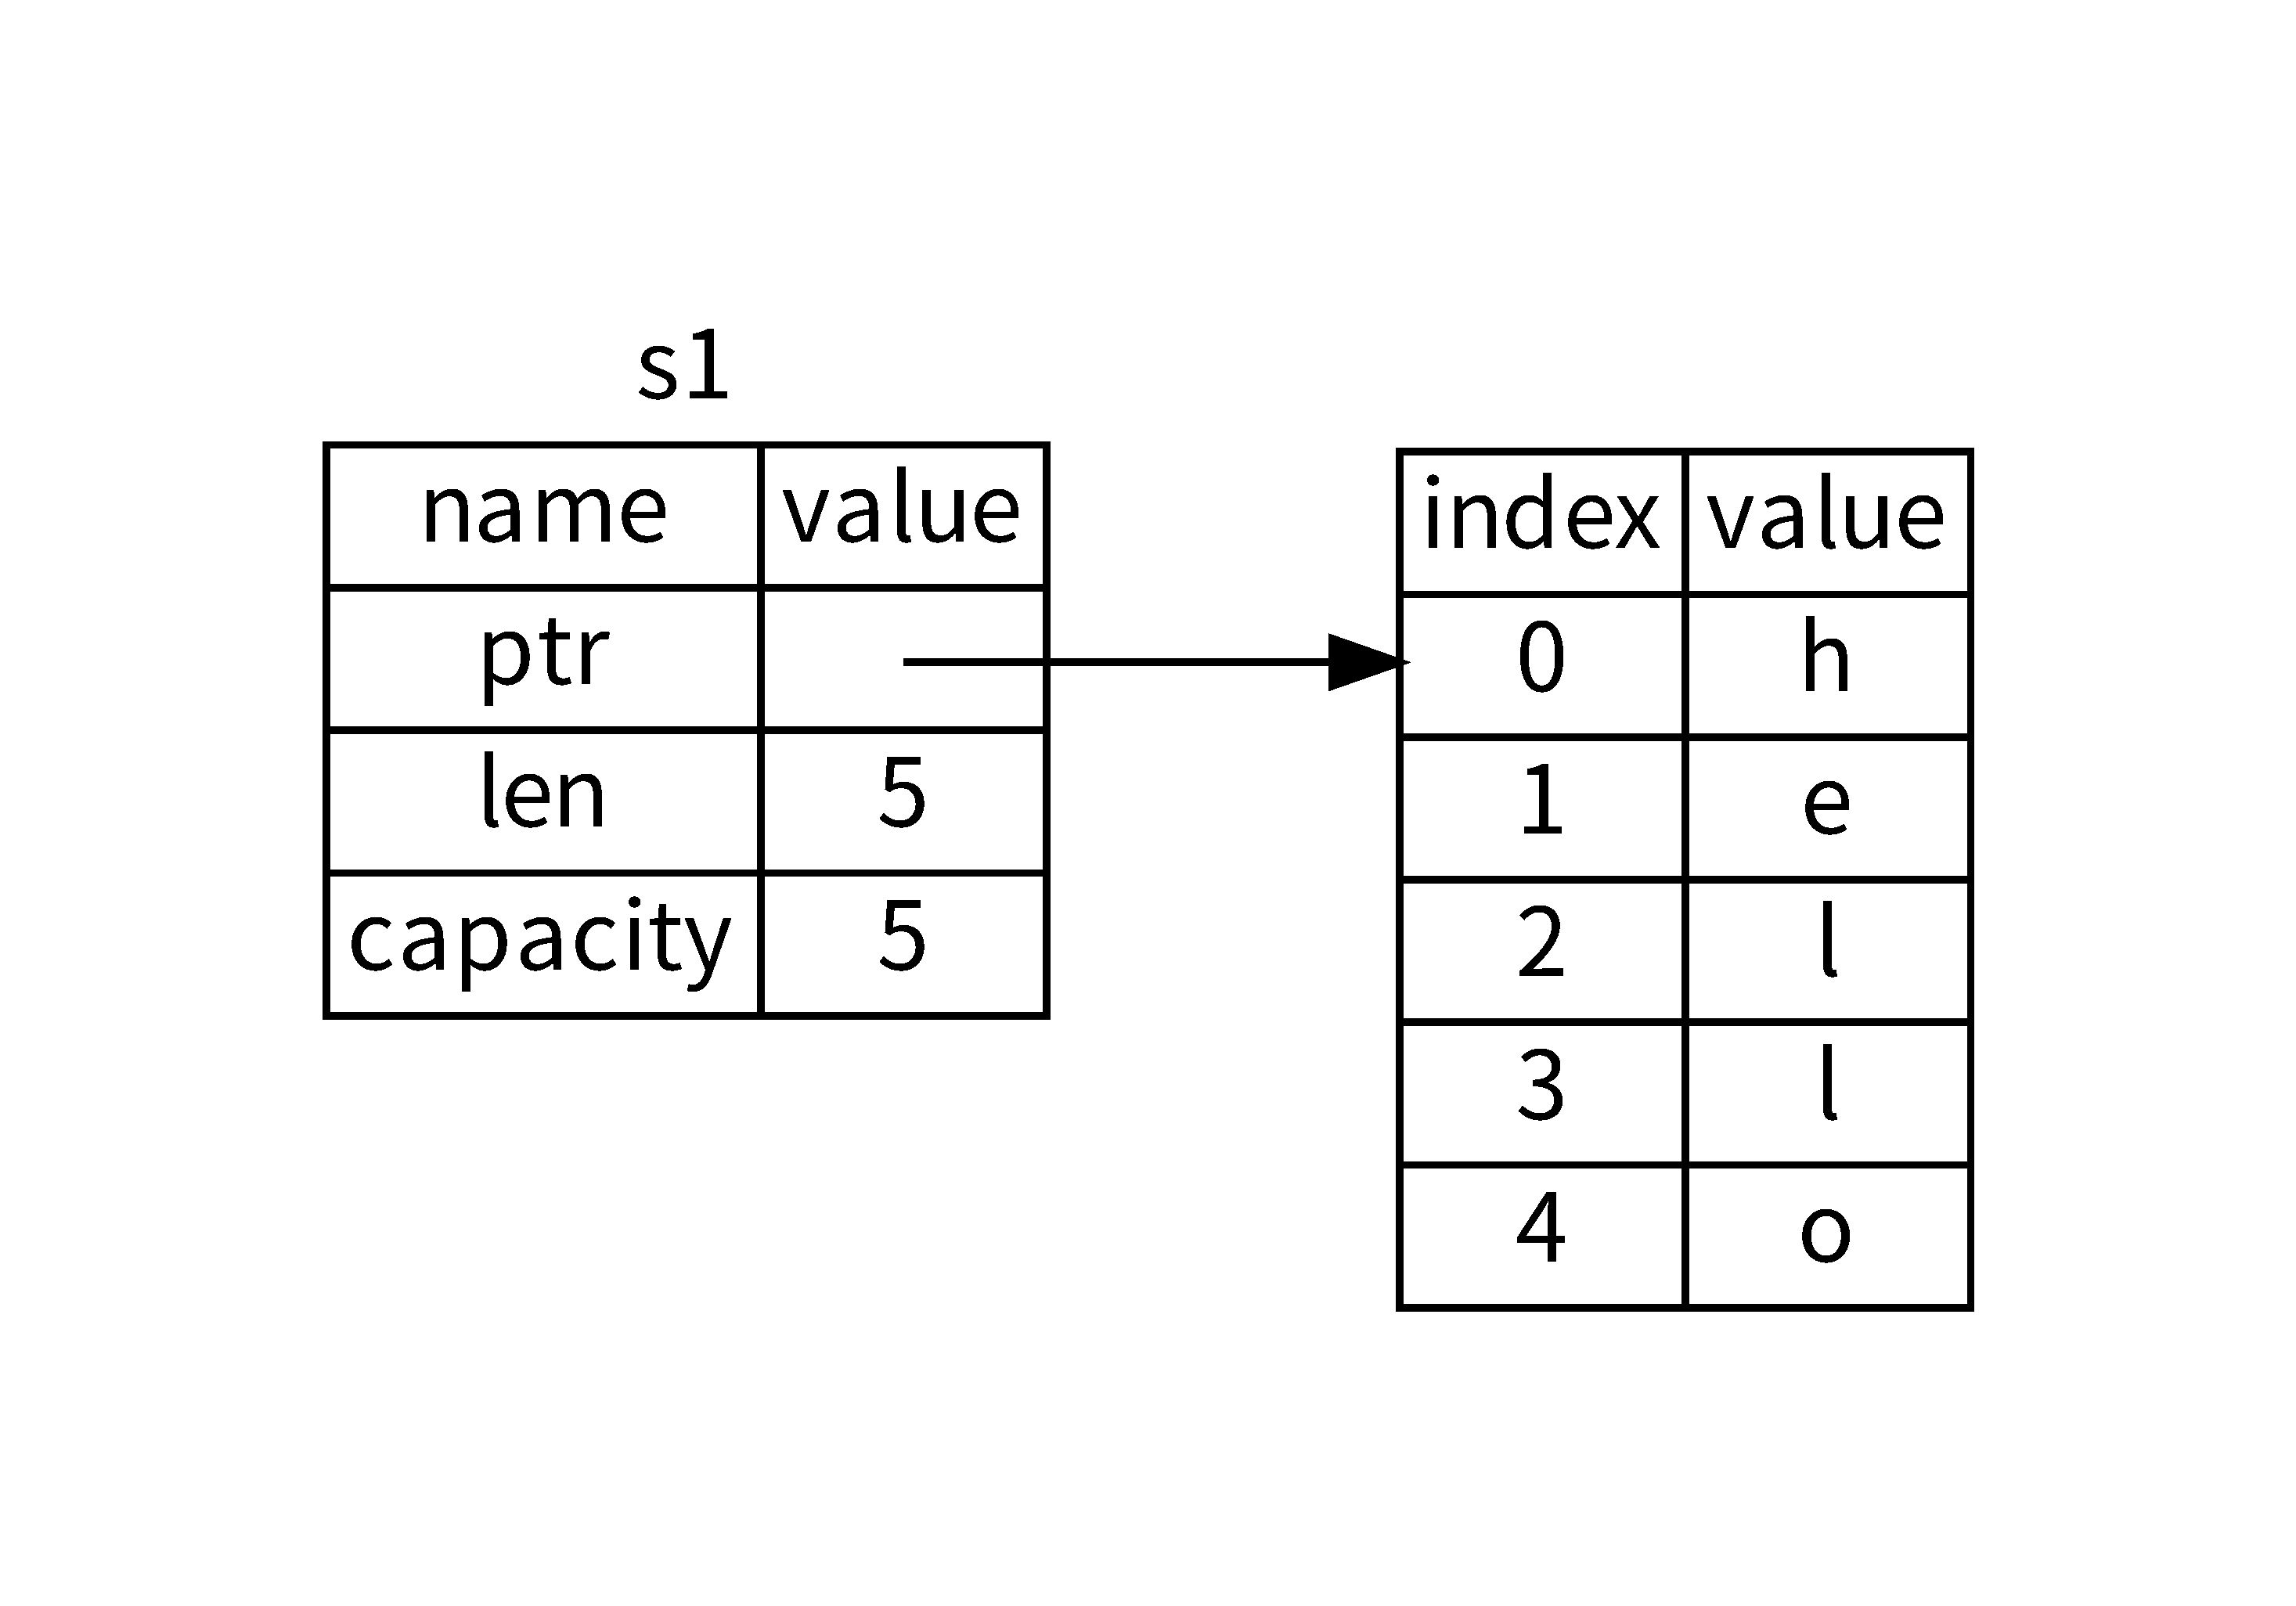
\includegraphics[width=0.5\textwidth,height=\textheight]{img/trpl04-01.pdf}

{Figure 4-1: Representation in memory of a \mintinline[]{text}{String}
holding the value \mintinline[]{text}{"hello"} bound to
\mintinline[]{text}{s1}}

The length is how much memory, in bytes, the contents of the
\mintinline[]{text}{String} is currently using. The capacity is the
total amount of memory, in bytes, that the \mintinline[]{text}{String}
has received from the operating system. The difference between length
and capacity matters, but not in this context, so for now, it's fine to
ignore the capacity.

When we assign \mintinline[]{text}{s1} to \mintinline[]{text}{s2}, the
\mintinline[]{text}{String} data is copied, meaning we copy the pointer,
the length, and the capacity that are on the stack. We do not copy the
data on the heap that the pointer refers to. In other words, the data
representation in memory looks like Figure 4-2.

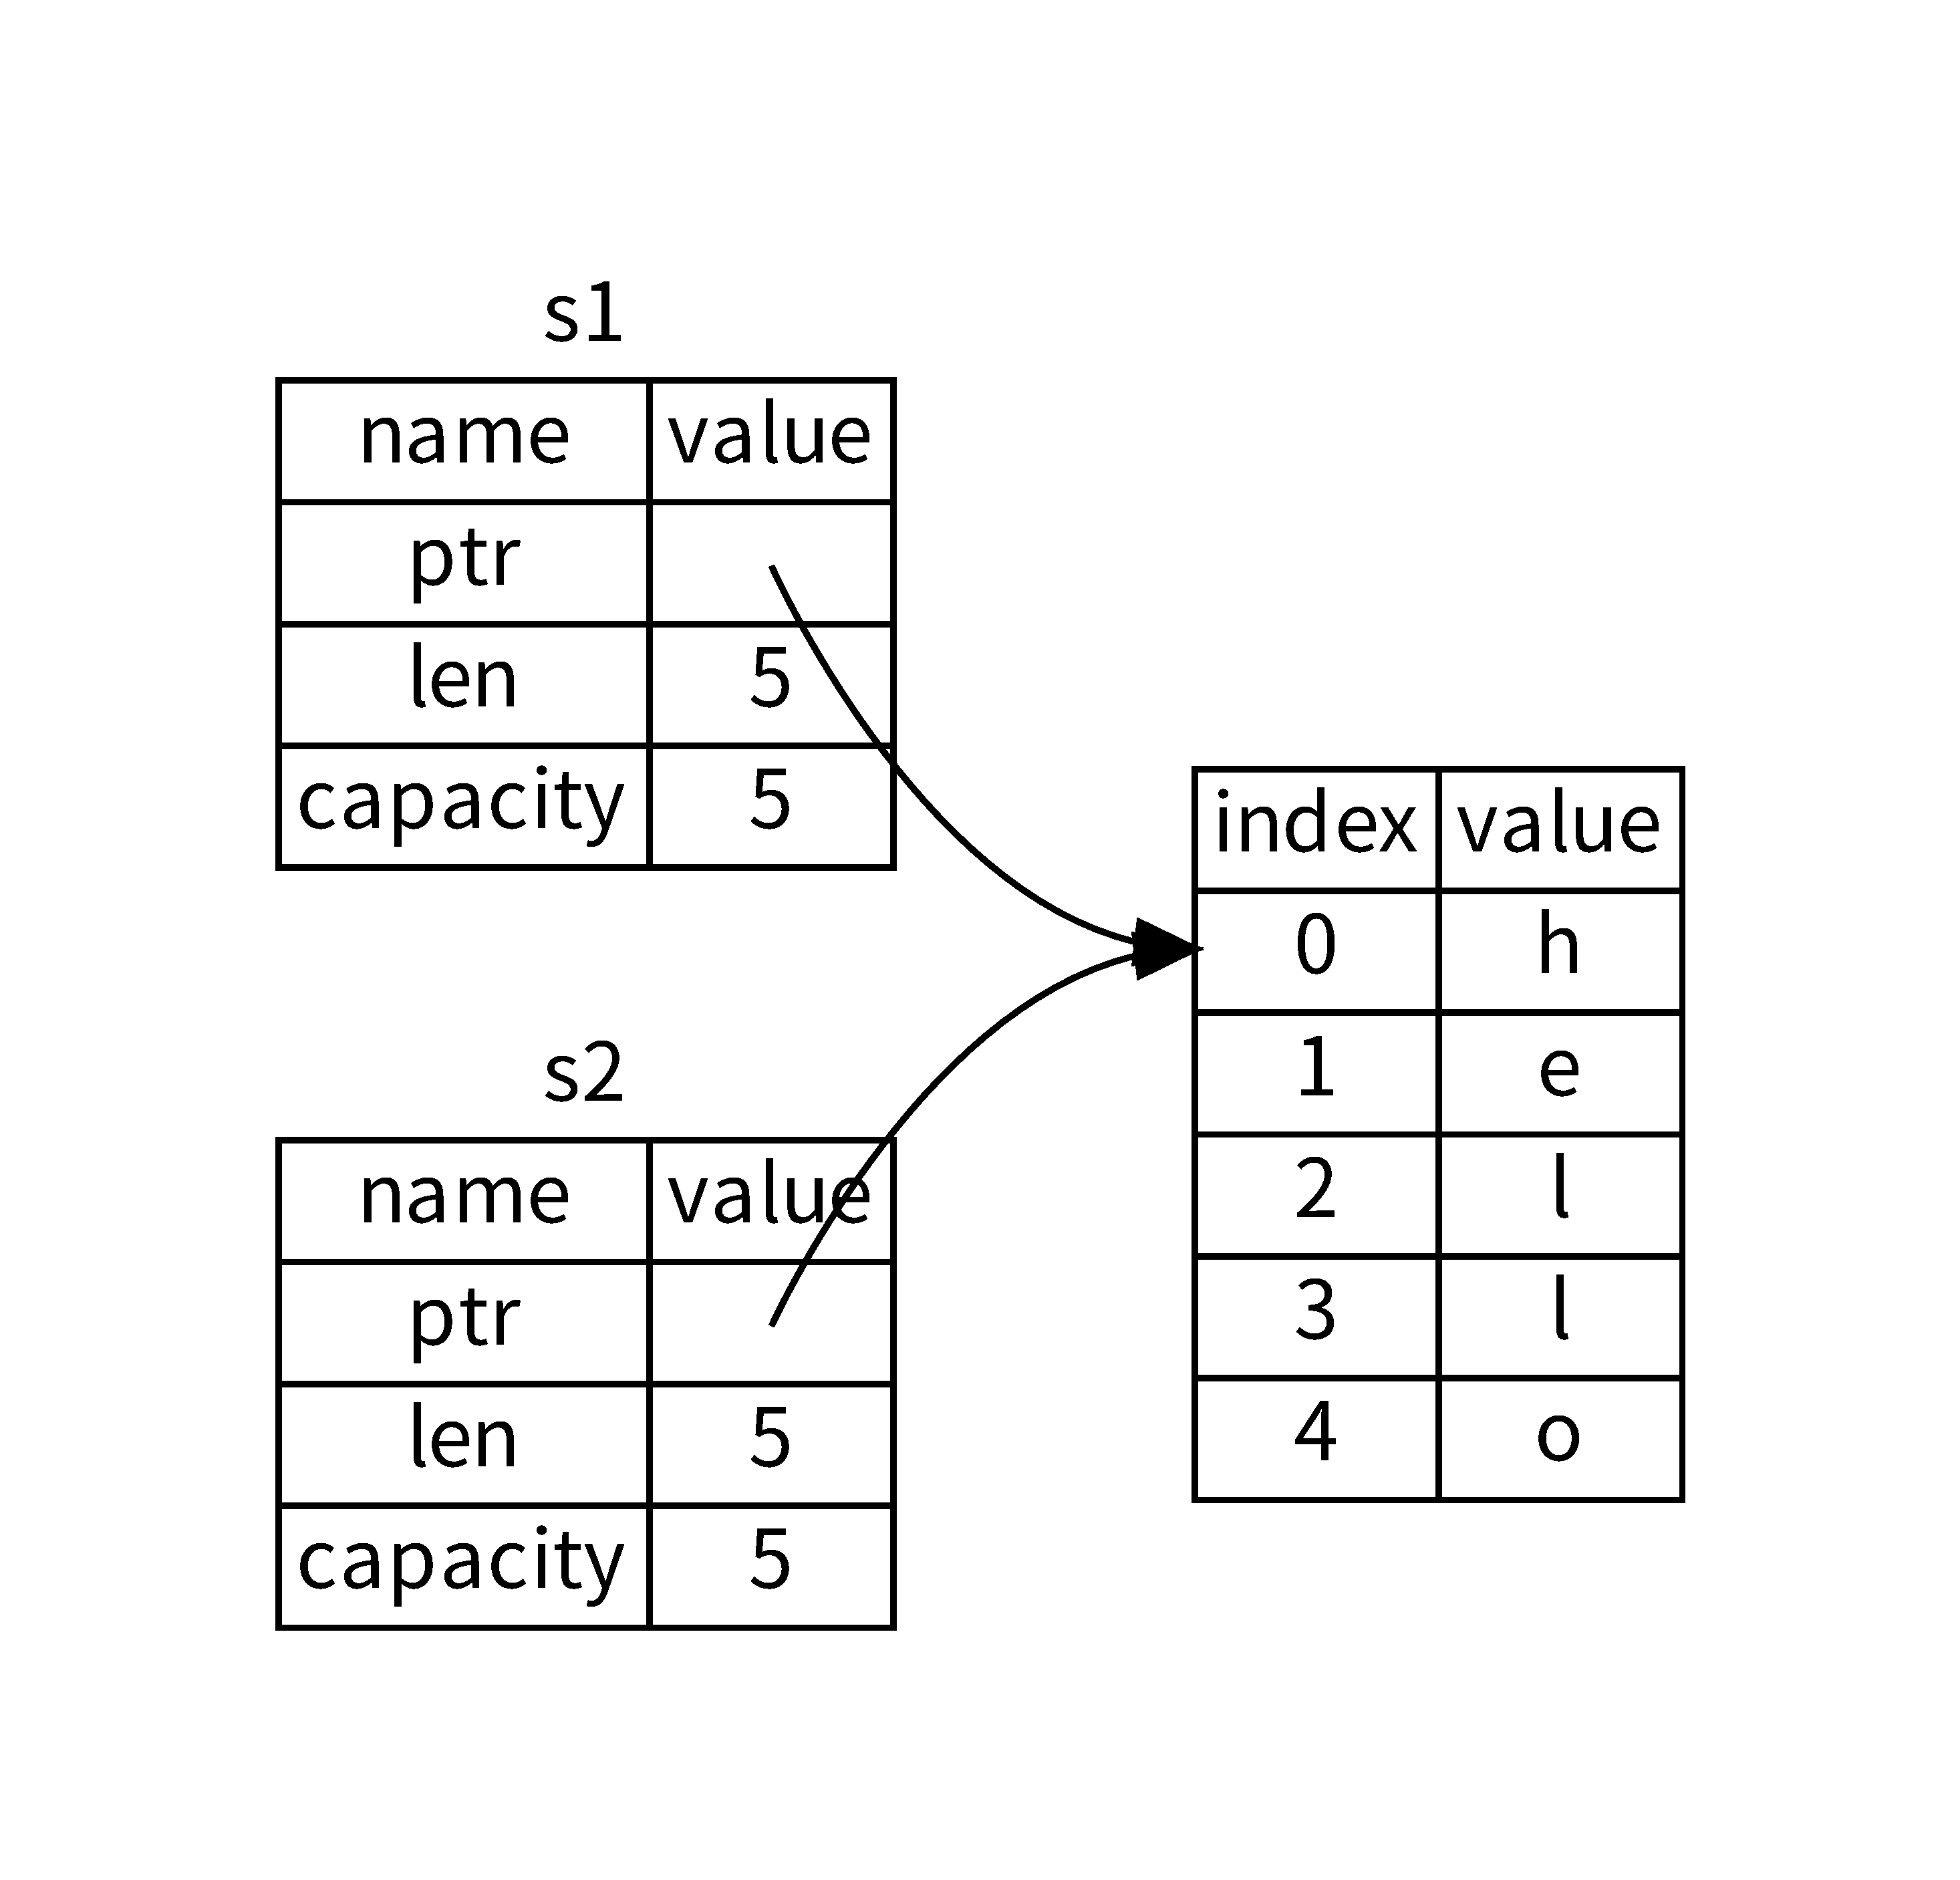
\includegraphics[width=0.5\textwidth,height=\textheight]{img/trpl04-02.pdf}

{Figure 4-2: Representation in memory of the variable
\mintinline[]{text}{s2} that has a copy of the pointer, length, and
capacity of \mintinline[]{text}{s1}}

The representation does \emph{not} look like Figure 4-3, which is what
memory would look like if Rust instead copied the heap data as well. If
Rust did this, the operation \mintinline[]{text}{s2 = s1} could be very
expensive in terms of runtime performance if the data on the heap were
large.

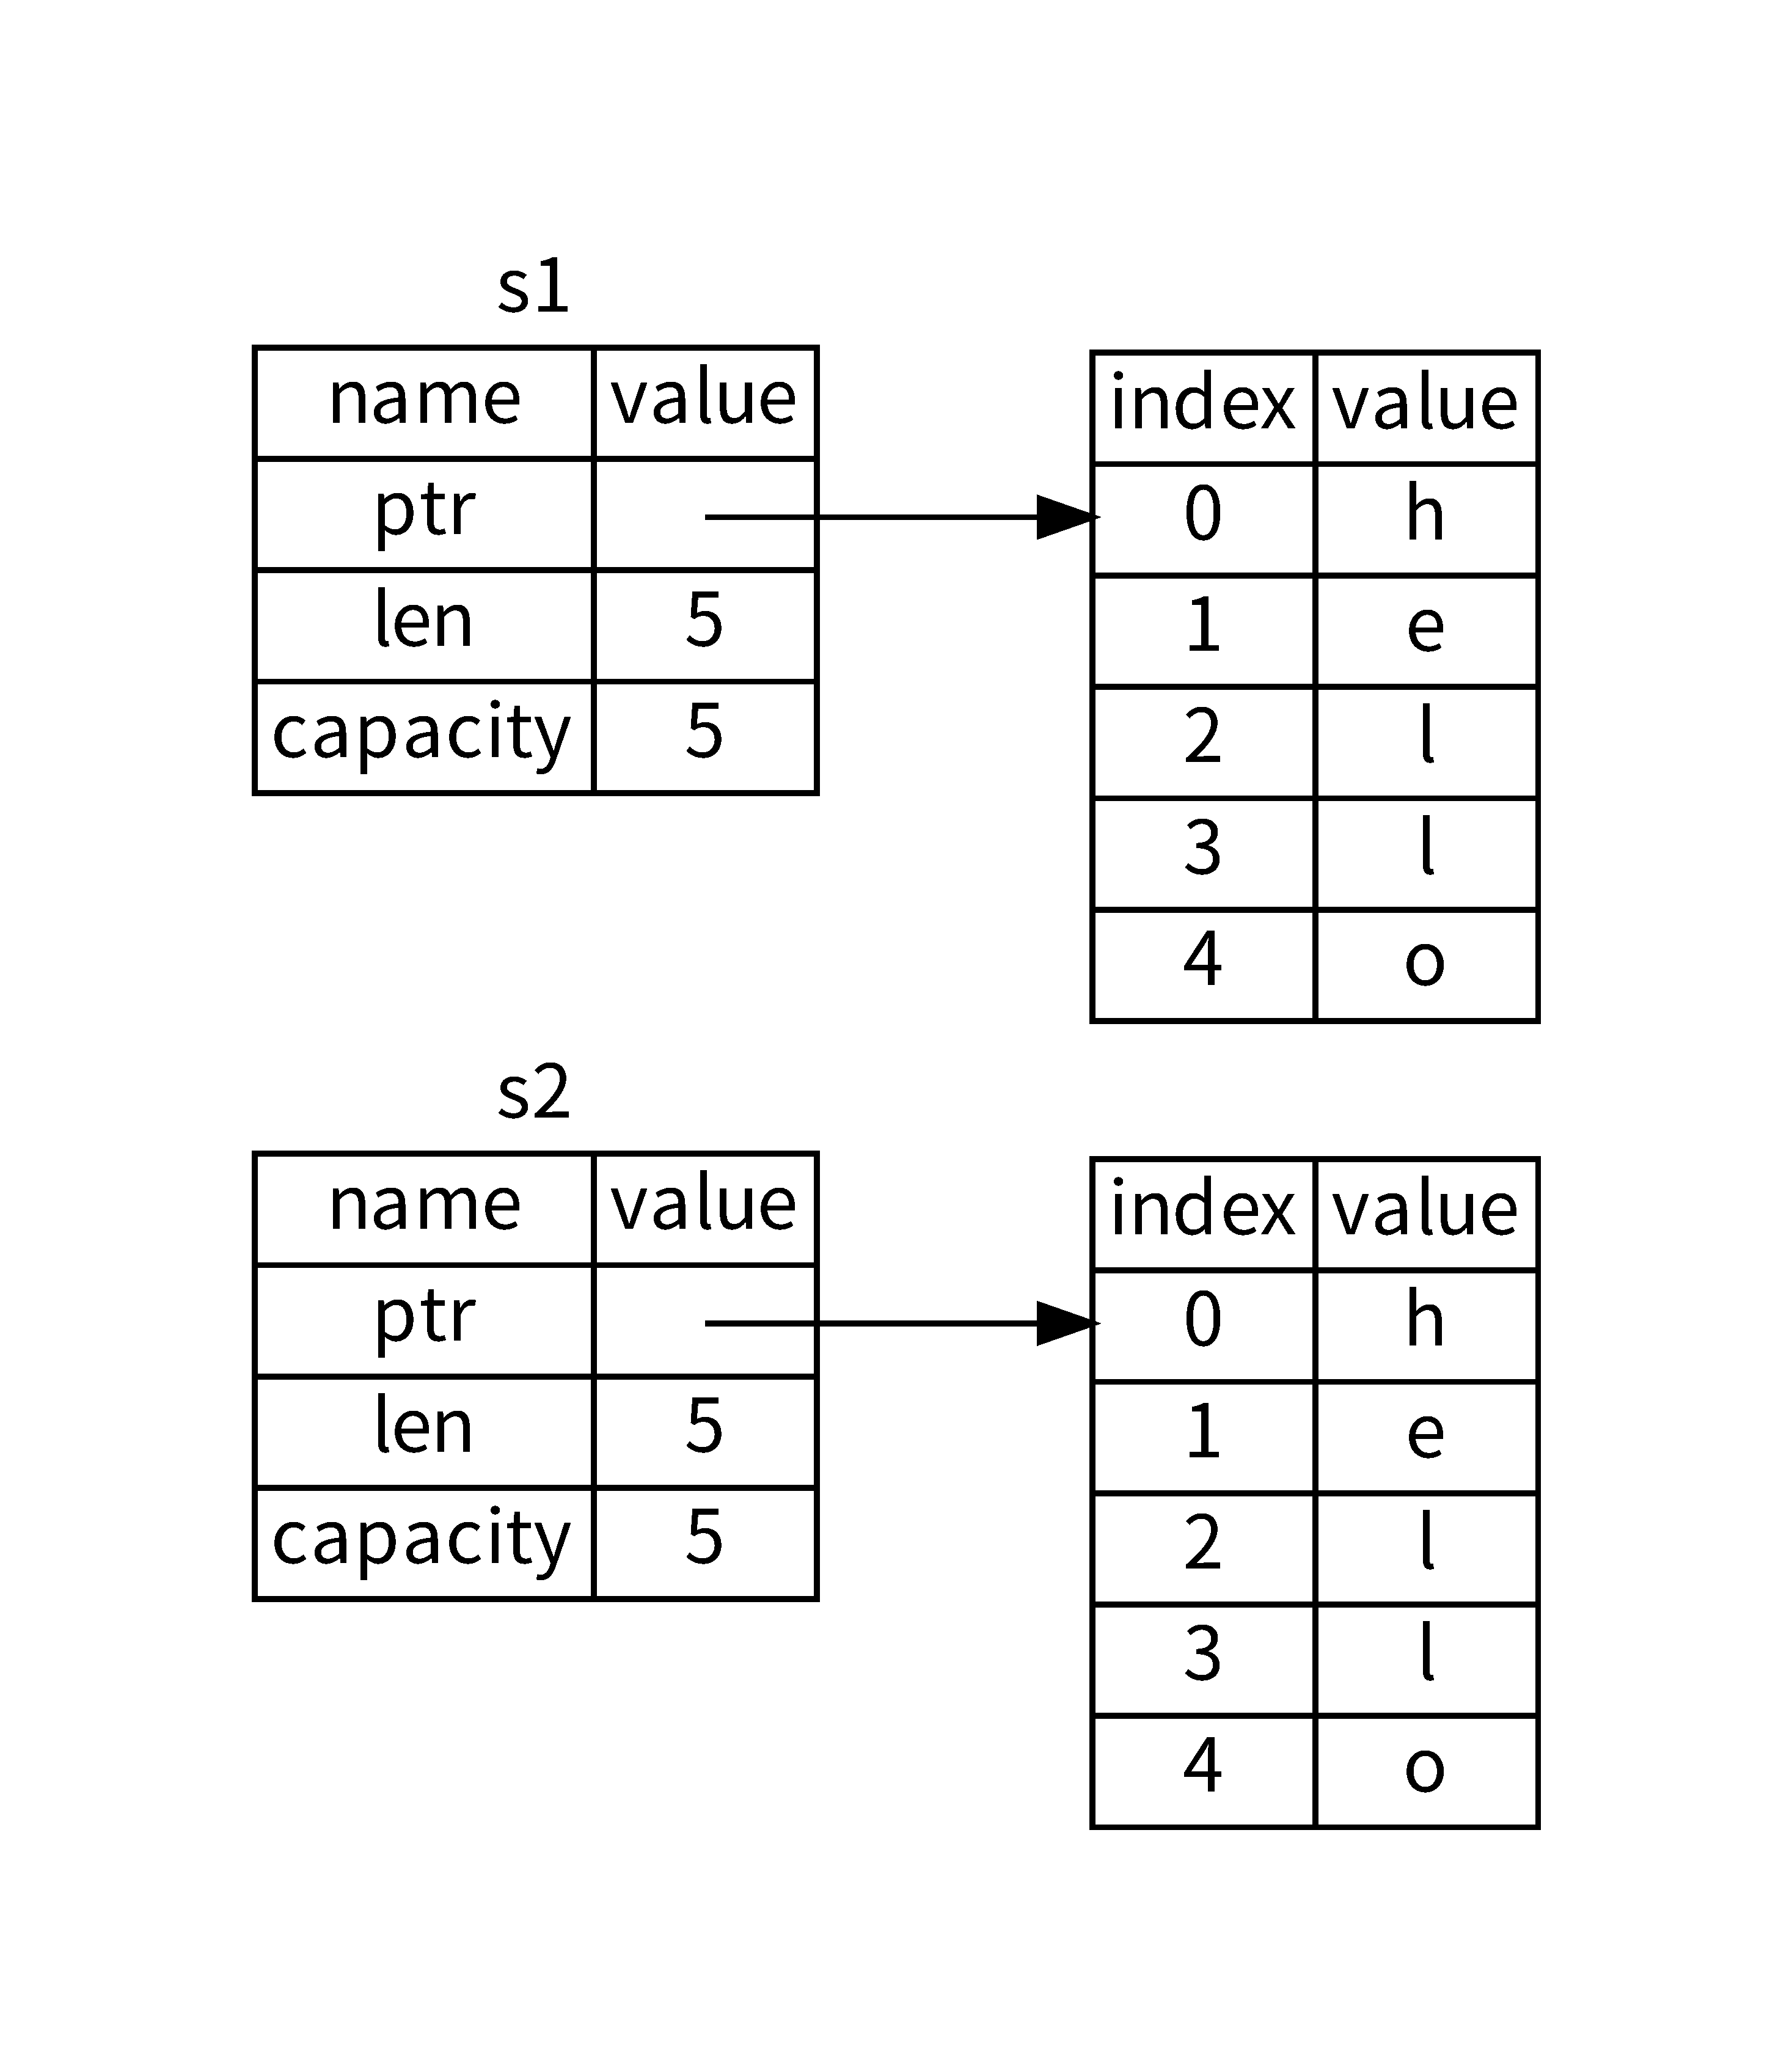
\includegraphics[width=0.5\textwidth,height=\textheight]{img/trpl04-03.pdf}

{Figure 4-3: Another possibility for what \mintinline[]{text}{s2 = s1}
might do if Rust copied the heap data as well}

Earlier, we said that when a variable goes out of scope, Rust
automatically calls the \mintinline[]{text}{drop} function and cleans up
the heap memory for that variable. But Figure 4-2 shows both data
pointers pointing to the same location. This is a problem: when
\mintinline[]{text}{s2} and \mintinline[]{text}{s1} go out of scope,
they will both try to free the same memory. This is known as a
\emph{double free} error and is one of the memory safety bugs we
mentioned previously. Freeing memory twice can lead to memory
corruption, which can potentially lead to security vulnerabilities.

To ensure memory safety, there's one more detail to what happens in this
situation in Rust. Instead of trying to copy the allocated memory, Rust
considers \mintinline[]{text}{s1} to no longer be valid and, therefore,
Rust doesn't need to free anything when \mintinline[]{text}{s1} goes out
of scope. Check out what happens when you try to use
\mintinline[]{text}{s1} after \mintinline[]{text}{s2} is created; it
won't work:

\begin{minted}[]{rust}
let s1 = String::from("hello");
let s2 = s1;

println!("{}, world!", s1);
\end{minted}

You'll get an error like this because Rust prevents you from using the
invalidated reference:

\begin{minted}[]{text}
error[E0382]: use of moved value: `s1`
 --> src/main.rs:5:28
  |
3 |     let s2 = s1;
  |         -- value moved here
4 |
5 |     println!("{}, world!", s1);
  |                            ^^ value used here after move
  |
  = note: move occurs because `s1` has type `std::string::String`, which does
  not implement the `Copy` trait
\end{minted}

If you've heard the terms \emph{shallow copy} and \emph{deep copy} while
working with other languages, the concept of copying the pointer,
length, and capacity without copying the data probably sounds like
making a shallow copy. But because Rust also invalidates the first
variable, instead of being called a shallow copy, it's known as a
\emph{move}. In this example, we would say that \mintinline[]{text}{s1}
was \emph{moved} into \mintinline[]{text}{s2}. So what actually happens
is shown in Figure 4-4.

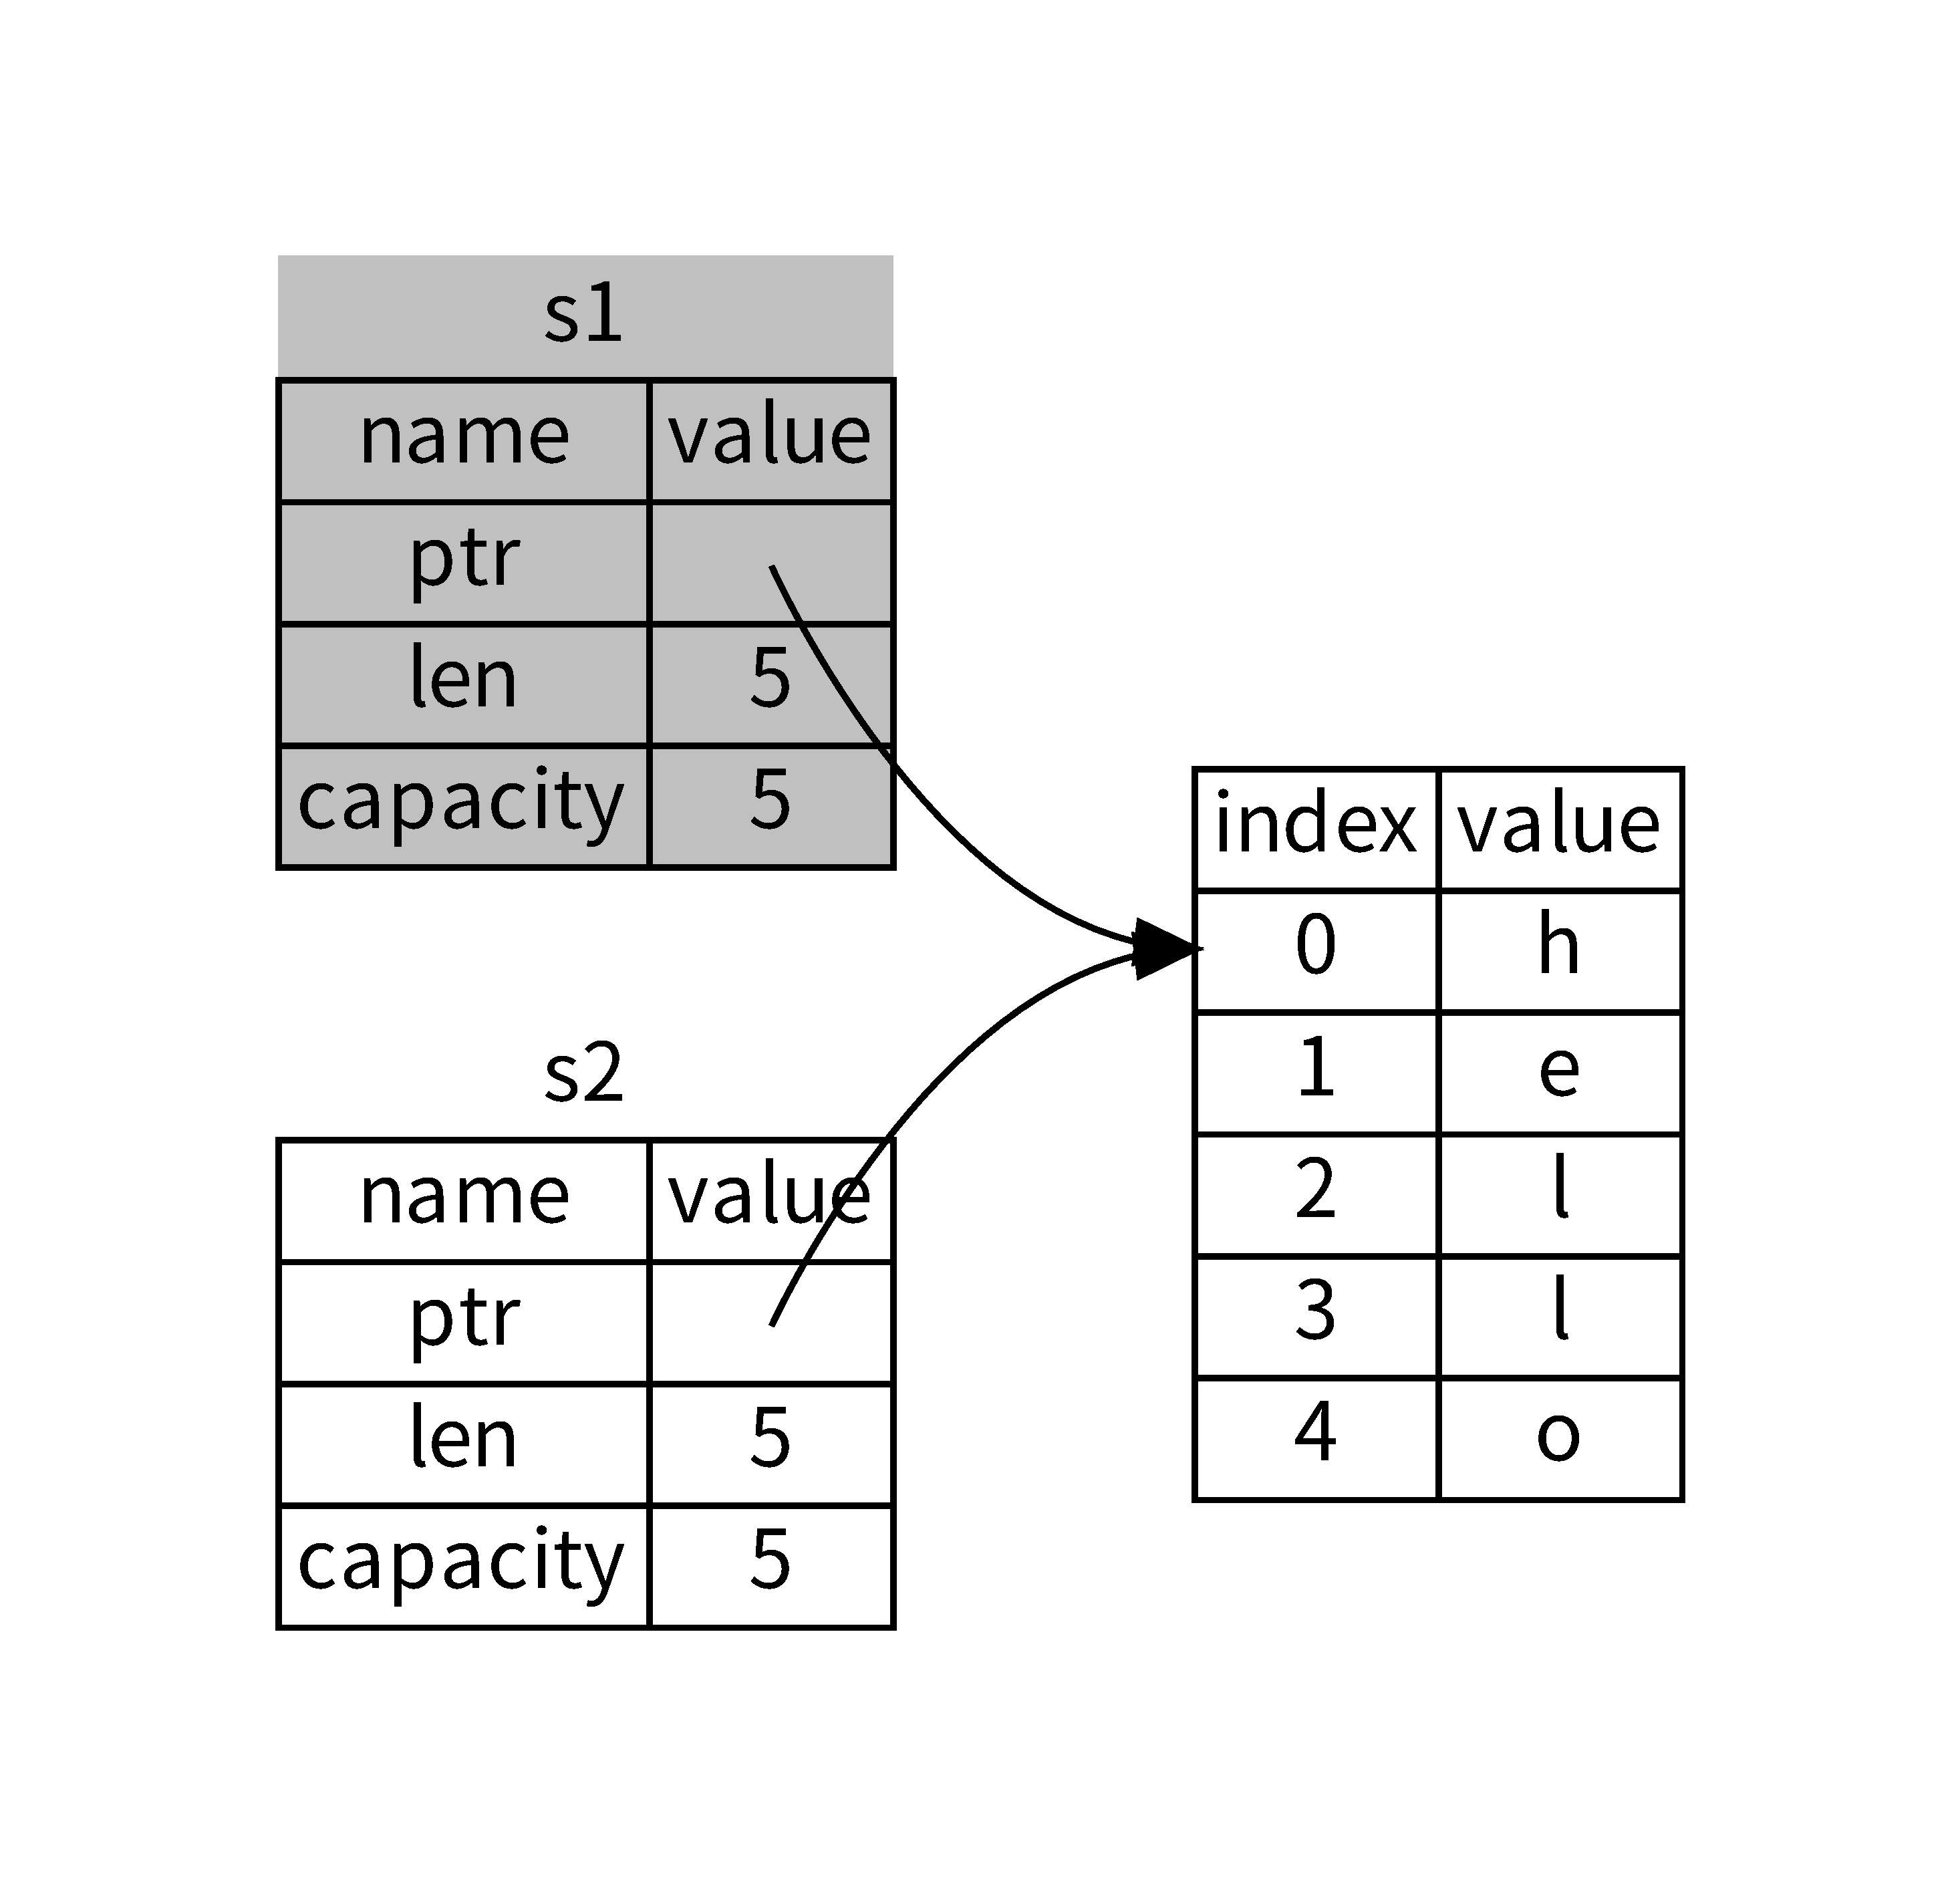
\includegraphics[width=0.5\textwidth,height=\textheight]{img/trpl04-04.pdf}

{Figure 4-4: Representation in memory after \mintinline[]{text}{s1} has
been invalidated}

That solves our problem! With only \mintinline[]{text}{s2} valid, when
it goes out of scope, it alone will free the memory, and we're done.

In addition, there's a design choice that's implied by this: Rust will
never automatically create ``deep'' copies of your data. Therefore, any
\emph{automatic} copying can be assumed to be inexpensive in terms of
runtime performance.

\hypertarget{ways-variables-and-data-interact-clone}{%
\paragraph{Ways Variables and Data Interact:
Clone}\label{ways-variables-and-data-interact-clone}}

If we \emph{do} want to deeply copy the heap data of the
\mintinline[]{text}{String}, not just the stack data, we can use a
common method called \mintinline[]{text}{clone}. We'll discuss method
syntax in Chapter 5, but because methods are a common feature in many
programming languages, you've probably seen them before.

Here's an example of the \mintinline[]{text}{clone} method in action:

\begin{minted}[]{rust}
let s1 = String::from("hello");
let s2 = s1.clone();

println!("s1 = {}, s2 = {}", s1, s2);
\end{minted}

This works just fine and explicitly produces the behavior shown in
Figure 4-3, where the heap data \emph{does} get copied.

When you see a call to \mintinline[]{text}{clone}, you know that some
arbitrary code is being executed and that code may be expensive. It's a
visual indicator that something different is going on.

\hypertarget{stack-only-data-copy}{%
\paragraph{Stack-Only Data: Copy}\label{stack-only-data-copy}}

There's another wrinkle we haven't talked about yet. This code using
integers, part of which was shown in Listing 4-2, works and is valid:

\begin{minted}[]{rust}
let x = 5;
let y = x;

println!("x = {}, y = {}", x, y);
\end{minted}

But this code seems to contradict what we just learned: we don't have a
call to \mintinline[]{text}{clone}, but \mintinline[]{text}{x} is still
valid and wasn't moved into \mintinline[]{text}{y}.

The reason is that types such as integers that have a known size at
compile time are stored entirely on the stack, so copies of the actual
values are quick to make. That means there's no reason we would want to
prevent \mintinline[]{text}{x} from being valid after we create the
variable \mintinline[]{text}{y}. In other words, there's no difference
between deep and shallow copying here, so calling
\mintinline[]{text}{clone} wouldn't do anything different from the usual
shallow copying and we can leave it out.

Rust has a special annotation called the \mintinline[]{text}{Copy} trait
that we can place on types like integers that are stored on the stack
(we'll talk more about traits in Chapter 10). If a type has the
\mintinline[]{text}{Copy} trait, an older variable is still usable after
assignment. Rust won't let us annotate a type with the
\mintinline[]{text}{Copy} trait if the type, or any of its parts, has
implemented the \mintinline[]{text}{Drop} trait. If the type needs
something special to happen when the value goes out of scope and we add
the \mintinline[]{text}{Copy} annotation to that type, we'll get a
compile-time error. To learn about how to add the
\mintinline[]{text}{Copy} annotation to your type, see
\href{appendix-03-derivable-traits.html}{``Derivable Traits''} in
Appendix C.

So what types are \mintinline[]{text}{Copy}? You can check the
documentation for the given type to be sure, but as a general rule, any
group of simple scalar values can be \mintinline[]{text}{Copy}, and
nothing that requires allocation or is some form of resource is
\mintinline[]{text}{Copy}. Here are some of the types that are
\mintinline[]{text}{Copy}:

\begin{itemize}
\tightlist
\item
  All the integer types, such as \mintinline[]{text}{u32}.
\item
  The Boolean type, \mintinline[]{text}{bool}, with values
  \mintinline[]{text}{true} and \mintinline[]{text}{false}.
\item
  All the floating point types, such as \mintinline[]{text}{f64}.
\item
  The character type, \mintinline[]{text}{char}.
\item
  Tuples, if they only contain types that are also
  \mintinline[]{text}{Copy}. For example,
  \mintinline[]{text}{(i32, i32)} is \mintinline[]{text}{Copy}, but
  \mintinline[]{text}{(i32, String)} is not.
\end{itemize}

\hypertarget{ownership-and-functions}{%
\subsubsection{Ownership and Functions}\label{ownership-and-functions}}

The semantics for passing a value to a function are similar to those for
assigning a value to a variable. Passing a variable to a function will
move or copy, just as assignment does. Listing 4-3 has an example with
some annotations showing where variables go into and out of scope.

{Filename: src/main.rs}

\begin{minted}[]{rust}
fn main() {
    let s = String::from("hello");  // s comes into scope

    takes_ownership(s);             // s's value moves into the function...
                                    // ... and so is no longer valid here

    let x = 5;                      // x comes into scope

    makes_copy(x);                  // x would move into the function,
                                    // but i32 is Copy, so it’s okay to still
                                    // use x afterward

} // Here, x goes out of scope, then s. But because s's value was moved, nothing
  // special happens.

fn takes_ownership(some_string: String) { // some_string comes into scope
    println!("{}", some_string);
} // Here, some_string goes out of scope and `drop` is called. The backing
  // memory is freed.

fn makes_copy(some_integer: i32) { // some_integer comes into scope
    println!("{}", some_integer);
} // Here, some_integer goes out of scope. Nothing special happens.
\end{minted}

{Listing 4-3: Functions with ownership and scope annotated}

If we tried to use \mintinline[]{text}{s} after the call to
\mintinline[]{text}{takes_ownership}, Rust would throw a compile-time
error. These static checks protect us from mistakes. Try adding code to
\mintinline[]{text}{main} that uses \mintinline[]{text}{s} and
\mintinline[]{text}{x} to see where you can use them and where the
ownership rules prevent you from doing so.

\hypertarget{return-values-and-scope}{%
\subsubsection{Return Values and Scope}\label{return-values-and-scope}}

Returning values can also transfer ownership. Listing 4-4 is an example
with similar annotations to those in Listing 4-3.

{Filename: src/main.rs}

\begin{minted}[]{rust}
fn main() {
    let s1 = gives_ownership();         // gives_ownership moves its return
                                        // value into s1

    let s2 = String::from("hello");     // s2 comes into scope

    let s3 = takes_and_gives_back(s2);  // s2 is moved into
                                        // takes_and_gives_back, which also
                                        // moves its return value into s3
} // Here, s3 goes out of scope and is dropped. s2 goes out of scope but was
  // moved, so nothing happens. s1 goes out of scope and is dropped.

fn gives_ownership() -> String {             // gives_ownership will move its
                                             // return value into the function
                                             // that calls it

    let some_string = String::from("hello"); // some_string comes into scope

    some_string                              // some_string is returned and
                                             // moves out to the calling
                                             // function
}

// takes_and_gives_back will take a String and return one
fn takes_and_gives_back(a_string: String) -> String { // a_string comes into
                                                      // scope

    a_string  // a_string is returned and moves out to the calling function
}
\end{minted}

{Listing 4-4: Transferring ownership of return values}

The ownership of a variable follows the same pattern every time:
assigning a value to another variable moves it. When a variable that
includes data on the heap goes out of scope, the value will be cleaned
up by \mintinline[]{text}{drop} unless the data has been moved to be
owned by another variable.

Taking ownership and then returning ownership with every function is a
bit tedious. What if we want to let a function use a value but not take
ownership? It's quite annoying that anything we pass in also needs to be
passed back if we want to use it again, in addition to any data
resulting from the body of the function that we might want to return as
well.

It's possible to return multiple values using a tuple, as shown in
Listing 4-5.

{Filename: src/main.rs}

\begin{minted}[]{rust}
fn main() {
    let s1 = String::from("hello");

    let (s2, len) = calculate_length(s1);

    println!("The length of '{}' is {}.", s2, len);
}

fn calculate_length(s: String) -> (String, usize) {
    let length = s.len(); // len() returns the length of a String

    (s, length)
}
\end{minted}

{Listing 4-5: Returning ownership of parameters}

But this is too much ceremony and a lot of work for a concept that
should be common. Luckily for us, Rust has a feature for this concept,
called \emph{references}.

\hypertarget{references-and-borrowing}{%
\subsection{References and Borrowing}\label{references-and-borrowing}}

The issue with the tuple code in Listing 4-5 is that we have to return
the \mintinline[]{text}{String} to the calling function so we can still
use the \mintinline[]{text}{String} after the call to
\mintinline[]{text}{calculate_length}, because the
\mintinline[]{text}{String} was moved into
\mintinline[]{text}{calculate_length}.

Here is how you would define and use a
\mintinline[]{text}{calculate_length} function that has a reference to
an object as a parameter instead of taking ownership of the value:

{Filename: src/main.rs}

\begin{minted}[]{rust}
fn main() {
    let s1 = String::from("hello");

    let len = calculate_length(&s1);

    println!("The length of '{}' is {}.", s1, len);
}

fn calculate_length(s: &String) -> usize {
    s.len()
}
\end{minted}

First, notice that all the tuple code in the variable declaration and
the function return value is gone. Second, note that we pass
\mintinline[]{text}{&s1} into \mintinline[]{text}{calculate_length} and,
in its definition, we take \mintinline[]{text}{&String} rather than
\mintinline[]{text}{String}.

These ampersands are \emph{references}, and they allow you to refer to
some value without taking ownership of it. Figure 4-5 shows a diagram.

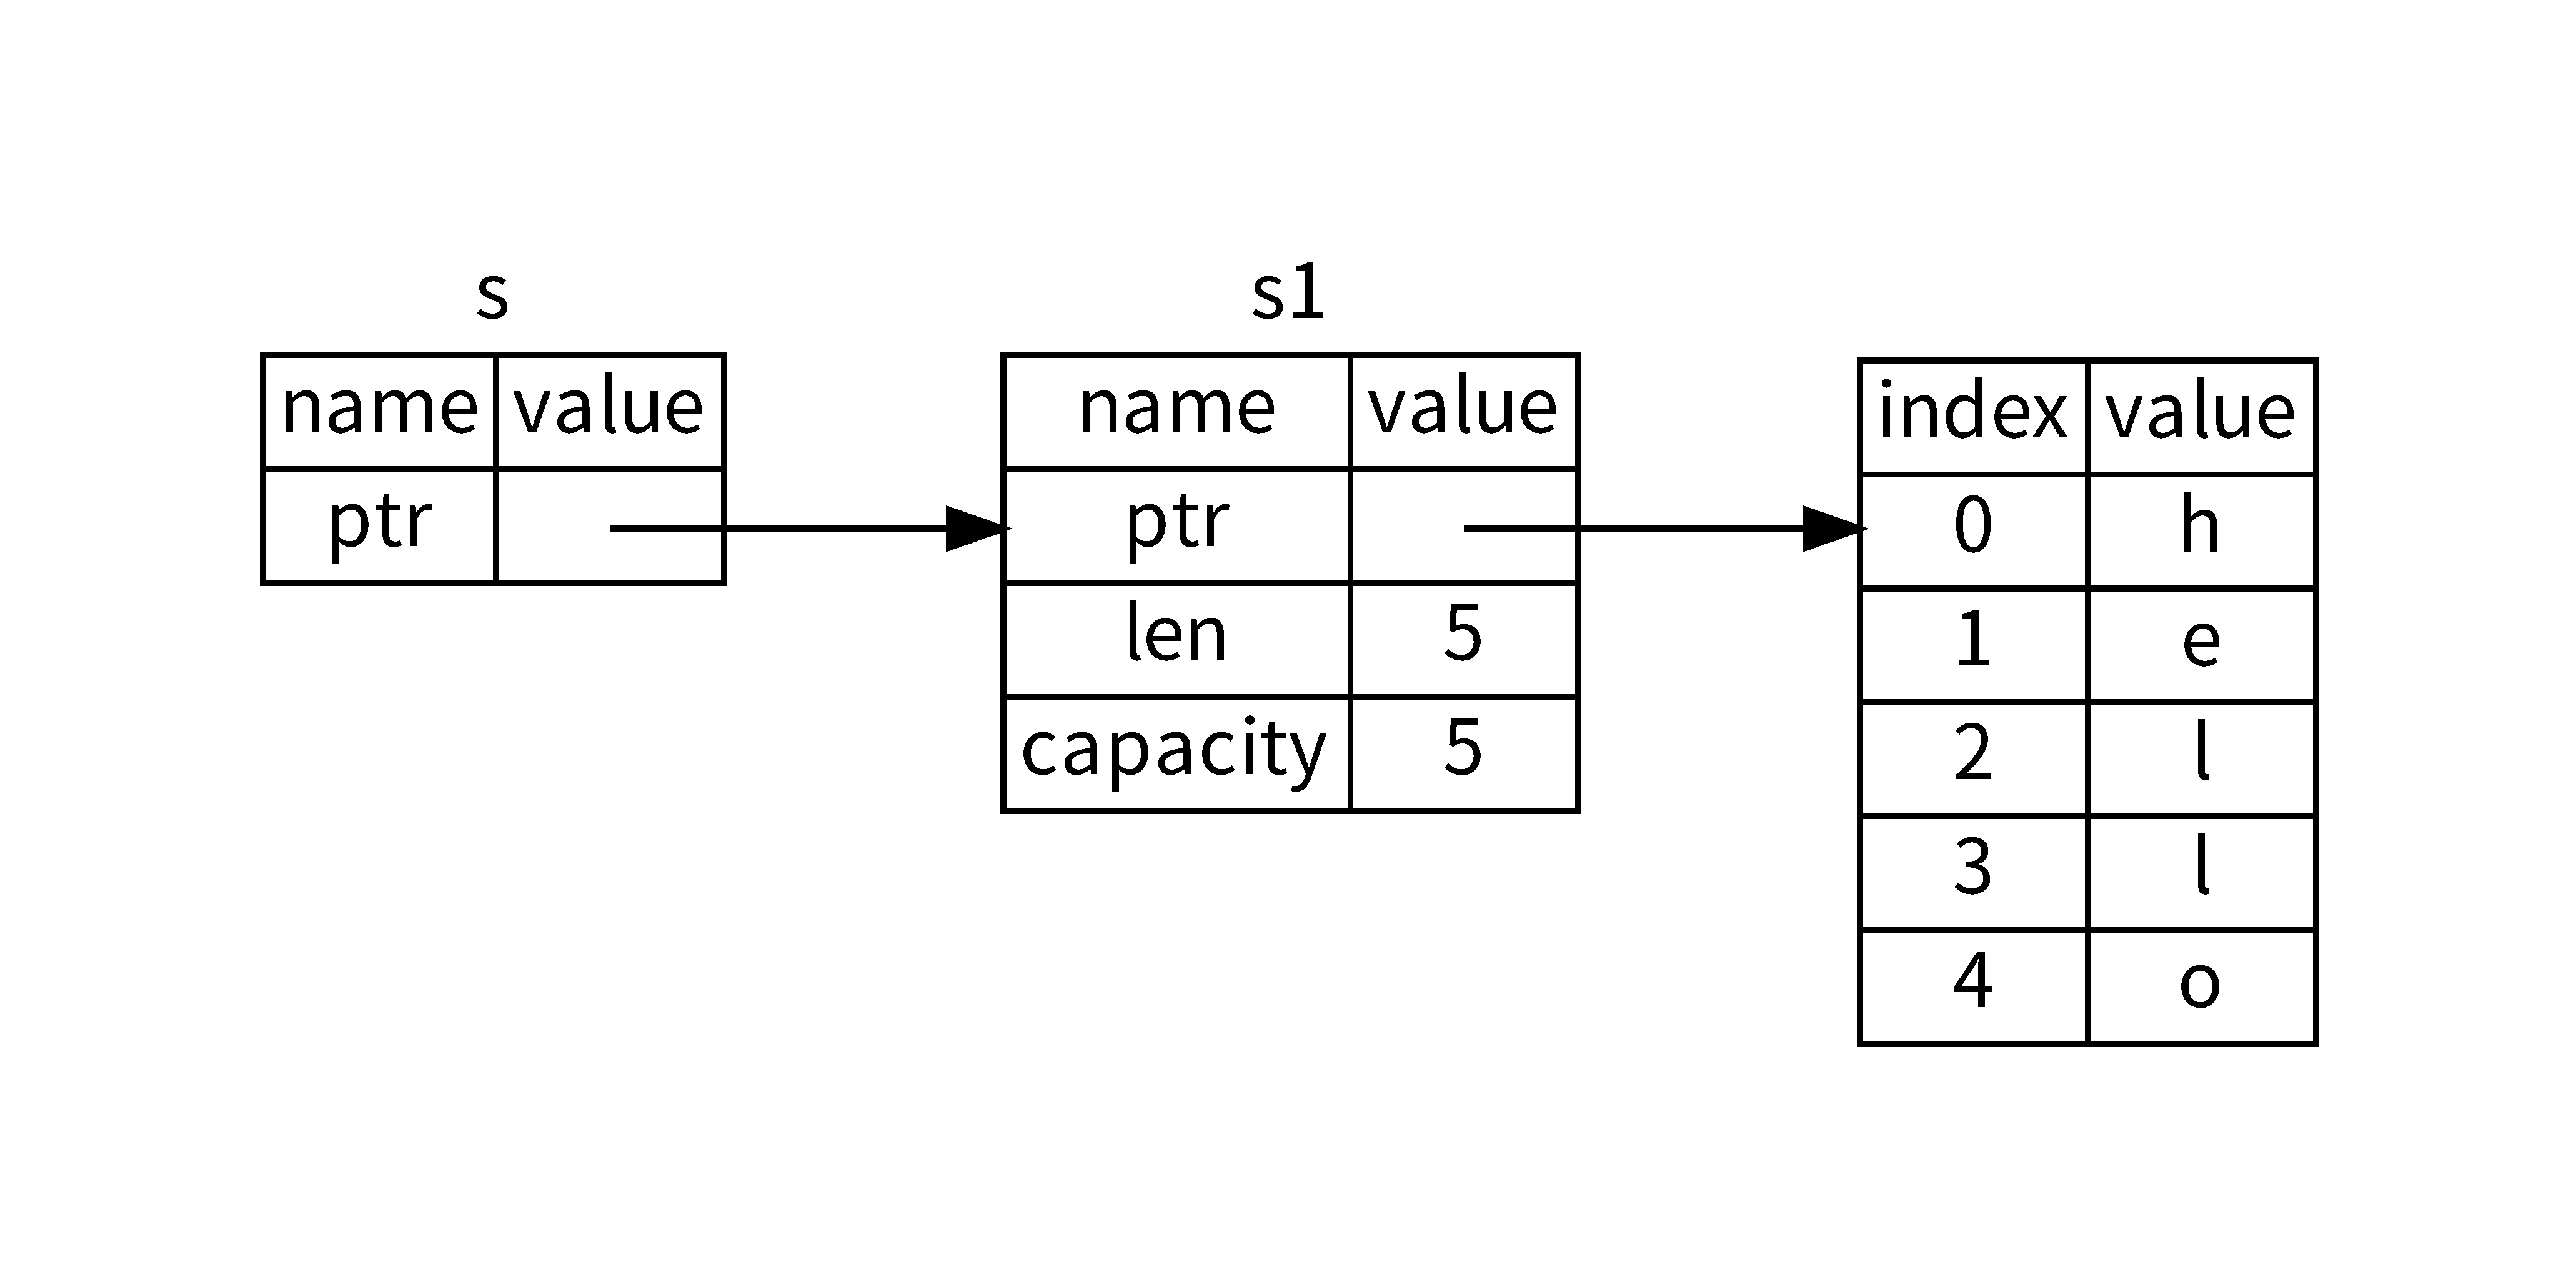
\includegraphics{img/trpl04-05.pdf}

{Figure 4-5: A diagram of \mintinline[]{text}{&String s} pointing at
\mintinline[]{text}{String s1}}

\begin{quote}
Note: The opposite of referencing by using \mintinline[]{text}{&} is
\emph{dereferencing}, which is accomplished with the dereference
operator, \mintinline[]{text}{*}. We'll see some uses of the dereference
operator in Chapter 8 and discuss details of dereferencing in Chapter
15.
\end{quote}

Let's take a closer look at the function call here:

\begin{minted}[]{rust}
# fn calculate_length(s: &String) -> usize {
#     s.len()
# }
let s1 = String::from("hello");

let len = calculate_length(&s1);
\end{minted}

The \mintinline[]{text}{&s1} syntax lets us create a reference that
\emph{refers} to the value of \mintinline[]{text}{s1} but does not own
it. Because it does not own it, the value it points to will not be
dropped when the reference goes out of scope.

Likewise, the signature of the function uses \mintinline[]{text}{&} to
indicate that the type of the parameter \mintinline[]{text}{s} is a
reference. Let's add some explanatory annotations:

\begin{minted}[]{rust}
fn calculate_length(s: &String) -> usize { // s is a reference to a String
    s.len()
} // Here, s goes out of scope. But because it does not have ownership of what
  // it refers to, nothing happens.
\end{minted}

The scope in which the variable \mintinline[]{text}{s} is valid is the
same as any function parameter's scope, but we don't drop what the
reference points to when it goes out of scope because we don't have
ownership. When functions have references as parameters instead of the
actual values, we won't need to return the values in order to give back
ownership, because we never had ownership.

We call having references as function parameters \emph{borrowing}. As in
real life, if a person owns something, you can borrow it from them. When
you're done, you have to give it back.

So what happens if we try to modify something we're borrowing? Try the
code in Listing 4-6. Spoiler alert: it doesn't work!

{Filename: src/main.rs}

\begin{minted}[]{rust}
fn main() {
    let s = String::from("hello");

    change(&s);
}

fn change(some_string: &String) {
    some_string.push_str(", world");
}
\end{minted}

{Listing 4-6: Attempting to modify a borrowed value}

Here's the error:

\begin{minted}[]{text}
error[E0596]: cannot borrow immutable borrowed content `*some_string` as mutable
 --> error.rs:8:5
  |
7 | fn change(some_string: &String) {
  |                        ------- use `&mut String` here to make mutable
8 |     some_string.push_str(", world");
  |     ^^^^^^^^^^^ cannot borrow as mutable
\end{minted}

Just as variables are immutable by default, so are references. We're not
allowed to modify something we have a reference to.

\hypertarget{mutable-references}{%
\subsubsection{Mutable References}\label{mutable-references}}

We can fix the error in the code from Listing 4-6 with just a small
tweak:

{Filename: src/main.rs}

\begin{minted}[]{rust}
fn main() {
    let mut s = String::from("hello");

    change(&mut s);
}

fn change(some_string: &mut String) {
    some_string.push_str(", world");
}
\end{minted}

First, we had to change \mintinline[]{text}{s} to be
\mintinline[]{text}{mut}. Then we had to create a mutable reference with
\mintinline[]{text}{&mut s} and accept a mutable reference with
\mintinline[]{text}{some_string: &mut String}.

But mutable references have one big restriction: you can have only one
mutable reference to a particular piece of data in a particular scope.
This code will fail:

{Filename: src/main.rs}

\begin{minted}[]{rust}
let mut s = String::from("hello");

let r1 = &mut s;
let r2 = &mut s;

println!("{}, {}", r1, r2);
\end{minted}

Here's the error:

\begin{minted}[]{text}
error[E0499]: cannot borrow `s` as mutable more than once at a time
 --> src/main.rs:5:14
  |
4 |     let r1 = &mut s;
  |              ------ first mutable borrow occurs here
5 |     let r2 = &mut s;
  |              ^^^^^^ second mutable borrow occurs here
6 |
7 |     println!("{}, {}", r1, r2);
  |                        -- first borrow later used here
\end{minted}

This restriction allows for mutation but in a very controlled fashion.
It's something that new Rustaceans struggle with, because most languages
let you mutate whenever you'd like.

The benefit of having this restriction is that Rust can prevent data
races at compile time. A \emph{data race} is similar to a race condition
and happens when these three behaviors occur:

\begin{itemize}
\tightlist
\item
  Two or more pointers access the same data at the same time.
\item
  At least one of the pointers is being used to write to the data.
\item
  There's no mechanism being used to synchronize access to the data.
\end{itemize}

Data races cause undefined behavior and can be difficult to diagnose and
fix when you're trying to track them down at runtime; Rust prevents this
problem from happening because it won't even compile code with data
races!

As always, we can use curly brackets to create a new scope, allowing for
multiple mutable references, just not \emph{simultaneous} ones:

\begin{minted}[]{rust}
let mut s = String::from("hello");

{
    let r1 = &mut s;

} // r1 goes out of scope here, so we can make a new reference with no problems.

let r2 = &mut s;
\end{minted}

A similar rule exists for combining mutable and immutable references.
This code results in an error:

\begin{minted}[]{rust}
let mut s = String::from("hello");

let r1 = &s; // no problem
let r2 = &s; // no problem
let r3 = &mut s; // BIG PROBLEM

println!("{}, {}, and {}", r1, r2, r3);
\end{minted}

Here's the error:

\begin{minted}[]{text}
error[E0502]: cannot borrow `s` as mutable because it is also borrowed as immutable
 --> src/main.rs:6:14
  |
4 |     let r1 = &s; // no problem
  |              -- immutable borrow occurs here
5 |     let r2 = &s; // no problem
6 |     let r3 = &mut s; // BIG PROBLEM
  |              ^^^^^^ mutable borrow occurs here
7 |
8 |     println!("{}, {}, and {}", r1, r2, r3);
  |                                -- immutable borrow later used here
\end{minted}

Whew! We \emph{also} cannot have a mutable reference while we have an
immutable one. Users of an immutable reference don't expect the values
to suddenly change out from under them! However, multiple immutable
references are okay because no one who is just reading the data has the
ability to affect anyone else's reading of the data.

Note that a reference's scope starts from where it is introduced and
continues through the last time that reference is used. For instance,
this code will compile because the last usage of the immutable
references occurs before the mutable reference is introduced:

\begin{minted}[]{rust}
let mut s = String::from("hello");

let r1 = &s; // no problem
let r2 = &s; // no problem
println!("{} and {}", r1, r2);
// r1 and r2 are no longer used after this point

let r3 = &mut s; // no problem
println!("{}", r3);
\end{minted}

The scopes of the immutable references \mintinline[]{text}{r1} and
\mintinline[]{text}{r2} end after the \mintinline[]{text}{println!}
where they are last used, which is before the mutable reference
\mintinline[]{text}{r3} is created. These scopes don't overlap, so this
code is allowed.

Even though borrowing errors may be frustrating at times, remember that
it's the Rust compiler pointing out a potential bug early (at compile
time rather than at runtime) and showing you exactly where the problem
is. Then you don't have to track down why your data isn't what you
thought it was.

\hypertarget{dangling-references}{%
\subsubsection{Dangling References}\label{dangling-references}}

In languages with pointers, it's easy to erroneously create a
\emph{dangling pointer}, a pointer that references a location in memory
that may have been given to someone else, by freeing some memory while
preserving a pointer to that memory. In Rust, by contrast, the compiler
guarantees that references will never be dangling references: if you
have a reference to some data, the compiler will ensure that the data
will not go out of scope before the reference to the data does.

Let's try to create a dangling reference, which Rust will prevent with a
compile-time error:

{Filename: src/main.rs}

\begin{minted}[]{rust}
fn main() {
    let reference_to_nothing = dangle();
}

fn dangle() -> &String {
    let s = String::from("hello");

    &s
}
\end{minted}

Here's the error:

\begin{minted}[]{text}
error[E0106]: missing lifetime specifier
 --> main.rs:5:16
  |
5 | fn dangle() -> &String {
  |                ^ expected lifetime parameter
  |
  = help: this function's return type contains a borrowed value, but there is
  no value for it to be borrowed from
  = help: consider giving it a 'static lifetime
\end{minted}

This error message refers to a feature we haven't covered yet:
lifetimes. We'll discuss lifetimes in detail in Chapter 10. But, if you
disregard the parts about lifetimes, the message does contain the key to
why this code is a problem:

\begin{minted}[]{text}
this function's return type contains a borrowed value, but there is no value
for it to be borrowed from.
\end{minted}

Let's take a closer look at exactly what's happening at each stage of
our \mintinline[]{text}{dangle} code:

{Filename: src/main.rs}

\begin{minted}[]{rust}
fn dangle() -> &String { // dangle returns a reference to a String

    let s = String::from("hello"); // s is a new String

    &s // we return a reference to the String, s
} // Here, s goes out of scope, and is dropped. Its memory goes away.
  // Danger!
\end{minted}

Because \mintinline[]{text}{s} is created inside
\mintinline[]{text}{dangle}, when the code of
\mintinline[]{text}{dangle} is finished, \mintinline[]{text}{s} will be
deallocated. But we tried to return a reference to it. That means this
reference would be pointing to an invalid \mintinline[]{text}{String}.
That's no good! Rust won't let us do this.

The solution here is to return the \mintinline[]{text}{String} directly:

\begin{minted}[]{rust}
fn no_dangle() -> String {
    let s = String::from("hello");

    s
}
\end{minted}

This works without any problems. Ownership is moved out, and nothing is
deallocated.

\hypertarget{the-rules-of-references}{%
\subsubsection{The Rules of References}\label{the-rules-of-references}}

Let's recap what we've discussed about references:

\begin{itemize}
\tightlist
\item
  At any given time, you can have \emph{either} one mutable reference
  \emph{or} any number of immutable references.
\item
  References must always be valid.
\end{itemize}

Next, we'll look at a different kind of reference: slices.

\hypertarget{the-slice-type}{%
\subsection{The Slice Type}\label{the-slice-type}}

Another data type that does not have ownership is the \emph{slice}.
Slices let you reference a contiguous sequence of elements in a
collection rather than the whole collection.

Here's a small programming problem: write a function that takes a string
and returns the first word it finds in that string. If the function
doesn't find a space in the string, the whole string must be one word,
so the entire string should be returned.

Let's think about the signature of this function:

\begin{minted}[]{rust}
fn first_word(s: &String) -> ?
\end{minted}

This function, \mintinline[]{text}{first_word}, has a
\mintinline[]{text}{&String} as a parameter. We don't want ownership, so
this is fine. But what should we return? We don't really have a way to
talk about \emph{part} of a string. However, we could return the index
of the end of the word. Let's try that, as shown in Listing 4-7.

{Filename: src/main.rs}

\begin{minted}[]{rust}
fn first_word(s: &String) -> usize {
    let bytes = s.as_bytes();

    for (i, &item) in bytes.iter().enumerate() {
        if item == b' ' {
            return i;
        }
    }

    s.len()
}
\end{minted}

{Listing 4-7: The \mintinline[]{text}{first_word} function that returns
a byte index value into the \mintinline[]{text}{String} parameter}

Because we need to go through the \mintinline[]{text}{String} element by
element and check whether a value is a space, we'll convert our
\mintinline[]{text}{String} to an array of bytes using the
\mintinline[]{text}{as_bytes} method:

\begin{minted}[]{rust}
let bytes = s.as_bytes();
\end{minted}

Next, we create an iterator over the array of bytes using the
\mintinline[]{text}{iter} method:

\begin{minted}[]{rust}
for (i, &item) in bytes.iter().enumerate() {
\end{minted}

We'll discuss iterators in more detail in Chapter 13. For now, know that
\mintinline[]{text}{iter} is a method that returns each element in a
collection and that \mintinline[]{text}{enumerate} wraps the result of
\mintinline[]{text}{iter} and returns each element as part of a tuple
instead. The first element of the tuple returned from
\mintinline[]{text}{enumerate} is the index, and the second element is a
reference to the element. This is a bit more convenient than calculating
the index ourselves.

Because the \mintinline[]{text}{enumerate} method returns a tuple, we
can use patterns to destructure that tuple, just like everywhere else in
Rust. So in the \mintinline[]{text}{for} loop, we specify a pattern that
has \mintinline[]{text}{i} for the index in the tuple and
\mintinline[]{text}{&item} for the single byte in the tuple. Because we
get a reference to the element from
\mintinline[]{text}{.iter().enumerate()}, we use \mintinline[]{text}{&}
in the pattern.

Inside the \mintinline[]{text}{for} loop, we search for the byte that
represents the space by using the byte literal syntax. If we find a
space, we return the position. Otherwise, we return the length of the
string by using \mintinline[]{text}{s.len()}:

\begin{minted}[]{rust}
    if item == b' ' {
        return i;
    }
}

s.len()
\end{minted}

We now have a way to find out the index of the end of the first word in
the string, but there's a problem. We're returning a
\mintinline[]{text}{usize} on its own, but it's only a meaningful number
in the context of the \mintinline[]{text}{&String}. In other words,
because it's a separate value from the \mintinline[]{text}{String},
there's no guarantee that it will still be valid in the future. Consider
the program in Listing 4-8 that uses the \mintinline[]{text}{first_word}
function from Listing 4-7.

{Filename: src/main.rs}

\begin{minted}[]{rust}
# fn first_word(s: &String) -> usize {
#     let bytes = s.as_bytes();
#
#     for (i, &item) in bytes.iter().enumerate() {
#         if item == b' ' {
#             return i;
#         }
#     }
#
#     s.len()
# }
#
fn main() {
    let mut s = String::from("hello world");

    let word = first_word(&s); // word will get the value 5

    s.clear(); // this empties the String, making it equal to ""

    // word still has the value 5 here, but there's no more string that
    // we could meaningfully use the value 5 with. word is now totally invalid!
}
\end{minted}

{Listing 4-8: Storing the result from calling the
\mintinline[]{text}{first_word} function and then changing the
\mintinline[]{text}{String} contents}

This program compiles without any errors and would also do so if we used
\mintinline[]{text}{word} after calling \mintinline[]{text}{s.clear()}.
Because \mintinline[]{text}{word} isn't connected to the state of
\mintinline[]{text}{s} at all, \mintinline[]{text}{word} still contains
the value \mintinline[]{text}{5}. We could use that value
\mintinline[]{text}{5} with the variable \mintinline[]{text}{s} to try
to extract the first word out, but this would be a bug because the
contents of \mintinline[]{text}{s} have changed since we saved
\mintinline[]{text}{5} in \mintinline[]{text}{word}.

Having to worry about the index in \mintinline[]{text}{word} getting out
of sync with the data in \mintinline[]{text}{s} is tedious and error
prone! Managing these indices is even more brittle if we write a
\mintinline[]{text}{second_word} function. Its signature would have to
look like this:

\begin{minted}[]{rust}
fn second_word(s: &String) -> (usize, usize) {
\end{minted}

Now we're tracking a starting \emph{and} an ending index, and we have
even more values that were calculated from data in a particular state
but aren't tied to that state at all. We now have three unrelated
variables floating around that need to be kept in sync.

Luckily, Rust has a solution to this problem: string slices.

\hypertarget{string-slices}{%
\subsubsection{String Slices}\label{string-slices}}

A \emph{string slice} is a reference to part of a
\mintinline[]{text}{String}, and it looks like this:

\begin{minted}[]{rust}
let s = String::from("hello world");

let hello = &s[0..5];
let world = &s[6..11];
\end{minted}

This is similar to taking a reference to the whole
\mintinline[]{text}{String} but with the extra
\mintinline[]{text}{[0..5]} bit. Rather than a reference to the entire
\mintinline[]{text}{String}, it's a reference to a portion of the
\mintinline[]{text}{String}.

We can create slices using a range within brackets by specifying
\mintinline[]{text}{[starting_index..ending_index]}, where
\mintinline[]{text}{starting_index} is the first position in the slice
and \mintinline[]{text}{ending_index} is one more than the last position
in the slice. Internally, the slice data structure stores the starting
position and the length of the slice, which corresponds to
\mintinline[]{text}{ending_index} minus
\mintinline[]{text}{starting_index}. So in the case of
\mintinline[]{text}{let world = &s[6..11];}, \mintinline[]{text}{world}
would be a slice that contains a pointer to the 7th byte of
\mintinline[]{text}{s} with a length value of 5.

Figure 4-6 shows this in a diagram.

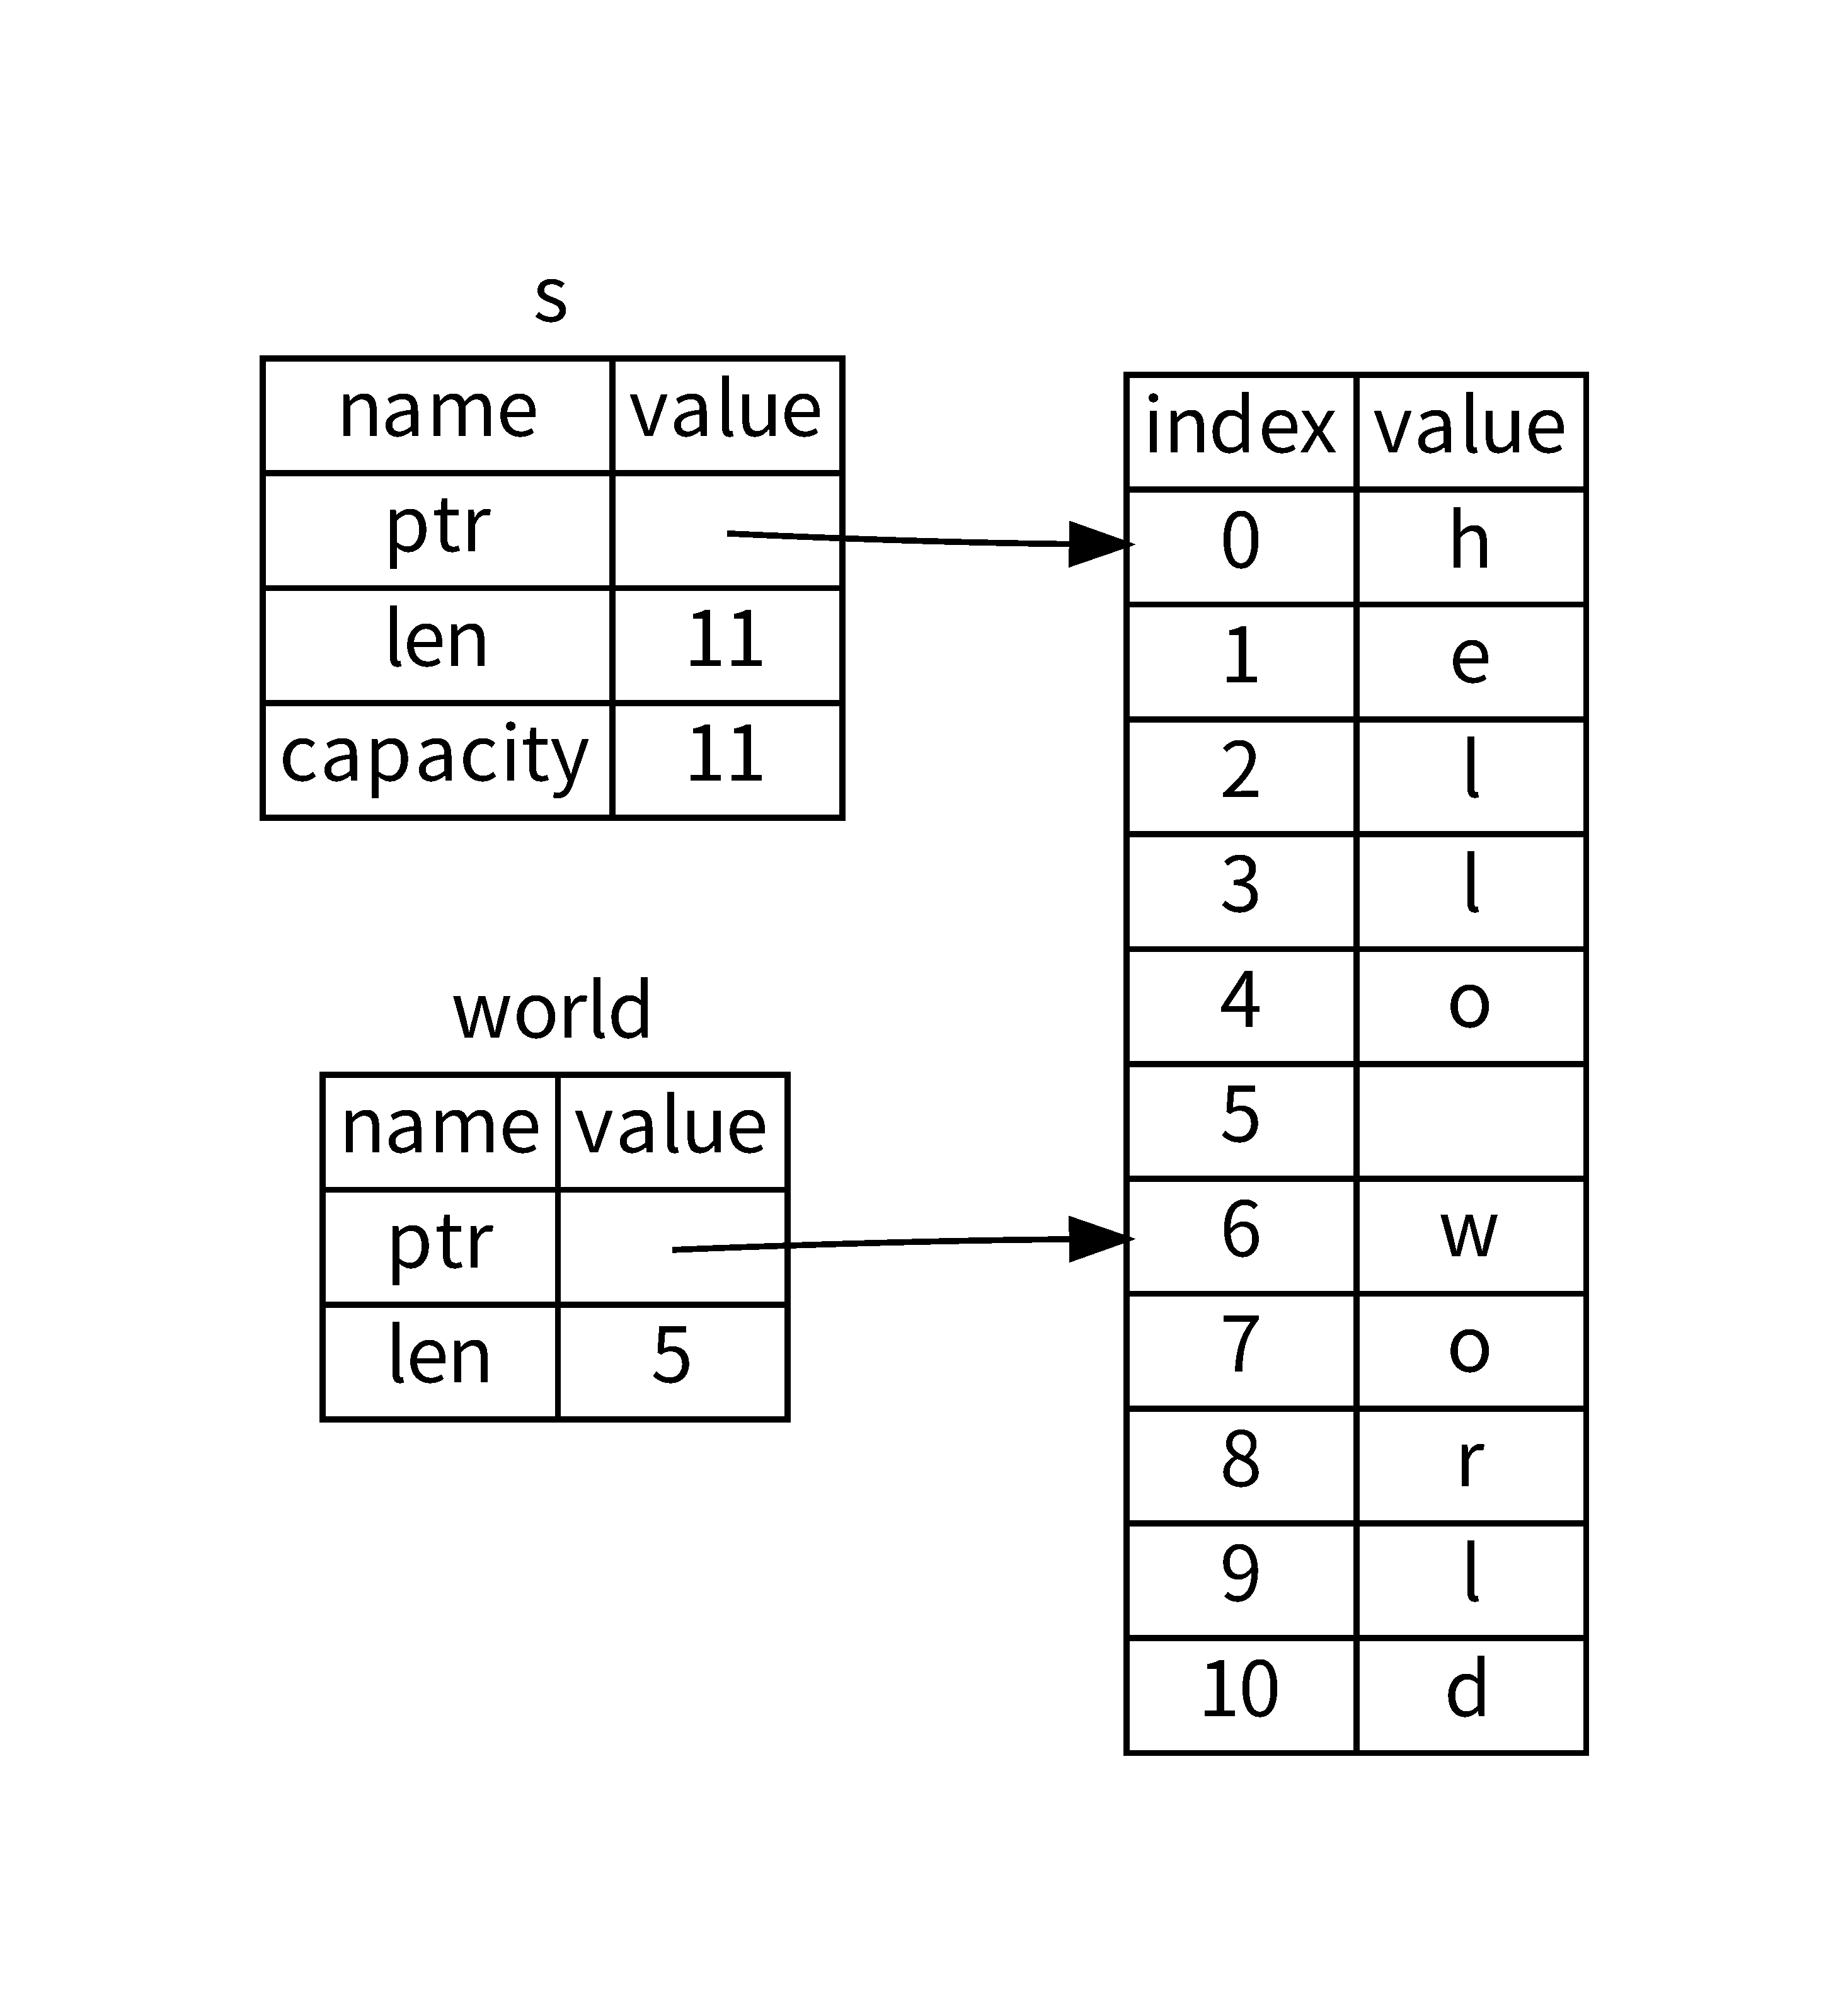
\includegraphics[width=0.5\textwidth,height=\textheight]{img/trpl04-06.pdf}

{Figure 4-6: String slice referring to part of a
\mintinline[]{text}{String}}

With Rust's \mintinline[]{text}{..} range syntax, if you want to start
at the first index (zero), you can drop the value before the two
periods. In other words, these are equal:

\begin{minted}[]{rust}
let s = String::from("hello");

let slice = &s[0..2];
let slice = &s[..2];
\end{minted}

By the same token, if your slice includes the last byte of the
\mintinline[]{text}{String}, you can drop the trailing number. That
means these are equal:

\begin{minted}[]{rust}
let s = String::from("hello");

let len = s.len();

let slice = &s[3..len];
let slice = &s[3..];
\end{minted}

You can also drop both values to take a slice of the entire string. So
these are equal:

\begin{minted}[]{rust}
let s = String::from("hello");

let len = s.len();

let slice = &s[0..len];
let slice = &s[..];
\end{minted}

\begin{quote}
Note: String slice range indices must occur at valid UTF-8 character
boundaries. If you attempt to create a string slice in the middle of a
multibyte character, your program will exit with an error. For the
purposes of introducing string slices, we are assuming ASCII only in
this section; a more thorough discussion of UTF-8 handling is in the
\href{ch08-02-strings.html\#storing-utf-8-encoded-text-with-strings}{``Storing
UTF-8 Encoded Text with Strings''} section of Chapter 8.
\end{quote}

With all this information in mind, let's rewrite
\mintinline[]{text}{first_word} to return a slice. The type that
signifies ``string slice'' is written as \mintinline[]{text}{&str}:

{Filename: src/main.rs}

\begin{minted}[]{rust}
fn first_word(s: &String) -> &str {
    let bytes = s.as_bytes();

    for (i, &item) in bytes.iter().enumerate() {
        if item == b' ' {
            return &s[0..i];
        }
    }

    &s[..]
}
\end{minted}

We get the index for the end of the word in the same way as we did in
Listing 4-7, by looking for the first occurrence of a space. When we
find a space, we return a string slice using the start of the string and
the index of the space as the starting and ending indices.

Now when we call \mintinline[]{text}{first_word}, we get back a single
value that is tied to the underlying data. The value is made up of a
reference to the starting point of the slice and the number of elements
in the slice.

Returning a slice would also work for a \mintinline[]{text}{second_word}
function:

\begin{minted}[]{rust}
fn second_word(s: &String) -> &str {
\end{minted}

We now have a straightforward API that's much harder to mess up, because
the compiler will ensure the references into the
\mintinline[]{text}{String} remain valid. Remember the bug in the
program in Listing 4-8, when we got the index to the end of the first
word but then cleared the string so our index was invalid? That code was
logically incorrect but didn't show any immediate errors. The problems
would show up later if we kept trying to use the first word index with
an emptied string. Slices make this bug impossible and let us know we
have a problem with our code much sooner. Using the slice version of
\mintinline[]{text}{first_word} will throw a compile-time error:

{Filename: src/main.rs}

\begin{minted}[]{rust}
fn main() {
    let mut s = String::from("hello world");

    let word = first_word(&s);

    s.clear(); // error!

    println!("the first word is: {}", word);
}
\end{minted}

Here's the compiler error:

\begin{minted}[]{text}
error[E0502]: cannot borrow `s` as mutable because it is also borrowed as immutable
  --> src/main.rs:18:5
   |
16 |     let word = first_word(&s);
   |                           -- immutable borrow occurs here
17 |
18 |     s.clear(); // error!
   |     ^^^^^^^^^ mutable borrow occurs here
19 |
20 |     println!("the first word is: {}", word);
   |                                       ---- immutable borrow later used here
\end{minted}

Recall from the borrowing rules that if we have an immutable reference
to something, we cannot also take a mutable reference. Because
\mintinline[]{text}{clear} needs to truncate the
\mintinline[]{text}{String}, it needs to get a mutable reference. Rust
disallows this, and compilation fails. Not only has Rust made our API
easier to use, but it has also eliminated an entire class of errors at
compile time!

\hypertarget{string-literals-are-slices}{%
\paragraph{String Literals Are
Slices}\label{string-literals-are-slices}}

Recall that we talked about string literals being stored inside the
binary. Now that we know about slices, we can properly understand string
literals:

\begin{minted}[]{rust}
let s = "Hello, world!";
\end{minted}

The type of \mintinline[]{text}{s} here is \mintinline[]{text}{&str}:
it's a slice pointing to that specific point of the binary. This is also
why string literals are immutable; \mintinline[]{text}{&str} is an
immutable reference.

\hypertarget{string-slices-as-parameters}{%
\paragraph{String Slices as
Parameters}\label{string-slices-as-parameters}}

Knowing that you can take slices of literals and
\mintinline[]{text}{String} values leads us to one more improvement on
\mintinline[]{text}{first_word}, and that's its signature:

\begin{minted}[]{rust}
fn first_word(s: &String) -> &str {
\end{minted}

A more experienced Rustacean would write the signature shown in Listing
4-9 instead because it allows us to use the same function on both
\mintinline[]{text}{&String} values and \mintinline[]{text}{&str}
values.

\begin{minted}[]{rust}
fn first_word(s: &str) -> &str {
\end{minted}

{Listing 4-9: Improving the \mintinline[]{text}{first_word} function by
using a string slice for the type of the \mintinline[]{text}{s}
parameter}

If we have a string slice, we can pass that directly. If we have a
\mintinline[]{text}{String}, we can pass a slice of the entire
\mintinline[]{text}{String}. Defining a function to take a string slice
instead of a reference to a \mintinline[]{text}{String} makes our API
more general and useful without losing any functionality:

{Filename: src/main.rs}

\begin{minted}[]{rust}
# fn first_word(s: &str) -> &str {
#     let bytes = s.as_bytes();
#
#     for (i, &item) in bytes.iter().enumerate() {
#         if item == b' ' {
#             return &s[0..i];
#         }
#     }
#
#     &s[..]
# }
fn main() {
    let my_string = String::from("hello world");

    // first_word works on slices of `String`s
    let word = first_word(&my_string[..]);

    let my_string_literal = "hello world";

    // first_word works on slices of string literals
    let word = first_word(&my_string_literal[..]);

    // Because string literals *are* string slices already,
    // this works too, without the slice syntax!
    let word = first_word(my_string_literal);
}
\end{minted}

\hypertarget{other-slices}{%
\subsubsection{Other Slices}\label{other-slices}}

String slices, as you might imagine, are specific to strings. But
there's a more general slice type, too. Consider this array:

\begin{minted}[]{rust}
let a = [1, 2, 3, 4, 5];
\end{minted}

Just as we might want to refer to a part of a string, we might want to
refer to part of an array. We'd do so like this:

\begin{minted}[]{rust}
let a = [1, 2, 3, 4, 5];

let slice = &a[1..3];
\end{minted}

This slice has the type \mintinline[]{text}{&[i32]}. It works the same
way as string slices do, by storing a reference to the first element and
a length. You'll use this kind of slice for all sorts of other
collections. We'll discuss these collections in detail when we talk
about vectors in Chapter 8.

\hypertarget{summary-3}{%
\subsection{Summary}\label{summary-3}}

The concepts of ownership, borrowing, and slices ensure memory safety in
Rust programs at compile time. The Rust language gives you control over
your memory usage in the same way as other systems programming
languages, but having the owner of data automatically clean up that data
when the owner goes out of scope means you don't have to write and debug
extra code to get this control.

Ownership affects how lots of other parts of Rust work, so we'll talk
about these concepts further throughout the rest of the book. Let's move
on to Chapter 5 and look at grouping pieces of data together in a
\mintinline[]{text}{struct}.

\hypertarget{using-structs-to-structure-related-data}{%
\section{Using Structs to Structure Related
Data}\label{using-structs-to-structure-related-data}}

A \emph{struct}, or \emph{structure}, is a custom data type that lets
you name and package together multiple related values that make up a
meaningful group. If you're familiar with an object-oriented language, a
\emph{struct} is like an object's data attributes. In this chapter,
we'll compare and contrast tuples with structs, demonstrate how to use
structs, and discuss how to define methods and associated functions to
specify behavior associated with a struct's data. Structs and enums
(discussed in Chapter 6) are the building blocks for creating new types
in your program's domain to take full advantage of Rust's compile time
type checking.

\hypertarget{defining-and-instantiating-structs}{%
\subsection{Defining and Instantiating
Structs}\label{defining-and-instantiating-structs}}

Structs are similar to tuples, which were discussed in Chapter 3. Like
tuples, the pieces of a struct can be different types. Unlike with
tuples, you'll name each piece of data so it's clear what the values
mean. As a result of these names, structs are more flexible than tuples:
you don't have to rely on the order of the data to specify or access the
values of an instance.

To define a struct, we enter the keyword \mintinline[]{text}{struct} and
name the entire struct. A struct's name should describe the significance
of the pieces of data being grouped together. Then, inside curly
brackets, we define the names and types of the pieces of data, which we
call \emph{fields}. For example, Listing 5-1 shows a struct that stores
information about a user account.

\begin{minted}[]{rust}
struct User {
    username: String,
    email: String,
    sign_in_count: u64,
    active: bool,
}
\end{minted}

{Listing 5-1: A \mintinline[]{text}{User} struct definition}

To use a struct after we've defined it, we create an \emph{instance} of
that struct by specifying concrete values for each of the fields. We
create an instance by stating the name of the struct and then add curly
brackets containing \mintinline[]{text}{key: value} pairs, where the
keys are the names of the fields and the values are the data we want to
store in those fields. We don't have to specify the fields in the same
order in which we declared them in the struct. In other words, the
struct definition is like a general template for the type, and instances
fill in that template with particular data to create values of the type.
For example, we can declare a particular user as shown in Listing 5-2.

\begin{minted}[]{rust}
# struct User {
#     username: String,
#     email: String,
#     sign_in_count: u64,
#     active: bool,
# }
#
let user1 = User {
    email: String::from("someone@example.com"),
    username: String::from("someusername123"),
    active: true,
    sign_in_count: 1,
};
\end{minted}

{Listing 5-2: Creating an instance of the \mintinline[]{text}{User}
struct}

To get a specific value from a struct, we can use dot notation. If we
wanted just this user's email address, we could use
\mintinline[]{text}{user1.email} wherever we wanted to use this value.
If the instance is mutable, we can change a value by using the dot
notation and assigning into a particular field. Listing 5-3 shows how to
change the value in the \mintinline[]{text}{email} field of a mutable
\mintinline[]{text}{User} instance.

\begin{minted}[]{rust}
# struct User {
#     username: String,
#     email: String,
#     sign_in_count: u64,
#     active: bool,
# }
#
let mut user1 = User {
    email: String::from("someone@example.com"),
    username: String::from("someusername123"),
    active: true,
    sign_in_count: 1,
};

user1.email = String::from("anotheremail@example.com");
\end{minted}

{Listing 5-3: Changing the value in the \mintinline[]{text}{email} field
of a \mintinline[]{text}{User} instance}

Note that the entire instance must be mutable; Rust doesn't allow us to
mark only certain fields as mutable. As with any expression, we can
construct a new instance of the struct as the last expression in the
function body to implicitly return that new instance.

Listing 5-4 shows a \mintinline[]{text}{build_user} function that
returns a \mintinline[]{text}{User} instance with the given email and
username. The \mintinline[]{text}{active} field gets the value of
\mintinline[]{text}{true}, and the \mintinline[]{text}{sign_in_count}
gets a value of \mintinline[]{text}{1}.

\begin{minted}[]{rust}
# struct User {
#     username: String,
#     email: String,
#     sign_in_count: u64,
#     active: bool,
# }
#
fn build_user(email: String, username: String) -> User {
    User {
        email: email,
        username: username,
        active: true,
        sign_in_count: 1,
    }
}
\end{minted}

{Listing 5-4: A \mintinline[]{text}{build_user} function that takes an
email and username and returns a \mintinline[]{text}{User} instance}

It makes sense to name the function parameters with the same name as the
struct fields, but having to repeat the \mintinline[]{text}{email} and
\mintinline[]{text}{username} field names and variables is a bit
tedious. If the struct had more fields, repeating each name would get
even more annoying. Luckily, there's a convenient shorthand!

\hypertarget{using-the-field-init-shorthand-when-variables-and-fields-have-the-same-name}{%
\subsubsection{Using the Field Init Shorthand when Variables and Fields
Have the Same
Name}\label{using-the-field-init-shorthand-when-variables-and-fields-have-the-same-name}}

Because the parameter names and the struct field names are exactly the
same in Listing 5-4, we can use the \emph{field init shorthand} syntax
to rewrite \mintinline[]{text}{build_user} so that it behaves exactly
the same but doesn't have the repetition of \mintinline[]{text}{email}
and \mintinline[]{text}{username}, as shown in Listing 5-5.

\begin{minted}[]{rust}
# struct User {
#     username: String,
#     email: String,
#     sign_in_count: u64,
#     active: bool,
# }
#
fn build_user(email: String, username: String) -> User {
    User {
        email,
        username,
        active: true,
        sign_in_count: 1,
    }
}
\end{minted}

{Listing 5-5: A \mintinline[]{text}{build_user} function that uses field
init shorthand because the \mintinline[]{text}{email} and
\mintinline[]{text}{username} parameters have the same name as struct
fields}

Here, we're creating a new instance of the \mintinline[]{text}{User}
struct, which has a field named \mintinline[]{text}{email}. We want to
set the \mintinline[]{text}{email} field's value to the value in the
\mintinline[]{text}{email} parameter of the
\mintinline[]{text}{build_user} function. Because the
\mintinline[]{text}{email} field and the \mintinline[]{text}{email}
parameter have the same name, we only need to write
\mintinline[]{text}{email} rather than
\mintinline[]{text}{email: email}.

\hypertarget{creating-instances-from-other-instances-with-struct-update-syntax}{%
\subsubsection{Creating Instances From Other Instances With Struct
Update
Syntax}\label{creating-instances-from-other-instances-with-struct-update-syntax}}

It's often useful to create a new instance of a struct that uses most of
an old instance's values but changes some. You'll do this using
\emph{struct update syntax}.

First, Listing 5-6 shows how we create a new \mintinline[]{text}{User}
instance in \mintinline[]{text}{user2} without the update syntax. We set
new values for \mintinline[]{text}{email} and
\mintinline[]{text}{username} but otherwise use the same values from
\mintinline[]{text}{user1} that we created in Listing 5-2.

\begin{minted}[]{rust}
# struct User {
#     username: String,
#     email: String,
#     sign_in_count: u64,
#     active: bool,
# }
#
# let user1 = User {
#     email: String::from("someone@example.com"),
#     username: String::from("someusername123"),
#     active: true,
#     sign_in_count: 1,
# };
#
let user2 = User {
    email: String::from("another@example.com"),
    username: String::from("anotherusername567"),
    active: user1.active,
    sign_in_count: user1.sign_in_count,
};
\end{minted}

{Listing 5-6: Creating a new \mintinline[]{text}{User} instance using
some of the values from \mintinline[]{text}{user1}}

Using struct update syntax, we can achieve the same effect with less
code, as shown in Listing 5-7. The syntax \mintinline[]{text}{..}
specifies that the remaining fields not explicitly set should have the
same value as the fields in the given instance.

\begin{minted}[]{rust}
# struct User {
#     username: String,
#     email: String,
#     sign_in_count: u64,
#     active: bool,
# }
#
# let user1 = User {
#     email: String::from("someone@example.com"),
#     username: String::from("someusername123"),
#     active: true,
#     sign_in_count: 1,
# };
#
let user2 = User {
    email: String::from("another@example.com"),
    username: String::from("anotherusername567"),
    ..user1
};
\end{minted}

{Listing 5-7: Using struct update syntax to set new
\mintinline[]{text}{email} and \mintinline[]{text}{username} values for
a \mintinline[]{text}{User} instance but use the rest of the values from
the fields of the instance in the \mintinline[]{text}{user1} variable}

The code in Listing 5-7 also creates an instance in
\mintinline[]{text}{user2} that has a different value for
\mintinline[]{text}{email} and \mintinline[]{text}{username} but has the
same values for the \mintinline[]{text}{active} and
\mintinline[]{text}{sign_in_count} fields from
\mintinline[]{text}{user1}.

\hypertarget{using-tuple-structs-without-named-fields-to-create-different-types}{%
\subsubsection{Using Tuple Structs without Named Fields to Create
Different
Types}\label{using-tuple-structs-without-named-fields-to-create-different-types}}

You can also define structs that look similar to tuples, called
\emph{tuple structs}. Tuple structs have the added meaning the struct
name provides but don't have names associated with their fields; rather,
they just have the types of the fields. Tuple structs are useful when
you want to give the whole tuple a name and make the tuple be a
different type from other tuples, and naming each field as in a regular
struct would be verbose or redundant.

To define a tuple struct, start with the \mintinline[]{text}{struct}
keyword and the struct name followed by the types in the tuple. For
example, here are definitions and usages of two tuple structs named
\mintinline[]{text}{Color} and \mintinline[]{text}{Point}:

\begin{minted}[]{rust}
struct Color(i32, i32, i32);
struct Point(i32, i32, i32);

let black = Color(0, 0, 0);
let origin = Point(0, 0, 0);
\end{minted}

Note that the \mintinline[]{text}{black} and \mintinline[]{text}{origin}
values are different types, because they're instances of different tuple
structs. Each struct you define is its own type, even though the fields
within the struct have the same types. For example, a function that
takes a parameter of type \mintinline[]{text}{Color} cannot take a
\mintinline[]{text}{Point} as an argument, even though both types are
made up of three \mintinline[]{text}{i32} values. Otherwise, tuple
struct instances behave like tuples: you can destructure them into their
individual pieces, you can use a \mintinline[]{text}{.} followed by the
index to access an individual value, and so on.

\hypertarget{unit-like-structs-without-any-fields}{%
\subsubsection{Unit-Like Structs Without Any
Fields}\label{unit-like-structs-without-any-fields}}

You can also define structs that don't have any fields! These are called
\emph{unit-like structs} because they behave similarly to
\mintinline[]{text}{()}, the unit type. Unit-like structs can be useful
in situations in which you need to implement a trait on some type but
don't have any data that you want to store in the type itself. We'll
discuss traits in Chapter 10.

\begin{quote}
\hypertarget{ownership-of-struct-data}{%
\subsubsection{Ownership of Struct
Data}\label{ownership-of-struct-data}}

In the \mintinline[]{text}{User} struct definition in Listing 5-1, we
used the owned \mintinline[]{text}{String} type rather than the
\mintinline[]{text}{&str} string slice type. This is a deliberate choice
because we want instances of this struct to own all of its data and for
that data to be valid for as long as the entire struct is valid.

It's possible for structs to store references to data owned by something
else, but to do so requires the use of \emph{lifetimes}, a Rust feature
that we'll discuss in Chapter 10. Lifetimes ensure that the data
referenced by a struct is valid for as long as the struct is. Let's say
you try to store a reference in a struct without specifying lifetimes,
like this, which won't work:

{Filename: src/main.rs}

\begin{minted}[]{rust}
struct User {
    username: &str,
    email: &str,
    sign_in_count: u64,
    active: bool,
}

fn main() {
    let user1 = User {
        email: "someone@example.com",
        username: "someusername123",
        active: true,
        sign_in_count: 1,
    };
}
\end{minted}

The compiler will complain that it needs lifetime specifiers:

\begin{minted}[]{text}
error[E0106]: missing lifetime specifier
 -->
  |
2 |     username: &str,
  |               ^ expected lifetime parameter

error[E0106]: missing lifetime specifier
 -->
  |
3 |     email: &str,
  |            ^ expected lifetime parameter
\end{minted}

In Chapter 10, we'll discuss how to fix these errors so you can store
references in structs, but for now, we'll fix errors like these using
owned types like \mintinline[]{text}{String} instead of references like
\mintinline[]{text}{&str}.
\end{quote}

\hypertarget{an-example-program-using-structs}{%
\subsection{An Example Program Using
Structs}\label{an-example-program-using-structs}}

To understand when we might want to use structs, let's write a program
that calculates the area of a rectangle. We'll start with single
variables, and then refactor the program until we're using structs
instead.

Let's make a new binary project with Cargo called \emph{rectangles} that
will take the width and height of a rectangle specified in pixels and
calculate the area of the rectangle. Listing 5-8 shows a short program
with one way of doing exactly that in our project's \emph{src/main.rs}.

{Filename: src/main.rs}

\begin{minted}[]{rust}
fn main() {
    let width1 = 30;
    let height1 = 50;

    println!(
        "The area of the rectangle is {} square pixels.",
        area(width1, height1)
    );
}

fn area(width: u32, height: u32) -> u32 {
    width * height
}
\end{minted}

{Listing 5-8: Calculating the area of a rectangle specified by separate
width and height variables}

Now, run this program using \mintinline[]{text}{cargo run}:

\begin{minted}[]{text}
The area of the rectangle is 1500 square pixels.
\end{minted}

Even though Listing 5-8 works and figures out the area of the rectangle
by calling the \mintinline[]{text}{area} function with each dimension,
we can do better. The width and the height are related to each other
because together they describe one rectangle.

The issue with this code is evident in the signature of
\mintinline[]{text}{area}:

\begin{minted}[]{rust}
fn area(width: u32, height: u32) -> u32 {
\end{minted}

The \mintinline[]{text}{area} function is supposed to calculate the area
of one rectangle, but the function we wrote has two parameters. The
parameters are related, but that's not expressed anywhere in our
program. It would be more readable and more manageable to group width
and height together. We've already discussed one way we might do that in
\href{ch03-02-data-types.html\#the-tuple-type}{``The Tuple Type''}
section of Chapter 3: by using tuples.

\hypertarget{refactoring-with-tuples}{%
\subsubsection{Refactoring with Tuples}\label{refactoring-with-tuples}}

Listing 5-9 shows another version of our program that uses tuples.

{Filename: src/main.rs}

\begin{minted}[]{rust}
fn main() {
    let rect1 = (30, 50);

    println!(
        "The area of the rectangle is {} square pixels.",
        area(rect1)
    );
}

fn area(dimensions: (u32, u32)) -> u32 {
    dimensions.0 * dimensions.1
}
\end{minted}

{Listing 5-9: Specifying the width and height of the rectangle with a
tuple}

In one way, this program is better. Tuples let us add a bit of
structure, and we're now passing just one argument. But in another way,
this version is less clear: tuples don't name their elements, so our
calculation has become more confusing because we have to index into the
parts of the tuple.

It doesn't matter if we mix up width and height for the area
calculation, but if we want to draw the rectangle on the screen, it
would matter! We would have to keep in mind that
\mintinline[]{text}{width} is the tuple index \mintinline[]{text}{0} and
\mintinline[]{text}{height} is the tuple index \mintinline[]{text}{1}.
If someone else worked on this code, they would have to figure this out
and keep it in mind as well. It would be easy to forget or mix up these
values and cause errors, because we haven't conveyed the meaning of our
data in our code.

\hypertarget{refactoring-with-structs-adding-more-meaning}{%
\subsubsection{Refactoring with Structs: Adding More
Meaning}\label{refactoring-with-structs-adding-more-meaning}}

We use structs to add meaning by labeling the data. We can transform the
tuple we're using into a data type with a name for the whole as well as
names for the parts, as shown in Listing 5-10.

{Filename: src/main.rs}

\begin{minted}[]{rust}
struct Rectangle {
    width: u32,
    height: u32,
}

fn main() {
    let rect1 = Rectangle { width: 30, height: 50 };

    println!(
        "The area of the rectangle is {} square pixels.",
        area(&rect1)
    );
}

fn area(rectangle: &Rectangle) -> u32 {
    rectangle.width * rectangle.height
}
\end{minted}

{Listing 5-10: Defining a \mintinline[]{text}{Rectangle} struct}

Here we've defined a struct and named it \mintinline[]{text}{Rectangle}.
Inside the curly brackets, we defined the fields as
\mintinline[]{text}{width} and \mintinline[]{text}{height}, both of
which have type \mintinline[]{text}{u32}. Then in
\mintinline[]{text}{main}, we created a particular instance of
\mintinline[]{text}{Rectangle} that has a width of 30 and a height of
50.

Our \mintinline[]{text}{area} function is now defined with one
parameter, which we've named \mintinline[]{text}{rectangle}, whose type
is an immutable borrow of a struct \mintinline[]{text}{Rectangle}
instance. As mentioned in Chapter 4, we want to borrow the struct rather
than take ownership of it. This way, \mintinline[]{text}{main} retains
its ownership and can continue using \mintinline[]{text}{rect1}, which
is the reason we use the \mintinline[]{text}{&} in the function
signature and where we call the function.

The \mintinline[]{text}{area} function accesses the
\mintinline[]{text}{width} and \mintinline[]{text}{height} fields of the
\mintinline[]{text}{Rectangle} instance. Our function signature for
\mintinline[]{text}{area} now says exactly what we mean: calculate the
area of \mintinline[]{text}{Rectangle}, using its
\mintinline[]{text}{width} and \mintinline[]{text}{height} fields. This
conveys that the width and height are related to each other, and it
gives descriptive names to the values rather than using the tuple index
values of \mintinline[]{text}{0} and \mintinline[]{text}{1}. This is a
win for clarity.

\hypertarget{adding-useful-functionality-with-derived-traits}{%
\subsubsection{Adding Useful Functionality with Derived
Traits}\label{adding-useful-functionality-with-derived-traits}}

It'd be nice to be able to print an instance of
\mintinline[]{text}{Rectangle} while we're debugging our program and see
the values for all its fields. Listing 5-11 tries using the
\mintinline[]{text}{println!} macro as we have used in previous
chapters. This won't work, however.

{Filename: src/main.rs}

\begin{minted}[]{rust}
struct Rectangle {
    width: u32,
    height: u32,
}

fn main() {
    let rect1 = Rectangle { width: 30, height: 50 };

    println!("rect1 is {}", rect1);
}
\end{minted}

{Listing 5-11: Attempting to print a \mintinline[]{text}{Rectangle}
instance}

When we compile this code, we get an error with this core message:

\begin{minted}[]{text}
error[E0277]: `Rectangle` doesn't implement `std::fmt::Display`
\end{minted}

The \mintinline[]{text}{println!} macro can do many kinds of formatting,
and by default, the curly brackets tell \mintinline[]{text}{println!} to
use formatting known as \mintinline[]{text}{Display}: output intended
for direct end user consumption. The primitive types we've seen so far
implement \mintinline[]{text}{Display} by default, because there's only
one way you'd want to show a \mintinline[]{text}{1} or any other
primitive type to a user. But with structs, the way
\mintinline[]{text}{println!} should format the output is less clear
because there are more display possibilities: Do you want commas or not?
Do you want to print the curly brackets? Should all the fields be shown?
Due to this ambiguity, Rust doesn't try to guess what we want, and
structs don't have a provided implementation of
\mintinline[]{text}{Display}.

If we continue reading the errors, we'll find this helpful note:

\begin{minted}[]{text}
= help: the trait `std::fmt::Display` is not implemented for `Rectangle`
= note: in format strings you may be able to use `{:?}` (or {:#?} for pretty-print) instead
\end{minted}

Let's try it! The \mintinline[]{text}{println!} macro call will now look
like \mintinline[]{text}{println!("rect1 is {:?}", rect1);}. Putting the
specifier \mintinline[]{text}{:?} inside the curly brackets tells
\mintinline[]{text}{println!} we want to use an output format called
\mintinline[]{text}{Debug}. The \mintinline[]{text}{Debug} trait enables
us to print our struct in a way that is useful for developers so we can
see its value while we're debugging our code.

Compile the code with this change. Drat! We still get an error:

\begin{minted}[]{text}
error[E0277]: `Rectangle` doesn't implement `std::fmt::Debug`
\end{minted}

But again, the compiler gives us a helpful note:

\begin{minted}[]{text}
= help: the trait `std::fmt::Debug` is not implemented for `Rectangle`
= note: add `#[derive(Debug)]` or manually implement `std::fmt::Debug`
\end{minted}

Rust \emph{does} include functionality to print out debugging
information, but we have to explicitly opt in to make that functionality
available for our struct. To do that, we add the annotation
\mintinline[]{text}{#[derive(Debug)]} just before the struct definition,
as shown in Listing 5-12.

{Filename: src/main.rs}

\begin{minted}[]{rust}
#[derive(Debug)]
struct Rectangle {
    width: u32,
    height: u32,
}

fn main() {
    let rect1 = Rectangle { width: 30, height: 50 };

    println!("rect1 is {:?}", rect1);
}
\end{minted}

{Listing 5-12: Adding the annotation to derive the
\mintinline[]{text}{Debug} trait and printing the
\mintinline[]{text}{Rectangle} instance using debug formatting}

Now when we run the program, we won't get any errors, and we'll see the
following output:

\begin{minted}[]{text}
rect1 is Rectangle { width: 30, height: 50 }
\end{minted}

Nice! It's not the prettiest output, but it shows the values of all the
fields for this instance, which would definitely help during debugging.
When we have larger structs, it's useful to have output that's a bit
easier to read; in those cases, we can use \mintinline[]{text}{{:#?}}
instead of \mintinline[]{text}{{:?}} in the
\mintinline[]{text}{println!} string. When we use the
\mintinline[]{text}{{:#?}} style in the example, the output will look
like this:

\begin{minted}[]{text}
rect1 is Rectangle {
    width: 30,
    height: 50
}
\end{minted}

Rust has provided a number of traits for us to use with the
\mintinline[]{text}{derive} annotation that can add useful behavior to
our custom types. Those traits and their behaviors are listed in
Appendix C. We'll cover how to implement these traits with custom
behavior as well as how to create your own traits in Chapter 10.

Our \mintinline[]{text}{area} function is very specific: it only
computes the area of rectangles. It would be helpful to tie this
behavior more closely to our \mintinline[]{text}{Rectangle} struct,
because it won't work with any other type. Let's look at how we can
continue to refactor this code by turning the \mintinline[]{text}{area}
function into an \mintinline[]{text}{area} \emph{method} defined on our
\mintinline[]{text}{Rectangle} type.

\hypertarget{method-syntax}{%
\subsection{Method Syntax}\label{method-syntax}}

\emph{Methods} are similar to functions: they're declared with the
\mintinline[]{text}{fn} keyword and their name, they can have parameters
and a return value, and they contain some code that is run when they're
called from somewhere else. However, methods are different from
functions in that they're defined within the context of a struct (or an
enum or a trait object, which we cover in Chapters 6 and 17,
respectively), and their first parameter is always
\mintinline[]{text}{self}, which represents the instance of the struct
the method is being called on.

\hypertarget{defining-methods}{%
\subsubsection{Defining Methods}\label{defining-methods}}

Let's change the \mintinline[]{text}{area} function that has a
\mintinline[]{text}{Rectangle} instance as a parameter and instead make
an \mintinline[]{text}{area} method defined on the
\mintinline[]{text}{Rectangle} struct, as shown in Listing 5-13.

{Filename: src/main.rs}

\begin{minted}[]{rust}
#[derive(Debug)]
struct Rectangle {
    width: u32,
    height: u32,
}

impl Rectangle {
    fn area(&self) -> u32 {
        self.width * self.height
    }
}

fn main() {
    let rect1 = Rectangle { width: 30, height: 50 };

    println!(
        "The area of the rectangle is {} square pixels.",
        rect1.area()
    );
}
\end{minted}

{Listing 5-13: Defining an \mintinline[]{text}{area} method on the
\mintinline[]{text}{Rectangle} struct}

To define the function within the context of
\mintinline[]{text}{Rectangle}, we start an \mintinline[]{text}{impl}
(implementation) block. Then we move the \mintinline[]{text}{area}
function within the \mintinline[]{text}{impl} curly brackets and change
the first (and in this case, only) parameter to be
\mintinline[]{text}{self} in the signature and everywhere within the
body. In \mintinline[]{text}{main}, where we called the
\mintinline[]{text}{area} function and passed \mintinline[]{text}{rect1}
as an argument, we can instead use \emph{method syntax} to call the
\mintinline[]{text}{area} method on our \mintinline[]{text}{Rectangle}
instance. The method syntax goes after an instance: we add a dot
followed by the method name, parentheses, and any arguments.

In the signature for \mintinline[]{text}{area}, we use
\mintinline[]{text}{&self} instead of
\mintinline[]{text}{rectangle: &Rectangle} because Rust knows the type
of \mintinline[]{text}{self} is \mintinline[]{text}{Rectangle} due to
this method's being inside the \mintinline[]{text}{impl Rectangle}
context. Note that we still need to use the \mintinline[]{text}{&}
before \mintinline[]{text}{self}, just as we did in
\mintinline[]{text}{&Rectangle}. Methods can take ownership of
\mintinline[]{text}{self}, borrow \mintinline[]{text}{self} immutably as
we've done here, or borrow \mintinline[]{text}{self} mutably, just as
they can any other parameter.

We've chosen \mintinline[]{text}{&self} here for the same reason we used
\mintinline[]{text}{&Rectangle} in the function version: we don't want
to take ownership, and we just want to read the data in the struct, not
write to it. If we wanted to change the instance that we've called the
method on as part of what the method does, we'd use
\mintinline[]{text}{&mut self} as the first parameter. Having a method
that takes ownership of the instance by using just
\mintinline[]{text}{self} as the first parameter is rare; this technique
is usually used when the method transforms \mintinline[]{text}{self}
into something else and you want to prevent the caller from using the
original instance after the transformation.

The main benefit of using methods instead of functions, in addition to
using method syntax and not having to repeat the type of
\mintinline[]{text}{self} in every method's signature, is for
organization. We've put all the things we can do with an instance of a
type in one \mintinline[]{text}{impl} block rather than making future
users of our code search for capabilities of
\mintinline[]{text}{Rectangle} in various places in the library we
provide.

\begin{quote}
\hypertarget{wheres-the---operator}{%
\subsubsection{\texorpdfstring{Where's the \mintinline[]{text}{->}
Operator?}{Where's the  Operator?}}\label{wheres-the---operator}}

In C and C++, two different operators are used for calling methods: you
use \mintinline[]{text}{.} if you're calling a method on the object
directly and \mintinline[]{text}{->} if you're calling the method on a
pointer to the object and need to dereference the pointer first. In
other words, if \mintinline[]{text}{object} is a pointer,
\mintinline[]{text}{object->something()} is similar to
\mintinline[]{text}{(*object).something()}.

Rust doesn't have an equivalent to the \mintinline[]{text}{->} operator;
instead, Rust has a feature called \emph{automatic referencing and
dereferencing}. Calling methods is one of the few places in Rust that
has this behavior.

Here's how it works: when you call a method with
\mintinline[]{text}{object.something()}, Rust automatically adds in
\mintinline[]{text}{&}, \mintinline[]{text}{&mut}, or
\mintinline[]{text}{*} so \mintinline[]{text}{object} matches the
signature of the method. In other words, the following are the same:

\begin{minted}[]{rust}
# #[derive(Debug,Copy,Clone)]
# struct Point {
#     x: f64,
#     y: f64,
# }
#
# impl Point {
#    fn distance(&self, other: &Point) -> f64 {
#        let x_squared = f64::powi(other.x - self.x, 2);
#        let y_squared = f64::powi(other.y - self.y, 2);
#
#        f64::sqrt(x_squared + y_squared)
#    }
# }
# let p1 = Point { x: 0.0, y: 0.0 };
# let p2 = Point { x: 5.0, y: 6.5 };
p1.distance(&p2);
(&p1).distance(&p2);
\end{minted}

The first one looks much cleaner. This automatic referencing behavior
works because methods have a clear receiver---the type of
\mintinline[]{text}{self}. Given the receiver and name of a method, Rust
can figure out definitively whether the method is reading
(\mintinline[]{text}{&self}), mutating (\mintinline[]{text}{&mut self}),
or consuming (\mintinline[]{text}{self}). The fact that Rust makes
borrowing implicit for method receivers is a big part of making
ownership ergonomic in practice.
\end{quote}

\hypertarget{methods-with-more-parameters}{%
\subsubsection{Methods with More
Parameters}\label{methods-with-more-parameters}}

Let's practice using methods by implementing a second method on the
\mintinline[]{text}{Rectangle} struct. This time, we want an instance of
\mintinline[]{text}{Rectangle} to take another instance of
\mintinline[]{text}{Rectangle} and return \mintinline[]{text}{true} if
the second \mintinline[]{text}{Rectangle} can fit completely within
\mintinline[]{text}{self}; otherwise it should return
\mintinline[]{text}{false}. That is, we want to be able to write the
program shown in Listing 5-14, once we've defined the
\mintinline[]{text}{can_hold} method.

{Filename: src/main.rs}

\begin{minted}[]{rust}
fn main() {
    let rect1 = Rectangle { width: 30, height: 50 };
    let rect2 = Rectangle { width: 10, height: 40 };
    let rect3 = Rectangle { width: 60, height: 45 };

    println!("Can rect1 hold rect2? {}", rect1.can_hold(&rect2));
    println!("Can rect1 hold rect3? {}", rect1.can_hold(&rect3));
}
\end{minted}

{Listing 5-14: Using the as-yet-unwritten \mintinline[]{text}{can_hold}
method}

And the expected output would look like the following, because both
dimensions of \mintinline[]{text}{rect2} are smaller than the dimensions
of \mintinline[]{text}{rect1} but \mintinline[]{text}{rect3} is wider
than \mintinline[]{text}{rect1}:

\begin{minted}[]{text}
Can rect1 hold rect2? true
Can rect1 hold rect3? false
\end{minted}

We know we want to define a method, so it will be within the
\mintinline[]{text}{impl Rectangle} block. The method name will be
\mintinline[]{text}{can_hold}, and it will take an immutable borrow of
another \mintinline[]{text}{Rectangle} as a parameter. We can tell what
the type of the parameter will be by looking at the code that calls the
method: \mintinline[]{text}{rect1.can_hold(&rect2)} passes in
\mintinline[]{text}{&rect2}, which is an immutable borrow to
\mintinline[]{text}{rect2}, an instance of
\mintinline[]{text}{Rectangle}. This makes sense because we only need to
read \mintinline[]{text}{rect2} (rather than write, which would mean
we'd need a mutable borrow), and we want \mintinline[]{text}{main} to
retain ownership of \mintinline[]{text}{rect2} so we can use it again
after calling the \mintinline[]{text}{can_hold} method. The return value
of \mintinline[]{text}{can_hold} will be a Boolean, and the
implementation will check whether the width and height of
\mintinline[]{text}{self} are both greater than the width and height of
the other \mintinline[]{text}{Rectangle}, respectively. Let's add the
new \mintinline[]{text}{can_hold} method to the
\mintinline[]{text}{impl} block from Listing 5-13, shown in Listing
5-15.

{Filename: src/main.rs}

\begin{minted}[]{rust}
# #[derive(Debug)]
# struct Rectangle {
#     width: u32,
#     height: u32,
# }
#
impl Rectangle {
    fn area(&self) -> u32 {
        self.width * self.height
    }

    fn can_hold(&self, other: &Rectangle) -> bool {
        self.width > other.width && self.height > other.height
    }
}
\end{minted}

{Listing 5-15: Implementing the \mintinline[]{text}{can_hold} method on
\mintinline[]{text}{Rectangle} that takes another
\mintinline[]{text}{Rectangle} instance as a parameter}

When we run this code with the \mintinline[]{text}{main} function in
Listing 5-14, we'll get our desired output. Methods can take multiple
parameters that we add to the signature after the
\mintinline[]{text}{self} parameter, and those parameters work just like
parameters in functions.

\hypertarget{associated-functions}{%
\subsubsection{Associated Functions}\label{associated-functions}}

Another useful feature of \mintinline[]{text}{impl} blocks is that we're
allowed to define functions within \mintinline[]{text}{impl} blocks that
\emph{don't} take \mintinline[]{text}{self} as a parameter. These are
called \emph{associated functions} because they're associated with the
struct. They're still functions, not methods, because they don't have an
instance of the struct to work with. You've already used the
\mintinline[]{text}{String::from} associated function.

Associated functions are often used for constructors that will return a
new instance of the struct. For example, we could provide an associated
function that would have one dimension parameter and use that as both
width and height, thus making it easier to create a square
\mintinline[]{text}{Rectangle} rather than having to specify the same
value twice:

{Filename: src/main.rs}

\begin{minted}[]{rust}
# #[derive(Debug)]
# struct Rectangle {
#     width: u32,
#     height: u32,
# }
#
impl Rectangle {
    fn square(size: u32) -> Rectangle {
        Rectangle { width: size, height: size }
    }
}
\end{minted}

To call this associated function, we use the \mintinline[]{text}{::}
syntax with the struct name;
\mintinline[]{text}{let sq = Rectangle::square(3);} is an example. This
function is namespaced by the struct: the \mintinline[]{text}{::} syntax
is used for both associated functions and namespaces created by modules.
We'll discuss modules in Chapter 7.

\hypertarget{multiple-impl-blocks}{%
\subsubsection{\texorpdfstring{Multiple \mintinline[]{text}{impl}
Blocks}{Multiple  Blocks}}\label{multiple-impl-blocks}}

Each struct is allowed to have multiple \mintinline[]{text}{impl}
blocks. For example, Listing 5-15 is equivalent to the code shown in
Listing 5-16, which has each method in its own \mintinline[]{text}{impl}
block.

\begin{minted}[]{rust}
# #[derive(Debug)]
# struct Rectangle {
#     width: u32,
#     height: u32,
# }
#
impl Rectangle {
    fn area(&self) -> u32 {
        self.width * self.height
    }
}

impl Rectangle {
    fn can_hold(&self, other: &Rectangle) -> bool {
        self.width > other.width && self.height > other.height
    }
}
\end{minted}

{Listing 5-16: Rewriting Listing 5-15 using multiple
\mintinline[]{text}{impl} blocks}

There's no reason to separate these methods into multiple
\mintinline[]{text}{impl} blocks here, but this is valid syntax. We'll
see a case in which multiple \mintinline[]{text}{impl} blocks are useful
in Chapter 10, where we discuss generic types and traits.

\hypertarget{summary-4}{%
\subsection{Summary}\label{summary-4}}

Structs let you create custom types that are meaningful for your domain.
By using structs, you can keep associated pieces of data connected to
each other and name each piece to make your code clear. Methods let you
specify the behavior that instances of your structs have, and associated
functions let you namespace functionality that is particular to your
struct without having an instance available.

But structs aren't the only way you can create custom types: let's turn
to Rust's enum feature to add another tool to your toolbox.

\hypertarget{enums-and-pattern-matching}{%
\section{Enums and Pattern Matching}\label{enums-and-pattern-matching}}

In this chapter we'll look at \emph{enumerations}, also referred to as
\emph{enums}. Enums allow you to define a type by enumerating its
possible values. First, we'll define and use an enum to show how an enum
can encode meaning along with data. Next, we'll explore a particularly
useful enum, called \mintinline[]{text}{Option}, which expresses that a
value can be either something or nothing. Then we'll look at how pattern
matching in the \mintinline[]{text}{match} expression makes it easy to
run different code for different values of an enum. Finally, we'll cover
how the \mintinline[]{text}{if let} construct is another convenient and
concise idiom available to you to handle enums in your code.

Enums are a feature in many languages, but their capabilities differ in
each language. Rust's enums are most similar to \emph{algebraic data
types} in functional languages, such as F\#, OCaml, and Haskell.

\hypertarget{defining-an-enum}{%
\subsection{Defining an Enum}\label{defining-an-enum}}

Let's look at a situation we might want to express in code and see why
enums are useful and more appropriate than structs in this case. Say we
need to work with IP addresses. Currently, two major standards are used
for IP addresses: version four and version six. These are the only
possibilities for an IP address that our program will come across: we
can \emph{enumerate} all possible values, which is where enumeration
gets its name.

Any IP address can be either a version four or a version six address,
but not both at the same time. That property of IP addresses makes the
enum data structure appropriate, because enum values can only be one of
the variants. Both version four and version six addresses are still
fundamentally IP addresses, so they should be treated as the same type
when the code is handling situations that apply to any kind of IP
address.

We can express this concept in code by defining an
\mintinline[]{text}{IpAddrKind} enumeration and listing the possible
kinds an IP address can be, \mintinline[]{text}{V4} and
\mintinline[]{text}{V6}. These are known as the \emph{variants} of the
enum:

\begin{minted}[]{rust}
enum IpAddrKind {
    V4,
    V6,
}
\end{minted}

\mintinline[]{text}{IpAddrKind} is now a custom data type that we can
use elsewhere in our code.

\hypertarget{enum-values}{%
\subsubsection{Enum Values}\label{enum-values}}

We can create instances of each of the two variants of
\mintinline[]{text}{IpAddrKind} like this:

\begin{minted}[]{rust}
# enum IpAddrKind {
#     V4,
#     V6,
# }
#
let four = IpAddrKind::V4;
let six = IpAddrKind::V6;
\end{minted}

Note that the variants of the enum are namespaced under its identifier,
and we use a double colon to separate the two. The reason this is useful
is that now both values \mintinline[]{text}{IpAddrKind::V4} and
\mintinline[]{text}{IpAddrKind::V6} are of the same type:
\mintinline[]{text}{IpAddrKind}. We can then, for instance, define a
function that takes any \mintinline[]{text}{IpAddrKind}:

\begin{minted}[]{rust}
# enum IpAddrKind {
#     V4,
#     V6,
# }
#
fn route(ip_kind: IpAddrKind) { }
\end{minted}

And we can call this function with either variant:

\begin{minted}[]{rust}
# enum IpAddrKind {
#     V4,
#     V6,
# }
#
# fn route(ip_kind: IpAddrKind) { }
#
route(IpAddrKind::V4);
route(IpAddrKind::V6);
\end{minted}

Using enums has even more advantages. Thinking more about our IP address
type, at the moment we don't have a way to store the actual IP address
\emph{data}; we only know what \emph{kind} it is. Given that you just
learned about structs in Chapter 5, you might tackle this problem as
shown in Listing 6-1.

\begin{minted}[]{rust}
enum IpAddrKind {
    V4,
    V6,
}

struct IpAddr {
    kind: IpAddrKind,
    address: String,
}

let home = IpAddr {
    kind: IpAddrKind::V4,
    address: String::from("127.0.0.1"),
};

let loopback = IpAddr {
    kind: IpAddrKind::V6,
    address: String::from("::1"),
};
\end{minted}

{Listing 6-1: Storing the data and \mintinline[]{text}{IpAddrKind}
variant of an IP address using a \mintinline[]{text}{struct}}

Here, we've defined a struct \mintinline[]{text}{IpAddr} that has two
fields: a \mintinline[]{text}{kind} field that is of type
\mintinline[]{text}{IpAddrKind} (the enum we defined previously) and an
\mintinline[]{text}{address} field of type \mintinline[]{text}{String}.
We have two instances of this struct. The first,
\mintinline[]{text}{home}, has the value
\mintinline[]{text}{IpAddrKind::V4} as its \mintinline[]{text}{kind}
with associated address data of \mintinline[]{text}{127.0.0.1}. The
second instance, \mintinline[]{text}{loopback}, has the other variant of
\mintinline[]{text}{IpAddrKind} as its \mintinline[]{text}{kind} value,
\mintinline[]{text}{V6}, and has address \mintinline[]{text}{::1}
associated with it. We've used a struct to bundle the
\mintinline[]{text}{kind} and \mintinline[]{text}{address} values
together, so now the variant is associated with the value.

We can represent the same concept in a more concise way using just an
enum, rather than an enum inside a struct, by putting data directly into
each enum variant. This new definition of the
\mintinline[]{text}{IpAddr} enum says that both \mintinline[]{text}{V4}
and \mintinline[]{text}{V6} variants will have associated
\mintinline[]{text}{String} values:

\begin{minted}[]{rust}
enum IpAddr {
    V4(String),
    V6(String),
}

let home = IpAddr::V4(String::from("127.0.0.1"));

let loopback = IpAddr::V6(String::from("::1"));
\end{minted}

We attach data to each variant of the enum directly, so there is no need
for an extra struct.

There's another advantage to using an enum rather than a struct: each
variant can have different types and amounts of associated data. Version
four type IP addresses will always have four numeric components that
will have values between 0 and 255. If we wanted to store
\mintinline[]{text}{V4} addresses as four \mintinline[]{text}{u8} values
but still express \mintinline[]{text}{V6} addresses as one
\mintinline[]{text}{String} value, we wouldn't be able to with a struct.
Enums handle this case with ease:

\begin{minted}[]{rust}
enum IpAddr {
    V4(u8, u8, u8, u8),
    V6(String),
}

let home = IpAddr::V4(127, 0, 0, 1);

let loopback = IpAddr::V6(String::from("::1"));
\end{minted}

We've shown several different ways to define data structures to store
version four and version six IP addresses. However, as it turns out,
wanting to store IP addresses and encode which kind they are is so
common that \href{../std/net/enum.IpAddr.html}{the standard library has
a definition we can use!} Let's look at how the standard library defines
\mintinline[]{text}{IpAddr}: it has the exact enum and variants that
we've defined and used, but it embeds the address data inside the
variants in the form of two different structs, which are defined
differently for each variant:

\begin{minted}[]{rust}
struct Ipv4Addr {
    // --snip--
}

struct Ipv6Addr {
    // --snip--
}

enum IpAddr {
    V4(Ipv4Addr),
    V6(Ipv6Addr),
}
\end{minted}

This code illustrates that you can put any kind of data inside an enum
variant: strings, numeric types, or structs, for example. You can even
include another enum! Also, standard library types are often not much
more complicated than what you might come up with.

Note that even though the standard library contains a definition for
\mintinline[]{text}{IpAddr}, we can still create and use our own
definition without conflict because we haven't brought the standard
library's definition into our scope. We'll talk more about bringing
types into scope in Chapter 7.

Let's look at another example of an enum in Listing 6-2: this one has a
wide variety of types embedded in its variants.

\begin{minted}[]{rust}
enum Message {
    Quit,
    Move { x: i32, y: i32 },
    Write(String),
    ChangeColor(i32, i32, i32),
}
\end{minted}

{Listing 6-2: A \mintinline[]{text}{Message} enum whose variants each
store different amounts and types of values}

This enum has four variants with different types:

\begin{itemize}
\tightlist
\item
  \mintinline[]{text}{Quit} has no data associated with it at all.
\item
  \mintinline[]{text}{Move} includes an anonymous struct inside it.
\item
  \mintinline[]{text}{Write} includes a single
  \mintinline[]{text}{String}.
\item
  \mintinline[]{text}{ChangeColor} includes three
  \mintinline[]{text}{i32} values.
\end{itemize}

Defining an enum with variants such as the ones in Listing 6-2 is
similar to defining different kinds of struct definitions, except the
enum doesn't use the \mintinline[]{text}{struct} keyword and all the
variants are grouped together under the \mintinline[]{text}{Message}
type. The following structs could hold the same data that the preceding
enum variants hold:

\begin{minted}[]{rust}
struct QuitMessage; // unit struct
struct MoveMessage {
    x: i32,
    y: i32,
}
struct WriteMessage(String); // tuple struct
struct ChangeColorMessage(i32, i32, i32); // tuple struct
\end{minted}

But if we used the different structs, which each have their own type, we
couldn't as easily define a function to take any of these kinds of
messages as we could with the \mintinline[]{text}{Message} enum defined
in Listing 6-2, which is a single type.

There is one more similarity between enums and structs: just as we're
able to define methods on structs using \mintinline[]{text}{impl}, we're
also able to define methods on enums. Here's a method named
\mintinline[]{text}{call} that we could define on our
\mintinline[]{text}{Message} enum:

\begin{minted}[]{rust}
# enum Message {
#     Quit,
#     Move { x: i32, y: i32 },
#     Write(String),
#     ChangeColor(i32, i32, i32),
# }
#
impl Message {
    fn call(&self) {
        // method body would be defined here
    }
}

let m = Message::Write(String::from("hello"));
m.call();
\end{minted}

The body of the method would use \mintinline[]{text}{self} to get the
value that we called the method on. In this example, we've created a
variable \mintinline[]{text}{m} that has the value
\mintinline[]{text}{Message::Write(String::from("hello"))}, and that is
what \mintinline[]{text}{self} will be in the body of the
\mintinline[]{text}{call} method when \mintinline[]{text}{m.call()}
runs.

Let's look at another enum in the standard library that is very common
and useful: \mintinline[]{text}{Option}.

\hypertarget{the-option-enum-and-its-advantages-over-null-values}{%
\subsubsection{\texorpdfstring{The \mintinline[]{text}{Option} Enum and
Its Advantages Over Null
Values}{The  Enum and Its Advantages Over Null Values}}\label{the-option-enum-and-its-advantages-over-null-values}}

In the previous section, we looked at how the
\mintinline[]{text}{IpAddr} enum let us use Rust's type system to encode
more information than just the data into our program. This section
explores a case study of \mintinline[]{text}{Option}, which is another
enum defined by the standard library. The \mintinline[]{text}{Option}
type is used in many places because it encodes the very common scenario
in which a value could be something or it could be nothing. Expressing
this concept in terms of the type system means the compiler can check
whether you've handled all the cases you should be handling; this
functionality can prevent bugs that are extremely common in other
programming languages.

Programming language design is often thought of in terms of which
features you include, but the features you exclude are important too.
Rust doesn't have the null feature that many other languages have.
\emph{Null} is a value that means there is no value there. In languages
with null, variables can always be in one of two states: null or
not-null.

In his 2009 presentation ``Null References: The Billion Dollar
Mistake,'' Tony Hoare, the inventor of null, has this to say:

\begin{quote}
I call it my billion-dollar mistake. At that time, I was designing the
first comprehensive type system for references in an object-oriented
language. My goal was to ensure that all use of references should be
absolutely safe, with checking performed automatically by the compiler.
But I couldn't resist the temptation to put in a null reference, simply
because it was so easy to implement. This has led to innumerable errors,
vulnerabilities, and system crashes, which have probably caused a
billion dollars of pain and damage in the last forty years.
\end{quote}

The problem with null values is that if you try to use a null value as a
not-null value, you'll get an error of some kind. Because this null or
not-null property is pervasive, it's extremely easy to make this kind of
error.

However, the concept that null is trying to express is still a useful
one: a null is a value that is currently invalid or absent for some
reason.

The problem isn't really with the concept but with the particular
implementation. As such, Rust does not have nulls, but it does have an
enum that can encode the concept of a value being present or absent.
This enum is \mintinline[]{text}{Option<T>}, and it is
\href{../std/option/enum.Option.html}{defined by the standard library}
as follows:

\begin{minted}[]{rust}
enum Option<T> {
    Some(T),
    None,
}
\end{minted}

The \mintinline[]{text}{Option<T>} enum is so useful that it's even
included in the prelude; you don't need to bring it into scope
explicitly. In addition, so are its variants: you can use
\mintinline[]{text}{Some} and \mintinline[]{text}{None} directly without
the \mintinline[]{text}{Option::} prefix. The
\mintinline[]{text}{Option<T>} enum is still just a regular enum, and
\mintinline[]{text}{Some(T)} and \mintinline[]{text}{None} are still
variants of type \mintinline[]{text}{Option<T>}.

The \mintinline[]{text}{<T>} syntax is a feature of Rust we haven't
talked about yet. It's a generic type parameter, and we'll cover
generics in more detail in Chapter 10. For now, all you need to know is
that \mintinline[]{text}{<T>} means the \mintinline[]{text}{Some}
variant of the \mintinline[]{text}{Option} enum can hold one piece of
data of any type. Here are some examples of using
\mintinline[]{text}{Option} values to hold number types and string
types:

\begin{minted}[]{rust}
let some_number = Some(5);
let some_string = Some("a string");

let absent_number: Option<i32> = None;
\end{minted}

If we use \mintinline[]{text}{None} rather than
\mintinline[]{text}{Some}, we need to tell Rust what type of
\mintinline[]{text}{Option<T>} we have, because the compiler can't infer
the type that the \mintinline[]{text}{Some} variant will hold by looking
only at a \mintinline[]{text}{None} value.

When we have a \mintinline[]{text}{Some} value, we know that a value is
present and the value is held within the \mintinline[]{text}{Some}. When
we have a \mintinline[]{text}{None} value, in some sense, it means the
same thing as null: we don't have a valid value. So why is having
\mintinline[]{text}{Option<T>} any better than having null?

In short, because \mintinline[]{text}{Option<T>} and
\mintinline[]{text}{T} (where \mintinline[]{text}{T} can be any type)
are different types, the compiler won't let us use an
\mintinline[]{text}{Option<T>} value as if it were definitely a valid
value. For example, this code won't compile because it's trying to add
an \mintinline[]{text}{i8} to an \mintinline[]{text}{Option<i8>}:

\begin{minted}[]{rust}
let x: i8 = 5;
let y: Option<i8> = Some(5);

let sum = x + y;
\end{minted}

If we run this code, we get an error message like this:

\begin{minted}[]{text}
error[E0277]: the trait bound `i8: std::ops::Add<std::option::Option<i8>>` is
not satisfied
 -->
  |
5 |     let sum = x + y;
  |                 ^ no implementation for `i8 + std::option::Option<i8>`
  |
\end{minted}

Intense! In effect, this error message means that Rust doesn't
understand how to add an \mintinline[]{text}{i8} and an
\mintinline[]{text}{Option<i8>}, because they're different types. When
we have a value of a type like \mintinline[]{text}{i8} in Rust, the
compiler will ensure that we always have a valid value. We can proceed
confidently without having to check for null before using that value.
Only when we have an \mintinline[]{text}{Option<i8>} (or whatever type
of value we're working with) do we have to worry about possibly not
having a value, and the compiler will make sure we handle that case
before using the value.

In other words, you have to convert an \mintinline[]{text}{Option<T>} to
a \mintinline[]{text}{T} before you can perform \mintinline[]{text}{T}
operations with it. Generally, this helps catch one of the most common
issues with null: assuming that something isn't null when it actually
is.

Not having to worry about incorrectly assuming a not-null value helps
you to be more confident in your code. In order to have a value that can
possibly be null, you must explicitly opt in by making the type of that
value \mintinline[]{text}{Option<T>}. Then, when you use that value, you
are required to explicitly handle the case when the value is null.
Everywhere that a value has a type that isn't an
\mintinline[]{text}{Option<T>}, you \emph{can} safely assume that the
value isn't null. This was a deliberate design decision for Rust to
limit null's pervasiveness and increase the safety of Rust code.

So, how do you get the \mintinline[]{text}{T} value out of a
\mintinline[]{text}{Some} variant when you have a value of type
\mintinline[]{text}{Option<T>} so you can use that value? The
\mintinline[]{text}{Option<T>} enum has a large number of methods that
are useful in a variety of situations; you can check them out in
\href{../std/option/enum.Option.html}{its documentation}. Becoming
familiar with the methods on \mintinline[]{text}{Option<T>} will be
extremely useful in your journey with Rust.

In general, in order to use an \mintinline[]{text}{Option<T>} value, you
want to have code that will handle each variant. You want some code that
will run only when you have a \mintinline[]{text}{Some(T)} value, and
this code is allowed to use the inner \mintinline[]{text}{T}. You want
some other code to run if you have a \mintinline[]{text}{None} value,
and that code doesn't have a \mintinline[]{text}{T} value available. The
\mintinline[]{text}{match} expression is a control flow construct that
does just this when used with enums: it will run different code
depending on which variant of the enum it has, and that code can use the
data inside the matching value.

\hypertarget{the-match-control-flow-operator}{%
\subsection{\texorpdfstring{The \mintinline[]{text}{match} Control Flow
Operator}{The  Control Flow Operator}}\label{the-match-control-flow-operator}}

Rust has an extremely powerful control flow operator called
\mintinline[]{text}{match} that allows you to compare a value against a
series of patterns and then execute code based on which pattern matches.
Patterns can be made up of literal values, variable names, wildcards,
and many other things; Chapter 18 covers all the different kinds of
patterns and what they do. The power of \mintinline[]{text}{match} comes
from the expressiveness of the patterns and the fact that the compiler
confirms that all possible cases are handled.

Think of a \mintinline[]{text}{match} expression as being like a
coin-sorting machine: coins slide down a track with variously sized
holes along it, and each coin falls through the first hole it encounters
that it fits into. In the same way, values go through each pattern in a
\mintinline[]{text}{match}, and at the first pattern the value ``fits,''
the value falls into the associated code block to be used during
execution.

Because we just mentioned coins, let's use them as an example using
\mintinline[]{text}{match}! We can write a function that can take an
unknown United States coin and, in a similar way as the counting
machine, determine which coin it is and return its value in cents, as
shown here in Listing 6-3.

\begin{minted}[]{rust}
enum Coin {
    Penny,
    Nickel,
    Dime,
    Quarter,
}

fn value_in_cents(coin: Coin) -> u8 {
    match coin {
        Coin::Penny => 1,
        Coin::Nickel => 5,
        Coin::Dime => 10,
        Coin::Quarter => 25,
    }
}
\end{minted}

{Listing 6-3: An enum and a \mintinline[]{text}{match} expression that
has the variants of the enum as its patterns}

Let's break down the \mintinline[]{text}{match} in the
\mintinline[]{text}{value_in_cents} function. First, we list the
\mintinline[]{text}{match} keyword followed by an expression, which in
this case is the value \mintinline[]{text}{coin}. This seems very
similar to an expression used with \mintinline[]{text}{if}, but there's
a big difference: with \mintinline[]{text}{if}, the expression needs to
return a Boolean value, but here, it can be any type. The type of
\mintinline[]{text}{coin} in this example is the
\mintinline[]{text}{Coin} enum that we defined on line 1.

Next are the \mintinline[]{text}{match} arms. An arm has two parts: a
pattern and some code. The first arm here has a pattern that is the
value \mintinline[]{text}{Coin::Penny} and then the
\mintinline[]{text}{=>} operator that separates the pattern and the code
to run. The code in this case is just the value \mintinline[]{text}{1}.
Each arm is separated from the next with a comma.

When the \mintinline[]{text}{match} expression executes, it compares the
resulting value against the pattern of each arm, in order. If a pattern
matches the value, the code associated with that pattern is executed. If
that pattern doesn't match the value, execution continues to the next
arm, much as in a coin-sorting machine. We can have as many arms as we
need: in Listing 6-3, our \mintinline[]{text}{match} has four arms.

The code associated with each arm is an expression, and the resulting
value of the expression in the matching arm is the value that gets
returned for the entire \mintinline[]{text}{match} expression.

Curly brackets typically aren't used if the match arm code is short, as
it is in Listing 6-3 where each arm just returns a value. If you want to
run multiple lines of code in a match arm, you can use curly brackets.
For example, the following code would print ``Lucky penny!'' every time
the method was called with a \mintinline[]{text}{Coin::Penny} but would
still return the last value of the block, \mintinline[]{text}{1}:

\begin{minted}[]{rust}
# enum Coin {
#    Penny,
#    Nickel,
#    Dime,
#    Quarter,
# }
#
fn value_in_cents(coin: Coin) -> u8 {
    match coin {
        Coin::Penny => {
            println!("Lucky penny!");
            1
        },
        Coin::Nickel => 5,
        Coin::Dime => 10,
        Coin::Quarter => 25,
    }
}
\end{minted}

\hypertarget{patterns-that-bind-to-values}{%
\subsubsection{Patterns that Bind to
Values}\label{patterns-that-bind-to-values}}

Another useful feature of match arms is that they can bind to the parts
of the values that match the pattern. This is how we can extract values
out of enum variants.

As an example, let's change one of our enum variants to hold data inside
it. From 1999 through 2008, the United States minted quarters with
different designs for each of the 50 states on one side. No other coins
got state designs, so only quarters have this extra value. We can add
this information to our \mintinline[]{text}{enum} by changing the
\mintinline[]{text}{Quarter} variant to include a
\mintinline[]{text}{UsState} value stored inside it, which we've done
here in Listing 6-4.

\begin{minted}[]{rust}
#[derive(Debug)] // so we can inspect the state in a minute
enum UsState {
    Alabama,
    Alaska,
    // --snip--
}

enum Coin {
    Penny,
    Nickel,
    Dime,
    Quarter(UsState),
}
\end{minted}

{Listing 6-4: A \mintinline[]{text}{Coin} enum in which the
\mintinline[]{text}{Quarter} variant also holds a
\mintinline[]{text}{UsState} value}

Let's imagine that a friend of ours is trying to collect all 50 state
quarters. While we sort our loose change by coin type, we'll also call
out the name of the state associated with each quarter so if it's one
our friend doesn't have, they can add it to their collection.

In the match expression for this code, we add a variable called
\mintinline[]{text}{state} to the pattern that matches values of the
variant \mintinline[]{text}{Coin::Quarter}. When a
\mintinline[]{text}{Coin::Quarter} matches, the
\mintinline[]{text}{state} variable will bind to the value of that
quarter's state. Then we can use \mintinline[]{text}{state} in the code
for that arm, like so:

\begin{minted}[]{rust}
# #[derive(Debug)]
# enum UsState {
#    Alabama,
#    Alaska,
# }
#
# enum Coin {
#    Penny,
#    Nickel,
#    Dime,
#    Quarter(UsState),
# }
#
fn value_in_cents(coin: Coin) -> u8 {
    match coin {
        Coin::Penny => 1,
        Coin::Nickel => 5,
        Coin::Dime => 10,
        Coin::Quarter(state) => {
            println!("State quarter from {:?}!", state);
            25
        },
    }
}
\end{minted}

If we were to call
\mintinline[]{text}{value_in_cents(Coin::Quarter(UsState::Alaska))},
\mintinline[]{text}{coin} would be
\mintinline[]{text}{Coin::Quarter(UsState::Alaska)}. When we compare
that value with each of the match arms, none of them match until we
reach \mintinline[]{text}{Coin::Quarter(state)}. At that point, the
binding for \mintinline[]{text}{state} will be the value
\mintinline[]{text}{UsState::Alaska}. We can then use that binding in
the \mintinline[]{text}{println!} expression, thus getting the inner
state value out of the \mintinline[]{text}{Coin} enum variant for
\mintinline[]{text}{Quarter}.

\hypertarget{matching-with-optiont}{%
\subsubsection{\texorpdfstring{Matching with
\mintinline[]{text}{Option<T>}}{Matching with }}\label{matching-with-optiont}}

In the previous section, we wanted to get the inner
\mintinline[]{text}{T} value out of the \mintinline[]{text}{Some} case
when using \mintinline[]{text}{Option<T>}; we can also handle
\mintinline[]{text}{Option<T>} using \mintinline[]{text}{match} as we
did with the \mintinline[]{text}{Coin} enum! Instead of comparing coins,
we'll compare the variants of \mintinline[]{text}{Option<T>}, but the
way that the \mintinline[]{text}{match} expression works remains the
same.

Let's say we want to write a function that takes an
\mintinline[]{text}{Option<i32>} and, if there's a value inside, adds 1
to that value. If there isn't a value inside, the function should return
the \mintinline[]{text}{None} value and not attempt to perform any
operations.

This function is very easy to write, thanks to
\mintinline[]{text}{match}, and will look like Listing 6-5.

\begin{minted}[]{rust}
fn plus_one(x: Option<i32>) -> Option<i32> {
    match x {
        None => None,
        Some(i) => Some(i + 1),
    }
}

let five = Some(5);
let six = plus_one(five);
let none = plus_one(None);
\end{minted}

{Listing 6-5: A function that uses a \mintinline[]{text}{match}
expression on an \mintinline[]{text}{Option<i32>}}

Let's examine the first execution of \mintinline[]{text}{plus_one} in
more detail. When we call \mintinline[]{text}{plus_one(five)}, the
variable \mintinline[]{text}{x} in the body of
\mintinline[]{text}{plus_one} will have the value
\mintinline[]{text}{Some(5)}. We then compare that against each match
arm.

\begin{minted}[]{rust}
None => None,
\end{minted}

The \mintinline[]{text}{Some(5)} value doesn't match the pattern
\mintinline[]{text}{None}, so we continue to the next arm.

\begin{minted}[]{rust}
Some(i) => Some(i + 1),
\end{minted}

Does \mintinline[]{text}{Some(5)} match \mintinline[]{text}{Some(i)}?
Why yes it does! We have the same variant. The \mintinline[]{text}{i}
binds to the value contained in \mintinline[]{text}{Some}, so
\mintinline[]{text}{i} takes the value \mintinline[]{text}{5}. The code
in the match arm is then executed, so we add 1 to the value of
\mintinline[]{text}{i} and create a new \mintinline[]{text}{Some} value
with our total \mintinline[]{text}{6} inside.

Now let's consider the second call of \mintinline[]{text}{plus_one} in
Listing 6-5, where \mintinline[]{text}{x} is \mintinline[]{text}{None}.
We enter the \mintinline[]{text}{match} and compare to the first arm.

\begin{minted}[]{rust}
None => None,
\end{minted}

It matches! There's no value to add to, so the program stops and returns
the \mintinline[]{text}{None} value on the right side of
\mintinline[]{text}{=>}. Because the first arm matched, no other arms
are compared.

Combining \mintinline[]{text}{match} and enums is useful in many
situations. You'll see this pattern a lot in Rust code:
\mintinline[]{text}{match} against an enum, bind a variable to the data
inside, and then execute code based on it. It's a bit tricky at first,
but once you get used to it, you'll wish you had it in all languages.
It's consistently a user favorite.

\hypertarget{matches-are-exhaustive}{%
\subsubsection{Matches Are Exhaustive}\label{matches-are-exhaustive}}

There's one other aspect of \mintinline[]{text}{match} we need to
discuss. Consider this version of our \mintinline[]{text}{plus_one}
function that has a bug and won't compile:

\begin{minted}[]{rust}
fn plus_one(x: Option<i32>) -> Option<i32> {
    match x {
        Some(i) => Some(i + 1),
    }
}
\end{minted}

We didn't handle the \mintinline[]{text}{None} case, so this code will
cause a bug. Luckily, it's a bug Rust knows how to catch. If we try to
compile this code, we'll get this error:

\begin{minted}[]{text}
error[E0004]: non-exhaustive patterns: `None` not covered
 -->
  |
6 |         match x {
  |               ^ pattern `None` not covered
\end{minted}

Rust knows that we didn't cover every possible case and even knows which
pattern we forgot! Matches in Rust are \emph{exhaustive}: we must
exhaust every last possibility in order for the code to be valid.
Especially in the case of \mintinline[]{text}{Option<T>}, when Rust
prevents us from forgetting to explicitly handle the
\mintinline[]{text}{None} case, it protects us from assuming that we
have a value when we might have null, thus making the billion-dollar
mistake discussed earlier.

\hypertarget{the-_-placeholder}{%
\subsubsection{\texorpdfstring{The \mintinline[]{text}{_}
Placeholder}{The  Placeholder}}\label{the-_-placeholder}}

Rust also has a pattern we can use when we don't want to list all
possible values. For example, a \mintinline[]{text}{u8} can have valid
values of 0 through 255. If we only care about the values 1, 3, 5, and
7, we don't want to have to list out 0, 2, 4, 6, 8, 9 all the way up to
255. Fortunately, we don't have to: we can use the special pattern
\mintinline[]{text}{_} instead:

\begin{minted}[]{rust}
let some_u8_value = 0u8;
match some_u8_value {
    1 => println!("one"),
    3 => println!("three"),
    5 => println!("five"),
    7 => println!("seven"),
    _ => (),
}
\end{minted}

The \mintinline[]{text}{_} pattern will match any value. By putting it
after our other arms, the \mintinline[]{text}{_} will match all the
possible cases that aren't specified before it. The
\mintinline[]{text}{()} is just the unit value, so nothing will happen
in the \mintinline[]{text}{_} case. As a result, we can say that we want
to do nothing for all the possible values that we don't list before the
\mintinline[]{text}{_} placeholder.

However, the \mintinline[]{text}{match} expression can be a bit wordy in
a situation in which we care about only \emph{one} of the cases. For
this situation, Rust provides \mintinline[]{text}{if let}.

\hypertarget{concise-control-flow-with-if-let}{%
\subsection{\texorpdfstring{Concise Control Flow with
\mintinline[]{text}{if let}}{Concise Control Flow with }}\label{concise-control-flow-with-if-let}}

The \mintinline[]{text}{if let} syntax lets you combine
\mintinline[]{text}{if} and \mintinline[]{text}{let} into a less verbose
way to handle values that match one pattern while ignoring the rest.
Consider the program in Listing 6-6 that matches on an
\mintinline[]{text}{Option<u8>} value but only wants to execute code if
the value is 3.

\begin{minted}[]{rust}
let some_u8_value = Some(0u8);
match some_u8_value {
    Some(3) => println!("three"),
    _ => (),
}
\end{minted}

{Listing 6-6: A \mintinline[]{text}{match} that only cares about
executing code when the value is \mintinline[]{text}{Some(3)}}

We want to do something with the \mintinline[]{text}{Some(3)} match but
do nothing with any other \mintinline[]{text}{Some<u8>} value or the
\mintinline[]{text}{None} value. To satisfy the
\mintinline[]{text}{match} expression, we have to add
\mintinline[]{text}{_ => ()} after processing just one variant, which is
a lot of boilerplate code to add.

Instead, we could write this in a shorter way using
\mintinline[]{text}{if let}. The following code behaves the same as the
\mintinline[]{text}{match} in Listing 6-6:

\begin{minted}[]{rust}
# let some_u8_value = Some(0u8);
if let Some(3) = some_u8_value {
    println!("three");
}
\end{minted}

The syntax \mintinline[]{text}{if let} takes a pattern and an expression
separated by an equal sign. It works the same way as a
\mintinline[]{text}{match}, where the expression is given to the
\mintinline[]{text}{match} and the pattern is its first arm.

Using \mintinline[]{text}{if let} means less typing, less indentation,
and less boilerplate code. However, you lose the exhaustive checking
that \mintinline[]{text}{match} enforces. Choosing between
\mintinline[]{text}{match} and \mintinline[]{text}{if let} depends on
what you're doing in your particular situation and whether gaining
conciseness is an appropriate trade-off for losing exhaustive checking.

In other words, you can think of \mintinline[]{text}{if let} as syntax
sugar for a \mintinline[]{text}{match} that runs code when the value
matches one pattern and then ignores all other values.

We can include an \mintinline[]{text}{else} with an
\mintinline[]{text}{if let}. The block of code that goes with the
\mintinline[]{text}{else} is the same as the block of code that would go
with the \mintinline[]{text}{_} case in the \mintinline[]{text}{match}
expression that is equivalent to the \mintinline[]{text}{if let} and
\mintinline[]{text}{else}. Recall the \mintinline[]{text}{Coin} enum
definition in Listing 6-4, where the \mintinline[]{text}{Quarter}
variant also held a \mintinline[]{text}{UsState} value. If we wanted to
count all non-quarter coins we see while also announcing the state of
the quarters, we could do that with a \mintinline[]{text}{match}
expression like this:

\begin{minted}[]{rust}
# #[derive(Debug)]
# enum UsState {
#    Alabama,
#    Alaska,
# }
#
# enum Coin {
#    Penny,
#    Nickel,
#    Dime,
#    Quarter(UsState),
# }
# let coin = Coin::Penny;
let mut count = 0;
match coin {
    Coin::Quarter(state) => println!("State quarter from {:?}!", state),
    _ => count += 1,
}
\end{minted}

Or we could use an \mintinline[]{text}{if let} and
\mintinline[]{text}{else} expression like this:

\begin{minted}[]{rust}
# #[derive(Debug)]
# enum UsState {
#    Alabama,
#    Alaska,
# }
#
# enum Coin {
#    Penny,
#    Nickel,
#    Dime,
#    Quarter(UsState),
# }
# let coin = Coin::Penny;
let mut count = 0;
if let Coin::Quarter(state) = coin {
    println!("State quarter from {:?}!", state);
} else {
    count += 1;
}
\end{minted}

If you have a situation in which your program has logic that is too
verbose to express using a \mintinline[]{text}{match}, remember that
\mintinline[]{text}{if let} is in your Rust toolbox as well.

\hypertarget{summary-5}{%
\subsection{Summary}\label{summary-5}}

We've now covered how to use enums to create custom types that can be
one of a set of enumerated values. We've shown how the standard
library's \mintinline[]{text}{Option<T>} type helps you use the type
system to prevent errors. When enum values have data inside them, you
can use \mintinline[]{text}{match} or \mintinline[]{text}{if let} to
extract and use those values, depending on how many cases you need to
handle.

Your Rust programs can now express concepts in your domain using structs
and enums. Creating custom types to use in your API ensures type safety:
the compiler will make certain your functions get only values of the
type each function expects.

In order to provide a well-organized API to your users that is
straightforward to use and only exposes exactly what your users will
need, let's now turn to Rust's modules.

\hypertarget{managing-growing-projects-with-packages-crates-and-modules}{%
\section{Managing Growing Projects with Packages, Crates, and
Modules}\label{managing-growing-projects-with-packages-crates-and-modules}}

As you write large programs, organizing your code will be important
because keeping track of your entire program in your head will become
impossible. By grouping related functionality and separating code with
distinct features, you'll clarify where to find code that implements a
particular feature and where to go to change how a feature works.

The programs we've written so far have been in one module in one file.
As a project grows, you can organize code by splitting it into multiple
modules and then multiple files. A package can contain multiple binary
crates and optionally one library crate. As a package grows, you can
extract parts into separate crates that become external dependencies.
This chapter covers all these techniques. For very large projects of a
set of interrelated packages that evolve together, Cargo provides
workspaces, which we'll cover in the
\href{ch14-03-cargo-workspaces.html}{``Cargo Workspaces''} section in
Chapter 14.

In addition to grouping functionality, encapsulating implementation
details lets you reuse code at a higher level: once you've implemented
an operation, other code can call that code via the code's public
interface without knowing how the implementation works. The way you
write code defines which parts are public for other code to use and
which parts are private implementation details that you reserve the
right to change. This is another way to limit the amount of detail you
have to keep in your head.

A related concept is scope: the nested context in which code is written
has a set of names that are defined as ``in scope.'' When reading,
writing, and compiling code, programmers and compilers need to know
whether a particular name at a particular spot refers to a variable,
function, struct, enum, module, constant, or other item and what that
item means. You can create scopes and change which names are in or out
of scope. You can't have two items with the same name in the same scope;
tools are available to resolve name conflicts.

Rust has a number of features that allow you to manage your code's
organization, including which details are exposed, which details are
private, and what names are in each scope in your programs. These
features, sometimes collectively referred to as the \emph{module
system}, and include:

\begin{itemize}
\tightlist
\item
  \textbf{Packages:} A Cargo feature that lets you build, test, and
  share crates
\item
  \textbf{Crates:} A tree of modules that produces a library or
  executable
\item
  \textbf{Modules} and \textbf{use:} Let you control the organization,
  scope, and privacy of paths
\item
  \textbf{Paths:} A way of naming an item, such as a struct, function,
  or module
\end{itemize}

In this chapter, we'll cover all these features, discuss how they
interact, and explain how to use them to manage scope. By the end, you
should have a solid understanding of the module system and be able to
work with scopes like a pro!

\hypertarget{packages-and-crates}{%
\subsection{Packages and Crates}\label{packages-and-crates}}

The first parts of the module system we'll cover are packages and
crates. A crate is a binary or library. The \emph{crate root} is a
source file that the Rust compiler starts from and makes up the root
module of your crate (we'll explain modules in depth in the
\href{ch07-02-defining-modules-to-control-scope-and-privacy.html}{``Defining
Modules to Control Scope and Privacy''}) section. A \emph{package} is
one or more crates that provide a set of functionality. A package
contains a \emph{Cargo.toml} file that describes how to build those
crates.

Several rules determine what a package can contain. A package
\emph{must} contain zero or one library crates, and no more. It can
contain as many binary crates as you'd like, but it must contain at
least one crate (either library or binary).

Let's walk through what happens when we create a package. First, we
enter the command \mintinline[]{text}{cargo new}:

\begin{minted}[]{text}
$ cargo new my-project
     Created binary (application) `my-project` package
$ ls my-project
Cargo.toml
src
$ ls my-project/src
main.rs
\end{minted}

When we entered the command, Cargo created a \emph{Cargo.toml} file,
giving us a package. Looking at the contents of \emph{Cargo.toml},
there's no mention of \emph{src/main.rs} because Cargo follows a
convention that \emph{src/main.rs} is the crate root of a binary crate
with the same name as the package. Likewise, Cargo knows that if the
package directory contains \emph{src/lib.rs}, the package contains a
library crate with the same name as the package, and \emph{src/lib.rs}
is its crate root. Cargo passes the crate root files to
\mintinline[]{text}{rustc} to build the library or binary.

Here, we have a package that only contains \emph{src/main.rs}, meaning
it only contains a binary crate named \mintinline[]{text}{my-project}.
If a package contains \emph{src/main.rs} and \emph{src/lib.rs}, it has
two crates: a library and a binary, both with the same name as the
package. A package can have multiple binary crates by placing files in
the \emph{src/bin} directory: each file will be a separate binary crate.

A crate will group related functionality together in a scope so the
functionality is easy to share between multiple projects. For example,
the \mintinline[]{text}{rand} crate we used in
\href{ch02-00-guessing-game-tutorial.html\#generating-a-random-number}{Chapter
2} provides functionality that generates random numbers. We can use that
functionality in our own projects by bringing the
\mintinline[]{text}{rand} crate into our project's scope. All the
functionality provided by the \mintinline[]{text}{rand} crate is
accessible through the crate's name, \mintinline[]{text}{rand}.

Keeping a crate's functionality in its own scope clarifies whether
particular functionality is defined in our crate or the
\mintinline[]{text}{rand} crate and prevents potential conflicts. For
example, the \mintinline[]{text}{rand} crate provides a trait named
\mintinline[]{text}{Rng}. We can also define a
\mintinline[]{text}{struct} named \mintinline[]{text}{Rng} in our own
crate. Because a crate's functionality is namespaced in its own scope,
when we add \mintinline[]{text}{rand} as a dependency, the compiler
isn't confused about what the name \mintinline[]{text}{Rng} refers to.
In our crate, it refers to the \mintinline[]{text}{struct Rng} that we
defined. We would access the \mintinline[]{text}{Rng} trait from the
\mintinline[]{text}{rand} crate as \mintinline[]{text}{rand::Rng}.

Let's move on and talk about the module system!

\hypertarget{defining-modules-to-control-scope-and-privacy}{%
\subsection{Defining Modules to Control Scope and
Privacy}\label{defining-modules-to-control-scope-and-privacy}}

In this section, we'll talk about modules and other parts of the module
system, namely \emph{paths} that allow you to name items; the
\mintinline[]{text}{use} keyword that brings a path into scope; and the
\mintinline[]{text}{pub} keyword to make items public. We'll also
discuss the \mintinline[]{text}{as} keyword, external packages, and the
glob operator. For now, let's focus on modules!

\emph{Modules} let us organize code within a crate into groups for
readability and easy reuse. Modules also control the \emph{privacy} of
items, which is whether an item can be used by outside code
(\emph{public}) or is an internal implementation detail and not
available for outside use (\emph{private}).

As an example, let's write a library crate that provides the
functionality of a restaurant. We'll define the signatures of functions
but leave their bodies empty to concentrate on the organization of the
code, rather than actually implement a restaurant in code.

In the restaurant industry, some parts of a restaurant are referred to
as \emph{front of house} and others as \emph{back of house}. Front of
house is where customers are; this is where hosts seat customers,
servers take orders and payment, and bartenders make drinks. Back of
house is where the chefs and cooks work in the kitchen, dishwashers
clean up, and managers do administrative work.

To structure our crate in the same way that a real restaurant works, we
can organize the functions into nested modules. Create a new library
named \mintinline[]{text}{restaurant} by running
\mintinline[]{text}{cargo new --lib restaurant}; then put the code in
Listing 7-1 into \emph{src/lib.rs} to define some modules and function
signatures.

{Filename: src/lib.rs}

\begin{minted}[]{rust}
mod front_of_house {
    mod hosting {
        fn add_to_waitlist() {}

        fn seat_at_table() {}
    }

    mod serving {
        fn take_order() {}

        fn serve_order() {}

        fn take_payment() {}
    }
}
\end{minted}

{Listing 7-1: A \mintinline[]{text}{front_of_house} module containing
other modules that then contain functions}

We define a module by starting with the \mintinline[]{text}{mod} keyword
and then specify the name of the module (in this case,
\mintinline[]{text}{front_of_house}) and place curly brackets around the
body of the module. Inside modules, we can have other modules, as in
this case with the modules \mintinline[]{text}{hosting} and
\mintinline[]{text}{serving}. Modules can also hold definitions for
other items, such as structs, enums, constants, traits, or---as in
Listing 7-1---functions.

By using modules, we can group related definitions together and name why
they're related. Programmers using this code would have an easier time
finding the definitions they wanted to use because they could navigate
the code based on the groups rather than having to read through all the
definitions. Programmers adding new functionality to this code would
know where to place the code to keep the program organized.

Earlier, we mentioned that \emph{src/main.rs} and \emph{src/lib.rs} are
called crate roots. The reason for their name is that the contents of
either of these two files form a module named \mintinline[]{text}{crate}
at the root of the crate's module structure, known as the \emph{module
tree}.

Listing 7-2 shows the module tree for the structure in Listing 7-1.

\begin{minted}[]{text}
crate
 └── front_of_house
     ├── hosting
     │   ├── add_to_waitlist
     │   └── seat_at_table
     └── serving
         ├── take_order
         ├── serve_order
         └── take_payment
\end{minted}

{Listing 7-2: The module tree for the code in Listing 7-1}

This tree shows how some of the modules nest inside one another (for
example, \mintinline[]{text}{hosting} nests inside
\mintinline[]{text}{front_of_house}). The tree also shows that some
modules are \emph{siblings} to each other, meaning they're defined in
the same module (\mintinline[]{text}{hosting} and
\mintinline[]{text}{serving} are defined within
\mintinline[]{text}{front_of_house}). To continue the family metaphor,
if module A is contained inside module B, we say that module A is the
\emph{child} of module B and that module B is the \emph{parent} of
module A. Notice that the entire module tree is rooted under the
implicit module named \mintinline[]{text}{crate}.

The module tree might remind you of the filesystem's directory tree on
your computer; this is a very apt comparison! Just like directories in a
filesystem, you use modules to organize your code. And just like files
in a directory, we need a way to find our modules.

\hypertarget{paths-for-referring-to-an-item-in-the-module-tree}{%
\subsection{Paths for Referring to an Item in the Module
Tree}\label{paths-for-referring-to-an-item-in-the-module-tree}}

To show Rust where to find an item in a module tree, we use a path in
the same way we use a path when navigating a filesystem. If we want to
call a function, we need to know its path.

A path can take two forms:

\begin{itemize}
\tightlist
\item
  An \emph{absolute path} starts from a crate root by using a crate name
  or a literal \mintinline[]{text}{crate}.
\item
  A \emph{relative path} starts from the current module and uses
  \mintinline[]{text}{self}, \mintinline[]{text}{super}, or an
  identifier in the current module.
\end{itemize}

Both absolute and relative paths are followed by one or more identifiers
separated by double colons (\mintinline[]{text}{::}).

Let's return to the example in Listing 7-1. How do we call the
\mintinline[]{text}{add_to_waitlist} function? This is the same as
asking, what's the path of the \mintinline[]{text}{add_to_waitlist}
function? In Listing 7-3, we simplified our code a bit by removing some
of the modules and functions. We'll show two ways to call the
\mintinline[]{text}{add_to_waitlist} function from a new function
\mintinline[]{text}{eat_at_restaurant} defined in the crate root. The
\mintinline[]{text}{eat_at_restaurant} function is part of our library
crate's public API, so we mark it with the \mintinline[]{text}{pub}
keyword. In the
\href{ch07-03-paths-for-referring-to-an-item-in-the-module-tree.html\#exposing-paths-with-the-pub-keyword}{''Exposing
Paths with the \mintinline[]{text}{pub} Keyword''} section, we'll go
into more detail about \mintinline[]{text}{pub}. Note that this example
won't compile just yet; we'll explain why in a bit.

{Filename: src/lib.rs}

\begin{minted}[]{rust}
mod front_of_house {
    mod hosting {
        fn add_to_waitlist() {}
    }
}

pub fn eat_at_restaurant() {
    // Absolute path
    crate::front_of_house::hosting::add_to_waitlist();

    // Relative path
    front_of_house::hosting::add_to_waitlist();
}
\end{minted}

{Listing 7-3: Calling the \mintinline[]{text}{add_to_waitlist} function
using absolute and relative paths}

The first time we call the \mintinline[]{text}{add_to_waitlist} function
in \mintinline[]{text}{eat_at_restaurant}, we use an absolute path. The
\mintinline[]{text}{add_to_waitlist} function is defined in the same
crate as \mintinline[]{text}{eat_at_restaurant}, which means we can use
the \mintinline[]{text}{crate} keyword to start an absolute path.

After \mintinline[]{text}{crate}, we include each of the successive
modules until we make our way to \mintinline[]{text}{add_to_waitlist}.
You can imagine a filesystem with the same structure, and we'd specify
the path \mintinline[]{text}{/front_of_house/hosting/add_to_waitlist} to
run the \mintinline[]{text}{add_to_waitlist} program; using the
\mintinline[]{text}{crate} name to start from the crate root is like
using \mintinline[]{text}{/} to start from the filesystem root in your
shell.

The second time we call \mintinline[]{text}{add_to_waitlist} in
\mintinline[]{text}{eat_at_restaurant}, we use a relative path. The path
starts with \mintinline[]{text}{front_of_house}, the name of the module
defined at the same level of the module tree as
\mintinline[]{text}{eat_at_restaurant}. Here the filesystem equivalent
would be using the path
\mintinline[]{text}{front_of_house/hosting/add_to_waitlist}. Starting
with a name means that the path is relative.

Choosing whether to use a relative or absolute path is a decision you'll
make based on your project. The decision should depend on whether you're
more likely to move item definition code separately from or together
with the code that uses the item. For example, if we move the
\mintinline[]{text}{front_of_house} module and the
\mintinline[]{text}{eat_at_restaurant} function into a module named
\mintinline[]{text}{customer_experience}, we'd need to update the
absolute path to \mintinline[]{text}{add_to_waitlist}, but the relative
path would still be valid. However, if we moved the
\mintinline[]{text}{eat_at_restaurant} function separately into a module
named \mintinline[]{text}{dining}, the absolute path to the
\mintinline[]{text}{add_to_waitlist} call would stay the same, but the
relative path would need to be updated. Our preference is to specify
absolute paths because it's more likely to move code definitions and
item calls independently of each other.

Let's try to compile Listing 7-3 and find out why it won't compile yet!
The error we get is shown in Listing 7-4.

\begin{minted}[]{text}
$ cargo build
   Compiling restaurant v0.1.0 (file:///projects/restaurant)
error[E0603]: module `hosting` is private
 --> src/lib.rs:9:28
  |
9 |     crate::front_of_house::hosting::add_to_waitlist();
  |                            ^^^^^^^

error[E0603]: module `hosting` is private
  --> src/lib.rs:12:21
   |
12 |     front_of_house::hosting::add_to_waitlist();
   |                     ^^^^^^^
\end{minted}

{Listing 7-4: Compiler errors from building the code in Listing 7-3}

The error messages say that module \mintinline[]{text}{hosting} is
private. In other words, we have the correct paths for the
\mintinline[]{text}{hosting} module and the
\mintinline[]{text}{add_to_waitlist} function, but Rust won't let us use
them because it doesn't have access to the private sections.

Modules aren't useful only for organizing your code. They also define
Rust's \emph{privacy boundary}: the line that encapsulates the
implementation details external code isn't allowed to know about, call,
or rely on. So, if you want to make an item like a function or struct
private, you put it in a module.

The way privacy works in Rust is that all items (functions, methods,
structs, enums, modules, and constants) are private by default. Items in
a parent module can't use the private items inside child modules, but
items in child modules can use the items in their ancestor modules. The
reason is that child modules wrap and hide their implementation details,
but the child modules can see the context in which they're defined. To
continue with the restaurant metaphor, think of the privacy rules as
being like the back office of a restaurant: what goes on in there is
private to restaurant customers, but office managers can see and do
everything in the restaurant in which they operate.

Rust chose to have the module system function this way so that hiding
inner implementation details is the default. That way, you know which
parts of the inner code you can change without breaking outer code. But
you can expose inner parts of child modules code to outer ancestor
modules by using the \mintinline[]{text}{pub} keyword to make an item
public.

\hypertarget{exposing-paths-with-the-pub-keyword}{%
\subsubsection{\texorpdfstring{Exposing Paths with the
\mintinline[]{text}{pub}
Keyword}{Exposing Paths with the  Keyword}}\label{exposing-paths-with-the-pub-keyword}}

Let's return to the error in Listing 7-4 that told us the
\mintinline[]{text}{hosting} module is private. We want the
\mintinline[]{text}{eat_at_restaurant} function in the parent module to
have access to the \mintinline[]{text}{add_to_waitlist} function in the
child module, so we mark the \mintinline[]{text}{hosting} module with
the \mintinline[]{text}{pub} keyword, as shown in Listing 7-5.

{Filename: src/lib.rs}

\begin{minted}[]{rust}
mod front_of_house {
    pub mod hosting {
        fn add_to_waitlist() {}
    }
}

pub fn eat_at_restaurant() {
    // Absolute path
    crate::front_of_house::hosting::add_to_waitlist();

    // Relative path
    front_of_house::hosting::add_to_waitlist();
}
\end{minted}

{Listing 7-5: Declaring the \mintinline[]{text}{hosting} module as
\mintinline[]{text}{pub} to use it from
\mintinline[]{text}{eat_at_restaurant}}

Unfortunately, the code in Listing 7-5 still results in an error, as
shown in Listing 7-6.

\begin{minted}[]{text}
$ cargo build
   Compiling restaurant v0.1.0 (file:///projects/restaurant)
error[E0603]: function `add_to_waitlist` is private
 --> src/lib.rs:9:37
  |
9 |     crate::front_of_house::hosting::add_to_waitlist();
  |                                     ^^^^^^^^^^^^^^^

error[E0603]: function `add_to_waitlist` is private
  --> src/lib.rs:12:30
   |
12 |     front_of_house::hosting::add_to_waitlist();
   |                              ^^^^^^^^^^^^^^^
\end{minted}

{Listing 7-6: Compiler errors from building the code in Listing 7-5}

What happened? Adding the \mintinline[]{text}{pub} keyword in front of
\mintinline[]{text}{mod hosting} makes the module public. With this
change, if we can access \mintinline[]{text}{front_of_house}, we can
access \mintinline[]{text}{hosting}. But the \emph{contents} of
\mintinline[]{text}{hosting} are still private; making the module public
doesn't make its contents public. The \mintinline[]{text}{pub} keyword
on a module only lets code in its ancestor modules refer to it.

The errors in Listing 7-6 say that the
\mintinline[]{text}{add_to_waitlist} function is private. The privacy
rules apply to structs, enums, functions, and methods as well as
modules.

Let's also make the \mintinline[]{text}{add_to_waitlist} function public
by adding the \mintinline[]{text}{pub} keyword before its definition, as
in Listing 7-7.

{Filename: src/lib.rs}

\begin{minted}[]{rust}
mod front_of_house {
    pub mod hosting {
        pub fn add_to_waitlist() {}
    }
}

pub fn eat_at_restaurant() {
    // Absolute path
    crate::front_of_house::hosting::add_to_waitlist();

    // Relative path
    front_of_house::hosting::add_to_waitlist();
}
# fn main() {}
\end{minted}

{Listing 7-7: Adding the \mintinline[]{text}{pub} keyword to
\mintinline[]{text}{mod hosting} and
\mintinline[]{text}{fn add_to_waitlist} lets us call the function from
\mintinline[]{text}{eat_at_restaurant}}

Now the code will compile! Let's look at the absolute and the relative
path and double-check why adding the \mintinline[]{text}{pub} keyword
lets us use these paths in \mintinline[]{text}{add_to_waitlist} with
respect to the privacy rules.

In the absolute path, we start with \mintinline[]{text}{crate}, the root
of our crate's module tree. Then the \mintinline[]{text}{front_of_house}
module is defined in the crate root. The
\mintinline[]{text}{front_of_house} module isn't public, but because the
\mintinline[]{text}{eat_at_restaurant} function is defined in the same
module as \mintinline[]{text}{front_of_house} (that is,
\mintinline[]{text}{eat_at_restaurant} and
\mintinline[]{text}{front_of_house} are siblings), we can refer to
\mintinline[]{text}{front_of_house} from
\mintinline[]{text}{eat_at_restaurant}. Next is the
\mintinline[]{text}{hosting} module marked with
\mintinline[]{text}{pub}. We can access the parent module of
\mintinline[]{text}{hosting}, so we can access
\mintinline[]{text}{hosting}. Finally, the
\mintinline[]{text}{add_to_waitlist} function is marked with
\mintinline[]{text}{pub} and we can access its parent module, so this
function call works!

In the relative path, the logic is the same as the absolute path except
for the first step: rather than starting from the crate root, the path
starts from \mintinline[]{text}{front_of_house}. The
\mintinline[]{text}{front_of_house} module is defined within the same
module as \mintinline[]{text}{eat_at_restaurant}, so the relative path
starting from the module in which \mintinline[]{text}{eat_at_restaurant}
is defined works. Then, because \mintinline[]{text}{hosting} and
\mintinline[]{text}{add_to_waitlist} are marked with
\mintinline[]{text}{pub}, the rest of the path works, and this function
call is valid!

\hypertarget{starting-relative-paths-with-super}{%
\subsubsection{\texorpdfstring{Starting Relative Paths with
\mintinline[]{text}{super}}{Starting Relative Paths with }}\label{starting-relative-paths-with-super}}

We can also construct relative paths that begin in the parent module by
using \mintinline[]{text}{super} at the start of the path. This is like
starting a filesystem path with the \mintinline[]{text}{..} syntax. Why
would we want to do this?

Consider the code in Listing 7-8 that models the situation in which a
chef fixes an incorrect order and personally brings it out to the
customer. The function \mintinline[]{text}{fix_incorrect_order} calls
the function \mintinline[]{text}{serve_order} by specifying the path to
\mintinline[]{text}{serve_order} starting with
\mintinline[]{text}{super}:

{Filename: src/lib.rs}

\begin{minted}[]{rust}
fn serve_order() {}

mod back_of_house {
    fn fix_incorrect_order() {
        cook_order();
        super::serve_order();
    }

    fn cook_order() {}
}
# fn main() {}
\end{minted}

{Listing 7-8: Calling a function using a relative path starting with
\mintinline[]{text}{super}}

The \mintinline[]{text}{fix_incorrect_order} function is in the
\mintinline[]{text}{back_of_house} module, so we can use
\mintinline[]{text}{super} to go to the parent module of
\mintinline[]{text}{back_of_house}, which in this case is
\mintinline[]{text}{crate}, the root. From there, we look for
\mintinline[]{text}{serve_order} and find it. Success! We think the
\mintinline[]{text}{back_of_house} module and the
\mintinline[]{text}{serve_order} function are likely to stay in the same
relationship to each other and get moved together should we decide to
reorganize the crate's module tree. Therefore, we used
\mintinline[]{text}{super} so we'll have fewer places to update code in
the future if this code gets moved to a different module.

\hypertarget{making-structs-and-enums-public}{%
\subsubsection{Making Structs and Enums
Public}\label{making-structs-and-enums-public}}

We can also use \mintinline[]{text}{pub} to designate structs and enums
as public, but there are a few extra details. If we use
\mintinline[]{text}{pub} before a struct definition, we make the struct
public, but the struct's fields will still be private. We can make each
field public or not on a case-by-case basis. In Listing 7-9, we've
defined a public \mintinline[]{text}{back_of_house::Breakfast} struct
with a public \mintinline[]{text}{toast} field but a private
\mintinline[]{text}{seasonal_fruit} field. This models the case in a
restaurant where the customer can pick the type of bread that comes with
a meal, but the chef decides which fruit accompanies the meal based on
what's in season and in stock. The available fruit changes quickly, so
customers can't choose the fruit or even see which fruit they'll get.

{Filename: src/lib.rs}

\begin{minted}[]{rust}
mod back_of_house {
    pub struct Breakfast {
        pub toast: String,
        seasonal_fruit: String,
    }

    impl Breakfast {
        pub fn summer(toast: &str) -> Breakfast {
            Breakfast {
                toast: String::from(toast),
                seasonal_fruit: String::from("peaches"),
            }
        }
    }
}

pub fn eat_at_restaurant() {
    // Order a breakfast in the summer with Rye toast
    let mut meal = back_of_house::Breakfast::summer("Rye");
    // Change our mind about what bread we'd like
    meal.toast = String::from("Wheat");
    println!("I'd like {} toast please", meal.toast);

    // The next line won't compile if we uncomment it; we're not allowed
    // to see or modify the seasonal fruit that comes with the meal
    // meal.seasonal_fruit = String::from("blueberries");
}
\end{minted}

{Listing 7-9: A struct with some public fields and some private fields}

Because the \mintinline[]{text}{toast} field in the
\mintinline[]{text}{back_of_house::Breakfast} struct is public, in
\mintinline[]{text}{eat_at_restaurant} we can write and read to the
\mintinline[]{text}{toast} field using dot notation. Notice that we
can't use the \mintinline[]{text}{seasonal_fruit} field in
\mintinline[]{text}{eat_at_restaurant} because
\mintinline[]{text}{seasonal_fruit} is private. Try uncommenting the
line modifying the \mintinline[]{text}{seasonal_fruit} field value to
see what error you get!

Also, note that because \mintinline[]{text}{back_of_house::Breakfast}
has a private field, the struct needs to provide a public associated
function that constructs an instance of \mintinline[]{text}{Breakfast}
(we've named it \mintinline[]{text}{summer} here). If
\mintinline[]{text}{Breakfast} didn't have such a function, we couldn't
create an instance of \mintinline[]{text}{Breakfast} in
\mintinline[]{text}{eat_at_restaurant} because we couldn't set the value
of the private \mintinline[]{text}{seasonal_fruit} field in
\mintinline[]{text}{eat_at_restaurant}.

In contrast, if we make an enum public, all of its variants are then
public. We only need the \mintinline[]{text}{pub} before the
\mintinline[]{text}{enum} keyword, as shown in Listing 7-10.

{Filename: src/lib.rs}

\begin{minted}[]{rust}
mod back_of_house {
    pub enum Appetizer {
        Soup,
        Salad,
    }
}

pub fn eat_at_restaurant() {
    let order1 = back_of_house::Appetizer::Soup;
    let order2 = back_of_house::Appetizer::Salad;
}
\end{minted}

{Listing 7-10: Designating an enum as public makes all its variants
public}

Because we made the \mintinline[]{text}{Appetizer} enum public, we can
use the \mintinline[]{text}{Soup} and \mintinline[]{text}{Salad}
variants in \mintinline[]{text}{eat_at_restaurant}. Enums aren't very
useful unless their variants are public; it would be annoying to have to
annotate all enum variants with \mintinline[]{text}{pub} in every case,
so the default for enum variants is to be public. Structs are often
useful without their fields being public, so struct fields follow the
general rule of everything being private by default unless annotated
with \mintinline[]{text}{pub}.

There's one more situation involving \mintinline[]{text}{pub} that we
haven't covered, and that is our last module system feature: the
\mintinline[]{text}{use} keyword. We'll cover \mintinline[]{text}{use}
by itself first, and then we'll show how to combine
\mintinline[]{text}{pub} and \mintinline[]{text}{use}.

\hypertarget{bringing-paths-into-scope-with-the-use-keyword}{%
\subsection{\texorpdfstring{Bringing Paths into Scope with the
\mintinline[]{text}{use}
Keyword}{Bringing Paths into Scope with the  Keyword}}\label{bringing-paths-into-scope-with-the-use-keyword}}

It might seem like the paths we've written to call functions so far are
inconveniently long and repetitive. For example, in Listing 7-7, whether
we chose the absolute or relative path to the
\mintinline[]{text}{add_to_waitlist} function, every time we wanted to
call \mintinline[]{text}{add_to_waitlist} we had to specify
\mintinline[]{text}{front_of_house} and \mintinline[]{text}{hosting}
too. Fortunately, there's a way to simplify this process. We can bring a
path into a scope once and then call the items in that path as if
they're local items with the \mintinline[]{text}{use} keyword.

In Listing 7-11, we bring the
\mintinline[]{text}{crate::front_of_house::hosting} module into the
scope of the \mintinline[]{text}{eat_at_restaurant} function so we only
have to specify \mintinline[]{text}{hosting::add_to_waitlist} to call
the \mintinline[]{text}{add_to_waitlist} function in
\mintinline[]{text}{eat_at_restaurant}.

{Filename: src/lib.rs}

\begin{minted}[]{rust}
mod front_of_house {
    pub mod hosting {
        pub fn add_to_waitlist() {}
    }
}

use crate::front_of_house::hosting;

pub fn eat_at_restaurant() {
    hosting::add_to_waitlist();
    hosting::add_to_waitlist();
    hosting::add_to_waitlist();
}
# fn main() {}
\end{minted}

{Listing 7-11: Bringing a module into scope with
\mintinline[]{text}{use}}

Adding \mintinline[]{text}{use} and a path in a scope is similar to
creating a symbolic link in the filesystem. By adding
\mintinline[]{text}{use crate::front_of_house::hosting} in the crate
root, \mintinline[]{text}{hosting} is now a valid name in that scope,
just as though the \mintinline[]{text}{hosting} module had been defined
in the crate root. Paths brought into scope with
\mintinline[]{text}{use} also check privacy, like any other paths.

You can also bring an item into scope with \mintinline[]{text}{use} and
a relative path. Listing 7-12 shows how to specify a relative path to
get the same behavior as in Listing 7-11.

{Filename: src/lib.rs}

\begin{minted}[]{rust}
mod front_of_house {
    pub mod hosting {
        pub fn add_to_waitlist() {}
    }
}

use front_of_house::hosting;

pub fn eat_at_restaurant() {
    hosting::add_to_waitlist();
    hosting::add_to_waitlist();
    hosting::add_to_waitlist();
}
# fn main() {}
\end{minted}

{Listing 7-12: Bringing a module into scope with
\mintinline[]{text}{use} and a relative path}

\hypertarget{creating-idiomatic-use-paths}{%
\subsubsection{\texorpdfstring{Creating Idiomatic
\mintinline[]{text}{use}
Paths}{Creating Idiomatic  Paths}}\label{creating-idiomatic-use-paths}}

In Listing 7-11, you might have wondered why we specified
\mintinline[]{text}{use crate::front_of_house::hosting} and then called
\mintinline[]{text}{hosting::add_to_waitlist} in
\mintinline[]{text}{eat_at_restaurant} rather than specifying the
\mintinline[]{text}{use} path all the way out to the
\mintinline[]{text}{add_to_waitlist} function to achieve the same
result, as in Listing 7-13.

{Filename: src/lib.rs}

\begin{minted}[]{rust}
mod front_of_house {
    pub mod hosting {
        pub fn add_to_waitlist() {}
    }
}

use crate::front_of_house::hosting::add_to_waitlist;

pub fn eat_at_restaurant() {
    add_to_waitlist();
    add_to_waitlist();
    add_to_waitlist();
}
# fn main() {}
\end{minted}

{Listing 7-13: Bringing the \mintinline[]{text}{add_to_waitlist}
function into scope with \mintinline[]{text}{use}, which is unidiomatic}

Although both Listing 7-11 and 7-13 accomplish the same task, Listing
7-11 is the idiomatic way to bring a function into scope with
\mintinline[]{text}{use}. Bringing the function's parent module into
scope with \mintinline[]{text}{use} so we have to specify the parent
module when calling the function makes it clear that the function isn't
locally defined while still minimizing repetition of the full path. The
code in Listing 7-13 is unclear as to where
\mintinline[]{text}{add_to_waitlist} is defined.

On the other hand, when bringing in structs, enums, and other items with
\mintinline[]{text}{use}, it's idiomatic to specify the full path.
Listing 7-14 shows the idiomatic way to bring the standard library's
\mintinline[]{text}{HashMap} struct into the scope of a binary crate.

{Filename: src/main.rs}

\begin{minted}[]{rust}
use std::collections::HashMap;

fn main() {
    let mut map = HashMap::new();
    map.insert(1, 2);
}
\end{minted}

{Listing 7-14: Bringing \mintinline[]{text}{HashMap} into scope in an
idiomatic way}

There's no strong reason behind this idiom: it's just the convention
that has emerged, and folks have gotten used to reading and writing Rust
code this way.

The exception to this idiom is if we're bringing two items with the same
name into scope with \mintinline[]{text}{use} statements, because Rust
doesn't allow that. Listing 7-15 shows how to bring two
\mintinline[]{text}{Result} types into scope that have the same name but
different parent modules and how to refer to them.

{Filename: src/lib.rs}

\begin{minted}[]{rust}
use std::fmt;
use std::io;

fn function1() -> fmt::Result {
    // --snip--
#     Ok(())
}

fn function2() -> io::Result<()> {
    // --snip--
#     Ok(())
}
\end{minted}

{Listing 7-15: Bringing two types with the same name into the same scope
requires using their parent modules.}

As you can see, using the parent modules distinguishes the two
\mintinline[]{text}{Result} types. If instead we specified
\mintinline[]{text}{use std::fmt::Result} and
\mintinline[]{text}{use std::io::Result}, we'd have two
\mintinline[]{text}{Result} types in the same scope and Rust wouldn't
know which one we meant when we used \mintinline[]{text}{Result}.

\hypertarget{providing-new-names-with-the-as-keyword}{%
\subsubsection{\texorpdfstring{Providing New Names with the
\mintinline[]{text}{as}
Keyword}{Providing New Names with the  Keyword}}\label{providing-new-names-with-the-as-keyword}}

There's another solution to the problem of bringing two types of the
same name into the same scope with \mintinline[]{text}{use}: after the
path, we can specify \mintinline[]{text}{as} and a new local name, or
alias, for the type. Listing 7-16 shows another way to write the code in
Listing 7-15 by renaming one of the two \mintinline[]{text}{Result}
types using \mintinline[]{text}{as}.

{Filename: src/lib.rs}

\begin{minted}[]{rust}
use std::fmt::Result;
use std::io::Result as IoResult;

fn function1() -> Result {
    // --snip--
#     Ok(())
}

fn function2() -> IoResult<()> {
    // --snip--
#     Ok(())
}
\end{minted}

{Listing 7-16: Renaming a type when it's brought into scope with the
\mintinline[]{text}{as} keyword}

In the second \mintinline[]{text}{use} statement, we chose the new name
\mintinline[]{text}{IoResult} for the
\mintinline[]{text}{std::io::Result} type, which won't conflict with the
\mintinline[]{text}{Result} from \mintinline[]{text}{std::fmt} that
we've also brought into scope. Listing 7-15 and Listing 7-16 are
considered idiomatic, so the choice is up to you!

\hypertarget{re-exporting-names-with-pub-use}{%
\subsubsection{\texorpdfstring{Re-exporting Names with
\mintinline[]{text}{pub use}}{Re-exporting Names with }}\label{re-exporting-names-with-pub-use}}

When we bring a name into scope with the \mintinline[]{text}{use}
keyword, the name available in the new scope is private. To enable the
code that calls our code to refer to that name as if it had been defined
in that code's scope, we can combine \mintinline[]{text}{pub} and
\mintinline[]{text}{use}. This technique is called \emph{re-exporting}
because we're bringing an item into scope but also making that item
available for others to bring into their scope.

Listing 7-17 shows the code in Listing 7-11 with
\mintinline[]{text}{use} in the root module changed to
\mintinline[]{text}{pub use}.

{Filename: src/lib.rs}

\begin{minted}[]{rust}
mod front_of_house {
    pub mod hosting {
        pub fn add_to_waitlist() {}
    }
}

pub use crate::front_of_house::hosting;

pub fn eat_at_restaurant() {
    hosting::add_to_waitlist();
    hosting::add_to_waitlist();
    hosting::add_to_waitlist();
}
# fn main() {}
\end{minted}

{Listing 7-17: Making a name available for any code to use from a new
scope with \mintinline[]{text}{pub use}}

By using \mintinline[]{text}{pub use}, external code can now call the
\mintinline[]{text}{add_to_waitlist} function using
\mintinline[]{text}{hosting::add_to_waitlist}. If we hadn't specified
\mintinline[]{text}{pub use}, the \mintinline[]{text}{eat_at_restaurant}
function could call \mintinline[]{text}{hosting::add_to_waitlist} in its
scope, but external code couldn't take advantage of this new path.

Re-exporting is useful when the internal structure of your code is
different from how programmers calling your code would think about the
domain. For example, in this restaurant metaphor, the people running the
restaurant think about ``front of house'' and ``back of house.'' But
customers visiting a restaurant probably won't think about the parts of
the restaurant in those terms. With \mintinline[]{text}{pub use}, we can
write our code with one structure but expose a different structure.
Doing so makes our library well organized for programmers working on the
library and programmers calling the library.

\hypertarget{using-external-packages}{%
\subsubsection{Using External Packages}\label{using-external-packages}}

In Chapter 2, we programmed a guessing game project that used an
external package called \mintinline[]{text}{rand} to get random numbers.
To use \mintinline[]{text}{rand} in our project, we added this line to
\emph{Cargo.toml}:

{Filename: Cargo.toml}

\begin{minted}[]{toml}
[dependencies]
rand = "0.5.5"
\end{minted}

Adding \mintinline[]{text}{rand} as a dependency in \emph{Cargo.toml}
tells Cargo to download the \mintinline[]{text}{rand} package and any
dependencies from \href{https://crates.io/}{crates.io} and make
\mintinline[]{text}{rand} available to our project.

Then, to bring \mintinline[]{text}{rand} definitions into the scope of
our package, we added a \mintinline[]{text}{use} line starting with the
name of the package, \mintinline[]{text}{rand}, and listed the items we
wanted to bring into scope. Recall that in the
\href{ch02-00-guessing-game-tutorial.html\#generating-a-random-number}{``Generating
a Random Number''} section in Chapter 2, we brought the
\mintinline[]{text}{Rng} trait into scope and called the
\mintinline[]{text}{rand::thread_rng} function:

\begin{minted}[]{rust}
use rand::Rng;
fn main() {
    let secret_number = rand::thread_rng().gen_range(1, 101);
}
\end{minted}

Members of the Rust community have made many packages available at
\href{https://crates.io/}{crates.io}, and pulling any of them into your
package involves these same steps: listing them in your package's
\emph{Cargo.toml} file and using \mintinline[]{text}{use} to bring items
into scope.

Note that the standard library (\mintinline[]{text}{std}) is also a
crate that's external to our package. Because the standard library is
shipped with the Rust language, we don't need to change
\emph{Cargo.toml} to include \mintinline[]{text}{std}. But we do need to
refer to it with \mintinline[]{text}{use} to bring items from there into
our package's scope. For example, with \mintinline[]{text}{HashMap} we
would use this line:

\begin{minted}[]{rust}
use std::collections::HashMap;
\end{minted}

This is an absolute path starting with \mintinline[]{text}{std}, the
name of the standard library crate.

\hypertarget{using-nested-paths-to-clean-up-large-use-lists}{%
\subsubsection{\texorpdfstring{Using Nested Paths to Clean Up Large
\mintinline[]{text}{use}
Lists}{Using Nested Paths to Clean Up Large  Lists}}\label{using-nested-paths-to-clean-up-large-use-lists}}

If we're using multiple items defined in the same package or same
module, listing each item on its own line can take up a lot of vertical
space in our files. For example, these two \mintinline[]{text}{use}
statements we had in the Guessing Game in Listing 2-4 bring items from
\mintinline[]{text}{std} into scope:

{Filename: src/main.rs}

\begin{minted}[]{rust}
use std::io;
use std::cmp::Ordering;
// ---snip---
\end{minted}

Instead, we can use nested paths to bring the same items into scope in
one line. We do this by specifying the common part of the path, followed
by two colons, and then curly brackets around a list of the parts of the
paths that differ, as shown in Listing 7-18.

{Filename: src/main.rs}

\begin{minted}[]{rust}
use std::{cmp::Ordering, io};
// ---snip---
\end{minted}

{Listing 7-18: Specifying a nested path to bring multiple items with the
same prefix into scope}

In bigger programs, bringing many items into scope from the same package
or module using nested paths can reduce the number of separate
\mintinline[]{text}{use} statements needed by a lot!

We can use a nested path at any level in a path, which is useful when
combining two \mintinline[]{text}{use} statements that share a subpath.
For example, Listing 7-19 shows two \mintinline[]{text}{use} statements:
one that brings \mintinline[]{text}{std::io} into scope and one that
brings \mintinline[]{text}{std::io::Write} into scope.

{Filename: src/lib.rs}

\begin{minted}[]{rust}
use std::io;
use std::io::Write;
\end{minted}

{Listing 7-19: Two \mintinline[]{text}{use} statements where one is a
subpath of the other}

The common part of these two paths is \mintinline[]{text}{std::io}, and
that's the complete first path. To merge these two paths into one
\mintinline[]{text}{use} statement, we can use \mintinline[]{text}{self}
in the nested path, as shown in Listing 7-20.

{Filename: src/lib.rs}

\begin{minted}[]{rust}
use std::io::{self, Write};
\end{minted}

{Listing 7-20: Combining the paths in Listing 7-19 into one
\mintinline[]{text}{use} statement}

This line brings \mintinline[]{text}{std::io} and
\mintinline[]{text}{std::io::Write} into scope.

\hypertarget{the-glob-operator}{%
\subsubsection{The Glob Operator}\label{the-glob-operator}}

If we want to bring \emph{all} public items defined in a path into
scope, we can specify that path followed by \mintinline[]{text}{*}, the
glob operator:

\begin{minted}[]{rust}
use std::collections::*;
\end{minted}

This \mintinline[]{text}{use} statement brings all public items defined
in \mintinline[]{text}{std::collections} into the current scope. Be
careful when using the glob operator! Glob can make it harder to tell
what names are in scope and where a name used in your program was
defined.

The glob operator is often used when testing to bring everything under
test into the \mintinline[]{text}{tests} module; we'll talk about that
in the \href{ch11-01-writing-tests.html\#how-to-write-tests}{``How to
Write Tests''} section in Chapter 11. The glob operator is also
sometimes used as part of the prelude pattern: see
\href{../std/prelude/index.html\#other-preludes}{the standard library
documentation} for more information on that pattern.

\hypertarget{separating-modules-into-different-files}{%
\subsection{Separating Modules into Different
Files}\label{separating-modules-into-different-files}}

So far, all the examples in this chapter defined multiple modules in one
file. When modules get large, you might want to move their definitions
to a separate file to make the code easier to navigate.

For example, let's start from the code in Listing 7-17 and move the
\mintinline[]{text}{front_of_house} module to its own file
\emph{src/front\_of\_house.rs} by changing the crate root file so it
contains the code shown in Listing 7-21. In this case, the crate root
file is \emph{src/lib.rs}, but this procedure also works with binary
crates whose crate root file is \emph{src/main.rs}.

{Filename: src/lib.rs}

\begin{minted}[]{rust}
mod front_of_house;

pub use crate::front_of_house::hosting;

pub fn eat_at_restaurant() {
    hosting::add_to_waitlist();
    hosting::add_to_waitlist();
    hosting::add_to_waitlist();
}
\end{minted}

{Listing 7-21: Declaring the \mintinline[]{text}{front_of_house} module
whose body will be in \emph{src/front\_of\_house.rs}}

And \emph{src/front\_of\_house.rs} gets the definitions from the body of
the \mintinline[]{text}{front_of_house} module, as shown in Listing
7-22.

{Filename: src/front\_of\_house.rs}

\begin{minted}[]{rust}
pub mod hosting {
    pub fn add_to_waitlist() {}
}
\end{minted}

{Listing 7-22: Definitions inside the
\mintinline[]{text}{front_of_house} module in
\emph{src/front\_of\_house.rs}}

Using a semicolon after \mintinline[]{text}{mod front_of_house} rather
than using a block tells Rust to load the contents of the module from
another file with the same name as the module. To continue with our
example and extract the \mintinline[]{text}{hosting} module to its own
file as well, we change \emph{src/front\_of\_house.rs} to contain only
the declaration of the \mintinline[]{text}{hosting} module:

{Filename: src/front\_of\_house.rs}

\begin{minted}[]{text}
pub mod hosting;
\end{minted}

Then we create a \emph{src/front\_of\_house} directory and a file
\emph{src/front\_of\_house/hosting.rs} to contain the definitions made
in the \mintinline[]{text}{hosting} module:

{Filename: src/front\_of\_house/hosting.rs}

\begin{minted}[]{text}
pub fn add_to_waitlist() {}
\end{minted}

The module tree remains the same, and the function calls in
\mintinline[]{text}{eat_at_restaurant} will work without any
modification, even though the definitions live in different files. This
technique lets you move modules to new files as they grow in size.

Note that the
\mintinline[]{text}{pub use crate::front_of_house::hosting} statement in
\emph{src/lib.rs} also hasn't changed, nor does \mintinline[]{text}{use}
have any impact on what files are compiled as part of the crate. The
\mintinline[]{text}{mod} keyword declares modules, and Rust looks in a
file with the same name as the module for the code that goes into that
module.

\hypertarget{summary-6}{%
\subsection{Summary}\label{summary-6}}

Rust lets you split a package into multiple crates and a crate into
modules so you can refer to items defined in one module from another
module. You can do this by specifying absolute or relative paths. These
paths can be brought into scope with a \mintinline[]{text}{use}
statement so you can use a shorter path for multiple uses of the item in
that scope. Module code is private by default, but you can make
definitions public by adding the \mintinline[]{text}{pub} keyword.

In the next chapter, we'll look at some collection data structures in
the standard library that you can use in your neatly organized code.

\hypertarget{common-collections}{%
\section{Common Collections}\label{common-collections}}

Rust's standard library includes a number of very useful data structures
called \emph{collections}. Most other data types represent one specific
value, but collections can contain multiple values. Unlike the built-in
array and tuple types, the data these collections point to is stored on
the heap, which means the amount of data does not need to be known at
compile time and can grow or shrink as the program runs. Each kind of
collection has different capabilities and costs, and choosing an
appropriate one for your current situation is a skill you'll develop
over time. In this chapter, we'll discuss three collections that are
used very often in Rust programs:

\begin{itemize}
\tightlist
\item
  A \emph{vector} allows you to store a variable number of values next
  to each other.
\item
  A \emph{string} is a collection of characters. We've mentioned the
  \mintinline[]{text}{String} type previously, but in this chapter we'll
  talk about it in depth.
\item
  A \emph{hash map} allows you to associate a value with a particular
  key. It's a particular implementation of the more general data
  structure called a \emph{map}.
\end{itemize}

To learn about the other kinds of collections provided by the standard
library, see \href{../std/collections/index.html}{the documentation}.

We'll discuss how to create and update vectors, strings, and hash maps,
as well as what makes each special.

\hypertarget{storing-lists-of-values-with-vectors}{%
\subsection{Storing Lists of Values with
Vectors}\label{storing-lists-of-values-with-vectors}}

The first collection type we'll look at is \mintinline[]{text}{Vec<T>},
also known as a \emph{vector}. Vectors allow you to store more than one
value in a single data structure that puts all the values next to each
other in memory. Vectors can only store values of the same type. They
are useful when you have a list of items, such as the lines of text in a
file or the prices of items in a shopping cart.

\hypertarget{creating-a-new-vector}{%
\subsubsection{Creating a New Vector}\label{creating-a-new-vector}}

To create a new, empty vector, we can call the
\mintinline[]{text}{Vec::new} function, as shown in Listing 8-1.

\begin{minted}[]{rust}
let v: Vec<i32> = Vec::new();
\end{minted}

{Listing 8-1: Creating a new, empty vector to hold values of type
\mintinline[]{text}{i32}}

Note that we added a type annotation here. Because we aren't inserting
any values into this vector, Rust doesn't know what kind of elements we
intend to store. This is an important point. Vectors are implemented
using generics; we'll cover how to use generics with your own types in
Chapter 10. For now, know that the \mintinline[]{text}{Vec<T>} type
provided by the standard library can hold any type, and when a specific
vector holds a specific type, the type is specified within angle
brackets. In Listing 8-1, we've told Rust that the
\mintinline[]{text}{Vec<T>} in \mintinline[]{text}{v} will hold elements
of the \mintinline[]{text}{i32} type.

In more realistic code, Rust can often infer the type of value you want
to store once you insert values, so you rarely need to do this type
annotation. It's more common to create a \mintinline[]{text}{Vec<T>}
that has initial values, and Rust provides the \mintinline[]{text}{vec!}
macro for convenience. The macro will create a new vector that holds the
values you give it. Listing 8-2 creates a new
\mintinline[]{text}{Vec<i32>} that holds the values
\mintinline[]{text}{1}, \mintinline[]{text}{2}, and
\mintinline[]{text}{3}.

\begin{minted}[]{rust}
let v = vec![1, 2, 3];
\end{minted}

{Listing 8-2: Creating a new vector containing values}

Because we've given initial \mintinline[]{text}{i32} values, Rust can
infer that the type of \mintinline[]{text}{v} is
\mintinline[]{text}{Vec<i32>}, and the type annotation isn't necessary.
Next, we'll look at how to modify a vector.

\hypertarget{updating-a-vector}{%
\subsubsection{Updating a Vector}\label{updating-a-vector}}

To create a vector and then add elements to it, we can use the
\mintinline[]{text}{push} method, as shown in Listing 8-3.

\begin{minted}[]{rust}
let mut v = Vec::new();

v.push(5);
v.push(6);
v.push(7);
v.push(8);
\end{minted}

{Listing 8-3: Using the \mintinline[]{text}{push} method to add values
to a vector}

As with any variable, if we want to be able to change its value, we need
to make it mutable using the \mintinline[]{text}{mut} keyword, as
discussed in Chapter 3. The numbers we place inside are all of type
\mintinline[]{text}{i32}, and Rust infers this from the data, so we
don't need the \mintinline[]{text}{Vec<i32>} annotation.

\hypertarget{dropping-a-vector-drops-its-elements}{%
\subsubsection{Dropping a Vector Drops Its
Elements}\label{dropping-a-vector-drops-its-elements}}

Like any other \mintinline[]{text}{struct}, a vector is freed when it
goes out of scope, as annotated in Listing 8-4.

\begin{minted}[]{rust}
{
    let v = vec![1, 2, 3, 4];

    // do stuff with v

} // <- v goes out of scope and is freed here
\end{minted}

{Listing 8-4: Showing where the vector and its elements are dropped}

When the vector gets dropped, all of its contents are also dropped,
meaning those integers it holds will be cleaned up. This may seem like a
straightforward point but can get a bit more complicated when you start
to introduce references to the elements of the vector. Let's tackle that
next!

\hypertarget{reading-elements-of-vectors}{%
\subsubsection{Reading Elements of
Vectors}\label{reading-elements-of-vectors}}

Now that you know how to create, update, and destroy vectors, knowing
how to read their contents is a good next step. There are two ways to
reference a value stored in a vector. In the examples, we've annotated
the types of the values that are returned from these functions for extra
clarity.

Listing 8-5 shows both methods of accessing a value in a vector, either
with indexing syntax or the \mintinline[]{text}{get} method.

\begin{minted}[]{rust}
let v = vec![1, 2, 3, 4, 5];

let third: &i32 = &v[2];
println!("The third element is {}", third);

match v.get(2) {
    Some(third) => println!("The third element is {}", third),
    None => println!("There is no third element."),
}
\end{minted}

{Listing 8-5: Using indexing syntax or the \mintinline[]{text}{get}
method to access an item in a vector}

Note two details here. First, we use the index value of
\mintinline[]{text}{2} to get the third element: vectors are indexed by
number, starting at zero. Second, the two ways to get the third element
are by using \mintinline[]{text}{&} and \mintinline[]{text}{[]}, which
gives us a reference, or by using the \mintinline[]{text}{get} method
with the index passed as an argument, which gives us an
\mintinline[]{text}{Option<&T>}.

Rust has two ways to reference an element so you can choose how the
program behaves when you try to use an index value that the vector
doesn't have an element for. As an example, let's see what a program
will do if it has a vector that holds five elements and then tries to
access an element at index 100, as shown in Listing 8-6.

\begin{minted}[]{rust}
let v = vec![1, 2, 3, 4, 5];

let does_not_exist = &v[100];
let does_not_exist = v.get(100);
\end{minted}

{Listing 8-6: Attempting to access the element at index 100 in a vector
containing five elements}

When we run this code, the first \mintinline[]{text}{[]} method will
cause the program to panic because it references a nonexistent element.
This method is best used when you want your program to crash if there's
an attempt to access an element past the end of the vector.

When the \mintinline[]{text}{get} method is passed an index that is
outside the vector, it returns \mintinline[]{text}{None} without
panicking. You would use this method if accessing an element beyond the
range of the vector happens occasionally under normal circumstances.
Your code will then have logic to handle having either
\mintinline[]{text}{Some(&element)} or \mintinline[]{text}{None}, as
discussed in Chapter 6. For example, the index could be coming from a
person entering a number. If they accidentally enter a number that's too
large and the program gets a \mintinline[]{text}{None} value, you could
tell the user how many items are in the current vector and give them
another chance to enter a valid value. That would be more user-friendly
than crashing the program due to a typo!

When the program has a valid reference, the borrow checker enforces the
ownership and borrowing rules (covered in Chapter 4) to ensure this
reference and any other references to the contents of the vector remain
valid. Recall the rule that states you can't have mutable and immutable
references in the same scope. That rule applies in Listing 8-7, where we
hold an immutable reference to the first element in a vector and try to
add an element to the end, which won't work.

\begin{minted}[]{rust}
let mut v = vec![1, 2, 3, 4, 5];

let first = &v[0];

v.push(6);

println!("The first element is: {}", first);
\end{minted}

{Listing 8-7: Attempting to add an element to a vector while holding a
reference to an item}

Compiling this code will result in this error:

\begin{minted}[]{text}
error[E0502]: cannot borrow `v` as mutable because it is also borrowed as immutable
 --> src/main.rs:6:5
  |
4 |     let first = &v[0];
  |                  - immutable borrow occurs here
5 |
6 |     v.push(6);
  |     ^^^^^^^^^ mutable borrow occurs here
7 |
8 |     println!("The first element is: {}", first);
  |                                          ----- immutable borrow later used here
\end{minted}

The code in Listing 8-7 might look like it should work: why should a
reference to the first element care about what changes at the end of the
vector? This error is due to the way vectors work: adding a new element
onto the end of the vector might require allocating new memory and
copying the old elements to the new space, if there isn't enough room to
put all the elements next to each other where the vector currently is.
In that case, the reference to the first element would be pointing to
deallocated memory. The borrowing rules prevent programs from ending up
in that situation.

\begin{quote}
Note: For more on the implementation details of the
\mintinline[]{text}{Vec<T>} type, see ``The Rustonomicon'' at
https://doc.rust-lang.org/stable/nomicon/vec.html.
\end{quote}

\hypertarget{iterating-over-the-values-in-a-vector}{%
\subsubsection{Iterating over the Values in a
Vector}\label{iterating-over-the-values-in-a-vector}}

If we want to access each element in a vector in turn, we can iterate
through all of the elements rather than use indices to access one at a
time. Listing 8-8 shows how to use a \mintinline[]{text}{for} loop to
get immutable references to each element in a vector of
\mintinline[]{text}{i32} values and print them.

\begin{minted}[]{rust}
let v = vec![100, 32, 57];
for i in &v {
    println!("{}", i);
}
\end{minted}

{Listing 8-8: Printing each element in a vector by iterating over the
elements using a \mintinline[]{text}{for} loop}

We can also iterate over mutable references to each element in a mutable
vector in order to make changes to all the elements. The
\mintinline[]{text}{for} loop in Listing 8-9 will add
\mintinline[]{text}{50} to each element.

\begin{minted}[]{rust}
let mut v = vec![100, 32, 57];
for i in &mut v {
    *i += 50;
}
\end{minted}

{Listing 8-9: Iterating over mutable references to elements in a vector}

To change the value that the mutable reference refers to, we have to use
the dereference operator (\mintinline[]{text}{*}) to get to the value in
\mintinline[]{text}{i} before we can use the \mintinline[]{text}{+=}
operator. We'll talk more about the dereference operator in the
\href{ch15-02-deref.html\#following-the-pointer-to-the-value-with-the-dereference-operator}{``Following
the Pointer to the Value with the Dereference Operator''} section of
Chapter 15.

\hypertarget{using-an-enum-to-store-multiple-types}{%
\subsubsection{Using an Enum to Store Multiple
Types}\label{using-an-enum-to-store-multiple-types}}

At the beginning of this chapter, we said that vectors can only store
values that are the same type. This can be inconvenient; there are
definitely use cases for needing to store a list of items of different
types. Fortunately, the variants of an enum are defined under the same
enum type, so when we need to store elements of a different type in a
vector, we can define and use an enum!

For example, say we want to get values from a row in a spreadsheet in
which some of the columns in the row contain integers, some
floating-point numbers, and some strings. We can define an enum whose
variants will hold the different value types, and then all the enum
variants will be considered the same type: that of the enum. Then we can
create a vector that holds that enum and so, ultimately, holds different
types. We've demonstrated this in Listing 8-10.

\begin{minted}[]{rust}
enum SpreadsheetCell {
    Int(i32),
    Float(f64),
    Text(String),
}

let row = vec![
    SpreadsheetCell::Int(3),
    SpreadsheetCell::Text(String::from("blue")),
    SpreadsheetCell::Float(10.12),
];
\end{minted}

{Listing 8-10: Defining an \mintinline[]{text}{enum} to store values of
different types in one vector}

Rust needs to know what types will be in the vector at compile time so
it knows exactly how much memory on the heap will be needed to store
each element. A secondary advantage is that we can be explicit about
what types are allowed in this vector. If Rust allowed a vector to hold
any type, there would be a chance that one or more of the types would
cause errors with the operations performed on the elements of the
vector. Using an enum plus a \mintinline[]{text}{match} expression means
that Rust will ensure at compile time that every possible case is
handled, as discussed in Chapter 6.

When you're writing a program, if you don't know the exhaustive set of
types the program will get at runtime to store in a vector, the enum
technique won't work. Instead, you can use a trait object, which we'll
cover in Chapter 17.

Now that we've discussed some of the most common ways to use vectors, be
sure to review the API documentation for all the many useful methods
defined on \mintinline[]{text}{Vec<T>} by the standard library. For
example, in addition to \mintinline[]{text}{push}, a
\mintinline[]{text}{pop} method removes and returns the last element.
Let's move on to the next collection type: \mintinline[]{text}{String}!

\hypertarget{storing-utf-8-encoded-text-with-strings}{%
\subsection{Storing UTF-8 Encoded Text with
Strings}\label{storing-utf-8-encoded-text-with-strings}}

We talked about strings in Chapter 4, but we'll look at them in more
depth now. New Rustaceans commonly get stuck on strings for a
combination of three reasons: Rust's propensity for exposing possible
errors, strings being a more complicated data structure than many
programmers give them credit for, and UTF-8. These factors combine in a
way that can seem difficult when you're coming from other programming
languages.

It's useful to discuss strings in the context of collections because
strings are implemented as a collection of bytes, plus some methods to
provide useful functionality when those bytes are interpreted as text.
In this section, we'll talk about the operations on
\mintinline[]{text}{String} that every collection type has, such as
creating, updating, and reading. We'll also discuss the ways in which
\mintinline[]{text}{String} is different from the other collections,
namely how indexing into a \mintinline[]{text}{String} is complicated by
the differences between how people and computers interpret
\mintinline[]{text}{String} data.

\hypertarget{what-is-a-string}{%
\subsubsection{What Is a String?}\label{what-is-a-string}}

We'll first define what we mean by the term \emph{string}. Rust has only
one string type in the core language, which is the string slice
\mintinline[]{text}{str} that is usually seen in its borrowed form
\mintinline[]{text}{&str}. In Chapter 4, we talked about \emph{string
slices}, which are references to some UTF-8 encoded string data stored
elsewhere. String literals, for example, are stored in the program's
binary and are therefore string slices.

The \mintinline[]{text}{String} type, which is provided by Rust's
standard library rather than coded into the core language, is a
growable, mutable, owned, UTF-8 encoded string type. When Rustaceans
refer to ``strings'' in Rust, they usually mean the
\mintinline[]{text}{String} and the string slice
\mintinline[]{text}{&str} types, not just one of those types. Although
this section is largely about \mintinline[]{text}{String}, both types
are used heavily in Rust's standard library, and both
\mintinline[]{text}{String} and string slices are UTF-8 encoded.

Rust's standard library also includes a number of other string types,
such as \mintinline[]{text}{OsString}, \mintinline[]{text}{OsStr},
\mintinline[]{text}{CString}, and \mintinline[]{text}{CStr}. Library
crates can provide even more options for storing string data. See how
those names all end in \mintinline[]{text}{String} or
\mintinline[]{text}{Str}? They refer to owned and borrowed variants,
just like the \mintinline[]{text}{String} and \mintinline[]{text}{str}
types you've seen previously. These string types can store text in
different encodings or be represented in memory in a different way, for
example. We won't discuss these other string types in this chapter; see
their API documentation for more about how to use them and when each is
appropriate.

\hypertarget{creating-a-new-string}{%
\subsubsection{Creating a New String}\label{creating-a-new-string}}

Many of the same operations available with \mintinline[]{text}{Vec<T>}
are available with \mintinline[]{text}{String} as well, starting with
the \mintinline[]{text}{new} function to create a string, shown in
Listing 8-11.

\begin{minted}[]{rust}
let mut s = String::new();
\end{minted}

{Listing 8-11: Creating a new, empty \mintinline[]{text}{String}}

This line creates a new empty string called \mintinline[]{text}{s},
which we can then load data into. Often, we'll have some initial data
that we want to start the string with. For that, we use the
\mintinline[]{text}{to_string} method, which is available on any type
that implements the \mintinline[]{text}{Display} trait, as string
literals do. Listing 8-12 shows two examples.

\begin{minted}[]{rust}
let data = "initial contents";

let s = data.to_string();

// the method also works on a literal directly:
let s = "initial contents".to_string();
\end{minted}

{Listing 8-12: Using the \mintinline[]{text}{to_string} method to create
a \mintinline[]{text}{String} from a string literal}

This code creates a string containing
\mintinline[]{text}{initial contents}.

We can also use the function \mintinline[]{text}{String::from} to create
a \mintinline[]{text}{String} from a string literal. The code in Listing
8-13 is equivalent to the code from Listing 8-12 that uses
\mintinline[]{text}{to_string}.

\begin{minted}[]{rust}
let s = String::from("initial contents");
\end{minted}

{Listing 8-13: Using the \mintinline[]{text}{String::from} function to
create a \mintinline[]{text}{String} from a string literal}

Because strings are used for so many things, we can use many different
generic APIs for strings, providing us with a lot of options. Some of
them can seem redundant, but they all have their place! In this case,
\mintinline[]{text}{String::from} and \mintinline[]{text}{to_string} do
the same thing, so which you choose is a matter of style.

Remember that strings are UTF-8 encoded, so we can include any properly
encoded data in them, as shown in Listing 8-14.

\begin{minted}[]{rust}
let hello = String::from("السلام عليكم");
let hello = String::from("Dobrý den");
let hello = String::from("Hello");
let hello = String::from("שָׁלוֹם");
let hello = String::from("नमस्ते");
let hello = String::from("こんにちは");
let hello = String::from("안녕하세요");
let hello = String::from("你好");
let hello = String::from("Olá");
let hello = String::from("Здравствуйте");
let hello = String::from("Hola");
\end{minted}

{Listing 8-14: Storing greetings in different languages in strings}

All of these are valid \mintinline[]{text}{String} values.

\hypertarget{updating-a-string}{%
\subsubsection{Updating a String}\label{updating-a-string}}

A \mintinline[]{text}{String} can grow in size and its contents can
change, just like the contents of a \mintinline[]{text}{Vec<T>}, if you
push more data into it. In addition, you can conveniently use the
\mintinline[]{text}{+} operator or the \mintinline[]{text}{format!}
macro to concatenate \mintinline[]{text}{String} values.

\hypertarget{appending-to-a-string-with-push_str-and-push}{%
\paragraph{\texorpdfstring{Appending to a String with
\mintinline[]{text}{push_str} and
\mintinline[]{text}{push}}{Appending to a String with  and }}\label{appending-to-a-string-with-push_str-and-push}}

We can grow a \mintinline[]{text}{String} by using the
\mintinline[]{text}{push_str} method to append a string slice, as shown
in Listing 8-15.

\begin{minted}[]{rust}
let mut s = String::from("foo");
s.push_str("bar");
\end{minted}

{Listing 8-15: Appending a string slice to a \mintinline[]{text}{String}
using the \mintinline[]{text}{push_str} method}

After these two lines, \mintinline[]{text}{s} will contain
\mintinline[]{text}{foobar}. The \mintinline[]{text}{push_str} method
takes a string slice because we don't necessarily want to take ownership
of the parameter. For example, the code in Listing 8-16 shows that it
would be unfortunate if we weren't able to use \mintinline[]{text}{s2}
after appending its contents to \mintinline[]{text}{s1}.

\begin{minted}[]{rust}
let mut s1 = String::from("foo");
let s2 = "bar";
s1.push_str(s2);
println!("s2 is {}", s2);
\end{minted}

{Listing 8-16: Using a string slice after appending its contents to a
\mintinline[]{text}{String}}

If the \mintinline[]{text}{push_str} method took ownership of
\mintinline[]{text}{s2}, we wouldn't be able to print its value on the
last line. However, this code works as we'd expect!

The \mintinline[]{text}{push} method takes a single character as a
parameter and adds it to the \mintinline[]{text}{String}. Listing 8-17
shows code that adds the letter \emph{l} to a
\mintinline[]{text}{String} using the \mintinline[]{text}{push} method.

\begin{minted}[]{rust}
let mut s = String::from("lo");
s.push('l');
\end{minted}

{Listing 8-17: Adding one character to a \mintinline[]{text}{String}
value using \mintinline[]{text}{push}}

As a result of this code, \mintinline[]{text}{s} will contain
\mintinline[]{text}{lol}.

\hypertarget{concatenation-with-the-operator-or-the-format-macro}{%
\paragraph{\texorpdfstring{Concatenation with the \mintinline[]{text}{+}
Operator or the \mintinline[]{text}{format!}
Macro}{Concatenation with the  Operator or the  Macro}}\label{concatenation-with-the-operator-or-the-format-macro}}

Often, you'll want to combine two existing strings. One way is to use
the \mintinline[]{text}{+} operator, as shown in Listing 8-18.

\begin{minted}[]{rust}
let s1 = String::from("Hello, ");
let s2 = String::from("world!");
let s3 = s1 + &s2; // note s1 has been moved here and can no longer be used
\end{minted}

{Listing 8-18: Using the \mintinline[]{text}{+} operator to combine two
\mintinline[]{text}{String} values into a new
\mintinline[]{text}{String} value}

The string \mintinline[]{text}{s3} will contain
\mintinline[]{text}{Hello, world!} as a result of this code. The reason
\mintinline[]{text}{s1} is no longer valid after the addition and the
reason we used a reference to \mintinline[]{text}{s2} has to do with the
signature of the method that gets called when we use the
\mintinline[]{text}{+} operator. The \mintinline[]{text}{+} operator
uses the \mintinline[]{text}{add} method, whose signature looks
something like this:

\begin{minted}[]{rust}
fn add(self, s: &str) -> String {
\end{minted}

This isn't the exact signature that's in the standard library: in the
standard library, \mintinline[]{text}{add} is defined using generics.
Here, we're looking at the signature of \mintinline[]{text}{add} with
concrete types substituted for the generic ones, which is what happens
when we call this method with \mintinline[]{text}{String} values. We'll
discuss generics in Chapter 10. This signature gives us the clues we
need to understand the tricky bits of the \mintinline[]{text}{+}
operator.

First, \mintinline[]{text}{s2} has an \mintinline[]{text}{&}, meaning
that we're adding a \emph{reference} of the second string to the first
string because of the \mintinline[]{text}{s} parameter in the
\mintinline[]{text}{add} function: we can only add a
\mintinline[]{text}{&str} to a \mintinline[]{text}{String}; we can't add
two \mintinline[]{text}{String} values together. But wait---the type of
\mintinline[]{text}{&s2} is \mintinline[]{text}{&String}, not
\mintinline[]{text}{&str}, as specified in the second parameter to
\mintinline[]{text}{add}. So why does Listing 8-18 compile?

The reason we're able to use \mintinline[]{text}{&s2} in the call to
\mintinline[]{text}{add} is that the compiler can \emph{coerce} the
\mintinline[]{text}{&String} argument into a \mintinline[]{text}{&str}.
When we call the \mintinline[]{text}{add} method, Rust uses a
\emph{deref coercion}, which here turns \mintinline[]{text}{&s2} into
\mintinline[]{text}{&s2[..]}. We'll discuss deref coercion in more depth
in Chapter 15. Because \mintinline[]{text}{add} does not take ownership
of the \mintinline[]{text}{s} parameter, \mintinline[]{text}{s2} will
still be a valid \mintinline[]{text}{String} after this operation.

Second, we can see in the signature that \mintinline[]{text}{add} takes
ownership of \mintinline[]{text}{self}, because
\mintinline[]{text}{self} does \emph{not} have an
\mintinline[]{text}{&}. This means \mintinline[]{text}{s1} in Listing
8-18 will be moved into the \mintinline[]{text}{add} call and no longer
be valid after that. So although \mintinline[]{text}{let s3 = s1 + &s2;}
looks like it will copy both strings and create a new one, this
statement actually takes ownership of \mintinline[]{text}{s1}, appends a
copy of the contents of \mintinline[]{text}{s2}, and then returns
ownership of the result. In other words, it looks like it's making a lot
of copies but isn't; the implementation is more efficient than copying.

If we need to concatenate multiple strings, the behavior of the
\mintinline[]{text}{+} operator gets unwieldy:

\begin{minted}[]{rust}
let s1 = String::from("tic");
let s2 = String::from("tac");
let s3 = String::from("toe");

let s = s1 + "-" + &s2 + "-" + &s3;
\end{minted}

At this point, \mintinline[]{text}{s} will be
\mintinline[]{text}{tic-tac-toe}. With all of the \mintinline[]{text}{+}
and \mintinline[]{text}{"} characters, it's difficult to see what's
going on. For more complicated string combining, we can use the
\mintinline[]{text}{format!} macro:

\begin{minted}[]{rust}
let s1 = String::from("tic");
let s2 = String::from("tac");
let s3 = String::from("toe");

let s = format!("{}-{}-{}", s1, s2, s3);
\end{minted}

This code also sets \mintinline[]{text}{s} to
\mintinline[]{text}{tic-tac-toe}. The \mintinline[]{text}{format!} macro
works in the same way as \mintinline[]{text}{println!}, but instead of
printing the output to the screen, it returns a
\mintinline[]{text}{String} with the contents. The version of the code
using \mintinline[]{text}{format!} is much easier to read and doesn't
take ownership of any of its parameters.

\hypertarget{indexing-into-strings}{%
\subsubsection{Indexing into Strings}\label{indexing-into-strings}}

In many other programming languages, accessing individual characters in
a string by referencing them by index is a valid and common operation.
However, if you try to access parts of a \mintinline[]{text}{String}
using indexing syntax in Rust, you'll get an error. Consider the invalid
code in Listing 8-19.

\begin{minted}[]{rust}
let s1 = String::from("hello");
let h = s1[0];
\end{minted}

{Listing 8-19: Attempting to use indexing syntax with a String}

This code will result in the following error:

\begin{minted}[]{text}
error[E0277]: the trait bound `std::string::String: std::ops::Index<{integer}>` is not satisfied
 -->
  |
3 |     let h = s1[0];
  |             ^^^^^ the type `std::string::String` cannot be indexed by `{integer}`
  |
  = help: the trait `std::ops::Index<{integer}>` is not implemented for `std::string::String`
\end{minted}

The error and the note tell the story: Rust strings don't support
indexing. But why not? To answer that question, we need to discuss how
Rust stores strings in memory.

\hypertarget{internal-representation}{%
\paragraph{Internal Representation}\label{internal-representation}}

A \mintinline[]{text}{String} is a wrapper over a
\mintinline[]{text}{Vec<u8>}. Let's look at some of our properly encoded
UTF-8 example strings from Listing 8-14. First, this one:

\begin{minted}[]{rust}
let len = String::from("Hola").len();
\end{minted}

In this case, \mintinline[]{text}{len} will be 4, which means the vector
storing the string ``Hola'' is 4 bytes long. Each of these letters takes
1 byte when encoded in UTF-8. But what about the following line? (Note
that this string begins with the capital Cyrillic letter Ze, not the
Arabic number 3.)

\begin{minted}[]{rust}
let len = String::from("Здравствуйте").len();
\end{minted}

Asked how long the string is, you might say 12. However, Rust's answer
is 24: that's the number of bytes it takes to encode Здравствуйте in
UTF-8, because each Unicode scalar value in that string takes 2 bytes of
storage. Therefore, an index into the string's bytes will not always
correlate to a valid Unicode scalar value. To demonstrate, consider this
invalid Rust code:

\begin{minted}[]{rust}
let hello = "Здравствуйте";
let answer = &hello[0];
\end{minted}

What should the value of \mintinline[]{text}{answer} be? Should it be
\mintinline[]{text}{З}, the first letter? When encoded in UTF-8, the
first byte of \mintinline[]{text}{З} is \mintinline[]{text}{208} and the
second is \mintinline[]{text}{151}, so \mintinline[]{text}{answer}
should in fact be \mintinline[]{text}{208}, but \mintinline[]{text}{208}
is not a valid character on its own. Returning \mintinline[]{text}{208}
is likely not what a user would want if they asked for the first letter
of this string; however, that's the only data that Rust has at byte
index 0. Users generally don't want the byte value returned, even if the
string contains only Latin letters: if \mintinline[]{text}{&"hello"[0]}
were valid code that returned the byte value, it would return
\mintinline[]{text}{104}, not \mintinline[]{text}{h}. To avoid returning
an unexpected value and causing bugs that might not be discovered
immediately, Rust doesn't compile this code at all and prevents
misunderstandings early in the development process.

\hypertarget{bytes-and-scalar-values-and-grapheme-clusters-oh-my}{%
\paragraph{Bytes and Scalar Values and Grapheme Clusters! Oh
My!}\label{bytes-and-scalar-values-and-grapheme-clusters-oh-my}}

Another point about UTF-8 is that there are actually three relevant ways
to look at strings from Rust's perspective: as bytes, scalar values, and
grapheme clusters (the closest thing to what we would call
\emph{letters}).

If we look at the Hindi word नमस्ते written in the Devanagari script, it
is stored as a vector of \mintinline[]{text}{u8} values that looks like
this:

\begin{minted}[]{text}
[224, 164, 168, 224, 164, 174, 224, 164, 184, 224, 165, 141, 224, 164, 164,
224, 165, 135]
\end{minted}

That's 18 bytes and is how computers ultimately store this data. If we
look at them as Unicode scalar values, which are what Rust's
\mintinline[]{text}{char} type is, those bytes look like this:

\begin{minted}[]{text}
['न', 'म', 'स', '्', 'त', 'े']
\end{minted}

There are six \mintinline[]{text}{char} values here, but the fourth and
sixth are not letters: they're diacritics that don't make sense on their
own. Finally, if we look at them as grapheme clusters, we'd get what a
person would call the four letters that make up the Hindi word:

\begin{minted}[]{text}
["न", "म", "स्", "ते"]
\end{minted}

Rust provides different ways of interpreting the raw string data that
computers store so that each program can choose the interpretation it
needs, no matter what human language the data is in.

A final reason Rust doesn't allow us to index into a
\mintinline[]{text}{String} to get a character is that indexing
operations are expected to always take constant time (O(1)). But it
isn't possible to guarantee that performance with a
\mintinline[]{text}{String}, because Rust would have to walk through the
contents from the beginning to the index to determine how many valid
characters there were.

\hypertarget{slicing-strings}{%
\subsubsection{Slicing Strings}\label{slicing-strings}}

Indexing into a string is often a bad idea because it's not clear what
the return type of the string-indexing operation should be: a byte
value, a character, a grapheme cluster, or a string slice. Therefore,
Rust asks you to be more specific if you really need to use indices to
create string slices. To be more specific in your indexing and indicate
that you want a string slice, rather than indexing using
\mintinline[]{text}{[]} with a single number, you can use
\mintinline[]{text}{[]} with a range to create a string slice containing
particular bytes:

\begin{minted}[]{rust}
let hello = "Здравствуйте";

let s = &hello[0..4];
\end{minted}

Here, \mintinline[]{text}{s} will be a \mintinline[]{text}{&str} that
contains the first 4 bytes of the string. Earlier, we mentioned that
each of these characters was 2 bytes, which means \mintinline[]{text}{s}
will be \mintinline[]{text}{Зд}.

What would happen if we used \mintinline[]{text}{&hello[0..1]}? The
answer: Rust would panic at runtime in the same way as if an invalid
index were accessed in a vector:

\begin{minted}[]{text}
thread 'main' panicked at 'byte index 1 is not a char boundary; it is inside 'З' (bytes 0..2) of `Здравствуйте`', src/libcore/str/mod.rs:2188:4
\end{minted}

You should use ranges to create string slices with caution, because
doing so can crash your program.

\hypertarget{methods-for-iterating-over-strings}{%
\subsubsection{Methods for Iterating Over
Strings}\label{methods-for-iterating-over-strings}}

Fortunately, you can access elements in a string in other ways.

If you need to perform operations on individual Unicode scalar values,
the best way to do so is to use the \mintinline[]{text}{chars} method.
Calling \mintinline[]{text}{chars} on नमस्ते separates out and returns
six values of type \mintinline[]{text}{char}, and you can iterate over
the result to access each element:

\begin{minted}[]{rust}
for c in "नमस्ते".chars() {
    println!("{}", c);
}
\end{minted}

This code will print the following:

\begin{minted}[]{text}
न
म
स
्
त
े
\end{minted}

The \mintinline[]{text}{bytes} method returns each raw byte, which might
be appropriate for your domain:

\begin{minted}[]{rust}
for b in "नमस्ते".bytes() {
    println!("{}", b);
}
\end{minted}

This code will print the 18 bytes that make up this
\mintinline[]{text}{String}:

\begin{minted}[]{text}
224
164
// --snip--
165
135
\end{minted}

But be sure to remember that valid Unicode scalar values may be made up
of more than 1 byte.

Getting grapheme clusters from strings is complex, so this functionality
is not provided by the standard library. Crates are available on
\href{https://crates.io/}{crates.io} if this is the functionality you
need.

\hypertarget{strings-are-not-so-simple}{%
\subsubsection{Strings Are Not So
Simple}\label{strings-are-not-so-simple}}

To summarize, strings are complicated. Different programming languages
make different choices about how to present this complexity to the
programmer. Rust has chosen to make the correct handling of
\mintinline[]{text}{String} data the default behavior for all Rust
programs, which means programmers have to put more thought into handling
UTF-8 data upfront. This trade-off exposes more of the complexity of
strings than is apparent in other programming languages, but it prevents
you from having to handle errors involving non-ASCII characters later in
your development life cycle.

Let's switch to something a bit less complex: hash maps!

\hypertarget{storing-keys-with-associated-values-in-hash-maps}{%
\subsection{Storing Keys with Associated Values in Hash
Maps}\label{storing-keys-with-associated-values-in-hash-maps}}

The last of our common collections is the \emph{hash map}. The type
\mintinline[]{text}{HashMap<K, V>} stores a mapping of keys of type
\mintinline[]{text}{K} to values of type \mintinline[]{text}{V}. It does
this via a \emph{hashing function}, which determines how it places these
keys and values into memory. Many programming languages support this
kind of data structure, but they often use a different name, such as
hash, map, object, hash table, dictionary, or associative array, just to
name a few.

Hash maps are useful when you want to look up data not by using an
index, as you can with vectors, but by using a key that can be of any
type. For example, in a game, you could keep track of each team's score
in a hash map in which each key is a team's name and the values are each
team's score. Given a team name, you can retrieve its score.

We'll go over the basic API of hash maps in this section, but many more
goodies are hiding in the functions defined on
\mintinline[]{text}{HashMap<K, V>} by the standard library. As always,
check the standard library documentation for more information.

\hypertarget{creating-a-new-hash-map}{%
\subsubsection{Creating a New Hash Map}\label{creating-a-new-hash-map}}

You can create an empty hash map with \mintinline[]{text}{new} and add
elements with \mintinline[]{text}{insert}. In Listing 8-20, we're
keeping track of the scores of two teams whose names are Blue and
Yellow. The Blue team starts with 10 points, and the Yellow team starts
with 50.

\begin{minted}[]{rust}
use std::collections::HashMap;

let mut scores = HashMap::new();

scores.insert(String::from("Blue"), 10);
scores.insert(String::from("Yellow"), 50);
\end{minted}

{Listing 8-20: Creating a new hash map and inserting some keys and
values}

Note that we need to first \mintinline[]{text}{use} the
\mintinline[]{text}{HashMap} from the collections portion of the
standard library. Of our three common collections, this one is the least
often used, so it's not included in the features brought into scope
automatically in the prelude. Hash maps also have less support from the
standard library; there's no built-in macro to construct them, for
example.

Just like vectors, hash maps store their data on the heap. This
\mintinline[]{text}{HashMap} has keys of type
\mintinline[]{text}{String} and values of type \mintinline[]{text}{i32}.
Like vectors, hash maps are homogeneous: all of the keys must have the
same type, and all of the values must have the same type.

Another way of constructing a hash map is by using the
\mintinline[]{text}{collect} method on a vector of tuples, where each
tuple consists of a key and its value. The \mintinline[]{text}{collect}
method gathers data into a number of collection types, including
\mintinline[]{text}{HashMap}. For example, if we had the team names and
initial scores in two separate vectors, we could use the
\mintinline[]{text}{zip} method to create a vector of tuples where
``Blue'' is paired with 10, and so forth. Then we could use the
\mintinline[]{text}{collect} method to turn that vector of tuples into a
hash map, as shown in Listing 8-21.

\begin{minted}[]{rust}
use std::collections::HashMap;

let teams  = vec![String::from("Blue"), String::from("Yellow")];
let initial_scores = vec![10, 50];

let scores: HashMap<_, _> = teams.iter().zip(initial_scores.iter()).collect();
\end{minted}

{Listing 8-21: Creating a hash map from a list of teams and a list of
scores}

The type annotation \mintinline[]{text}{HashMap<_, _>} is needed here
because it's possible to \mintinline[]{text}{collect} into many
different data structures and Rust doesn't know which you want unless
you specify. For the parameters for the key and value types, however, we
use underscores, and Rust can infer the types that the hash map contains
based on the types of the data in the vectors.

\hypertarget{hash-maps-and-ownership}{%
\subsubsection{Hash Maps and Ownership}\label{hash-maps-and-ownership}}

For types that implement the \mintinline[]{text}{Copy} trait, like
\mintinline[]{text}{i32}, the values are copied into the hash map. For
owned values like \mintinline[]{text}{String}, the values will be moved
and the hash map will be the owner of those values, as demonstrated in
Listing 8-22.

\begin{minted}[]{rust}
use std::collections::HashMap;

let field_name = String::from("Favorite color");
let field_value = String::from("Blue");

let mut map = HashMap::new();
map.insert(field_name, field_value);
// field_name and field_value are invalid at this point, try using them and
// see what compiler error you get!
\end{minted}

{Listing 8-22: Showing that keys and values are owned by the hash map
once they're inserted}

We aren't able to use the variables \mintinline[]{text}{field_name} and
\mintinline[]{text}{field_value} after they've been moved into the hash
map with the call to \mintinline[]{text}{insert}.

If we insert references to values into the hash map, the values won't be
moved into the hash map. The values that the references point to must be
valid for at least as long as the hash map is valid. We'll talk more
about these issues in the
\href{ch10-03-lifetime-syntax.html\#validating-references-with-lifetimes}{``Validating
References with Lifetimes''} section in Chapter 10.

\hypertarget{accessing-values-in-a-hash-map}{%
\subsubsection{Accessing Values in a Hash
Map}\label{accessing-values-in-a-hash-map}}

We can get a value out of the hash map by providing its key to the
\mintinline[]{text}{get} method, as shown in Listing 8-23.

\begin{minted}[]{rust}
use std::collections::HashMap;

let mut scores = HashMap::new();

scores.insert(String::from("Blue"), 10);
scores.insert(String::from("Yellow"), 50);

let team_name = String::from("Blue");
let score = scores.get(&team_name);
\end{minted}

{Listing 8-23: Accessing the score for the Blue team stored in the hash
map}

Here, \mintinline[]{text}{score} will have the value that's associated
with the Blue team, and the result will be
\mintinline[]{text}{Some(&10)}. The result is wrapped in
\mintinline[]{text}{Some} because \mintinline[]{text}{get} returns an
\mintinline[]{text}{Option<&V>}; if there's no value for that key in the
hash map, \mintinline[]{text}{get} will return
\mintinline[]{text}{None}. The program will need to handle the
\mintinline[]{text}{Option} in one of the ways that we covered in
Chapter 6.

We can iterate over each key/value pair in a hash map in a similar
manner as we do with vectors, using a \mintinline[]{text}{for} loop:

\begin{minted}[]{rust}
use std::collections::HashMap;

let mut scores = HashMap::new();

scores.insert(String::from("Blue"), 10);
scores.insert(String::from("Yellow"), 50);

for (key, value) in &scores {
    println!("{}: {}", key, value);
}
\end{minted}

This code will print each pair in an arbitrary order:

\begin{minted}[]{text}
Yellow: 50
Blue: 10
\end{minted}

\hypertarget{updating-a-hash-map}{%
\subsubsection{Updating a Hash Map}\label{updating-a-hash-map}}

Although the number of keys and values is growable, each key can only
have one value associated with it at a time. When you want to change the
data in a hash map, you have to decide how to handle the case when a key
already has a value assigned. You could replace the old value with the
new value, completely disregarding the old value. You could keep the old
value and ignore the new value, only adding the new value if the key
\emph{doesn't} already have a value. Or you could combine the old value
and the new value. Let's look at how to do each of these!

\hypertarget{overwriting-a-value}{%
\paragraph{Overwriting a Value}\label{overwriting-a-value}}

If we insert a key and a value into a hash map and then insert that same
key with a different value, the value associated with that key will be
replaced. Even though the code in Listing 8-24 calls
\mintinline[]{text}{insert} twice, the hash map will only contain one
key/value pair because we're inserting the value for the Blue team's key
both times.

\begin{minted}[]{rust}
use std::collections::HashMap;

let mut scores = HashMap::new();

scores.insert(String::from("Blue"), 10);
scores.insert(String::from("Blue"), 25);

println!("{:?}", scores);
\end{minted}

{Listing 8-24: Replacing a value stored with a particular key}

This code will print \mintinline[]{text}{{"Blue": 25}}. The original
value of \mintinline[]{text}{10} has been overwritten.

\hypertarget{only-inserting-a-value-if-the-key-has-no-value}{%
\paragraph{Only Inserting a Value If the Key Has No
Value}\label{only-inserting-a-value-if-the-key-has-no-value}}

It's common to check whether a particular key has a value and, if it
doesn't, insert a value for it. Hash maps have a special API for this
called \mintinline[]{text}{entry} that takes the key you want to check
as a parameter. The return value of the \mintinline[]{text}{entry}
method is an enum called \mintinline[]{text}{Entry} that represents a
value that might or might not exist. Let's say we want to check whether
the key for the Yellow team has a value associated with it. If it
doesn't, we want to insert the value 50, and the same for the Blue team.
Using the \mintinline[]{text}{entry} API, the code looks like Listing
8-25.

\begin{minted}[]{rust}
use std::collections::HashMap;

let mut scores = HashMap::new();
scores.insert(String::from("Blue"), 10);

scores.entry(String::from("Yellow")).or_insert(50);
scores.entry(String::from("Blue")).or_insert(50);

println!("{:?}", scores);
\end{minted}

{Listing 8-25: Using the \mintinline[]{text}{entry} method to only
insert if the key does not already have a value}

The \mintinline[]{text}{or_insert} method on \mintinline[]{text}{Entry}
is defined to return a mutable reference to the value for the
corresponding \mintinline[]{text}{Entry} key if that key exists, and if
not, inserts the parameter as the new value for this key and returns a
mutable reference to the new value. This technique is much cleaner than
writing the logic ourselves and, in addition, plays more nicely with the
borrow checker.

Running the code in Listing 8-25 will print
\mintinline[]{text}{{"Yellow": 50, "Blue": 10}}. The first call to
\mintinline[]{text}{entry} will insert the key for the Yellow team with
the value 50 because the Yellow team doesn't have a value already. The
second call to \mintinline[]{text}{entry} will not change the hash map
because the Blue team already has the value 10.

\hypertarget{updating-a-value-based-on-the-old-value}{%
\paragraph{Updating a Value Based on the Old
Value}\label{updating-a-value-based-on-the-old-value}}

Another common use case for hash maps is to look up a key's value and
then update it based on the old value. For instance, Listing 8-26 shows
code that counts how many times each word appears in some text. We use a
hash map with the words as keys and increment the value to keep track of
how many times we've seen that word. If it's the first time we've seen a
word, we'll first insert the value 0.

\begin{minted}[]{rust}
use std::collections::HashMap;

let text = "hello world wonderful world";

let mut map = HashMap::new();

for word in text.split_whitespace() {
    let count = map.entry(word).or_insert(0);
    *count += 1;
}

println!("{:?}", map);
\end{minted}

{Listing 8-26: Counting occurrences of words using a hash map that
stores words and counts}

This code will print
\mintinline[]{text}{{"world": 2, "hello": 1, "wonderful": 1}}. The
\mintinline[]{text}{or_insert} method actually returns a mutable
reference (\mintinline[]{text}{&mut V}) to the value for this key. Here
we store that mutable reference in the \mintinline[]{text}{count}
variable, so in order to assign to that value, we must first dereference
\mintinline[]{text}{count} using the asterisk (\mintinline[]{text}{*}).
The mutable reference goes out of scope at the end of the
\mintinline[]{text}{for} loop, so all of these changes are safe and
allowed by the borrowing rules.

\hypertarget{hashing-functions}{%
\subsubsection{Hashing Functions}\label{hashing-functions}}

By default, \mintinline[]{text}{HashMap} uses a ``cryptographically
strong''\footnote{\url{https://www.131002.net/siphash/siphash.pdf}}
hashing function that can provide resistance to Denial of Service (DoS)
attacks. This is not the fastest hashing algorithm available, but the
trade-off for better security that comes with the drop in performance is
worth it. If you profile your code and find that the default hash
function is too slow for your purposes, you can switch to another
function by specifying a different \emph{hasher}. A hasher is a type
that implements the \mintinline[]{text}{BuildHasher} trait. We'll talk
about traits and how to implement them in Chapter 10. You don't
necessarily have to implement your own hasher from scratch;
\href{https://crates.io/}{crates.io} has libraries shared by other Rust
users that provide hashers implementing many common hashing algorithms.

\hypertarget{summary-7}{%
\subsection{Summary}\label{summary-7}}

Vectors, strings, and hash maps will provide a large amount of
functionality necessary in programs when you need to store, access, and
modify data. Here are some exercises you should now be equipped to
solve:

\begin{itemize}
\tightlist
\item
  Given a list of integers, use a vector and return the mean (the
  average value), median (when sorted, the value in the middle
  position), and mode (the value that occurs most often; a hash map will
  be helpful here) of the list.
\item
  Convert strings to pig latin. The first consonant of each word is
  moved to the end of the word and ``ay'' is added, so ``first'' becomes
  ``irst-fay.'' Words that start with a vowel have ``hay'' added to the
  end instead (``apple'' becomes ``apple-hay''). Keep in mind the
  details about UTF-8 encoding!
\item
  Using a hash map and vectors, create a text interface to allow a user
  to add employee names to a department in a company. For example, ``Add
  Sally to Engineering'' or ``Add Amir to Sales.'' Then let the user
  retrieve a list of all people in a department or all people in the
  company by department, sorted alphabetically.
\end{itemize}

The standard library API documentation describes methods that vectors,
strings, and hash maps have that will be helpful for these exercises!

We're getting into more complex programs in which operations can fail,
so, it's a perfect time to discuss error handling. We'll do that next!

\hypertarget{error-handling}{%
\section{Error Handling}\label{error-handling}}

Rust's commitment to reliability extends to error handling. Errors are a
fact of life in software, so Rust has a number of features for handling
situations in which something goes wrong. In many cases, Rust requires
you to acknowledge the possibility of an error and take some action
before your code will compile. This requirement makes your program more
robust by ensuring that you'll discover errors and handle them
appropriately before you've deployed your code to production!

Rust groups errors into two major categories: \emph{recoverable} and
\emph{unrecoverable} errors. For a recoverable error, such as a file not
found error, it's reasonable to report the problem to the user and retry
the operation. Unrecoverable errors are always symptoms of bugs, like
trying to access a location beyond the end of an array.

Most languages don't distinguish between these two kinds of errors and
handle both in the same way, using mechanisms such as exceptions. Rust
doesn't have exceptions. Instead, it has the type
\mintinline[]{text}{Result<T, E>} for recoverable errors and the
\mintinline[]{text}{panic!} macro that stops execution when the program
encounters an unrecoverable error. This chapter covers calling
\mintinline[]{text}{panic!} first and then talks about returning
\mintinline[]{text}{Result<T, E>} values. Additionally, we'll explore
considerations when deciding whether to try to recover from an error or
to stop execution.

\hypertarget{unrecoverable-errors-with-panic}{%
\subsection{\texorpdfstring{Unrecoverable Errors with
\mintinline[]{text}{panic!}}{Unrecoverable Errors with }}\label{unrecoverable-errors-with-panic}}

Sometimes, bad things happen in your code, and there's nothing you can
do about it. In these cases, Rust has the \mintinline[]{text}{panic!}
macro. When the \mintinline[]{text}{panic!} macro executes, your program
will print a failure message, unwind and clean up the stack, and then
quit. This most commonly occurs when a bug of some kind has been
detected and it's not clear to the programmer how to handle the error.

\begin{quote}
\hypertarget{unwinding-the-stack-or-aborting-in-response-to-a-panic}{%
\subsubsection{Unwinding the Stack or Aborting in Response to a
Panic}\label{unwinding-the-stack-or-aborting-in-response-to-a-panic}}

By default, when a panic occurs, the program starts \emph{unwinding},
which means Rust walks back up the stack and cleans up the data from
each function it encounters. But this walking back and cleanup is a lot
of work. The alternative is to immediately \emph{abort}, which ends the
program without cleaning up. Memory that the program was using will then
need to be cleaned up by the operating system. If in your project you
need to make the resulting binary as small as possible, you can switch
from unwinding to aborting upon a panic by adding
\mintinline[]{text}{panic = 'abort'} to the appropriate
\mintinline[]{text}{[profile]} sections in your \emph{Cargo.toml} file.
For example, if you want to abort on panic in release mode, add this:

\begin{minted}[]{toml}
[profile.release]
panic = 'abort'
\end{minted}
\end{quote}

Let's try calling \mintinline[]{text}{panic!} in a simple program:

{Filename: src/main.rs}

\begin{minted}[]{rust}
fn main() {
    panic!("crash and burn");
}
\end{minted}

When you run the program, you'll see something like this:

\begin{minted}[]{text}
$ cargo run
   Compiling panic v0.1.0 (file:///projects/panic)
    Finished dev [unoptimized + debuginfo] target(s) in 0.25s
     Running `target/debug/panic`
thread 'main' panicked at 'crash and burn', src/main.rs:2:5
note: Run with `RUST_BACKTRACE=1` for a backtrace.
\end{minted}

The call to \mintinline[]{text}{panic!} causes the error message
contained in the last two lines. The first line shows our panic message
and the place in our source code where the panic occurred:
\emph{src/main.rs:2:5} indicates that it's the second line, fifth
character of our \emph{src/main.rs} file.

In this case, the line indicated is part of our code, and if we go to
that line, we see the \mintinline[]{text}{panic!} macro call. In other
cases, the \mintinline[]{text}{panic!} call might be in code that our
code calls, and the filename and line number reported by the error
message will be someone else's code where the
\mintinline[]{text}{panic!} macro is called, not the line of our code
that eventually led to the \mintinline[]{text}{panic!} call. We can use
the backtrace of the functions the \mintinline[]{text}{panic!} call came
from to figure out the part of our code that is causing the problem.
We'll discuss what a backtrace is in more detail next.

\hypertarget{using-a-panic-backtrace}{%
\subsubsection{\texorpdfstring{Using a \mintinline[]{text}{panic!}
Backtrace}{Using a  Backtrace}}\label{using-a-panic-backtrace}}

Let's look at another example to see what it's like when a
\mintinline[]{text}{panic!} call comes from a library because of a bug
in our code instead of from our code calling the macro directly. Listing
9-1 has some code that attempts to access an element by index in a
vector.

{Filename: src/main.rs}

\begin{minted}[]{rust}
fn main() {
    let v = vec![1, 2, 3];

    v[99];
}
\end{minted}

{Listing 9-1: Attempting to access an element beyond the end of a
vector, which will cause a call to \mintinline[]{text}{panic!}}

Here, we're attempting to access the 100th element of our vector (which
is at index 99 because indexing starts at zero), but it has only 3
elements. In this situation, Rust will panic. Using
\mintinline[]{text}{[]} is supposed to return an element, but if you
pass an invalid index, there's no element that Rust could return here
that would be correct.

Other languages, like C, will attempt to give you exactly what you asked
for in this situation, even though it isn't what you want: you'll get
whatever is at the location in memory that would correspond to that
element in the vector, even though the memory doesn't belong to the
vector. This is called a \emph{buffer overread} and can lead to security
vulnerabilities if an attacker is able to manipulate the index in such a
way as to read data they shouldn't be allowed to that is stored after
the array.

To protect your program from this sort of vulnerability, if you try to
read an element at an index that doesn't exist, Rust will stop execution
and refuse to continue. Let's try it and see:

\begin{minted}[]{text}
$ cargo run
   Compiling panic v0.1.0 (file:///projects/panic)
    Finished dev [unoptimized + debuginfo] target(s) in 0.27s
     Running `target/debug/panic`
thread 'main' panicked at 'index out of bounds: the len is 3 but the index is 99', libcore/slice/mod.rs:2448:10
note: Run with `RUST_BACKTRACE=1` for a backtrace.
\end{minted}

This error points at a file we didn't write,
\emph{libcore/slice/mod.rs}. That's the implementation of
\mintinline[]{text}{slice} in the Rust source code. The code that gets
run when we use \mintinline[]{text}{[]} on our vector
\mintinline[]{text}{v} is in \emph{libcore/slice/mod.rs}, and that is
where the \mintinline[]{text}{panic!} is actually happening.

The next note line tells us that we can set the
\mintinline[]{text}{RUST_BACKTRACE} environment variable to get a
backtrace of exactly what happened to cause the error. A
\emph{backtrace} is a list of all the functions that have been called to
get to this point. Backtraces in Rust work as they do in other
languages: the key to reading the backtrace is to start from the top and
read until you see files you wrote. That's the spot where the problem
originated. The lines above the lines mentioning your files are code
that your code called; the lines below are code that called your code.
These lines might include core Rust code, standard library code, or
crates that you're using. Let's try getting a backtrace by setting the
\mintinline[]{text}{RUST_BACKTRACE} environment variable to any value
except 0. Listing 9-2 shows output similar to what you'll see.

\begin{minted}[]{text}
$ RUST_BACKTRACE=1 cargo run
    Finished dev [unoptimized + debuginfo] target(s) in 0.00s
     Running `target/debug/panic`
thread 'main' panicked at 'index out of bounds: the len is 3 but the index is 99', libcore/slice/mod.rs:2448:10
stack backtrace:
   0: std::sys::unix::backtrace::tracing::imp::unwind_backtrace
             at libstd/sys/unix/backtrace/tracing/gcc_s.rs:49
   1: std::sys_common::backtrace::print
             at libstd/sys_common/backtrace.rs:71
             at libstd/sys_common/backtrace.rs:59
   2: std::panicking::default_hook::{{closure}}
             at libstd/panicking.rs:211
   3: std::panicking::default_hook
             at libstd/panicking.rs:227
   4: <std::panicking::begin_panic::PanicPayload<A> as core::panic::BoxMeUp>::get
             at libstd/panicking.rs:476
   5: std::panicking::continue_panic_fmt
             at libstd/panicking.rs:390
   6: std::panicking::try::do_call
             at libstd/panicking.rs:325
   7: core::ptr::drop_in_place
             at libcore/panicking.rs:77
   8: core::ptr::drop_in_place
             at libcore/panicking.rs:59
   9: <usize as core::slice::SliceIndex<[T]>>::index
             at libcore/slice/mod.rs:2448
  10: core::slice::<impl core::ops::index::Index<I> for [T]>::index
             at libcore/slice/mod.rs:2316
  11: <alloc::vec::Vec<T> as core::ops::index::Index<I>>::index
             at liballoc/vec.rs:1653
  12: panic::main
             at src/main.rs:4
  13: std::rt::lang_start::{{closure}}
             at libstd/rt.rs:74
  14: std::panicking::try::do_call
             at libstd/rt.rs:59
             at libstd/panicking.rs:310
  15: macho_symbol_search
             at libpanic_unwind/lib.rs:102
  16: std::alloc::default_alloc_error_hook
             at libstd/panicking.rs:289
             at libstd/panic.rs:392
             at libstd/rt.rs:58
  17: std::rt::lang_start
             at libstd/rt.rs:74
  18: panic::main
\end{minted}

{Listing 9-2: The backtrace generated by a call to
\mintinline[]{text}{panic!} displayed when the environment variable
\mintinline[]{text}{RUST_BACKTRACE} is set}

That's a lot of output! The exact output you see might be different
depending on your operating system and Rust version. In order to get
backtraces with this information, debug symbols must be enabled. Debug
symbols are enabled by default when using
\mintinline[]{text}{cargo build} or \mintinline[]{text}{cargo run}
without the \mintinline[]{text}{--release} flag, as we have here.

In the output in Listing 9-2, line 12 of the backtrace points to the
line in our project that's causing the problem: line 4 of
\emph{src/main.rs}. If we don't want our program to panic, the location
pointed to by the first line mentioning a file we wrote is where we
should start investigating. In Listing 9-1, where we deliberately wrote
code that would panic in order to demonstrate how to use backtraces, the
way to fix the panic is to not request an element at index 99 from a
vector that only contains 3 items. When your code panics in the future,
you'll need to figure out what action the code is taking with what
values to cause the panic and what the code should do instead.

We'll come back to \mintinline[]{text}{panic!} and when we should and
should not use \mintinline[]{text}{panic!} to handle error conditions in
the
\href{ch09-03-to-panic-or-not-to-panic.html\#to-panic-or-not-to-panic}{``To
\mintinline[]{text}{panic!} or Not to \mintinline[]{text}{panic!}''}
section later in this chapter. Next, we'll look at how to recover from
an error using \mintinline[]{text}{Result}.

\hypertarget{recoverable-errors-with-result}{%
\subsection{\texorpdfstring{Recoverable Errors with
\mintinline[]{text}{Result}}{Recoverable Errors with }}\label{recoverable-errors-with-result}}

Most errors aren't serious enough to require the program to stop
entirely. Sometimes, when a function fails, it's for a reason that you
can easily interpret and respond to. For example, if you try to open a
file and that operation fails because the file doesn't exist, you might
want to create the file instead of terminating the process.

Recall from
\href{ch02-00-guessing-game-tutorial.html\#handling-potential-failure-with-the-result-type}{``Handling
Potential Failure with the \mintinline[]{text}{Result} Type''} in
Chapter 2 that the \mintinline[]{text}{Result} enum is defined as having
two variants, \mintinline[]{text}{Ok} and \mintinline[]{text}{Err}, as
follows:

\begin{minted}[]{rust}
enum Result<T, E> {
    Ok(T),
    Err(E),
}
\end{minted}

The \mintinline[]{text}{T} and \mintinline[]{text}{E} are generic type
parameters: we'll discuss generics in more detail in Chapter 10. What
you need to know right now is that \mintinline[]{text}{T} represents the
type of the value that will be returned in a success case within the
\mintinline[]{text}{Ok} variant, and \mintinline[]{text}{E} represents
the type of the error that will be returned in a failure case within the
\mintinline[]{text}{Err} variant. Because \mintinline[]{text}{Result}
has these generic type parameters, we can use the
\mintinline[]{text}{Result} type and the functions that the standard
library has defined on it in many different situations where the
successful value and error value we want to return may differ.

Let's call a function that returns a \mintinline[]{text}{Result} value
because the function could fail. In Listing 9-3 we try to open a file.

{Filename: src/main.rs}

\begin{minted}[]{rust}
use std::fs::File;

fn main() {
    let f = File::open("hello.txt");
}
\end{minted}

{Listing 9-3: Opening a file}

How do we know \mintinline[]{text}{File::open} returns a
\mintinline[]{text}{Result}? We could look at the
\href{../std/index.html}{standard library API documentation}, or we
could ask the compiler! If we give \mintinline[]{text}{f} a type
annotation that we know is \emph{not} the return type of the function
and then try to compile the code, the compiler will tell us that the
types don't match. The error message will then tell us what the type of
\mintinline[]{text}{f} \emph{is}. Let's try it! We know that the return
type of \mintinline[]{text}{File::open} isn't of type
\mintinline[]{text}{u32}, so let's change the \mintinline[]{text}{let f}
statement to this:

\begin{minted}[]{rust}
let f: u32 = File::open("hello.txt");
\end{minted}

Attempting to compile now gives us the following output:

\begin{minted}[]{text}
error[E0308]: mismatched types
 --> src/main.rs:4:18
  |
4 |     let f: u32 = File::open("hello.txt");
  |                  ^^^^^^^^^^^^^^^^^^^^^^^ expected u32, found enum
`std::result::Result`
  |
  = note: expected type `u32`
             found type `std::result::Result<std::fs::File, std::io::Error>`
\end{minted}

This tells us the return type of the \mintinline[]{text}{File::open}
function is a \mintinline[]{text}{Result<T, E>}. The generic parameter
\mintinline[]{text}{T} has been filled in here with the type of the
success value, \mintinline[]{text}{std::fs::File}, which is a file
handle. The type of \mintinline[]{text}{E} used in the error value is
\mintinline[]{text}{std::io::Error}.

This return type means the call to \mintinline[]{text}{File::open} might
succeed and return a file handle that we can read from or write to. The
function call also might fail: for example, the file might not exist, or
we might not have permission to access the file. The
\mintinline[]{text}{File::open} function needs to have a way to tell us
whether it succeeded or failed and at the same time give us either the
file handle or error information. This information is exactly what the
\mintinline[]{text}{Result} enum conveys.

In the case where \mintinline[]{text}{File::open} succeeds, the value in
the variable \mintinline[]{text}{f} will be an instance of
\mintinline[]{text}{Ok} that contains a file handle. In the case where
it fails, the value in \mintinline[]{text}{f} will be an instance of
\mintinline[]{text}{Err} that contains more information about the kind
of error that happened.

We need to add to the code in Listing 9-3 to take different actions
depending on the value \mintinline[]{text}{File::open} returns. Listing
9-4 shows one way to handle the \mintinline[]{text}{Result} using a
basic tool, the \mintinline[]{text}{match} expression that we discussed
in Chapter 6.

{Filename: src/main.rs}

\begin{minted}[]{rust}
use std::fs::File;

fn main() {
    let f = File::open("hello.txt");

    let f = match f {
        Ok(file) => file,
        Err(error) => {
            panic!("Problem opening the file: {:?}", error)
        },
    };
}
\end{minted}

{Listing 9-4: Using a \mintinline[]{text}{match} expression to handle
the \mintinline[]{text}{Result} variants that might be returned}

Note that, like the \mintinline[]{text}{Option} enum, the
\mintinline[]{text}{Result} enum and its variants have been brought into
scope by the prelude, so we don't need to specify
\mintinline[]{text}{Result::} before the \mintinline[]{text}{Ok} and
\mintinline[]{text}{Err} variants in the \mintinline[]{text}{match}
arms.

Here we tell Rust that when the result is \mintinline[]{text}{Ok},
return the inner \mintinline[]{text}{file} value out of the
\mintinline[]{text}{Ok} variant, and we then assign that file handle
value to the variable \mintinline[]{text}{f}. After the
\mintinline[]{text}{match}, we can use the file handle for reading or
writing.

The other arm of the \mintinline[]{text}{match} handles the case where
we get an \mintinline[]{text}{Err} value from
\mintinline[]{text}{File::open}. In this example, we've chosen to call
the \mintinline[]{text}{panic!} macro. If there's no file named
\emph{hello.txt} in our current directory and we run this code, we'll
see the following output from the \mintinline[]{text}{panic!} macro:

\begin{minted}[]{text}
thread 'main' panicked at 'Problem opening the file: Error { repr:
Os { code: 2, message: "No such file or directory" } }', src/main.rs:9:12
\end{minted}

As usual, this output tells us exactly what has gone wrong.

\hypertarget{matching-on-different-errors}{%
\subsubsection{Matching on Different
Errors}\label{matching-on-different-errors}}

The code in Listing 9-4 will \mintinline[]{text}{panic!} no matter why
\mintinline[]{text}{File::open} failed. What we want to do instead is
take different actions for different failure reasons: if
\mintinline[]{text}{File::open} failed because the file doesn't exist,
we want to create the file and return the handle to the new file. If
\mintinline[]{text}{File::open} failed for any other reason---for
example, because we didn't have permission to open the file---we still
want the code to \mintinline[]{text}{panic!} in the same way as it did
in Listing 9-4. Look at Listing 9-5, which adds an inner
\mintinline[]{text}{match} expression.

{Filename: src/main.rs}

\begin{minted}[]{rust}
use std::fs::File;
use std::io::ErrorKind;

fn main() {
    let f = File::open("hello.txt");

    let f = match f {
        Ok(file) => file,
        Err(error) => match error.kind() {
            ErrorKind::NotFound => match File::create("hello.txt") {
                Ok(fc) => fc,
                Err(e) => panic!("Problem creating the file: {:?}", e),
            },
            other_error => panic!("Problem opening the file: {:?}", other_error),
        },
    };
}
\end{minted}

{Listing 9-5: Handling different kinds of errors in different ways}

The type of the value that \mintinline[]{text}{File::open} returns
inside the \mintinline[]{text}{Err} variant is
\mintinline[]{text}{io::Error}, which is a struct provided by the
standard library. This struct has a method \mintinline[]{text}{kind}
that we can call to get an \mintinline[]{text}{io::ErrorKind} value. The
enum \mintinline[]{text}{io::ErrorKind} is provided by the standard
library and has variants representing the different kinds of errors that
might result from an \mintinline[]{text}{io} operation. The variant we
want to use is \mintinline[]{text}{ErrorKind::NotFound}, which indicates
the file we're trying to open doesn't exist yet. So we match on
\mintinline[]{text}{f}, but we also have an inner match on
\mintinline[]{text}{error.kind()}.

The condition we want to check in the inner match is whether the value
returned by \mintinline[]{text}{error.kind()} is the
\mintinline[]{text}{NotFound} variant of the
\mintinline[]{text}{ErrorKind} enum. If it is, we try to create the file
with \mintinline[]{text}{File::create}. However, because
\mintinline[]{text}{File::create} could also fail, we need a second arm
in the inner \mintinline[]{text}{match} expression. When the file can't
be created, a different error message is printed. The second arm of the
outer \mintinline[]{text}{match} stays the same, so the program panics
on any error besides the missing file error.

That's a lot of \mintinline[]{text}{match}! The
\mintinline[]{text}{match} expression is very useful but also very much
a primitive. In Chapter 13, you'll learn about closures; the
\mintinline[]{text}{Result<T, E>} type has many methods that accept a
closure and are implemented using \mintinline[]{text}{match}
expressions. Using those methods will make your code more concise. A
more seasoned Rustacean might write this code instead of Listing 9-5:

\begin{minted}[]{rust}
use std::fs::File;
use std::io::ErrorKind;

fn main() {
    let f = File::open("hello.txt").unwrap_or_else(|error| {
        if error.kind() == ErrorKind::NotFound {
            File::create("hello.txt").unwrap_or_else(|error| {
                panic!("Problem creating the file: {:?}", error);
            })
        } else {
            panic!("Problem opening the file: {:?}", error);
        }
    });
}
\end{minted}

Although this code has the same behavior as Listing 9-5, it doesn't
contain any \mintinline[]{text}{match} expressions and is cleaner to
read. Come back to this example after you've read Chapter 13, and look
up the \mintinline[]{text}{unwrap_or_else} method in the standard
library documentation. Many more of these methods can clean up huge
nested \mintinline[]{text}{match} expressions when you're dealing with
errors.

\hypertarget{shortcuts-for-panic-on-error-unwrap-and-expect}{%
\subsubsection{\texorpdfstring{Shortcuts for Panic on Error:
\mintinline[]{text}{unwrap} and
\mintinline[]{text}{expect}}{Shortcuts for Panic on Error:  and }}\label{shortcuts-for-panic-on-error-unwrap-and-expect}}

Using \mintinline[]{text}{match} works well enough, but it can be a bit
verbose and doesn't always communicate intent well. The
\mintinline[]{text}{Result<T, E>} type has many helper methods defined
on it to do various tasks. One of those methods, called
\mintinline[]{text}{unwrap}, is a shortcut method that is implemented
just like the \mintinline[]{text}{match} expression we wrote in Listing
9-4. If the \mintinline[]{text}{Result} value is the
\mintinline[]{text}{Ok} variant, \mintinline[]{text}{unwrap} will return
the value inside the \mintinline[]{text}{Ok}. If the
\mintinline[]{text}{Result} is the \mintinline[]{text}{Err} variant,
\mintinline[]{text}{unwrap} will call the \mintinline[]{text}{panic!}
macro for us. Here is an example of \mintinline[]{text}{unwrap} in
action:

{Filename: src/main.rs}

\begin{minted}[]{rust}
use std::fs::File;

fn main() {
    let f = File::open("hello.txt").unwrap();
}
\end{minted}

If we run this code without a \emph{hello.txt} file, we'll see an error
message from the \mintinline[]{text}{panic!} call that the
\mintinline[]{text}{unwrap} method makes:

\begin{minted}[]{text}
thread 'main' panicked at 'called `Result::unwrap()` on an `Err` value: Error {
repr: Os { code: 2, message: "No such file or directory" } }',
src/libcore/result.rs:906:4
\end{minted}

Another method, \mintinline[]{text}{expect}, which is similar to
\mintinline[]{text}{unwrap}, lets us also choose the
\mintinline[]{text}{panic!} error message. Using
\mintinline[]{text}{expect} instead of \mintinline[]{text}{unwrap} and
providing good error messages can convey your intent and make tracking
down the source of a panic easier. The syntax of
\mintinline[]{text}{expect} looks like this:

{Filename: src/main.rs}

\begin{minted}[]{rust}
use std::fs::File;

fn main() {
    let f = File::open("hello.txt").expect("Failed to open hello.txt");
}
\end{minted}

We use \mintinline[]{text}{expect} in the same way as
\mintinline[]{text}{unwrap}: to return the file handle or call the
\mintinline[]{text}{panic!} macro. The error message used by
\mintinline[]{text}{expect} in its call to \mintinline[]{text}{panic!}
will be the parameter that we pass to \mintinline[]{text}{expect},
rather than the default \mintinline[]{text}{panic!} message that
\mintinline[]{text}{unwrap} uses. Here's what it looks like:

\begin{minted}[]{text}
thread 'main' panicked at 'Failed to open hello.txt: Error { repr: Os { code:
2, message: "No such file or directory" } }', src/libcore/result.rs:906:4
\end{minted}

Because this error message starts with the text we specified,
\mintinline[]{text}{Failed to open hello.txt}, it will be easier to find
where in the code this error message is coming from. If we use
\mintinline[]{text}{unwrap} in multiple places, it can take more time to
figure out exactly which \mintinline[]{text}{unwrap} is causing the
panic because all \mintinline[]{text}{unwrap} calls that panic print the
same message.

\hypertarget{propagating-errors}{%
\subsubsection{Propagating Errors}\label{propagating-errors}}

When you're writing a function whose implementation calls something that
might fail, instead of handling the error within this function, you can
return the error to the calling code so that it can decide what to do.
This is known as \emph{propagating} the error and gives more control to
the calling code, where there might be more information or logic that
dictates how the error should be handled than what you have available in
the context of your code.

For example, Listing 9-6 shows a function that reads a username from a
file. If the file doesn't exist or can't be read, this function will
return those errors to the code that called this function.

{Filename: src/main.rs}

\begin{minted}[]{rust}
use std::io;
use std::io::Read;
use std::fs::File;

fn read_username_from_file() -> Result<String, io::Error> {
    let f = File::open("hello.txt");

    let mut f = match f {
        Ok(file) => file,
        Err(e) => return Err(e),
    };

    let mut s = String::new();

    match f.read_to_string(&mut s) {
        Ok(_) => Ok(s),
        Err(e) => Err(e),
    }
}
\end{minted}

{Listing 9-6: A function that returns errors to the calling code using
\mintinline[]{text}{match}}

This function can be written in a much shorter way, but we're going to
start by doing a lot of it manually in order to explore error handling;
at the end, we'll show the shorter way. Let's look at the return type of
the function first: \mintinline[]{text}{Result<String, io::Error>}. This
means the function is returning a value of the type
\mintinline[]{text}{Result<T, E>} where the generic parameter
\mintinline[]{text}{T} has been filled in with the concrete type
\mintinline[]{text}{String} and the generic type \mintinline[]{text}{E}
has been filled in with the concrete type
\mintinline[]{text}{io::Error}. If this function succeeds without any
problems, the code that calls this function will receive an
\mintinline[]{text}{Ok} value that holds a
\mintinline[]{text}{String}---the username that this function read from
the file. If this function encounters any problems, the code that calls
this function will receive an \mintinline[]{text}{Err} value that holds
an instance of \mintinline[]{text}{io::Error} that contains more
information about what the problems were. We chose
\mintinline[]{text}{io::Error} as the return type of this function
because that happens to be the type of the error value returned from
both of the operations we're calling in this function's body that might
fail: the \mintinline[]{text}{File::open} function and the
\mintinline[]{text}{read_to_string} method.

The body of the function starts by calling the
\mintinline[]{text}{File::open} function. Then we handle the
\mintinline[]{text}{Result} value returned with a
\mintinline[]{text}{match} similar to the \mintinline[]{text}{match} in
Listing 9-4, only instead of calling \mintinline[]{text}{panic!} in the
\mintinline[]{text}{Err} case, we return early from this function and
pass the error value from \mintinline[]{text}{File::open} back to the
calling code as this function's error value. If
\mintinline[]{text}{File::open} succeeds, we store the file handle in
the variable \mintinline[]{text}{f} and continue.

Then we create a new \mintinline[]{text}{String} in variable
\mintinline[]{text}{s} and call the \mintinline[]{text}{read_to_string}
method on the file handle in \mintinline[]{text}{f} to read the contents
of the file into \mintinline[]{text}{s}. The
\mintinline[]{text}{read_to_string} method also returns a
\mintinline[]{text}{Result} because it might fail, even though
\mintinline[]{text}{File::open} succeeded. So we need another
\mintinline[]{text}{match} to handle that \mintinline[]{text}{Result}:
if \mintinline[]{text}{read_to_string} succeeds, then our function has
succeeded, and we return the username from the file that's now in
\mintinline[]{text}{s} wrapped in an \mintinline[]{text}{Ok}. If
\mintinline[]{text}{read_to_string} fails, we return the error value in
the same way that we returned the error value in the
\mintinline[]{text}{match} that handled the return value of
\mintinline[]{text}{File::open}. However, we don't need to explicitly
say \mintinline[]{text}{return}, because this is the last expression in
the function.

The code that calls this code will then handle getting either an
\mintinline[]{text}{Ok} value that contains a username or an
\mintinline[]{text}{Err} value that contains an
\mintinline[]{text}{io::Error}. We don't know what the calling code will
do with those values. If the calling code gets an
\mintinline[]{text}{Err} value, it could call
\mintinline[]{text}{panic!} and crash the program, use a default
username, or look up the username from somewhere other than a file, for
example. We don't have enough information on what the calling code is
actually trying to do, so we propagate all the success or error
information upward for it to handle appropriately.

This pattern of propagating errors is so common in Rust that Rust
provides the question mark operator \mintinline[]{text}{?} to make this
easier.

\hypertarget{a-shortcut-for-propagating-errors-the-operator}{%
\paragraph{\texorpdfstring{A Shortcut for Propagating Errors: the
\mintinline[]{text}{?}
Operator}{A Shortcut for Propagating Errors: the  Operator}}\label{a-shortcut-for-propagating-errors-the-operator}}

Listing 9-7 shows an implementation of
\mintinline[]{text}{read_username_from_file} that has the same
functionality as it had in Listing 9-6, but this implementation uses the
\mintinline[]{text}{?} operator.

{Filename: src/main.rs}

\begin{minted}[]{rust}
use std::io;
use std::io::Read;
use std::fs::File;

fn read_username_from_file() -> Result<String, io::Error> {
    let mut f = File::open("hello.txt")?;
    let mut s = String::new();
    f.read_to_string(&mut s)?;
    Ok(s)
}
\end{minted}

{Listing 9-7: A function that returns errors to the calling code using
the \mintinline[]{text}{?} operator}

The \mintinline[]{text}{?} placed after a \mintinline[]{text}{Result}
value is defined to work in almost the same way as the
\mintinline[]{text}{match} expressions we defined to handle the
\mintinline[]{text}{Result} values in Listing 9-6. If the value of the
\mintinline[]{text}{Result} is an \mintinline[]{text}{Ok}, the value
inside the \mintinline[]{text}{Ok} will get returned from this
expression, and the program will continue. If the value is an
\mintinline[]{text}{Err}, the \mintinline[]{text}{Err} will be returned
from the whole function as if we had used the
\mintinline[]{text}{return} keyword so the error value gets propagated
to the calling code.

There is a difference between what the \mintinline[]{text}{match}
expression from Listing 9-6 and the \mintinline[]{text}{?} operator do:
error values that have the \mintinline[]{text}{?} operator called on
them go through the \mintinline[]{text}{from} function, defined in the
\mintinline[]{text}{From} trait in the standard library, which is used
to convert errors from one type into another. When the
\mintinline[]{text}{?} operator calls the \mintinline[]{text}{from}
function, the error type received is converted into the error type
defined in the return type of the current function. This is useful when
a function returns one error type to represent all the ways a function
might fail, even if parts might fail for many different reasons. As long
as each error type implements the \mintinline[]{text}{from} function to
define how to convert itself to the returned error type, the
\mintinline[]{text}{?} operator takes care of the conversion
automatically.

In the context of Listing 9-7, the \mintinline[]{text}{?} at the end of
the \mintinline[]{text}{File::open} call will return the value inside an
\mintinline[]{text}{Ok} to the variable \mintinline[]{text}{f}. If an
error occurs, the \mintinline[]{text}{?} operator will return early out
of the whole function and give any \mintinline[]{text}{Err} value to the
calling code. The same thing applies to the \mintinline[]{text}{?} at
the end of the \mintinline[]{text}{read_to_string} call.

The \mintinline[]{text}{?} operator eliminates a lot of boilerplate and
makes this function's implementation simpler. We could even shorten this
code further by chaining method calls immediately after the
\mintinline[]{text}{?}, as shown in Listing 9-8.

{Filename: src/main.rs}

\begin{minted}[]{rust}
use std::io;
use std::io::Read;
use std::fs::File;

fn read_username_from_file() -> Result<String, io::Error> {
    let mut s = String::new();

    File::open("hello.txt")?.read_to_string(&mut s)?;

    Ok(s)
}
\end{minted}

{Listing 9-8: Chaining method calls after the \mintinline[]{text}{?}
operator}

We've moved the creation of the new \mintinline[]{text}{String} in
\mintinline[]{text}{s} to the beginning of the function; that part
hasn't changed. Instead of creating a variable \mintinline[]{text}{f},
we've chained the call to \mintinline[]{text}{read_to_string} directly
onto the result of \mintinline[]{text}{File::open("hello.txt")?}. We
still have a \mintinline[]{text}{?} at the end of the
\mintinline[]{text}{read_to_string} call, and we still return an
\mintinline[]{text}{Ok} value containing the username in
\mintinline[]{text}{s} when both \mintinline[]{text}{File::open} and
\mintinline[]{text}{read_to_string} succeed rather than returning
errors. The functionality is again the same as in Listing 9-6 and
Listing 9-7; this is just a different, more ergonomic way to write it.

Speaking of different ways to write this function, Listing 9-9 shows
that there's a way to make this even shorter.

{Filename: src/main.rs}

\begin{minted}[]{rust}
use std::io;
use std::fs;

fn read_username_from_file() -> Result<String, io::Error> {
    fs::read_to_string("hello.txt")
}
\end{minted}

{Listing 9-9: Using \mintinline[]{text}{fs::read_to_string} instead of
opening and then reading the file}

Reading a file into a string is a fairly common operation, so Rust
provides the convenient \mintinline[]{text}{fs::read_to_string} function
that opens the file, creates a new \mintinline[]{text}{String}, reads
the contents of the file, puts the contents into that
\mintinline[]{text}{String}, and returns it. Of course, using
\mintinline[]{text}{fs::read_to_string} doesn't give us the opportunity
to explain all the error handling, so we did it the longer way first.

\hypertarget{the-operator-can-be-used-in-functions-that-return-result}{%
\paragraph{\texorpdfstring{The \mintinline[]{text}{?} Operator Can Be
Used in Functions That Return
\mintinline[]{text}{Result}}{The  Operator Can Be Used in Functions That Return }}\label{the-operator-can-be-used-in-functions-that-return-result}}

The \mintinline[]{text}{?} operator can be used in functions that have a
return type of \mintinline[]{text}{Result}, because it is defined to
work in the same way as the \mintinline[]{text}{match} expression we
defined in Listing 9-6. The part of the \mintinline[]{text}{match} that
requires a return type of \mintinline[]{text}{Result} is
\mintinline[]{text}{return Err(e)}, so the return type of the function
can be a \mintinline[]{text}{Result} to be compatible with this
\mintinline[]{text}{return}.

Let's look at what happens if we use the \mintinline[]{text}{?} operator
in the \mintinline[]{text}{main} function, which you'll recall has a
return type of \mintinline[]{text}{()}:

\begin{minted}[]{rust}
use std::fs::File;

fn main() {
    let f = File::open("hello.txt")?;
}
\end{minted}

When we compile this code, we get the following error message:

\begin{minted}[]{text}
error[E0277]: the `?` operator can only be used in a function that returns
`Result` or `Option` (or another type that implements `std::ops::Try`)
 --> src/main.rs:4:13
  |
4 |     let f = File::open("hello.txt")?;
  |             ^^^^^^^^^^^^^^^^^^^^^^^^ cannot use the `?` operator in a
  function that returns `()`
  |
  = help: the trait `std::ops::Try` is not implemented for `()`
  = note: required by `std::ops::Try::from_error`
\end{minted}

This error points out that we're only allowed to use the
\mintinline[]{text}{?} operator in a function that returns
\mintinline[]{text}{Result} or \mintinline[]{text}{Option} or another
type that implements \mintinline[]{text}{std::ops::Try}. When you're
writing code in a function that doesn't return one of these types, and
you want to use \mintinline[]{text}{?} when you call other functions
that return \mintinline[]{text}{Result<T, E>}, you have two choices to
fix this problem. One technique is to change the return type of your
function to be \mintinline[]{text}{Result<T, E>} if you have no
restrictions preventing that. The other technique is to use a
\mintinline[]{text}{match} or one of the
\mintinline[]{text}{Result<T, E>} methods to handle the
\mintinline[]{text}{Result<T, E>} in whatever way is appropriate.

The \mintinline[]{text}{main} function is special, and there are
restrictions on what its return type must be. One valid return type for
main is \mintinline[]{text}{()}, and conveniently, another valid return
type is \mintinline[]{text}{Result<T, E>}, as shown here:

\begin{minted}[]{rust}
use std::error::Error;
use std::fs::File;

fn main() -> Result<(), Box<dyn Error>> {
    let f = File::open("hello.txt")?;

    Ok(())
}
\end{minted}

The \mintinline[]{text}{Box<dyn Error>} type is called a trait object,
which we'll talk about in the
\href{ch17-02-trait-objects.html\#using-trait-objects-that-allow-for-values-of-different-types}{``Using
Trait Objects that Allow for Values of Different Types''} section in
Chapter 17. For now, you can read \mintinline[]{text}{Box<dyn Error>} to
mean ``any kind of error.'' Using \mintinline[]{text}{?} in a
\mintinline[]{text}{main} function with this return type is allowed.

Now that we've discussed the details of calling
\mintinline[]{text}{panic!} or returning \mintinline[]{text}{Result},
let's return to the topic of how to decide which is appropriate to use
in which cases.

\hypertarget{to-panic-or-not-to-panic}{%
\subsection{\texorpdfstring{To \mintinline[]{text}{panic!} or Not to
\mintinline[]{text}{panic!}}{To  or Not to }}\label{to-panic-or-not-to-panic}}

So how do you decide when you should call \mintinline[]{text}{panic!}
and when you should return \mintinline[]{text}{Result}? When code
panics, there's no way to recover. You could call
\mintinline[]{text}{panic!} for any error situation, whether there's a
possible way to recover or not, but then you're making the decision on
behalf of the code calling your code that a situation is unrecoverable.
When you choose to return a \mintinline[]{text}{Result} value, you give
the calling code options rather than making the decision for it. The
calling code could choose to attempt to recover in a way that's
appropriate for its situation, or it could decide that an
\mintinline[]{text}{Err} value in this case is unrecoverable, so it can
call \mintinline[]{text}{panic!} and turn your recoverable error into an
unrecoverable one. Therefore, returning \mintinline[]{text}{Result} is a
good default choice when you're defining a function that might fail.

In rare situations, it's more appropriate to write code that panics
instead of returning a \mintinline[]{text}{Result}. Let's explore why
it's appropriate to panic in examples, prototype code, and tests. Then
we'll discuss situations in which the compiler can't tell that failure
is impossible, but you as a human can. The chapter will conclude with
some general guidelines on how to decide whether to panic in library
code.

\hypertarget{examples-prototype-code-and-tests}{%
\subsubsection{Examples, Prototype Code, and
Tests}\label{examples-prototype-code-and-tests}}

When you're writing an example to illustrate some concept, having robust
error-handling code in the example as well can make the example less
clear. In examples, it's understood that a call to a method like
\mintinline[]{text}{unwrap} that could panic is meant as a placeholder
for the way you'd want your application to handle errors, which can
differ based on what the rest of your code is doing.

Similarly, the \mintinline[]{text}{unwrap} and
\mintinline[]{text}{expect} methods are very handy when prototyping,
before you're ready to decide how to handle errors. They leave clear
markers in your code for when you're ready to make your program more
robust.

If a method call fails in a test, you'd want the whole test to fail,
even if that method isn't the functionality under test. Because
\mintinline[]{text}{panic!} is how a test is marked as a failure,
calling \mintinline[]{text}{unwrap} or \mintinline[]{text}{expect} is
exactly what should happen.

\hypertarget{cases-in-which-you-have-more-information-than-the-compiler}{%
\subsubsection{Cases in Which You Have More Information Than the
Compiler}\label{cases-in-which-you-have-more-information-than-the-compiler}}

It would also be appropriate to call \mintinline[]{text}{unwrap} when
you have some other logic that ensures the \mintinline[]{text}{Result}
will have an \mintinline[]{text}{Ok} value, but the logic isn't
something the compiler understands. You'll still have a
\mintinline[]{text}{Result} value that you need to handle: whatever
operation you're calling still has the possibility of failing in
general, even though it's logically impossible in your particular
situation. If you can ensure by manually inspecting the code that you'll
never have an \mintinline[]{text}{Err} variant, it's perfectly
acceptable to call \mintinline[]{text}{unwrap}. Here's an example:

\begin{minted}[]{rust}
use std::net::IpAddr;

let home: IpAddr = "127.0.0.1".parse().unwrap();
\end{minted}

We're creating an \mintinline[]{text}{IpAddr} instance by parsing a
hardcoded string. We can see that \mintinline[]{text}{127.0.0.1} is a
valid IP address, so it's acceptable to use \mintinline[]{text}{unwrap}
here. However, having a hardcoded, valid string doesn't change the
return type of the \mintinline[]{text}{parse} method: we still get a
\mintinline[]{text}{Result} value, and the compiler will still make us
handle the \mintinline[]{text}{Result} as if the
\mintinline[]{text}{Err} variant is a possibility because the compiler
isn't smart enough to see that this string is always a valid IP address.
If the IP address string came from a user rather than being hardcoded
into the program and therefore \emph{did} have a possibility of failure,
we'd definitely want to handle the \mintinline[]{text}{Result} in a more
robust way instead.

\hypertarget{guidelines-for-error-handling}{%
\subsubsection{Guidelines for Error
Handling}\label{guidelines-for-error-handling}}

It's advisable to have your code panic when it's possible that your code
could end up in a bad state. In this context, a \emph{bad state} is when
some assumption, guarantee, contract, or invariant has been broken, such
as when invalid values, contradictory values, or missing values are
passed to your code---plus one or more of the following:

\begin{itemize}
\tightlist
\item
  The bad state is not something that's \emph{expected} to happen
  occasionally.
\item
  Your code after this point needs to rely on not being in this bad
  state.
\item
  There's not a good way to encode this information in the types you
  use.
\end{itemize}

If someone calls your code and passes in values that don't make sense,
the best choice might be to call \mintinline[]{text}{panic!} and alert
the person using your library to the bug in their code so they can fix
it during development. Similarly, \mintinline[]{text}{panic!} is often
appropriate if you're calling external code that is out of your control
and it returns an invalid state that you have no way of fixing.

However, when failure is expected, it's more appropriate to return a
\mintinline[]{text}{Result} than to make a \mintinline[]{text}{panic!}
call. Examples include a parser being given malformed data or an HTTP
request returning a status that indicates you have hit a rate limit. In
these cases, returning a \mintinline[]{text}{Result} indicates that
failure is an expected possibility that the calling code must decide how
to handle.

When your code performs operations on values, your code should verify
the values are valid first and panic if the values aren't valid. This is
mostly for safety reasons: attempting to operate on invalid data can
expose your code to vulnerabilities. This is the main reason the
standard library will call \mintinline[]{text}{panic!} if you attempt an
out-of-bounds memory access: trying to access memory that doesn't belong
to the current data structure is a common security problem. Functions
often have \emph{contracts}: their behavior is only guaranteed if the
inputs meet particular requirements. Panicking when the contract is
violated makes sense because a contract violation always indicates a
caller-side bug and it's not a kind of error you want the calling code
to have to explicitly handle. In fact, there's no reasonable way for
calling code to recover; the calling \emph{programmers} need to fix the
code. Contracts for a function, especially when a violation will cause a
panic, should be explained in the API documentation for the function.

However, having lots of error checks in all of your functions would be
verbose and annoying. Fortunately, you can use Rust's type system (and
thus the type checking the compiler does) to do many of the checks for
you. If your function has a particular type as a parameter, you can
proceed with your code's logic knowing that the compiler has already
ensured you have a valid value. For example, if you have a type rather
than an \mintinline[]{text}{Option}, your program expects to have
\emph{something} rather than \emph{nothing}. Your code then doesn't have
to handle two cases for the \mintinline[]{text}{Some} and
\mintinline[]{text}{None} variants: it will only have one case for
definitely having a value. Code trying to pass nothing to your function
won't even compile, so your function doesn't have to check for that case
at runtime. Another example is using an unsigned integer type such as
\mintinline[]{text}{u32}, which ensures the parameter is never negative.

\hypertarget{creating-custom-types-for-validation}{%
\subsubsection{Creating Custom Types for
Validation}\label{creating-custom-types-for-validation}}

Let's take the idea of using Rust's type system to ensure we have a
valid value one step further and look at creating a custom type for
validation. Recall the guessing game in Chapter 2 in which our code
asked the user to guess a number between 1 and 100. We never validated
that the user's guess was between those numbers before checking it
against our secret number; we only validated that the guess was
positive. In this case, the consequences were not very dire: our output
of ``Too high'' or ``Too low'' would still be correct. But it would be a
useful enhancement to guide the user toward valid guesses and have
different behavior when a user guesses a number that's out of range
versus when a user types, for example, letters instead.

One way to do this would be to parse the guess as an
\mintinline[]{text}{i32} instead of only a \mintinline[]{text}{u32} to
allow potentially negative numbers, and then add a check for the number
being in range, like so:

\begin{minted}[]{rust}
loop {
    // --snip--

    let guess: i32 = match guess.trim().parse() {
        Ok(num) => num,
        Err(_) => continue,
    };

    if guess < 1 || guess > 100 {
        println!("The secret number will be between 1 and 100.");
        continue;
    }

    match guess.cmp(&secret_number) {
    // --snip--
}
\end{minted}

The \mintinline[]{text}{if} expression checks whether our value is out
of range, tells the user about the problem, and calls
\mintinline[]{text}{continue} to start the next iteration of the loop
and ask for another guess. After the \mintinline[]{text}{if} expression,
we can proceed with the comparisons between \mintinline[]{text}{guess}
and the secret number knowing that \mintinline[]{text}{guess} is between
1 and 100.

However, this is not an ideal solution: if it was absolutely critical
that the program only operated on values between 1 and 100, and it had
many functions with this requirement, having a check like this in every
function would be tedious (and might impact performance).

Instead, we can make a new type and put the validations in a function to
create an instance of the type rather than repeating the validations
everywhere. That way, it's safe for functions to use the new type in
their signatures and confidently use the values they receive. Listing
9-10 shows one way to define a \mintinline[]{text}{Guess} type that will
only create an instance of \mintinline[]{text}{Guess} if the
\mintinline[]{text}{new} function receives a value between 1 and 100.

\begin{minted}[]{rust}
pub struct Guess {
    value: i32,
}

impl Guess {
    pub fn new(value: i32) -> Guess {
        if value < 1 || value > 100 {
            panic!("Guess value must be between 1 and 100, got {}.", value);
        }

        Guess {
            value
        }
    }

    pub fn value(&self) -> i32 {
        self.value
    }
}
\end{minted}

{Listing 9-10: A \mintinline[]{text}{Guess} type that will only continue
with values between 1 and 100}

First, we define a struct named \mintinline[]{text}{Guess} that has a
field named \mintinline[]{text}{value} that holds an
\mintinline[]{text}{i32}. This is where the number will be stored.

Then we implement an associated function named \mintinline[]{text}{new}
on \mintinline[]{text}{Guess} that creates instances of
\mintinline[]{text}{Guess} values. The \mintinline[]{text}{new} function
is defined to have one parameter named \mintinline[]{text}{value} of
type \mintinline[]{text}{i32} and to return a
\mintinline[]{text}{Guess}. The code in the body of the
\mintinline[]{text}{new} function tests \mintinline[]{text}{value} to
make sure it's between 1 and 100. If \mintinline[]{text}{value} doesn't
pass this test, we make a \mintinline[]{text}{panic!} call, which will
alert the programmer who is writing the calling code that they have a
bug they need to fix, because creating a \mintinline[]{text}{Guess} with
a \mintinline[]{text}{value} outside this range would violate the
contract that \mintinline[]{text}{Guess::new} is relying on. The
conditions in which \mintinline[]{text}{Guess::new} might panic should
be discussed in its public-facing API documentation; we'll cover
documentation conventions indicating the possibility of a
\mintinline[]{text}{panic!} in the API documentation that you create in
Chapter 14. If \mintinline[]{text}{value} does pass the test, we create
a new \mintinline[]{text}{Guess} with its \mintinline[]{text}{value}
field set to the \mintinline[]{text}{value} parameter and return the
\mintinline[]{text}{Guess}.

Next, we implement a method named \mintinline[]{text}{value} that
borrows \mintinline[]{text}{self}, doesn't have any other parameters,
and returns an \mintinline[]{text}{i32}. This kind of method is
sometimes called a \emph{getter}, because its purpose is to get some
data from its fields and return it. This public method is necessary
because the \mintinline[]{text}{value} field of the
\mintinline[]{text}{Guess} struct is private. It's important that the
\mintinline[]{text}{value} field be private so code using the
\mintinline[]{text}{Guess} struct is not allowed to set
\mintinline[]{text}{value} directly: code outside the module \emph{must}
use the \mintinline[]{text}{Guess::new} function to create an instance
of \mintinline[]{text}{Guess}, thereby ensuring there's no way for a
\mintinline[]{text}{Guess} to have a \mintinline[]{text}{value} that
hasn't been checked by the conditions in the
\mintinline[]{text}{Guess::new} function.

A function that has a parameter or returns only numbers between 1 and
100 could then declare in its signature that it takes or returns a
\mintinline[]{text}{Guess} rather than an \mintinline[]{text}{i32} and
wouldn't need to do any additional checks in its body.

\hypertarget{summary-8}{%
\subsection{Summary}\label{summary-8}}

Rust's error handling features are designed to help you write more
robust code. The \mintinline[]{text}{panic!} macro signals that your
program is in a state it can't handle and lets you tell the process to
stop instead of trying to proceed with invalid or incorrect values. The
\mintinline[]{text}{Result} enum uses Rust's type system to indicate
that operations might fail in a way that your code could recover from.
You can use \mintinline[]{text}{Result} to tell code that calls your
code that it needs to handle potential success or failure as well. Using
\mintinline[]{text}{panic!} and \mintinline[]{text}{Result} in the
appropriate situations will make your code more reliable in the face of
inevitable problems.

Now that you've seen useful ways that the standard library uses generics
with the \mintinline[]{text}{Option} and \mintinline[]{text}{Result}
enums, we'll talk about how generics work and how you can use them in
your code.

\hypertarget{generic-types-traits-and-lifetimes}{%
\section{Generic Types, Traits, and
Lifetimes}\label{generic-types-traits-and-lifetimes}}

Every programming language has tools for effectively handling the
duplication of concepts. In Rust, one such tool is \emph{generics}.
Generics are abstract stand-ins for concrete types or other properties.
When we're writing code, we can express the behavior of generics or how
they relate to other generics without knowing what will be in their
place when compiling and running the code.

Similar to the way a function takes parameters with unknown values to
run the same code on multiple concrete values, functions can take
parameters of some generic type instead of a concrete type, like
\mintinline[]{text}{i32} or \mintinline[]{text}{String}. In fact, we've
already used generics in Chapter 6 with \mintinline[]{text}{Option<T>},
Chapter 8 with \mintinline[]{text}{Vec<T>} and
\mintinline[]{text}{HashMap<K, V>}, and Chapter 9 with
\mintinline[]{text}{Result<T, E>}. In this chapter, you'll explore how
to define your own types, functions, and methods with generics!

First, we'll review how to extract a function to reduce code
duplication. Next, we'll use the same technique to make a generic
function from two functions that differ only in the types of their
parameters. We'll also explain how to use generic types in struct and
enum definitions.

Then you'll learn how to use \emph{traits} to define behavior in a
generic way. You can combine traits with generic types to constrain a
generic type to only those types that have a particular behavior, as
opposed to just any type.

Finally, we'll discuss \emph{lifetimes}, a variety of generics that give
the compiler information about how references relate to each other.
Lifetimes allow us to borrow values in many situations while still
enabling the compiler to check that the references are valid.

\hypertarget{removing-duplication-by-extracting-a-function}{%
\subsection{Removing Duplication by Extracting a
Function}\label{removing-duplication-by-extracting-a-function}}

Before diving into generics syntax, let's first look at how to remove
duplication that doesn't involve generic types by extracting a function.
Then we'll apply this technique to extract a generic function! In the
same way that you recognize duplicated code to extract into a function,
you'll start to recognize duplicated code that can use generics.

Consider a short program that finds the largest number in a list, as
shown in Listing 10-1.

{Filename: src/main.rs}

\begin{minted}[]{rust}
fn main() {
    let number_list = vec![34, 50, 25, 100, 65];

    let mut largest = number_list[0];

    for number in number_list {
        if number > largest {
            largest = number;
        }
    }

    println!("The largest number is {}", largest);
#  assert_eq!(largest, 100);
}
\end{minted}

{Listing 10-1: Code to find the largest number in a list of numbers}

This code stores a list of integers in the variable
\mintinline[]{text}{number_list} and places the first number in the list
in a variable named \mintinline[]{text}{largest}. Then it iterates
through all the numbers in the list, and if the current number is
greater than the number stored in \mintinline[]{text}{largest}, it
replaces the number in that variable. However, if the current number is
less than or equal to the largest number seen so far, the variable
doesn't change, and the code moves on to the next number in the list.
After considering all the numbers in the list,
\mintinline[]{text}{largest} should hold the largest number, which in
this case is 100.

To find the largest number in two different lists of numbers, we can
duplicate the code in Listing 10-1 and use the same logic at two
different places in the program, as shown in Listing 10-2.

{Filename: src/main.rs}

\begin{minted}[]{rust}
fn main() {
    let number_list = vec![34, 50, 25, 100, 65];

    let mut largest = number_list[0];

    for number in number_list {
        if number > largest {
            largest = number;
        }
    }

    println!("The largest number is {}", largest);

    let number_list = vec![102, 34, 6000, 89, 54, 2, 43, 8];

    let mut largest = number_list[0];

    for number in number_list {
        if number > largest {
            largest = number;
        }
    }

    println!("The largest number is {}", largest);
}
\end{minted}

{Listing 10-2: Code to find the largest number in \emph{two} lists of
numbers}

Although this code works, duplicating code is tedious and error prone.
We also have to update the code in multiple places when we want to
change it.

To eliminate this duplication, we can create an abstraction by defining
a function that operates on any list of integers given to it in a
parameter. This solution makes our code clearer and lets us express the
concept of finding the largest number in a list abstractly.

In Listing 10-3, we extracted the code that finds the largest number
into a function named \mintinline[]{text}{largest}. Unlike the code in
Listing 10-1, which can find the largest number in only one particular
list, this program can find the largest number in two different lists.

{Filename: src/main.rs}

\begin{minted}[]{rust}
fn largest(list: &[i32]) -> i32 {
    let mut largest = list[0];

    for &item in list.iter() {
        if item > largest {
            largest = item;
        }
    }

    largest
}

fn main() {
    let number_list = vec![34, 50, 25, 100, 65];

    let result = largest(&number_list);
    println!("The largest number is {}", result);
#    assert_eq!(result, 100);

    let number_list = vec![102, 34, 6000, 89, 54, 2, 43, 8];

    let result = largest(&number_list);
    println!("The largest number is {}", result);
#    assert_eq!(result, 6000);
}
\end{minted}

{Listing 10-3: Abstracted code to find the largest number in two lists}

The \mintinline[]{text}{largest} function has a parameter called
\mintinline[]{text}{list}, which represents any concrete slice of
\mintinline[]{text}{i32} values that we might pass into the function. As
a result, when we call the function, the code runs on the specific
values that we pass in.

In sum, here are the steps we took to change the code from Listing 10-2
to Listing 10-3:

\begin{enumerate}
\def\labelenumi{\arabic{enumi}.}
\tightlist
\item
  Identify duplicate code.
\item
  Extract the duplicate code into the body of the function and specify
  the inputs and return values of that code in the function signature.
\item
  Update the two instances of duplicated code to call the function
  instead.
\end{enumerate}

Next, we'll use these same steps with generics to reduce code
duplication in different ways. In the same way that the function body
can operate on an abstract \mintinline[]{text}{list} instead of specific
values, generics allow code to operate on abstract types.

For example, say we had two functions: one that finds the largest item
in a slice of \mintinline[]{text}{i32} values and one that finds the
largest item in a slice of \mintinline[]{text}{char} values. How would
we eliminate that duplication? Let's find out!

\hypertarget{generic-data-types}{%
\subsection{Generic Data Types}\label{generic-data-types}}

We can use generics to create definitions for items like function
signatures or structs, which we can then use with many different
concrete data types. Let's first look at how to define functions,
structs, enums, and methods using generics. Then we'll discuss how
generics affect code performance.

\hypertarget{in-function-definitions}{%
\subsubsection{In Function Definitions}\label{in-function-definitions}}

When defining a function that uses generics, we place the generics in
the signature of the function where we would usually specify the data
types of the parameters and return value. Doing so makes our code more
flexible and provides more functionality to callers of our function
while preventing code duplication.

Continuing with our \mintinline[]{text}{largest} function, Listing 10-4
shows two functions that both find the largest value in a slice.

{Filename: src/main.rs}

\begin{minted}[]{rust}
fn largest_i32(list: &[i32]) -> i32 {
    let mut largest = list[0];

    for &item in list.iter() {
        if item > largest {
            largest = item;
        }
    }

    largest
}

fn largest_char(list: &[char]) -> char {
    let mut largest = list[0];

    for &item in list.iter() {
        if item > largest {
            largest = item;
        }
    }

    largest
}

fn main() {
    let number_list = vec![34, 50, 25, 100, 65];

    let result = largest_i32(&number_list);
    println!("The largest number is {}", result);
#    assert_eq!(result, 100);

    let char_list = vec!['y', 'm', 'a', 'q'];

    let result = largest_char(&char_list);
    println!("The largest char is {}", result);
#    assert_eq!(result, 'y');
}
\end{minted}

{Listing 10-4: Two functions that differ only in their names and the
types in their signatures}

The \mintinline[]{text}{largest_i32} function is the one we extracted in
Listing 10-3 that finds the largest \mintinline[]{text}{i32} in a slice.
The \mintinline[]{text}{largest_char} function finds the largest
\mintinline[]{text}{char} in a slice. The function bodies have the same
code, so let's eliminate the duplication by introducing a generic type
parameter in a single function.

To parameterize the types in the new function we'll define, we need to
name the type parameter, just as we do for the value parameters to a
function. You can use any identifier as a type parameter name. But we'll
use \mintinline[]{text}{T} because, by convention, parameter names in
Rust are short, often just a letter, and Rust's type-naming convention
is CamelCase. Short for ``type,'' \mintinline[]{text}{T} is the default
choice of most Rust programmers.

When we use a parameter in the body of the function, we have to declare
the parameter name in the signature so the compiler knows what that name
means. Similarly, when we use a type parameter name in a function
signature, we have to declare the type parameter name before we use it.
To define the generic \mintinline[]{text}{largest} function, place type
name declarations inside angle brackets, \mintinline[]{text}{<>},
between the name of the function and the parameter list, like this:

\begin{minted}[]{rust}
fn largest<T>(list: &[T]) -> T {
\end{minted}

We read this definition as: the function \mintinline[]{text}{largest} is
generic over some type \mintinline[]{text}{T}. This function has one
parameter named \mintinline[]{text}{list}, which is a slice of values of
type \mintinline[]{text}{T}. The \mintinline[]{text}{largest} function
will return a value of the same type \mintinline[]{text}{T}.

Listing 10-5 shows the combined \mintinline[]{text}{largest} function
definition using the generic data type in its signature. The listing
also shows how we can call the function with either a slice of
\mintinline[]{text}{i32} values or \mintinline[]{text}{char} values.
Note that this code won't compile yet, but we'll fix it later in this
chapter.

{Filename: src/main.rs}

\begin{minted}[]{rust}
fn largest<T>(list: &[T]) -> T {
    let mut largest = list[0];

    for &item in list.iter() {
        if item > largest {
            largest = item;
        }
    }

    largest
}

fn main() {
    let number_list = vec![34, 50, 25, 100, 65];

    let result = largest(&number_list);
    println!("The largest number is {}", result);

    let char_list = vec!['y', 'm', 'a', 'q'];

    let result = largest(&char_list);
    println!("The largest char is {}", result);
}
\end{minted}

{Listing 10-5: A definition of the \mintinline[]{text}{largest} function
that uses generic type parameters but doesn't compile yet}

If we compile this code right now, we'll get this error:

\begin{minted}[]{text}
error[E0369]: binary operation `>` cannot be applied to type `T`
 --> src/main.rs:5:12
  |
5 |         if item > largest {
  |            ^^^^^^^^^^^^^^
  |
  = note: an implementation of `std::cmp::PartialOrd` might be missing for `T`
\end{minted}

The note mentions \mintinline[]{text}{std::cmp::PartialOrd}, which is a
\emph{trait}. We'll talk about traits in the next section. For now, this
error states that the body of \mintinline[]{text}{largest} won't work
for all possible types that \mintinline[]{text}{T} could be. Because we
want to compare values of type \mintinline[]{text}{T} in the body, we
can only use types whose values can be ordered. To enable comparisons,
the standard library has the \mintinline[]{text}{std::cmp::PartialOrd}
trait that you can implement on types (see Appendix C for more on this
trait). You'll learn how to specify that a generic type has a particular
trait in the \href{ch10-02-traits.html\#traits-as-parameters}{``Traits
as Parameters''} section, but let's first explore other ways of using
generic type parameters.

\hypertarget{in-struct-definitions}{%
\subsubsection{In Struct Definitions}\label{in-struct-definitions}}

We can also define structs to use a generic type parameter in one or
more fields using the \mintinline[]{text}{<>} syntax. Listing 10-6 shows
how to define a \mintinline[]{text}{Point<T>} struct to hold
\mintinline[]{text}{x} and \mintinline[]{text}{y} coordinate values of
any type.

{Filename: src/main.rs}

\begin{minted}[]{rust}
struct Point<T> {
    x: T,
    y: T,
}

fn main() {
    let integer = Point { x: 5, y: 10 };
    let float = Point { x: 1.0, y: 4.0 };
}
\end{minted}

{Listing 10-6: A \mintinline[]{text}{Point<T>} struct that holds
\mintinline[]{text}{x} and \mintinline[]{text}{y} values of type
\mintinline[]{text}{T}}

The syntax for using generics in struct definitions is similar to that
used in function definitions. First, we declare the name of the type
parameter inside angle brackets just after the name of the struct. Then
we can use the generic type in the struct definition where we would
otherwise specify concrete data types.

Note that because we've used only one generic type to define
\mintinline[]{text}{Point<T>}, this definition says that the
\mintinline[]{text}{Point<T>} struct is generic over some type
\mintinline[]{text}{T}, and the fields \mintinline[]{text}{x} and
\mintinline[]{text}{y} are \emph{both} that same type, whatever that
type may be. If we create an instance of a \mintinline[]{text}{Point<T>}
that has values of different types, as in Listing 10-7, our code won't
compile.

{Filename: src/main.rs}

\begin{minted}[]{rust}
struct Point<T> {
    x: T,
    y: T,
}

fn main() {
    let wont_work = Point { x: 5, y: 4.0 };
}
\end{minted}

{Listing 10-7: The fields \mintinline[]{text}{x} and
\mintinline[]{text}{y} must be the same type because both have the same
generic data type \mintinline[]{text}{T}.}

In this example, when we assign the integer value 5 to
\mintinline[]{text}{x}, we let the compiler know that the generic type
\mintinline[]{text}{T} will be an integer for this instance of
\mintinline[]{text}{Point<T>}. Then when we specify 4.0 for
\mintinline[]{text}{y}, which we've defined to have the same type as
\mintinline[]{text}{x}, we'll get a type mismatch error like this:

\begin{minted}[]{text}
error[E0308]: mismatched types
 --> src/main.rs:7:38
  |
7 |     let wont_work = Point { x: 5, y: 4.0 };
  |                                      ^^^ expected integer, found
floating-point number
  |
  = note: expected type `{integer}`
             found type `{float}`
\end{minted}

To define a \mintinline[]{text}{Point} struct where
\mintinline[]{text}{x} and \mintinline[]{text}{y} are both generics but
could have different types, we can use multiple generic type parameters.
For example, in Listing 10-8, we can change the definition of
\mintinline[]{text}{Point} to be generic over types
\mintinline[]{text}{T} and \mintinline[]{text}{U} where
\mintinline[]{text}{x} is of type \mintinline[]{text}{T} and
\mintinline[]{text}{y} is of type \mintinline[]{text}{U}.

{Filename: src/main.rs}

\begin{minted}[]{rust}
struct Point<T, U> {
    x: T,
    y: U,
}

fn main() {
    let both_integer = Point { x: 5, y: 10 };
    let both_float = Point { x: 1.0, y: 4.0 };
    let integer_and_float = Point { x: 5, y: 4.0 };
}
\end{minted}

{Listing 10-8: A \mintinline[]{text}{Point<T, U>} generic over two types
so that \mintinline[]{text}{x} and \mintinline[]{text}{y} can be values
of different types}

Now all the instances of \mintinline[]{text}{Point} shown are allowed!
You can use as many generic type parameters in a definition as you want,
but using more than a few makes your code hard to read. When you need
lots of generic types in your code, it could indicate that your code
needs restructuring into smaller pieces.

\hypertarget{in-enum-definitions}{%
\subsubsection{In Enum Definitions}\label{in-enum-definitions}}

As we did with structs, we can define enums to hold generic data types
in their variants. Let's take another look at the
\mintinline[]{text}{Option<T>} enum that the standard library provides,
which we used in Chapter 6:

\begin{minted}[]{rust}
enum Option<T> {
    Some(T),
    None,
}
\end{minted}

This definition should now make more sense to you. As you can see,
\mintinline[]{text}{Option<T>} is an enum that is generic over type
\mintinline[]{text}{T} and has two variants: \mintinline[]{text}{Some},
which holds one value of type \mintinline[]{text}{T}, and a
\mintinline[]{text}{None} variant that doesn't hold any value. By using
the \mintinline[]{text}{Option<T>} enum, we can express the abstract
concept of having an optional value, and because
\mintinline[]{text}{Option<T>} is generic, we can use this abstraction
no matter what the type of the optional value is.

Enums can use multiple generic types as well. The definition of the
\mintinline[]{text}{Result} enum that we used in Chapter 9 is one
example:

\begin{minted}[]{rust}
enum Result<T, E> {
    Ok(T),
    Err(E),
}
\end{minted}

The \mintinline[]{text}{Result} enum is generic over two types,
\mintinline[]{text}{T} and \mintinline[]{text}{E}, and has two variants:
\mintinline[]{text}{Ok}, which holds a value of type
\mintinline[]{text}{T}, and \mintinline[]{text}{Err}, which holds a
value of type \mintinline[]{text}{E}. This definition makes it
convenient to use the \mintinline[]{text}{Result} enum anywhere we have
an operation that might succeed (return a value of some type
\mintinline[]{text}{T}) or fail (return an error of some type
\mintinline[]{text}{E}). In fact, this is what we used to open a file in
Listing 9-3, where \mintinline[]{text}{T} was filled in with the type
\mintinline[]{text}{std::fs::File} when the file was opened successfully
and \mintinline[]{text}{E} was filled in with the type
\mintinline[]{text}{std::io::Error} when there were problems opening the
file.

When you recognize situations in your code with multiple struct or enum
definitions that differ only in the types of the values they hold, you
can avoid duplication by using generic types instead.

\hypertarget{in-method-definitions}{%
\subsubsection{In Method Definitions}\label{in-method-definitions}}

We can implement methods on structs and enums (as we did in Chapter 5)
and use generic types in their definitions, too. Listing 10-9 shows the
\mintinline[]{text}{Point<T>} struct we defined in Listing 10-6 with a
method named \mintinline[]{text}{x} implemented on it.

{Filename: src/main.rs}

\begin{minted}[]{rust}
struct Point<T> {
    x: T,
    y: T,
}

impl<T> Point<T> {
    fn x(&self) -> &T {
        &self.x
    }
}

fn main() {
    let p = Point { x: 5, y: 10 };

    println!("p.x = {}", p.x());
}
\end{minted}

{Listing 10-9: Implementing a method named \mintinline[]{text}{x} on the
\mintinline[]{text}{Point<T>} struct that will return a reference to the
\mintinline[]{text}{x} field of type \mintinline[]{text}{T}}

Here, we've defined a method named \mintinline[]{text}{x} on
\mintinline[]{text}{Point<T>} that returns a reference to the data in
the field \mintinline[]{text}{x}.

Note that we have to declare \mintinline[]{text}{T} just after
\mintinline[]{text}{impl} so we can use it to specify that we're
implementing methods on the type \mintinline[]{text}{Point<T>}. By
declaring \mintinline[]{text}{T} as a generic type after
\mintinline[]{text}{impl}, Rust can identify that the type in the angle
brackets in \mintinline[]{text}{Point} is a generic type rather than a
concrete type.

We could, for example, implement methods only on
\mintinline[]{text}{Point<f32>} instances rather than on
\mintinline[]{text}{Point<T>} instances with any generic type. In
Listing 10-10 we use the concrete type \mintinline[]{text}{f32}, meaning
we don't declare any types after \mintinline[]{text}{impl}.

\begin{minted}[]{rust}
# struct Point<T> {
#     x: T,
#     y: T,
# }
#
impl Point<f32> {
    fn distance_from_origin(&self) -> f32 {
        (self.x.powi(2) + self.y.powi(2)).sqrt()
    }
}
\end{minted}

{Listing 10-10: An \mintinline[]{text}{impl} block that only applies to
a struct with a particular concrete type for the generic type parameter
\mintinline[]{text}{T}}

This code means the type \mintinline[]{text}{Point<f32>} will have a
method named \mintinline[]{text}{distance_from_origin} and other
instances of \mintinline[]{text}{Point<T>} where \mintinline[]{text}{T}
is not of type \mintinline[]{text}{f32} will not have this method
defined. The method measures how far our point is from the point at
coordinates (0.0, 0.0) and uses mathematical operations that are
available only for floating point types.

Generic type parameters in a struct definition aren't always the same as
those you use in that struct's method signatures. For example, Listing
10-11 defines the method \mintinline[]{text}{mixup} on the
\mintinline[]{text}{Point<T, U>} struct from Listing 10-8. The method
takes another \mintinline[]{text}{Point} as a parameter, which might
have different types from the \mintinline[]{text}{self}
\mintinline[]{text}{Point} we're calling \mintinline[]{text}{mixup} on.
The method creates a new \mintinline[]{text}{Point} instance with the
\mintinline[]{text}{x} value from the \mintinline[]{text}{self}
\mintinline[]{text}{Point} (of type \mintinline[]{text}{T}) and the
\mintinline[]{text}{y} value from the passed-in
\mintinline[]{text}{Point} (of type \mintinline[]{text}{W}).

{Filename: src/main.rs}

\begin{minted}[]{rust}
struct Point<T, U> {
    x: T,
    y: U,
}

impl<T, U> Point<T, U> {
    fn mixup<V, W>(self, other: Point<V, W>) -> Point<T, W> {
        Point {
            x: self.x,
            y: other.y,
        }
    }
}

fn main() {
    let p1 = Point { x: 5, y: 10.4 };
    let p2 = Point { x: "Hello", y: 'c'};

    let p3 = p1.mixup(p2);

    println!("p3.x = {}, p3.y = {}", p3.x, p3.y);
}
\end{minted}

{Listing 10-11: A method that uses different generic types from its
struct's definition}

In \mintinline[]{text}{main}, we've defined a \mintinline[]{text}{Point}
that has an \mintinline[]{text}{i32} for \mintinline[]{text}{x} (with
value \mintinline[]{text}{5}) and an \mintinline[]{text}{f64} for
\mintinline[]{text}{y} (with value \mintinline[]{text}{10.4}). The
\mintinline[]{text}{p2} variable is a \mintinline[]{text}{Point} struct
that has a string slice for \mintinline[]{text}{x} (with value
\mintinline[]{text}{"Hello"}) and a \mintinline[]{text}{char} for
\mintinline[]{text}{y} (with value \mintinline[]{text}{c}). Calling
\mintinline[]{text}{mixup} on \mintinline[]{text}{p1} with the argument
\mintinline[]{text}{p2} gives us \mintinline[]{text}{p3}, which will
have an \mintinline[]{text}{i32} for \mintinline[]{text}{x}, because
\mintinline[]{text}{x} came from \mintinline[]{text}{p1}. The
\mintinline[]{text}{p3} variable will have a \mintinline[]{text}{char}
for \mintinline[]{text}{y}, because \mintinline[]{text}{y} came from
\mintinline[]{text}{p2}. The \mintinline[]{text}{println!} macro call
will print \mintinline[]{text}{p3.x = 5, p3.y = c}.

The purpose of this example is to demonstrate a situation in which some
generic parameters are declared with \mintinline[]{text}{impl} and some
are declared with the method definition. Here, the generic parameters
\mintinline[]{text}{T} and \mintinline[]{text}{U} are declared after
\mintinline[]{text}{impl}, because they go with the struct definition.
The generic parameters \mintinline[]{text}{V} and \mintinline[]{text}{W}
are declared after \mintinline[]{text}{fn mixup}, because they're only
relevant to the method.

\hypertarget{performance-of-code-using-generics}{%
\subsubsection{Performance of Code Using
Generics}\label{performance-of-code-using-generics}}

You might be wondering whether there is a runtime cost when you're using
generic type parameters. The good news is that Rust implements generics
in such a way that your code doesn't run any slower using generic types
than it would with concrete types.

Rust accomplishes this by performing monomorphization of the code that
is using generics at compile time. \emph{Monomorphization} is the
process of turning generic code into specific code by filling in the
concrete types that are used when compiled.

In this process, the compiler does the opposite of the steps we used to
create the generic function in Listing 10-5: the compiler looks at all
the places where generic code is called and generates code for the
concrete types the generic code is called with.

Let's look at how this works with an example that uses the standard
library's \mintinline[]{text}{Option<T>} enum:

\begin{minted}[]{rust}
let integer = Some(5);
let float = Some(5.0);
\end{minted}

When Rust compiles this code, it performs monomorphization. During that
process, the compiler reads the values that have been used in
\mintinline[]{text}{Option<T>} instances and identifies two kinds of
\mintinline[]{text}{Option<T>}: one is \mintinline[]{text}{i32} and the
other is \mintinline[]{text}{f64}. As such, it expands the generic
definition of \mintinline[]{text}{Option<T>} into
\mintinline[]{text}{Option_i32} and \mintinline[]{text}{Option_f64},
thereby replacing the generic definition with the specific ones.

The monomorphized version of the code looks like the following. The
generic \mintinline[]{text}{Option<T>} is replaced with the specific
definitions created by the compiler:

{Filename: src/main.rs}

\begin{minted}[]{rust}
enum Option_i32 {
    Some(i32),
    None,
}

enum Option_f64 {
    Some(f64),
    None,
}

fn main() {
    let integer = Option_i32::Some(5);
    let float = Option_f64::Some(5.0);
}
\end{minted}

Because Rust compiles generic code into code that specifies the type in
each instance, we pay no runtime cost for using generics. When the code
runs, it performs just as it would if we had duplicated each definition
by hand. The process of monomorphization makes Rust's generics extremely
efficient at runtime.

\hypertarget{traits-defining-shared-behavior}{%
\subsection{Traits: Defining Shared
Behavior}\label{traits-defining-shared-behavior}}

A \emph{trait} tells the Rust compiler about functionality a particular
type has and can share with other types. We can use traits to define
shared behavior in an abstract way. We can use trait bounds to specify
that a generic can be any type that has certain behavior.

\begin{quote}
Note: Traits are similar to a feature often called \emph{interfaces} in
other languages, although with some differences.
\end{quote}

\hypertarget{defining-a-trait}{%
\subsubsection{Defining a Trait}\label{defining-a-trait}}

A type's behavior consists of the methods we can call on that type.
Different types share the same behavior if we can call the same methods
on all of those types. Trait definitions are a way to group method
signatures together to define a set of behaviors necessary to accomplish
some purpose.

For example, let's say we have multiple structs that hold various kinds
and amounts of text: a \mintinline[]{text}{NewsArticle} struct that
holds a news story filed in a particular location and a
\mintinline[]{text}{Tweet} that can have at most 280 characters along
with metadata that indicates whether it was a new tweet, a retweet, or a
reply to another tweet.

We want to make a media aggregator library that can display summaries of
data that might be stored in a \mintinline[]{text}{NewsArticle} or
\mintinline[]{text}{Tweet} instance. To do this, we need a summary from
each type, and we need to request that summary by calling a
\mintinline[]{text}{summarize} method on an instance. Listing 10-12
shows the definition of a \mintinline[]{text}{Summary} trait that
expresses this behavior.

{Filename: src/lib.rs}

\begin{minted}[]{rust}
pub trait Summary {
    fn summarize(&self) -> String;
}
\end{minted}

{Listing 10-12: A \mintinline[]{text}{Summary} trait that consists of
the behavior provided by a \mintinline[]{text}{summarize} method}

Here, we declare a trait using the \mintinline[]{text}{trait} keyword
and then the trait's name, which is \mintinline[]{text}{Summary} in this
case. Inside the curly brackets, we declare the method signatures that
describe the behaviors of the types that implement this trait, which in
this case is \mintinline[]{text}{fn summarize(&self) -> String}.

After the method signature, instead of providing an implementation
within curly brackets, we use a semicolon. Each type implementing this
trait must provide its own custom behavior for the body of the method.
The compiler will enforce that any type that has the
\mintinline[]{text}{Summary} trait will have the method
\mintinline[]{text}{summarize} defined with this signature exactly.

A trait can have multiple methods in its body: the method signatures are
listed one per line and each line ends in a semicolon.

\hypertarget{implementing-a-trait-on-a-type}{%
\subsubsection{Implementing a Trait on a
Type}\label{implementing-a-trait-on-a-type}}

Now that we've defined the desired behavior using the
\mintinline[]{text}{Summary} trait, we can implement it on the types in
our media aggregator. Listing 10-13 shows an implementation of the
\mintinline[]{text}{Summary} trait on the
\mintinline[]{text}{NewsArticle} struct that uses the headline, the
author, and the location to create the return value of
\mintinline[]{text}{summarize}. For the \mintinline[]{text}{Tweet}
struct, we define \mintinline[]{text}{summarize} as the username
followed by the entire text of the tweet, assuming that tweet content is
already limited to 280 characters.

{Filename: src/lib.rs}

\begin{minted}[]{rust}
# pub trait Summary {
#     fn summarize(&self) -> String;
# }
#
pub struct NewsArticle {
    pub headline: String,
    pub location: String,
    pub author: String,
    pub content: String,
}

impl Summary for NewsArticle {
    fn summarize(&self) -> String {
        format!("{}, by {} ({})", self.headline, self.author, self.location)
    }
}

pub struct Tweet {
    pub username: String,
    pub content: String,
    pub reply: bool,
    pub retweet: bool,
}

impl Summary for Tweet {
    fn summarize(&self) -> String {
        format!("{}: {}", self.username, self.content)
    }
}
\end{minted}

{Listing 10-13: Implementing the \mintinline[]{text}{Summary} trait on
the \mintinline[]{text}{NewsArticle} and \mintinline[]{text}{Tweet}
types}

Implementing a trait on a type is similar to implementing regular
methods. The difference is that after \mintinline[]{text}{impl}, we put
the trait name that we want to implement, then use the
\mintinline[]{text}{for} keyword, and then specify the name of the type
we want to implement the trait for. Within the \mintinline[]{text}{impl}
block, we put the method signatures that the trait definition has
defined. Instead of adding a semicolon after each signature, we use
curly brackets and fill in the method body with the specific behavior
that we want the methods of the trait to have for the particular type.

After implementing the trait, we can call the methods on instances of
\mintinline[]{text}{NewsArticle} and \mintinline[]{text}{Tweet} in the
same way we call regular methods, like this:

\begin{minted}[]{rust}
let tweet = Tweet {
    username: String::from("horse_ebooks"),
    content: String::from("of course, as you probably already know, people"),
    reply: false,
    retweet: false,
};

println!("1 new tweet: {}", tweet.summarize());
\end{minted}

This code prints
\mintinline[]{text}{1 new tweet: horse_ebooks: of course, as you probably already know, people}.

Note that because we defined the \mintinline[]{text}{Summary} trait and
the \mintinline[]{text}{NewsArticle} and \mintinline[]{text}{Tweet}
types in the same \emph{lib.rs} in Listing 10-13, they're all in the
same scope. Let's say this \emph{lib.rs} is for a crate we've called
\mintinline[]{text}{aggregator} and someone else wants to use our
crate's functionality to implement the \mintinline[]{text}{Summary}
trait on a struct defined within their library's scope. They would need
to bring the trait into their scope first. They would do so by
specifying \mintinline[]{text}{use aggregator::Summary;}, which then
would enable them to implement \mintinline[]{text}{Summary} for their
type. The \mintinline[]{text}{Summary} trait would also need to be a
public trait for another crate to implement it, which it is because we
put the \mintinline[]{text}{pub} keyword before
\mintinline[]{text}{trait} in Listing 10-12.

One restriction to note with trait implementations is that we can
implement a trait on a type only if either the trait or the type is
local to our crate. For example, we can implement standard library
traits like \mintinline[]{text}{Display} on a custom type like
\mintinline[]{text}{Tweet} as part of our
\mintinline[]{text}{aggregator} crate functionality, because the type
\mintinline[]{text}{Tweet} is local to our
\mintinline[]{text}{aggregator} crate. We can also implement
\mintinline[]{text}{Summary} on \mintinline[]{text}{Vec<T>} in our
\mintinline[]{text}{aggregator} crate, because the trait
\mintinline[]{text}{Summary} is local to our
\mintinline[]{text}{aggregator} crate.

But we can't implement external traits on external types. For example,
we can't implement the \mintinline[]{text}{Display} trait on
\mintinline[]{text}{Vec<T>} within our \mintinline[]{text}{aggregator}
crate, because \mintinline[]{text}{Display} and
\mintinline[]{text}{Vec<T>} are defined in the standard library and
aren't local to our \mintinline[]{text}{aggregator} crate. This
restriction is part of a property of programs called \emph{coherence},
and more specifically the \emph{orphan rule}, so named because the
parent type is not present. This rule ensures that other people's code
can't break your code and vice versa. Without the rule, two crates could
implement the same trait for the same type, and Rust wouldn't know which
implementation to use.

\hypertarget{default-implementations}{%
\subsubsection{Default Implementations}\label{default-implementations}}

Sometimes it's useful to have default behavior for some or all of the
methods in a trait instead of requiring implementations for all methods
on every type. Then, as we implement the trait on a particular type, we
can keep or override each method's default behavior.

Listing 10-14 shows how to specify a default string for the
\mintinline[]{text}{summarize} method of the
\mintinline[]{text}{Summary} trait instead of only defining the method
signature, as we did in Listing 10-12.

{Filename: src/lib.rs}

\begin{minted}[]{rust}
pub trait Summary {
    fn summarize(&self) -> String {
        String::from("(Read more...)")
    }
}
\end{minted}

{Listing 10-14: Definition of a \mintinline[]{text}{Summary} trait with
a default implementation of the \mintinline[]{text}{summarize} method}

To use a default implementation to summarize instances of
\mintinline[]{text}{NewsArticle} instead of defining a custom
implementation, we specify an empty \mintinline[]{text}{impl} block with
\mintinline[]{text}{impl Summary for NewsArticle {}}.

Even though we're no longer defining the \mintinline[]{text}{summarize}
method on \mintinline[]{text}{NewsArticle} directly, we've provided a
default implementation and specified that
\mintinline[]{text}{NewsArticle} implements the
\mintinline[]{text}{Summary} trait. As a result, we can still call the
\mintinline[]{text}{summarize} method on an instance of
\mintinline[]{text}{NewsArticle}, like this:

\begin{minted}[]{rust}
let article = NewsArticle {
    headline: String::from("Penguins win the Stanley Cup Championship!"),
    location: String::from("Pittsburgh, PA, USA"),
    author: String::from("Iceburgh"),
    content: String::from("The Pittsburgh Penguins once again are the best
    hockey team in the NHL."),
};

println!("New article available! {}", article.summarize());
\end{minted}

This code prints
\mintinline[]{text}{New article available! (Read more...)}.

Creating a default implementation for \mintinline[]{text}{summarize}
doesn't require us to change anything about the implementation of
\mintinline[]{text}{Summary} on \mintinline[]{text}{Tweet} in Listing
10-13. The reason is that the syntax for overriding a default
implementation is the same as the syntax for implementing a trait method
that doesn't have a default implementation.

Default implementations can call other methods in the same trait, even
if those other methods don't have a default implementation. In this way,
a trait can provide a lot of useful functionality and only require
implementors to specify a small part of it. For example, we could define
the \mintinline[]{text}{Summary} trait to have a
\mintinline[]{text}{summarize_author} method whose implementation is
required, and then define a \mintinline[]{text}{summarize} method that
has a default implementation that calls the
\mintinline[]{text}{summarize_author} method:

\begin{minted}[]{rust}
pub trait Summary {
    fn summarize_author(&self) -> String;

    fn summarize(&self) -> String {
        format!("(Read more from {}...)", self.summarize_author())
    }
}
\end{minted}

To use this version of \mintinline[]{text}{Summary}, we only need to
define \mintinline[]{text}{summarize_author} when we implement the trait
on a type:

\begin{minted}[]{rust}
impl Summary for Tweet {
    fn summarize_author(&self) -> String {
        format!("@{}", self.username)
    }
}
\end{minted}

After we define \mintinline[]{text}{summarize_author}, we can call
\mintinline[]{text}{summarize} on instances of the
\mintinline[]{text}{Tweet} struct, and the default implementation of
\mintinline[]{text}{summarize} will call the definition of
\mintinline[]{text}{summarize_author} that we've provided. Because we've
implemented \mintinline[]{text}{summarize_author}, the
\mintinline[]{text}{Summary} trait has given us the behavior of the
\mintinline[]{text}{summarize} method without requiring us to write any
more code.

\begin{minted}[]{rust}
let tweet = Tweet {
    username: String::from("horse_ebooks"),
    content: String::from("of course, as you probably already know, people"),
    reply: false,
    retweet: false,
};

println!("1 new tweet: {}", tweet.summarize());
\end{minted}

This code prints
\mintinline[]{text}{1 new tweet: (Read more from @horse_ebooks...)}.

Note that it isn't possible to call the default implementation from an
overriding implementation of that same method.

\hypertarget{traits-as-parameters}{%
\subsubsection{Traits as Parameters}\label{traits-as-parameters}}

Now that you know how to define and implement traits, we can explore how
to use traits to define functions that accept many different types.

For example, in Listing 10-13, we implemented the
\mintinline[]{text}{Summary} trait on the
\mintinline[]{text}{NewsArticle} and \mintinline[]{text}{Tweet} types.
We can define a \mintinline[]{text}{notify} function that calls the
\mintinline[]{text}{summarize} method on its \mintinline[]{text}{item}
parameter, which is of some type that implements the
\mintinline[]{text}{Summary} trait. To do this, we can use the
\mintinline[]{text}{impl Trait} syntax, like this:

\begin{minted}[]{rust}
pub fn notify(item: impl Summary) {
    println!("Breaking news! {}", item.summarize());
}
\end{minted}

Instead of a concrete type for the \mintinline[]{text}{item} parameter,
we specify the \mintinline[]{text}{impl} keyword and the trait name.
This parameter accepts any type that implements the specified trait. In
the body of \mintinline[]{text}{notify}, we can call any methods on
\mintinline[]{text}{item} that come from the
\mintinline[]{text}{Summary} trait, such as
\mintinline[]{text}{summarize}. We can call \mintinline[]{text}{notify}
and pass in any instance of \mintinline[]{text}{NewsArticle} or
\mintinline[]{text}{Tweet}. Code that calls the function with any other
type, such as a \mintinline[]{text}{String} or an
\mintinline[]{text}{i32}, won't compile because those types don't
implement \mintinline[]{text}{Summary}.

\hypertarget{trait-bound-syntax}{%
\paragraph{Trait Bound Syntax}\label{trait-bound-syntax}}

The \mintinline[]{text}{impl Trait} syntax works for straightforward
cases but is actually syntax sugar for a longer form, which is called a
\emph{trait bound}; it looks like this:

\begin{minted}[]{rust}
pub fn notify<T: Summary>(item: T) {
    println!("Breaking news! {}", item.summarize());
}
\end{minted}

This longer form is equivalent to the example in the previous section
but is more verbose. We place trait bounds with the declaration of the
generic type parameter after a colon and inside angle brackets.

The \mintinline[]{text}{impl Trait} syntax is convenient and makes for
more concise code in simple cases. The trait bound syntax can express
more complexity in other cases. For example, we can have two parameters
that implement \mintinline[]{text}{Summary}. Using the
\mintinline[]{text}{impl Trait} syntax looks like this:

\begin{minted}[]{rust}
pub fn notify(item1: impl Summary, item2: impl Summary) {
\end{minted}

If we wanted this function to allow \mintinline[]{text}{item1} and
\mintinline[]{text}{item2} to have different types, using
\mintinline[]{text}{impl Trait} would be appropriate (as long as both
types implement \mintinline[]{text}{Summary}). If we wanted to force
both parameters to have the same type, that's only possible to express
using a trait bound, like this:

\begin{minted}[]{rust}
pub fn notify<T: Summary>(item1: T, item2: T) {
\end{minted}

The generic type \mintinline[]{text}{T} specified as the type of the
\mintinline[]{text}{item1} and \mintinline[]{text}{item2} parameters
constrains the function such that the concrete type of the value passed
as an argument for \mintinline[]{text}{item1} and
\mintinline[]{text}{item2} must be the same.

\hypertarget{specifying-multiple-trait-bounds-with-the-syntax}{%
\paragraph{\texorpdfstring{Specifying Multiple Trait Bounds with the
\mintinline[]{text}{+}
Syntax}{Specifying Multiple Trait Bounds with the  Syntax}}\label{specifying-multiple-trait-bounds-with-the-syntax}}

We can also specify more than one trait bound. Say we wanted
\mintinline[]{text}{notify} to use display formatting on
\mintinline[]{text}{item} as well as the \mintinline[]{text}{summarize}
method: we specify in the \mintinline[]{text}{notify} definition that
\mintinline[]{text}{item} must implement both
\mintinline[]{text}{Display} and \mintinline[]{text}{Summary}. We can do
so using the \mintinline[]{text}{+} syntax:

\begin{minted}[]{rust}
pub fn notify(item: impl Summary + Display) {
\end{minted}

The \mintinline[]{text}{+} syntax is also valid with trait bounds on
generic types:

\begin{minted}[]{rust}
pub fn notify<T: Summary + Display>(item: T) {
\end{minted}

With the two trait bounds specified, the body of
\mintinline[]{text}{notify} can call \mintinline[]{text}{summarize} and
use \mintinline[]{text}{{}} to format \mintinline[]{text}{item}.

\hypertarget{clearer-trait-bounds-with-where-clauses}{%
\paragraph{\texorpdfstring{Clearer Trait Bounds with
\mintinline[]{text}{where}
Clauses}{Clearer Trait Bounds with  Clauses}}\label{clearer-trait-bounds-with-where-clauses}}

Using too many trait bounds has its downsides. Each generic has its own
trait bounds, so functions with multiple generic type parameters can
contain lots of trait bound information between the function's name and
its parameter list, making the function signature hard to read. For this
reason, Rust has alternate syntax for specifying trait bounds inside a
\mintinline[]{text}{where} clause after the function signature. So
instead of writing this:

\begin{minted}[]{rust}
fn some_function<T: Display + Clone, U: Clone + Debug>(t: T, u: U) -> i32 {
\end{minted}

we can use a \mintinline[]{text}{where} clause, like this:

\begin{minted}[]{rust}
fn some_function<T, U>(t: T, u: U) -> i32
    where T: Display + Clone,
          U: Clone + Debug
{
\end{minted}

This function's signature is less cluttered: the function name,
parameter list, and return type are close together, similar to a
function without lots of trait bounds.

\hypertarget{returning-types-that-implement-traits}{%
\subsubsection{Returning Types that Implement
Traits}\label{returning-types-that-implement-traits}}

We can also use the \mintinline[]{text}{impl Trait} syntax in the return
position to return a value of some type that implements a trait, as
shown here:

\begin{minted}[]{rust}
fn returns_summarizable() -> impl Summary {
    Tweet {
        username: String::from("horse_ebooks"),
        content: String::from("of course, as you probably already know, people"),
        reply: false,
        retweet: false,
    }
}
\end{minted}

By using \mintinline[]{text}{impl Summary} for the return type, we
specify that the \mintinline[]{text}{returns_summarizable} function
returns some type that implements the \mintinline[]{text}{Summary} trait
without naming the concrete type. In this case,
\mintinline[]{text}{returns_summarizable} returns a
\mintinline[]{text}{Tweet}, but the code calling this function doesn't
know that.

The ability to return a type that is only specified by the trait it
implements is especially useful in the context of closures and
iterators, which we cover in Chapter 13. Closures and iterators create
types that only the compiler knows or types that are very long to
specify. The \mintinline[]{text}{impl Trait} syntax lets you concisely
specify that a function returns some type that implements the
\mintinline[]{text}{Iterator} trait without needing to write out a very
long type.

However, you can only use \mintinline[]{text}{impl Trait} if you're
returning a single type. For example, this code that returns either a
\mintinline[]{text}{NewsArticle} or a \mintinline[]{text}{Tweet} with
the return type specified as \mintinline[]{text}{impl Summary} wouldn't
work:

\begin{minted}[]{rust}
fn returns_summarizable(switch: bool) -> impl Summary {
    if switch {
        NewsArticle {
            headline: String::from("Penguins win the Stanley Cup Championship!"),
            location: String::from("Pittsburgh, PA, USA"),
            author: String::from("Iceburgh"),
            content: String::from("The Pittsburgh Penguins once again are the best
            hockey team in the NHL."),
        }
    } else {
        Tweet {
            username: String::from("horse_ebooks"),
            content: String::from("of course, as you probably already know, people"),
            reply: false,
            retweet: false,
        }
    }
}
\end{minted}

Returning either a \mintinline[]{text}{NewsArticle} or a
\mintinline[]{text}{Tweet} isn't allowed due to restrictions around how
the \mintinline[]{text}{impl Trait} syntax is implemented in the
compiler. We'll cover how to write a function with this behavior in the
\href{ch17-02-trait-objects.html\#using-trait-objects-that-allow-for-values-of-different-types}{``Using
Trait Objects That Allow for Values of Different Types''} section of
Chapter 17.

\hypertarget{fixing-the-largest-function-with-trait-bounds}{%
\subsubsection{\texorpdfstring{Fixing the \mintinline[]{text}{largest}
Function with Trait
Bounds}{Fixing the  Function with Trait Bounds}}\label{fixing-the-largest-function-with-trait-bounds}}

Now that you know how to specify the behavior you want to use using the
generic type parameter's bounds, let's return to Listing 10-5 to fix the
definition of the \mintinline[]{text}{largest} function that uses a
generic type parameter! Last time we tried to run that code, we received
this error:

\begin{minted}[]{text}
error[E0369]: binary operation `>` cannot be applied to type `T`
 --> src/main.rs:5:12
  |
5 |         if item > largest {
  |            ^^^^^^^^^^^^^^
  |
  = note: an implementation of `std::cmp::PartialOrd` might be missing for `T`
\end{minted}

In the body of \mintinline[]{text}{largest} we wanted to compare two
values of type \mintinline[]{text}{T} using the greater than
(\mintinline[]{text}{>}) operator. Because that operator is defined as a
default method on the standard library trait
\mintinline[]{text}{std::cmp::PartialOrd}, we need to specify
\mintinline[]{text}{PartialOrd} in the trait bounds for
\mintinline[]{text}{T} so the \mintinline[]{text}{largest} function can
work on slices of any type that we can compare. We don't need to bring
\mintinline[]{text}{PartialOrd} into scope because it's in the prelude.
Change the signature of \mintinline[]{text}{largest} to look like this:

\begin{minted}[]{rust}
fn largest<T: PartialOrd>(list: &[T]) -> T {
\end{minted}

This time when we compile the code, we get a different set of errors:

\begin{minted}[]{text}
error[E0508]: cannot move out of type `[T]`, a non-copy slice
 --> src/main.rs:2:23
  |
2 |     let mut largest = list[0];
  |                       ^^^^^^^
  |                       |
  |                       cannot move out of here
  |                       help: consider using a reference instead: `&list[0]`

error[E0507]: cannot move out of borrowed content
 --> src/main.rs:4:9
  |
4 |     for &item in list.iter() {
  |         ^----
  |         ||
  |         |hint: to prevent move, use `ref item` or `ref mut item`
  |         cannot move out of borrowed content
\end{minted}

The key line in this error is
\mintinline[]{text}{cannot move out of type [T], a non-copy slice}. With
our non-generic versions of the \mintinline[]{text}{largest} function,
we were only trying to find the largest \mintinline[]{text}{i32} or
\mintinline[]{text}{char}. As discussed in the
\href{ch04-01-what-is-ownership.html\#stack-only-data-copy}{``Stack-Only
Data: Copy''} section in Chapter 4, types like \mintinline[]{text}{i32}
and \mintinline[]{text}{char} that have a known size can be stored on
the stack, so they implement the \mintinline[]{text}{Copy} trait. But
when we made the \mintinline[]{text}{largest} function generic, it
became possible for the \mintinline[]{text}{list} parameter to have
types in it that don't implement the \mintinline[]{text}{Copy} trait.
Consequently, we wouldn't be able to move the value out of
\mintinline[]{text}{list[0]} and into the \mintinline[]{text}{largest}
variable, resulting in this error.

To call this code with only those types that implement the
\mintinline[]{text}{Copy} trait, we can add \mintinline[]{text}{Copy} to
the trait bounds of \mintinline[]{text}{T}! Listing 10-15 shows the
complete code of a generic \mintinline[]{text}{largest} function that
will compile as long as the types of the values in the slice that we
pass into the function implement the \mintinline[]{text}{PartialOrd}
\emph{and} \mintinline[]{text}{Copy} traits, like
\mintinline[]{text}{i32} and \mintinline[]{text}{char} do.

{Filename: src/main.rs}

\begin{minted}[]{rust}
fn largest<T: PartialOrd + Copy>(list: &[T]) -> T {
    let mut largest = list[0];

    for &item in list.iter() {
        if item > largest {
            largest = item;
        }
    }

    largest
}

fn main() {
    let number_list = vec![34, 50, 25, 100, 65];

    let result = largest(&number_list);
    println!("The largest number is {}", result);

    let char_list = vec!['y', 'm', 'a', 'q'];

    let result = largest(&char_list);
    println!("The largest char is {}", result);
}
\end{minted}

{Listing 10-15: A working definition of the \mintinline[]{text}{largest}
function that works on any generic type that implements the
\mintinline[]{text}{PartialOrd} and \mintinline[]{text}{Copy} traits}

If we don't want to restrict the \mintinline[]{text}{largest} function
to the types that implement the \mintinline[]{text}{Copy} trait, we
could specify that \mintinline[]{text}{T} has the trait bound
\mintinline[]{text}{Clone} instead of \mintinline[]{text}{Copy}. Then we
could clone each value in the slice when we want the
\mintinline[]{text}{largest} function to have ownership. Using the
\mintinline[]{text}{clone} function means we're potentially making more
heap allocations in the case of types that own heap data like
\mintinline[]{text}{String}, and heap allocations can be slow if we're
working with large amounts of data.

Another way we could implement \mintinline[]{text}{largest} is for the
function to return a reference to a \mintinline[]{text}{T} value in the
slice. If we change the return type to \mintinline[]{text}{&T} instead
of \mintinline[]{text}{T}, thereby changing the body of the function to
return a reference, we wouldn't need the \mintinline[]{text}{Clone} or
\mintinline[]{text}{Copy} trait bounds and we could avoid heap
allocations. Try implementing these alternate solutions on your own!

\hypertarget{using-trait-bounds-to-conditionally-implement-methods}{%
\subsubsection{Using Trait Bounds to Conditionally Implement
Methods}\label{using-trait-bounds-to-conditionally-implement-methods}}

By using a trait bound with an \mintinline[]{text}{impl} block that uses
generic type parameters, we can implement methods conditionally for
types that implement the specified traits. For example, the type
\mintinline[]{text}{Pair<T>} in Listing 10-16 always implements the
\mintinline[]{text}{new} function. But \mintinline[]{text}{Pair<T>} only
implements the \mintinline[]{text}{cmp_display} method if its inner type
\mintinline[]{text}{T} implements the \mintinline[]{text}{PartialOrd}
trait that enables comparison \emph{and} the
\mintinline[]{text}{Display} trait that enables printing.

\begin{minted}[]{rust}
use std::fmt::Display;

struct Pair<T> {
    x: T,
    y: T,
}

impl<T> Pair<T> {
    fn new(x: T, y: T) -> Self {
        Self {
            x,
            y,
        }
    }
}

impl<T: Display + PartialOrd> Pair<T> {
    fn cmp_display(&self) {
        if self.x >= self.y {
            println!("The largest member is x = {}", self.x);
        } else {
            println!("The largest member is y = {}", self.y);
        }
    }
}
\end{minted}

{Listing 10-16: Conditionally implement methods on a generic type
depending on trait bounds}

We can also conditionally implement a trait for any type that implements
another trait. Implementations of a trait on any type that satisfies the
trait bounds are called \emph{blanket implementations} and are
extensively used in the Rust standard library. For example, the standard
library implements the \mintinline[]{text}{ToString} trait on any type
that implements the \mintinline[]{text}{Display} trait. The
\mintinline[]{text}{impl} block in the standard library looks similar to
this code:

\begin{minted}[]{rust}
impl<T: Display> ToString for T {
    // --snip--
}
\end{minted}

Because the standard library has this blanket implementation, we can
call the \mintinline[]{text}{to_string} method defined by the
\mintinline[]{text}{ToString} trait on any type that implements the
\mintinline[]{text}{Display} trait. For example, we can turn integers
into their corresponding \mintinline[]{text}{String} values like this
because integers implement \mintinline[]{text}{Display}:

\begin{minted}[]{rust}
let s = 3.to_string();
\end{minted}

Blanket implementations appear in the documentation for the trait in the
``Implementors'' section.

Traits and trait bounds let us write code that uses generic type
parameters to reduce duplication but also specify to the compiler that
we want the generic type to have particular behavior. The compiler can
then use the trait bound information to check that all the concrete
types used with our code provide the correct behavior. In dynamically
typed languages, we would get an error at runtime if we called a method
on a type which didn't implement the type which defines the method. But
Rust moves these errors to compile time so we're forced to fix the
problems before our code is even able to run. Additionally, we don't
have to write code that checks for behavior at runtime because we've
already checked at compile time. Doing so improves performance without
having to give up the flexibility of generics.

Another kind of generic that we've already been using is called
\emph{lifetimes}. Rather than ensuring that a type has the behavior we
want, lifetimes ensure that references are valid as long as we need them
to be. Let's look at how lifetimes do that.

\hypertarget{validating-references-with-lifetimes}{%
\subsection{Validating References with
Lifetimes}\label{validating-references-with-lifetimes}}

One detail we didn't discuss in the
\href{ch04-02-references-and-borrowing.html\#references-and-borrowing}{``References
and Borrowing''} section in Chapter 4 is that every reference in Rust
has a \emph{lifetime}, which is the scope for which that reference is
valid. Most of the time, lifetimes are implicit and inferred, just like
most of the time, types are inferred. We must annotate types when
multiple types are possible. In a similar way, we must annotate
lifetimes when the lifetimes of references could be related in a few
different ways. Rust requires us to annotate the relationships using
generic lifetime parameters to ensure the actual references used at
runtime will definitely be valid.

The concept of lifetimes is somewhat different from tools in other
programming languages, arguably making lifetimes Rust's most distinctive
feature. Although we won't cover lifetimes in their entirety in this
chapter, we'll discuss common ways you might encounter lifetime syntax
so you can become familiar with the concepts.

\hypertarget{preventing-dangling-references-with-lifetimes}{%
\subsubsection{Preventing Dangling References with
Lifetimes}\label{preventing-dangling-references-with-lifetimes}}

The main aim of lifetimes is to prevent dangling references, which cause
a program to reference data other than the data it's intended to
reference. Consider the program in Listing 10-17, which has an outer
scope and an inner scope.

\begin{minted}[]{rust}
{
    let r;

    {
        let x = 5;
        r = &x;
    }

    println!("r: {}", r);
}
\end{minted}

{Listing 10-17: An attempt to use a reference whose value has gone out
of scope}

\begin{quote}
Note: The examples in Listings 10-17, 10-18, and 10-24 declare variables
without giving them an initial value, so the variable name exists in the
outer scope. At first glance, this might appear to be in conflict with
Rust's having no null values. However, if we try to use a variable
before giving it a value, we'll get a compile-time error, which shows
that Rust indeed does not allow null values.
\end{quote}

The outer scope declares a variable named \mintinline[]{text}{r} with no
initial value, and the inner scope declares a variable named
\mintinline[]{text}{x} with the initial value of 5. Inside the inner
scope, we attempt to set the value of \mintinline[]{text}{r} as a
reference to \mintinline[]{text}{x}. Then the inner scope ends, and we
attempt to print the value in \mintinline[]{text}{r}. This code won't
compile because the value \mintinline[]{text}{r} is referring to has
gone out of scope before we try to use it. Here is the error message:

\begin{minted}[]{text}
error[E0597]: `x` does not live long enough
  --> src/main.rs:7:5
   |
6  |         r = &x;
   |              - borrow occurs here
7  |     }
   |     ^ `x` dropped here while still borrowed
...
10 | }
   | - borrowed value needs to live until here
\end{minted}

The variable \mintinline[]{text}{x} doesn't ``live long enough.'' The
reason is that \mintinline[]{text}{x} will be out of scope when the
inner scope ends on line 7. But \mintinline[]{text}{r} is still valid
for the outer scope; because its scope is larger, we say that it ``lives
longer.'' If Rust allowed this code to work, \mintinline[]{text}{r}
would be referencing memory that was deallocated when
\mintinline[]{text}{x} went out of scope, and anything we tried to do
with \mintinline[]{text}{r} wouldn't work correctly. So how does Rust
determine that this code is invalid? It uses a borrow checker.

\hypertarget{the-borrow-checker}{%
\subsubsection{The Borrow Checker}\label{the-borrow-checker}}

The Rust compiler has a \emph{borrow checker} that compares scopes to
determine whether all borrows are valid. Listing 10-18 shows the same
code as Listing 10-17 but with annotations showing the lifetimes of the
variables.

\begin{minted}[]{rust}
{
    let r;                // ---------+-- 'a
                          //          |
    {                     //          |
        let x = 5;        // -+-- 'b  |
        r = &x;           //  |       |
    }                     // -+       |
                          //          |
    println!("r: {}", r); //          |
}                         // ---------+
\end{minted}

{Listing 10-18: Annotations of the lifetimes of \mintinline[]{text}{r}
and \mintinline[]{text}{x}, named \mintinline[]{text}{'a} and
\mintinline[]{text}{'b}, respectively}

Here, we've annotated the lifetime of \mintinline[]{text}{r} with
\mintinline[]{text}{'a} and the lifetime of \mintinline[]{text}{x} with
\mintinline[]{text}{'b}. As you can see, the inner
\mintinline[]{text}{'b} block is much smaller than the outer
\mintinline[]{text}{'a} lifetime block. At compile time, Rust compares
the size of the two lifetimes and sees that \mintinline[]{text}{r} has a
lifetime of \mintinline[]{text}{'a} but that it refers to memory with a
lifetime of \mintinline[]{text}{'b}. The program is rejected because
\mintinline[]{text}{'b} is shorter than \mintinline[]{text}{'a}: the
subject of the reference doesn't live as long as the reference.

Listing 10-19 fixes the code so it doesn't have a dangling reference and
compiles without any errors.

\begin{minted}[]{rust}
{
    let x = 5;            // ----------+-- 'b
                          //           |
    let r = &x;           // --+-- 'a  |
                          //   |       |
    println!("r: {}", r); //   |       |
                          // --+       |
}                         // ----------+
\end{minted}

{Listing 10-19: A valid reference because the data has a longer lifetime
than the reference}

Here, \mintinline[]{text}{x} has the lifetime \mintinline[]{text}{'b},
which in this case is larger than \mintinline[]{text}{'a}. This means
\mintinline[]{text}{r} can reference \mintinline[]{text}{x} because Rust
knows that the reference in \mintinline[]{text}{r} will always be valid
while \mintinline[]{text}{x} is valid.

Now that you know where the lifetimes of references are and how Rust
analyzes lifetimes to ensure references will always be valid, let's
explore generic lifetimes of parameters and return values in the context
of functions.

\hypertarget{generic-lifetimes-in-functions}{%
\subsubsection{Generic Lifetimes in
Functions}\label{generic-lifetimes-in-functions}}

Let's write a function that returns the longer of two string slices.
This function will take two string slices and return a string slice.
After we've implemented the \mintinline[]{text}{longest} function, the
code in Listing 10-20 should print
\mintinline[]{text}{The longest string is abcd}.

{Filename: src/main.rs}

\begin{minted}[]{rust}
fn main() {
    let string1 = String::from("abcd");
    let string2 = "xyz";

    let result = longest(string1.as_str(), string2);
    println!("The longest string is {}", result);
}
\end{minted}

{Listing 10-20: A \mintinline[]{text}{main} function that calls the
\mintinline[]{text}{longest} function to find the longer of two string
slices}

Note that we want the function to take string slices, which are
references, because we don't want the \mintinline[]{text}{longest}
function to take ownership of its parameters. We want to allow the
function to accept slices of a \mintinline[]{text}{String} (the type
stored in the variable \mintinline[]{text}{string1}) as well as string
literals (which is what variable \mintinline[]{text}{string2} contains).

Refer to the
\href{ch04-03-slices.html\#string-slices-as-parameters}{``String Slices
as Parameters''} section in Chapter 4 for more discussion about why the
parameters we use in Listing 10-20 are the ones we want.

If we try to implement the \mintinline[]{text}{longest} function as
shown in Listing 10-21, it won't compile.

{Filename: src/main.rs}

\begin{minted}[]{rust}
fn longest(x: &str, y: &str) -> &str {
    if x.len() > y.len() {
        x
    } else {
        y
    }
}
\end{minted}

{Listing 10-21: An implementation of the \mintinline[]{text}{longest}
function that returns the longer of two string slices but does not yet
compile}

Instead, we get the following error that talks about lifetimes:

\begin{minted}[]{text}
error[E0106]: missing lifetime specifier
 --> src/main.rs:1:33
  |
1 | fn longest(x: &str, y: &str) -> &str {
  |                                 ^ expected lifetime parameter
  |
  = help: this function's return type contains a borrowed value, but the
signature does not say whether it is borrowed from `x` or `y`
\end{minted}

The help text reveals that the return type needs a generic lifetime
parameter on it because Rust can't tell whether the reference being
returned refers to \mintinline[]{text}{x} or \mintinline[]{text}{y}.
Actually, we don't know either, because the \mintinline[]{text}{if}
block in the body of this function returns a reference to
\mintinline[]{text}{x} and the \mintinline[]{text}{else} block returns a
reference to \mintinline[]{text}{y}!

When we're defining this function, we don't know the concrete values
that will be passed into this function, so we don't know whether the
\mintinline[]{text}{if} case or the \mintinline[]{text}{else} case will
execute. We also don't know the concrete lifetimes of the references
that will be passed in, so we can't look at the scopes as we did in
Listings 10-18 and 10-19 to determine whether the reference we return
will always be valid. The borrow checker can't determine this either,
because it doesn't know how the lifetimes of \mintinline[]{text}{x} and
\mintinline[]{text}{y} relate to the lifetime of the return value. To
fix this error, we'll add generic lifetime parameters that define the
relationship between the references so the borrow checker can perform
its analysis.

\hypertarget{lifetime-annotation-syntax}{%
\subsubsection{Lifetime Annotation
Syntax}\label{lifetime-annotation-syntax}}

Lifetime annotations don't change how long any of the references live.
Just as functions can accept any type when the signature specifies a
generic type parameter, functions can accept references with any
lifetime by specifying a generic lifetime parameter. Lifetime
annotations describe the relationships of the lifetimes of multiple
references to each other without affecting the lifetimes.

Lifetime annotations have a slightly unusual syntax: the names of
lifetime parameters must start with an apostrophe
(\mintinline[]{text}{'}) and are usually all lowercase and very short,
like generic types. Most people use the name \mintinline[]{text}{'a}. We
place lifetime parameter annotations after the \mintinline[]{text}{&} of
a reference, using a space to separate the annotation from the
reference's type.

Here are some examples: a reference to an \mintinline[]{text}{i32}
without a lifetime parameter, a reference to an \mintinline[]{text}{i32}
that has a lifetime parameter named \mintinline[]{text}{'a}, and a
mutable reference to an \mintinline[]{text}{i32} that also has the
lifetime \mintinline[]{text}{'a}.

\begin{minted}[]{rust}
&i32        // a reference
&'a i32     // a reference with an explicit lifetime
&'a mut i32 // a mutable reference with an explicit lifetime
\end{minted}

One lifetime annotation by itself doesn't have much meaning, because the
annotations are meant to tell Rust how generic lifetime parameters of
multiple references relate to each other. For example, let's say we have
a function with the parameter \mintinline[]{text}{first} that is a
reference to an \mintinline[]{text}{i32} with lifetime
\mintinline[]{text}{'a}. The function also has another parameter named
\mintinline[]{text}{second} that is another reference to an
\mintinline[]{text}{i32} that also has the lifetime
\mintinline[]{text}{'a}. The lifetime annotations indicate that the
references \mintinline[]{text}{first} and \mintinline[]{text}{second}
must both live as long as that generic lifetime.

\hypertarget{lifetime-annotations-in-function-signatures}{%
\subsubsection{Lifetime Annotations in Function
Signatures}\label{lifetime-annotations-in-function-signatures}}

Now let's examine lifetime annotations in the context of the
\mintinline[]{text}{longest} function. As with generic type parameters,
we need to declare generic lifetime parameters inside angle brackets
between the function name and the parameter list. The constraint we want
to express in this signature is that all the references in the
parameters and the return value must have the same lifetime. We'll name
the lifetime \mintinline[]{text}{'a} and then add it to each reference,
as shown in Listing 10-22.

{Filename: src/main.rs}

\begin{minted}[]{rust}
fn longest<'a>(x: &'a str, y: &'a str) -> &'a str {
    if x.len() > y.len() {
        x
    } else {
        y
    }
}
\end{minted}

{Listing 10-22: The \mintinline[]{text}{longest} function definition
specifying that all the references in the signature must have the same
lifetime \mintinline[]{text}{'a}}

This code should compile and produce the result we want when we use it
with the \mintinline[]{text}{main} function in Listing 10-20.

The function signature now tells Rust that for some lifetime
\mintinline[]{text}{'a}, the function takes two parameters, both of
which are string slices that live at least as long as lifetime
\mintinline[]{text}{'a}. The function signature also tells Rust that the
string slice returned from the function will live at least as long as
lifetime \mintinline[]{text}{'a}. In practice, it means that the
lifetime of the reference returned by the \mintinline[]{text}{longest}
function is the same as the smaller of the lifetimes of the references
passed in. These constraints are what we want Rust to enforce. Remember,
when we specify the lifetime parameters in this function signature,
we're not changing the lifetimes of any values passed in or returned.
Rather, we're specifying that the borrow checker should reject any
values that don't adhere to these constraints. Note that the
\mintinline[]{text}{longest} function doesn't need to know exactly how
long \mintinline[]{text}{x} and \mintinline[]{text}{y} will live, only
that some scope can be substituted for \mintinline[]{text}{'a} that will
satisfy this signature.

When annotating lifetimes in functions, the annotations go in the
function signature, not in the function body. Rust can analyze the code
within the function without any help. However, when a function has
references to or from code outside that function, it becomes almost
impossible for Rust to figure out the lifetimes of the parameters or
return values on its own. The lifetimes might be different each time the
function is called. This is why we need to annotate the lifetimes
manually.

When we pass concrete references to \mintinline[]{text}{longest}, the
concrete lifetime that is substituted for \mintinline[]{text}{'a} is the
part of the scope of \mintinline[]{text}{x} that overlaps with the scope
of \mintinline[]{text}{y}. In other words, the generic lifetime
\mintinline[]{text}{'a} will get the concrete lifetime that is equal to
the smaller of the lifetimes of \mintinline[]{text}{x} and
\mintinline[]{text}{y}. Because we've annotated the returned reference
with the same lifetime parameter \mintinline[]{text}{'a}, the returned
reference will also be valid for the length of the smaller of the
lifetimes of \mintinline[]{text}{x} and \mintinline[]{text}{y}.

Let's look at how the lifetime annotations restrict the
\mintinline[]{text}{longest} function by passing in references that have
different concrete lifetimes. Listing 10-23 is a straightforward
example.

{Filename: src/main.rs}

\begin{minted}[]{rust}
# fn longest<'a>(x: &'a str, y: &'a str) -> &'a str {
#     if x.len() > y.len() {
#         x
#     } else {
#         y
#     }
# }
#
fn main() {
    let string1 = String::from("long string is long");

    {
        let string2 = String::from("xyz");
        let result = longest(string1.as_str(), string2.as_str());
        println!("The longest string is {}", result);
    }
}
\end{minted}

{Listing 10-23: Using the \mintinline[]{text}{longest} function with
references to \mintinline[]{text}{String} values that have different
concrete lifetimes}

In this example, \mintinline[]{text}{string1} is valid until the end of
the outer scope, \mintinline[]{text}{string2} is valid until the end of
the inner scope, and \mintinline[]{text}{result} references something
that is valid until the end of the inner scope. Run this code, and
you'll see that the borrow checker approves of this code; it will
compile and print
\mintinline[]{text}{The longest string is long string is long}.

Next, let's try an example that shows that the lifetime of the reference
in \mintinline[]{text}{result} must be the smaller lifetime of the two
arguments. We'll move the declaration of the \mintinline[]{text}{result}
variable outside the inner scope but leave the assignment of the value
to the \mintinline[]{text}{result} variable inside the scope with
\mintinline[]{text}{string2}. Then we'll move the
\mintinline[]{text}{println!} that uses \mintinline[]{text}{result}
outside the inner scope, after the inner scope has ended. The code in
Listing 10-24 will not compile.

{Filename: src/main.rs}

\begin{minted}[]{rust}
fn main() {
    let string1 = String::from("long string is long");
    let result;
    {
        let string2 = String::from("xyz");
        result = longest(string1.as_str(), string2.as_str());
    }
    println!("The longest string is {}", result);
}
\end{minted}

{Listing 10-24: Attempting to use \mintinline[]{text}{result} after
\mintinline[]{text}{string2} has gone out of scope}

When we try to compile this code, we'll get this error:

\begin{minted}[]{text}
error[E0597]: `string2` does not live long enough
  --> src/main.rs:15:5
   |
14 |         result = longest(string1.as_str(), string2.as_str());
   |                                            ------- borrow occurs here
15 |     }
   |     ^ `string2` dropped here while still borrowed
16 |     println!("The longest string is {}", result);
17 | }
   | - borrowed value needs to live until here
\end{minted}

The error shows that for \mintinline[]{text}{result} to be valid for the
\mintinline[]{text}{println!} statement, \mintinline[]{text}{string2}
would need to be valid until the end of the outer scope. Rust knows this
because we annotated the lifetimes of the function parameters and return
values using the same lifetime parameter \mintinline[]{text}{'a}.

As humans, we can look at this code and see that
\mintinline[]{text}{string1} is longer than \mintinline[]{text}{string2}
and therefore \mintinline[]{text}{result} will contain a reference to
\mintinline[]{text}{string1}. Because \mintinline[]{text}{string1} has
not gone out of scope yet, a reference to \mintinline[]{text}{string1}
will still be valid for the \mintinline[]{text}{println!} statement.
However, the compiler can't see that the reference is valid in this
case. We've told Rust that the lifetime of the reference returned by the
\mintinline[]{text}{longest} function is the same as the smaller of the
lifetimes of the references passed in. Therefore, the borrow checker
disallows the code in Listing 10-24 as possibly having an invalid
reference.

Try designing more experiments that vary the values and lifetimes of the
references passed in to the \mintinline[]{text}{longest} function and
how the returned reference is used. Make hypotheses about whether or not
your experiments will pass the borrow checker before you compile; then
check to see if you're right!

\hypertarget{thinking-in-terms-of-lifetimes}{%
\subsubsection{Thinking in Terms of
Lifetimes}\label{thinking-in-terms-of-lifetimes}}

The way in which you need to specify lifetime parameters depends on what
your function is doing. For example, if we changed the implementation of
the \mintinline[]{text}{longest} function to always return the first
parameter rather than the longest string slice, we wouldn't need to
specify a lifetime on the \mintinline[]{text}{y} parameter. The
following code will compile:

{Filename: src/main.rs}

\begin{minted}[]{rust}
fn longest<'a>(x: &'a str, y: &str) -> &'a str {
    x
}
\end{minted}

In this example, we've specified a lifetime parameter
\mintinline[]{text}{'a} for the parameter \mintinline[]{text}{x} and the
return type, but not for the parameter \mintinline[]{text}{y}, because
the lifetime of \mintinline[]{text}{y} does not have any relationship
with the lifetime of \mintinline[]{text}{x} or the return value.

When returning a reference from a function, the lifetime parameter for
the return type needs to match the lifetime parameter for one of the
parameters. If the reference returned does \emph{not} refer to one of
the parameters, it must refer to a value created within this function,
which would be a dangling reference because the value will go out of
scope at the end of the function. Consider this attempted implementation
of the \mintinline[]{text}{longest} function that won't compile:

{Filename: src/main.rs}

\begin{minted}[]{rust}
fn longest<'a>(x: &str, y: &str) -> &'a str {
    let result = String::from("really long string");
    result.as_str()
}
\end{minted}

Here, even though we've specified a lifetime parameter
\mintinline[]{text}{'a} for the return type, this implementation will
fail to compile because the return value lifetime is not related to the
lifetime of the parameters at all. Here is the error message we get:

\begin{minted}[]{text}
error[E0597]: `result` does not live long enough
 --> src/main.rs:3:5
  |
3 |     result.as_str()
  |     ^^^^^^ does not live long enough
4 | }
  | - borrowed value only lives until here
  |
note: borrowed value must be valid for the lifetime 'a as defined on the
function body at 1:1...
 --> src/main.rs:1:1
  |
1 | / fn longest<'a>(x: &str, y: &str) -> &'a str {
2 | |     let result = String::from("really long string");
3 | |     result.as_str()
4 | | }
  | |_^
\end{minted}

The problem is that \mintinline[]{text}{result} goes out of scope and
gets cleaned up at the end of the \mintinline[]{text}{longest} function.
We're also trying to return a reference to \mintinline[]{text}{result}
from the function. There is no way we can specify lifetime parameters
that would change the dangling reference, and Rust won't let us create a
dangling reference. In this case, the best fix would be to return an
owned data type rather than a reference so the calling function is then
responsible for cleaning up the value.

Ultimately, lifetime syntax is about connecting the lifetimes of various
parameters and return values of functions. Once they're connected, Rust
has enough information to allow memory-safe operations and disallow
operations that would create dangling pointers or otherwise violate
memory safety.

\hypertarget{lifetime-annotations-in-struct-definitions}{%
\subsubsection{Lifetime Annotations in Struct
Definitions}\label{lifetime-annotations-in-struct-definitions}}

So far, we've only defined structs to hold owned types. It's possible
for structs to hold references, but in that case we would need to add a
lifetime annotation on every reference in the struct's definition.
Listing 10-25 has a struct named \mintinline[]{text}{ImportantExcerpt}
that holds a string slice.

{Filename: src/main.rs}

\begin{minted}[]{rust}
struct ImportantExcerpt<'a> {
    part: &'a str,
}

fn main() {
    let novel = String::from("Call me Ishmael. Some years ago...");
    let first_sentence = novel.split('.')
        .next()
        .expect("Could not find a '.'");
    let i = ImportantExcerpt { part: first_sentence };
}
\end{minted}

{Listing 10-25: A struct that holds a reference, so its definition needs
a lifetime annotation}

This struct has one field, \mintinline[]{text}{part}, that holds a
string slice, which is a reference. As with generic data types, we
declare the name of the generic lifetime parameter inside angle brackets
after the name of the struct so we can use the lifetime parameter in the
body of the struct definition. This annotation means an instance of
\mintinline[]{text}{ImportantExcerpt} can't outlive the reference it
holds in its \mintinline[]{text}{part} field.

The \mintinline[]{text}{main} function here creates an instance of the
\mintinline[]{text}{ImportantExcerpt} struct that holds a reference to
the first sentence of the \mintinline[]{text}{String} owned by the
variable \mintinline[]{text}{novel}. The data in
\mintinline[]{text}{novel} exists before the
\mintinline[]{text}{ImportantExcerpt} instance is created. In addition,
\mintinline[]{text}{novel} doesn't go out of scope until after the
\mintinline[]{text}{ImportantExcerpt} goes out of scope, so the
reference in the \mintinline[]{text}{ImportantExcerpt} instance is
valid.

\hypertarget{lifetime-elision}{%
\subsubsection{Lifetime Elision}\label{lifetime-elision}}

You've learned that every reference has a lifetime and that you need to
specify lifetime parameters for functions or structs that use
references. However, in Chapter 4 we had a function in Listing 4-9,
which is shown again in Listing 10-26, that compiled without lifetime
annotations.

{Filename: src/lib.rs}

\begin{minted}[]{rust}
fn first_word(s: &str) -> &str {
    let bytes = s.as_bytes();

    for (i, &item) in bytes.iter().enumerate() {
        if item == b' ' {
            return &s[0..i];
        }
    }

    &s[..]
}
\end{minted}

{Listing 10-26: A function we defined in Listing 4-9 that compiled
without lifetime annotations, even though the parameter and return type
are references}

The reason this function compiles without lifetime annotations is
historical: in early versions (pre-1.0) of Rust, this code wouldn't have
compiled because every reference needed an explicit lifetime. At that
time, the function signature would have been written like this:

\begin{minted}[]{rust}
fn first_word<'a>(s: &'a str) -> &'a str {
\end{minted}

After writing a lot of Rust code, the Rust team found that Rust
programmers were entering the same lifetime annotations over and over in
particular situations. These situations were predictable and followed a
few deterministic patterns. The developers programmed these patterns
into the compiler's code so the borrow checker could infer the lifetimes
in these situations and wouldn't need explicit annotations.

This piece of Rust history is relevant because it's possible that more
deterministic patterns will emerge and be added to the compiler. In the
future, even fewer lifetime annotations might be required.

The patterns programmed into Rust's analysis of references are called
the \emph{lifetime elision rules}. These aren't rules for programmers to
follow; they're a set of particular cases that the compiler will
consider, and if your code fits these cases, you don't need to write the
lifetimes explicitly.

The elision rules don't provide full inference. If Rust
deterministically applies the rules but there is still ambiguity as to
what lifetimes the references have, the compiler won't guess what the
lifetime of the remaining references should be. In this case, instead of
guessing, the compiler will give you an error that you can resolve by
adding the lifetime annotations that specify how the references relate
to each other.

Lifetimes on function or method parameters are called \emph{input
lifetimes}, and lifetimes on return values are called \emph{output
lifetimes}.

The compiler uses three rules to figure out what lifetimes references
have when there aren't explicit annotations. The first rule applies to
input lifetimes, and the second and third rules apply to output
lifetimes. If the compiler gets to the end of the three rules and there
are still references for which it can't figure out lifetimes, the
compiler will stop with an error. These rules apply to
\mintinline[]{text}{fn} definitions as well as \mintinline[]{text}{impl}
blocks.

The first rule is that each parameter that is a reference gets its own
lifetime parameter. In other words, a function with one parameter gets
one lifetime parameter: \mintinline[]{text}{fn foo<'a>(x: &'a i32)}; a
function with two parameters gets two separate lifetime parameters:
\mintinline[]{text}{fn foo<'a, 'b>(x: &'a i32, y: &'b i32)}; and so on.

The second rule is if there is exactly one input lifetime parameter,
that lifetime is assigned to all output lifetime parameters:
\mintinline[]{text}{fn foo<'a>(x: &'a i32) -> &'a i32}.

The third rule is if there are multiple input lifetime parameters, but
one of them is \mintinline[]{text}{&self} or
\mintinline[]{text}{&mut self} because this is a method, the lifetime of
\mintinline[]{text}{self} is assigned to all output lifetime parameters.
This third rule makes methods much nicer to read and write because fewer
symbols are necessary.

Let's pretend we're the compiler. We'll apply these rules to figure out
what the lifetimes of the references in the signature of the
\mintinline[]{text}{first_word} function in Listing 10-26 are. The
signature starts without any lifetimes associated with the references:

\begin{minted}[]{rust}
fn first_word(s: &str) -> &str {
\end{minted}

Then the compiler applies the first rule, which specifies that each
parameter gets its own lifetime. We'll call it \mintinline[]{text}{'a}
as usual, so now the signature is this:

\begin{minted}[]{rust}
fn first_word<'a>(s: &'a str) -> &str {
\end{minted}

The second rule applies because there is exactly one input lifetime. The
second rule specifies that the lifetime of the one input parameter gets
assigned to the output lifetime, so the signature is now this:

\begin{minted}[]{rust}
fn first_word<'a>(s: &'a str) -> &'a str {
\end{minted}

Now all the references in this function signature have lifetimes, and
the compiler can continue its analysis without needing the programmer to
annotate the lifetimes in this function signature.

Let's look at another example, this time using the
\mintinline[]{text}{longest} function that had no lifetime parameters
when we started working with it in Listing 10-21:

\begin{minted}[]{rust}
fn longest(x: &str, y: &str) -> &str {
\end{minted}

Let's apply the first rule: each parameter gets its own lifetime. This
time we have two parameters instead of one, so we have two lifetimes:

\begin{minted}[]{rust}
fn longest<'a, 'b>(x: &'a str, y: &'b str) -> &str {
\end{minted}

You can see that the second rule doesn't apply because there is more
than one input lifetime. The third rule doesn't apply either, because
\mintinline[]{text}{longest} is a function rather than a method, so none
of the parameters are \mintinline[]{text}{self}. After working through
all three rules, we still haven't figured out what the return type's
lifetime is. This is why we got an error trying to compile the code in
Listing 10-21: the compiler worked through the lifetime elision rules
but still couldn't figure out all the lifetimes of the references in the
signature.

Because the third rule really only applies in method signatures, we'll
look at lifetimes in that context next to see why the third rule means
we don't have to annotate lifetimes in method signatures very often.

\hypertarget{lifetime-annotations-in-method-definitions}{%
\subsubsection{Lifetime Annotations in Method
Definitions}\label{lifetime-annotations-in-method-definitions}}

When we implement methods on a struct with lifetimes, we use the same
syntax as that of generic type parameters shown in Listing 10-11. Where
we declare and use the lifetime parameters depends on whether they're
related to the struct fields or the method parameters and return values.

Lifetime names for struct fields always need to be declared after the
\mintinline[]{text}{impl} keyword and then used after the struct's name,
because those lifetimes are part of the struct's type.

In method signatures inside the \mintinline[]{text}{impl} block,
references might be tied to the lifetime of references in the struct's
fields, or they might be independent. In addition, the lifetime elision
rules often make it so that lifetime annotations aren't necessary in
method signatures. Let's look at some examples using the struct named
\mintinline[]{text}{ImportantExcerpt} that we defined in Listing 10-25.

First, we'll use a method named \mintinline[]{text}{level} whose only
parameter is a reference to \mintinline[]{text}{self} and whose return
value is an \mintinline[]{text}{i32}, which is not a reference to
anything:

\begin{minted}[]{rust}
# struct ImportantExcerpt<'a> {
#     part: &'a str,
# }
#
impl<'a> ImportantExcerpt<'a> {
    fn level(&self) -> i32 {
        3
    }
}
\end{minted}

The lifetime parameter declaration after \mintinline[]{text}{impl} and
its use after the type name are required, but we're not required to
annotate the lifetime of the reference to \mintinline[]{text}{self}
because of the first elision rule.

Here is an example where the third lifetime elision rule applies:

\begin{minted}[]{rust}
# struct ImportantExcerpt<'a> {
#     part: &'a str,
# }
#
impl<'a> ImportantExcerpt<'a> {
    fn announce_and_return_part(&self, announcement: &str) -> &str {
        println!("Attention please: {}", announcement);
        self.part
    }
}
\end{minted}

There are two input lifetimes, so Rust applies the first lifetime
elision rule and gives both \mintinline[]{text}{&self} and
\mintinline[]{text}{announcement} their own lifetimes. Then, because one
of the parameters is \mintinline[]{text}{&self}, the return type gets
the lifetime of \mintinline[]{text}{&self}, and all lifetimes have been
accounted for.

\hypertarget{the-static-lifetime}{%
\subsubsection{The Static Lifetime}\label{the-static-lifetime}}

One special lifetime we need to discuss is \mintinline[]{text}{'static},
which means that this reference \emph{can} live for the entire duration
of the program. All string literals have the
\mintinline[]{text}{'static} lifetime, which we can annotate as follows:

\begin{minted}[]{rust}
let s: &'static str = "I have a static lifetime.";
\end{minted}

The text of this string is stored directly in the program's binary,
which is always available. Therefore, the lifetime of all string
literals is \mintinline[]{text}{'static}.

You might see suggestions to use the \mintinline[]{text}{'static}
lifetime in error messages. But before specifying
\mintinline[]{text}{'static} as the lifetime for a reference, think
about whether the reference you have actually lives the entire lifetime
of your program or not. You might consider whether you want it to live
that long, even if it could. Most of the time, the problem results from
attempting to create a dangling reference or a mismatch of the available
lifetimes. In such cases, the solution is fixing those problems, not
specifying the \mintinline[]{text}{'static} lifetime.

\hypertarget{generic-type-parameters-trait-bounds-and-lifetimes-together}{%
\subsection{Generic Type Parameters, Trait Bounds, and Lifetimes
Together}\label{generic-type-parameters-trait-bounds-and-lifetimes-together}}

Let's briefly look at the syntax of specifying generic type parameters,
trait bounds, and lifetimes all in one function!

\begin{minted}[]{rust}
use std::fmt::Display;

fn longest_with_an_announcement<'a, T>(x: &'a str, y: &'a str, ann: T) -> &'a str
    where T: Display
{
    println!("Announcement! {}", ann);
    if x.len() > y.len() {
        x
    } else {
        y
    }
}
\end{minted}

This is the \mintinline[]{text}{longest} function from Listing 10-22
that returns the longer of two string slices. But now it has an extra
parameter named \mintinline[]{text}{ann} of the generic type
\mintinline[]{text}{T}, which can be filled in by any type that
implements the \mintinline[]{text}{Display} trait as specified by the
\mintinline[]{text}{where} clause. This extra parameter will be printed
before the function compares the lengths of the string slices, which is
why the \mintinline[]{text}{Display} trait bound is necessary. Because
lifetimes are a type of generic, the declarations of the lifetime
parameter \mintinline[]{text}{'a} and the generic type parameter
\mintinline[]{text}{T} go in the same list inside the angle brackets
after the function name.

\hypertarget{summary-9}{%
\subsection{Summary}\label{summary-9}}

We covered a lot in this chapter! Now that you know about generic type
parameters, traits and trait bounds, and generic lifetime parameters,
you're ready to write code without repetition that works in many
different situations. Generic type parameters let you apply the code to
different types. Traits and trait bounds ensure that even though the
types are generic, they'll have the behavior the code needs. You learned
how to use lifetime annotations to ensure that this flexible code won't
have any dangling references. And all of this analysis happens at
compile time, which doesn't affect runtime performance!

Believe it or not, there is much more to learn on the topics we
discussed in this chapter: Chapter 17 discusses trait objects, which are
another way to use traits. Chapter 19 covers more complex scenarios
involving lifetime annotations as well as some advanced type system
features. But next, you'll learn how to write tests in Rust so you can
make sure your code is working the way it should.

\hypertarget{writing-automated-tests}{%
\section{Writing Automated Tests}\label{writing-automated-tests}}

In his 1972 essay ``The Humble Programmer,'' Edsger W. Dijkstra said
that ``Program testing can be a very effective way to show the presence
of bugs, but it is hopelessly inadequate for showing their absence.''
That doesn't mean we shouldn't try to test as much as we can!

Correctness in our programs is the extent to which our code does what we
intend it to do. Rust is designed with a high degree of concern about
the correctness of programs, but correctness is complex and not easy to
prove. Rust's type system shoulders a huge part of this burden, but the
type system cannot catch every kind of incorrectness. As such, Rust
includes support for writing automated software tests within the
language.

As an example, say we write a function called
\mintinline[]{text}{add_two} that adds 2 to whatever number is passed to
it. This function's signature accepts an integer as a parameter and
returns an integer as a result. When we implement and compile that
function, Rust does all the type checking and borrow checking that
you've learned so far to ensure that, for instance, we aren't passing a
\mintinline[]{text}{String} value or an invalid reference to this
function. But Rust \emph{can't} check that this function will do
precisely what we intend, which is return the parameter plus 2 rather
than, say, the parameter plus 10 or the parameter minus 50! That's where
tests come in.

We can write tests that assert, for example, that when we pass
\mintinline[]{text}{3} to the \mintinline[]{text}{add_two} function, the
returned value is \mintinline[]{text}{5}. We can run these tests
whenever we make changes to our code to make sure any existing correct
behavior has not changed.

Testing is a complex skill: although we can't cover every detail about
how to write good tests in one chapter, we'll discuss the mechanics of
Rust's testing facilities. We'll talk about the annotations and macros
available to you when writing your tests, the default behavior and
options provided for running your tests, and how to organize tests into
unit tests and integration tests.

\hypertarget{how-to-write-tests}{%
\subsection{How to Write Tests}\label{how-to-write-tests}}

Tests are Rust functions that verify that the non-test code is
functioning in the expected manner. The bodies of test functions
typically perform these three actions:

\begin{enumerate}
\def\labelenumi{\arabic{enumi}.}
\tightlist
\item
  Set up any needed data or state.
\item
  Run the code you want to test.
\item
  Assert the results are what you expect.
\end{enumerate}

Let's look at the features Rust provides specifically for writing tests
that take these actions, which include the \mintinline[]{text}{test}
attribute, a few macros, and the \mintinline[]{text}{should_panic}
attribute.

\hypertarget{the-anatomy-of-a-test-function}{%
\subsubsection{The Anatomy of a Test
Function}\label{the-anatomy-of-a-test-function}}

At its simplest, a test in Rust is a function that's annotated with the
\mintinline[]{text}{test} attribute. Attributes are metadata about
pieces of Rust code; one example is the \mintinline[]{text}{derive}
attribute we used with structs in Chapter 5. To change a function into a
test function, add \mintinline[]{text}{#[test]} on the line before
\mintinline[]{text}{fn}. When you run your tests with the
\mintinline[]{text}{cargo test} command, Rust builds a test runner
binary that runs the functions annotated with the
\mintinline[]{text}{test} attribute and reports on whether each test
function passes or fails.

When we make a new library project with Cargo, a test module with a test
function in it is automatically generated for us. This module helps you
start writing your tests so you don't have to look up the exact
structure and syntax of test functions every time you start a new
project. You can add as many additional test functions and as many test
modules as you want!

We'll explore some aspects of how tests work by experimenting with the
template test generated for us without actually testing any code. Then
we'll write some real-world tests that call some code that we've written
and assert that its behavior is correct.

Let's create a new library project called \mintinline[]{text}{adder}:

\begin{minted}[]{text}
$ cargo new adder --lib
     Created library `adder` project
$ cd adder
\end{minted}

The contents of the \emph{src/lib.rs} file in your
\mintinline[]{text}{adder} library should look like Listing 11-1.

{Filename: src/lib.rs}

\begin{minted}[]{rust}
# fn main() {}
#[cfg(test)]
mod tests {
    #[test]
    fn it_works() {
        assert_eq!(2 + 2, 4);
    }
}
\end{minted}

{Listing 11-1: The test module and function generated automatically by
\mintinline[]{text}{cargo new}}

For now, let's ignore the top two lines and focus on the function to see
how it works. Note the \mintinline[]{text}{#[test]} annotation before
the \mintinline[]{text}{fn} line: this attribute indicates this is a
test function, so the test runner knows to treat this function as a
test. We could also have non-test functions in the
\mintinline[]{text}{tests} module to help set up common scenarios or
perform common operations, so we need to indicate which functions are
tests by using the \mintinline[]{text}{#[test]} attribute.

The function body uses the \mintinline[]{text}{assert_eq!} macro to
assert that 2 + 2 equals 4. This assertion serves as an example of the
format for a typical test. Let's run it to see that this test passes.

The \mintinline[]{text}{cargo test} command runs all tests in our
project, as shown in Listing 11-2.

\begin{minted}[]{text}
$ cargo test
   Compiling adder v0.1.0 (file:///projects/adder)
    Finished dev [unoptimized + debuginfo] target(s) in 0.22 secs
     Running target/debug/deps/adder-ce99bcc2479f4607

running 1 test
test tests::it_works ... ok

test result: ok. 1 passed; 0 failed; 0 ignored; 0 measured; 0 filtered out

   Doc-tests adder

running 0 tests

test result: ok. 0 passed; 0 failed; 0 ignored; 0 measured; 0 filtered out
\end{minted}

{Listing 11-2: The output from running the automatically generated test}

Cargo compiled and ran the test. After the
\mintinline[]{text}{Compiling}, \mintinline[]{text}{Finished}, and
\mintinline[]{text}{Running} lines is the line
\mintinline[]{text}{running 1 test}. The next line shows the name of the
generated test function, called \mintinline[]{text}{it_works}, and the
result of running that test, \mintinline[]{text}{ok}. The overall
summary of running the tests appears next. The text
\mintinline[]{text}{test result: ok.} means that all the tests passed,
and the portion that reads \mintinline[]{text}{1 passed; 0 failed}
totals the number of tests that passed or failed.

Because we don't have any tests we've marked as ignored, the summary
shows \mintinline[]{text}{0 ignored}. We also haven't filtered the tests
being run, so the end of the summary shows
\mintinline[]{text}{0 filtered out}. We'll talk about ignoring and
filtering out tests in the next section,
\href{ch11-02-running-tests.html\#controlling-how-tests-are-run}{``Controlling
How Tests Are Run.''}

The \mintinline[]{text}{0 measured} statistic is for benchmark tests
that measure performance. Benchmark tests are, as of this writing, only
available in nightly Rust. See
\href{../unstable-book/library-features/test.html}{the documentation
about benchmark tests} to learn more.

The next part of the test output, which starts with
\mintinline[]{text}{Doc-tests adder}, is for the results of any
documentation tests. We don't have any documentation tests yet, but Rust
can compile any code examples that appear in our API documentation. This
feature helps us keep our docs and our code in sync! We'll discuss how
to write documentation tests in the
\href{ch14-02-publishing-to-crates-io.html\#documentation-comments-as-tests}{``Documentation
Comments as Tests''} section of Chapter 14. For now, we'll ignore the
\mintinline[]{text}{Doc-tests} output.

Let's change the name of our test to see how that changes the test
output. Change the \mintinline[]{text}{it_works} function to a different
name, such as \mintinline[]{text}{exploration}, like so:

{Filename: src/lib.rs}

\begin{minted}[]{rust}
# fn main() {}
#[cfg(test)]
mod tests {
    #[test]
    fn exploration() {
        assert_eq!(2 + 2, 4);
    }
}
\end{minted}

Then run \mintinline[]{text}{cargo test} again. The output now shows
\mintinline[]{text}{exploration} instead of
\mintinline[]{text}{it_works}:

\begin{minted}[]{text}
running 1 test
test tests::exploration ... ok

test result: ok. 1 passed; 0 failed; 0 ignored; 0 measured; 0 filtered out
\end{minted}

Let's add another test, but this time we'll make a test that fails!
Tests fail when something in the test function panics. Each test is run
in a new thread, and when the main thread sees that a test thread has
died, the test is marked as failed. We talked about the simplest way to
cause a panic in Chapter 9, which is to call the
\mintinline[]{text}{panic!} macro. Enter the new test,
\mintinline[]{text}{another}, so your \emph{src/lib.rs} file looks like
Listing 11-3.

{Filename: src/lib.rs}

\begin{minted}[]{rust}
# fn main() {}
#[cfg(test)]
mod tests {
    #[test]
    fn exploration() {
        assert_eq!(2 + 2, 4);
    }

    #[test]
    fn another() {
        panic!("Make this test fail");
    }
}
\end{minted}

{Listing 11-3: Adding a second test that will fail because we call the
\mintinline[]{text}{panic!} macro}

Run the tests again using \mintinline[]{text}{cargo test}. The output
should look like Listing 11-4, which shows that our
\mintinline[]{text}{exploration} test passed and
\mintinline[]{text}{another} failed.

\begin{minted}[]{text}
running 2 tests
test tests::exploration ... ok
test tests::another ... FAILED

failures:

---- tests::another stdout ----
thread 'tests::another' panicked at 'Make this test fail', src/lib.rs:10:9
note: Run with `RUST_BACKTRACE=1` for a backtrace.

failures:
    tests::another

test result: FAILED. 1 passed; 1 failed; 0 ignored; 0 measured; 0 filtered out

error: test failed
\end{minted}

{Listing 11-4: Test results when one test passes and one test fails}

Instead of \mintinline[]{text}{ok}, the line
\mintinline[]{text}{test tests::another} shows
\mintinline[]{text}{FAILED}. Two new sections appear between the
individual results and the summary: the first section displays the
detailed reason for each test failure. In this case,
\mintinline[]{text}{another} failed because it
\mintinline[]{text}{panicked at 'Make this test fail'}, which happened
on line 10 in the \emph{src/lib.rs} file. The next section lists just
the names of all the failing tests, which is useful when there are lots
of tests and lots of detailed failing test output. We can use the name
of a failing test to run just that test to more easily debug it; we'll
talk more about ways to run tests in the
\href{ch11-02-running-tests.html\#controlling-how-tests-are-run}{``Controlling
How Tests Are Run''} section.

The summary line displays at the end: overall, our test result is
\mintinline[]{text}{FAILED}. We had one test pass and one test fail.

Now that you've seen what the test results look like in different
scenarios, let's look at some macros other than
\mintinline[]{text}{panic!} that are useful in tests.

\hypertarget{checking-results-with-the-assert-macro}{%
\subsubsection{\texorpdfstring{Checking Results with the
\mintinline[]{text}{assert!}
Macro}{Checking Results with the  Macro}}\label{checking-results-with-the-assert-macro}}

The \mintinline[]{text}{assert!} macro, provided by the standard
library, is useful when you want to ensure that some condition in a test
evaluates to \mintinline[]{text}{true}. We give the
\mintinline[]{text}{assert!} macro an argument that evaluates to a
Boolean. If the value is \mintinline[]{text}{true},
\mintinline[]{text}{assert!} does nothing and the test passes. If the
value is \mintinline[]{text}{false}, the \mintinline[]{text}{assert!}
macro calls the \mintinline[]{text}{panic!} macro, which causes the test
to fail. Using the \mintinline[]{text}{assert!} macro helps us check
that our code is functioning in the way we intend.

In Chapter 5, Listing 5-15, we used a \mintinline[]{text}{Rectangle}
struct and a \mintinline[]{text}{can_hold} method, which are repeated
here in Listing 11-5. Let's put this code in the \emph{src/lib.rs} file
and write some tests for it using the \mintinline[]{text}{assert!}
macro.

{Filename: src/lib.rs}

\begin{minted}[]{rust}
# fn main() {}
#[derive(Debug)]
struct Rectangle {
    width: u32,
    height: u32,
}

impl Rectangle {
    fn can_hold(&self, other: &Rectangle) -> bool {
        self.width > other.width && self.height > other.height
    }
}
\end{minted}

{Listing 11-5: Using the \mintinline[]{text}{Rectangle} struct and its
\mintinline[]{text}{can_hold} method from Chapter 5}

The \mintinline[]{text}{can_hold} method returns a Boolean, which means
it's a perfect use case for the \mintinline[]{text}{assert!} macro. In
Listing 11-6, we write a test that exercises the
\mintinline[]{text}{can_hold} method by creating a
\mintinline[]{text}{Rectangle} instance that has a width of 8 and a
height of 7 and asserting that it can hold another
\mintinline[]{text}{Rectangle} instance that has a width of 5 and a
height of 1.

{Filename: src/lib.rs}

\begin{minted}[]{rust}
# fn main() {}
#[cfg(test)]
mod tests {
    use super::*;

    #[test]
    fn larger_can_hold_smaller() {
        let larger = Rectangle { width: 8, height: 7 };
        let smaller = Rectangle { width: 5, height: 1 };

        assert!(larger.can_hold(&smaller));
    }
}
\end{minted}

{Listing 11-6: A test for \mintinline[]{text}{can_hold} that checks
whether a larger rectangle can indeed hold a smaller rectangle}

Note that we've added a new line inside the \mintinline[]{text}{tests}
module: \mintinline[]{text}{use super::*;}. The
\mintinline[]{text}{tests} module is a regular module that follows the
usual visibility rules we covered in Chapter 7 in the
\href{ch07-03-paths-for-referring-to-an-item-in-the-module-tree.html}{``Paths
for Referring to an Item in the Module Tree''} section. Because the
\mintinline[]{text}{tests} module is an inner module, we need to bring
the code under test in the outer module into the scope of the inner
module. We use a glob here so anything we define in the outer module is
available to this \mintinline[]{text}{tests} module.

We've named our test \mintinline[]{text}{larger_can_hold_smaller}, and
we've created the two \mintinline[]{text}{Rectangle} instances that we
need. Then we called the \mintinline[]{text}{assert!} macro and passed
it the result of calling \mintinline[]{text}{larger.can_hold(&smaller)}.
This expression is supposed to return \mintinline[]{text}{true}, so our
test should pass. Let's find out!

\begin{minted}[]{text}
running 1 test
test tests::larger_can_hold_smaller ... ok

test result: ok. 1 passed; 0 failed; 0 ignored; 0 measured; 0 filtered out
\end{minted}

It does pass! Let's add another test, this time asserting that a smaller
rectangle cannot hold a larger rectangle:

{Filename: src/lib.rs}

\begin{minted}[]{rust}
# fn main() {}
#[cfg(test)]
mod tests {
    use super::*;

    #[test]
    fn larger_can_hold_smaller() {
        // --snip--
    }

    #[test]
    fn smaller_cannot_hold_larger() {
        let larger = Rectangle { width: 8, height: 7 };
        let smaller = Rectangle { width: 5, height: 1 };

        assert!(!smaller.can_hold(&larger));
    }
}
\end{minted}

Because the correct result of the \mintinline[]{text}{can_hold} function
in this case is \mintinline[]{text}{false}, we need to negate that
result before we pass it to the \mintinline[]{text}{assert!} macro. As a
result, our test will pass if \mintinline[]{text}{can_hold} returns
\mintinline[]{text}{false}:

\begin{minted}[]{text}
running 2 tests
test tests::smaller_cannot_hold_larger ... ok
test tests::larger_can_hold_smaller ... ok

test result: ok. 2 passed; 0 failed; 0 ignored; 0 measured; 0 filtered out
\end{minted}

Two tests that pass! Now let's see what happens to our test results when
we introduce a bug in our code. Let's change the implementation of the
\mintinline[]{text}{can_hold} method by replacing the greater than sign
with a less than sign when it compares the widths:

\begin{minted}[]{rust}
# fn main() {}
# #[derive(Debug)]
# struct Rectangle {
#     width: u32,
#     height: u32,
# }
// --snip--

impl Rectangle {
    fn can_hold(&self, other: &Rectangle) -> bool {
        self.width < other.width && self.height > other.height
    }
}
\end{minted}

Running the tests now produces the following:

\begin{minted}[]{text}
running 2 tests
test tests::smaller_cannot_hold_larger ... ok
test tests::larger_can_hold_smaller ... FAILED

failures:

---- tests::larger_can_hold_smaller stdout ----
thread 'tests::larger_can_hold_smaller' panicked at 'assertion failed:
larger.can_hold(&smaller)', src/lib.rs:22:9
note: Run with `RUST_BACKTRACE=1` for a backtrace.

failures:
    tests::larger_can_hold_smaller

test result: FAILED. 1 passed; 1 failed; 0 ignored; 0 measured; 0 filtered out
\end{minted}

Our tests caught the bug! Because \mintinline[]{text}{larger.width} is 8
and \mintinline[]{text}{smaller.width} is 5, the comparison of the
widths in \mintinline[]{text}{can_hold} now returns
\mintinline[]{text}{false}: 8 is not less than 5.

\hypertarget{testing-equality-with-the-assert_eq-and-assert_ne-macros}{%
\subsubsection{\texorpdfstring{Testing Equality with the
\mintinline[]{text}{assert_eq!} and \mintinline[]{text}{assert_ne!}
Macros}{Testing Equality with the  and  Macros}}\label{testing-equality-with-the-assert_eq-and-assert_ne-macros}}

A common way to test functionality is to compare the result of the code
under test to the value you expect the code to return to make sure
they're equal. You could do this using the \mintinline[]{text}{assert!}
macro and passing it an expression using the \mintinline[]{text}{==}
operator. However, this is such a common test that the standard library
provides a pair of macros---\mintinline[]{text}{assert_eq!} and
\mintinline[]{text}{assert_ne!}---to perform this test more
conveniently. These macros compare two arguments for equality or
inequality, respectively. They'll also print the two values if the
assertion fails, which makes it easier to see \emph{why} the test
failed; conversely, the \mintinline[]{text}{assert!} macro only
indicates that it got a \mintinline[]{text}{false} value for the
\mintinline[]{text}{==} expression, not the values that lead to the
\mintinline[]{text}{false} value.

In Listing 11-7, we write a function named \mintinline[]{text}{add_two}
that adds \mintinline[]{text}{2} to its parameter and returns the
result. Then we test this function using the
\mintinline[]{text}{assert_eq!} macro.

{Filename: src/lib.rs}

\begin{minted}[]{rust}
# fn main() {}
pub fn add_two(a: i32) -> i32 {
    a + 2
}

#[cfg(test)]
mod tests {
    use super::*;

    #[test]
    fn it_adds_two() {
        assert_eq!(4, add_two(2));
    }
}
\end{minted}

{Listing 11-7: Testing the function \mintinline[]{text}{add_two} using
the \mintinline[]{text}{assert_eq!} macro}

Let's check that it passes!

\begin{minted}[]{text}
running 1 test
test tests::it_adds_two ... ok

test result: ok. 1 passed; 0 failed; 0 ignored; 0 measured; 0 filtered out
\end{minted}

The first argument we gave to the \mintinline[]{text}{assert_eq!} macro,
\mintinline[]{text}{4}, is equal to the result of calling
\mintinline[]{text}{add_two(2)}. The line for this test is
\mintinline[]{text}{test tests::it_adds_two ... ok}, and the
\mintinline[]{text}{ok} text indicates that our test passed!

Let's introduce a bug into our code to see what it looks like when a
test that uses \mintinline[]{text}{assert_eq!} fails. Change the
implementation of the \mintinline[]{text}{add_two} function to instead
add \mintinline[]{text}{3}:

\begin{minted}[]{rust}
# fn main() {}
pub fn add_two(a: i32) -> i32 {
    a + 3
}
\end{minted}

Run the tests again:

\begin{minted}[]{text}
running 1 test
test tests::it_adds_two ... FAILED

failures:

---- tests::it_adds_two stdout ----
thread 'tests::it_adds_two' panicked at 'assertion failed: `(left == right)`
  left: `4`,
 right: `5`', src/lib.rs:11:9
note: Run with `RUST_BACKTRACE=1` for a backtrace.

failures:
    tests::it_adds_two

test result: FAILED. 0 passed; 1 failed; 0 ignored; 0 measured; 0 filtered out
\end{minted}

Our test caught the bug! The \mintinline[]{text}{it_adds_two} test
failed, displaying the message
\mintinline[]{text}{assertion failed: `(left == right)`} and showing
that \mintinline[]{text}{left} was \mintinline[]{text}{4} and
\mintinline[]{text}{right} was \mintinline[]{text}{5}. This message is
useful and helps us start debugging: it means the
\mintinline[]{text}{left} argument to \mintinline[]{text}{assert_eq!}
was \mintinline[]{text}{4} but the \mintinline[]{text}{right} argument,
where we had \mintinline[]{text}{add_two(2)}, was
\mintinline[]{text}{5}.

Note that in some languages and test frameworks, the parameters to the
functions that assert two values are equal are called
\mintinline[]{text}{expected} and \mintinline[]{text}{actual}, and the
order in which we specify the arguments matters. However, in Rust,
they're called \mintinline[]{text}{left} and \mintinline[]{text}{right},
and the order in which we specify the value we expect and the value that
the code under test produces doesn't matter. We could write the
assertion in this test as
\mintinline[]{text}{assert_eq!(add_two(2), 4)}, which would result in a
failure message that displays
\mintinline[]{text}{assertion failed: `(left == right)`} and that
\mintinline[]{text}{left} was \mintinline[]{text}{5} and
\mintinline[]{text}{right} was \mintinline[]{text}{4}.

The \mintinline[]{text}{assert_ne!} macro will pass if the two values we
give it are not equal and fail if they're equal. This macro is most
useful for cases when we're not sure what a value \emph{will} be, but we
know what the value definitely \emph{won't} be if our code is
functioning as we intend. For example, if we're testing a function that
is guaranteed to change its input in some way, but the way in which the
input is changed depends on the day of the week that we run our tests,
the best thing to assert might be that the output of the function is not
equal to the input.

Under the surface, the \mintinline[]{text}{assert_eq!} and
\mintinline[]{text}{assert_ne!} macros use the operators
\mintinline[]{text}{==} and \mintinline[]{text}{!=}, respectively. When
the assertions fail, these macros print their arguments using debug
formatting, which means the values being compared must implement the
\mintinline[]{text}{PartialEq} and \mintinline[]{text}{Debug} traits.
All the primitive types and most of the standard library types implement
these traits. For structs and enums that you define, you'll need to
implement \mintinline[]{text}{PartialEq} to assert that values of those
types are equal or not equal. You'll need to implement
\mintinline[]{text}{Debug} to print the values when the assertion fails.
Because both traits are derivable traits, as mentioned in Listing 5-12
in Chapter 5, this is usually as straightforward as adding the
\mintinline[]{text}{#[derive(PartialEq, Debug)]} annotation to your
struct or enum definition. See Appendix C,
\href{appendix-03-derivable-traits.html}{``Derivable Traits,''} for more
details about these and other derivable traits.

\hypertarget{adding-custom-failure-messages}{%
\subsubsection{Adding Custom Failure
Messages}\label{adding-custom-failure-messages}}

You can also add a custom message to be printed with the failure message
as optional arguments to the \mintinline[]{text}{assert!},
\mintinline[]{text}{assert_eq!}, and \mintinline[]{text}{assert_ne!}
macros. Any arguments specified after the one required argument to
\mintinline[]{text}{assert!} or the two required arguments to
\mintinline[]{text}{assert_eq!} and \mintinline[]{text}{assert_ne!} are
passed along to the \mintinline[]{text}{format!} macro (discussed in
Chapter 8 in the
\href{ch08-02-strings.html\#concatenation-with-the--operator-or-the-format-macro}{``Concatenation
with the \mintinline[]{text}{+} Operator or the
\mintinline[]{text}{format!} Macro''} section), so you can pass a format
string that contains \mintinline[]{text}{{}} placeholders and values to
go in those placeholders. Custom messages are useful to document what an
assertion means; when a test fails, you'll have a better idea of what
the problem is with the code.

For example, let's say we have a function that greets people by name and
we want to test that the name we pass into the function appears in the
output:

{Filename: src/lib.rs}

\begin{minted}[]{rust}
# fn main() {}
pub fn greeting(name: &str) -> String {
    format!("Hello {}!", name)
}

#[cfg(test)]
mod tests {
    use super::*;

    #[test]
    fn greeting_contains_name() {
        let result = greeting("Carol");
        assert!(result.contains("Carol"));
    }
}
\end{minted}

The requirements for this program haven't been agreed upon yet, and
we're pretty sure the \mintinline[]{text}{Hello} text at the beginning
of the greeting will change. We decided we don't want to have to update
the test when the requirements change, so instead of checking for exact
equality to the value returned from the \mintinline[]{text}{greeting}
function, we'll just assert that the output contains the text of the
input parameter.

Let's introduce a bug into this code by changing
\mintinline[]{text}{greeting} to not include \mintinline[]{text}{name}
to see what this test failure looks like:

\begin{minted}[]{rust}
# fn main() {}
pub fn greeting(name: &str) -> String {
    String::from("Hello!")
}
\end{minted}

Running this test produces the following:

\begin{minted}[]{text}
running 1 test
test tests::greeting_contains_name ... FAILED

failures:

---- tests::greeting_contains_name stdout ----
thread 'tests::greeting_contains_name' panicked at 'assertion failed:
result.contains("Carol")', src/lib.rs:12:9
note: Run with `RUST_BACKTRACE=1` for a backtrace.

failures:
    tests::greeting_contains_name
\end{minted}

This result just indicates that the assertion failed and which line the
assertion is on. A more useful failure message in this case would print
the value we got from the \mintinline[]{text}{greeting} function. Let's
change the test function, giving it a custom failure message made from a
format string with a placeholder filled in with the actual value we got
from the \mintinline[]{text}{greeting} function:

\begin{minted}[]{rust}
#[test]
fn greeting_contains_name() {
    let result = greeting("Carol");
    assert!(
        result.contains("Carol"),
        "Greeting did not contain name, value was `{}`", result
    );
}
\end{minted}

Now when we run the test, we'll get a more informative error message:

\begin{minted}[]{text}
---- tests::greeting_contains_name stdout ----
thread 'tests::greeting_contains_name' panicked at 'Greeting did not
contain name, value was `Hello!`', src/lib.rs:12:9
note: Run with `RUST_BACKTRACE=1` for a backtrace.
\end{minted}

We can see the value we actually got in the test output, which would
help us debug what happened instead of what we were expecting to happen.

\hypertarget{checking-for-panics-with-should_panic}{%
\subsubsection{\texorpdfstring{Checking for Panics with
\mintinline[]{text}{should_panic}}{Checking for Panics with }}\label{checking-for-panics-with-should_panic}}

In addition to checking that our code returns the correct values we
expect, it's also important to check that our code handles error
conditions as we expect. For example, consider the
\mintinline[]{text}{Guess} type that we created in Chapter 9, Listing
9-10. Other code that uses \mintinline[]{text}{Guess} depends on the
guarantee that \mintinline[]{text}{Guess} instances will contain only
values between 1 and 100. We can write a test that ensures that
attempting to create a \mintinline[]{text}{Guess} instance with a value
outside that range panics.

We do this by adding another attribute,
\mintinline[]{text}{should_panic}, to our test function. This attribute
makes a test pass if the code inside the function panics; the test will
fail if the code inside the function doesn't panic.

Listing 11-8 shows a test that checks that the error conditions of
\mintinline[]{text}{Guess::new} happen when we expect them to.

{Filename: src/lib.rs}

\begin{minted}[]{rust}
# fn main() {}
pub struct Guess {
    value: i32,
}

impl Guess {
    pub fn new(value: i32) -> Guess {
        if value < 1 || value > 100 {
            panic!("Guess value must be between 1 and 100, got {}.", value);
        }

        Guess {
            value
        }
    }
}

#[cfg(test)]
mod tests {
    use super::*;

    #[test]
    #[should_panic]
    fn greater_than_100() {
        Guess::new(200);
    }
}
\end{minted}

{Listing 11-8: Testing that a condition will cause a
\mintinline[]{text}{panic!}}

We place the \mintinline[]{text}{#[should_panic]} attribute after the
\mintinline[]{text}{#[test]} attribute and before the test function it
applies to. Let's look at the result when this test passes:

\begin{minted}[]{text}
running 1 test
test tests::greater_than_100 ... ok

test result: ok. 1 passed; 0 failed; 0 ignored; 0 measured; 0 filtered out
\end{minted}

Looks good! Now let's introduce a bug in our code by removing the
condition that the \mintinline[]{text}{new} function will panic if the
value is greater than 100:

\begin{minted}[]{rust}
# fn main() {}
# pub struct Guess {
#     value: i32,
# }
#
// --snip--

impl Guess {
    pub fn new(value: i32) -> Guess {
        if value < 1  {
            panic!("Guess value must be between 1 and 100, got {}.", value);
        }

        Guess {
            value
        }
    }
}
\end{minted}

When we run the test in Listing 11-8, it will fail:

\begin{minted}[]{text}
running 1 test
test tests::greater_than_100 ... FAILED

failures:

failures:
    tests::greater_than_100

test result: FAILED. 0 passed; 1 failed; 0 ignored; 0 measured; 0 filtered out
\end{minted}

We don't get a very helpful message in this case, but when we look at
the test function, we see that it's annotated with
\mintinline[]{text}{#[should_panic]}. The failure we got means that the
code in the test function did not cause a panic.

Tests that use \mintinline[]{text}{should_panic} can be imprecise
because they only indicate that the code has caused some panic. A
\mintinline[]{text}{should_panic} test would pass even if the test
panics for a different reason from the one we were expecting to happen.
To make \mintinline[]{text}{should_panic} tests more precise, we can add
an optional \mintinline[]{text}{expected} parameter to the
\mintinline[]{text}{should_panic} attribute. The test harness will make
sure that the failure message contains the provided text. For example,
consider the modified code for \mintinline[]{text}{Guess} in Listing
11-9 where the \mintinline[]{text}{new} function panics with different
messages depending on whether the value is too small or too large.

{Filename: src/lib.rs}

\begin{minted}[]{rust}
# fn main() {}
# pub struct Guess {
#     value: i32,
# }
#
// --snip--

impl Guess {
    pub fn new(value: i32) -> Guess {
        if value < 1 {
            panic!("Guess value must be greater than or equal to 1, got {}.",
                   value);
        } else if value > 100 {
            panic!("Guess value must be less than or equal to 100, got {}.",
                   value);
        }

        Guess {
            value
        }
    }
}

#[cfg(test)]
mod tests {
    use super::*;

    #[test]
    #[should_panic(expected = "Guess value must be less than or equal to 100")]
    fn greater_than_100() {
        Guess::new(200);
    }
}
\end{minted}

{Listing 11-9: Testing that a condition will cause a
\mintinline[]{text}{panic!} with a particular panic message}

This test will pass because the value we put in the
\mintinline[]{text}{should_panic} attribute's
\mintinline[]{text}{expected} parameter is a substring of the message
that the \mintinline[]{text}{Guess::new} function panics with. We could
have specified the entire panic message that we expect, which in this
case would be
\mintinline[]{text}{Guess value must be less than or equal to 100, got 200.}
What you choose to specify in the expected parameter for
\mintinline[]{text}{should_panic} depends on how much of the panic
message is unique or dynamic and how precise you want your test to be.
In this case, a substring of the panic message is enough to ensure that
the code in the test function executes the
\mintinline[]{text}{else if value > 100} case.

To see what happens when a \mintinline[]{text}{should_panic} test with
an \mintinline[]{text}{expected} message fails, let's again introduce a
bug into our code by swapping the bodies of the
\mintinline[]{text}{if value < 1} and the
\mintinline[]{text}{else if value > 100} blocks:

\begin{minted}[]{rust}
if value < 1 {
    panic!("Guess value must be less than or equal to 100, got {}.", value);
} else if value > 100 {
    panic!("Guess value must be greater than or equal to 1, got {}.", value);
}
\end{minted}

This time when we run the \mintinline[]{text}{should_panic} test, it
will fail:

\begin{minted}[]{text}
running 1 test
test tests::greater_than_100 ... FAILED

failures:

---- tests::greater_than_100 stdout ----
thread 'tests::greater_than_100' panicked at 'Guess value must be
greater than or equal to 1, got 200.', src/lib.rs:11:13
note: Run with `RUST_BACKTRACE=1` for a backtrace.
note: Panic did not include expected string 'Guess value must be less than or
equal to 100'

failures:
    tests::greater_than_100

test result: FAILED. 0 passed; 1 failed; 0 ignored; 0 measured; 0 filtered out
\end{minted}

The failure message indicates that this test did indeed panic as we
expected, but the panic message did not include the expected string
\mintinline[]{text}{'Guess value must be less than or equal to 100'}.
The panic message that we did get in this case was
\mintinline[]{text}{Guess value must be greater than or equal to 1, got 200.}
Now we can start figuring out where our bug is!

\hypertarget{using-resultt-e-in-tests}{%
\subsubsection{\texorpdfstring{Using \mintinline[]{text}{Result<T, E>}
in Tests}{Using  in Tests}}\label{using-resultt-e-in-tests}}

So far, we've written tests that panic when they fail. We can also write
tests that use \mintinline[]{text}{Result<T, E>}! Here's the test from
Listing 11-1, rewritten to use \mintinline[]{text}{Result<T, E>} and
return an \mintinline[]{text}{Err} instead of panicking:

\begin{minted}[]{rust}
#[cfg(test)]
mod tests {
    #[test]
    fn it_works() -> Result<(), String> {
        if 2 + 2 == 4 {
            Ok(())
        } else {
            Err(String::from("two plus two does not equal four"))
        }
    }
}
\end{minted}

The \mintinline[]{text}{it_works} function now has a return type,
\mintinline[]{text}{Result<(), String>}. In the body of the function,
rather than calling the \mintinline[]{text}{assert_eq!} macro, we return
\mintinline[]{text}{Ok(())} when the test passes and an
\mintinline[]{text}{Err} with a \mintinline[]{text}{String} inside when
the test fails.

Writing tests so they return a \mintinline[]{text}{Result<T, E>} enables
you to use the question mark operator in the body of tests, which can be
a convenient way to write tests that should fail if any operation within
them returns an \mintinline[]{text}{Err} variant.

You can't use the \mintinline[]{text}{#[should_panic]} annotation on
tests that use \mintinline[]{text}{Result<T, E>}. Instead, you should
return an \mintinline[]{text}{Err} value directly when the test should
fail.

Now that you know several ways to write tests, let's look at what is
happening when we run our tests and explore the different options we can
use with \mintinline[]{text}{cargo test}.

\hypertarget{controlling-how-tests-are-run}{%
\subsection{Controlling How Tests Are
Run}\label{controlling-how-tests-are-run}}

Just as \mintinline[]{text}{cargo run} compiles your code and then runs
the resulting binary, \mintinline[]{text}{cargo test} compiles your code
in test mode and runs the resulting test binary. You can specify command
line options to change the default behavior of
\mintinline[]{text}{cargo test}. For example, the default behavior of
the binary produced by \mintinline[]{text}{cargo test} is to run all the
tests in parallel and capture output generated during test runs,
preventing the output from being displayed and making it easier to read
the output related to the test results.

Some command line options go to \mintinline[]{text}{cargo test}, and
some go to the resulting test binary. To separate these two types of
arguments, you list the arguments that go to
\mintinline[]{text}{cargo test} followed by the separator
\mintinline[]{text}{--} and then the ones that go to the test binary.
Running \mintinline[]{text}{cargo test --help} displays the options you
can use with \mintinline[]{text}{cargo test}, and running
\mintinline[]{text}{cargo test -- --help} displays the options you can
use after the separator \mintinline[]{text}{--}.

\hypertarget{running-tests-in-parallel-or-consecutively}{%
\subsubsection{Running Tests in Parallel or
Consecutively}\label{running-tests-in-parallel-or-consecutively}}

When you run multiple tests, by default they run in parallel using
threads. This means the tests will finish running faster so you can get
feedback quicker on whether or not your code is working. Because the
tests are running at the same time, make sure your tests don't depend on
each other or on any shared state, including a shared environment, such
as the current working directory or environment variables.

For example, say each of your tests runs some code that creates a file
on disk named \emph{test-output.txt} and writes some data to that file.
Then each test reads the data in that file and asserts that the file
contains a particular value, which is different in each test. Because
the tests run at the same time, one test might overwrite the file
between when another test writes and reads the file. The second test
will then fail, not because the code is incorrect but because the tests
have interfered with each other while running in parallel. One solution
is to make sure each test writes to a different file; another solution
is to run the tests one at a time.

If you don't want to run the tests in parallel or if you want more
fine-grained control over the number of threads used, you can send the
\mintinline[]{text}{--test-threads} flag and the number of threads you
want to use to the test binary. Take a look at the following example:

\begin{minted}[]{text}
$ cargo test -- --test-threads=1
\end{minted}

We set the number of test threads to \mintinline[]{text}{1}, telling the
program not to use any parallelism. Running the tests using one thread
will take longer than running them in parallel, but the tests won't
interfere with each other if they share state.

\hypertarget{showing-function-output}{%
\subsubsection{Showing Function Output}\label{showing-function-output}}

By default, if a test passes, Rust's test library captures anything
printed to standard output. For example, if we call
\mintinline[]{text}{println!} in a test and the test passes, we won't
see the \mintinline[]{text}{println!} output in the terminal; we'll see
only the line that indicates the test passed. If a test fails, we'll see
whatever was printed to standard output with the rest of the failure
message.

As an example, Listing 11-10 has a silly function that prints the value
of its parameter and returns 10, as well as a test that passes and a
test that fails.

{Filename: src/lib.rs}

\begin{minted}[]{rust}
fn prints_and_returns_10(a: i32) -> i32 {
    println!("I got the value {}", a);
    10
}

#[cfg(test)]
mod tests {
    use super::*;

    #[test]
    fn this_test_will_pass() {
        let value = prints_and_returns_10(4);
        assert_eq!(10, value);
    }

    #[test]
    fn this_test_will_fail() {
        let value = prints_and_returns_10(8);
        assert_eq!(5, value);
    }
}
\end{minted}

{Listing 11-10: Tests for a function that calls
\mintinline[]{text}{println!}}

When we run these tests with \mintinline[]{text}{cargo test}, we'll see
the following output:

\begin{minted}[]{text}
running 2 tests
test tests::this_test_will_pass ... ok
test tests::this_test_will_fail ... FAILED

failures:

---- tests::this_test_will_fail stdout ----
I got the value 8
thread 'tests::this_test_will_fail' panicked at 'assertion failed: `(left == right)`
  left: `5`,
 right: `10`', src/lib.rs:19:9
note: Run with `RUST_BACKTRACE=1` for a backtrace.

failures:
    tests::this_test_will_fail

test result: FAILED. 1 passed; 1 failed; 0 ignored; 0 measured; 0 filtered out
\end{minted}

Note that nowhere in this output do we see
\mintinline[]{text}{I got the value 4}, which is what is printed when
the test that passes runs. That output has been captured. The output
from the test that failed, \mintinline[]{text}{I got the value 8},
appears in the section of the test summary output, which also shows the
cause of the test failure.

If we want to see printed values for passing tests as well, we can
disable the output capture behavior by using the
\mintinline[]{text}{--nocapture} flag:

\begin{minted}[]{text}
$ cargo test -- --nocapture
\end{minted}

When we run the tests in Listing 11-10 again with the
\mintinline[]{text}{--nocapture} flag, we see the following output:

\begin{minted}[]{text}
running 2 tests
I got the value 4
I got the value 8
test tests::this_test_will_pass ... ok
thread 'tests::this_test_will_fail' panicked at 'assertion failed: `(left == right)`
  left: `5`,
 right: `10`', src/lib.rs:19:9
note: Run with `RUST_BACKTRACE=1` for a backtrace.
test tests::this_test_will_fail ... FAILED

failures:

failures:
    tests::this_test_will_fail

test result: FAILED. 1 passed; 1 failed; 0 ignored; 0 measured; 0 filtered out
\end{minted}

Note that the output for the tests and the test results are interleaved;
the reason is that the tests are running in parallel, as we talked about
in the previous section. Try using the
\mintinline[]{text}{--test-threads=1} option and the
\mintinline[]{text}{--nocapture} flag, and see what the output looks
like then!

\hypertarget{running-a-subset-of-tests-by-name}{%
\subsubsection{Running a Subset of Tests by
Name}\label{running-a-subset-of-tests-by-name}}

Sometimes, running a full test suite can take a long time. If you're
working on code in a particular area, you might want to run only the
tests pertaining to that code. You can choose which tests to run by
passing \mintinline[]{text}{cargo test} the name or names of the test(s)
you want to run as an argument.

To demonstrate how to run a subset of tests, we'll create three tests
for our \mintinline[]{text}{add_two} function, as shown in Listing
11-11, and choose which ones to run.

{Filename: src/lib.rs}

\begin{minted}[]{rust}
pub fn add_two(a: i32) -> i32 {
    a + 2
}

#[cfg(test)]
mod tests {
    use super::*;

    #[test]
    fn add_two_and_two() {
        assert_eq!(4, add_two(2));
    }

    #[test]
    fn add_three_and_two() {
        assert_eq!(5, add_two(3));
    }

    #[test]
    fn one_hundred() {
        assert_eq!(102, add_two(100));
    }
}
\end{minted}

{Listing 11-11: Three tests with three different names}

If we run the tests without passing any arguments, as we saw earlier,
all the tests will run in parallel:

\begin{minted}[]{text}
running 3 tests
test tests::add_two_and_two ... ok
test tests::add_three_and_two ... ok
test tests::one_hundred ... ok

test result: ok. 3 passed; 0 failed; 0 ignored; 0 measured; 0 filtered out
\end{minted}

\hypertarget{running-single-tests}{%
\paragraph{Running Single Tests}\label{running-single-tests}}

We can pass the name of any test function to
\mintinline[]{text}{cargo test} to run only that test:

\begin{minted}[]{text}
$ cargo test one_hundred
    Finished dev [unoptimized + debuginfo] target(s) in 0.0 secs
     Running target/debug/deps/adder-06a75b4a1f2515e9

running 1 test
test tests::one_hundred ... ok

test result: ok. 1 passed; 0 failed; 0 ignored; 0 measured; 2 filtered out
\end{minted}

Only the test with the name \mintinline[]{text}{one_hundred} ran; the
other two tests didn't match that name. The test output lets us know we
had more tests than what this command ran by displaying
\mintinline[]{text}{2 filtered out} at the end of the summary line.

We can't specify the names of multiple tests in this way; only the first
value given to \mintinline[]{text}{cargo test} will be used. But there
is a way to run multiple tests.

\hypertarget{filtering-to-run-multiple-tests}{%
\paragraph{Filtering to Run Multiple
Tests}\label{filtering-to-run-multiple-tests}}

We can specify part of a test name, and any test whose name matches that
value will be run. For example, because two of our tests' names contain
\mintinline[]{text}{add}, we can run those two by running
\mintinline[]{text}{cargo test add}:

\begin{minted}[]{text}
$ cargo test add
    Finished dev [unoptimized + debuginfo] target(s) in 0.0 secs
     Running target/debug/deps/adder-06a75b4a1f2515e9

running 2 tests
test tests::add_two_and_two ... ok
test tests::add_three_and_two ... ok

test result: ok. 2 passed; 0 failed; 0 ignored; 0 measured; 1 filtered out
\end{minted}

This command ran all tests with \mintinline[]{text}{add} in the name and
filtered out the test named \mintinline[]{text}{one_hundred}. Also note
that the module in which a test appears becomes part of the test's name,
so we can run all the tests in a module by filtering on the module's
name.

\hypertarget{ignoring-some-tests-unless-specifically-requested}{%
\subsubsection{Ignoring Some Tests Unless Specifically
Requested}\label{ignoring-some-tests-unless-specifically-requested}}

Sometimes a few specific tests can be very time-consuming to execute, so
you might want to exclude them during most runs of
\mintinline[]{text}{cargo test}. Rather than listing as arguments all
tests you do want to run, you can instead annotate the time-consuming
tests using the \mintinline[]{text}{ignore} attribute to exclude them,
as shown here:

{Filename: src/lib.rs}

\begin{minted}[]{rust}
#[test]
fn it_works() {
    assert_eq!(2 + 2, 4);
}

#[test]
#[ignore]
fn expensive_test() {
    // code that takes an hour to run
}
\end{minted}

After \mintinline[]{text}{#[test]} we add the
\mintinline[]{text}{#[ignore]} line to the test we want to exclude. Now
when we run our tests, \mintinline[]{text}{it_works} runs, but
\mintinline[]{text}{expensive_test} doesn't:

\begin{minted}[]{text}
$ cargo test
   Compiling adder v0.1.0 (file:///projects/adder)
    Finished dev [unoptimized + debuginfo] target(s) in 0.24 secs
     Running target/debug/deps/adder-ce99bcc2479f4607

running 2 tests
test expensive_test ... ignored
test it_works ... ok

test result: ok. 1 passed; 0 failed; 1 ignored; 0 measured; 0 filtered out
\end{minted}

The \mintinline[]{text}{expensive_test} function is listed as
\mintinline[]{text}{ignored}. If we want to run only the ignored tests,
we can use \mintinline[]{text}{cargo test -- --ignored}:

\begin{minted}[]{text}
$ cargo test -- --ignored
    Finished dev [unoptimized + debuginfo] target(s) in 0.0 secs
     Running target/debug/deps/adder-ce99bcc2479f4607

running 1 test
test expensive_test ... ok

test result: ok. 1 passed; 0 failed; 0 ignored; 0 measured; 1 filtered out
\end{minted}

By controlling which tests run, you can make sure your
\mintinline[]{text}{cargo test} results will be fast. When you're at a
point where it makes sense to check the results of the
\mintinline[]{text}{ignored} tests and you have time to wait for the
results, you can run \mintinline[]{text}{cargo test -- --ignored}
instead.

\hypertarget{test-organization}{%
\subsection{Test Organization}\label{test-organization}}

As mentioned at the start of the chapter, testing is a complex
discipline, and different people use different terminology and
organization. The Rust community thinks about tests in terms of two main
categories: \emph{unit tests} and \emph{integration tests}. Unit tests
are small and more focused, testing one module in isolation at a time,
and can test private interfaces. Integration tests are entirely external
to your library and use your code in the same way any other external
code would, using only the public interface and potentially exercising
multiple modules per test.

Writing both kinds of tests is important to ensure that the pieces of
your library are doing what you expect them to, separately and together.

\hypertarget{unit-tests}{%
\subsubsection{Unit Tests}\label{unit-tests}}

The purpose of unit tests is to test each unit of code in isolation from
the rest of the code to quickly pinpoint where code is and isn't working
as expected. You'll put unit tests in the \emph{src} directory in each
file with the code that they're testing. The convention is to create a
module named \mintinline[]{text}{tests} in each file to contain the test
functions and to annotate the module with
\mintinline[]{text}{cfg(test)}.

\hypertarget{the-tests-module-and-cfgtest}{%
\paragraph{\texorpdfstring{The Tests Module and
\mintinline[]{text}{#[cfg(test)]}}{The Tests Module and }}\label{the-tests-module-and-cfgtest}}

The \mintinline[]{text}{#[cfg(test)]} annotation on the tests module
tells Rust to compile and run the test code only when you run
\mintinline[]{text}{cargo test}, not when you run
\mintinline[]{text}{cargo build}. This saves compile time when you only
want to build the library and saves space in the resulting compiled
artifact because the tests are not included. You'll see that because
integration tests go in a different directory, they don't need the
\mintinline[]{text}{#[cfg(test)]} annotation. However, because unit
tests go in the same files as the code, you'll use
\mintinline[]{text}{#[cfg(test)]} to specify that they shouldn't be
included in the compiled result.

Recall that when we generated the new \mintinline[]{text}{adder} project
in the first section of this chapter, Cargo generated this code for us:

{Filename: src/lib.rs}

\begin{minted}[]{rust}
#[cfg(test)]
mod tests {
    #[test]
    fn it_works() {
        assert_eq!(2 + 2, 4);
    }
}
\end{minted}

This code is the automatically generated test module. The attribute
\mintinline[]{text}{cfg} stands for \emph{configuration} and tells Rust
that the following item should only be included given a certain
configuration option. In this case, the configuration option is
\mintinline[]{text}{test}, which is provided by Rust for compiling and
running tests. By using the \mintinline[]{text}{cfg} attribute, Cargo
compiles our test code only if we actively run the tests with
\mintinline[]{text}{cargo test}. This includes any helper functions that
might be within this module, in addition to the functions annotated with
\mintinline[]{text}{#[test]}.

\hypertarget{testing-private-functions}{%
\paragraph{Testing Private Functions}\label{testing-private-functions}}

There's debate within the testing community about whether or not private
functions should be tested directly, and other languages make it
difficult or impossible to test private functions. Regardless of which
testing ideology you adhere to, Rust's privacy rules do allow you to
test private functions. Consider the code in Listing 11-12 with the
private function \mintinline[]{text}{internal_adder}.

{Filename: src/lib.rs}

\begin{minted}[]{rust}
# fn main() {}

pub fn add_two(a: i32) -> i32 {
    internal_adder(a, 2)
}

fn internal_adder(a: i32, b: i32) -> i32 {
    a + b
}

#[cfg(test)]
mod tests {
    use super::*;

    #[test]
    fn internal() {
        assert_eq!(4, internal_adder(2, 2));
    }
}
\end{minted}

{Listing 11-12: Testing a private function}

Note that the \mintinline[]{text}{internal_adder} function is not marked
as \mintinline[]{text}{pub}, but because tests are just Rust code and
the \mintinline[]{text}{tests} module is just another module, you can
bring \mintinline[]{text}{internal_adder} into a test's scope and call
it. If you don't think private functions should be tested, there's
nothing in Rust that will compel you to do so.

\hypertarget{integration-tests}{%
\subsubsection{Integration Tests}\label{integration-tests}}

In Rust, integration tests are entirely external to your library. They
use your library in the same way any other code would, which means they
can only call functions that are part of your library's public API.
Their purpose is to test whether many parts of your library work
together correctly. Units of code that work correctly on their own could
have problems when integrated, so test coverage of the integrated code
is important as well. To create integration tests, you first need a
\emph{tests} directory.

\hypertarget{the-tests-directory}{%
\paragraph{\texorpdfstring{The \emph{tests}
Directory}{The tests Directory}}\label{the-tests-directory}}

We create a \emph{tests} directory at the top level of our project
directory, next to \emph{src}. Cargo knows to look for integration test
files in this directory. We can then make as many test files as we want
to in this directory, and Cargo will compile each of the files as an
individual crate.

Let's create an integration test. With the code in Listing 11-12 still
in the \emph{src/lib.rs} file, make a \emph{tests} directory, create a
new file named \emph{tests/integration\_test.rs}, and enter the code in
Listing 11-13.

{Filename: tests/integration\_test.rs}

\begin{minted}[]{rust}
use adder;

#[test]
fn it_adds_two() {
    assert_eq!(4, adder::add_two(2));
}
\end{minted}

{Listing 11-13: An integration test of a function in the
\mintinline[]{text}{adder} crate}

We've added \mintinline[]{text}{use adder} at the top of the code, which
we didn't need in the unit tests. The reason is that each file in the
\mintinline[]{text}{tests} directory is a separate crate, so we need to
bring our library into each test crate's scope.

We don't need to annotate any code in \emph{tests/integration\_test.rs}
with \mintinline[]{text}{#[cfg(test)]}. Cargo treats the
\mintinline[]{text}{tests} directory specially and compiles files in
this directory only when we run \mintinline[]{text}{cargo test}. Run
\mintinline[]{text}{cargo test} now:

\begin{minted}[]{text}
$ cargo test
   Compiling adder v0.1.0 (file:///projects/adder)
    Finished dev [unoptimized + debuginfo] target(s) in 0.31 secs
     Running target/debug/deps/adder-abcabcabc

running 1 test
test tests::internal ... ok

test result: ok. 1 passed; 0 failed; 0 ignored; 0 measured; 0 filtered out

     Running target/debug/deps/integration_test-ce99bcc2479f4607

running 1 test
test it_adds_two ... ok

test result: ok. 1 passed; 0 failed; 0 ignored; 0 measured; 0 filtered out

   Doc-tests adder

running 0 tests

test result: ok. 0 passed; 0 failed; 0 ignored; 0 measured; 0 filtered out
\end{minted}

The three sections of output include the unit tests, the integration
test, and the doc tests. The first section for the unit tests is the
same as we've been seeing: one line for each unit test (one named
\mintinline[]{text}{internal} that we added in Listing 11-12) and then a
summary line for the unit tests.

The integration tests section starts with the line
\mintinline[]{text}{Running target/debug/deps/integration_test-ce99bcc2479f4607}
(the hash at the end of your output will be different). Next, there is a
line for each test function in that integration test and a summary line
for the results of the integration test just before the
\mintinline[]{text}{Doc-tests adder} section starts.

Similarly to how adding more unit test functions adds more result lines
to the unit tests section, adding more test functions to the integration
test file adds more result lines to this integration test file's
section. Each integration test file has its own section, so if we add
more files in the \emph{tests} directory, there will be more integration
test sections.

We can still run a particular integration test function by specifying
the test function's name as an argument to
\mintinline[]{text}{cargo test}. To run all the tests in a particular
integration test file, use the \mintinline[]{text}{--test} argument of
\mintinline[]{text}{cargo test} followed by the name of the file:

\begin{minted}[]{text}
$ cargo test --test integration_test
    Finished dev [unoptimized + debuginfo] target(s) in 0.0 secs
     Running target/debug/integration_test-952a27e0126bb565

running 1 test
test it_adds_two ... ok

test result: ok. 1 passed; 0 failed; 0 ignored; 0 measured; 0 filtered out
\end{minted}

This command runs only the tests in the
\emph{tests/integration\_test.rs} file.

\hypertarget{submodules-in-integration-tests}{%
\paragraph{Submodules in Integration
Tests}\label{submodules-in-integration-tests}}

As you add more integration tests, you might want to make more than one
file in the \emph{tests} directory to help organize them; for example,
you can group the test functions by the functionality they're testing.
As mentioned earlier, each file in the \emph{tests} directory is
compiled as its own separate crate.

Treating each integration test file as its own crate is useful to create
separate scopes that are more like the way end users will be using your
crate. However, this means files in the \emph{tests} directory don't
share the same behavior as files in \emph{src} do, as you learned in
Chapter 7 regarding how to separate code into modules and files.

The different behavior of files in the \emph{tests} directory is most
noticeable when you have a set of helper functions that would be useful
in multiple integration test files and you try to follow the steps in
the
\href{ch07-05-separating-modules-into-different-files.html}{``Separating
Modules into Different Files''} section of Chapter 7 to extract them
into a common module. For example, if we create \emph{tests/common.rs}
and place a function named \mintinline[]{text}{setup} in it, we can add
some code to \mintinline[]{text}{setup} that we want to call from
multiple test functions in multiple test files:

{Filename: tests/common.rs}

\begin{minted}[]{rust}
pub fn setup() {
    // setup code specific to your library's tests would go here
}
\end{minted}

When we run the tests again, we'll see a new section in the test output
for the \emph{common.rs} file, even though this file doesn't contain any
test functions nor did we call the \mintinline[]{text}{setup} function
from anywhere:

\begin{minted}[]{text}
running 1 test
test tests::internal ... ok

test result: ok. 1 passed; 0 failed; 0 ignored; 0 measured; 0 filtered out

     Running target/debug/deps/common-b8b07b6f1be2db70

running 0 tests

test result: ok. 0 passed; 0 failed; 0 ignored; 0 measured; 0 filtered out

     Running target/debug/deps/integration_test-d993c68b431d39df

running 1 test
test it_adds_two ... ok

test result: ok. 1 passed; 0 failed; 0 ignored; 0 measured; 0 filtered out

   Doc-tests adder

running 0 tests

test result: ok. 0 passed; 0 failed; 0 ignored; 0 measured; 0 filtered out
\end{minted}

Having \mintinline[]{text}{common} appear in the test results with
\mintinline[]{text}{running 0 tests} displayed for it is not what we
wanted. We just wanted to share some code with the other integration
test files.

To avoid having \mintinline[]{text}{common} appear in the test output,
instead of creating \emph{tests/common.rs}, we'll create
\emph{tests/common/mod.rs}. This is an alternate naming convention that
Rust also understands. Naming the file this way tells Rust not to treat
the \mintinline[]{text}{common} module as an integration test file. When
we move the \mintinline[]{text}{setup} function code into
\emph{tests/common/mod.rs} and delete the \emph{tests/common.rs} file,
the section in the test output will no longer appear. Files in
subdirectories of the \emph{tests} directory don't get compiled as
separate crates or have sections in the test output.

After we've created \emph{tests/common/mod.rs}, we can use it from any
of the integration test files as a module. Here's an example of calling
the \mintinline[]{text}{setup} function from the
\mintinline[]{text}{it_adds_two} test in
\emph{tests/integration\_test.rs}:

{Filename: tests/integration\_test.rs}

\begin{minted}[]{rust}
use adder;

mod common;

#[test]
fn it_adds_two() {
    common::setup();
    assert_eq!(4, adder::add_two(2));
}
\end{minted}

Note that the \mintinline[]{text}{mod common;} declaration is the same
as the module declaration we demonstrated in Listing 7-21. Then in the
test function, we can call the \mintinline[]{text}{common::setup()}
function.

\hypertarget{integration-tests-for-binary-crates}{%
\paragraph{Integration Tests for Binary
Crates}\label{integration-tests-for-binary-crates}}

If our project is a binary crate that only contains a \emph{src/main.rs}
file and doesn't have a \emph{src/lib.rs} file, we can't create
integration tests in the \emph{tests} directory and bring functions
defined in the \emph{src/main.rs} file into scope with a
\mintinline[]{text}{use} statement. Only library crates expose functions
that other crates can use; binary crates are meant to be run on their
own.

This is one of the reasons Rust projects that provide a binary have a
straightforward \emph{src/main.rs} file that calls logic that lives in
the \emph{src/lib.rs} file. Using that structure, integration tests
\emph{can} test the library crate with \mintinline[]{text}{use} to make
the important functionality available. If the important functionality
works, the small amount of code in the \emph{src/main.rs} file will work
as well, and that small amount of code doesn't need to be tested.

\hypertarget{summary-10}{%
\subsection{Summary}\label{summary-10}}

Rust's testing features provide a way to specify how code should
function to ensure it continues to work as you expect, even as you make
changes. Unit tests exercise different parts of a library separately and
can test private implementation details. Integration tests check that
many parts of the library work together correctly, and they use the
library's public API to test the code in the same way external code will
use it. Even though Rust's type system and ownership rules help prevent
some kinds of bugs, tests are still important to reduce logic bugs
having to do with how your code is expected to behave.

Let's combine the knowledge you learned in this chapter and in previous
chapters to work on a project!

\hypertarget{an-io-project-building-a-command-line-program}{%
\section{An I/O Project: Building a Command Line
Program}\label{an-io-project-building-a-command-line-program}}

This chapter is a recap of the many skills you've learned so far and an
exploration of a few more standard library features. We'll build a
command line tool that interacts with file and command line input/output
to practice some of the Rust concepts you now have under your belt.

Rust's speed, safety, single binary output, and cross-platform support
make it an ideal language for creating command line tools, so for our
project, we'll make our own version of the classic command line tool
\mintinline[]{text}{grep} (\textbf{g}lobally search a \textbf{r}egular
\textbf{e}xpression and \textbf{p}rint). In the simplest use case,
\mintinline[]{text}{grep} searches a specified file for a specified
string. To do so, \mintinline[]{text}{grep} takes as its arguments a
filename and a string. Then it reads the file, finds lines in that file
that contain the string argument, and prints those lines.

Along the way, we'll show how to make our command line tool use features
of the terminal that many command line tools use. We'll read the value
of an environment variable to allow the user to configure the behavior
of our tool. We'll also print error messages to the standard error
console stream (\mintinline[]{text}{stderr}) instead of standard output
(\mintinline[]{text}{stdout}), so, for example, the user can redirect
successful output to a file while still seeing error messages onscreen.

One Rust community member, Andrew Gallant, has already created a fully
featured, very fast version of \mintinline[]{text}{grep}, called
\mintinline[]{text}{ripgrep}. By comparison, our version of
\mintinline[]{text}{grep} will be fairly simple, but this chapter will
give you some of the background knowledge you need to understand a
real-world project such as \mintinline[]{text}{ripgrep}.

Our \mintinline[]{text}{grep} project will combine a number of concepts
you've learned so far:

\begin{itemize}
\tightlist
\item
  Organizing code (using what you learned about modules in
  \href{ch07-00-managing-growing-projects-with-packages-crates-and-modules.html}{Chapter
  7})
\item
  Using vectors and strings (collections,
  \href{ch08-00-common-collections.html}{Chapter 8})
\item
  Handling errors (\href{ch09-00-error-handling.html}{Chapter 9})
\item
  Using traits and lifetimes where appropriate
  (\href{ch10-00-generics.html}{Chapter 10})
\item
  Writing tests (\href{ch11-00-testing.html}{Chapter 11})
\end{itemize}

We'll also briefly introduce closures, iterators, and trait objects,
which Chapters \href{ch13-00-functional-features.html}{13} and
\href{ch17-00-oop.html}{17} will cover in detail.

\hypertarget{accepting-command-line-arguments}{%
\subsection{Accepting Command Line
Arguments}\label{accepting-command-line-arguments}}

Let's create a new project with, as always,
\mintinline[]{text}{cargo new}. We'll call our project
\mintinline[]{text}{minigrep} to distinguish it from the
\mintinline[]{text}{grep} tool that you might already have on your
system.

\begin{minted}[]{text}
$ cargo new minigrep
     Created binary (application) `minigrep` project
$ cd minigrep
\end{minted}

The first task is to make \mintinline[]{text}{minigrep} accept its two
command line arguments: the filename and a string to search for. That
is, we want to be able to run our program with
\mintinline[]{text}{cargo run}, a string to search for, and a path to a
file to search in, like so:

\begin{minted}[]{text}
$ cargo run searchstring example-filename.txt
\end{minted}

Right now, the program generated by \mintinline[]{text}{cargo new}
cannot process arguments we give it. Some existing libraries on
\href{https://crates.io/}{crates.io} can help with writing a program
that accepts command line arguments, but because you're just learning
this concept, let's implement this capability ourselves.

\hypertarget{reading-the-argument-values}{%
\subsubsection{Reading the Argument
Values}\label{reading-the-argument-values}}

To enable \mintinline[]{text}{minigrep} to read the values of command
line arguments we pass to it, we'll need a function provided in Rust's
standard library, which is \mintinline[]{text}{std::env::args}. This
function returns an iterator of the command line arguments that were
given to \mintinline[]{text}{minigrep}. We'll cover iterators fully in
\href{ch13-00-functional-features.html}{Chapter 13}. For now, you only
need to know two details about iterators: iterators produce a series of
values, and we can call the \mintinline[]{text}{collect} method on an
iterator to turn it into a collection, such as a vector, containing all
the elements the iterator produces.

Use the code in Listing 12-1 to allow your \mintinline[]{text}{minigrep}
program to read any command line arguments passed to it and then collect
the values into a vector.

{Filename: src/main.rs}

\begin{minted}[]{rust}
use std::env;

fn main() {
    let args: Vec<String> = env::args().collect();
    println!("{:?}", args);
}
\end{minted}

{Listing 12-1: Collecting the command line arguments into a vector and
printing them}

First, we bring the \mintinline[]{text}{std::env} module into scope with
a \mintinline[]{text}{use} statement so we can use its
\mintinline[]{text}{args} function. Notice that the
\mintinline[]{text}{std::env::args} function is nested in two levels of
modules. As we discussed in
\href{ch07-04-bringing-paths-into-scope-with-the-use-keyword.html\#creating-idiomatic-use-paths}{Chapter
7}, in cases where the desired function is nested in more than one
module, it's conventional to bring the parent module into scope rather
than the function. By doing so, we can easily use other functions from
\mintinline[]{text}{std::env}. It's also less ambiguous than adding
\mintinline[]{text}{use std::env::args} and then calling the function
with just \mintinline[]{text}{args}, because \mintinline[]{text}{args}
might easily be mistaken for a function that's defined in the current
module.

\begin{quote}
\hypertarget{the-args-function-and-invalid-unicode}{%
\subsubsection{\texorpdfstring{The \mintinline[]{text}{args} Function
and Invalid
Unicode}{The  Function and Invalid Unicode}}\label{the-args-function-and-invalid-unicode}}

Note that \mintinline[]{text}{std::env::args} will panic if any argument
contains invalid Unicode. If your program needs to accept arguments
containing invalid Unicode, use \mintinline[]{text}{std::env::args_os}
instead. That function returns an iterator that produces
\mintinline[]{text}{OsString} values instead of
\mintinline[]{text}{String} values. We've chosen to use
\mintinline[]{text}{std::env::args} here for simplicity, because
\mintinline[]{text}{OsString} values differ per platform and are more
complex to work with than \mintinline[]{text}{String} values.
\end{quote}

On the first line of \mintinline[]{text}{main}, we call
\mintinline[]{text}{env::args}, and we immediately use
\mintinline[]{text}{collect} to turn the iterator into a vector
containing all the values produced by the iterator. We can use the
\mintinline[]{text}{collect} function to create many kinds of
collections, so we explicitly annotate the type of
\mintinline[]{text}{args} to specify that we want a vector of strings.
Although we very rarely need to annotate types in Rust,
\mintinline[]{text}{collect} is one function you do often need to
annotate because Rust isn't able to infer the kind of collection you
want.

Finally, we print the vector using the debug formatter,
\mintinline[]{text}{:?}. Let's try running the code first with no
arguments and then with two arguments:

\begin{minted}[]{text}
$ cargo run
--snip--
["target/debug/minigrep"]

$ cargo run needle haystack
--snip--
["target/debug/minigrep", "needle", "haystack"]
\end{minted}

Notice that the first value in the vector is
\mintinline[]{text}{"target/debug/minigrep"}, which is the name of our
binary. This matches the behavior of the arguments list in C, letting
programs use the name by which they were invoked in their execution.
It's often convenient to have access to the program name in case you
want to print it in messages or change behavior of the program based on
what command line alias was used to invoke the program. But for the
purposes of this chapter, we'll ignore it and save only the two
arguments we need.

\hypertarget{saving-the-argument-values-in-variables}{%
\subsubsection{Saving the Argument Values in
Variables}\label{saving-the-argument-values-in-variables}}

Printing the value of the vector of arguments illustrated that the
program is able to access the values specified as command line
arguments. Now we need to save the values of the two arguments in
variables so we can use the values throughout the rest of the program.
We do that in Listing 12-2.

{Filename: src/main.rs}

\begin{minted}[]{rust}
use std::env;

fn main() {
    let args: Vec<String> = env::args().collect();

    let query = &args[1];
    let filename = &args[2];

    println!("Searching for {}", query);
    println!("In file {}", filename);
}
\end{minted}

{Listing 12-2: Creating variables to hold the query argument and
filename argument}

As we saw when we printed the vector, the program's name takes up the
first value in the vector at \mintinline[]{text}{args[0]}, so we're
starting at index \mintinline[]{text}{1}. The first argument
\mintinline[]{text}{minigrep} takes is the string we're searching for,
so we put a reference to the first argument in the variable
\mintinline[]{text}{query}. The second argument will be the filename, so
we put a reference to the second argument in the variable
\mintinline[]{text}{filename}.

We temporarily print the values of these variables to prove that the
code is working as we intend. Let's run this program again with the
arguments \mintinline[]{text}{test} and \mintinline[]{text}{sample.txt}:

\begin{minted}[]{text}
$ cargo run test sample.txt
   Compiling minigrep v0.1.0 (file:///projects/minigrep)
    Finished dev [unoptimized + debuginfo] target(s) in 0.0 secs
     Running `target/debug/minigrep test sample.txt`
Searching for test
In file sample.txt
\end{minted}

Great, the program is working! The values of the arguments we need are
being saved into the right variables. Later we'll add some error
handling to deal with certain potential erroneous situations, such as
when the user provides no arguments; for now, we'll ignore that
situation and work on adding file-reading capabilities instead.

\hypertarget{reading-a-file}{%
\subsection{Reading a File}\label{reading-a-file}}

Now we'll add functionality to read the file that is specified in the
\mintinline[]{text}{filename} command line argument. First, we need a
sample file to test it with: the best kind of file to use to make sure
\mintinline[]{text}{minigrep} is working is one with a small amount of
text over multiple lines with some repeated words. Listing 12-3 has an
Emily Dickinson poem that will work well! Create a file called
\emph{poem.txt} at the root level of your project, and enter the poem
``I'm Nobody! Who are you?''

{Filename: poem.txt}

\begin{minted}[]{text}
I'm nobody! Who are you?
Are you nobody, too?
Then there's a pair of us - don't tell!
They'd banish us, you know.

How dreary to be somebody!
How public, like a frog
To tell your name the livelong day
To an admiring bog!
\end{minted}

{Listing 12-3: A poem by Emily Dickinson makes a good test case}

With the text in place, edit \emph{src/main.rs} and add code to read the
file, as shown in Listing 12-4.

{Filename: src/main.rs}

\begin{minted}[]{rust}
use std::env;
use std::fs;

fn main() {
#     let args: Vec<String> = env::args().collect();
#
#     let query = &args[1];
#     let filename = &args[2];
#
#     println!("Searching for {}", query);
    // --snip--
    println!("In file {}", filename);

    let contents = fs::read_to_string(filename)
        .expect("Something went wrong reading the file");

    println!("With text:\n{}", contents);
}
\end{minted}

{Listing 12-4: Reading the contents of the file specified by the second
argument}

First, we add another \mintinline[]{text}{use} statement to bring in a
relevant part of the standard library: we need
\mintinline[]{text}{std::fs} to handle files.

In \mintinline[]{text}{main}, we've added a new statement:
\mintinline[]{text}{fs::read_to_string} takes the
\mintinline[]{text}{filename}, opens that file, and returns a
\mintinline[]{text}{Result<String>} of the file's contents.

After that statement, we've again added a temporary
\mintinline[]{text}{println!} statement that prints the value of
\mintinline[]{text}{contents} after the file is read, so we can check
that the program is working so far.

Let's run this code with any string as the first command line argument
(because we haven't implemented the searching part yet) and the
\emph{poem.txt} file as the second argument:

\begin{minted}[]{text}
$ cargo run the poem.txt
   Compiling minigrep v0.1.0 (file:///projects/minigrep)
    Finished dev [unoptimized + debuginfo] target(s) in 0.0 secs
     Running `target/debug/minigrep the poem.txt`
Searching for the
In file poem.txt
With text:
I'm nobody! Who are you?
Are you nobody, too?
Then there's a pair of us — don't tell!
They'd banish us, you know.

How dreary to be somebody!
How public, like a frog
To tell your name the livelong day
To an admiring bog!
\end{minted}

Great! The code read and then printed the contents of the file. But the
code has a few flaws. The \mintinline[]{text}{main} function has
multiple responsibilities: generally, functions are clearer and easier
to maintain if each function is responsible for only one idea. The other
problem is that we're not handling errors as well as we could. The
program is still small, so these flaws aren't a big problem, but as the
program grows, it will be harder to fix them cleanly. It's good practice
to begin refactoring early on when developing a program, because it's
much easier to refactor smaller amounts of code. We'll do that next.

\hypertarget{refactoring-to-improve-modularity-and-error-handling}{%
\subsection{Refactoring to Improve Modularity and Error
Handling}\label{refactoring-to-improve-modularity-and-error-handling}}

To improve our program, we'll fix four problems that have to do with the
program's structure and how it's handling potential errors.

First, our \mintinline[]{text}{main} function now performs two tasks: it
parses arguments and reads files. For such a small function, this isn't
a major problem. However, if we continue to grow our program inside
\mintinline[]{text}{main}, the number of separate tasks the
\mintinline[]{text}{main} function handles will increase. As a function
gains responsibilities, it becomes more difficult to reason about,
harder to test, and harder to change without breaking one of its parts.
It's best to separate functionality so each function is responsible for
one task.

This issue also ties into the second problem: although
\mintinline[]{text}{query} and \mintinline[]{text}{filename} are
configuration variables to our program, variables like
\mintinline[]{text}{contents} are used to perform the program's logic.
The longer \mintinline[]{text}{main} becomes, the more variables we'll
need to bring into scope; the more variables we have in scope, the
harder it will be to keep track of the purpose of each. It's best to
group the configuration variables into one structure to make their
purpose clear.

The third problem is that we've used \mintinline[]{text}{expect} to
print an error message when reading the file fails, but the error
message just prints
\mintinline[]{text}{Something went wrong reading the file}. Reading a
file can fail in a number of ways: for example, the file could be
missing, or we might not have permission to open it. Right now,
regardless of the situation, we'd print the
\mintinline[]{text}{Something went wrong reading the file} error
message, which wouldn't give the user any information!

Fourth, we use \mintinline[]{text}{expect} repeatedly to handle
different errors, and if the user runs our program without specifying
enough arguments, they'll get an
\mintinline[]{text}{index out of bounds} error from Rust that doesn't
clearly explain the problem. It would be best if all the error-handling
code were in one place so future maintainers had only one place to
consult in the code if the error-handling logic needed to change. Having
all the error-handling code in one place will also ensure that we're
printing messages that will be meaningful to our end users.

Let's address these four problems by refactoring our project.

\hypertarget{separation-of-concerns-for-binary-projects}{%
\subsubsection{Separation of Concerns for Binary
Projects}\label{separation-of-concerns-for-binary-projects}}

The organizational problem of allocating responsibility for multiple
tasks to the \mintinline[]{text}{main} function is common to many binary
projects. As a result, the Rust community has developed a process to use
as a guideline for splitting the separate concerns of a binary program
when \mintinline[]{text}{main} starts getting large. The process has the
following steps:

\begin{itemize}
\tightlist
\item
  Split your program into a \emph{main.rs} and a \emph{lib.rs} and move
  your program's logic to \emph{lib.rs}.
\item
  As long as your command line parsing logic is small, it can remain in
  \emph{main.rs}.
\item
  When the command line parsing logic starts getting complicated,
  extract it from \emph{main.rs} and move it to \emph{lib.rs}.
\end{itemize}

The responsibilities that remain in the \mintinline[]{text}{main}
function after this process should be limited to the following:

\begin{itemize}
\tightlist
\item
  Calling the command line parsing logic with the argument values
\item
  Setting up any other configuration
\item
  Calling a \mintinline[]{text}{run} function in \emph{lib.rs}
\item
  Handling the error if \mintinline[]{text}{run} returns an error
\end{itemize}

This pattern is about separating concerns: \emph{main.rs} handles
running the program, and \emph{lib.rs} handles all the logic of the task
at hand. Because you can't test the \mintinline[]{text}{main} function
directly, this structure lets you test all of your program's logic by
moving it into functions in \emph{lib.rs}. The only code that remains in
\emph{main.rs} will be small enough to verify its correctness by reading
it. Let's rework our program by following this process.

\hypertarget{extracting-the-argument-parser}{%
\paragraph{Extracting the Argument
Parser}\label{extracting-the-argument-parser}}

We'll extract the functionality for parsing arguments into a function
that \mintinline[]{text}{main} will call to prepare for moving the
command line parsing logic to \emph{src/lib.rs}. Listing 12-5 shows the
new start of \mintinline[]{text}{main} that calls a new function
\mintinline[]{text}{parse_config}, which we'll define in
\emph{src/main.rs} for the moment.

{Filename: src/main.rs}

\begin{minted}[]{rust}
fn main() {
    let args: Vec<String> = env::args().collect();

    let (query, filename) = parse_config(&args);

    // --snip--
}

fn parse_config(args: &[String]) -> (&str, &str) {
    let query = &args[1];
    let filename = &args[2];

    (query, filename)
}
\end{minted}

{Listing 12-5: Extracting a \mintinline[]{text}{parse_config} function
from \mintinline[]{text}{main}}

We're still collecting the command line arguments into a vector, but
instead of assigning the argument value at index 1 to the variable
\mintinline[]{text}{query} and the argument value at index 2 to the
variable \mintinline[]{text}{filename} within the
\mintinline[]{text}{main} function, we pass the whole vector to the
\mintinline[]{text}{parse_config} function. The
\mintinline[]{text}{parse_config} function then holds the logic that
determines which argument goes in which variable and passes the values
back to \mintinline[]{text}{main}. We still create the
\mintinline[]{text}{query} and \mintinline[]{text}{filename} variables
in \mintinline[]{text}{main}, but \mintinline[]{text}{main} no longer
has the responsibility of determining how the command line arguments and
variables correspond.

This rework may seem like overkill for our small program, but we're
refactoring in small, incremental steps. After making this change, run
the program again to verify that the argument parsing still works. It's
good to check your progress often, to help identify the cause of
problems when they occur.

\hypertarget{grouping-configuration-values}{%
\paragraph{Grouping Configuration
Values}\label{grouping-configuration-values}}

We can take another small step to improve the
\mintinline[]{text}{parse_config} function further. At the moment, we're
returning a tuple, but then we immediately break that tuple into
individual parts again. This is a sign that perhaps we don't have the
right abstraction yet.

Another indicator that shows there's room for improvement is the
\mintinline[]{text}{config} part of \mintinline[]{text}{parse_config},
which implies that the two values we return are related and are both
part of one configuration value. We're not currently conveying this
meaning in the structure of the data other than by grouping the two
values into a tuple; we could put the two values into one struct and
give each of the struct fields a meaningful name. Doing so will make it
easier for future maintainers of this code to understand how the
different values relate to each other and what their purpose is.

\begin{quote}
Note: Using primitive values when a complex type would be more
appropriate is an anti-pattern known as \emph{primitive obsession}.
\end{quote}

Listing 12-6 shows the improvements to the
\mintinline[]{text}{parse_config} function.

{Filename: src/main.rs}

\begin{minted}[]{rust}
# use std::env;
# use std::fs;
#
fn main() {
    let args: Vec<String> = env::args().collect();

    let config = parse_config(&args);

    println!("Searching for {}", config.query);
    println!("In file {}", config.filename);

    let contents = fs::read_to_string(config.filename)
        .expect("Something went wrong reading the file");

    // --snip--
}

struct Config {
    query: String,
    filename: String,
}

fn parse_config(args: &[String]) -> Config {
    let query = args[1].clone();
    let filename = args[2].clone();

    Config { query, filename }
}
\end{minted}

{Listing 12-6: Refactoring \mintinline[]{text}{parse_config} to return
an instance of a \mintinline[]{text}{Config} struct}

We've added a struct named \mintinline[]{text}{Config} defined to have
fields named \mintinline[]{text}{query} and
\mintinline[]{text}{filename}. The signature of
\mintinline[]{text}{parse_config} now indicates that it returns a
\mintinline[]{text}{Config} value. In the body of
\mintinline[]{text}{parse_config}, where we used to return string slices
that reference \mintinline[]{text}{String} values in
\mintinline[]{text}{args}, we now define \mintinline[]{text}{Config} to
contain owned \mintinline[]{text}{String} values. The
\mintinline[]{text}{args} variable in \mintinline[]{text}{main} is the
owner of the argument values and is only letting the
\mintinline[]{text}{parse_config} function borrow them, which means we'd
violate Rust's borrowing rules if \mintinline[]{text}{Config} tried to
take ownership of the values in \mintinline[]{text}{args}.

We could manage the \mintinline[]{text}{String} data in a number of
different ways, but the easiest, though somewhat inefficient, route is
to call the \mintinline[]{text}{clone} method on the values. This will
make a full copy of the data for the \mintinline[]{text}{Config}
instance to own, which takes more time and memory than storing a
reference to the string data. However, cloning the data also makes our
code very straightforward because we don't have to manage the lifetimes
of the references; in this circumstance, giving up a little performance
to gain simplicity is a worthwhile trade-off.

\begin{quote}
\hypertarget{the-trade-offs-of-using-clone}{%
\subsubsection{\texorpdfstring{The Trade-Offs of Using
\mintinline[]{text}{clone}}{The Trade-Offs of Using }}\label{the-trade-offs-of-using-clone}}

There's a tendency among many Rustaceans to avoid using
\mintinline[]{text}{clone} to fix ownership problems because of its
runtime cost. In \href{ch13-00-functional-features.html}{Chapter 13},
you'll learn how to use more efficient methods in this type of
situation. But for now, it's okay to copy a few strings to continue
making progress because you'll make these copies only once and your
filename and query string are very small. It's better to have a working
program that's a bit inefficient than to try to hyperoptimize code on
your first pass. As you become more experienced with Rust, it'll be
easier to start with the most efficient solution, but for now, it's
perfectly acceptable to call \mintinline[]{text}{clone}.
\end{quote}

We've updated \mintinline[]{text}{main} so it places the instance of
\mintinline[]{text}{Config} returned by
\mintinline[]{text}{parse_config} into a variable named
\mintinline[]{text}{config}, and we updated the code that previously
used the separate \mintinline[]{text}{query} and
\mintinline[]{text}{filename} variables so it now uses the fields on the
\mintinline[]{text}{Config} struct instead.

Now our code more clearly conveys that \mintinline[]{text}{query} and
\mintinline[]{text}{filename} are related and that their purpose is to
configure how the program will work. Any code that uses these values
knows to find them in the \mintinline[]{text}{config} instance in the
fields named for their purpose.

\hypertarget{creating-a-constructor-for-config}{%
\paragraph{\texorpdfstring{Creating a Constructor for
\mintinline[]{text}{Config}}{Creating a Constructor for }}\label{creating-a-constructor-for-config}}

So far, we've extracted the logic responsible for parsing the command
line arguments from \mintinline[]{text}{main} and placed it in the
\mintinline[]{text}{parse_config} function. Doing so helped us to see
that the \mintinline[]{text}{query} and \mintinline[]{text}{filename}
values were related and that relationship should be conveyed in our
code. We then added a \mintinline[]{text}{Config} struct to name the
related purpose of \mintinline[]{text}{query} and
\mintinline[]{text}{filename} and to be able to return the values' names
as struct field names from the \mintinline[]{text}{parse_config}
function.

So now that the purpose of the \mintinline[]{text}{parse_config}
function is to create a \mintinline[]{text}{Config} instance, we can
change \mintinline[]{text}{parse_config} from a plain function to a
function named \mintinline[]{text}{new} that is associated with the
\mintinline[]{text}{Config} struct. Making this change will make the
code more idiomatic. We can create instances of types in the standard
library, such as \mintinline[]{text}{String}, by calling
\mintinline[]{text}{String::new}. Similarly, by changing
\mintinline[]{text}{parse_config} into a \mintinline[]{text}{new}
function associated with \mintinline[]{text}{Config}, we'll be able to
create instances of \mintinline[]{text}{Config} by calling
\mintinline[]{text}{Config::new}. Listing 12-7 shows the changes we need
to make.

{Filename: src/main.rs}

\begin{minted}[]{rust}
# use std::env;
#
fn main() {
    let args: Vec<String> = env::args().collect();

    let config = Config::new(&args);

    // --snip--
}

# struct Config {
#     query: String,
#     filename: String,
# }
#
// --snip--

impl Config {
    fn new(args: &[String]) -> Config {
        let query = args[1].clone();
        let filename = args[2].clone();

        Config { query, filename }
    }
}
\end{minted}

{Listing 12-7: Changing \mintinline[]{text}{parse_config} into
\mintinline[]{text}{Config::new}}

We've updated \mintinline[]{text}{main} where we were calling
\mintinline[]{text}{parse_config} to instead call
\mintinline[]{text}{Config::new}. We've changed the name of
\mintinline[]{text}{parse_config} to \mintinline[]{text}{new} and moved
it within an \mintinline[]{text}{impl} block, which associates the
\mintinline[]{text}{new} function with \mintinline[]{text}{Config}. Try
compiling this code again to make sure it works.

\hypertarget{fixing-the-error-handling}{%
\subsubsection{Fixing the Error
Handling}\label{fixing-the-error-handling}}

Now we'll work on fixing our error handling. Recall that attempting to
access the values in the \mintinline[]{text}{args} vector at index 1 or
index 2 will cause the program to panic if the vector contains fewer
than three items. Try running the program without any arguments; it will
look like this:

\begin{minted}[]{text}
$ cargo run
   Compiling minigrep v0.1.0 (file:///projects/minigrep)
    Finished dev [unoptimized + debuginfo] target(s) in 0.0 secs
     Running `target/debug/minigrep`
thread 'main' panicked at 'index out of bounds: the len is 1
but the index is 1', src/main.rs:25:21
note: Run with `RUST_BACKTRACE=1` for a backtrace.
\end{minted}

The line
\mintinline[]{text}{index out of bounds: the len is 1 but the index is 1}
is an error message intended for programmers. It won't help our end
users understand what happened and what they should do instead. Let's
fix that now.

\hypertarget{improving-the-error-message}{%
\paragraph{Improving the Error
Message}\label{improving-the-error-message}}

In Listing 12-8, we add a check in the \mintinline[]{text}{new} function
that will verify that the slice is long enough before accessing index 1
and 2. If the slice isn't long enough, the program panics and displays a
better error message than the \mintinline[]{text}{index out of bounds}
message.

{Filename: src/main.rs}

\begin{minted}[]{rust}
// --snip--
fn new(args: &[String]) -> Config {
    if args.len() < 3 {
        panic!("not enough arguments");
    }
    // --snip--
\end{minted}

{Listing 12-8: Adding a check for the number of arguments}

This code is similar to
\href{ch09-03-to-panic-or-not-to-panic.html\#creating-custom-types-for-validation}{the
\mintinline[]{text}{Guess::new} function we wrote in Listing 9-10},
where we called \mintinline[]{text}{panic!} when the
\mintinline[]{text}{value} argument was out of the range of valid
values. Instead of checking for a range of values here, we're checking
that the length of \mintinline[]{text}{args} is at least 3 and the rest
of the function can operate under the assumption that this condition has
been met. If \mintinline[]{text}{args} has fewer than three items, this
condition will be true, and we call the \mintinline[]{text}{panic!}
macro to end the program immediately.

With these extra few lines of code in \mintinline[]{text}{new}, let's
run the program without any arguments again to see what the error looks
like now:

\begin{minted}[]{text}
$ cargo run
   Compiling minigrep v0.1.0 (file:///projects/minigrep)
    Finished dev [unoptimized + debuginfo] target(s) in 0.0 secs
     Running `target/debug/minigrep`
thread 'main' panicked at 'not enough arguments', src/main.rs:26:13
note: Run with `RUST_BACKTRACE=1` for a backtrace.
\end{minted}

This output is better: we now have a reasonable error message. However,
we also have extraneous information we don't want to give to our users.
Perhaps using the technique we used in Listing 9-10 isn't the best to
use here: a call to \mintinline[]{text}{panic!} is more appropriate for
a programming problem than a usage problem,
\href{ch09-03-to-panic-or-not-to-panic.html\#guidelines-for-error-handling}{as
discussed in Chapter 9}. Instead, we can use the other technique you
learned about in Chapter
9---\href{ch09-02-recoverable-errors-with-result.html}{returning a
\mintinline[]{text}{Result}} that indicates either success or an error.

\hypertarget{returning-a-result-from-new-instead-of-calling-panic}{%
\paragraph{\texorpdfstring{Returning a \mintinline[]{text}{Result} from
\mintinline[]{text}{new} Instead of Calling
\mintinline[]{text}{panic!}}{Returning a  from  Instead of Calling }}\label{returning-a-result-from-new-instead-of-calling-panic}}

We can instead return a \mintinline[]{text}{Result} value that will
contain a \mintinline[]{text}{Config} instance in the successful case
and will describe the problem in the error case. When
\mintinline[]{text}{Config::new} is communicating to
\mintinline[]{text}{main}, we can use the \mintinline[]{text}{Result}
type to signal there was a problem. Then we can change
\mintinline[]{text}{main} to convert an \mintinline[]{text}{Err} variant
into a more practical error for our users without the surrounding text
about \mintinline[]{text}{thread 'main'} and
\mintinline[]{text}{RUST_BACKTRACE} that a call to
\mintinline[]{text}{panic!} causes.

Listing 12-9 shows the changes we need to make to the return value of
\mintinline[]{text}{Config::new} and the body of the function needed to
return a \mintinline[]{text}{Result}. Note that this won't compile until
we update \mintinline[]{text}{main} as well, which we'll do in the next
listing.

{Filename: src/main.rs}

\begin{minted}[]{rust}
impl Config {
    fn new(args: &[String]) -> Result<Config, &'static str> {
        if args.len() < 3 {
            return Err("not enough arguments");
        }

        let query = args[1].clone();
        let filename = args[2].clone();

        Ok(Config { query, filename })
    }
}
\end{minted}

{Listing 12-9: Returning a \mintinline[]{text}{Result} from
\mintinline[]{text}{Config::new}}

Our \mintinline[]{text}{new} function now returns a
\mintinline[]{text}{Result} with a \mintinline[]{text}{Config} instance
in the success case and a \mintinline[]{text}{&'static str} in the error
case. Recall from
\href{ch10-03-lifetime-syntax.html\#the-static-lifetime}{``The Static
Lifetime''} section in Chapter 10 that \mintinline[]{text}{&'static str}
is the type of string literals, which is our error message type for now.

We've made two changes in the body of the \mintinline[]{text}{new}
function: instead of calling \mintinline[]{text}{panic!} when the user
doesn't pass enough arguments, we now return an \mintinline[]{text}{Err}
value, and we've wrapped the \mintinline[]{text}{Config} return value in
an \mintinline[]{text}{Ok}. These changes make the function conform to
its new type signature.

Returning an \mintinline[]{text}{Err} value from
\mintinline[]{text}{Config::new} allows the \mintinline[]{text}{main}
function to handle the \mintinline[]{text}{Result} value returned from
the \mintinline[]{text}{new} function and exit the process more cleanly
in the error case.

\hypertarget{calling-confignew-and-handling-errors}{%
\paragraph{\texorpdfstring{Calling \mintinline[]{text}{Config::new} and
Handling
Errors}{Calling  and Handling Errors}}\label{calling-confignew-and-handling-errors}}

To handle the error case and print a user-friendly message, we need to
update \mintinline[]{text}{main} to handle the
\mintinline[]{text}{Result} being returned by
\mintinline[]{text}{Config::new}, as shown in Listing 12-10. We'll also
take the responsibility of exiting the command line tool with a nonzero
error code from \mintinline[]{text}{panic!} and implement it by hand. A
nonzero exit status is a convention to signal to the process that called
our program that the program exited with an error state.

{Filename: src/main.rs}

\begin{minted}[]{rust}
use std::process;

fn main() {
    let args: Vec<String> = env::args().collect();

    let config = Config::new(&args).unwrap_or_else(|err| {
        println!("Problem parsing arguments: {}", err);
        process::exit(1);
    });

    // --snip--
\end{minted}

{Listing 12-10: Exiting with an error code if creating a new
\mintinline[]{text}{Config} fails}

In this listing, we've used a method we haven't covered before:
\mintinline[]{text}{unwrap_or_else}, which is defined on
\mintinline[]{text}{Result<T, E>} by the standard library. Using
\mintinline[]{text}{unwrap_or_else} allows us to define some custom,
non-\mintinline[]{text}{panic!} error handling. If the
\mintinline[]{text}{Result} is an \mintinline[]{text}{Ok} value, this
method's behavior is similar to \mintinline[]{text}{unwrap}: it returns
the inner value \mintinline[]{text}{Ok} is wrapping. However, if the
value is an \mintinline[]{text}{Err} value, this method calls the code
in the \emph{closure}, which is an anonymous function we define and pass
as an argument to \mintinline[]{text}{unwrap_or_else}. We'll cover
closures in more detail in
\href{ch13-00-functional-features.html}{Chapter 13}. For now, you just
need to know that \mintinline[]{text}{unwrap_or_else} will pass the
inner value of the \mintinline[]{text}{Err}, which in this case is the
static string \mintinline[]{text}{not enough arguments} that we added in
Listing 12-9, to our closure in the argument \mintinline[]{text}{err}
that appears between the vertical pipes. The code in the closure can
then use the \mintinline[]{text}{err} value when it runs.

We've added a new \mintinline[]{text}{use} line to bring
\mintinline[]{text}{process} from the standard library into scope. The
code in the closure that will be run in the error case is only two
lines: we print the \mintinline[]{text}{err} value and then call
\mintinline[]{text}{process::exit}. The
\mintinline[]{text}{process::exit} function will stop the program
immediately and return the number that was passed as the exit status
code. This is similar to the \mintinline[]{text}{panic!}-based handling
we used in Listing 12-8, but we no longer get all the extra output.
Let's try it:

\begin{minted}[]{text}
$ cargo run
   Compiling minigrep v0.1.0 (file:///projects/minigrep)
    Finished dev [unoptimized + debuginfo] target(s) in 0.48 secs
     Running `target/debug/minigrep`
Problem parsing arguments: not enough arguments
\end{minted}

Great! This output is much friendlier for our users.

\hypertarget{extracting-logic-from-main}{%
\subsubsection{\texorpdfstring{Extracting Logic from
\mintinline[]{text}{main}}{Extracting Logic from }}\label{extracting-logic-from-main}}

Now that we've finished refactoring the configuration parsing, let's
turn to the program's logic. As we stated in
\protect\hyperlink{separation-of-concerns-for-binary-projects}{``Separation
of Concerns for Binary Projects''}, we'll extract a function named
\mintinline[]{text}{run} that will hold all the logic currently in the
\mintinline[]{text}{main} function that isn't involved with setting up
configuration or handling errors. When we're done,
\mintinline[]{text}{main} will be concise and easy to verify by
inspection, and we'll be able to write tests for all the other logic.

Listing 12-11 shows the extracted \mintinline[]{text}{run} function. For
now, we're just making the small, incremental improvement of extracting
the function. We're still defining the function in \emph{src/main.rs}.

{Filename: src/main.rs}

\begin{minted}[]{rust}
fn main() {
    // --snip--

    println!("Searching for {}", config.query);
    println!("In file {}", config.filename);

    run(config);
}

fn run(config: Config) {
    let contents = fs::read_to_string(config.filename)
        .expect("Something went wrong reading the file");

    println!("With text:\n{}", contents);
}

// --snip--
\end{minted}

{Listing 12-11: Extracting a \mintinline[]{text}{run} function
containing the rest of the program logic}

The \mintinline[]{text}{run} function now contains all the remaining
logic from \mintinline[]{text}{main}, starting from reading the file.
The \mintinline[]{text}{run} function takes the
\mintinline[]{text}{Config} instance as an argument.

\hypertarget{returning-errors-from-the-run-function}{%
\paragraph{\texorpdfstring{Returning Errors from the
\mintinline[]{text}{run}
Function}{Returning Errors from the  Function}}\label{returning-errors-from-the-run-function}}

With the remaining program logic separated into the
\mintinline[]{text}{run} function, we can improve the error handling, as
we did with \mintinline[]{text}{Config::new} in Listing 12-9. Instead of
allowing the program to panic by calling \mintinline[]{text}{expect},
the \mintinline[]{text}{run} function will return a
\mintinline[]{text}{Result<T, E>} when something goes wrong. This will
let us further consolidate into \mintinline[]{text}{main} the logic
around handling errors in a user-friendly way. Listing 12-12 shows the
changes we need to make to the signature and body of
\mintinline[]{text}{run}.

{Filename: src/main.rs}

\begin{minted}[]{rust}
use std::error::Error;

// --snip--

fn run(config: Config) -> Result<(), Box<dyn Error>> {
    let contents = fs::read_to_string(config.filename)?;

    println!("With text:\n{}", contents);

    Ok(())
}
\end{minted}

{Listing 12-12: Changing the \mintinline[]{text}{run} function to return
\mintinline[]{text}{Result}}

We've made three significant changes here. First, we changed the return
type of the \mintinline[]{text}{run} function to
\mintinline[]{text}{Result<(), Box<dyn Error>>}. This function
previously returned the unit type, \mintinline[]{text}{()}, and we keep
that as the value returned in the \mintinline[]{text}{Ok} case.

For the error type, we used the \emph{trait object}
\mintinline[]{text}{Box<dyn Error>} (and we've brought
\mintinline[]{text}{std::error::Error} into scope with a
\mintinline[]{text}{use} statement at the top). We'll cover trait
objects in \href{ch17-00-oop.html}{Chapter 17}. For now, just know that
\mintinline[]{text}{Box<dyn Error>} means the function will return a
type that implements the \mintinline[]{text}{Error} trait, but we don't
have to specify what particular type the return value will be. This
gives us flexibility to return error values that may be of different
types in different error cases. The \mintinline[]{text}{dyn} keyword is
short for ``dynamic.''

Second, we've removed the call to \mintinline[]{text}{expect} in favor
of the \mintinline[]{text}{?} operator, as we talked about in
\href{ch09-02-recoverable-errors-with-result.html\#a-shortcut-for-propagating-errors-the--operator}{Chapter
9}. Rather than \mintinline[]{text}{panic!} on an error,
\mintinline[]{text}{?} will return the error value from the current
function for the caller to handle.

Third, the \mintinline[]{text}{run} function now returns an
\mintinline[]{text}{Ok} value in the success case. We've declared the
\mintinline[]{text}{run} function's success type as
\mintinline[]{text}{()} in the signature, which means we need to wrap
the unit type value in the \mintinline[]{text}{Ok} value. This
\mintinline[]{text}{Ok(())} syntax might look a bit strange at first,
but using \mintinline[]{text}{()} like this is the idiomatic way to
indicate that we're calling \mintinline[]{text}{run} for its side
effects only; it doesn't return a value we need.

When you run this code, it will compile but will display a warning:

\begin{minted}[]{text}
warning: unused `std::result::Result` that must be used
  --> src/main.rs:17:5
   |
17 |     run(config);
   |     ^^^^^^^^^^^^
   |
   = note: #[warn(unused_must_use)] on by default
   = note: this `Result` may be an `Err` variant, which should be handled
\end{minted}

Rust tells us that our code ignored the \mintinline[]{text}{Result}
value and the \mintinline[]{text}{Result} value might indicate that an
error occurred. But we're not checking to see whether or not there was
an error, and the compiler reminds us that we probably meant to have
some error-handling code here! Let's rectify that problem now.

\hypertarget{handling-errors-returned-from-run-in-main}{%
\paragraph{\texorpdfstring{Handling Errors Returned from
\mintinline[]{text}{run} in
\mintinline[]{text}{main}}{Handling Errors Returned from  in }}\label{handling-errors-returned-from-run-in-main}}

We'll check for errors and handle them using a technique similar to one
we used with \mintinline[]{text}{Config::new} in Listing 12-10, but with
a slight difference:

{Filename: src/main.rs}

\begin{minted}[]{rust}
fn main() {
    // --snip--

    println!("Searching for {}", config.query);
    println!("In file {}", config.filename);

    if let Err(e) = run(config) {
        println!("Application error: {}", e);

        process::exit(1);
    }
}
\end{minted}

We use \mintinline[]{text}{if let} rather than
\mintinline[]{text}{unwrap_or_else} to check whether
\mintinline[]{text}{run} returns an \mintinline[]{text}{Err} value and
call \mintinline[]{text}{process::exit(1)} if it does. The
\mintinline[]{text}{run} function doesn't return a value that we want to
\mintinline[]{text}{unwrap} in the same way that
\mintinline[]{text}{Config::new} returns the \mintinline[]{text}{Config}
instance. Because \mintinline[]{text}{run} returns
\mintinline[]{text}{()} in the success case, we only care about
detecting an error, so we don't need \mintinline[]{text}{unwrap_or_else}
to return the unwrapped value because it would only be
\mintinline[]{text}{()}.

The bodies of the \mintinline[]{text}{if let} and the
\mintinline[]{text}{unwrap_or_else} functions are the same in both
cases: we print the error and exit.

\hypertarget{splitting-code-into-a-library-crate}{%
\subsubsection{Splitting Code into a Library
Crate}\label{splitting-code-into-a-library-crate}}

Our \mintinline[]{text}{minigrep} project is looking good so far! Now
we'll split the \emph{src/main.rs} file and put some code into the
\emph{src/lib.rs} file so we can test it and have a \emph{src/main.rs}
file with fewer responsibilities.

Let's move all the code that isn't the \mintinline[]{text}{main}
function from \emph{src/main.rs} to \emph{src/lib.rs}:

\begin{itemize}
\tightlist
\item
  The \mintinline[]{text}{run} function definition
\item
  The relevant \mintinline[]{text}{use} statements
\item
  The definition of \mintinline[]{text}{Config}
\item
  The \mintinline[]{text}{Config::new} function definition
\end{itemize}

The contents of \emph{src/lib.rs} should have the signatures shown in
Listing 12-13 (we've omitted the bodies of the functions for brevity).
Note that this won't compile until we modify \emph{src/main.rs} in
Listing 12-14.

{Filename: src/lib.rs}

\begin{minted}[]{rust}
use std::error::Error;
use std::fs;

pub struct Config {
    pub query: String,
    pub filename: String,
}

impl Config {
    pub fn new(args: &[String]) -> Result<Config, &'static str> {
        // --snip--
    }
}

pub fn run(config: Config) -> Result<(), Box<dyn Error>> {
    // --snip--
}
\end{minted}

{Listing 12-13: Moving \mintinline[]{text}{Config} and
\mintinline[]{text}{run} into \emph{src/lib.rs}}

We've made liberal use of the \mintinline[]{text}{pub} keyword: on
\mintinline[]{text}{Config}, on its fields and its
\mintinline[]{text}{new} method, and on the \mintinline[]{text}{run}
function. We now have a library crate that has a public API that we can
test!

Now we need to bring the code we moved to \emph{src/lib.rs} into the
scope of the binary crate in \emph{src/main.rs}, as shown in Listing
12-14.

{Filename: src/main.rs}

\begin{minted}[]{rust}
use std::env;
use std::process;

use minigrep::Config;

fn main() {
    // --snip--
    if let Err(e) = minigrep::run(config) {
        // --snip--
    }
}
\end{minted}

{Listing 12-14: Using the \mintinline[]{text}{minigrep} library crate in
\emph{src/main.rs}}

We add a \mintinline[]{text}{use minigrep::Config} line to bring the
\mintinline[]{text}{Config} type from the library crate into the binary
crate's scope, and we prefix the \mintinline[]{text}{run} function with
our crate name. Now all the functionality should be connected and should
work. Run the program with \mintinline[]{text}{cargo run} and make sure
everything works correctly.

Whew! That was a lot of work, but we've set ourselves up for success in
the future. Now it's much easier to handle errors, and we've made the
code more modular. Almost all of our work will be done in
\emph{src/lib.rs} from here on out.

Let's take advantage of this newfound modularity by doing something that
would have been difficult with the old code but is easy with the new
code: we'll write some tests!

\hypertarget{developing-the-librarys-functionality-with-test-driven-development}{%
\subsection{Developing the Library's Functionality with Test-Driven
Development}\label{developing-the-librarys-functionality-with-test-driven-development}}

Now that we've extracted the logic into \emph{src/lib.rs} and left the
argument collecting and error handling in \emph{src/main.rs}, it's much
easier to write tests for the core functionality of our code. We can
call functions directly with various arguments and check return values
without having to call our binary from the command line. Feel free to
write some tests for the functionality in the
\mintinline[]{text}{Config::new} and \mintinline[]{text}{run} functions
on your own.

In this section, we'll add the searching logic to the
\mintinline[]{text}{minigrep} program by using the Test-driven
development (TDD) process. This software development technique follows
these steps:

\begin{enumerate}
\def\labelenumi{\arabic{enumi}.}
\tightlist
\item
  Write a test that fails and run it to make sure it fails for the
  reason you expect.
\item
  Write or modify just enough code to make the new test pass.
\item
  Refactor the code you just added or changed and make sure the tests
  continue to pass.
\item
  Repeat from step 1!
\end{enumerate}

This process is just one of many ways to write software, but TDD can
help drive code design as well. Writing the test before you write the
code that makes the test pass helps to maintain high test coverage
throughout the process.

We'll test drive the implementation of the functionality that will
actually do the searching for the query string in the file contents and
produce a list of lines that match the query. We'll add this
functionality in a function called \mintinline[]{text}{search}.

\hypertarget{writing-a-failing-test}{%
\subsubsection{Writing a Failing Test}\label{writing-a-failing-test}}

Because we don't need them anymore, let's remove the
\mintinline[]{text}{println!} statements from \emph{src/lib.rs} and
\emph{src/main.rs} that we used to check the program's behavior. Then,
in \emph{src/lib.rs}, we'll add a \mintinline[]{text}{tests} module with
a test function, as we did in
\href{ch11-01-writing-tests.html\#the-anatomy-of-a-test-function}{Chapter
11}. The test function specifies the behavior we want the
\mintinline[]{text}{search} function to have: it will take a query and
the text to search for the query in, and it will return only the lines
from the text that contain the query. Listing 12-15 shows this test,
which won't compile yet.

{Filename: src/lib.rs}

\begin{minted}[]{rust}
# pub fn search<'a>(query: &str, contents: &'a str) -> Vec<&'a str> {
#      vec![]
# }
#
#[cfg(test)]
mod tests {
    use super::*;

    #[test]
    fn one_result() {
        let query = "duct";
        let contents = "\
Rust:
safe, fast, productive.
Pick three.";

        assert_eq!(
            vec!["safe, fast, productive."],
            search(query, contents)
        );
    }
}
\end{minted}

{Listing 12-15: Creating a failing test for the
\mintinline[]{text}{search} function we wish we had}

This test searches for the string \mintinline[]{text}{"duct"}. The text
we're searching is three lines, only one of which contains
\mintinline[]{text}{"duct"}. We assert that the value returned from the
\mintinline[]{text}{search} function contains only the line we expect.

We aren't able to run this test and watch it fail because the test
doesn't even compile: the \mintinline[]{text}{search} function doesn't
exist yet! So now we'll add just enough code to get the test to compile
and run by adding a definition of the \mintinline[]{text}{search}
function that always returns an empty vector, as shown in Listing 12-16.
Then the test should compile and fail because an empty vector doesn't
match a vector containing the line
\mintinline[]{text}{"safe, fast, productive."}

{Filename: src/lib.rs}

\begin{minted}[]{rust}
pub fn search<'a>(query: &str, contents: &'a str) -> Vec<&'a str> {
    vec![]
}
\end{minted}

{Listing 12-16: Defining just enough of the \mintinline[]{text}{search}
function so our test will compile}

Notice that we need an explicit lifetime \mintinline[]{text}{'a} defined
in the signature of \mintinline[]{text}{search} and used with the
\mintinline[]{text}{contents} argument and the return value. Recall in
\href{ch10-03-lifetime-syntax.html}{Chapter 10} that the lifetime
parameters specify which argument lifetime is connected to the lifetime
of the return value. In this case, we indicate that the returned vector
should contain string slices that reference slices of the argument
\mintinline[]{text}{contents} (rather than the argument
\mintinline[]{text}{query}).

In other words, we tell Rust that the data returned by the
\mintinline[]{text}{search} function will live as long as the data
passed into the \mintinline[]{text}{search} function in the
\mintinline[]{text}{contents} argument. This is important! The data
referenced \emph{by} a slice needs to be valid for the reference to be
valid; if the compiler assumes we're making string slices of
\mintinline[]{text}{query} rather than \mintinline[]{text}{contents}, it
will do its safety checking incorrectly.

If we forget the lifetime annotations and try to compile this function,
we'll get this error:

\begin{minted}[]{text}
error[E0106]: missing lifetime specifier
 --> src/lib.rs:5:51
  |
5 | pub fn search(query: &str, contents: &str) -> Vec<&str> {
  |                                                   ^ expected lifetime
parameter
  |
  = help: this function's return type contains a borrowed value, but the
  signature does not say whether it is borrowed from `query` or `contents`
\end{minted}

Rust can't possibly know which of the two arguments we need, so we need
to tell it. Because \mintinline[]{text}{contents} is the argument that
contains all of our text and we want to return the parts of that text
that match, we know \mintinline[]{text}{contents} is the argument that
should be connected to the return value using the lifetime syntax.

Other programming languages don't require you to connect arguments to
return values in the signature. Although this might seem strange, it
will get easier over time. You might want to compare this example with
the
\href{ch10-03-lifetime-syntax.html\#validating-references-with-lifetimes}{``Validating
References with Lifetimes''} section in Chapter 10.

Now let's run the test:

\begin{minted}[]{text}
$ cargo test
   Compiling minigrep v0.1.0 (file:///projects/minigrep)
--warnings--
    Finished dev [unoptimized + debuginfo] target(s) in 0.43 secs
     Running target/debug/deps/minigrep-abcabcabc

running 1 test
test tests::one_result ... FAILED

failures:

---- tests::one_result stdout ----
        thread 'tests::one_result' panicked at 'assertion failed: `(left ==
right)`
left: `["safe, fast, productive."]`,
right: `[]`)', src/lib.rs:48:8
note: Run with `RUST_BACKTRACE=1` for a backtrace.


failures:
    tests::one_result

test result: FAILED. 0 passed; 1 failed; 0 ignored; 0 measured; 0 filtered out

error: test failed, to rerun pass '--lib'
\end{minted}

Great, the test fails, exactly as we expected. Let's get the test to
pass!

\hypertarget{writing-code-to-pass-the-test}{%
\subsubsection{Writing Code to Pass the
Test}\label{writing-code-to-pass-the-test}}

Currently, our test is failing because we always return an empty vector.
To fix that and implement \mintinline[]{text}{search}, our program needs
to follow these steps:

\begin{itemize}
\tightlist
\item
  Iterate through each line of the contents.
\item
  Check whether the line contains our query string.
\item
  If it does, add it to the list of values we're returning.
\item
  If it doesn't, do nothing.
\item
  Return the list of results that match.
\end{itemize}

Let's work through each step, starting with iterating through lines.

\hypertarget{iterating-through-lines-with-the-lines-method}{%
\paragraph{\texorpdfstring{Iterating Through Lines with the
\mintinline[]{text}{lines}
Method}{Iterating Through Lines with the  Method}}\label{iterating-through-lines-with-the-lines-method}}

Rust has a helpful method to handle line-by-line iteration of strings,
conveniently named \mintinline[]{text}{lines}, that works as shown in
Listing 12-17. Note this won't compile yet.

{Filename: src/lib.rs}

\begin{minted}[]{rust}
pub fn search<'a>(query: &str, contents: &'a str) -> Vec<&'a str> {
    for line in contents.lines() {
        // do something with line
    }
}
\end{minted}

{Listing 12-17: Iterating through each line in
\mintinline[]{text}{contents} }

The \mintinline[]{text}{lines} method returns an iterator. We'll talk
about iterators in depth in \href{ch13-02-iterators.html}{Chapter 13},
but recall that you saw this way of using an iterator in
\href{ch03-05-control-flow.html\#looping-through-a-collection-with-for}{Listing
3-5}, where we used a \mintinline[]{text}{for} loop with an iterator to
run some code on each item in a collection.

\hypertarget{searching-each-line-for-the-query}{%
\paragraph{Searching Each Line for the
Query}\label{searching-each-line-for-the-query}}

Next, we'll check whether the current line contains our query string.
Fortunately, strings have a helpful method named
\mintinline[]{text}{contains} that does this for us! Add a call to the
\mintinline[]{text}{contains} method in the \mintinline[]{text}{search}
function, as shown in Listing 12-18. Note this still won't compile yet.

{Filename: src/lib.rs}

\begin{minted}[]{rust}
pub fn search<'a>(query: &str, contents: &'a str) -> Vec<&'a str> {
    for line in contents.lines() {
        if line.contains(query) {
            // do something with line
        }
    }
}
\end{minted}

{Listing 12-18: Adding functionality to see whether the line contains
the string in \mintinline[]{text}{query}}

\hypertarget{storing-matching-lines}{%
\paragraph{Storing Matching Lines}\label{storing-matching-lines}}

We also need a way to store the lines that contain our query string. For
that, we can make a mutable vector before the \mintinline[]{text}{for}
loop and call the \mintinline[]{text}{push} method to store a
\mintinline[]{text}{line} in the vector. After the
\mintinline[]{text}{for} loop, we return the vector, as shown in Listing
12-19.

{Filename: src/lib.rs}

\begin{minted}[]{rust}
pub fn search<'a>(query: &str, contents: &'a str) -> Vec<&'a str> {
    let mut results = Vec::new();

    for line in contents.lines() {
        if line.contains(query) {
            results.push(line);
        }
    }

    results
}
\end{minted}

{Listing 12-19: Storing the lines that match so we can return them}

Now the \mintinline[]{text}{search} function should return only the
lines that contain \mintinline[]{text}{query}, and our test should pass.
Let's run the test:

\begin{minted}[]{text}
$ cargo test
--snip--
running 1 test
test tests::one_result ... ok

test result: ok. 1 passed; 0 failed; 0 ignored; 0 measured; 0 filtered out
\end{minted}

Our test passed, so we know it works!

At this point, we could consider opportunities for refactoring the
implementation of the search function while keeping the tests passing to
maintain the same functionality. The code in the search function isn't
too bad, but it doesn't take advantage of some useful features of
iterators. We'll return to this example in
\href{ch13-02-iterators.html}{Chapter 13}, where we'll explore iterators
in detail, and look at how to improve it.

\hypertarget{using-the-search-function-in-the-run-function}{%
\paragraph{\texorpdfstring{Using the \mintinline[]{text}{search}
Function in the \mintinline[]{text}{run}
Function}{Using the  Function in the  Function}}\label{using-the-search-function-in-the-run-function}}

Now that the \mintinline[]{text}{search} function is working and tested,
we need to call \mintinline[]{text}{search} from our
\mintinline[]{text}{run} function. We need to pass the
\mintinline[]{text}{config.query} value and the
\mintinline[]{text}{contents} that \mintinline[]{text}{run} reads from
the file to the \mintinline[]{text}{search} function. Then
\mintinline[]{text}{run} will print each line returned from
\mintinline[]{text}{search}:

{Filename: src/lib.rs}

\begin{minted}[]{rust}
pub fn run(config: Config) -> Result<(), Box<dyn Error>> {
    let contents = fs::read_to_string(config.filename)?;

    for line in search(&config.query, &contents) {
        println!("{}", line);
    }

    Ok(())
}
\end{minted}

We're still using a \mintinline[]{text}{for} loop to return each line
from \mintinline[]{text}{search} and print it.

Now the entire program should work! Let's try it out, first with a word
that should return exactly one line from the Emily Dickinson poem,
``frog'':

\begin{minted}[]{text}
$ cargo run frog poem.txt
   Compiling minigrep v0.1.0 (file:///projects/minigrep)
    Finished dev [unoptimized + debuginfo] target(s) in 0.38 secs
     Running `target/debug/minigrep frog poem.txt`
How public, like a frog
\end{minted}

Cool! Now let's try a word that will match multiple lines, like
``body'':

\begin{minted}[]{text}
$ cargo run body poem.txt
    Finished dev [unoptimized + debuginfo] target(s) in 0.0 secs
     Running `target/debug/minigrep body poem.txt`
I’m nobody! Who are you?
Are you nobody, too?
How dreary to be somebody!
\end{minted}

And finally, let's make sure that we don't get any lines when we search
for a word that isn't anywhere in the poem, such as
``monomorphization'':

\begin{minted}[]{text}
$ cargo run monomorphization poem.txt
    Finished dev [unoptimized + debuginfo] target(s) in 0.0 secs
     Running `target/debug/minigrep monomorphization poem.txt`
\end{minted}

Excellent! We've built our own mini version of a classic tool and
learned a lot about how to structure applications. We've also learned a
bit about file input and output, lifetimes, testing, and command line
parsing.

To round out this project, we'll briefly demonstrate how to work with
environment variables and how to print to standard error, both of which
are useful when you're writing command line programs.

\hypertarget{working-with-environment-variables}{%
\subsection{Working with Environment
Variables}\label{working-with-environment-variables}}

We'll improve \mintinline[]{text}{minigrep} by adding an extra feature:
an option for case-insensitive searching that the user can turn on via
an environment variable. We could make this feature a command line
option and require that users enter it each time they want it to apply,
but instead we'll use an environment variable. Doing so allows our users
to set the environment variable once and have all their searches be case
insensitive in that terminal session.

\hypertarget{writing-a-failing-test-for-the-case-insensitive-search-function}{%
\subsubsection{\texorpdfstring{Writing a Failing Test for the
Case-Insensitive \mintinline[]{text}{search}
Function}{Writing a Failing Test for the Case-Insensitive  Function}}\label{writing-a-failing-test-for-the-case-insensitive-search-function}}

We want to add a new \mintinline[]{text}{search_case_insensitive}
function that we'll call when the environment variable is on. We'll
continue to follow the TDD process, so the first step is again to write
a failing test. We'll add a new test for the new
\mintinline[]{text}{search_case_insensitive} function and rename our old
test from \mintinline[]{text}{one_result} to
\mintinline[]{text}{case_sensitive} to clarify the differences between
the two tests, as shown in Listing 12-20.

{Filename: src/lib.rs}

\begin{minted}[]{rust}
#[cfg(test)]
mod tests {
    use super::*;

    #[test]
    fn case_sensitive() {
        let query = "duct";
        let contents = "\
Rust:
safe, fast, productive.
Pick three.
Duct tape.";

        assert_eq!(
            vec!["safe, fast, productive."],
            search(query, contents)
        );
    }

    #[test]
    fn case_insensitive() {
        let query = "rUsT";
        let contents = "\
Rust:
safe, fast, productive.
Pick three.
Trust me.";

        assert_eq!(
            vec!["Rust:", "Trust me."],
            search_case_insensitive(query, contents)
        );
    }
}
\end{minted}

{Listing 12-20: Adding a new failing test for the case-insensitive
function we're about to add}

Note that we've edited the old test's \mintinline[]{text}{contents} too.
We've added a new line with the text \mintinline[]{text}{"Duct tape."}
using a capital D that shouldn't match the query
\mintinline[]{text}{"duct"} when we're searching in a case-sensitive
manner. Changing the old test in this way helps ensure that we don't
accidentally break the case-sensitive search functionality that we've
already implemented. This test should pass now and should continue to
pass as we work on the case-insensitive search.

The new test for the case-\emph{insensitive} search uses
\mintinline[]{text}{"rUsT"} as its query. In the
\mintinline[]{text}{search_case_insensitive} function we're about to
add, the query \mintinline[]{text}{"rUsT"} should match the line
containing \mintinline[]{text}{"Rust:"} with a capital R and match the
line \mintinline[]{text}{"Trust me."} even though both have different
casing from the query. This is our failing test, and it will fail to
compile because we haven't yet defined the
\mintinline[]{text}{search_case_insensitive} function. Feel free to add
a skeleton implementation that always returns an empty vector, similar
to the way we did for the \mintinline[]{text}{search} function in
Listing 12-16 to see the test compile and fail.

\hypertarget{implementing-the-search_case_insensitive-function}{%
\subsubsection{\texorpdfstring{Implementing the
\mintinline[]{text}{search_case_insensitive}
Function}{Implementing the  Function}}\label{implementing-the-search_case_insensitive-function}}

The \mintinline[]{text}{search_case_insensitive} function, shown in
Listing 12-21, will be almost the same as the
\mintinline[]{text}{search} function. The only difference is that we'll
lowercase the \mintinline[]{text}{query} and each
\mintinline[]{text}{line} so whatever the case of the input arguments,
they'll be the same case when we check whether the line contains the
query.

{Filename: src/lib.rs}

\begin{minted}[]{rust}
pub fn search_case_insensitive<'a>(query: &str, contents: &'a str) -> Vec<&'a str> {
    let query = query.to_lowercase();
    let mut results = Vec::new();

    for line in contents.lines() {
        if line.to_lowercase().contains(&query) {
            results.push(line);
        }
    }

    results
}
\end{minted}

{Listing 12-21: Defining the
\mintinline[]{text}{search_case_insensitive} function to lowercase the
query and the line before comparing them}

First, we lowercase the \mintinline[]{text}{query} string and store it
in a shadowed variable with the same name. Calling
\mintinline[]{text}{to_lowercase} on the query is necessary so no matter
whether the user's query is \mintinline[]{text}{"rust"},
\mintinline[]{text}{"RUST"}, \mintinline[]{text}{"Rust"}, or
\mintinline[]{text}{"rUsT"}, we'll treat the query as if it were
\mintinline[]{text}{"rust"} and be insensitive to the case.

Note that \mintinline[]{text}{query} is now a
\mintinline[]{text}{String} rather than a string slice, because calling
\mintinline[]{text}{to_lowercase} creates new data rather than
referencing existing data. Say the query is \mintinline[]{text}{"rUsT"},
as an example: that string slice doesn't contain a lowercase
\mintinline[]{text}{u} or \mintinline[]{text}{t} for us to use, so we
have to allocate a new \mintinline[]{text}{String} containing
\mintinline[]{text}{"rust"}. When we pass \mintinline[]{text}{query} as
an argument to the \mintinline[]{text}{contains} method now, we need to
add an ampersand because the signature of \mintinline[]{text}{contains}
is defined to take a string slice.

Next, we add a call to \mintinline[]{text}{to_lowercase} on each
\mintinline[]{text}{line} before we check whether it contains
\mintinline[]{text}{query} to lowercase all characters. Now that we've
converted \mintinline[]{text}{line} and \mintinline[]{text}{query} to
lowercase, we'll find matches no matter what the case of the query is.

Let's see if this implementation passes the tests:

\begin{minted}[]{text}
running 2 tests
test tests::case_insensitive ... ok
test tests::case_sensitive ... ok

test result: ok. 2 passed; 0 failed; 0 ignored; 0 measured; 0 filtered out
\end{minted}

Great! They passed. Now, let's call the new
\mintinline[]{text}{search_case_insensitive} function from the
\mintinline[]{text}{run} function. First, we'll add a configuration
option to the \mintinline[]{text}{Config} struct to switch between
case-sensitive and case-insensitive search. Adding this field will cause
compiler errors because we aren't initializing this field anywhere yet:

{Filename: src/lib.rs}

\begin{minted}[]{rust}
pub struct Config {
    pub query: String,
    pub filename: String,
    pub case_sensitive: bool,
}
\end{minted}

Note that we added the \mintinline[]{text}{case_sensitive} field that
holds a Boolean. Next, we need the \mintinline[]{text}{run} function to
check the \mintinline[]{text}{case_sensitive} field's value and use that
to decide whether to call the \mintinline[]{text}{search} function or
the \mintinline[]{text}{search_case_insensitive} function, as shown in
Listing 12-22. Note this still won't compile yet.

{Filename: src/lib.rs}

\begin{minted}[]{rust}
# use std::error::Error;
# use std::fs::{self, File};
# use std::io::prelude::*;
#
# pub fn search<'a>(query: &str, contents: &'a str) -> Vec<&'a str> {
#      vec![]
# }
#
# pub fn search_case_insensitive<'a>(query: &str, contents: &'a str) -> Vec<&'a str> {
#      vec![]
# }
#
# pub struct Config {
#     query: String,
#     filename: String,
#     case_sensitive: bool,
# }
#
pub fn run(config: Config) -> Result<(), Box<dyn Error>> {
    let contents = fs::read_to_string(config.filename)?;

    let results = if config.case_sensitive {
        search(&config.query, &contents)
    } else {
        search_case_insensitive(&config.query, &contents)
    };

    for line in results {
        println!("{}", line);
    }

    Ok(())
}
\end{minted}

{Listing 12-22: Calling either \mintinline[]{text}{search} or
\mintinline[]{text}{search_case_insensitive} based on the value in
\mintinline[]{text}{config.case_sensitive}}

Finally, we need to check for the environment variable. The functions
for working with environment variables are in the
\mintinline[]{text}{env} module in the standard library, so we want to
bring that module into scope with a \mintinline[]{text}{use std::env;}
line at the top of \emph{src/lib.rs}. Then we'll use the
\mintinline[]{text}{var} function from the \mintinline[]{text}{env}
module to check for an environment variable named
\mintinline[]{text}{CASE_INSENSITIVE}, as shown in Listing 12-23.

{Filename: src/lib.rs}

\begin{minted}[]{rust}
use std::env;
# struct Config {
#     query: String,
#     filename: String,
#     case_sensitive: bool,
# }

// --snip--

impl Config {
    pub fn new(args: &[String]) -> Result<Config, &'static str> {
        if args.len() < 3 {
            return Err("not enough arguments");
        }

        let query = args[1].clone();
        let filename = args[2].clone();

        let case_sensitive = env::var("CASE_INSENSITIVE").is_err();

        Ok(Config { query, filename, case_sensitive })
    }
}
\end{minted}

{Listing 12-23: Checking for an environment variable named
\mintinline[]{text}{CASE_INSENSITIVE}}

Here, we create a new variable \mintinline[]{text}{case_sensitive}. To
set its value, we call the \mintinline[]{text}{env::var} function and
pass it the name of the \mintinline[]{text}{CASE_INSENSITIVE}
environment variable. The \mintinline[]{text}{env::var} function returns
a \mintinline[]{text}{Result} that will be the successful
\mintinline[]{text}{Ok} variant that contains the value of the
environment variable if the environment variable is set. It will return
the \mintinline[]{text}{Err} variant if the environment variable is not
set.

We're using the \mintinline[]{text}{is_err} method on the
\mintinline[]{text}{Result} to check whether it's an error and therefore
unset, which means it \emph{should} do a case-sensitive search. If the
\mintinline[]{text}{CASE_INSENSITIVE} environment variable is set to
anything, \mintinline[]{text}{is_err} will return false and the program
will perform a case-insensitive search. We don't care about the
\emph{value} of the environment variable, just whether it's set or
unset, so we're checking \mintinline[]{text}{is_err} rather than using
\mintinline[]{text}{unwrap}, \mintinline[]{text}{expect}, or any of the
other methods we've seen on \mintinline[]{text}{Result}.

We pass the value in the \mintinline[]{text}{case_sensitive} variable to
the \mintinline[]{text}{Config} instance so the \mintinline[]{text}{run}
function can read that value and decide whether to call
\mintinline[]{text}{search} or
\mintinline[]{text}{search_case_insensitive}, as we implemented in
Listing 12-22.

Let's give it a try! First, we'll run our program without the
environment variable set and with the query \mintinline[]{text}{to},
which should match any line that contains the word ``to'' in all
lowercase:

\begin{minted}[]{text}
$ cargo run to poem.txt
   Compiling minigrep v0.1.0 (file:///projects/minigrep)
    Finished dev [unoptimized + debuginfo] target(s) in 0.0 secs
     Running `target/debug/minigrep to poem.txt`
Are you nobody, too?
How dreary to be somebody!
\end{minted}

Looks like that still works! Now, let's run the program with
\mintinline[]{text}{CASE_INSENSITIVE} set to \mintinline[]{text}{1} but
with the same query \mintinline[]{text}{to}.

If you're using PowerShell, you will need to set the environment
variable and run the program in two commands rather than one:

\begin{minted}[]{text}
$ $env:CASE_INSENSITIVE=1
$ cargo run to poem.txt
\end{minted}

We should get lines that contain ``to'' that might have uppercase
letters:

\begin{minted}[]{text}
$ CASE_INSENSITIVE=1 cargo run to poem.txt
    Finished dev [unoptimized + debuginfo] target(s) in 0.0 secs
     Running `target/debug/minigrep to poem.txt`
Are you nobody, too?
How dreary to be somebody!
To tell your name the livelong day
To an admiring bog!
\end{minted}

Excellent, we also got lines containing ``To''! Our
\mintinline[]{text}{minigrep} program can now do case-insensitive
searching controlled by an environment variable. Now you know how to
manage options set using either command line arguments or environment
variables.

Some programs allow arguments \emph{and} environment variables for the
same configuration. In those cases, the programs decide that one or the
other takes precedence. For another exercise on your own, try
controlling case insensitivity through either a command line argument or
an environment variable. Decide whether the command line argument or the
environment variable should take precedence if the program is run with
one set to case sensitive and one set to case insensitive.

The \mintinline[]{text}{std::env} module contains many more useful
features for dealing with environment variables: check out its
documentation to see what is available.

\hypertarget{writing-error-messages-to-standard-error-instead-of-standard-output}{%
\subsection{Writing Error Messages to Standard Error Instead of Standard
Output}\label{writing-error-messages-to-standard-error-instead-of-standard-output}}

At the moment, we're writing all of our output to the terminal using the
\mintinline[]{text}{println!} function. Most terminals provide two kinds
of output: \emph{standard output} (\mintinline[]{text}{stdout}) for
general information and \emph{standard error}
(\mintinline[]{text}{stderr}) for error messages. This distinction
enables users to choose to direct the successful output of a program to
a file but still print error messages to the screen.

The \mintinline[]{text}{println!} function is only capable of printing
to standard output, so we have to use something else to print to
standard error.

\hypertarget{checking-where-errors-are-written}{%
\subsubsection{Checking Where Errors Are
Written}\label{checking-where-errors-are-written}}

First, let's observe how the content printed by
\mintinline[]{text}{minigrep} is currently being written to standard
output, including any error messages we want to write to standard error
instead. We'll do that by redirecting the standard output stream to a
file while also intentionally causing an error. We won't redirect the
standard error stream, so any content sent to standard error will
continue to display on the screen.

Command line programs are expected to send error messages to the
standard error stream so we can still see error messages on the screen
even if we redirect the standard output stream to a file. Our program is
not currently well-behaved: we're about to see that it saves the error
message output to a file instead!

The way to demonstrate this behavior is by running the program with
\mintinline[]{text}{>} and the filename, \emph{output.txt}, that we want
to redirect the standard output stream to. We won't pass any arguments,
which should cause an error:

\begin{minted}[]{text}
$ cargo run > output.txt
\end{minted}

The \mintinline[]{text}{>} syntax tells the shell to write the contents
of standard output to \emph{output.txt} instead of the screen. We didn't
see the error message we were expecting printed to the screen, so that
means it must have ended up in the file. This is what \emph{output.txt}
contains:

\begin{minted}[]{text}
Problem parsing arguments: not enough arguments
\end{minted}

Yup, our error message is being printed to standard output. It's much
more useful for error messages like this to be printed to standard error
so only data from a successful run ends up in the file. We'll change
that.

\hypertarget{printing-errors-to-standard-error}{%
\subsubsection{Printing Errors to Standard
Error}\label{printing-errors-to-standard-error}}

We'll use the code in Listing 12-24 to change how error messages are
printed. Because of the refactoring we did earlier in this chapter, all
the code that prints error messages is in one function,
\mintinline[]{text}{main}. The standard library provides the
\mintinline[]{text}{eprintln!} macro that prints to the standard error
stream, so let's change the two places we were calling
\mintinline[]{text}{println!} to print errors to use
\mintinline[]{text}{eprintln!} instead.

{Filename: src/main.rs}

\begin{minted}[]{rust}
fn main() {
    let args: Vec<String> = env::args().collect();

    let config = Config::new(&args).unwrap_or_else(|err| {
        eprintln!("Problem parsing arguments: {}", err);
        process::exit(1);
    });

    if let Err(e) = minigrep::run(config) {
        eprintln!("Application error: {}", e);

        process::exit(1);
    }
}
\end{minted}

{Listing 12-24: Writing error messages to standard error instead of
standard output using \mintinline[]{text}{eprintln!}}

After changing \mintinline[]{text}{println!} to
\mintinline[]{text}{eprintln!}, let's run the program again in the same
way, without any arguments and redirecting standard output with
\mintinline[]{text}{>}:

\begin{minted}[]{text}
$ cargo run > output.txt
Problem parsing arguments: not enough arguments
\end{minted}

Now we see the error onscreen and \emph{output.txt} contains nothing,
which is the behavior we expect of command line programs.

Let's run the program again with arguments that don't cause an error but
still redirect standard output to a file, like so:

\begin{minted}[]{text}
$ cargo run to poem.txt > output.txt
\end{minted}

We won't see any output to the terminal, and \emph{output.txt} will
contain our results:

{Filename: output.txt}

\begin{minted}[]{text}
Are you nobody, too?
How dreary to be somebody!
\end{minted}

This demonstrates that we're now using standard output for successful
output and standard error for error output as appropriate.

\hypertarget{summary-11}{%
\subsection{Summary}\label{summary-11}}

This chapter recapped some of the major concepts you've learned so far
and covered how to perform common I/O operations in Rust. By using
command line arguments, files, environment variables, and the
\mintinline[]{text}{eprintln!} macro for printing errors, you're now
prepared to write command line applications. By using the concepts in
previous chapters, your code will be well organized, store data
effectively in the appropriate data structures, handle errors nicely,
and be well tested.

Next, we'll explore some Rust features that were influenced by
functional languages: closures and iterators.

\hypertarget{functional-language-features-iterators-and-closures}{%
\section{Functional Language Features: Iterators and
Closures}\label{functional-language-features-iterators-and-closures}}

Rust's design has taken inspiration from many existing languages and
techniques, and one significant influence is \emph{functional
programming}. Programming in a functional style often includes using
functions as values by passing them in arguments, returning them from
other functions, assigning them to variables for later execution, and so
forth.

In this chapter, we won't debate the issue of what functional
programming is or isn't but will instead discuss some features of Rust
that are similar to features in many languages often referred to as
functional.

More specifically, we'll cover:

\begin{itemize}
\tightlist
\item
  \emph{Closures}, a function-like construct you can store in a variable
\item
  \emph{Iterators}, a way of processing a series of elements
\item
  How to use these two features to improve the I/O project in Chapter 12
\item
  The performance of these two features (Spoiler alert: they're faster
  than you might think!)
\end{itemize}

Other Rust features, such as pattern matching and enums, which we've
covered in other chapters, are influenced by the functional style as
well. Mastering closures and iterators is an important part of writing
idiomatic, fast Rust code, so we'll devote this entire chapter to them.

\hypertarget{closures-anonymous-functions-that-can-capture-their-environment}{%
\subsection{Closures: Anonymous Functions that Can Capture Their
Environment}\label{closures-anonymous-functions-that-can-capture-their-environment}}

Rust's closures are anonymous functions you can save in a variable or
pass as arguments to other functions. You can create the closure in one
place and then call the closure to evaluate it in a different context.
Unlike functions, closures can capture values from the scope in which
they're defined. We'll demonstrate how these closure features allow for
code reuse and behavior customization.

\hypertarget{creating-an-abstraction-of-behavior-with-closures}{%
\subsubsection{Creating an Abstraction of Behavior with
Closures}\label{creating-an-abstraction-of-behavior-with-closures}}

Let's work on an example of a situation in which it's useful to store a
closure to be executed later. Along the way, we'll talk about the syntax
of closures, type inference, and traits.

Consider this hypothetical situation: we work at a startup that's making
an app to generate custom exercise workout plans. The backend is written
in Rust, and the algorithm that generates the workout plan takes into
account many factors, such as the app user's age, body mass index,
exercise preferences, recent workouts, and an intensity number they
specify. The actual algorithm used isn't important in this example;
what's important is that this calculation takes a few seconds. We want
to call this algorithm only when we need to and only call it once so we
don't make the user wait more than necessary.

We'll simulate calling this hypothetical algorithm with the function
\mintinline[]{text}{simulated_expensive_calculation} shown in Listing
13-1, which will print \mintinline[]{text}{calculating slowly...}, wait
for two seconds, and then return whatever number we passed in.

{Filename: src/main.rs}

\begin{minted}[]{rust}
use std::thread;
use std::time::Duration;

fn simulated_expensive_calculation(intensity: u32) -> u32 {
    println!("calculating slowly...");
    thread::sleep(Duration::from_secs(2));
    intensity
}
\end{minted}

{Listing 13-1: A function to stand in for a hypothetical calculation
that takes about 2 seconds to run}

Next is the \mintinline[]{text}{main} function, which contains the parts
of the workout app important for this example. This function represents
the code that the app will call when a user asks for a workout plan.
Because the interaction with the app's frontend isn't relevant to the
use of closures, we'll hardcode values representing inputs to our
program and print the outputs.

The required inputs are these:

\begin{itemize}
\tightlist
\item
  An intensity number from the user, which is specified when they
  request a workout to indicate whether they want a low-intensity
  workout or a high-intensity workout
\item
  A random number that will generate some variety in the workout plans
\end{itemize}

The output will be the recommended workout plan. Listing 13-2 shows the
\mintinline[]{text}{main} function we'll use.

{Filename: src/main.rs}

\begin{minted}[]{rust}
fn main() {
    let simulated_user_specified_value = 10;
    let simulated_random_number = 7;

    generate_workout(
        simulated_user_specified_value,
        simulated_random_number
    );
}
# fn generate_workout(intensity: u32, random_number: u32) {}
\end{minted}

{Listing 13-2: A \mintinline[]{text}{main} function with hardcoded
values to simulate user input and random number generation}

We've hardcoded the variable
\mintinline[]{text}{simulated_user_specified_value} as 10 and the
variable \mintinline[]{text}{simulated_random_number} as 7 for
simplicity's sake; in an actual program, we'd get the intensity number
from the app frontend, and we'd use the \mintinline[]{text}{rand} crate
to generate a random number, as we did in the Guessing Game example in
Chapter 2. The \mintinline[]{text}{main} function calls a
\mintinline[]{text}{generate_workout} function with the simulated input
values.

Now that we have the context, let's get to the algorithm. The function
\mintinline[]{text}{generate_workout} in Listing 13-3 contains the
business logic of the app that we're most concerned with in this
example. The rest of the code changes in this example will be made to
this function.

{Filename: src/main.rs}

\begin{minted}[]{rust}
# use std::thread;
# use std::time::Duration;
#
# fn simulated_expensive_calculation(num: u32) -> u32 {
#     println!("calculating slowly...");
#     thread::sleep(Duration::from_secs(2));
#     num
# }
#
fn generate_workout(intensity: u32, random_number: u32) {
    if intensity < 25 {
        println!(
            "Today, do {} pushups!",
            simulated_expensive_calculation(intensity)
        );
        println!(
            "Next, do {} situps!",
            simulated_expensive_calculation(intensity)
        );
    } else {
        if random_number == 3 {
            println!("Take a break today! Remember to stay hydrated!");
        } else {
            println!(
                "Today, run for {} minutes!",
                simulated_expensive_calculation(intensity)
            );
        }
    }
}
\end{minted}

{Listing 13-3: The business logic that prints the workout plans based on
the inputs and calls to the
\mintinline[]{text}{simulated_expensive_calculation} function}

The code in Listing 13-3 has multiple calls to the slow calculation
function. The first \mintinline[]{text}{if} block calls
\mintinline[]{text}{simulated_expensive_calculation} twice, the
\mintinline[]{text}{if} inside the outer \mintinline[]{text}{else}
doesn't call it at all, and the code inside the second
\mintinline[]{text}{else} case calls it once.

The desired behavior of the \mintinline[]{text}{generate_workout}
function is to first check whether the user wants a low-intensity
workout (indicated by a number less than 25) or a high-intensity workout
(a number of 25 or greater).

Low-intensity workout plans will recommend a number of push-ups and
sit-ups based on the complex algorithm we're simulating.

If the user wants a high-intensity workout, there's some additional
logic: if the value of the random number generated by the app happens to
be 3, the app will recommend a break and hydration. If not, the user
will get a number of minutes of running based on the complex algorithm.

This code works the way the business wants it to now, but let's say the
data science team decides that we need to make some changes to the way
we call the \mintinline[]{text}{simulated_expensive_calculation}
function in the future. To simplify the update when those changes
happen, we want to refactor this code so it calls the
\mintinline[]{text}{simulated_expensive_calculation} function only once.
We also want to cut the place where we're currently unnecessarily
calling the function twice without adding any other calls to that
function in the process. That is, we don't want to call it if the result
isn't needed, and we still want to call it only once.

\hypertarget{refactoring-using-functions}{%
\paragraph{Refactoring Using
Functions}\label{refactoring-using-functions}}

We could restructure the workout program in many ways. First, we'll try
extracting the duplicated call to the
\mintinline[]{text}{simulated_expensive_calculation} function into a
variable, as shown in Listing 13-4.

{Filename: src/main.rs}

\begin{minted}[]{rust}
# use std::thread;
# use std::time::Duration;
#
# fn simulated_expensive_calculation(num: u32) -> u32 {
#     println!("calculating slowly...");
#     thread::sleep(Duration::from_secs(2));
#     num
# }
#
fn generate_workout(intensity: u32, random_number: u32) {
    let expensive_result =
        simulated_expensive_calculation(intensity);

    if intensity < 25 {
        println!(
            "Today, do {} pushups!",
            expensive_result
        );
        println!(
            "Next, do {} situps!",
            expensive_result
        );
    } else {
        if random_number == 3 {
            println!("Take a break today! Remember to stay hydrated!");
        } else {
            println!(
                "Today, run for {} minutes!",
                expensive_result
            );
        }
    }
}
\end{minted}

{Listing 13-4: Extracting the calls to
\mintinline[]{text}{simulated_expensive_calculation} to one place and
storing the result in the \mintinline[]{text}{expensive_result}
variable}

This change unifies all the calls to
\mintinline[]{text}{simulated_expensive_calculation} and solves the
problem of the first \mintinline[]{text}{if} block unnecessarily calling
the function twice. Unfortunately, we're now calling this function and
waiting for the result in all cases, which includes the inner
\mintinline[]{text}{if} block that doesn't use the result value at all.

We want to define code in one place in our program, but only
\emph{execute} that code where we actually need the result. This is a
use case for closures!

\hypertarget{refactoring-with-closures-to-store-code}{%
\paragraph{Refactoring with Closures to Store
Code}\label{refactoring-with-closures-to-store-code}}

Instead of always calling the
\mintinline[]{text}{simulated_expensive_calculation} function before the
\mintinline[]{text}{if} blocks, we can define a closure and store the
\emph{closure} in a variable rather than storing the result of the
function call, as shown in Listing 13-5. We can actually move the whole
body of \mintinline[]{text}{simulated_expensive_calculation} within the
closure we're introducing here.

{Filename: src/main.rs}

\begin{minted}[]{rust}
# use std::thread;
# use std::time::Duration;
#
let expensive_closure = |num| {
    println!("calculating slowly...");
    thread::sleep(Duration::from_secs(2));
    num
};
# expensive_closure(5);
\end{minted}

{Listing 13-5: Defining a closure and storing it in the
\mintinline[]{text}{expensive_closure} variable}

The closure definition comes after the \mintinline[]{text}{=} to assign
it to the variable \mintinline[]{text}{expensive_closure}. To define a
closure, we start with a pair of vertical pipes
(\mintinline[]{text}{|}), inside which we specify the parameters to the
closure; this syntax was chosen because of its similarity to closure
definitions in Smalltalk and Ruby. This closure has one parameter named
\mintinline[]{text}{num}: if we had more than one parameter, we would
separate them with commas, like \mintinline[]{text}{|param1, param2|}.

After the parameters, we place curly brackets that hold the body of the
closure---these are optional if the closure body is a single expression.
The end of the closure, after the curly brackets, needs a semicolon to
complete the \mintinline[]{text}{let} statement. The value returned from
the last line in the closure body (\mintinline[]{text}{num}) will be the
value returned from the closure when it's called, because that line
doesn't end in a semicolon; just as in function bodies.

Note that this \mintinline[]{text}{let} statement means
\mintinline[]{text}{expensive_closure} contains the \emph{definition} of
an anonymous function, not the \emph{resulting value} of calling the
anonymous function. Recall that we're using a closure because we want to
define the code to call at one point, store that code, and call it at a
later point; the code we want to call is now stored in
\mintinline[]{text}{expensive_closure}.

With the closure defined, we can change the code in the
\mintinline[]{text}{if} blocks to call the closure to execute the code
and get the resulting value. We call a closure like we do a function: we
specify the variable name that holds the closure definition and follow
it with parentheses containing the argument values we want to use, as
shown in Listing 13-6.

{Filename: src/main.rs}

\begin{minted}[]{rust}
# use std::thread;
# use std::time::Duration;
#
fn generate_workout(intensity: u32, random_number: u32) {
    let expensive_closure = |num| {
        println!("calculating slowly...");
        thread::sleep(Duration::from_secs(2));
        num
    };

    if intensity < 25 {
        println!(
            "Today, do {} pushups!",
            expensive_closure(intensity)
        );
        println!(
            "Next, do {} situps!",
            expensive_closure(intensity)
        );
    } else {
        if random_number == 3 {
            println!("Take a break today! Remember to stay hydrated!");
        } else {
            println!(
                "Today, run for {} minutes!",
                expensive_closure(intensity)
            );
        }
    }
}
\end{minted}

{Listing 13-6: Calling the \mintinline[]{text}{expensive_closure} we've
defined}

Now the expensive calculation is called in only one place, and we're
only executing that code where we need the results.

However, we've reintroduced one of the problems from Listing 13-3: we're
still calling the closure twice in the first \mintinline[]{text}{if}
block, which will call the expensive code twice and make the user wait
twice as long as they need to. We could fix this problem by creating a
variable local to that \mintinline[]{text}{if} block to hold the result
of calling the closure, but closures provide us with another solution.
We'll talk about that solution in a bit. But first let's talk about why
there aren't type annotations in the closure definition and the traits
involved with closures.

\hypertarget{closure-type-inference-and-annotation}{%
\subsubsection{Closure Type Inference and
Annotation}\label{closure-type-inference-and-annotation}}

Closures don't require you to annotate the types of the parameters or
the return value like \mintinline[]{text}{fn} functions do. Type
annotations are required on functions because they're part of an
explicit interface exposed to your users. Defining this interface
rigidly is important for ensuring that everyone agrees on what types of
values a function uses and returns. But closures aren't used in an
exposed interface like this: they're stored in variables and used
without naming them and exposing them to users of our library.

Closures are usually short and relevant only within a narrow context
rather than in any arbitrary scenario. Within these limited contexts,
the compiler is reliably able to infer the types of the parameters and
the return type, similar to how it's able to infer the types of most
variables.

Making programmers annotate the types in these small, anonymous
functions would be annoying and largely redundant with the information
the compiler already has available.

As with variables, we can add type annotations if we want to increase
explicitness and clarity at the cost of being more verbose than is
strictly necessary. Annotating the types for the closure we defined in
Listing 13-5 would look like the definition shown in Listing 13-7.

{Filename: src/main.rs}

\begin{minted}[]{rust}
# use std::thread;
# use std::time::Duration;
#
let expensive_closure = |num: u32| -> u32 {
    println!("calculating slowly...");
    thread::sleep(Duration::from_secs(2));
    num
};
\end{minted}

{Listing 13-7: Adding optional type annotations of the parameter and
return value types in the closure}

With type annotations added, the syntax of closures looks more similar
to the syntax of functions. The following is a vertical comparison of
the syntax for the definition of a function that adds 1 to its parameter
and a closure that has the same behavior. We've added some spaces to
line up the relevant parts. This illustrates how closure syntax is
similar to function syntax except for the use of pipes and the amount of
syntax that is optional:

\begin{minted}[]{rust}
fn  add_one_v1   (x: u32) -> u32 { x + 1 }
let add_one_v2 = |x: u32| -> u32 { x + 1 };
let add_one_v3 = |x|             { x + 1 };
let add_one_v4 = |x|               x + 1  ;
\end{minted}

The first line shows a function definition, and the second line shows a
fully annotated closure definition. The third line removes the type
annotations from the closure definition, and the fourth line removes the
brackets, which are optional because the closure body has only one
expression. These are all valid definitions that will produce the same
behavior when they're called.

Closure definitions will have one concrete type inferred for each of
their parameters and for their return value. For instance, Listing 13-8
shows the definition of a short closure that just returns the value it
receives as a parameter. This closure isn't very useful except for the
purposes of this example. Note that we haven't added any type
annotations to the definition: if we then try to call the closure twice,
using a \mintinline[]{text}{String} as an argument the first time and a
\mintinline[]{text}{u32} the second time, we'll get an error.

{Filename: src/main.rs}

\begin{minted}[]{rust}
let example_closure = |x| x;

let s = example_closure(String::from("hello"));
let n = example_closure(5);
\end{minted}

{Listing 13-8: Attempting to call a closure whose types are inferred
with two different types}

The compiler gives us this error:

\begin{minted}[]{text}
error[E0308]: mismatched types
 --> src/main.rs
  |
  | let n = example_closure(5);
  |                         ^ expected struct `std::string::String`, found
  integer
  |
  = note: expected type `std::string::String`
             found type `{integer}`
\end{minted}

The first time we call \mintinline[]{text}{example_closure} with the
\mintinline[]{text}{String} value, the compiler infers the type of
\mintinline[]{text}{x} and the return type of the closure to be
\mintinline[]{text}{String}. Those types are then locked in to the
closure in \mintinline[]{text}{example_closure}, and we get a type error
if we try to use a different type with the same closure.

\hypertarget{storing-closures-using-generic-parameters-and-the-fn-traits}{%
\subsubsection{\texorpdfstring{Storing Closures Using Generic Parameters
and the \mintinline[]{text}{Fn}
Traits}{Storing Closures Using Generic Parameters and the  Traits}}\label{storing-closures-using-generic-parameters-and-the-fn-traits}}

Let's return to our workout generation app. In Listing 13-6, our code
was still calling the expensive calculation closure more times than it
needed to. One option to solve this issue is to save the result of the
expensive closure in a variable for reuse and use the variable in each
place we need the result, instead of calling the closure again. However,
this method could result in a lot of repeated code.

Fortunately, another solution is available to us. We can create a struct
that will hold the closure and the resulting value of calling the
closure. The struct will execute the closure only if we need the
resulting value, and it will cache the resulting value so the rest of
our code doesn't have to be responsible for saving and reusing the
result. You may know this pattern as \emph{memoization} or \emph{lazy
evaluation}.

To make a struct that holds a closure, we need to specify the type of
the closure, because a struct definition needs to know the types of each
of its fields. Each closure instance has its own unique anonymous type:
that is, even if two closures have the same signature, their types are
still considered different. To define structs, enums, or function
parameters that use closures, we use generics and trait bounds, as we
discussed in Chapter 10.

The \mintinline[]{text}{Fn} traits are provided by the standard library.
All closures implement at least one of the traits:
\mintinline[]{text}{Fn}, \mintinline[]{text}{FnMut}, or
\mintinline[]{text}{FnOnce}. We'll discuss the difference between these
traits in the
\protect\hyperlink{capturing-the-environment-with-closures}{``Capturing
the Environment with Closures''} section; in this example, we can use
the \mintinline[]{text}{Fn} trait.

We add types to the \mintinline[]{text}{Fn} trait bound to represent the
types of the parameters and return values the closures must have to
match this trait bound. In this case, our closure has a parameter of
type \mintinline[]{text}{u32} and returns a \mintinline[]{text}{u32}, so
the trait bound we specify is \mintinline[]{text}{Fn(u32) -> u32}.

Listing 13-9 shows the definition of the \mintinline[]{text}{Cacher}
struct that holds a closure and an optional result value.

{Filename: src/main.rs}

\begin{minted}[]{rust}
struct Cacher<T>
    where T: Fn(u32) -> u32
{
    calculation: T,
    value: Option<u32>,
}
\end{minted}

{Listing 13-9: Defining a \mintinline[]{text}{Cacher} struct that holds
a closure in \mintinline[]{text}{calculation} and an optional result in
\mintinline[]{text}{value}}

The \mintinline[]{text}{Cacher} struct has a
\mintinline[]{text}{calculation} field of the generic type
\mintinline[]{text}{T}. The trait bounds on \mintinline[]{text}{T}
specify that it's a closure by using the \mintinline[]{text}{Fn} trait.
Any closure we want to store in the \mintinline[]{text}{calculation}
field must have one \mintinline[]{text}{u32} parameter (specified within
the parentheses after \mintinline[]{text}{Fn}) and must return a
\mintinline[]{text}{u32} (specified after the \mintinline[]{text}{->}).

\begin{quote}
Note: Functions can implement all three of the \mintinline[]{text}{Fn}
traits too. If what we want to do doesn't require capturing a value from
the environment, we can use a function rather than a closure where we
need something that implements an \mintinline[]{text}{Fn} trait.
\end{quote}

The \mintinline[]{text}{value} field is of type
\mintinline[]{text}{Option<u32>}. Before we execute the closure,
\mintinline[]{text}{value} will be \mintinline[]{text}{None}. When code
using a \mintinline[]{text}{Cacher} asks for the \emph{result} of the
closure, the \mintinline[]{text}{Cacher} will execute the closure at
that time and store the result within a \mintinline[]{text}{Some}
variant in the \mintinline[]{text}{value} field. Then if the code asks
for the result of the closure again, instead of executing the closure
again, the \mintinline[]{text}{Cacher} will return the result held in
the \mintinline[]{text}{Some} variant.

The logic around the \mintinline[]{text}{value} field we've just
described is defined in Listing 13-10.

{Filename: src/main.rs}

\begin{minted}[]{rust}
# struct Cacher<T>
#     where T: Fn(u32) -> u32
# {
#     calculation: T,
#     value: Option<u32>,
# }
#
impl<T> Cacher<T>
    where T: Fn(u32) -> u32
{
    fn new(calculation: T) -> Cacher<T> {
        Cacher {
            calculation,
            value: None,
        }
    }

    fn value(&mut self, arg: u32) -> u32 {
        match self.value {
            Some(v) => v,
            None => {
                let v = (self.calculation)(arg);
                self.value = Some(v);
                v
            },
        }
    }
}
\end{minted}

{Listing 13-10: The caching logic of \mintinline[]{text}{Cacher}}

We want \mintinline[]{text}{Cacher} to manage the struct fields' values
rather than letting the calling code potentially change the values in
these fields directly, so these fields are private.

The \mintinline[]{text}{Cacher::new} function takes a generic parameter
\mintinline[]{text}{T}, which we've defined as having the same trait
bound as the \mintinline[]{text}{Cacher} struct. Then
\mintinline[]{text}{Cacher::new} returns a \mintinline[]{text}{Cacher}
instance that holds the closure specified in the
\mintinline[]{text}{calculation} field and a \mintinline[]{text}{None}
value in the \mintinline[]{text}{value} field, because we haven't
executed the closure yet.

When the calling code needs the result of evaluating the closure,
instead of calling the closure directly, it will call the
\mintinline[]{text}{value} method. This method checks whether we already
have a resulting value in \mintinline[]{text}{self.value} in a
\mintinline[]{text}{Some}; if we do, it returns the value within the
\mintinline[]{text}{Some} without executing the closure again.

If \mintinline[]{text}{self.value} is \mintinline[]{text}{None}, the
code calls the closure stored in \mintinline[]{text}{self.calculation},
saves the result in \mintinline[]{text}{self.value} for future use, and
returns the value as well.

Listing 13-11 shows how we can use this \mintinline[]{text}{Cacher}
struct in the function \mintinline[]{text}{generate_workout} from
Listing 13-6.

{Filename: src/main.rs}

\begin{minted}[]{rust}
# use std::thread;
# use std::time::Duration;
#
# struct Cacher<T>
#     where T: Fn(u32) -> u32
# {
#     calculation: T,
#     value: Option<u32>,
# }
#
# impl<T> Cacher<T>
#     where T: Fn(u32) -> u32
# {
#     fn new(calculation: T) -> Cacher<T> {
#         Cacher {
#             calculation,
#             value: None,
#         }
#     }
#
#     fn value(&mut self, arg: u32) -> u32 {
#         match self.value {
#             Some(v) => v,
#             None => {
#                 let v = (self.calculation)(arg);
#                 self.value = Some(v);
#                 v
#             },
#         }
#     }
# }
#
fn generate_workout(intensity: u32, random_number: u32) {
    let mut expensive_result = Cacher::new(|num| {
        println!("calculating slowly...");
        thread::sleep(Duration::from_secs(2));
        num
    });

    if intensity < 25 {
        println!(
            "Today, do {} pushups!",
            expensive_result.value(intensity)
        );
        println!(
            "Next, do {} situps!",
            expensive_result.value(intensity)
        );
    } else {
        if random_number == 3 {
            println!("Take a break today! Remember to stay hydrated!");
        } else {
            println!(
                "Today, run for {} minutes!",
                expensive_result.value(intensity)
            );
        }
    }
}
\end{minted}

{Listing 13-11: Using \mintinline[]{text}{Cacher} in the
\mintinline[]{text}{generate_workout} function to abstract away the
caching logic}

Instead of saving the closure in a variable directly, we save a new
instance of \mintinline[]{text}{Cacher} that holds the closure. Then, in
each place we want the result, we call the \mintinline[]{text}{value}
method on the \mintinline[]{text}{Cacher} instance. We can call the
\mintinline[]{text}{value} method as many times as we want, or not call
it at all, and the expensive calculation will be run a maximum of once.

Try running this program with the \mintinline[]{text}{main} function
from Listing 13-2. Change the values in the
\mintinline[]{text}{simulated_user_specified_value} and
\mintinline[]{text}{simulated_random_number} variables to verify that in
all the cases in the various \mintinline[]{text}{if} and
\mintinline[]{text}{else} blocks,
\mintinline[]{text}{calculating slowly...} appears only once and only
when needed. The \mintinline[]{text}{Cacher} takes care of the logic
necessary to ensure we aren't calling the expensive calculation more
than we need to so \mintinline[]{text}{generate_workout} can focus on
the business logic.

\hypertarget{limitations-of-the-cacher-implementation}{%
\subsubsection{\texorpdfstring{Limitations of the
\mintinline[]{text}{Cacher}
Implementation}{Limitations of the  Implementation}}\label{limitations-of-the-cacher-implementation}}

Caching values is a generally useful behavior that we might want to use
in other parts of our code with different closures. However, there are
two problems with the current implementation of
\mintinline[]{text}{Cacher} that would make reusing it in different
contexts difficult.

The first problem is that a \mintinline[]{text}{Cacher} instance assumes
it will always get the same value for the parameter
\mintinline[]{text}{arg} to the \mintinline[]{text}{value} method. That
is, this test of \mintinline[]{text}{Cacher} will fail:

\begin{minted}[]{rust}
#[test]
fn call_with_different_values() {
    let mut c = Cacher::new(|a| a);

    let v1 = c.value(1);
    let v2 = c.value(2);

    assert_eq!(v2, 2);
}
\end{minted}

This test creates a new \mintinline[]{text}{Cacher} instance with a
closure that returns the value passed into it. We call the
\mintinline[]{text}{value} method on this \mintinline[]{text}{Cacher}
instance with an \mintinline[]{text}{arg} value of 1 and then an
\mintinline[]{text}{arg} value of 2, and we expect the call to
\mintinline[]{text}{value} with the \mintinline[]{text}{arg} value of 2
to return 2.

Run this test with the \mintinline[]{text}{Cacher} implementation in
Listing 13-9 and Listing 13-10, and the test will fail on the
\mintinline[]{text}{assert_eq!} with this message:

\begin{minted}[]{text}
thread 'call_with_different_values' panicked at 'assertion failed: `(left == right)`
  left: `1`,
 right: `2`', src/main.rs
\end{minted}

The problem is that the first time we called
\mintinline[]{text}{c.value} with 1, the \mintinline[]{text}{Cacher}
instance saved \mintinline[]{text}{Some(1)} in
\mintinline[]{text}{self.value}. Thereafter, no matter what we pass in
to the \mintinline[]{text}{value} method, it will always return 1.

Try modifying \mintinline[]{text}{Cacher} to hold a hash map rather than
a single value. The keys of the hash map will be the
\mintinline[]{text}{arg} values that are passed in, and the values of
the hash map will be the result of calling the closure on that key.
Instead of looking at whether \mintinline[]{text}{self.value} directly
has a \mintinline[]{text}{Some} or a \mintinline[]{text}{None} value,
the \mintinline[]{text}{value} function will look up the
\mintinline[]{text}{arg} in the hash map and return the value if it's
present. If it's not present, the \mintinline[]{text}{Cacher} will call
the closure and save the resulting value in the hash map associated with
its \mintinline[]{text}{arg} value.

The second problem with the current \mintinline[]{text}{Cacher}
implementation is that it only accepts closures that take one parameter
of type \mintinline[]{text}{u32} and return a \mintinline[]{text}{u32}.
We might want to cache the results of closures that take a string slice
and return \mintinline[]{text}{usize} values, for example. To fix this
issue, try introducing more generic parameters to increase the
flexibility of the \mintinline[]{text}{Cacher} functionality.

\hypertarget{capturing-the-environment-with-closures}{%
\subsubsection{Capturing the Environment with
Closures}\label{capturing-the-environment-with-closures}}

In the workout generator example, we only used closures as inline
anonymous functions. However, closures have an additional capability
that functions don't have: they can capture their environment and access
variables from the scope in which they're defined.

Listing 13-12 has an example of a closure stored in the
\mintinline[]{text}{equal_to_x} variable that uses the
\mintinline[]{text}{x} variable from the closure's surrounding
environment.

{Filename: src/main.rs}

\begin{minted}[]{rust}
fn main() {
    let x = 4;

    let equal_to_x = |z| z == x;

    let y = 4;

    assert!(equal_to_x(y));
}
\end{minted}

{Listing 13-12: Example of a closure that refers to a variable in its
enclosing scope}

Here, even though \mintinline[]{text}{x} is not one of the parameters of
\mintinline[]{text}{equal_to_x}, the \mintinline[]{text}{equal_to_x}
closure is allowed to use the \mintinline[]{text}{x} variable that's
defined in the same scope that \mintinline[]{text}{equal_to_x} is
defined in.

We can't do the same with functions; if we try with the following
example, our code won't compile:

{Filename: src/main.rs}

\begin{minted}[]{rust}
fn main() {
    let x = 4;

    fn equal_to_x(z: i32) -> bool { z == x }

    let y = 4;

    assert!(equal_to_x(y));
}
\end{minted}

We get an error:

\begin{minted}[]{text}
error[E0434]: can't capture dynamic environment in a fn item; use the || { ...
} closure form instead
 --> src/main.rs
  |
4 |     fn equal_to_x(z: i32) -> bool { z == x }
  |                                          ^
\end{minted}

The compiler even reminds us that this only works with closures!

When a closure captures a value from its environment, it uses memory to
store the values for use in the closure body. This use of memory is
overhead that we don't want to pay in more common cases where we want to
execute code that doesn't capture its environment. Because functions are
never allowed to capture their environment, defining and using functions
will never incur this overhead.

Closures can capture values from their environment in three ways, which
directly map to the three ways a function can take a parameter: taking
ownership, borrowing mutably, and borrowing immutably. These are encoded
in the three \mintinline[]{text}{Fn} traits as follows:

\begin{itemize}
\tightlist
\item
  \mintinline[]{text}{FnOnce} consumes the variables it captures from
  its enclosing scope, known as the closure's \emph{environment}. To
  consume the captured variables, the closure must take ownership of
  these variables and move them into the closure when it is defined. The
  \mintinline[]{text}{Once} part of the name represents the fact that
  the closure can't take ownership of the same variables more than once,
  so it can be called only once.
\item
  \mintinline[]{text}{FnMut} can change the environment because it
  mutably borrows values.
\item
  \mintinline[]{text}{Fn} borrows values from the environment immutably.
\end{itemize}

When you create a closure, Rust infers which trait to use based on how
the closure uses the values from the environment. All closures implement
\mintinline[]{text}{FnOnce} because they can all be called at least
once. Closures that don't move the captured variables also implement
\mintinline[]{text}{FnMut}, and closures that don't need mutable access
to the captured variables also implement \mintinline[]{text}{Fn}. In
Listing 13-12, the \mintinline[]{text}{equal_to_x} closure borrows
\mintinline[]{text}{x} immutably (so \mintinline[]{text}{equal_to_x} has
the \mintinline[]{text}{Fn} trait) because the body of the closure only
needs to read the value in \mintinline[]{text}{x}.

If you want to force the closure to take ownership of the values it uses
in the environment, you can use the \mintinline[]{text}{move} keyword
before the parameter list. This technique is mostly useful when passing
a closure to a new thread to move the data so it's owned by the new
thread.

We'll have more examples of \mintinline[]{text}{move} closures in
Chapter 16 when we talk about concurrency. For now, here's the code from
Listing 13-12 with the \mintinline[]{text}{move} keyword added to the
closure definition and using vectors instead of integers, because
integers can be copied rather than moved; note that this code will not
yet compile.

{Filename: src/main.rs}

\begin{minted}[]{rust}
fn main() {
    let x = vec![1, 2, 3];

    let equal_to_x = move |z| z == x;

    println!("can't use x here: {:?}", x);

    let y = vec![1, 2, 3];

    assert!(equal_to_x(y));
}
\end{minted}

We receive the following error:

\begin{minted}[]{text}
error[E0382]: use of moved value: `x`
 --> src/main.rs:6:40
  |
4 |     let equal_to_x = move |z| z == x;
  |                      -------- value moved (into closure) here
5 |
6 |     println!("can't use x here: {:?}", x);
  |                                        ^ value used here after move
  |
  = note: move occurs because `x` has type `std::vec::Vec<i32>`, which does not
  implement the `Copy` trait
\end{minted}

The \mintinline[]{text}{x} value is moved into the closure when the
closure is defined, because we added the \mintinline[]{text}{move}
keyword. The closure then has ownership of \mintinline[]{text}{x}, and
\mintinline[]{text}{main} isn't allowed to use \mintinline[]{text}{x}
anymore in the \mintinline[]{text}{println!} statement. Removing
\mintinline[]{text}{println!} will fix this example.

Most of the time when specifying one of the \mintinline[]{text}{Fn}
trait bounds, you can start with \mintinline[]{text}{Fn} and the
compiler will tell you if you need \mintinline[]{text}{FnMut} or
\mintinline[]{text}{FnOnce} based on what happens in the closure body.

To illustrate situations where closures that can capture their
environment are useful as function parameters, let's move on to our next
topic: iterators.

\hypertarget{processing-a-series-of-items-with-iterators}{%
\subsection{Processing a Series of Items with
Iterators}\label{processing-a-series-of-items-with-iterators}}

The iterator pattern allows you to perform some task on a sequence of
items in turn. An iterator is responsible for the logic of iterating
over each item and determining when the sequence has finished. When you
use iterators, you don't have to reimplement that logic yourself.

In Rust, iterators are \emph{lazy}, meaning they have no effect until
you call methods that consume the iterator to use it up. For example,
the code in Listing 13-13 creates an iterator over the items in the
vector \mintinline[]{text}{v1} by calling the \mintinline[]{text}{iter}
method defined on \mintinline[]{text}{Vec<T>}. This code by itself
doesn't do anything useful.

\begin{minted}[]{rust}
let v1 = vec![1, 2, 3];

let v1_iter = v1.iter();
\end{minted}

{Listing 13-13: Creating an iterator}

Once we've created an iterator, we can use it in a variety of ways. In
Listing 3-5 in Chapter 3, we used iterators with
\mintinline[]{text}{for} loops to execute some code on each item,
although we glossed over what the call to \mintinline[]{text}{iter} did
until now.

The example in Listing 13-14 separates the creation of the iterator from
the use of the iterator in the \mintinline[]{text}{for} loop. The
iterator is stored in the \mintinline[]{text}{v1_iter} variable, and no
iteration takes place at that time. When the \mintinline[]{text}{for}
loop is called using the iterator in \mintinline[]{text}{v1_iter}, each
element in the iterator is used in one iteration of the loop, which
prints out each value.

\begin{minted}[]{rust}
let v1 = vec![1, 2, 3];

let v1_iter = v1.iter();

for val in v1_iter {
    println!("Got: {}", val);
}
\end{minted}

{Listing 13-14: Using an iterator in a \mintinline[]{text}{for} loop}

In languages that don't have iterators provided by their standard
libraries, you would likely write this same functionality by starting a
variable at index 0, using that variable to index into the vector to get
a value, and incrementing the variable value in a loop until it reached
the total number of items in the vector.

Iterators handle all that logic for you, cutting down on repetitive code
you could potentially mess up. Iterators give you more flexibility to
use the same logic with many different kinds of sequences, not just data
structures you can index into, like vectors. Let's examine how iterators
do that.

\hypertarget{the-iterator-trait-and-the-next-method}{%
\subsubsection{\texorpdfstring{The \mintinline[]{text}{Iterator} Trait
and the \mintinline[]{text}{next}
Method}{The  Trait and the  Method}}\label{the-iterator-trait-and-the-next-method}}

All iterators implement a trait named \mintinline[]{text}{Iterator} that
is defined in the standard library. The definition of the trait looks
like this:

\begin{minted}[]{rust}
pub trait Iterator {
    type Item;

    fn next(&mut self) -> Option<Self::Item>;

    // methods with default implementations elided
}
\end{minted}

Notice this definition uses some new syntax:
\mintinline[]{text}{type Item} and \mintinline[]{text}{Self::Item},
which are defining an \emph{associated type} with this trait. We'll talk
about associated types in depth in Chapter 19. For now, all you need to
know is that this code says implementing the
\mintinline[]{text}{Iterator} trait requires that you also define an
\mintinline[]{text}{Item} type, and this \mintinline[]{text}{Item} type
is used in the return type of the \mintinline[]{text}{next} method. In
other words, the \mintinline[]{text}{Item} type will be the type
returned from the iterator.

The \mintinline[]{text}{Iterator} trait only requires implementors to
define one method: the \mintinline[]{text}{next} method, which returns
one item of the iterator at a time wrapped in \mintinline[]{text}{Some}
and, when iteration is over, returns \mintinline[]{text}{None}.

We can call the \mintinline[]{text}{next} method on iterators directly;
Listing 13-15 demonstrates what values are returned from repeated calls
to \mintinline[]{text}{next} on the iterator created from the vector.

{Filename: src/lib.rs}

\begin{minted}[]{rust}
#[test]
fn iterator_demonstration() {
    let v1 = vec![1, 2, 3];

    let mut v1_iter = v1.iter();

    assert_eq!(v1_iter.next(), Some(&1));
    assert_eq!(v1_iter.next(), Some(&2));
    assert_eq!(v1_iter.next(), Some(&3));
    assert_eq!(v1_iter.next(), None);
}
\end{minted}

{Listing 13-15: Calling the \mintinline[]{text}{next} method on an
iterator}

Note that we needed to make \mintinline[]{text}{v1_iter} mutable:
calling the \mintinline[]{text}{next} method on an iterator changes
internal state that the iterator uses to keep track of where it is in
the sequence. In other words, this code \emph{consumes}, or uses up, the
iterator. Each call to \mintinline[]{text}{next} eats up an item from
the iterator. We didn't need to make \mintinline[]{text}{v1_iter}
mutable when we used a \mintinline[]{text}{for} loop because the loop
took ownership of \mintinline[]{text}{v1_iter} and made it mutable
behind the scenes.

Also note that the values we get from the calls to
\mintinline[]{text}{next} are immutable references to the values in the
vector. The \mintinline[]{text}{iter} method produces an iterator over
immutable references. If we want to create an iterator that takes
ownership of \mintinline[]{text}{v1} and returns owned values, we can
call \mintinline[]{text}{into_iter} instead of
\mintinline[]{text}{iter}. Similarly, if we want to iterate over mutable
references, we can call \mintinline[]{text}{iter_mut} instead of
\mintinline[]{text}{iter}.

\hypertarget{methods-that-consume-the-iterator}{%
\subsubsection{Methods that Consume the
Iterator}\label{methods-that-consume-the-iterator}}

The \mintinline[]{text}{Iterator} trait has a number of different
methods with default implementations provided by the standard library;
you can find out about these methods by looking in the standard library
API documentation for the \mintinline[]{text}{Iterator} trait. Some of
these methods call the \mintinline[]{text}{next} method in their
definition, which is why you're required to implement the
\mintinline[]{text}{next} method when implementing the
\mintinline[]{text}{Iterator} trait.

Methods that call \mintinline[]{text}{next} are called \emph{consuming
adaptors}, because calling them uses up the iterator. One example is the
\mintinline[]{text}{sum} method, which takes ownership of the iterator
and iterates through the items by repeatedly calling
\mintinline[]{text}{next}, thus consuming the iterator. As it iterates
through, it adds each item to a running total and returns the total when
iteration is complete. Listing 13-16 has a test illustrating a use of
the \mintinline[]{text}{sum} method:

{Filename: src/lib.rs}

\begin{minted}[]{rust}
#[test]
fn iterator_sum() {
    let v1 = vec![1, 2, 3];

    let v1_iter = v1.iter();

    let total: i32 = v1_iter.sum();

    assert_eq!(total, 6);
}
\end{minted}

{Listing 13-16: Calling the \mintinline[]{text}{sum} method to get the
total of all items in the iterator}

We aren't allowed to use \mintinline[]{text}{v1_iter} after the call to
\mintinline[]{text}{sum} because \mintinline[]{text}{sum} takes
ownership of the iterator we call it on.

\hypertarget{methods-that-produce-other-iterators}{%
\subsubsection{Methods that Produce Other
Iterators}\label{methods-that-produce-other-iterators}}

Other methods defined on the \mintinline[]{text}{Iterator} trait, known
as \emph{iterator adaptors}, allow you to change iterators into
different kinds of iterators. You can chain multiple calls to iterator
adaptors to perform complex actions in a readable way. But because all
iterators are lazy, you have to call one of the consuming adaptor
methods to get results from calls to iterator adaptors.

Listing 13-17 shows an example of calling the iterator adaptor method
\mintinline[]{text}{map}, which takes a closure to call on each item to
produce a new iterator. The closure here creates a new iterator in which
each item from the vector has been incremented by 1. However, this code
produces a warning:

{Filename: src/main.rs}

\begin{minted}[]{rust}
let v1: Vec<i32> = vec![1, 2, 3];

v1.iter().map(|x| x + 1);
\end{minted}

{Listing 13-17: Calling the iterator adaptor \mintinline[]{text}{map} to
create a new iterator}

The warning we get is this:

\begin{minted}[]{text}
warning: unused `std::iter::Map` which must be used: iterator adaptors are lazy
and do nothing unless consumed
 --> src/main.rs:4:5
  |
4 |     v1.iter().map(|x| x + 1);
  |     ^^^^^^^^^^^^^^^^^^^^^^^^^
  |
  = note: #[warn(unused_must_use)] on by default
\end{minted}

The code in Listing 13-17 doesn't do anything; the closure we've
specified never gets called. The warning reminds us why: iterator
adaptors are lazy, and we need to consume the iterator here.

To fix this and consume the iterator, we'll use the
\mintinline[]{text}{collect} method, which we used in Chapter 12 with
\mintinline[]{text}{env::args} in Listing 12-1. This method consumes the
iterator and collects the resulting values into a collection data type.

In Listing 13-18, we collect the results of iterating over the iterator
that's returned from the call to \mintinline[]{text}{map} into a vector.
This vector will end up containing each item from the original vector
incremented by 1.

{Filename: src/main.rs}

\begin{minted}[]{rust}
let v1: Vec<i32> = vec![1, 2, 3];

let v2: Vec<_> = v1.iter().map(|x| x + 1).collect();

assert_eq!(v2, vec![2, 3, 4]);
\end{minted}

{Listing 13-18: Calling the \mintinline[]{text}{map} method to create a
new iterator and then calling the \mintinline[]{text}{collect} method to
consume the new iterator and create a vector}

Because \mintinline[]{text}{map} takes a closure, we can specify any
operation we want to perform on each item. This is a great example of
how closures let you customize some behavior while reusing the iteration
behavior that the \mintinline[]{text}{Iterator} trait provides.

\hypertarget{using-closures-that-capture-their-environment}{%
\subsubsection{Using Closures that Capture Their
Environment}\label{using-closures-that-capture-their-environment}}

Now that we've introduced iterators, we can demonstrate a common use of
closures that capture their environment by using the
\mintinline[]{text}{filter} iterator adaptor. The
\mintinline[]{text}{filter} method on an iterator takes a closure that
takes each item from the iterator and returns a Boolean. If the closure
returns \mintinline[]{text}{true}, the value will be included in the
iterator produced by \mintinline[]{text}{filter}. If the closure returns
\mintinline[]{text}{false}, the value won't be included in the resulting
iterator.

In Listing 13-19, we use \mintinline[]{text}{filter} with a closure that
captures the \mintinline[]{text}{shoe_size} variable from its
environment to iterate over a collection of \mintinline[]{text}{Shoe}
struct instances. It will return only shoes that are the specified size.

{Filename: src/lib.rs}

\begin{minted}[]{rust}
#[derive(PartialEq, Debug)]
struct Shoe {
    size: u32,
    style: String,
}

fn shoes_in_my_size(shoes: Vec<Shoe>, shoe_size: u32) -> Vec<Shoe> {
    shoes.into_iter()
        .filter(|s| s.size == shoe_size)
        .collect()
}

#[test]
fn filters_by_size() {
    let shoes = vec![
        Shoe { size: 10, style: String::from("sneaker") },
        Shoe { size: 13, style: String::from("sandal") },
        Shoe { size: 10, style: String::from("boot") },
    ];

    let in_my_size = shoes_in_my_size(shoes, 10);

    assert_eq!(
        in_my_size,
        vec![
            Shoe { size: 10, style: String::from("sneaker") },
            Shoe { size: 10, style: String::from("boot") },
        ]
    );
}
\end{minted}

{Listing 13-19: Using the \mintinline[]{text}{filter} method with a
closure that captures \mintinline[]{text}{shoe_size}}

The \mintinline[]{text}{shoes_in_my_size} function takes ownership of a
vector of shoes and a shoe size as parameters. It returns a vector
containing only shoes of the specified size.

In the body of \mintinline[]{text}{shoes_in_my_size}, we call
\mintinline[]{text}{into_iter} to create an iterator that takes
ownership of the vector. Then we call \mintinline[]{text}{filter} to
adapt that iterator into a new iterator that only contains elements for
which the closure returns \mintinline[]{text}{true}.

The closure captures the \mintinline[]{text}{shoe_size} parameter from
the environment and compares the value with each shoe's size, keeping
only shoes of the size specified. Finally, calling
\mintinline[]{text}{collect} gathers the values returned by the adapted
iterator into a vector that's returned by the function.

The test shows that when we call \mintinline[]{text}{shoes_in_my_size},
we get back only shoes that have the same size as the value we
specified.

\hypertarget{creating-our-own-iterators-with-the-iterator-trait}{%
\subsubsection{\texorpdfstring{Creating Our Own Iterators with the
\mintinline[]{text}{Iterator}
Trait}{Creating Our Own Iterators with the  Trait}}\label{creating-our-own-iterators-with-the-iterator-trait}}

We've shown that you can create an iterator by calling
\mintinline[]{text}{iter}, \mintinline[]{text}{into_iter}, or
\mintinline[]{text}{iter_mut} on a vector. You can create iterators from
the other collection types in the standard library, such as hash map.
You can also create iterators that do anything you want by implementing
the \mintinline[]{text}{Iterator} trait on your own types. As previously
mentioned, the only method you're required to provide a definition for
is the \mintinline[]{text}{next} method. Once you've done that, you can
use all other methods that have default implementations provided by the
\mintinline[]{text}{Iterator} trait!

To demonstrate, let's create an iterator that will only ever count from
1 to 5. First, we'll create a struct to hold some values. Then we'll
make this struct into an iterator by implementing the
\mintinline[]{text}{Iterator} trait and using the values in that
implementation.

Listing 13-20 has the definition of the \mintinline[]{text}{Counter}
struct and an associated \mintinline[]{text}{new} function to create
instances of \mintinline[]{text}{Counter}:

{Filename: src/lib.rs}

\begin{minted}[]{rust}
struct Counter {
    count: u32,
}

impl Counter {
    fn new() -> Counter {
        Counter { count: 0 }
    }
}
\end{minted}

{Listing 13-20: Defining the \mintinline[]{text}{Counter} struct and a
\mintinline[]{text}{new} function that creates instances of
\mintinline[]{text}{Counter} with an initial value of 0 for
\mintinline[]{text}{count}}

The \mintinline[]{text}{Counter} struct has one field named
\mintinline[]{text}{count}. This field holds a \mintinline[]{text}{u32}
value that will keep track of where we are in the process of iterating
from 1 to 5. The \mintinline[]{text}{count} field is private because we
want the implementation of \mintinline[]{text}{Counter} to manage its
value. The \mintinline[]{text}{new} function enforces the behavior of
always starting new instances with a value of 0 in the
\mintinline[]{text}{count} field.

Next, we'll implement the \mintinline[]{text}{Iterator} trait for our
\mintinline[]{text}{Counter} type by defining the body of the
\mintinline[]{text}{next} method to specify what we want to happen when
this iterator is used, as shown in Listing 13-21:

{Filename: src/lib.rs}

\begin{minted}[]{rust}
# struct Counter {
#     count: u32,
# }
#
impl Iterator for Counter {
    type Item = u32;

    fn next(&mut self) -> Option<Self::Item> {
        self.count += 1;

        if self.count < 6 {
            Some(self.count)
        } else {
            None
        }
    }
}
\end{minted}

{Listing 13-21: Implementing the \mintinline[]{text}{Iterator} trait on
our \mintinline[]{text}{Counter} struct}

We set the associated \mintinline[]{text}{Item} type for our iterator to
\mintinline[]{text}{u32}, meaning the iterator will return
\mintinline[]{text}{u32} values. Again, don't worry about associated
types yet, we'll cover them in Chapter 19.

We want our iterator to add 1 to the current state, so we initialized
\mintinline[]{text}{count} to 0 so it would return 1 first. If the value
of \mintinline[]{text}{count} is less than 6, \mintinline[]{text}{next}
will return the current value wrapped in \mintinline[]{text}{Some}, but
if \mintinline[]{text}{count} is 6 or higher, our iterator will return
\mintinline[]{text}{None}.

\hypertarget{using-our-counter-iterators-next-method}{%
\paragraph{\texorpdfstring{Using Our \mintinline[]{text}{Counter}
Iterator's \mintinline[]{text}{next}
Method}{Using Our  Iterator's  Method}}\label{using-our-counter-iterators-next-method}}

Once we've implemented the \mintinline[]{text}{Iterator} trait, we have
an iterator! Listing 13-22 shows a test demonstrating that we can use
the iterator functionality of our \mintinline[]{text}{Counter} struct by
calling the \mintinline[]{text}{next} method on it directly, just as we
did with the iterator created from a vector in Listing 13-15.

{Filename: src/lib.rs}

\begin{minted}[]{rust}
# struct Counter {
#     count: u32,
# }
#
# impl Iterator for Counter {
#     type Item = u32;
#
#     fn next(&mut self) -> Option<Self::Item> {
#         self.count += 1;
#
#         if self.count < 6 {
#             Some(self.count)
#         } else {
#             None
#         }
#     }
# }
#
#[test]
fn calling_next_directly() {
    let mut counter = Counter::new();

    assert_eq!(counter.next(), Some(1));
    assert_eq!(counter.next(), Some(2));
    assert_eq!(counter.next(), Some(3));
    assert_eq!(counter.next(), Some(4));
    assert_eq!(counter.next(), Some(5));
    assert_eq!(counter.next(), None);
}
\end{minted}

{Listing 13-22: Testing the functionality of the
\mintinline[]{text}{next} method implementation}

This test creates a new \mintinline[]{text}{Counter} instance in the
\mintinline[]{text}{counter} variable and then calls
\mintinline[]{text}{next} repeatedly, verifying that we have implemented
the behavior we want this iterator to have: returning the values from 1
to 5.

\hypertarget{using-other-iterator-trait-methods}{%
\paragraph{\texorpdfstring{Using Other \mintinline[]{text}{Iterator}
Trait
Methods}{Using Other  Trait Methods}}\label{using-other-iterator-trait-methods}}

We implemented the \mintinline[]{text}{Iterator} trait by defining the
\mintinline[]{text}{next} method, so we can now use any
\mintinline[]{text}{Iterator} trait method's default implementations as
defined in the standard library, because they all use the
\mintinline[]{text}{next} method's functionality.

For example, if for some reason we wanted to take the values produced by
an instance of \mintinline[]{text}{Counter}, pair them with values
produced by another \mintinline[]{text}{Counter} instance after skipping
the first value, multiply each pair together, keep only those results
that are divisible by 3, and add all the resulting values together, we
could do so, as shown in the test in Listing 13-23:

{Filename: src/lib.rs}

\begin{minted}[]{rust}
# struct Counter {
#     count: u32,
# }
#
# impl Counter {
#     fn new() -> Counter {
#         Counter { count: 0 }
#     }
# }
#
# impl Iterator for Counter {
#     // Our iterator will produce u32s
#     type Item = u32;
#
#     fn next(&mut self) -> Option<Self::Item> {
#         // increment our count. This is why we started at zero.
#         self.count += 1;
#
#         // check to see if we've finished counting or not.
#         if self.count < 6 {
#             Some(self.count)
#         } else {
#             None
#         }
#     }
# }
#
#[test]
fn using_other_iterator_trait_methods() {
    let sum: u32 = Counter::new().zip(Counter::new().skip(1))
                                 .map(|(a, b)| a * b)
                                 .filter(|x| x % 3 == 0)
                                 .sum();
    assert_eq!(18, sum);
}
\end{minted}

{Listing 13-23: Using a variety of \mintinline[]{text}{Iterator} trait
methods on our \mintinline[]{text}{Counter} iterator}

Note that \mintinline[]{text}{zip} produces only four pairs; the
theoretical fifth pair \mintinline[]{text}{(5, None)} is never produced
because \mintinline[]{text}{zip} returns \mintinline[]{text}{None} when
either of its input iterators return \mintinline[]{text}{None}.

All of these method calls are possible because we specified how the
\mintinline[]{text}{next} method works, and the standard library
provides default implementations for other methods that call
\mintinline[]{text}{next}.

\hypertarget{improving-our-io-project}{%
\subsection{Improving Our I/O Project}\label{improving-our-io-project}}

With this new knowledge about iterators, we can improve the I/O project
in Chapter 12 by using iterators to make places in the code clearer and
more concise. Let's look at how iterators can improve our implementation
of the \mintinline[]{text}{Config::new} function and the
\mintinline[]{text}{search} function.

\hypertarget{removing-a-clone-using-an-iterator}{%
\subsubsection{\texorpdfstring{Removing a \mintinline[]{text}{clone}
Using an
Iterator}{Removing a  Using an Iterator}}\label{removing-a-clone-using-an-iterator}}

In Listing 12-6, we added code that took a slice of
\mintinline[]{text}{String} values and created an instance of the
\mintinline[]{text}{Config} struct by indexing into the slice and
cloning the values, allowing the \mintinline[]{text}{Config} struct to
own those values. In Listing 13-24, we've reproduced the implementation
of the \mintinline[]{text}{Config::new} function as it was in Listing
12-23:

{Filename: src/lib.rs}

\begin{minted}[]{rust}
impl Config {
    pub fn new(args: &[String]) -> Result<Config, &'static str> {
        if args.len() < 3 {
            return Err("not enough arguments");
        }

        let query = args[1].clone();
        let filename = args[2].clone();

        let case_sensitive = env::var("CASE_INSENSITIVE").is_err();

        Ok(Config { query, filename, case_sensitive })
    }
}
\end{minted}

{Listing 13-24: Reproduction of the \mintinline[]{text}{Config::new}
function from Listing 12-23}

At the time, we said not to worry about the inefficient
\mintinline[]{text}{clone} calls because we would remove them in the
future. Well, that time is now!

We needed \mintinline[]{text}{clone} here because we have a slice with
\mintinline[]{text}{String} elements in the parameter
\mintinline[]{text}{args}, but the \mintinline[]{text}{new} function
doesn't own \mintinline[]{text}{args}. To return ownership of a
\mintinline[]{text}{Config} instance, we had to clone the values from
the \mintinline[]{text}{query} and \mintinline[]{text}{filename} fields
of \mintinline[]{text}{Config} so the \mintinline[]{text}{Config}
instance can own its values.

With our new knowledge about iterators, we can change the
\mintinline[]{text}{new} function to take ownership of an iterator as
its argument instead of borrowing a slice. We'll use the iterator
functionality instead of the code that checks the length of the slice
and indexes into specific locations. This will clarify what the
\mintinline[]{text}{Config::new} function is doing because the iterator
will access the values.

Once \mintinline[]{text}{Config::new} takes ownership of the iterator
and stops using indexing operations that borrow, we can move the
\mintinline[]{text}{String} values from the iterator into
\mintinline[]{text}{Config} rather than calling
\mintinline[]{text}{clone} and making a new allocation.

\hypertarget{using-the-returned-iterator-directly}{%
\paragraph{Using the Returned Iterator
Directly}\label{using-the-returned-iterator-directly}}

Open your I/O project's \emph{src/main.rs} file, which should look like
this:

{Filename: src/main.rs}

\begin{minted}[]{rust}
fn main() {
    let args: Vec<String> = env::args().collect();

    let config = Config::new(&args).unwrap_or_else(|err| {
        eprintln!("Problem parsing arguments: {}", err);
        process::exit(1);
    });

    // --snip--
}
\end{minted}

We'll change the start of the \mintinline[]{text}{main} function that we
had in Listing 12-24 to the code in Listing 13-25. This won't compile
until we update \mintinline[]{text}{Config::new} as well.

{Filename: src/main.rs}

\begin{minted}[]{rust}
fn main() {
    let config = Config::new(env::args()).unwrap_or_else(|err| {
        eprintln!("Problem parsing arguments: {}", err);
        process::exit(1);
    });

    // --snip--
}
\end{minted}

{Listing 13-25: Passing the return value of
\mintinline[]{text}{env::args} to \mintinline[]{text}{Config::new}}

The \mintinline[]{text}{env::args} function returns an iterator! Rather
than collecting the iterator values into a vector and then passing a
slice to \mintinline[]{text}{Config::new}, now we're passing ownership
of the iterator returned from \mintinline[]{text}{env::args} to
\mintinline[]{text}{Config::new} directly.

Next, we need to update the definition of
\mintinline[]{text}{Config::new}. In your I/O project's
\emph{src/lib.rs} file, let's change the signature of
\mintinline[]{text}{Config::new} to look like Listing 13-26. This still
won't compile because we need to update the function body.

{Filename: src/lib.rs}

\begin{minted}[]{rust}
impl Config {
    pub fn new(mut args: std::env::Args) -> Result<Config, &'static str> {
        // --snip--
\end{minted}

{Listing 13-26: Updating the signature of
\mintinline[]{text}{Config::new} to expect an iterator}

The standard library documentation for the
\mintinline[]{text}{env::args} function shows that the type of the
iterator it returns is \mintinline[]{text}{std::env::Args}. We've
updated the signature of the \mintinline[]{text}{Config::new} function
so the parameter \mintinline[]{text}{args} has the type
\mintinline[]{text}{std::env::Args} instead of
\mintinline[]{text}{&[String]}. Because we're taking ownership of
\mintinline[]{text}{args} and we'll be mutating
\mintinline[]{text}{args} by iterating over it, we can add the
\mintinline[]{text}{mut} keyword into the specification of the
\mintinline[]{text}{args} parameter to make it mutable.

\hypertarget{using-iterator-trait-methods-instead-of-indexing}{%
\paragraph{\texorpdfstring{Using \mintinline[]{text}{Iterator} Trait
Methods Instead of
Indexing}{Using  Trait Methods Instead of Indexing}}\label{using-iterator-trait-methods-instead-of-indexing}}

Next, we'll fix the body of \mintinline[]{text}{Config::new}. The
standard library documentation also mentions that
\mintinline[]{text}{std::env::Args} implements the
\mintinline[]{text}{Iterator} trait, so we know we can call the
\mintinline[]{text}{next} method on it! Listing 13-27 updates the code
from Listing 12-23 to use the \mintinline[]{text}{next} method:

{Filename: src/lib.rs}

\begin{minted}[]{rust}
# fn main() {}
# use std::env;
#
# struct Config {
#     query: String,
#     filename: String,
#     case_sensitive: bool,
# }
#
impl Config {
    pub fn new(mut args: std::env::Args) -> Result<Config, &'static str> {
        args.next();

        let query = match args.next() {
            Some(arg) => arg,
            None => return Err("Didn't get a query string"),
        };

        let filename = match args.next() {
            Some(arg) => arg,
            None => return Err("Didn't get a file name"),
        };

        let case_sensitive = env::var("CASE_INSENSITIVE").is_err();

        Ok(Config { query, filename, case_sensitive })
    }
}
\end{minted}

{Listing 13-27: Changing the body of \mintinline[]{text}{Config::new} to
use iterator methods}

Remember that the first value in the return value of
\mintinline[]{text}{env::args} is the name of the program. We want to
ignore that and get to the next value, so first we call
\mintinline[]{text}{next} and do nothing with the return value. Second,
we call \mintinline[]{text}{next} to get the value we want to put in the
\mintinline[]{text}{query} field of \mintinline[]{text}{Config}. If
\mintinline[]{text}{next} returns a \mintinline[]{text}{Some}, we use a
\mintinline[]{text}{match} to extract the value. If it returns
\mintinline[]{text}{None}, it means not enough arguments were given and
we return early with an \mintinline[]{text}{Err} value. We do the same
thing for the \mintinline[]{text}{filename} value.

\hypertarget{making-code-clearer-with-iterator-adaptors}{%
\subsubsection{Making Code Clearer with Iterator
Adaptors}\label{making-code-clearer-with-iterator-adaptors}}

We can also take advantage of iterators in the
\mintinline[]{text}{search} function in our I/O project, which is
reproduced here in Listing 13-28 as it was in Listing 12-19:

{Filename: src/lib.rs}

\begin{minted}[]{rust}
pub fn search<'a>(query: &str, contents: &'a str) -> Vec<&'a str> {
    let mut results = Vec::new();

    for line in contents.lines() {
        if line.contains(query) {
            results.push(line);
        }
    }

    results
}
\end{minted}

{Listing 13-28: The implementation of the \mintinline[]{text}{search}
function from Listing 12-19}

We can write this code in a more concise way using iterator adaptor
methods. Doing so also lets us avoid having a mutable intermediate
\mintinline[]{text}{results} vector. The functional programming style
prefers to minimize the amount of mutable state to make code clearer.
Removing the mutable state might enable a future enhancement to make
searching happen in parallel, because we wouldn't have to manage
concurrent access to the \mintinline[]{text}{results} vector. Listing
13-29 shows this change:

{Filename: src/lib.rs}

\begin{minted}[]{rust}
pub fn search<'a>(query: &str, contents: &'a str) -> Vec<&'a str> {
    contents.lines()
        .filter(|line| line.contains(query))
        .collect()
}
\end{minted}

{Listing 13-29: Using iterator adaptor methods in the implementation of
the \mintinline[]{text}{search} function}

Recall that the purpose of the \mintinline[]{text}{search} function is
to return all lines in \mintinline[]{text}{contents} that contain the
\mintinline[]{text}{query}. Similar to the \mintinline[]{text}{filter}
example in Listing 13-19, this code uses the \mintinline[]{text}{filter}
adaptor to keep only the lines that
\mintinline[]{text}{line.contains(query)} returns
\mintinline[]{text}{true} for. We then collect the matching lines into
another vector with \mintinline[]{text}{collect}. Much simpler! Feel
free to make the same change to use iterator methods in the
\mintinline[]{text}{search_case_insensitive} function as well.

The next logical question is which style you should choose in your own
code and why: the original implementation in Listing 13-28 or the
version using iterators in Listing 13-29. Most Rust programmers prefer
to use the iterator style. It's a bit tougher to get the hang of at
first, but once you get a feel for the various iterator adaptors and
what they do, iterators can be easier to understand. Instead of fiddling
with the various bits of looping and building new vectors, the code
focuses on the high-level objective of the loop. This abstracts away
some of the commonplace code so it's easier to see the concepts that are
unique to this code, such as the filtering condition each element in the
iterator must pass.

But are the two implementations truly equivalent? The intuitive
assumption might be that the more low-level loop will be faster. Let's
talk about performance.

\hypertarget{comparing-performance-loops-vs.-iterators}{%
\subsection{Comparing Performance: Loops
vs.~Iterators}\label{comparing-performance-loops-vs.-iterators}}

To determine whether to use loops or iterators, you need to know which
version of our \mintinline[]{text}{search} functions is faster: the
version with an explicit \mintinline[]{text}{for} loop or the version
with iterators.

We ran a benchmark by loading the entire contents of \emph{The
Adventures of Sherlock Holmes} by Sir Arthur Conan Doyle into a
\mintinline[]{text}{String} and looking for the word \emph{the} in the
contents. Here are the results of the benchmark on the version of
\mintinline[]{text}{search} using the \mintinline[]{text}{for} loop and
the version using iterators:

\begin{minted}[]{text}
test bench_search_for  ... bench:  19,620,300 ns/iter (+/- 915,700)
test bench_search_iter ... bench:  19,234,900 ns/iter (+/- 657,200)
\end{minted}

The iterator version was slightly faster! We won't explain the benchmark
code here, because the point is not to prove that the two versions are
equivalent but to get a general sense of how these two implementations
compare performance-wise.

For a more comprehensive benchmark, you should check using various texts
of various sizes as the \mintinline[]{text}{contents}, different words
and words of different lengths as the \mintinline[]{text}{query}, and
all kinds of other variations. The point is this: iterators, although a
high-level abstraction, get compiled down to roughly the same code as if
you'd written the lower-level code yourself. Iterators are one of Rust's
\emph{zero-cost abstractions}, by which we mean using the abstraction
imposes no additional runtime overhead. This is analogous to how Bjarne
Stroustrup, the original designer and implementor of C++, defines
\emph{zero-overhead} in ``Foundations of C++'' (2012):

\begin{quote}
In general, C++ implementations obey the zero-overhead principle: What
you don't use, you don't pay for. And further: What you do use, you
couldn't hand code any better.
\end{quote}

As another example, the following code is taken from an audio decoder.
The decoding algorithm uses the linear prediction mathematical operation
to estimate future values based on a linear function of the previous
samples. This code uses an iterator chain to do some math on three
variables in scope: a \mintinline[]{text}{buffer} slice of data, an
array of 12 \mintinline[]{text}{coefficients}, and an amount by which to
shift data in \mintinline[]{text}{qlp_shift}. We've declared the
variables within this example but not given them any values; although
this code doesn't have much meaning outside of its context, it's still a
concise, real-world example of how Rust translates high-level ideas to
low-level code.

\begin{minted}[]{rust}
let buffer: &mut [i32];
let coefficients: [i64; 12];
let qlp_shift: i16;

for i in 12..buffer.len() {
    let prediction = coefficients.iter()
                                 .zip(&buffer[i - 12..i])
                                 .map(|(&c, &s)| c * s as i64)
                                 .sum::<i64>() >> qlp_shift;
    let delta = buffer[i];
    buffer[i] = prediction as i32 + delta;
}
\end{minted}

To calculate the value of \mintinline[]{text}{prediction}, this code
iterates through each of the 12 values in
\mintinline[]{text}{coefficients} and uses the \mintinline[]{text}{zip}
method to pair the coefficient values with the previous 12 values in
\mintinline[]{text}{buffer}. Then, for each pair, we multiply the values
together, sum all the results, and shift the bits in the sum
\mintinline[]{text}{qlp_shift} bits to the right.

Calculations in applications like audio decoders often prioritize
performance most highly. Here, we're creating an iterator, using two
adaptors, and then consuming the value. What assembly code would this
Rust code compile to? Well, as of this writing, it compiles down to the
same assembly you'd write by hand. There's no loop at all corresponding
to the iteration over the values in \mintinline[]{text}{coefficients}:
Rust knows that there are 12 iterations, so it ``unrolls'' the loop.
\emph{Unrolling} is an optimization that removes the overhead of the
loop controlling code and instead generates repetitive code for each
iteration of the loop.

All of the coefficients get stored in registers, which means accessing
the values is very fast. There are no bounds checks on the array access
at runtime. All these optimizations that Rust is able to apply make the
resulting code extremely efficient. Now that you know this, you can use
iterators and closures without fear! They make code seem like it's
higher level but don't impose a runtime performance penalty for doing
so.

\hypertarget{summary-12}{%
\subsection{Summary}\label{summary-12}}

Closures and iterators are Rust features inspired by functional
programming language ideas. They contribute to Rust's capability to
clearly express high-level ideas at low-level performance. The
implementations of closures and iterators are such that runtime
performance is not affected. This is part of Rust's goal to strive to
provide zero-cost abstractions.

Now that we've improved the expressiveness of our I/O project, let's
look at some more features of \mintinline[]{text}{cargo} that will help
us share the project with the world.

\hypertarget{more-about-cargo-and-crates.io}{%
\section{More About Cargo and
Crates.io}\label{more-about-cargo-and-crates.io}}

So far we've used only the most basic features of Cargo to build, run,
and test our code, but it can do a lot more. In this chapter, we'll
discuss some of its other, more advanced features to show you how to do
the following:

\begin{itemize}
\tightlist
\item
  Customize your build through release profiles
\item
  Publish libraries on \href{https://crates.io/}{crates.io}
\item
  Organize large projects with workspaces
\item
  Install binaries from \href{https://crates.io/}{crates.io}
\item
  Extend Cargo using custom commands
\end{itemize}

Cargo can do even more than what we cover in this chapter, so for a full
explanation of all its features, see
\href{https://doc.rust-lang.org/cargo/}{its documentation}.

\hypertarget{customizing-builds-with-release-profiles}{%
\subsection{Customizing Builds with Release
Profiles}\label{customizing-builds-with-release-profiles}}

In Rust, \emph{release profiles} are predefined and customizable
profiles with different configurations that allow a programmer to have
more control over various options for compiling code. Each profile is
configured independently of the others.

Cargo has two main profiles: the \mintinline[]{text}{dev} profile Cargo
uses when you run \mintinline[]{text}{cargo build} and the
\mintinline[]{text}{release} profile Cargo uses when you run
\mintinline[]{text}{cargo build --release}. The \mintinline[]{text}{dev}
profile is defined with good defaults for development, and the
\mintinline[]{text}{release} profile has good defaults for release
builds.

These profile names might be familiar from the output of your builds:

\begin{minted}[]{text}
$ cargo build
    Finished dev [unoptimized + debuginfo] target(s) in 0.0 secs
$ cargo build --release
    Finished release [optimized] target(s) in 0.0 secs
\end{minted}

The \mintinline[]{text}{dev} and \mintinline[]{text}{release} shown in
this build output indicate that the compiler is using different
profiles.

Cargo has default settings for each of the profiles that apply when
there aren't any \mintinline[]{text}{[profile.*]} sections in the
project's \emph{Cargo.toml} file. By adding
\mintinline[]{text}{[profile.*]} sections for any profile you want to
customize, you can override any subset of the default settings. For
example, here are the default values for the
\mintinline[]{text}{opt-level} setting for the \mintinline[]{text}{dev}
and \mintinline[]{text}{release} profiles:

{Filename: Cargo.toml}

\begin{minted}[]{toml}
[profile.dev]
opt-level = 0

[profile.release]
opt-level = 3
\end{minted}

The \mintinline[]{text}{opt-level} setting controls the number of
optimizations Rust will apply to your code, with a range of 0 to 3.
Applying more optimizations extends compiling time, so if you're in
development and compiling your code often, you'll want faster compiling
even if the resulting code runs slower. That is the reason the default
\mintinline[]{text}{opt-level} for \mintinline[]{text}{dev} is
\mintinline[]{text}{0}. When you're ready to release your code, it's
best to spend more time compiling. You'll only compile in release mode
once, but you'll run the compiled program many times, so release mode
trades longer compile time for code that runs faster. That is why the
default \mintinline[]{text}{opt-level} for the
\mintinline[]{text}{release} profile is \mintinline[]{text}{3}.

You can override any default setting by adding a different value for it
in \emph{Cargo.toml}. For example, if we want to use optimization level
1 in the development profile, we can add these two lines to our
project's \emph{Cargo.toml} file:

{Filename: Cargo.toml}

\begin{minted}[]{toml}
[profile.dev]
opt-level = 1
\end{minted}

This code overrides the default setting of \mintinline[]{text}{0}. Now
when we run \mintinline[]{text}{cargo build}, Cargo will use the
defaults for the \mintinline[]{text}{dev} profile plus our customization
to \mintinline[]{text}{opt-level}. Because we set
\mintinline[]{text}{opt-level} to \mintinline[]{text}{1}, Cargo will
apply more optimizations than the default, but not as many as in a
release build.

For the full list of configuration options and defaults for each
profile, see
\href{https://doc.rust-lang.org/cargo/reference/manifest.html\#the-profile-sections}{Cargo's
documentation}.

\hypertarget{publishing-a-crate-to-crates.io}{%
\subsection{Publishing a Crate to
Crates.io}\label{publishing-a-crate-to-crates.io}}

We've used packages from \href{https://crates.io/}{crates.io} as
dependencies of our project, but you can also share your code with other
people by publishing your own packages. The crate registry at
\href{https://crates.io/}{crates.io} distributes the source code of your
packages, so it primarily hosts code that is open source.

Rust and Cargo have features that help make your published package
easier for people to use and to find in the first place. We'll talk
about some of these features next and then explain how to publish a
package.

\hypertarget{making-useful-documentation-comments}{%
\subsubsection{Making Useful Documentation
Comments}\label{making-useful-documentation-comments}}

Accurately documenting your packages will help other users know how and
when to use them, so it's worth investing the time to write
documentation. In Chapter 3, we discussed how to comment Rust code using
two slashes, \mintinline[]{text}{//}. Rust also has a particular kind of
comment for documentation, known conveniently as a \emph{documentation
comment}, that will generate HTML documentation. The HTML displays the
contents of documentation comments for public API items intended for
programmers interested in knowing how to \emph{use} your crate as
opposed to how your crate is \emph{implemented}.

Documentation comments use three slashes, \mintinline[]{text}{///},
instead of two and support Markdown notation for formatting the text.
Place documentation comments just before the item they're documenting.
Listing 14-1 shows documentation comments for an
\mintinline[]{text}{add_one} function in a crate named
\mintinline[]{text}{my_crate}:

{Filename: src/lib.rs}

\begin{minted}[]{rust}
/// Adds one to the number given.
///
/// # Examples
///
/// ```
/// let arg = 5;
/// let answer = my_crate::add_one(arg);
///
/// assert_eq!(6, answer);
/// ```
pub fn add_one(x: i32) -> i32 {
    x + 1
}
\end{minted}

{Listing 14-1: A documentation comment for a function}

Here, we give a description of what the \mintinline[]{text}{add_one}
function does, start a section with the heading
\mintinline[]{text}{Examples}, and then provide code that demonstrates
how to use the \mintinline[]{text}{add_one} function. We can generate
the HTML documentation from this documentation comment by running
\mintinline[]{text}{cargo doc}. This command runs the
\mintinline[]{text}{rustdoc} tool distributed with Rust and puts the
generated HTML documentation in the \emph{target/doc} directory.

For convenience, running \mintinline[]{text}{cargo doc --open} will
build the HTML for your current crate's documentation (as well as the
documentation for all of your crate's dependencies) and open the result
in a web browser. Navigate to the \mintinline[]{text}{add_one} function
and you'll see how the text in the documentation comments is rendered,
as shown in Figure 14-1:

\includegraphics{img/trpl14-01.png}

{Figure 14-1: HTML documentation for the \mintinline[]{text}{add_one}
function}

\hypertarget{commonly-used-sections}{%
\paragraph{Commonly Used Sections}\label{commonly-used-sections}}

We used the \mintinline[]{text}{# Examples} Markdown heading in Listing
14-1 to create a section in the HTML with the title ``Examples.'' Here
are some other sections that crate authors commonly use in their
documentation:

\begin{itemize}
\tightlist
\item
  \textbf{Panics}: The scenarios in which the function being documented
  could panic. Callers of the function who don't want their programs to
  panic should make sure they don't call the function in these
  situations.
\item
  \textbf{Errors}: If the function returns a
  \mintinline[]{text}{Result}, describing the kinds of errors that might
  occur and what conditions might cause those errors to be returned can
  be helpful to callers so they can write code to handle the different
  kinds of errors in different ways.
\item
  \textbf{Safety}: If the function is \mintinline[]{text}{unsafe} to
  call (we discuss unsafety in Chapter 19), there should be a section
  explaining why the function is unsafe and covering the invariants that
  the function expects callers to uphold.
\end{itemize}

Most documentation comments don't need all of these sections, but this
is a good checklist to remind you of the aspects of your code that
people calling your code will be interested in knowing about.

\hypertarget{documentation-comments-as-tests}{%
\paragraph{Documentation Comments as
Tests}\label{documentation-comments-as-tests}}

Adding example code blocks in your documentation comments can help
demonstrate how to use your library, and doing so has an additional
bonus: running \mintinline[]{text}{cargo test} will run the code
examples in your documentation as tests! Nothing is better than
documentation with examples. But nothing is worse than examples that
don't work because the code has changed since the documentation was
written. If we run \mintinline[]{text}{cargo test} with the
documentation for the \mintinline[]{text}{add_one} function from Listing
14-1, we will see a section in the test results like this:

\begin{minted}[]{text}
   Doc-tests my_crate

running 1 test
test src/lib.rs - add_one (line 5) ... ok

test result: ok. 1 passed; 0 failed; 0 ignored; 0 measured; 0 filtered out
\end{minted}

Now if we change either the function or the example so the
\mintinline[]{text}{assert_eq!} in the example panics and run
\mintinline[]{text}{cargo test} again, we'll see that the doc tests
catch that the example and the code are out of sync with each other!

\hypertarget{commenting-contained-items}{%
\paragraph{Commenting Contained
Items}\label{commenting-contained-items}}

Another style of doc comment, \mintinline[]{text}{//!}, adds
documentation to the item that contains the comments rather than adding
documentation to the items following the comments. We typically use
these doc comments inside the crate root file (\emph{src/lib.rs} by
convention) or inside a module to document the crate or the module as a
whole.

For example, if we want to add documentation that describes the purpose
of the \mintinline[]{text}{my_crate} crate that contains the
\mintinline[]{text}{add_one} function, we can add documentation comments
that start with \mintinline[]{text}{//!} to the beginning of the
\emph{src/lib.rs} file, as shown in Listing 14-2:

{Filename: src/lib.rs}

\begin{minted}[]{rust}
//! # My Crate
//!
//! `my_crate` is a collection of utilities to make performing certain
//! calculations more convenient.

/// Adds one to the number given.
// --snip--
\end{minted}

{Listing 14-2: Documentation for the \mintinline[]{text}{my_crate} crate
as a whole}

Notice there isn't any code after the last line that begins with
\mintinline[]{text}{//!}. Because we started the comments with
\mintinline[]{text}{//!} instead of \mintinline[]{text}{///}, we're
documenting the item that contains this comment rather than an item that
follows this comment. In this case, the item that contains this comment
is the \emph{src/lib.rs} file, which is the crate root. These comments
describe the entire crate.

When we run \mintinline[]{text}{cargo doc --open}, these comments will
display on the front page of the documentation for
\mintinline[]{text}{my_crate} above the list of public items in the
crate, as shown in Figure 14-2:

\includegraphics{img/trpl14-02.png}

{Figure 14-2: Rendered documentation for \mintinline[]{text}{my_crate},
including the comment describing the crate as a whole}

Documentation comments within items are useful for describing crates and
modules especially. Use them to explain the overall purpose of the
container to help your users understand the crate's organization.

\hypertarget{exporting-a-convenient-public-api-with-pub-use}{%
\subsubsection{\texorpdfstring{Exporting a Convenient Public API with
\mintinline[]{text}{pub use}}{Exporting a Convenient Public API with }}\label{exporting-a-convenient-public-api-with-pub-use}}

In Chapter 7, we covered how to organize our code into modules using the
\mintinline[]{text}{mod} keyword, how to make items public using the
\mintinline[]{text}{pub} keyword, and how to bring items into a scope
with the \mintinline[]{text}{use} keyword. However, the structure that
makes sense to you while you're developing a crate might not be very
convenient for your users. You might want to organize your structs in a
hierarchy containing multiple levels, but then people who want to use a
type you've defined deep in the hierarchy might have trouble finding out
that type exists. They might also be annoyed at having to enter
\mintinline[]{text}{use}
\mintinline[]{text}{my_crate::some_module::another_module::UsefulType;}
rather than \mintinline[]{text}{use}
\mintinline[]{text}{my_crate::UsefulType;}.

The structure of your public API is a major consideration when
publishing a crate. People who use your crate are less familiar with the
structure than you are and might have difficulty finding the pieces they
want to use if your crate has a large module hierarchy.

The good news is that if the structure \emph{isn't} convenient for
others to use from another library, you don't have to rearrange your
internal organization: instead, you can re-export items to make a public
structure that's different from your private structure by using
\mintinline[]{text}{pub use}. Re-exporting takes a public item in one
location and makes it public in another location, as if it were defined
in the other location instead.

For example, say we made a library named \mintinline[]{text}{art} for
modeling artistic concepts. Within this library are two modules: a
\mintinline[]{text}{kinds} module containing two enums named
\mintinline[]{text}{PrimaryColor} and
\mintinline[]{text}{SecondaryColor} and a \mintinline[]{text}{utils}
module containing a function named \mintinline[]{text}{mix}, as shown in
Listing 14-3:

{Filename: src/lib.rs}

\begin{minted}[]{rust}
//! # Art
//!
//! A library for modeling artistic concepts.

pub mod kinds {
    /// The primary colors according to the RYB color model.
    pub enum PrimaryColor {
        Red,
        Yellow,
        Blue,
    }

    /// The secondary colors according to the RYB color model.
    pub enum SecondaryColor {
        Orange,
        Green,
        Purple,
    }
}

pub mod utils {
    use crate::kinds::*;

    /// Combines two primary colors in equal amounts to create
    /// a secondary color.
    pub fn mix(c1: PrimaryColor, c2: PrimaryColor) -> SecondaryColor {
        // --snip--
#         SecondaryColor::Orange
    }
}
# fn main() {}
\end{minted}

{Listing 14-3: An \mintinline[]{text}{art} library with items organized
into \mintinline[]{text}{kinds} and \mintinline[]{text}{utils} modules}

Figure 14-3 shows what the front page of the documentation for this
crate generated by \mintinline[]{text}{cargo doc} would look like:

\includegraphics{img/trpl14-03.png}

{Figure 14-3: Front page of the documentation for
\mintinline[]{text}{art} that lists the \mintinline[]{text}{kinds} and
\mintinline[]{text}{utils} modules}

Note that the \mintinline[]{text}{PrimaryColor} and
\mintinline[]{text}{SecondaryColor} types aren't listed on the front
page, nor is the \mintinline[]{text}{mix} function. We have to click
\mintinline[]{text}{kinds} and \mintinline[]{text}{utils} to see them.

Another crate that depends on this library would need
\mintinline[]{text}{use} statements that bring the items from
\mintinline[]{text}{art} into scope, specifying the module structure
that's currently defined. Listing 14-4 shows an example of a crate that
uses the \mintinline[]{text}{PrimaryColor} and \mintinline[]{text}{mix}
items from the \mintinline[]{text}{art} crate:

{Filename: src/main.rs}

\begin{minted}[]{rust}
use art::kinds::PrimaryColor;
use art::utils::mix;

fn main() {
    let red = PrimaryColor::Red;
    let yellow = PrimaryColor::Yellow;
    mix(red, yellow);
}
\end{minted}

{Listing 14-4: A crate using the \mintinline[]{text}{art} crate's items
with its internal structure exported}

The author of the code in Listing 14-4, which uses the
\mintinline[]{text}{art} crate, had to figure out that
\mintinline[]{text}{PrimaryColor} is in the \mintinline[]{text}{kinds}
module and \mintinline[]{text}{mix} is in the \mintinline[]{text}{utils}
module. The module structure of the \mintinline[]{text}{art} crate is
more relevant to developers working on the \mintinline[]{text}{art}
crate than to developers using the \mintinline[]{text}{art} crate. The
internal structure that organizes parts of the crate into the
\mintinline[]{text}{kinds} module and the \mintinline[]{text}{utils}
module doesn't contain any useful information for someone trying to
understand how to use the \mintinline[]{text}{art} crate. Instead, the
\mintinline[]{text}{art} crate's module structure causes confusion
because developers have to figure out where to look, and the structure
is inconvenient because developers must specify the module names in the
\mintinline[]{text}{use} statements.

To remove the internal organization from the public API, we can modify
the \mintinline[]{text}{art} crate code in Listing 14-3 to add
\mintinline[]{text}{pub use} statements to re-export the items at the
top level, as shown in Listing 14-5:

{Filename: src/lib.rs}

\begin{minted}[]{rust}
//! # Art
//!
//! A library for modeling artistic concepts.

pub use self::kinds::PrimaryColor;
pub use self::kinds::SecondaryColor;
pub use self::utils::mix;

pub mod kinds {
    // --snip--
}

pub mod utils {
    // --snip--
}
\end{minted}

{Listing 14-5: Adding \mintinline[]{text}{pub use} statements to
re-export items}

The API documentation that \mintinline[]{text}{cargo doc} generates for
this crate will now list and link re-exports on the front page, as shown
in Figure 14-4, making the \mintinline[]{text}{PrimaryColor} and
\mintinline[]{text}{SecondaryColor} types and the
\mintinline[]{text}{mix} function easier to find.

\includegraphics{img/trpl14-04.png}

{Figure 14-4: The front page of the documentation for
\mintinline[]{text}{art} that lists the re-exports}

The \mintinline[]{text}{art} crate users can still see and use the
internal structure from Listing 14-3 as demonstrated in Listing 14-4, or
they can use the more convenient structure in Listing 14-5, as shown in
Listing 14-6:

{Filename: src/main.rs}

\begin{minted}[]{rust}
use art::PrimaryColor;
use art::mix;

fn main() {
    // --snip--
}
\end{minted}

{Listing 14-6: A program using the re-exported items from the
\mintinline[]{text}{art} crate}

In cases where there are many nested modules, re-exporting the types at
the top level with \mintinline[]{text}{pub use} can make a significant
difference in the experience of people who use the crate.

Creating a useful public API structure is more of an art than a science,
and you can iterate to find the API that works best for your users.
Choosing \mintinline[]{text}{pub use} gives you flexibility in how you
structure your crate internally and decouples that internal structure
from what you present to your users. Look at some of the code of crates
you've installed to see if their internal structure differs from their
public API.

\hypertarget{setting-up-a-crates.io-account}{%
\subsubsection{Setting Up a Crates.io
Account}\label{setting-up-a-crates.io-account}}

Before you can publish any crates, you need to create an account on
\href{https://crates.io/}{crates.io} and get an API token. To do so,
visit the home page at \href{https://crates.io/}{crates.io} and log in
via a GitHub account. (The GitHub account is currently a requirement,
but the site might support other ways of creating an account in the
future.) Once you're logged in, visit your account settings at
\url{https://crates.io/me/} and retrieve your API key. Then run the
\mintinline[]{text}{cargo login} command with your API key, like this:

\begin{minted}[]{text}
$ cargo login abcdefghijklmnopqrstuvwxyz012345
\end{minted}

This command will inform Cargo of your API token and store it locally in
\emph{\textasciitilde/.cargo/credentials}. Note that this token is a
\emph{secret}: do not share it with anyone else. If you do share it with
anyone for any reason, you should revoke it and generate a new token on
\href{https://crates.io/}{crates.io}.

\hypertarget{adding-metadata-to-a-new-crate}{%
\subsubsection{Adding Metadata to a New
Crate}\label{adding-metadata-to-a-new-crate}}

Now that you have an account, let's say you have a crate you want to
publish. Before publishing, you'll need to add some metadata to your
crate by adding it to the \mintinline[]{text}{[package]} section of the
crate's \emph{Cargo.toml} file.

Your crate will need a unique name. While you're working on a crate
locally, you can name a crate whatever you'd like. However, crate names
on \href{https://crates.io/}{crates.io} are allocated on a first-come,
first-served basis. Once a crate name is taken, no one else can publish
a crate with that name. Before attempting to publish a crate, search for
the name you want to use on the site. If the name has been used by
another crate, you will need to find another name and edit the
\mintinline[]{text}{name} field in the \emph{Cargo.toml} file under the
\mintinline[]{text}{[package]} section to use the new name for
publishing, like so:

{Filename: Cargo.toml}

\begin{minted}[]{toml}
[package]
name = "guessing_game"
\end{minted}

Even if you've chosen a unique name, when you run
\mintinline[]{text}{cargo publish} to publish the crate at this point,
you'll get a warning and then an error:

\begin{minted}[]{text}
$ cargo publish
    Updating registry `https://github.com/rust-lang/crates.io-index`
warning: manifest has no description, license, license-file, documentation,
homepage or repository.
--snip--
error: api errors: missing or empty metadata fields: description, license.
\end{minted}

The reason is that you're missing some crucial information: a
description and license are required so people will know what your crate
does and under what terms they can use it. To rectify this error, you
need to include this information in the \emph{Cargo.toml} file.

Add a description that is just a sentence or two, because it will appear
with your crate in search results. For the \mintinline[]{text}{license}
field, you need to give a \emph{license identifier value}. The
\href{http://spdx.org/licenses/}{Linux Foundation's Software Package
Data Exchange (SPDX)} lists the identifiers you can use for this value.
For example, to specify that you've licensed your crate using the MIT
License, add the \mintinline[]{text}{MIT} identifier:

{Filename: Cargo.toml}

\begin{minted}[]{toml}
[package]
name = "guessing_game"
license = "MIT"
\end{minted}

If you want to use a license that doesn't appear in the SPDX, you need
to place the text of that license in a file, include the file in your
project, and then use \mintinline[]{text}{license-file} to specify the
name of that file instead of using the \mintinline[]{text}{license} key.

Guidance on which license is appropriate for your project is beyond the
scope of this book. Many people in the Rust community license their
projects in the same way as Rust by using a dual license of
\mintinline[]{text}{MIT OR Apache-2.0}. This practice demonstrates that
you can also specify multiple license identifiers separated by
\mintinline[]{text}{OR} to have multiple licenses for your project.

With a unique name, the version, the author details that
\mintinline[]{text}{cargo new} added when you created the crate, your
description, and a license added, the \emph{Cargo.toml} file for a
project that is ready to publish might look like this:

{Filename: Cargo.toml}

\begin{minted}[]{toml}
[package]
name = "guessing_game"
version = "0.1.0"
authors = ["Your Name <you@example.com>"]
edition = "2018"
description = "A fun game where you guess what number the computer has chosen."
license = "MIT OR Apache-2.0"

[dependencies]
\end{minted}

\href{https://doc.rust-lang.org/cargo/}{Cargo's documentation} describes
other metadata you can specify to ensure others can discover and use
your crate more easily.

\hypertarget{publishing-to-crates.io}{%
\subsubsection{Publishing to Crates.io}\label{publishing-to-crates.io}}

Now that you've created an account, saved your API token, chosen a name
for your crate, and specified the required metadata, you're ready to
publish! Publishing a crate uploads a specific version to
\href{https://crates.io/}{crates.io} for others to use.

Be careful when publishing a crate because a publish is
\emph{permanent}. The version can never be overwritten, and the code
cannot be deleted. One major goal of
\href{https://crates.io/}{crates.io} is to act as a permanent archive of
code so that builds of all projects that depend on crates from
\href{https://crates.io/}{crates.io} will continue to work. Allowing
version deletions would make fulfilling that goal impossible. However,
there is no limit to the number of crate versions you can publish.

Run the \mintinline[]{text}{cargo publish} command again. It should
succeed now:

\begin{minted}[]{text}
$ cargo publish
 Updating registry `https://github.com/rust-lang/crates.io-index`
Packaging guessing_game v0.1.0 (file:///projects/guessing_game)
Verifying guessing_game v0.1.0 (file:///projects/guessing_game)
Compiling guessing_game v0.1.0
(file:///projects/guessing_game/target/package/guessing_game-0.1.0)
 Finished dev [unoptimized + debuginfo] target(s) in 0.19 secs
Uploading guessing_game v0.1.0 (file:///projects/guessing_game)
\end{minted}

Congratulations! You've now shared your code with the Rust community,
and anyone can easily add your crate as a dependency of their project.

\hypertarget{publishing-a-new-version-of-an-existing-crate}{%
\subsubsection{Publishing a New Version of an Existing
Crate}\label{publishing-a-new-version-of-an-existing-crate}}

When you've made changes to your crate and are ready to release a new
version, you change the \mintinline[]{text}{version} value specified in
your \emph{Cargo.toml} file and republish. Use the
\href{http://semver.org/}{Semantic Versioning rules} to decide what an
appropriate next version number is based on the kinds of changes you've
made. Then run \mintinline[]{text}{cargo publish} to upload the new
version.

\hypertarget{removing-versions-from-crates.io-with-cargo-yank}{%
\subsubsection{\texorpdfstring{Removing Versions from Crates.io with
\mintinline[]{text}{cargo yank}}{Removing Versions from Crates.io with }}\label{removing-versions-from-crates.io-with-cargo-yank}}

Although you can't remove previous versions of a crate, you can prevent
any future projects from adding them as a new dependency. This is useful
when a crate version is broken for one reason or another. In such
situations, Cargo supports \emph{yanking} a crate version.

Yanking a version prevents new projects from starting to depend on that
version while allowing all existing projects that depend on it to
continue to download and depend on that version. Essentially, a yank
means that all projects with a \emph{Cargo.lock} will not break, and any
future \emph{Cargo.lock} files generated will not use the yanked
version.

To yank a version of a crate, run \mintinline[]{text}{cargo yank} and
specify which version you want to yank:

\begin{minted}[]{text}
$ cargo yank --vers 1.0.1
\end{minted}

By adding \mintinline[]{text}{--undo} to the command, you can also undo
a yank and allow projects to start depending on a version again:

\begin{minted}[]{text}
$ cargo yank --vers 1.0.1 --undo
\end{minted}

A yank \emph{does not} delete any code. For example, the yank feature is
not intended for deleting accidentally uploaded secrets. If that
happens, you must reset those secrets immediately.

\hypertarget{cargo-workspaces}{%
\subsection{Cargo Workspaces}\label{cargo-workspaces}}

In Chapter 12, we built a package that included a binary crate and a
library crate. As your project develops, you might find that the library
crate continues to get bigger and you want to split up your package
further into multiple library crates. In this situation, Cargo offers a
feature called \emph{workspaces} that can help manage multiple related
packages that are developed in tandem.

\hypertarget{creating-a-workspace}{%
\subsubsection{Creating a Workspace}\label{creating-a-workspace}}

A \emph{workspace} is a set of packages that share the same
\emph{Cargo.lock} and output directory. Let's make a project using a
workspace---we'll use trivial code so we can concentrate on the
structure of the workspace. There are multiple ways to structure a
workspace; we're going to show one common way. We'll have a workspace
containing a binary and two libraries. The binary, which will provide
the main functionality, will depend on the two libraries. One library
will provide an \mintinline[]{text}{add_one} function, and a second
library an \mintinline[]{text}{add_two} function. These three crates
will be part of the same workspace. We'll start by creating a new
directory for the workspace:

\begin{minted}[]{text}
$ mkdir add
$ cd add
\end{minted}

Next, in the \emph{add} directory, we create the \emph{Cargo.toml} file
that will configure the entire workspace. This file won't have a
\mintinline[]{text}{[package]} section or the metadata we've seen in
other \emph{Cargo.toml} files. Instead, it will start with a
\mintinline[]{text}{[workspace]} section that will allow us to add
members to the workspace by specifying the path to our binary crate; in
this case, that path is \emph{adder}:

{Filename: Cargo.toml}

\begin{minted}[]{toml}
[workspace]

members = [
    "adder",
]
\end{minted}

Next, we'll create the \mintinline[]{text}{adder} binary crate by
running \mintinline[]{text}{cargo new} within the \emph{add} directory:

\begin{minted}[]{text}
$ cargo new adder
     Created binary (application) `adder` project
\end{minted}

At this point, we can build the workspace by running
\mintinline[]{text}{cargo build}. The files in your \emph{add} directory
should look like this:

\begin{minted}[]{text}
├── Cargo.lock
├── Cargo.toml
├── adder
│   ├── Cargo.toml
│   └── src
│       └── main.rs
└── target
\end{minted}

The workspace has one \emph{target} directory at the top level for the
compiled artifacts to be placed into; the \mintinline[]{text}{adder}
crate doesn't have its own \emph{target} directory. Even if we were to
run \mintinline[]{text}{cargo build} from inside the \emph{adder}
directory, the compiled artifacts would still end up in
\emph{add/target} rather than \emph{add/adder/target}. Cargo structures
the \emph{target} directory in a workspace like this because the crates
in a workspace are meant to depend on each other. If each crate had its
own \emph{target} directory, each crate would have to recompile each of
the other crates in the workspace to have the artifacts in its own
\emph{target} directory. By sharing one \emph{target} directory, the
crates can avoid unnecessary rebuilding.

\hypertarget{creating-the-second-crate-in-the-workspace}{%
\subsubsection{Creating the Second Crate in the
Workspace}\label{creating-the-second-crate-in-the-workspace}}

Next, let's create another member crate in the workspace and call it
\mintinline[]{text}{add-one}. Change the top-level \emph{Cargo.toml} to
specify the \emph{add-one} path in the \mintinline[]{text}{members}
list:

{Filename: Cargo.toml}

\begin{minted}[]{toml}
[workspace]

members = [
    "adder",
    "add-one",
]
\end{minted}

Then generate a new library crate named \mintinline[]{text}{add-one}:

\begin{minted}[]{text}
$ cargo new add-one --lib
     Created library `add-one` project
\end{minted}

Your \emph{add} directory should now have these directories and files:

\begin{minted}[]{text}
├── Cargo.lock
├── Cargo.toml
├── add-one
│   ├── Cargo.toml
│   └── src
│       └── lib.rs
├── adder
│   ├── Cargo.toml
│   └── src
│       └── main.rs
└── target
\end{minted}

In the \emph{add-one/src/lib.rs} file, let's add an
\mintinline[]{text}{add_one} function:

{Filename: add-one/src/lib.rs}

\begin{minted}[]{rust}
pub fn add_one(x: i32) -> i32 {
    x + 1
}
\end{minted}

Now that we have a library crate in the workspace, we can have the
binary crate \mintinline[]{text}{adder} depend on the library crate
\mintinline[]{text}{add-one}. First, we'll need to add a path dependency
on \mintinline[]{text}{add-one} to \emph{adder/Cargo.toml}.

{Filename: adder/Cargo.toml}

\begin{minted}[]{toml}
[dependencies]

add-one = { path = "../add-one" }
\end{minted}

Cargo doesn't assume that crates in a workspace will depend on each
other, so we need to be explicit about the dependency relationships
between the crates.

Next, let's use the \mintinline[]{text}{add_one} function from the
\mintinline[]{text}{add-one} crate in the \mintinline[]{text}{adder}
crate. Open the \emph{adder/src/main.rs} file and add a
\mintinline[]{text}{use} line at the top to bring the new
\mintinline[]{text}{add-one} library crate into scope. Then change the
\mintinline[]{text}{main} function to call the
\mintinline[]{text}{add_one} function, as in Listing 14-7.

{Filename: adder/src/main.rs}

\begin{minted}[]{rust}
use add_one;

fn main() {
    let num = 10;
    println!("Hello, world! {} plus one is {}!", num, add_one::add_one(num));
}
\end{minted}

{Listing 14-7: Using the \mintinline[]{text}{add-one} library crate from
the \mintinline[]{text}{adder} crate}

Let's build the workspace by running \mintinline[]{text}{cargo build} in
the top-level \emph{add} directory!

\begin{minted}[]{text}
$ cargo build
   Compiling add-one v0.1.0 (file:///projects/add/add-one)
   Compiling adder v0.1.0 (file:///projects/add/adder)
    Finished dev [unoptimized + debuginfo] target(s) in 0.68 secs
\end{minted}

To run the binary crate from the \emph{add} directory, we need to
specify which package in the workspace we want to use by using the
\mintinline[]{text}{-p} argument and the package name with
\mintinline[]{text}{cargo run}:

\begin{minted}[]{text}
$ cargo run -p adder
    Finished dev [unoptimized + debuginfo] target(s) in 0.0 secs
     Running `target/debug/adder`
Hello, world! 10 plus one is 11!
\end{minted}

This runs the code in \emph{adder/src/main.rs}, which depends on the
\mintinline[]{text}{add-one} crate.

\hypertarget{depending-on-an-external-crate-in-a-workspace}{%
\paragraph{Depending on an External Crate in a
Workspace}\label{depending-on-an-external-crate-in-a-workspace}}

Notice that the workspace has only one \emph{Cargo.lock} file at the top
level of the workspace rather than having a \emph{Cargo.lock} in each
crate's directory. This ensures that all crates are using the same
version of all dependencies. If we add the \mintinline[]{text}{rand}
crate to the \emph{adder/Cargo.toml} and \emph{add-one/Cargo.toml}
files, Cargo will resolve both of those to one version of
\mintinline[]{text}{rand} and record that in the one \emph{Cargo.lock}.
Making all crates in the workspace use the same dependencies means the
crates in the workspace will always be compatible with each other. Let's
add the \mintinline[]{text}{rand} crate to the
\mintinline[]{text}{[dependencies]} section in the
\emph{add-one/Cargo.toml} file to be able to use the
\mintinline[]{text}{rand} crate in the \mintinline[]{text}{add-one}
crate:

{Filename: add-one/Cargo.toml}

\begin{minted}[]{toml}
[dependencies]
rand = "0.5.5"
\end{minted}

We can now add \mintinline[]{text}{use rand;} to the
\emph{add-one/src/lib.rs} file, and building the whole workspace by
running \mintinline[]{text}{cargo build} in the \emph{add} directory
will bring in and compile the \mintinline[]{text}{rand} crate:

\begin{minted}[]{text}
$ cargo build
    Updating crates.io index
  Downloaded rand v0.5.5
   --snip--
   Compiling rand v0.5.5
   Compiling add-one v0.1.0 (file:///projects/add/add-one)
   Compiling adder v0.1.0 (file:///projects/add/adder)
    Finished dev [unoptimized + debuginfo] target(s) in 10.18 secs
\end{minted}

The top-level \emph{Cargo.lock} now contains information about the
dependency of \mintinline[]{text}{add-one} on \mintinline[]{text}{rand}.
However, even though \mintinline[]{text}{rand} is used somewhere in the
workspace, we can't use it in other crates in the workspace unless we
add \mintinline[]{text}{rand} to their \emph{Cargo.toml} files as well.
For example, if we add \mintinline[]{text}{use rand;} to the
\emph{adder/src/main.rs} file for the \mintinline[]{text}{adder} crate,
we'll get an error:

\begin{minted}[]{text}
$ cargo build
   Compiling adder v0.1.0 (file:///projects/add/adder)
error: use of unstable library feature 'rand': use `rand` from crates.io (see
issue #27703)
 --> adder/src/main.rs:1:1
  |
1 | use rand;
\end{minted}

To fix this, edit the \emph{Cargo.toml} file for the
\mintinline[]{text}{adder} crate and indicate that
\mintinline[]{text}{rand} is a dependency for that crate as well.
Building the \mintinline[]{text}{adder} crate will add
\mintinline[]{text}{rand} to the list of dependencies for
\mintinline[]{text}{adder} in \emph{Cargo.lock}, but no additional
copies of \mintinline[]{text}{rand} will be downloaded. Cargo has
ensured that every crate in the workspace using the
\mintinline[]{text}{rand} crate will be using the same version. Using
the same version of \mintinline[]{text}{rand} across the workspace saves
space because we won't have multiple copies and ensures that the crates
in the workspace will be compatible with each other.

\hypertarget{adding-a-test-to-a-workspace}{%
\paragraph{Adding a Test to a
Workspace}\label{adding-a-test-to-a-workspace}}

For another enhancement, let's add a test of the
\mintinline[]{text}{add_one::add_one} function within the
\mintinline[]{text}{add_one} crate:

{Filename: add-one/src/lib.rs}

\begin{minted}[]{rust}
pub fn add_one(x: i32) -> i32 {
    x + 1
}

#[cfg(test)]
mod tests {
    use super::*;

    #[test]
    fn it_works() {
        assert_eq!(3, add_one(2));
    }
}
\end{minted}

Now run \mintinline[]{text}{cargo test} in the top-level \emph{add}
directory:

\begin{minted}[]{text}
$ cargo test
   Compiling add-one v0.1.0 (file:///projects/add/add-one)
   Compiling adder v0.1.0 (file:///projects/add/adder)
    Finished dev [unoptimized + debuginfo] target(s) in 0.27 secs
     Running target/debug/deps/add_one-f0253159197f7841

running 1 test
test tests::it_works ... ok

test result: ok. 1 passed; 0 failed; 0 ignored; 0 measured; 0 filtered out

     Running target/debug/deps/adder-f88af9d2cc175a5e

running 0 tests

test result: ok. 0 passed; 0 failed; 0 ignored; 0 measured; 0 filtered out

   Doc-tests add-one

running 0 tests

test result: ok. 0 passed; 0 failed; 0 ignored; 0 measured; 0 filtered out
\end{minted}

The first section of the output shows that the
\mintinline[]{text}{it_works} test in the \mintinline[]{text}{add-one}
crate passed. The next section shows that zero tests were found in the
\mintinline[]{text}{adder} crate, and then the last section shows zero
documentation tests were found in the \mintinline[]{text}{add-one}
crate. Running \mintinline[]{text}{cargo test} in a workspace structured
like this one will run the tests for all the crates in the workspace.

We can also run tests for one particular crate in a workspace from the
top-level directory by using the \mintinline[]{text}{-p} flag and
specifying the name of the crate we want to test:

\begin{minted}[]{text}
$ cargo test -p add-one
    Finished dev [unoptimized + debuginfo] target(s) in 0.0 secs
     Running target/debug/deps/add_one-b3235fea9a156f74

running 1 test
test tests::it_works ... ok

test result: ok. 1 passed; 0 failed; 0 ignored; 0 measured; 0 filtered out

   Doc-tests add-one

running 0 tests

test result: ok. 0 passed; 0 failed; 0 ignored; 0 measured; 0 filtered out
\end{minted}

This output shows \mintinline[]{text}{cargo test} only ran the tests for
the \mintinline[]{text}{add-one} crate and didn't run the
\mintinline[]{text}{adder} crate tests.

If you publish the crates in the workspace to
\href{https://crates.io/}{crates.io}, each crate in the workspace will
need to be published separately. The \mintinline[]{text}{cargo publish}
command does not have an \mintinline[]{text}{--all} flag or a
\mintinline[]{text}{-p} flag, so you must change to each crate's
directory and run \mintinline[]{text}{cargo publish} on each crate in
the workspace to publish the crates.

For additional practice, add an \mintinline[]{text}{add-two} crate to
this workspace in a similar way as the \mintinline[]{text}{add-one}
crate!

As your project grows, consider using a workspace: it's easier to
understand smaller, individual components than one big blob of code.
Furthermore, keeping the crates in a workspace can make coordination
between them easier if they are often changed at the same time.

\hypertarget{installing-binaries-from-crates.io-with-cargo-install}{%
\subsection{\texorpdfstring{Installing Binaries from Crates.io with
\mintinline[]{text}{cargo install}}{Installing Binaries from Crates.io with }}\label{installing-binaries-from-crates.io-with-cargo-install}}

The \mintinline[]{text}{cargo install} command allows you to install and
use binary crates locally. This isn't intended to replace system
packages; it's meant to be a convenient way for Rust developers to
install tools that others have shared on
\href{https://crates.io/}{crates.io}. Note that you can only install
packages that have binary targets. A \emph{binary target} is the
runnable program that is created if the crate has a \emph{src/main.rs}
file or another file specified as a binary, as opposed to a library
target that isn't runnable on its own but is suitable for including
within other programs. Usually, crates have information in the
\emph{README} file about whether a crate is a library, has a binary
target, or both.

All binaries installed with \mintinline[]{text}{cargo install} are
stored in the installation root's \emph{bin} folder. If you installed
Rust using \emph{rustup.rs} and don't have any custom configurations,
this directory will be \mintinline[]{text}{$HOME/.cargo/bin}. Ensure
that directory is in your \mintinline[]{text}{$PATH} to be able to run
programs you've installed with \mintinline[]{text}{cargo install}.

For example, in Chapter 12 we mentioned that there's a Rust
implementation of the \mintinline[]{text}{grep} tool called
\mintinline[]{text}{ripgrep} for searching files. If we want to install
\mintinline[]{text}{ripgrep}, we can run the following:

\begin{minted}[]{text}
$ cargo install ripgrep
Updating registry `https://github.com/rust-lang/crates.io-index`
 Downloading ripgrep v0.3.2
 --snip--
   Compiling ripgrep v0.3.2
    Finished release [optimized + debuginfo] target(s) in 97.91 secs
  Installing ~/.cargo/bin/rg
\end{minted}

The last line of the output shows the location and the name of the
installed binary, which in the case of \mintinline[]{text}{ripgrep} is
\mintinline[]{text}{rg}. As long as the installation directory is in
your \mintinline[]{text}{$PATH}, as mentioned previously, you can then
run \mintinline[]{text}{rg --help} and start using a faster, rustier
tool for searching files!

\hypertarget{extending-cargo-with-custom-commands}{%
\subsection{Extending Cargo with Custom
Commands}\label{extending-cargo-with-custom-commands}}

Cargo is designed so you can extend it with new subcommands without
having to modify Cargo. If a binary in your \mintinline[]{text}{$PATH}
is named \mintinline[]{text}{cargo-something}, you can run it as if it
was a Cargo subcommand by running \mintinline[]{text}{cargo something}.
Custom commands like this are also listed when you run
\mintinline[]{text}{cargo --list}. Being able to use
\mintinline[]{text}{cargo install} to install extensions and then run
them just like the built-in Cargo tools is a super convenient benefit of
Cargo's design!

\hypertarget{summary-13}{%
\subsection{Summary}\label{summary-13}}

Sharing code with Cargo and \href{https://crates.io/}{crates.io} is part
of what makes the Rust ecosystem useful for many different tasks. Rust's
standard library is small and stable, but crates are easy to share, use,
and improve on a timeline different from that of the language. Don't be
shy about sharing code that's useful to you on
\href{https://crates.io/}{crates.io}; it's likely that it will be useful
to someone else as well!

\hypertarget{smart-pointers}{%
\section{Smart Pointers}\label{smart-pointers}}

A \emph{pointer} is a general concept for a variable that contains an
address in memory. This address refers to, or ``points at,'' some other
data. The most common kind of pointer in Rust is a reference, which you
learned about in Chapter 4. References are indicated by the
\mintinline[]{text}{&} symbol and borrow the value they point to. They
don't have any special capabilities other than referring to data. Also,
they don't have any overhead and are the kind of pointer we use most
often.

\emph{Smart pointers}, on the other hand, are data structures that not
only act like a pointer but also have additional metadata and
capabilities. The concept of smart pointers isn't unique to Rust: smart
pointers originated in C++ and exist in other languages as well. In
Rust, the different smart pointers defined in the standard library
provide functionality beyond that provided by references. One example
that we'll explore in this chapter is the \emph{reference counting}
smart pointer type. This pointer enables you to have multiple owners of
data by keeping track of the number of owners and, when no owners
remain, cleaning up the data.

In Rust, which uses the concept of ownership and borrowing, an
additional difference between references and smart pointers is that
references are pointers that only borrow data; in contrast, in many
cases, smart pointers \emph{own} the data they point to.

We've already encountered a few smart pointers in this book, such as
\mintinline[]{text}{String} and \mintinline[]{text}{Vec<T>} in Chapter
8, although we didn't call them smart pointers at the time. Both these
types count as smart pointers because they own some memory and allow you
to manipulate it. They also have metadata (such as their capacity) and
extra capabilities or guarantees (such as with
\mintinline[]{text}{String} ensuring its data will always be valid
UTF-8).

Smart pointers are usually implemented using structs. The characteristic
that distinguishes a smart pointer from an ordinary struct is that smart
pointers implement the \mintinline[]{text}{Deref} and
\mintinline[]{text}{Drop} traits. The \mintinline[]{text}{Deref} trait
allows an instance of the smart pointer struct to behave like a
reference so you can write code that works with either references or
smart pointers. The \mintinline[]{text}{Drop} trait allows you to
customize the code that is run when an instance of the smart pointer
goes out of scope. In this chapter, we'll discuss both traits and
demonstrate why they're important to smart pointers.

Given that the smart pointer pattern is a general design pattern used
frequently in Rust, this chapter won't cover every existing smart
pointer. Many libraries have their own smart pointers, and you can even
write your own. We'll cover the most common smart pointers in the
standard library:

\begin{itemize}
\tightlist
\item
  \mintinline[]{text}{Box<T>} for allocating values on the heap
\item
  \mintinline[]{text}{Rc<T>}, a reference counting type that enables
  multiple ownership
\item
  \mintinline[]{text}{Ref<T>} and \mintinline[]{text}{RefMut<T>},
  accessed through \mintinline[]{text}{RefCell<T>}, a type that enforces
  the borrowing rules at runtime instead of compile time
\end{itemize}

In addition, we'll cover the \emph{interior mutability} pattern where an
immutable type exposes an API for mutating an interior value. We'll also
discuss \emph{reference cycles}: how they can leak memory and how to
prevent them.

Let's dive in!

\hypertarget{using-boxt-to-point-to-data-on-the-heap}{%
\subsection{\texorpdfstring{Using \mintinline[]{text}{Box<T>} to Point
to Data on the
Heap}{Using  to Point to Data on the Heap}}\label{using-boxt-to-point-to-data-on-the-heap}}

The most straightforward smart pointer is a \emph{box}, whose type is
written \mintinline[]{text}{Box<T>}. Boxes allow you to store data on
the heap rather than the stack. What remains on the stack is the pointer
to the heap data. Refer to Chapter 4 to review the difference between
the stack and the heap.

Boxes don't have performance overhead, other than storing their data on
the heap instead of on the stack. But they don't have many extra
capabilities either. You'll use them most often in these situations:

\begin{itemize}
\tightlist
\item
  When you have a type whose size can't be known at compile time and you
  want to use a value of that type in a context that requires an exact
  size
\item
  When you have a large amount of data and you want to transfer
  ownership but ensure the data won't be copied when you do so
\item
  When you want to own a value and you care only that it's a type that
  implements a particular trait rather than being of a specific type
\end{itemize}

We'll demonstrate the first situation in the
\protect\hyperlink{enabling-recursive-types-with-boxes}{``Enabling
Recursive Types with Boxes''} section. In the second case, transferring
ownership of a large amount of data can take a long time because the
data is copied around on the stack. To improve performance in this
situation, we can store the large amount of data on the heap in a box.
Then, only the small amount of pointer data is copied around on the
stack, while the data it references stays in one place on the heap. The
third case is known as a \emph{trait object}, and Chapter 17 devotes an
entire section,
\href{ch17-02-trait-objects.html\#using-trait-objects-that-allow-for-values-of-different-types}{``Using
Trait Objects That Allow for Values of Different Types,''} just to that
topic. So what you learn here you'll apply again in Chapter 17!

\hypertarget{using-a-boxt-to-store-data-on-the-heap}{%
\subsubsection{\texorpdfstring{Using a \mintinline[]{text}{Box<T>} to
Store Data on the
Heap}{Using a  to Store Data on the Heap}}\label{using-a-boxt-to-store-data-on-the-heap}}

Before we discuss this use case for \mintinline[]{text}{Box<T>}, we'll
cover the syntax and how to interact with values stored within a
\mintinline[]{text}{Box<T>}.

Listing 15-1 shows how to use a box to store an \mintinline[]{text}{i32}
value on the heap:

{Filename: src/main.rs}

\begin{minted}[]{rust}
fn main() {
    let b = Box::new(5);
    println!("b = {}", b);
}
\end{minted}

{Listing 15-1: Storing an \mintinline[]{text}{i32} value on the heap
using a box}

We define the variable \mintinline[]{text}{b} to have the value of a
\mintinline[]{text}{Box} that points to the value
\mintinline[]{text}{5}, which is allocated on the heap. This program
will print \mintinline[]{text}{b = 5}; in this case, we can access the
data in the box similar to how we would if this data were on the stack.
Just like any owned value, when a box goes out of scope, as
\mintinline[]{text}{b} does at the end of \mintinline[]{text}{main}, it
will be deallocated. The deallocation happens for the box (stored on the
stack) and the data it points to (stored on the heap).

Putting a single value on the heap isn't very useful, so you won't use
boxes by themselves in this way very often. Having values like a single
\mintinline[]{text}{i32} on the stack, where they're stored by default,
is more appropriate in the majority of situations. Let's look at a case
where boxes allow us to define types that we wouldn't be allowed to if
we didn't have boxes.

\hypertarget{enabling-recursive-types-with-boxes}{%
\subsubsection{Enabling Recursive Types with
Boxes}\label{enabling-recursive-types-with-boxes}}

At compile time, Rust needs to know how much space a type takes up. One
type whose size can't be known at compile time is a \emph{recursive
type}, where a value can have as part of itself another value of the
same type. Because this nesting of values could theoretically continue
infinitely, Rust doesn't know how much space a value of a recursive type
needs. However, boxes have a known size, so by inserting a box in a
recursive type definition, you can have recursive types.

Let's explore the \emph{cons list}, which is a data type common in
functional programming languages, as an example of a recursive type. The
cons list type we'll define is straightforward except for the recursion;
therefore, the concepts in the example we'll work with will be useful
any time you get into more complex situations involving recursive types.

\hypertarget{more-information-about-the-cons-list}{%
\paragraph{More Information About the Cons
List}\label{more-information-about-the-cons-list}}

A \emph{cons list} is a data structure that comes from the Lisp
programming language and its dialects. In Lisp, the
\mintinline[]{text}{cons} function (short for ``construct function'')
constructs a new pair from its two arguments, which usually are a single
value and another pair. These pairs containing pairs form a list.

The cons function concept has made its way into more general functional
programming jargon: ``to cons \emph{x} onto \emph{y}'' informally means
to construct a new container instance by putting the element \emph{x} at
the start of this new container, followed by the container \emph{y}.

Each item in a cons list contains two elements: the value of the current
item and the next item. The last item in the list contains only a value
called \mintinline[]{text}{Nil} without a next item. A cons list is
produced by recursively calling the \mintinline[]{text}{cons} function.
The canonical name to denote the base case of the recursion is
\mintinline[]{text}{Nil}. Note that this is not the same as the ``null''
or ``nil'' concept in Chapter 6, which is an invalid or absent value.

Although functional programming languages use cons lists frequently, the
cons list isn't a commonly used data structure in Rust. Most of the time
when you have a list of items in Rust, \mintinline[]{text}{Vec<T>} is a
better choice to use. Other, more complex recursive data types
\emph{are} useful in various situations, but by starting with the cons
list, we can explore how boxes let us define a recursive data type
without much distraction.

Listing 15-2 contains an enum definition for a cons list. Note that this
code won't compile yet because the \mintinline[]{text}{List} type
doesn't have a known size, which we'll demonstrate.

{Filename: src/main.rs}

\begin{minted}[]{rust}
enum List {
    Cons(i32, List),
    Nil,
}
\end{minted}

{Listing 15-2: The first attempt at defining an enum to represent a cons
list data structure of \mintinline[]{text}{i32} values}

\begin{quote}
Note: We're implementing a cons list that holds only
\mintinline[]{text}{i32} values for the purposes of this example. We
could have implemented it using generics, as we discussed in Chapter 10,
to define a cons list type that could store values of any type.
\end{quote}

Using the \mintinline[]{text}{List} type to store the list
\mintinline[]{text}{1, 2, 3} would look like the code in Listing 15-3:

{Filename: src/main.rs}

\begin{minted}[]{rust}
use crate::List::{Cons, Nil};

fn main() {
    let list = Cons(1, Cons(2, Cons(3, Nil)));
}
\end{minted}

{Listing 15-3: Using the \mintinline[]{text}{List} enum to store the
list \mintinline[]{text}{1, 2, 3}}

The first \mintinline[]{text}{Cons} value holds \mintinline[]{text}{1}
and another \mintinline[]{text}{List} value. This
\mintinline[]{text}{List} value is another \mintinline[]{text}{Cons}
value that holds \mintinline[]{text}{2} and another
\mintinline[]{text}{List} value. This \mintinline[]{text}{List} value is
one more \mintinline[]{text}{Cons} value that holds
\mintinline[]{text}{3} and a \mintinline[]{text}{List} value, which is
finally \mintinline[]{text}{Nil}, the non-recursive variant that signals
the end of the list.

If we try to compile the code in Listing 15-3, we get the error shown in
Listing 15-4:

\begin{minted}[]{text}
error[E0072]: recursive type `List` has infinite size
 --> src/main.rs:1:1
  |
1 | enum List {
  | ^^^^^^^^^ recursive type has infinite size
2 |     Cons(i32, List),
  |               ----- recursive without indirection
  |
  = help: insert indirection (e.g., a `Box`, `Rc`, or `&`) at some point to
  make `List` representable
\end{minted}

{Listing 15-4: The error we get when attempting to define a recursive
enum}

The error shows this type ``has infinite size.'' The reason is that
we've defined \mintinline[]{text}{List} with a variant that is
recursive: it holds another value of itself directly. As a result, Rust
can't figure out how much space it needs to store a
\mintinline[]{text}{List} value. Let's break down why we get this error
a bit. First, let's look at how Rust decides how much space it needs to
store a value of a non-recursive type.

\hypertarget{computing-the-size-of-a-non-recursive-type}{%
\paragraph{Computing the Size of a Non-Recursive
Type}\label{computing-the-size-of-a-non-recursive-type}}

Recall the \mintinline[]{text}{Message} enum we defined in Listing 6-2
when we discussed enum definitions in Chapter 6:

\begin{minted}[]{rust}
enum Message {
    Quit,
    Move { x: i32, y: i32 },
    Write(String),
    ChangeColor(i32, i32, i32),
}
\end{minted}

To determine how much space to allocate for a
\mintinline[]{text}{Message} value, Rust goes through each of the
variants to see which variant needs the most space. Rust sees that
\mintinline[]{text}{Message::Quit} doesn't need any space,
\mintinline[]{text}{Message::Move} needs enough space to store two
\mintinline[]{text}{i32} values, and so forth. Because only one variant
will be used, the most space a \mintinline[]{text}{Message} value will
need is the space it would take to store the largest of its variants.

Contrast this with what happens when Rust tries to determine how much
space a recursive type like the \mintinline[]{text}{List} enum in
Listing 15-2 needs. The compiler starts by looking at the
\mintinline[]{text}{Cons} variant, which holds a value of type
\mintinline[]{text}{i32} and a value of type \mintinline[]{text}{List}.
Therefore, \mintinline[]{text}{Cons} needs an amount of space equal to
the size of an \mintinline[]{text}{i32} plus the size of a
\mintinline[]{text}{List}. To figure out how much memory the
\mintinline[]{text}{List} type needs, the compiler looks at the
variants, starting with the \mintinline[]{text}{Cons} variant. The
\mintinline[]{text}{Cons} variant holds a value of type
\mintinline[]{text}{i32} and a value of type \mintinline[]{text}{List},
and this process continues infinitely, as shown in Figure 15-1.

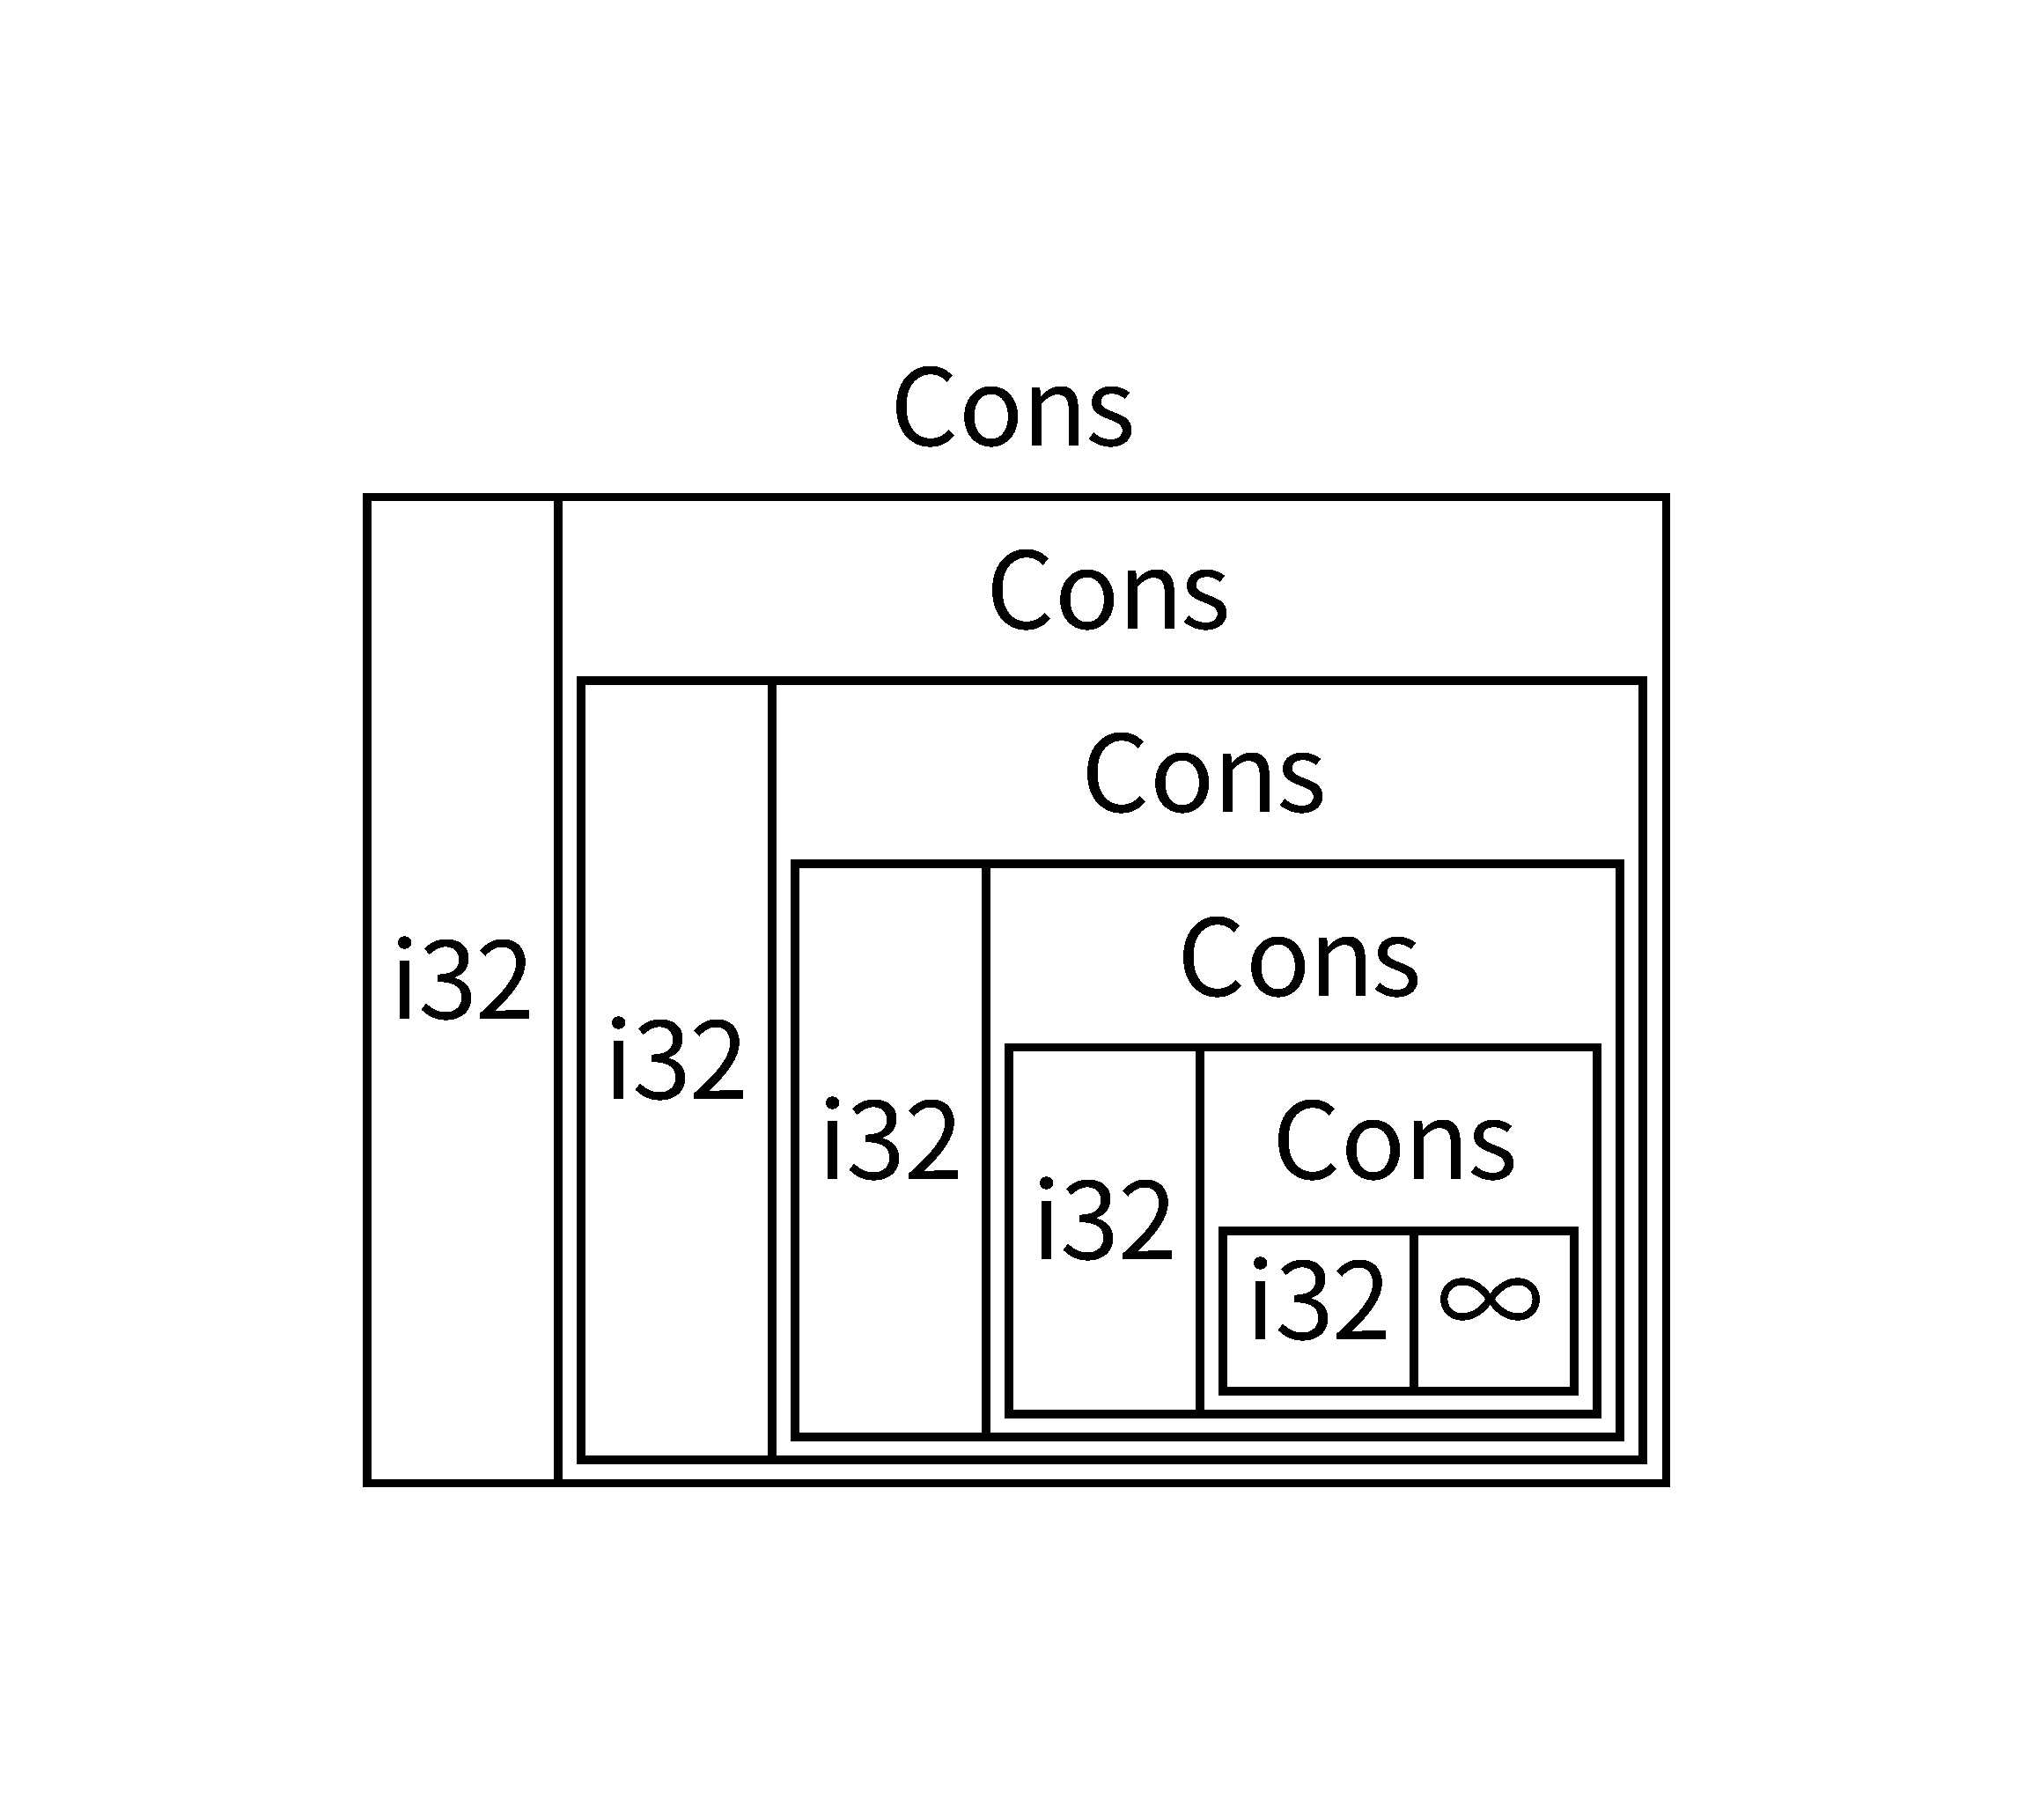
\includegraphics[width=0.5\textwidth,height=\textheight]{img/trpl15-01.pdf}

{Figure 15-1: An infinite \mintinline[]{text}{List} consisting of
infinite \mintinline[]{text}{Cons} variants}

\hypertarget{using-boxt-to-get-a-recursive-type-with-a-known-size}{%
\paragraph{\texorpdfstring{Using \mintinline[]{text}{Box<T>} to Get a
Recursive Type with a Known
Size}{Using  to Get a Recursive Type with a Known Size}}\label{using-boxt-to-get-a-recursive-type-with-a-known-size}}

Rust can't figure out how much space to allocate for recursively defined
types, so the compiler gives the error in Listing 15-4. But the error
does include this helpful suggestion:

\begin{minted}[]{text}
  = help: insert indirection (e.g., a `Box`, `Rc`, or `&`) at some point to
  make `List` representable
\end{minted}

In this suggestion, ``indirection'' means that instead of storing a
value directly, we'll change the data structure to store the value
indirectly by storing a pointer to the value instead.

Because a \mintinline[]{text}{Box<T>} is a pointer, Rust always knows
how much space a \mintinline[]{text}{Box<T>} needs: a pointer's size
doesn't change based on the amount of data it's pointing to. This means
we can put a \mintinline[]{text}{Box<T>} inside the
\mintinline[]{text}{Cons} variant instead of another
\mintinline[]{text}{List} value directly. The
\mintinline[]{text}{Box<T>} will point to the next
\mintinline[]{text}{List} value that will be on the heap rather than
inside the \mintinline[]{text}{Cons} variant. Conceptually, we still
have a list, created with lists ``holding'' other lists, but this
implementation is now more like placing the items next to one another
rather than inside one another.

We can change the definition of the \mintinline[]{text}{List} enum in
Listing 15-2 and the usage of the \mintinline[]{text}{List} in Listing
15-3 to the code in Listing 15-5, which will compile:

{Filename: src/main.rs}

\begin{minted}[]{rust}
enum List {
    Cons(i32, Box<List>),
    Nil,
}

use crate::List::{Cons, Nil};

fn main() {
    let list = Cons(1,
        Box::new(Cons(2,
            Box::new(Cons(3,
                Box::new(Nil))))));
}
\end{minted}

{Listing 15-5: Definition of \mintinline[]{text}{List} that uses
\mintinline[]{text}{Box<T>} in order to have a known size}

The \mintinline[]{text}{Cons} variant will need the size of an
\mintinline[]{text}{i32} plus the space to store the box's pointer data.
The \mintinline[]{text}{Nil} variant stores no values, so it needs less
space than the \mintinline[]{text}{Cons} variant. We now know that any
\mintinline[]{text}{List} value will take up the size of an
\mintinline[]{text}{i32} plus the size of a box's pointer data. By using
a box, we've broken the infinite, recursive chain, so the compiler can
figure out the size it needs to store a \mintinline[]{text}{List} value.
Figure 15-2 shows what the \mintinline[]{text}{Cons} variant looks like
now.

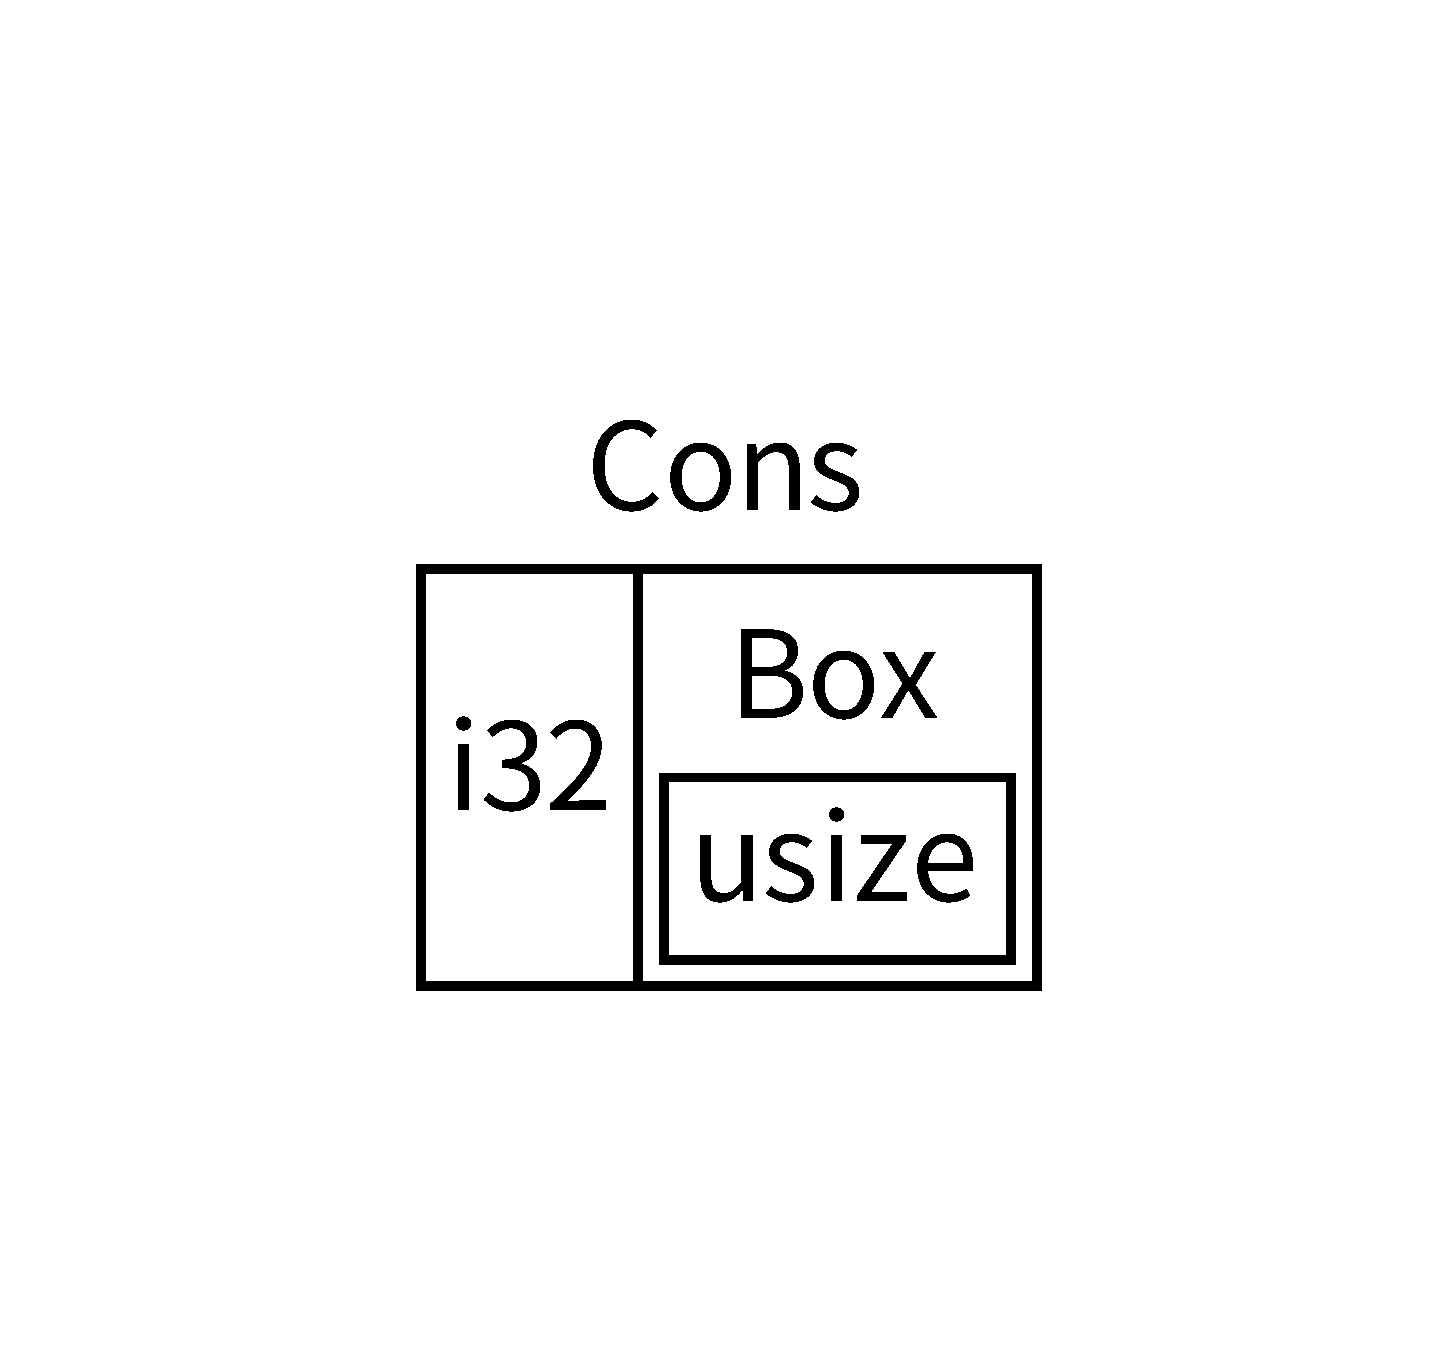
\includegraphics{img/trpl15-02.pdf}

{Figure 15-2: A \mintinline[]{text}{List} that is not infinitely sized
because \mintinline[]{text}{Cons} holds a \mintinline[]{text}{Box}}

Boxes provide only the indirection and heap allocation; they don't have
any other special capabilities, like those we'll see with the other
smart pointer types. They also don't have any performance overhead that
these special capabilities incur, so they can be useful in cases like
the cons list where the indirection is the only feature we need. We'll
look at more use cases for boxes in Chapter 17, too.

The \mintinline[]{text}{Box<T>} type is a smart pointer because it
implements the \mintinline[]{text}{Deref} trait, which allows
\mintinline[]{text}{Box<T>} values to be treated like references. When a
\mintinline[]{text}{Box<T>} value goes out of scope, the heap data that
the box is pointing to is cleaned up as well because of the
\mintinline[]{text}{Drop} trait implementation. Let's explore these two
traits in more detail. These two traits will be even more important to
the functionality provided by the other smart pointer types we'll
discuss in the rest of this chapter.

\hypertarget{treating-smart-pointers-like-regular-references-with-the-deref-trait}{%
\subsection{\texorpdfstring{Treating Smart Pointers Like Regular
References with the \mintinline[]{text}{Deref}
Trait}{Treating Smart Pointers Like Regular References with the  Trait}}\label{treating-smart-pointers-like-regular-references-with-the-deref-trait}}

Implementing the \mintinline[]{text}{Deref} trait allows you to
customize the behavior of the \emph{dereference operator},
\mintinline[]{text}{*} (as opposed to the multiplication or glob
operator). By implementing \mintinline[]{text}{Deref} in such a way that
a smart pointer can be treated like a regular reference, you can write
code that operates on references and use that code with smart pointers
too.

Let's first look at how the dereference operator works with regular
references. Then we'll try to define a custom type that behaves like
\mintinline[]{text}{Box<T>}, and see why the dereference operator
doesn't work like a reference on our newly defined type. We'll explore
how implementing the \mintinline[]{text}{Deref} trait makes it possible
for smart pointers to work in ways similar to references. Then we'll
look at Rust's \emph{deref coercion} feature and how it lets us work
with either references or smart pointers.

\begin{quote}
Note: there's one big difference between the
\mintinline[]{text}{MyBox<T>} type we're about to build and the real
\mintinline[]{text}{Box<T>}: our version will not store its data on the
heap. We are focusing this example on \mintinline[]{text}{Deref}, so
where the data is actually stored is less important than the
pointer-like behavior.
\end{quote}

\hypertarget{following-the-pointer-to-the-value-with-the-dereference-operator}{%
\subsubsection{Following the Pointer to the Value with the Dereference
Operator}\label{following-the-pointer-to-the-value-with-the-dereference-operator}}

A regular reference is a type of pointer, and one way to think of a
pointer is as an arrow to a value stored somewhere else. In Listing
15-6, we create a reference to an \mintinline[]{text}{i32} value and
then use the dereference operator to follow the reference to the data:

{Filename: src/main.rs}

\begin{minted}[]{rust}
fn main() {
    let x = 5;
    let y = &x;

    assert_eq!(5, x);
    assert_eq!(5, *y);
}
\end{minted}

{Listing 15-6: Using the dereference operator to follow a reference to
an \mintinline[]{text}{i32} value}

The variable \mintinline[]{text}{x} holds an \mintinline[]{text}{i32}
value, \mintinline[]{text}{5}. We set \mintinline[]{text}{y} equal to a
reference to \mintinline[]{text}{x}. We can assert that
\mintinline[]{text}{x} is equal to \mintinline[]{text}{5}. However, if
we want to make an assertion about the value in \mintinline[]{text}{y},
we have to use \mintinline[]{text}{*y} to follow the reference to the
value it's pointing to (hence \emph{dereference}). Once we dereference
\mintinline[]{text}{y}, we have access to the integer value
\mintinline[]{text}{y} is pointing to that we can compare with
\mintinline[]{text}{5}.

If we tried to write \mintinline[]{text}{assert_eq!(5, y);} instead, we
would get this compilation error:

\begin{minted}[]{text}
error[E0277]: can't compare `{integer}` with `&{integer}`
 --> src/main.rs:6:5
  |
6 |     assert_eq!(5, y);
  |     ^^^^^^^^^^^^^^^^^ no implementation for `{integer} == &{integer}`
  |
  = help: the trait `std::cmp::PartialEq<&{integer}>` is not implemented for
  `{integer}`
\end{minted}

Comparing a number and a reference to a number isn't allowed because
they're different types. We must use the dereference operator to follow
the reference to the value it's pointing to.

\hypertarget{using-boxt-like-a-reference}{%
\subsubsection{\texorpdfstring{Using \mintinline[]{text}{Box<T>} Like a
Reference}{Using  Like a Reference}}\label{using-boxt-like-a-reference}}

We can rewrite the code in Listing 15-6 to use a
\mintinline[]{text}{Box<T>} instead of a reference; the dereference
operator will work as shown in Listing 15-7:

{Filename: src/main.rs}

\begin{minted}[]{rust}
fn main() {
    let x = 5;
    let y = Box::new(x);

    assert_eq!(5, x);
    assert_eq!(5, *y);
}
\end{minted}

{Listing 15-7: Using the dereference operator on a
\mintinline[]{text}{Box<i32>}}

The only difference between Listing 15-7 and Listing 15-6 is that here
we set \mintinline[]{text}{y} to be an instance of a box pointing to the
value in \mintinline[]{text}{x} rather than a reference pointing to the
value of \mintinline[]{text}{x}. In the last assertion, we can use the
dereference operator to follow the box's pointer in the same way that we
did when \mintinline[]{text}{y} was a reference. Next, we'll explore
what is special about \mintinline[]{text}{Box<T>} that enables us to use
the dereference operator by defining our own box type.

\hypertarget{defining-our-own-smart-pointer}{%
\subsubsection{Defining Our Own Smart
Pointer}\label{defining-our-own-smart-pointer}}

Let's build a smart pointer similar to the \mintinline[]{text}{Box<T>}
type provided by the standard library to experience how smart pointers
behave differently from references by default. Then we'll look at how to
add the ability to use the dereference operator.

The \mintinline[]{text}{Box<T>} type is ultimately defined as a tuple
struct with one element, so Listing 15-8 defines a
\mintinline[]{text}{MyBox<T>} type in the same way. We'll also define a
\mintinline[]{text}{new} function to match the \mintinline[]{text}{new}
function defined on \mintinline[]{text}{Box<T>}.

{Filename: src/main.rs}

\begin{minted}[]{rust}
struct MyBox<T>(T);

impl<T> MyBox<T> {
    fn new(x: T) -> MyBox<T> {
        MyBox(x)
    }
}
\end{minted}

{Listing 15-8: Defining a \mintinline[]{text}{MyBox<T>} type}

We define a struct named \mintinline[]{text}{MyBox} and declare a
generic parameter \mintinline[]{text}{T}, because we want our type to
hold values of any type. The \mintinline[]{text}{MyBox} type is a tuple
struct with one element of type \mintinline[]{text}{T}. The
\mintinline[]{text}{MyBox::new} function takes one parameter of type
\mintinline[]{text}{T} and returns a \mintinline[]{text}{MyBox} instance
that holds the value passed in.

Let's try adding the \mintinline[]{text}{main} function in Listing 15-7
to Listing 15-8 and changing it to use the \mintinline[]{text}{MyBox<T>}
type we've defined instead of \mintinline[]{text}{Box<T>}. The code in
Listing 15-9 won't compile because Rust doesn't know how to dereference
\mintinline[]{text}{MyBox}.

{Filename: src/main.rs}

\begin{minted}[]{rust}
fn main() {
    let x = 5;
    let y = MyBox::new(x);

    assert_eq!(5, x);
    assert_eq!(5, *y);
}
\end{minted}

{Listing 15-9: Attempting to use \mintinline[]{text}{MyBox<T>} in the
same way we used references and \mintinline[]{text}{Box<T>}}

Here's the resulting compilation error:

\begin{minted}[]{text}
error[E0614]: type `MyBox<{integer}>` cannot be dereferenced
  --> src/main.rs:14:19
   |
14 |     assert_eq!(5, *y);
   |                   ^^
\end{minted}

Our \mintinline[]{text}{MyBox<T>} type can't be dereferenced because we
haven't implemented that ability on our type. To enable dereferencing
with the \mintinline[]{text}{*} operator, we implement the
\mintinline[]{text}{Deref} trait.

\hypertarget{treating-a-type-like-a-reference-by-implementing-the-deref-trait}{%
\subsubsection{\texorpdfstring{Treating a Type Like a Reference by
Implementing the \mintinline[]{text}{Deref}
Trait}{Treating a Type Like a Reference by Implementing the  Trait}}\label{treating-a-type-like-a-reference-by-implementing-the-deref-trait}}

As discussed in Chapter 10, to implement a trait, we need to provide
implementations for the trait's required methods. The
\mintinline[]{text}{Deref} trait, provided by the standard library,
requires us to implement one method named \mintinline[]{text}{deref}
that borrows \mintinline[]{text}{self} and returns a reference to the
inner data. Listing 15-10 contains an implementation of
\mintinline[]{text}{Deref} to add to the definition of
\mintinline[]{text}{MyBox}:

{Filename: src/main.rs}

\begin{minted}[]{rust}
use std::ops::Deref;

# struct MyBox<T>(T);
impl<T> Deref for MyBox<T> {
    type Target = T;

    fn deref(&self) -> &T {
        &self.0
    }
}
\end{minted}

{Listing 15-10: Implementing \mintinline[]{text}{Deref} on
\mintinline[]{text}{MyBox<T>}}

The \mintinline[]{text}{type Target = T;} syntax defines an associated
type for the \mintinline[]{text}{Deref} trait to use. Associated types
are a slightly different way of declaring a generic parameter, but you
don't need to worry about them for now; we'll cover them in more detail
in Chapter 19.

We fill in the body of the \mintinline[]{text}{deref} method with
\mintinline[]{text}{&self.0} so \mintinline[]{text}{deref} returns a
reference to the value we want to access with the \mintinline[]{text}{*}
operator. The \mintinline[]{text}{main} function in Listing 15-9 that
calls \mintinline[]{text}{*} on the \mintinline[]{text}{MyBox<T>} value
now compiles, and the assertions pass!

Without the \mintinline[]{text}{Deref} trait, the compiler can only
dereference \mintinline[]{text}{&} references. The
\mintinline[]{text}{deref} method gives the compiler the ability to take
a value of any type that implements \mintinline[]{text}{Deref} and call
the \mintinline[]{text}{deref} method to get a \mintinline[]{text}{&}
reference that it knows how to dereference.

When we entered \mintinline[]{text}{*y} in Listing 15-9, behind the
scenes Rust actually ran this code:

\begin{minted}[]{rust}
*(y.deref())
\end{minted}

Rust substitutes the \mintinline[]{text}{*} operator with a call to the
\mintinline[]{text}{deref} method and then a plain dereference so we
don't have to think about whether or not we need to call the
\mintinline[]{text}{deref} method. This Rust feature lets us write code
that functions identically whether we have a regular reference or a type
that implements \mintinline[]{text}{Deref}.

The reason the \mintinline[]{text}{deref} method returns a reference to
a value, and that the plain dereference outside the parentheses in
\mintinline[]{text}{*(y.deref())} is still necessary, is the ownership
system. If the \mintinline[]{text}{deref} method returned the value
directly instead of a reference to the value, the value would be moved
out of \mintinline[]{text}{self}. We don't want to take ownership of the
inner value inside \mintinline[]{text}{MyBox<T>} in this case or in most
cases where we use the dereference operator.

Note that the \mintinline[]{text}{*} operator is replaced with a call to
the \mintinline[]{text}{deref} method and then a call to the
\mintinline[]{text}{*} operator just once, each time we use a
\mintinline[]{text}{*} in our code. Because the substitution of the
\mintinline[]{text}{*} operator does not recurse infinitely, we end up
with data of type \mintinline[]{text}{i32}, which matches the
\mintinline[]{text}{5} in \mintinline[]{text}{assert_eq!} in Listing
15-9.

\hypertarget{implicit-deref-coercions-with-functions-and-methods}{%
\subsubsection{Implicit Deref Coercions with Functions and
Methods}\label{implicit-deref-coercions-with-functions-and-methods}}

\emph{Deref coercion} is a convenience that Rust performs on arguments
to functions and methods. Deref coercion converts a reference to a type
that implements \mintinline[]{text}{Deref} into a reference to a type
that \mintinline[]{text}{Deref} can convert the original type into.
Deref coercion happens automatically when we pass a reference to a
particular type's value as an argument to a function or method that
doesn't match the parameter type in the function or method definition. A
sequence of calls to the \mintinline[]{text}{deref} method converts the
type we provided into the type the parameter needs.

Deref coercion was added to Rust so that programmers writing function
and method calls don't need to add as many explicit references and
dereferences with \mintinline[]{text}{&} and \mintinline[]{text}{*}. The
deref coercion feature also lets us write more code that can work for
either references or smart pointers.

To see deref coercion in action, let's use the
\mintinline[]{text}{MyBox<T>} type we defined in Listing 15-8 as well as
the implementation of \mintinline[]{text}{Deref} that we added in
Listing 15-10. Listing 15-11 shows the definition of a function that has
a string slice parameter:

{Filename: src/main.rs}

\begin{minted}[]{rust}
fn hello(name: &str) {
    println!("Hello, {}!", name);
}
\end{minted}

{Listing 15-11: A \mintinline[]{text}{hello} function that has the
parameter \mintinline[]{text}{name} of type \mintinline[]{text}{&str}}

We can call the \mintinline[]{text}{hello} function with a string slice
as an argument, such as \mintinline[]{text}{hello("Rust");} for example.
Deref coercion makes it possible to call \mintinline[]{text}{hello} with
a reference to a value of type \mintinline[]{text}{MyBox<String>}, as
shown in Listing 15-12:

{Filename: src/main.rs}

\begin{minted}[]{rust}
# use std::ops::Deref;
#
# struct MyBox<T>(T);
#
# impl<T> MyBox<T> {
#     fn new(x: T) -> MyBox<T> {
#         MyBox(x)
#     }
# }
#
# impl<T> Deref for MyBox<T> {
#     type Target = T;
#
#     fn deref(&self) -> &T {
#         &self.0
#     }
# }
#
# fn hello(name: &str) {
#     println!("Hello, {}!", name);
# }
#
fn main() {
    let m = MyBox::new(String::from("Rust"));
    hello(&m);
}
\end{minted}

{Listing 15-12: Calling \mintinline[]{text}{hello} with a reference to a
\mintinline[]{text}{MyBox<String>} value, which works because of deref
coercion}

Here we're calling the \mintinline[]{text}{hello} function with the
argument \mintinline[]{text}{&m}, which is a reference to a
\mintinline[]{text}{MyBox<String>} value. Because we implemented the
\mintinline[]{text}{Deref} trait on \mintinline[]{text}{MyBox<T>} in
Listing 15-10, Rust can turn \mintinline[]{text}{&MyBox<String>} into
\mintinline[]{text}{&String} by calling \mintinline[]{text}{deref}. The
standard library provides an implementation of
\mintinline[]{text}{Deref} on \mintinline[]{text}{String} that returns a
string slice, and this is in the API documentation for
\mintinline[]{text}{Deref}. Rust calls \mintinline[]{text}{deref} again
to turn the \mintinline[]{text}{&String} into \mintinline[]{text}{&str},
which matches the \mintinline[]{text}{hello} function's definition.

If Rust didn't implement deref coercion, we would have to write the code
in Listing 15-13 instead of the code in Listing 15-12 to call
\mintinline[]{text}{hello} with a value of type
\mintinline[]{text}{&MyBox<String>}.

{Filename: src/main.rs}

\begin{minted}[]{rust}
# use std::ops::Deref;
#
# struct MyBox<T>(T);
#
# impl<T> MyBox<T> {
#     fn new(x: T) -> MyBox<T> {
#         MyBox(x)
#     }
# }
#
# impl<T> Deref for MyBox<T> {
#     type Target = T;
#
#     fn deref(&self) -> &T {
#         &self.0
#     }
# }
#
# fn hello(name: &str) {
#     println!("Hello, {}!", name);
# }
#
fn main() {
    let m = MyBox::new(String::from("Rust"));
    hello(&(*m)[..]);
}
\end{minted}

{Listing 15-13: The code we would have to write if Rust didn't have
deref coercion}

The \mintinline[]{text}{(*m)} dereferences the
\mintinline[]{text}{MyBox<String>} into a \mintinline[]{text}{String}.
Then the \mintinline[]{text}{&} and \mintinline[]{text}{[..]} take a
string slice of the \mintinline[]{text}{String} that is equal to the
whole string to match the signature of \mintinline[]{text}{hello}. The
code without deref coercions is harder to read, write, and understand
with all of these symbols involved. Deref coercion allows Rust to handle
these conversions for us automatically.

When the \mintinline[]{text}{Deref} trait is defined for the types
involved, Rust will analyze the types and use
\mintinline[]{text}{Deref::deref} as many times as necessary to get a
reference to match the parameter's type. The number of times that
\mintinline[]{text}{Deref::deref} needs to be inserted is resolved at
compile time, so there is no runtime penalty for taking advantage of
deref coercion!

\hypertarget{how-deref-coercion-interacts-with-mutability}{%
\subsubsection{How Deref Coercion Interacts with
Mutability}\label{how-deref-coercion-interacts-with-mutability}}

Similar to how you use the \mintinline[]{text}{Deref} trait to override
the \mintinline[]{text}{*} operator on immutable references, you can use
the \mintinline[]{text}{DerefMut} trait to override the
\mintinline[]{text}{*} operator on mutable references.

Rust does deref coercion when it finds types and trait implementations
in three cases:

\begin{itemize}
\tightlist
\item
  From \mintinline[]{text}{&T} to \mintinline[]{text}{&U} when
  \mintinline[]{text}{T: Deref<Target=U>}
\item
  From \mintinline[]{text}{&mut T} to \mintinline[]{text}{&mut U} when
  \mintinline[]{text}{T: DerefMut<Target=U>}
\item
  From \mintinline[]{text}{&mut T} to \mintinline[]{text}{&U} when
  \mintinline[]{text}{T: Deref<Target=U>}
\end{itemize}

The first two cases are the same except for mutability. The first case
states that if you have a \mintinline[]{text}{&T}, and
\mintinline[]{text}{T} implements \mintinline[]{text}{Deref} to some
type \mintinline[]{text}{U}, you can get a \mintinline[]{text}{&U}
transparently. The second case states that the same deref coercion
happens for mutable references.

The third case is trickier: Rust will also coerce a mutable reference to
an immutable one. But the reverse is \emph{not} possible: immutable
references will never coerce to mutable references. Because of the
borrowing rules, if you have a mutable reference, that mutable reference
must be the only reference to that data (otherwise, the program wouldn't
compile). Converting one mutable reference to one immutable reference
will never break the borrowing rules. Converting an immutable reference
to a mutable reference would require that there is only one immutable
reference to that data, and the borrowing rules don't guarantee that.
Therefore, Rust can't make the assumption that converting an immutable
reference to a mutable reference is possible.

\hypertarget{running-code-on-cleanup-with-the-drop-trait}{%
\subsection{\texorpdfstring{Running Code on Cleanup with the
\mintinline[]{text}{Drop}
Trait}{Running Code on Cleanup with the  Trait}}\label{running-code-on-cleanup-with-the-drop-trait}}

The second trait important to the smart pointer pattern is
\mintinline[]{text}{Drop}, which lets you customize what happens when a
value is about to go out of scope. You can provide an implementation for
the \mintinline[]{text}{Drop} trait on any type, and the code you
specify can be used to release resources like files or network
connections. We're introducing \mintinline[]{text}{Drop} in the context
of smart pointers because the functionality of the
\mintinline[]{text}{Drop} trait is almost always used when implementing
a smart pointer. For example, \mintinline[]{text}{Box<T>} customizes
\mintinline[]{text}{Drop} to deallocate the space on the heap that the
box points to.

In some languages, the programmer must call code to free memory or
resources every time they finish using an instance of a smart pointer.
If they forget, the system might become overloaded and crash. In Rust,
you can specify that a particular bit of code be run whenever a value
goes out of scope, and the compiler will insert this code automatically.
As a result, you don't need to be careful about placing cleanup code
everywhere in a program that an instance of a particular type is
finished with---you still won't leak resources!

Specify the code to run when a value goes out of scope by implementing
the \mintinline[]{text}{Drop} trait. The \mintinline[]{text}{Drop} trait
requires you to implement one method named \mintinline[]{text}{drop}
that takes a mutable reference to \mintinline[]{text}{self}. To see when
Rust calls \mintinline[]{text}{drop}, let's implement
\mintinline[]{text}{drop} with \mintinline[]{text}{println!} statements
for now.

Listing 15-14 shows a \mintinline[]{text}{CustomSmartPointer} struct
whose only custom functionality is that it will print
\mintinline[]{text}{Dropping CustomSmartPointer!} when the instance goes
out of scope. This example demonstrates when Rust runs the
\mintinline[]{text}{drop} function.

{Filename: src/main.rs}

\begin{minted}[]{rust}
struct CustomSmartPointer {
    data: String,
}

impl Drop for CustomSmartPointer {
    fn drop(&mut self) {
        println!("Dropping CustomSmartPointer with data `{}`!", self.data);
    }
}

fn main() {
    let c = CustomSmartPointer { data: String::from("my stuff") };
    let d = CustomSmartPointer { data: String::from("other stuff") };
    println!("CustomSmartPointers created.");
}
\end{minted}

{Listing 15-14: A \mintinline[]{text}{CustomSmartPointer} struct that
implements the \mintinline[]{text}{Drop} trait where we would put our
cleanup code}

The \mintinline[]{text}{Drop} trait is included in the prelude, so we
don't need to bring it into scope. We implement the
\mintinline[]{text}{Drop} trait on
\mintinline[]{text}{CustomSmartPointer} and provide an implementation
for the \mintinline[]{text}{drop} method that calls
\mintinline[]{text}{println!}. The body of the \mintinline[]{text}{drop}
function is where you would place any logic that you wanted to run when
an instance of your type goes out of scope. We're printing some text
here to demonstrate when Rust will call \mintinline[]{text}{drop}.

In \mintinline[]{text}{main}, we create two instances of
\mintinline[]{text}{CustomSmartPointer} and then print
\mintinline[]{text}{CustomSmartPointers created.}. At the end of
\mintinline[]{text}{main}, our instances of
\mintinline[]{text}{CustomSmartPointer} will go out of scope, and Rust
will call the code we put in the \mintinline[]{text}{drop} method,
printing our final message. Note that we didn't need to call the
\mintinline[]{text}{drop} method explicitly.

When we run this program, we'll see the following output:

\begin{minted}[]{text}
CustomSmartPointers created.
Dropping CustomSmartPointer with data `other stuff`!
Dropping CustomSmartPointer with data `my stuff`!
\end{minted}

Rust automatically called \mintinline[]{text}{drop} for us when our
instances went out of scope, calling the code we specified. Variables
are dropped in the reverse order of their creation, so
\mintinline[]{text}{d} was dropped before \mintinline[]{text}{c}. This
example gives you a visual guide to how the \mintinline[]{text}{drop}
method works; usually you would specify the cleanup code that your type
needs to run rather than a print message.

\hypertarget{dropping-a-value-early-with-stdmemdrop}{%
\subsubsection{\texorpdfstring{Dropping a Value Early with
\mintinline[]{text}{std::mem::drop}}{Dropping a Value Early with }}\label{dropping-a-value-early-with-stdmemdrop}}

Unfortunately, it's not straightforward to disable the automatic
\mintinline[]{text}{drop} functionality. Disabling
\mintinline[]{text}{drop} isn't usually necessary; the whole point of
the \mintinline[]{text}{Drop} trait is that it's taken care of
automatically. Occasionally, however, you might want to clean up a value
early. One example is when using smart pointers that manage locks: you
might want to force the \mintinline[]{text}{drop} method that releases
the lock to run so other code in the same scope can acquire the lock.
Rust doesn't let you call the \mintinline[]{text}{Drop} trait's
\mintinline[]{text}{drop} method manually; instead you have to call the
\mintinline[]{text}{std::mem::drop} function provided by the standard
library if you want to force a value to be dropped before the end of its
scope.

If we try to call the \mintinline[]{text}{Drop} trait's
\mintinline[]{text}{drop} method manually by modifying the
\mintinline[]{text}{main} function from Listing 15-14, as shown in
Listing 15-15, we'll get a compiler error:

{Filename: src/main.rs}

\begin{minted}[]{rust}
fn main() {
    let c = CustomSmartPointer { data: String::from("some data") };
    println!("CustomSmartPointer created.");
    c.drop();
    println!("CustomSmartPointer dropped before the end of main.");
}
\end{minted}

{Listing 15-15: Attempting to call the \mintinline[]{text}{drop} method
from the \mintinline[]{text}{Drop} trait manually to clean up early}

When we try to compile this code, we'll get this error:

\begin{minted}[]{text}
error[E0040]: explicit use of destructor method
  --> src/main.rs:14:7
   |
14 |     c.drop();
   |       ^^^^ explicit destructor calls not allowed
\end{minted}

This error message states that we're not allowed to explicitly call
\mintinline[]{text}{drop}. The error message uses the term
\emph{destructor}, which is the general programming term for a function
that cleans up an instance. A \emph{destructor} is analogous to a
\emph{constructor}, which creates an instance. The
\mintinline[]{text}{drop} function in Rust is one particular destructor.

Rust doesn't let us call \mintinline[]{text}{drop} explicitly because
Rust would still automatically call \mintinline[]{text}{drop} on the
value at the end of \mintinline[]{text}{main}. This would be a
\emph{double free} error because Rust would be trying to clean up the
same value twice.

We can't disable the automatic insertion of \mintinline[]{text}{drop}
when a value goes out of scope, and we can't call the
\mintinline[]{text}{drop} method explicitly. So, if we need to force a
value to be cleaned up early, we can use the
\mintinline[]{text}{std::mem::drop} function.

The \mintinline[]{text}{std::mem::drop} function is different from the
\mintinline[]{text}{drop} method in the \mintinline[]{text}{Drop} trait.
We call it by passing the value we want to force to be dropped early as
an argument. The function is in the prelude, so we can modify
\mintinline[]{text}{main} in Listing 15-15 to call the
\mintinline[]{text}{drop} function, as shown in Listing 15-16:

{Filename: src/main.rs}

\begin{minted}[]{rust}
# struct CustomSmartPointer {
#     data: String,
# }
#
# impl Drop for CustomSmartPointer {
#     fn drop(&mut self) {
#         println!("Dropping CustomSmartPointer!");
#     }
# }
#
fn main() {
    let c = CustomSmartPointer { data: String::from("some data") };
    println!("CustomSmartPointer created.");
    drop(c);
    println!("CustomSmartPointer dropped before the end of main.");
}
\end{minted}

{Listing 15-16: Calling \mintinline[]{text}{std::mem::drop} to
explicitly drop a value before it goes out of scope}

Running this code will print the following:

\begin{minted}[]{text}
CustomSmartPointer created.
Dropping CustomSmartPointer with data `some data`!
CustomSmartPointer dropped before the end of main.
\end{minted}

The text
\mintinline[]{text}{Dropping CustomSmartPointer with data `some data`!}
is printed between the \mintinline[]{text}{CustomSmartPointer created.}
and
\mintinline[]{text}{CustomSmartPointer dropped before the end of main.}
text, showing that the \mintinline[]{text}{drop} method code is called
to drop \mintinline[]{text}{c} at that point.

You can use code specified in a \mintinline[]{text}{Drop} trait
implementation in many ways to make cleanup convenient and safe: for
instance, you could use it to create your own memory allocator! With the
\mintinline[]{text}{Drop} trait and Rust's ownership system, you don't
have to remember to clean up because Rust does it automatically.

You also don't have to worry about problems resulting from accidentally
cleaning up values still in use: the ownership system that makes sure
references are always valid also ensures that \mintinline[]{text}{drop}
gets called only once when the value is no longer being used.

Now that we've examined \mintinline[]{text}{Box<T>} and some of the
characteristics of smart pointers, let's look at a few other smart
pointers defined in the standard library.

\hypertarget{rct-the-reference-counted-smart-pointer}{%
\subsection{\texorpdfstring{\mintinline[]{text}{Rc<T>}, the Reference
Counted Smart
Pointer}{, the Reference Counted Smart Pointer}}\label{rct-the-reference-counted-smart-pointer}}

In the majority of cases, ownership is clear: you know exactly which
variable owns a given value. However, there are cases when a single
value might have multiple owners. For example, in graph data structures,
multiple edges might point to the same node, and that node is
conceptually owned by all of the edges that point to it. A node
shouldn't be cleaned up unless it doesn't have any edges pointing to it.

To enable multiple ownership, Rust has a type called
\mintinline[]{text}{Rc<T>}, which is an abbreviation for \emph{reference
counting}. The \mintinline[]{text}{Rc<T>} type keeps track of the number
of references to a value which determines whether or not a value is
still in use. If there are zero references to a value, the value can be
cleaned up without any references becoming invalid.

Imagine \mintinline[]{text}{Rc<T>} as a TV in a family room. When one
person enters to watch TV, they turn it on. Others can come into the
room and watch the TV. When the last person leaves the room, they turn
off the TV because it's no longer being used. If someone turns off the
TV while others are still watching it, there would be uproar from the
remaining TV watchers!

We use the \mintinline[]{text}{Rc<T>} type when we want to allocate some
data on the heap for multiple parts of our program to read and we can't
determine at compile time which part will finish using the data last. If
we knew which part would finish last, we could just make that part the
data's owner, and the normal ownership rules enforced at compile time
would take effect.

Note that \mintinline[]{text}{Rc<T>} is only for use in single-threaded
scenarios. When we discuss concurrency in Chapter 16, we'll cover how to
do reference counting in multithreaded programs.

\hypertarget{using-rct-to-share-data}{%
\subsubsection{\texorpdfstring{Using \mintinline[]{text}{Rc<T>} to Share
Data}{Using  to Share Data}}\label{using-rct-to-share-data}}

Let's return to our cons list example in Listing 15-5. Recall that we
defined it using \mintinline[]{text}{Box<T>}. This time, we'll create
two lists that both share ownership of a third list. Conceptually, this
looks similar to Figure 15-3:

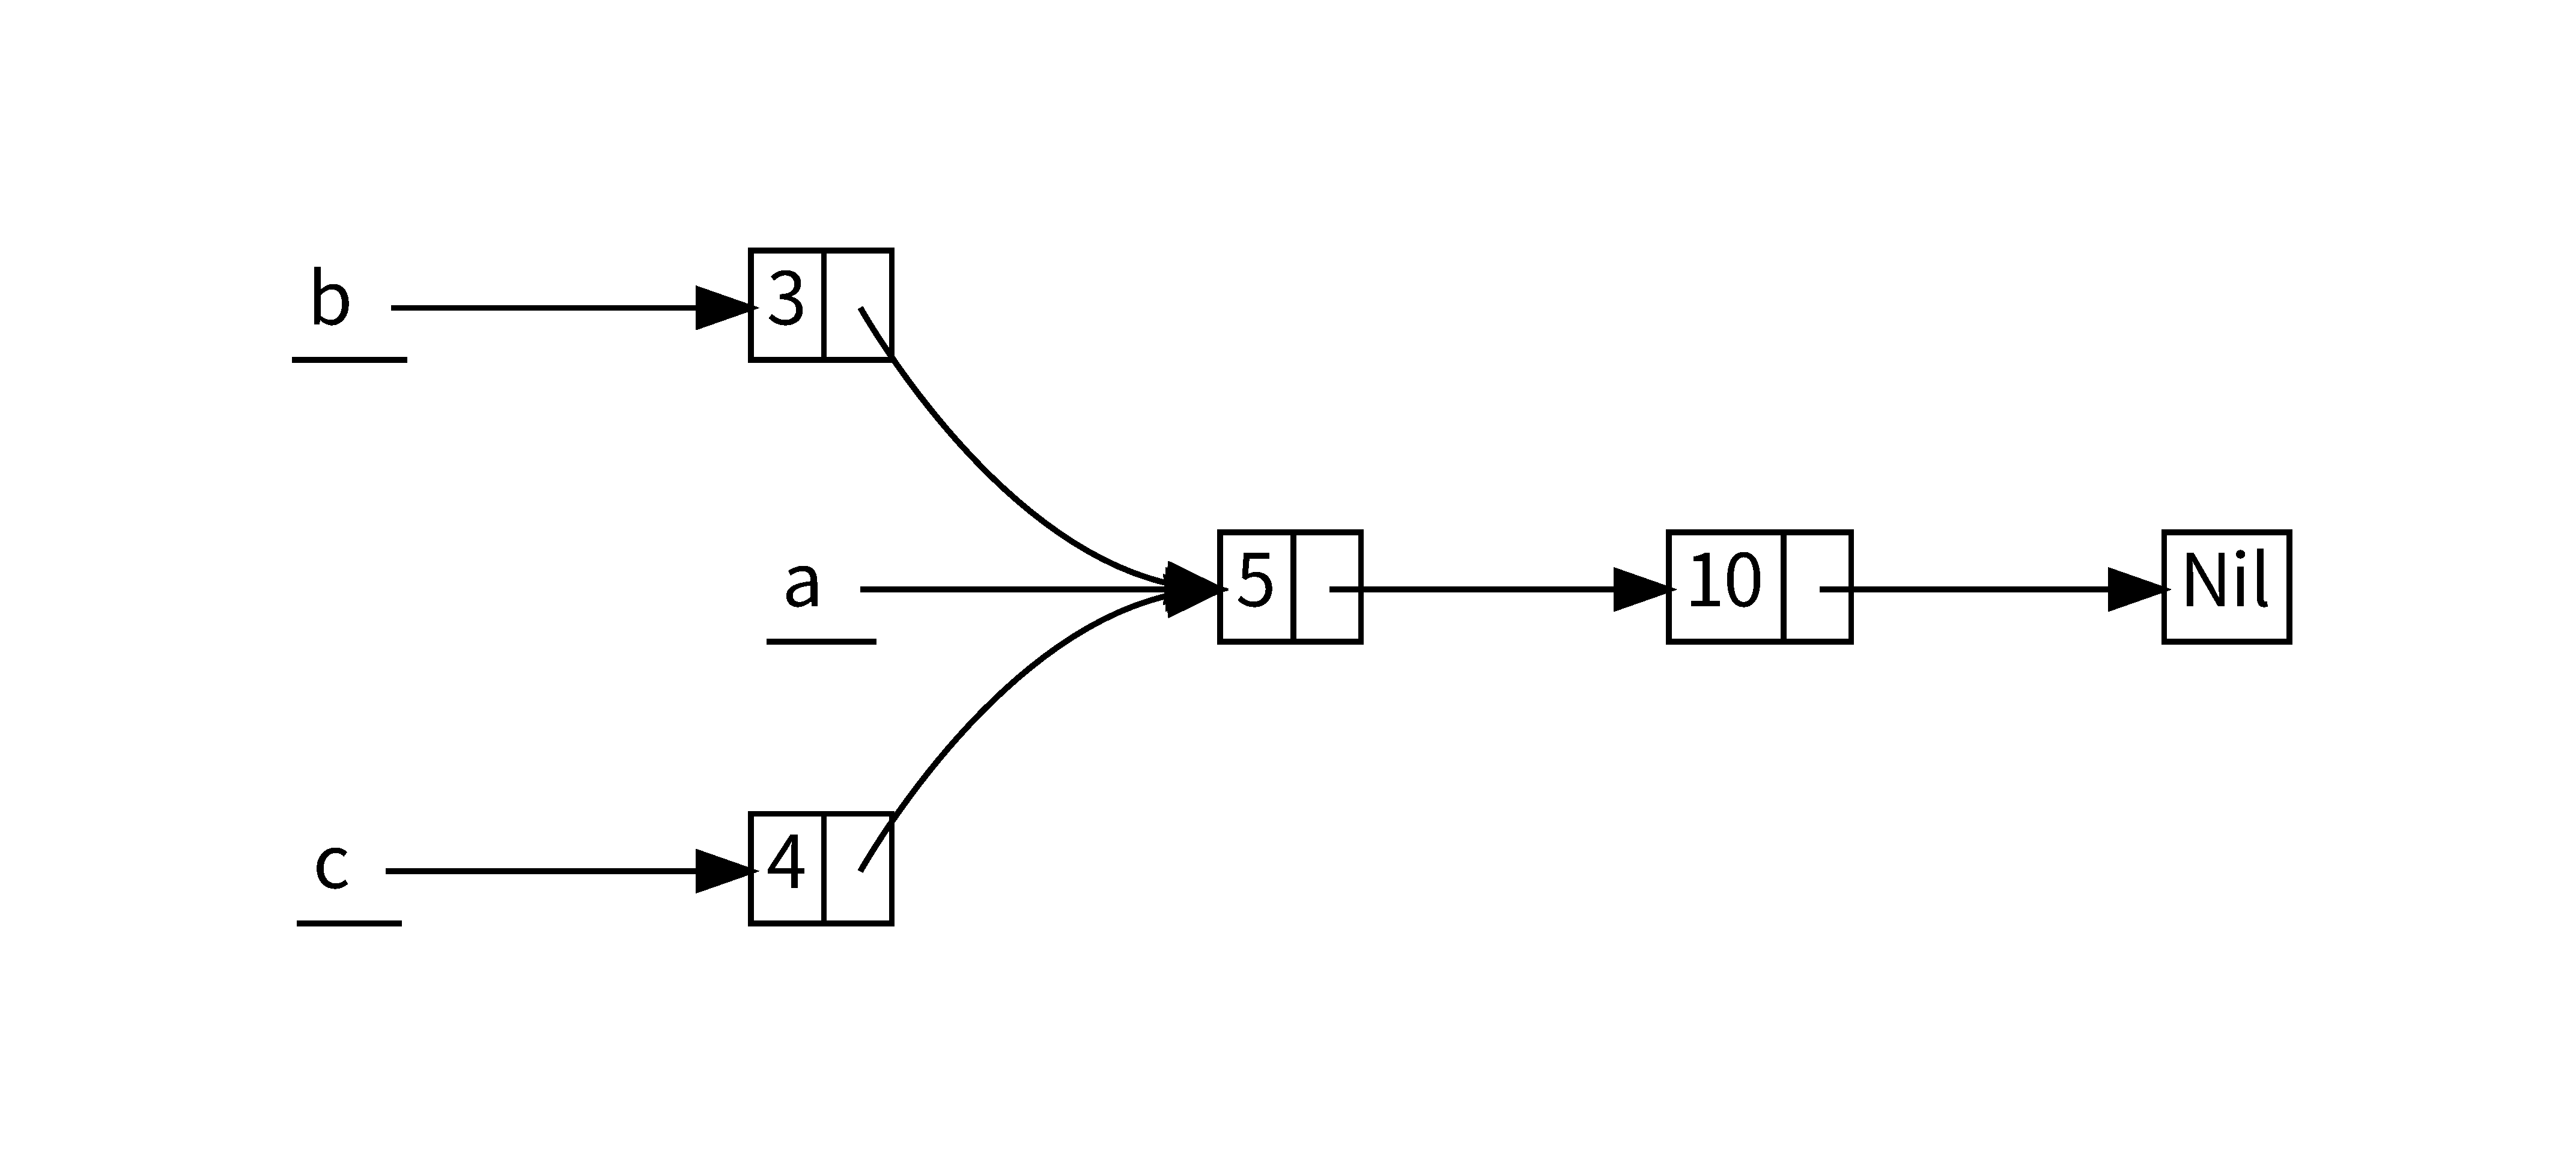
\includegraphics{img/trpl15-03.pdf}

{Figure 15-3: Two lists, \mintinline[]{text}{b} and
\mintinline[]{text}{c}, sharing ownership of a third list,
\mintinline[]{text}{a}}

We'll create list \mintinline[]{text}{a} that contains 5 and then 10.
Then we'll make two more lists: \mintinline[]{text}{b} that starts with
3 and \mintinline[]{text}{c} that starts with 4. Both
\mintinline[]{text}{b} and \mintinline[]{text}{c} lists will then
continue on to the first \mintinline[]{text}{a} list containing 5 and
10. In other words, both lists will share the first list containing 5
and 10.

Trying to implement this scenario using our definition of
\mintinline[]{text}{List} with \mintinline[]{text}{Box<T>} won't work,
as shown in Listing 15-17:

{Filename: src/main.rs}

\begin{minted}[]{rust}
enum List {
    Cons(i32, Box<List>),
    Nil,
}

use crate::List::{Cons, Nil};

fn main() {
    let a = Cons(5,
        Box::new(Cons(10,
            Box::new(Nil))));
    let b = Cons(3, Box::new(a));
    let c = Cons(4, Box::new(a));
}
\end{minted}

{Listing 15-17: Demonstrating we're not allowed to have two lists using
\mintinline[]{text}{Box<T>} that try to share ownership of a third list}

When we compile this code, we get this error:

\begin{minted}[]{text}
error[E0382]: use of moved value: `a`
  --> src/main.rs:13:30
   |
12 |     let b = Cons(3, Box::new(a));
   |                              - value moved here
13 |     let c = Cons(4, Box::new(a));
   |                              ^ value used here after move
   |
   = note: move occurs because `a` has type `List`, which does not implement
   the `Copy` trait
\end{minted}

The \mintinline[]{text}{Cons} variants own the data they hold, so when
we create the \mintinline[]{text}{b} list, \mintinline[]{text}{a} is
moved into \mintinline[]{text}{b} and \mintinline[]{text}{b} owns
\mintinline[]{text}{a}. Then, when we try to use \mintinline[]{text}{a}
again when creating \mintinline[]{text}{c}, we're not allowed to because
\mintinline[]{text}{a} has been moved.

We could change the definition of \mintinline[]{text}{Cons} to hold
references instead, but then we would have to specify lifetime
parameters. By specifying lifetime parameters, we would be specifying
that every element in the list will live at least as long as the entire
list. The borrow checker wouldn't let us compile
\mintinline[]{text}{let a = Cons(10, &Nil);} for example, because the
temporary \mintinline[]{text}{Nil} value would be dropped before
\mintinline[]{text}{a} could take a reference to it.

Instead, we'll change our definition of \mintinline[]{text}{List} to use
\mintinline[]{text}{Rc<T>} in place of \mintinline[]{text}{Box<T>}, as
shown in Listing 15-18. Each \mintinline[]{text}{Cons} variant will now
hold a value and an \mintinline[]{text}{Rc<T>} pointing to a
\mintinline[]{text}{List}. When we create \mintinline[]{text}{b},
instead of taking ownership of \mintinline[]{text}{a}, we'll clone the
\mintinline[]{text}{Rc<List>} that \mintinline[]{text}{a} is holding,
thereby increasing the number of references from one to two and letting
\mintinline[]{text}{a} and \mintinline[]{text}{b} share ownership of the
data in that \mintinline[]{text}{Rc<List>}. We'll also clone
\mintinline[]{text}{a} when creating \mintinline[]{text}{c}, increasing
the number of references from two to three. Every time we call
\mintinline[]{text}{Rc::clone}, the reference count to the data within
the \mintinline[]{text}{Rc<List>} will increase, and the data won't be
cleaned up unless there are zero references to it.

{Filename: src/main.rs}

\begin{minted}[]{rust}
enum List {
    Cons(i32, Rc<List>),
    Nil,
}

use crate::List::{Cons, Nil};
use std::rc::Rc;

fn main() {
    let a = Rc::new(Cons(5, Rc::new(Cons(10, Rc::new(Nil)))));
    let b = Cons(3, Rc::clone(&a));
    let c = Cons(4, Rc::clone(&a));
}
\end{minted}

{Listing 15-18: A definition of \mintinline[]{text}{List} that uses
\mintinline[]{text}{Rc<T>}}

We need to add a \mintinline[]{text}{use} statement to bring
\mintinline[]{text}{Rc<T>} into scope because it's not in the prelude.
In \mintinline[]{text}{main}, we create the list holding 5 and 10 and
store it in a new \mintinline[]{text}{Rc<List>} in
\mintinline[]{text}{a}. Then when we create \mintinline[]{text}{b} and
\mintinline[]{text}{c}, we call the \mintinline[]{text}{Rc::clone}
function and pass a reference to the \mintinline[]{text}{Rc<List>} in
\mintinline[]{text}{a} as an argument.

We could have called \mintinline[]{text}{a.clone()} rather than
\mintinline[]{text}{Rc::clone(&a)}, but Rust's convention is to use
\mintinline[]{text}{Rc::clone} in this case. The implementation of
\mintinline[]{text}{Rc::clone} doesn't make a deep copy of all the data
like most types' implementations of \mintinline[]{text}{clone} do. The
call to \mintinline[]{text}{Rc::clone} only increments the reference
count, which doesn't take much time. Deep copies of data can take a lot
of time. By using \mintinline[]{text}{Rc::clone} for reference counting,
we can visually distinguish between the deep-copy kinds of clones and
the kinds of clones that increase the reference count. When looking for
performance problems in the code, we only need to consider the deep-copy
clones and can disregard calls to \mintinline[]{text}{Rc::clone}.

\hypertarget{cloning-an-rct-increases-the-reference-count}{%
\subsubsection{\texorpdfstring{Cloning an \mintinline[]{text}{Rc<T>}
Increases the Reference
Count}{Cloning an  Increases the Reference Count}}\label{cloning-an-rct-increases-the-reference-count}}

Let's change our working example in Listing 15-18 so we can see the
reference counts changing as we create and drop references to the
\mintinline[]{text}{Rc<List>} in \mintinline[]{text}{a}.

In Listing 15-19, we'll change \mintinline[]{text}{main} so it has an
inner scope around list \mintinline[]{text}{c}; then we can see how the
reference count changes when \mintinline[]{text}{c} goes out of scope.

{Filename: src/main.rs}

\begin{minted}[]{rust}
# enum List {
#     Cons(i32, Rc<List>),
#     Nil,
# }
#
# use crate::List::{Cons, Nil};
# use std::rc::Rc;
#
fn main() {
    let a = Rc::new(Cons(5, Rc::new(Cons(10, Rc::new(Nil)))));
    println!("count after creating a = {}", Rc::strong_count(&a));
    let b = Cons(3, Rc::clone(&a));
    println!("count after creating b = {}", Rc::strong_count(&a));
    {
        let c = Cons(4, Rc::clone(&a));
        println!("count after creating c = {}", Rc::strong_count(&a));
    }
    println!("count after c goes out of scope = {}", Rc::strong_count(&a));
}
\end{minted}

{Listing 15-19: Printing the reference count}

At each point in the program where the reference count changes, we print
the reference count, which we can get by calling the
\mintinline[]{text}{Rc::strong_count} function. This function is named
\mintinline[]{text}{strong_count} rather than \mintinline[]{text}{count}
because the \mintinline[]{text}{Rc<T>} type also has a
\mintinline[]{text}{weak_count}; we'll see what
\mintinline[]{text}{weak_count} is used for in the
\href{ch15-06-reference-cycles.html\#preventing-reference-cycles-turning-an-rct-into-a-weakt}{``Preventing
Reference Cycles: Turning an \mintinline[]{text}{Rc<T>} into a
\mintinline[]{text}{Weak<T>}''} section.

This code prints the following:

\begin{minted}[]{text}
count after creating a = 1
count after creating b = 2
count after creating c = 3
count after c goes out of scope = 2
\end{minted}

We can see that the \mintinline[]{text}{Rc<List>} in
\mintinline[]{text}{a} has an initial reference count of 1; then each
time we call \mintinline[]{text}{clone}, the count goes up by 1. When
\mintinline[]{text}{c} goes out of scope, the count goes down by 1. We
don't have to call a function to decrease the reference count like we
have to call \mintinline[]{text}{Rc::clone} to increase the reference
count: the implementation of the \mintinline[]{text}{Drop} trait
decreases the reference count automatically when an
\mintinline[]{text}{Rc<T>} value goes out of scope.

What we can't see in this example is that when \mintinline[]{text}{b}
and then \mintinline[]{text}{a} go out of scope at the end of
\mintinline[]{text}{main}, the count is then 0, and the
\mintinline[]{text}{Rc<List>} is cleaned up completely at that point.
Using \mintinline[]{text}{Rc<T>} allows a single value to have multiple
owners, and the count ensures that the value remains valid as long as
any of the owners still exist.

Via immutable references, \mintinline[]{text}{Rc<T>} allows you to share
data between multiple parts of your program for reading only. If
\mintinline[]{text}{Rc<T>} allowed you to have multiple mutable
references too, you might violate one of the borrowing rules discussed
in Chapter 4: multiple mutable borrows to the same place can cause data
races and inconsistencies. But being able to mutate data is very useful!
In the next section, we'll discuss the interior mutability pattern and
the \mintinline[]{text}{RefCell<T>} type that you can use in conjunction
with an \mintinline[]{text}{Rc<T>} to work with this immutability
restriction.

\hypertarget{refcellt-and-the-interior-mutability-pattern}{%
\subsection{\texorpdfstring{\mintinline[]{text}{RefCell<T>} and the
Interior Mutability
Pattern}{ and the Interior Mutability Pattern}}\label{refcellt-and-the-interior-mutability-pattern}}

\emph{Interior mutability} is a design pattern in Rust that allows you
to mutate data even when there are immutable references to that data;
normally, this action is disallowed by the borrowing rules. To mutate
data, the pattern uses \mintinline[]{text}{unsafe} code inside a data
structure to bend Rust's usual rules that govern mutation and borrowing.
We haven't yet covered unsafe code; we will in Chapter 19. We can use
types that use the interior mutability pattern when we can ensure that
the borrowing rules will be followed at runtime, even though the
compiler can't guarantee that. The \mintinline[]{text}{unsafe} code
involved is then wrapped in a safe API, and the outer type is still
immutable.

Let's explore this concept by looking at the
\mintinline[]{text}{RefCell<T>} type that follows the interior
mutability pattern.

\hypertarget{enforcing-borrowing-rules-at-runtime-with-refcellt}{%
\subsubsection{\texorpdfstring{Enforcing Borrowing Rules at Runtime with
\mintinline[]{text}{RefCell<T>}}{Enforcing Borrowing Rules at Runtime with }}\label{enforcing-borrowing-rules-at-runtime-with-refcellt}}

Unlike \mintinline[]{text}{Rc<T>}, the \mintinline[]{text}{RefCell<T>}
type represents single ownership over the data it holds. So, what makes
\mintinline[]{text}{RefCell<T>} different from a type like
\mintinline[]{text}{Box<T>}? Recall the borrowing rules you learned in
Chapter 4:

\begin{itemize}
\tightlist
\item
  At any given time, you can have \emph{either} (but not both of) one
  mutable reference or any number of immutable references.
\item
  References must always be valid.
\end{itemize}

With references and \mintinline[]{text}{Box<T>}, the borrowing rules'
invariants are enforced at compile time. With
\mintinline[]{text}{RefCell<T>}, these invariants are enforced \emph{at
runtime}. With references, if you break these rules, you'll get a
compiler error. With \mintinline[]{text}{RefCell<T>}, if you break these
rules, your program will panic and exit.

The advantages of checking the borrowing rules at compile time are that
errors will be caught sooner in the development process, and there is no
impact on runtime performance because all the analysis is completed
beforehand. For those reasons, checking the borrowing rules at compile
time is the best choice in the majority of cases, which is why this is
Rust's default.

The advantage of checking the borrowing rules at runtime instead is that
certain memory-safe scenarios are then allowed, whereas they are
disallowed by the compile-time checks. Static analysis, like the Rust
compiler, is inherently conservative. Some properties of code are
impossible to detect by analyzing the code: the most famous example is
the Halting Problem, which is beyond the scope of this book but is an
interesting topic to research.

Because some analysis is impossible, if the Rust compiler can't be sure
the code complies with the ownership rules, it might reject a correct
program; in this way, it's conservative. If Rust accepted an incorrect
program, users wouldn't be able to trust in the guarantees Rust makes.
However, if Rust rejects a correct program, the programmer will be
inconvenienced, but nothing catastrophic can occur. The
\mintinline[]{text}{RefCell<T>} type is useful when you're sure your
code follows the borrowing rules but the compiler is unable to
understand and guarantee that.

Similar to \mintinline[]{text}{Rc<T>}, \mintinline[]{text}{RefCell<T>}
is only for use in single-threaded scenarios and will give you a
compile-time error if you try using it in a multithreaded context. We'll
talk about how to get the functionality of
\mintinline[]{text}{RefCell<T>} in a multithreaded program in Chapter
16.

Here is a recap of the reasons to choose \mintinline[]{text}{Box<T>},
\mintinline[]{text}{Rc<T>}, or \mintinline[]{text}{RefCell<T>}:

\begin{itemize}
\tightlist
\item
  \mintinline[]{text}{Rc<T>} enables multiple owners of the same data;
  \mintinline[]{text}{Box<T>} and \mintinline[]{text}{RefCell<T>} have
  single owners.
\item
  \mintinline[]{text}{Box<T>} allows immutable or mutable borrows
  checked at compile time; \mintinline[]{text}{Rc<T>} allows only
  immutable borrows checked at compile time;
  \mintinline[]{text}{RefCell<T>} allows immutable or mutable borrows
  checked at runtime.
\item
  Because \mintinline[]{text}{RefCell<T>} allows mutable borrows checked
  at runtime, you can mutate the value inside the
  \mintinline[]{text}{RefCell<T>} even when the
  \mintinline[]{text}{RefCell<T>} is immutable.
\end{itemize}

Mutating the value inside an immutable value is the \emph{interior
mutability} pattern. Let's look at a situation in which interior
mutability is useful and examine how it's possible.

\hypertarget{interior-mutability-a-mutable-borrow-to-an-immutable-value}{%
\subsubsection{Interior Mutability: A Mutable Borrow to an Immutable
Value}\label{interior-mutability-a-mutable-borrow-to-an-immutable-value}}

A consequence of the borrowing rules is that when you have an immutable
value, you can't borrow it mutably. For example, this code won't
compile:

\begin{minted}[]{rust}
fn main() {
    let x = 5;
    let y = &mut x;
}
\end{minted}

If you tried to compile this code, you'd get the following error:

\begin{minted}[]{text}
error[E0596]: cannot borrow immutable local variable `x` as mutable
 --> src/main.rs:3:18
  |
2 |     let x = 5;
  |         - consider changing this to `mut x`
3 |     let y = &mut x;
  |                  ^ cannot borrow mutably
\end{minted}

However, there are situations in which it would be useful for a value to
mutate itself in its methods but appear immutable to other code. Code
outside the value's methods would not be able to mutate the value. Using
\mintinline[]{text}{RefCell<T>} is one way to get the ability to have
interior mutability. But \mintinline[]{text}{RefCell<T>} doesn't get
around the borrowing rules completely: the borrow checker in the
compiler allows this interior mutability, and the borrowing rules are
checked at runtime instead. If you violate the rules, you'll get a
\mintinline[]{text}{panic!} instead of a compiler error.

Let's work through a practical example where we can use
\mintinline[]{text}{RefCell<T>} to mutate an immutable value and see why
that is useful.

\hypertarget{a-use-case-for-interior-mutability-mock-objects}{%
\paragraph{A Use Case for Interior Mutability: Mock
Objects}\label{a-use-case-for-interior-mutability-mock-objects}}

A \emph{test double} is the general programming concept for a type used
in place of another type during testing. \emph{Mock objects} are
specific types of test doubles that record what happens during a test so
you can assert that the correct actions took place.

Rust doesn't have objects in the same sense as other languages have
objects, and Rust doesn't have mock object functionality built into the
standard library as some other languages do. However, you can definitely
create a struct that will serve the same purposes as a mock object.

Here's the scenario we'll test: we'll create a library that tracks a
value against a maximum value and sends messages based on how close to
the maximum value the current value is. This library could be used to
keep track of a user's quota for the number of API calls they're allowed
to make, for example.

Our library will only provide the functionality of tracking how close to
the maximum a value is and what the messages should be at what times.
Applications that use our library will be expected to provide the
mechanism for sending the messages: the application could put a message
in the application, send an email, send a text message, or something
else. The library doesn't need to know that detail. All it needs is
something that implements a trait we'll provide called
\mintinline[]{text}{Messenger}. Listing 15-20 shows the library code:

{Filename: src/lib.rs}

\begin{minted}[]{rust}
pub trait Messenger {
    fn send(&self, msg: &str);
}

pub struct LimitTracker<'a, T: Messenger> {
    messenger: &'a T,
    value: usize,
    max: usize,
}

impl<'a, T> LimitTracker<'a, T>
    where T: Messenger {
    pub fn new(messenger: &T, max: usize) -> LimitTracker<T> {
        LimitTracker {
            messenger,
            value: 0,
            max,
        }
    }

    pub fn set_value(&mut self, value: usize) {
        self.value = value;

        let percentage_of_max = self.value as f64 / self.max as f64;

        if percentage_of_max >= 1.0 {
            self.messenger.send("Error: You are over your quota!");
        } else if percentage_of_max >= 0.9 {
             self.messenger.send("Urgent warning: You've used up over 90% of your quota!");
        } else if percentage_of_max >= 0.75 {
            self.messenger.send("Warning: You've used up over 75% of your quota!");
        }
    }
}
\end{minted}

{Listing 15-20: A library to keep track of how close a value is to a
maximum value and warn when the value is at certain levels}

One important part of this code is that the
\mintinline[]{text}{Messenger} trait has one method called
\mintinline[]{text}{send} that takes an immutable reference to
\mintinline[]{text}{self} and the text of the message. This is the
interface our mock object needs to have. The other important part is
that we want to test the behavior of the \mintinline[]{text}{set_value}
method on the \mintinline[]{text}{LimitTracker}. We can change what we
pass in for the \mintinline[]{text}{value} parameter, but
\mintinline[]{text}{set_value} doesn't return anything for us to make
assertions on. We want to be able to say that if we create a
\mintinline[]{text}{LimitTracker} with something that implements the
\mintinline[]{text}{Messenger} trait and a particular value for
\mintinline[]{text}{max}, when we pass different numbers for
\mintinline[]{text}{value}, the messenger is told to send the
appropriate messages.

We need a mock object that, instead of sending an email or text message
when we call \mintinline[]{text}{send}, will only keep track of the
messages it's told to send. We can create a new instance of the mock
object, create a \mintinline[]{text}{LimitTracker} that uses the mock
object, call the \mintinline[]{text}{set_value} method on
\mintinline[]{text}{LimitTracker}, and then check that the mock object
has the messages we expect. Listing 15-21 shows an attempt to implement
a mock object to do just that, but the borrow checker won't allow it:

{Filename: src/lib.rs}

\begin{minted}[]{rust}
#[cfg(test)]
mod tests {
    use super::*;

    struct MockMessenger {
        sent_messages: Vec<String>,
    }

    impl MockMessenger {
        fn new() -> MockMessenger {
            MockMessenger { sent_messages: vec![] }
        }
    }

    impl Messenger for MockMessenger {
        fn send(&self, message: &str) {
            self.sent_messages.push(String::from(message));
        }
    }

    #[test]
    fn it_sends_an_over_75_percent_warning_message() {
        let mock_messenger = MockMessenger::new();
        let mut limit_tracker = LimitTracker::new(&mock_messenger, 100);

        limit_tracker.set_value(80);

        assert_eq!(mock_messenger.sent_messages.len(), 1);
    }
}
\end{minted}

{Listing 15-21: An attempt to implement a
\mintinline[]{text}{MockMessenger} that isn't allowed by the borrow
checker}

This test code defines a \mintinline[]{text}{MockMessenger} struct that
has a \mintinline[]{text}{sent_messages} field with a
\mintinline[]{text}{Vec} of \mintinline[]{text}{String} values to keep
track of the messages it's told to send. We also define an associated
function \mintinline[]{text}{new} to make it convenient to create new
\mintinline[]{text}{MockMessenger} values that start with an empty list
of messages. We then implement the \mintinline[]{text}{Messenger} trait
for \mintinline[]{text}{MockMessenger} so we can give a
\mintinline[]{text}{MockMessenger} to a
\mintinline[]{text}{LimitTracker}. In the definition of the
\mintinline[]{text}{send} method, we take the message passed in as a
parameter and store it in the \mintinline[]{text}{MockMessenger} list of
\mintinline[]{text}{sent_messages}.

In the test, we're testing what happens when the
\mintinline[]{text}{LimitTracker} is told to set
\mintinline[]{text}{value} to something that is more than 75 percent of
the \mintinline[]{text}{max} value. First, we create a new
\mintinline[]{text}{MockMessenger}, which will start with an empty list
of messages. Then we create a new \mintinline[]{text}{LimitTracker} and
give it a reference to the new \mintinline[]{text}{MockMessenger} and a
\mintinline[]{text}{max} value of 100. We call the
\mintinline[]{text}{set_value} method on the
\mintinline[]{text}{LimitTracker} with a value of 80, which is more than
75 percent of 100. Then we assert that the list of messages that the
\mintinline[]{text}{MockMessenger} is keeping track of should now have
one message in it.

However, there's one problem with this test, as shown here:

\begin{minted}[]{text}
error[E0596]: cannot borrow immutable field `self.sent_messages` as mutable
  --> src/lib.rs:52:13
   |
51 |         fn send(&self, message: &str) {
   |                 ----- use `&mut self` here to make mutable
52 |             self.sent_messages.push(String::from(message));
   |             ^^^^^^^^^^^^^^^^^^ cannot mutably borrow immutable field
\end{minted}

We can't modify the \mintinline[]{text}{MockMessenger} to keep track of
the messages, because the \mintinline[]{text}{send} method takes an
immutable reference to \mintinline[]{text}{self}. We also can't take the
suggestion from the error text to use \mintinline[]{text}{&mut self}
instead, because then the signature of \mintinline[]{text}{send}
wouldn't match the signature in the \mintinline[]{text}{Messenger} trait
definition (feel free to try and see what error message you get).

This is a situation in which interior mutability can help! We'll store
the \mintinline[]{text}{sent_messages} within a
\mintinline[]{text}{RefCell<T>}, and then the \mintinline[]{text}{send}
message will be able to modify \mintinline[]{text}{sent_messages} to
store the messages we've seen. Listing 15-22 shows what that looks like:

{Filename: src/lib.rs}

\begin{minted}[]{rust}
# pub trait Messenger {
#     fn send(&self, msg: &str);
# }
#
# pub struct LimitTracker<'a, T: Messenger> {
#     messenger: &'a T,
#     value: usize,
#     max: usize,
# }
#
# impl<'a, T> LimitTracker<'a, T>
#     where T: Messenger {
#     pub fn new(messenger: &T, max: usize) -> LimitTracker<T> {
#         LimitTracker {
#             messenger,
#             value: 0,
#             max,
#         }
#     }
#
#     pub fn set_value(&mut self, value: usize) {
#         self.value = value;
#
#         let percentage_of_max = self.value as f64 / self.max as f64;
#
#         if percentage_of_max >= 1.0 {
#             self.messenger.send("Error: You are over your quota!");
#         } else if percentage_of_max >= 0.9 {
#              self.messenger.send("Urgent warning: You've used up over 90% of your quota!");
#         } else if percentage_of_max >= 0.75 {
#             self.messenger.send("Warning: You've used up over 75% of your quota!");
#         }
#     }
# }
#
#[cfg(test)]
mod tests {
    use super::*;
    use std::cell::RefCell;

    struct MockMessenger {
        sent_messages: RefCell<Vec<String>>,
    }

    impl MockMessenger {
        fn new() -> MockMessenger {
            MockMessenger { sent_messages: RefCell::new(vec![]) }
        }
    }

    impl Messenger for MockMessenger {
        fn send(&self, message: &str) {
            self.sent_messages.borrow_mut().push(String::from(message));
        }
    }

    #[test]
    fn it_sends_an_over_75_percent_warning_message() {
        // --snip--
#         let mock_messenger = MockMessenger::new();
#         let mut limit_tracker = LimitTracker::new(&mock_messenger, 100);
#         limit_tracker.set_value(75);

        assert_eq!(mock_messenger.sent_messages.borrow().len(), 1);
    }
}
# fn main() {}
\end{minted}

{Listing 15-22: Using \mintinline[]{text}{RefCell<T>} to mutate an inner
value while the outer value is considered immutable}

The \mintinline[]{text}{sent_messages} field is now of type
\mintinline[]{text}{RefCell<Vec<String>>} instead of
\mintinline[]{text}{Vec<String>}. In the \mintinline[]{text}{new}
function, we create a new \mintinline[]{text}{RefCell<Vec<String>>}
instance around the empty vector.

For the implementation of the \mintinline[]{text}{send} method, the
first parameter is still an immutable borrow of
\mintinline[]{text}{self}, which matches the trait definition. We call
\mintinline[]{text}{borrow_mut} on the
\mintinline[]{text}{RefCell<Vec<String>>} in
\mintinline[]{text}{self.sent_messages} to get a mutable reference to
the value inside the \mintinline[]{text}{RefCell<Vec<String>>}, which is
the vector. Then we can call \mintinline[]{text}{push} on the mutable
reference to the vector to keep track of the messages sent during the
test.

The last change we have to make is in the assertion: to see how many
items are in the inner vector, we call \mintinline[]{text}{borrow} on
the \mintinline[]{text}{RefCell<Vec<String>>} to get an immutable
reference to the vector.

Now that you've seen how to use \mintinline[]{text}{RefCell<T>}, let's
dig into how it works!

\hypertarget{keeping-track-of-borrows-at-runtime-with-refcellt}{%
\paragraph{\texorpdfstring{Keeping Track of Borrows at Runtime with
\mintinline[]{text}{RefCell<T>}}{Keeping Track of Borrows at Runtime with }}\label{keeping-track-of-borrows-at-runtime-with-refcellt}}

When creating immutable and mutable references, we use the
\mintinline[]{text}{&} and \mintinline[]{text}{&mut} syntax,
respectively. With \mintinline[]{text}{RefCell<T>}, we use the
\mintinline[]{text}{borrow} and \mintinline[]{text}{borrow_mut} methods,
which are part of the safe API that belongs to
\mintinline[]{text}{RefCell<T>}. The \mintinline[]{text}{borrow} method
returns the smart pointer type \mintinline[]{text}{Ref<T>}, and
\mintinline[]{text}{borrow_mut} returns the smart pointer type
\mintinline[]{text}{RefMut<T>}. Both types implement
\mintinline[]{text}{Deref}, so we can treat them like regular
references.

The \mintinline[]{text}{RefCell<T>} keeps track of how many
\mintinline[]{text}{Ref<T>} and \mintinline[]{text}{RefMut<T>} smart
pointers are currently active. Every time we call
\mintinline[]{text}{borrow}, the \mintinline[]{text}{RefCell<T>}
increases its count of how many immutable borrows are active. When a
\mintinline[]{text}{Ref<T>} value goes out of scope, the count of
immutable borrows goes down by one. Just like the compile-time borrowing
rules, \mintinline[]{text}{RefCell<T>} lets us have many immutable
borrows or one mutable borrow at any point in time.

If we try to violate these rules, rather than getting a compiler error
as we would with references, the implementation of
\mintinline[]{text}{RefCell<T>} will panic at runtime. Listing 15-23
shows a modification of the implementation of \mintinline[]{text}{send}
in Listing 15-22. We're deliberately trying to create two mutable
borrows active for the same scope to illustrate that
\mintinline[]{text}{RefCell<T>} prevents us from doing this at runtime.

{Filename: src/lib.rs}

\begin{minted}[]{rust}
impl Messenger for MockMessenger {
    fn send(&self, message: &str) {
        let mut one_borrow = self.sent_messages.borrow_mut();
        let mut two_borrow = self.sent_messages.borrow_mut();

        one_borrow.push(String::from(message));
        two_borrow.push(String::from(message));
    }
}
\end{minted}

{Listing 15-23: Creating two mutable references in the same scope to see
that \mintinline[]{text}{RefCell<T>} will panic}

We create a variable \mintinline[]{text}{one_borrow} for the
\mintinline[]{text}{RefMut<T>} smart pointer returned from
\mintinline[]{text}{borrow_mut}. Then we create another mutable borrow
in the same way in the variable \mintinline[]{text}{two_borrow}. This
makes two mutable references in the same scope, which isn't allowed.
When we run the tests for our library, the code in Listing 15-23 will
compile without any errors, but the test will fail:

\begin{minted}[]{text}
---- tests::it_sends_an_over_75_percent_warning_message stdout ----
    thread 'tests::it_sends_an_over_75_percent_warning_message' panicked at
'already borrowed: BorrowMutError', src/libcore/result.rs:906:4
note: Run with `RUST_BACKTRACE=1` for a backtrace.
\end{minted}

Notice that the code panicked with the message
\mintinline[]{text}{already borrowed: BorrowMutError}. This is how
\mintinline[]{text}{RefCell<T>} handles violations of the borrowing
rules at runtime.

Catching borrowing errors at runtime rather than compile time means that
you would find a mistake in your code later in the development process
and possibly not until your code was deployed to production. Also, your
code would incur a small runtime performance penalty as a result of
keeping track of the borrows at runtime rather than compile time.
However, using \mintinline[]{text}{RefCell<T>} makes it possible to
write a mock object that can modify itself to keep track of the messages
it has seen while you're using it in a context where only immutable
values are allowed. You can use \mintinline[]{text}{RefCell<T>} despite
its trade-offs to get more functionality than regular references
provide.

\hypertarget{having-multiple-owners-of-mutable-data-by-combining-rct-and-refcellt}{%
\subsubsection{\texorpdfstring{Having Multiple Owners of Mutable Data by
Combining \mintinline[]{text}{Rc<T>} and
\mintinline[]{text}{RefCell<T>}}{Having Multiple Owners of Mutable Data by Combining  and }}\label{having-multiple-owners-of-mutable-data-by-combining-rct-and-refcellt}}

A common way to use \mintinline[]{text}{RefCell<T>} is in combination
with \mintinline[]{text}{Rc<T>}. Recall that \mintinline[]{text}{Rc<T>}
lets you have multiple owners of some data, but it only gives immutable
access to that data. If you have an \mintinline[]{text}{Rc<T>} that
holds a \mintinline[]{text}{RefCell<T>}, you can get a value that can
have multiple owners \emph{and} that you can mutate!

For example, recall the cons list example in Listing 15-18 where we used
\mintinline[]{text}{Rc<T>} to allow multiple lists to share ownership of
another list. Because \mintinline[]{text}{Rc<T>} holds only immutable
values, we can't change any of the values in the list once we've created
them. Let's add in \mintinline[]{text}{RefCell<T>} to gain the ability
to change the values in the lists. Listing 15-24 shows that by using a
\mintinline[]{text}{RefCell<T>} in the \mintinline[]{text}{Cons}
definition, we can modify the value stored in all the lists:

{Filename: src/main.rs}

\begin{minted}[]{rust}
#[derive(Debug)]
enum List {
    Cons(Rc<RefCell<i32>>, Rc<List>),
    Nil,
}

use crate::List::{Cons, Nil};
use std::rc::Rc;
use std::cell::RefCell;

fn main() {
    let value = Rc::new(RefCell::new(5));

    let a = Rc::new(Cons(Rc::clone(&value), Rc::new(Nil)));

    let b = Cons(Rc::new(RefCell::new(6)), Rc::clone(&a));
    let c = Cons(Rc::new(RefCell::new(10)), Rc::clone(&a));

    *value.borrow_mut() += 10;

    println!("a after = {:?}", a);
    println!("b after = {:?}", b);
    println!("c after = {:?}", c);
}
\end{minted}

{Listing 15-24: Using \mintinline[]{text}{Rc<RefCell<i32>>} to create a
\mintinline[]{text}{List} that we can mutate}

We create a value that is an instance of
\mintinline[]{text}{Rc<RefCell<i32>>} and store it in a variable named
\mintinline[]{text}{value} so we can access it directly later. Then we
create a \mintinline[]{text}{List} in \mintinline[]{text}{a} with a
\mintinline[]{text}{Cons} variant that holds \mintinline[]{text}{value}.
We need to clone \mintinline[]{text}{value} so both
\mintinline[]{text}{a} and \mintinline[]{text}{value} have ownership of
the inner \mintinline[]{text}{5} value rather than transferring
ownership from \mintinline[]{text}{value} to \mintinline[]{text}{a} or
having \mintinline[]{text}{a} borrow from \mintinline[]{text}{value}.

We wrap the list \mintinline[]{text}{a} in an \mintinline[]{text}{Rc<T>}
so when we create lists \mintinline[]{text}{b} and
\mintinline[]{text}{c}, they can both refer to \mintinline[]{text}{a},
which is what we did in Listing 15-18.

After we've created the lists in \mintinline[]{text}{a},
\mintinline[]{text}{b}, and \mintinline[]{text}{c}, we add 10 to the
value in \mintinline[]{text}{value}. We do this by calling
\mintinline[]{text}{borrow_mut} on \mintinline[]{text}{value}, which
uses the automatic dereferencing feature we discussed in Chapter 5 (see
the section
\href{ch05-03-method-syntax.html\#wheres-the---operator}{``Where's the
\mintinline[]{text}{->} Operator?''}) to dereference the
\mintinline[]{text}{Rc<T>} to the inner \mintinline[]{text}{RefCell<T>}
value. The \mintinline[]{text}{borrow_mut} method returns a
\mintinline[]{text}{RefMut<T>} smart pointer, and we use the dereference
operator on it and change the inner value.

When we print \mintinline[]{text}{a}, \mintinline[]{text}{b}, and
\mintinline[]{text}{c}, we can see that they all have the modified value
of 15 rather than 5:

\begin{minted}[]{text}
a after = Cons(RefCell { value: 15 }, Nil)
b after = Cons(RefCell { value: 6 }, Cons(RefCell { value: 15 }, Nil))
c after = Cons(RefCell { value: 10 }, Cons(RefCell { value: 15 }, Nil))
\end{minted}

This technique is pretty neat! By using \mintinline[]{text}{RefCell<T>},
we have an outwardly immutable \mintinline[]{text}{List} value. But we
can use the methods on \mintinline[]{text}{RefCell<T>} that provide
access to its interior mutability so we can modify our data when we need
to. The runtime checks of the borrowing rules protect us from data
races, and it's sometimes worth trading a bit of speed for this
flexibility in our data structures.

The standard library has other types that provide interior mutability,
such as \mintinline[]{text}{Cell<T>}, which is similar except that
instead of giving references to the inner value, the value is copied in
and out of the \mintinline[]{text}{Cell<T>}. There's also
\mintinline[]{text}{Mutex<T>}, which offers interior mutability that's
safe to use across threads; we'll discuss its use in Chapter 16. Check
out the standard library docs for more details on the differences
between these types.

\hypertarget{reference-cycles-can-leak-memory}{%
\subsection{Reference Cycles Can Leak
Memory}\label{reference-cycles-can-leak-memory}}

Rust's memory safety guarantees make it difficult, but not impossible,
to accidentally create memory that is never cleaned up (known as a
\emph{memory leak}). Preventing memory leaks entirely is not one of
Rust's guarantees in the same way that disallowing data races at compile
time is, meaning memory leaks are memory safe in Rust. We can see that
Rust allows memory leaks by using \mintinline[]{text}{Rc<T>} and
\mintinline[]{text}{RefCell<T>}: it's possible to create references
where items refer to each other in a cycle. This creates memory leaks
because the reference count of each item in the cycle will never reach
0, and the values will never be dropped.

\hypertarget{creating-a-reference-cycle}{%
\subsubsection{Creating a Reference
Cycle}\label{creating-a-reference-cycle}}

Let's look at how a reference cycle might happen and how to prevent it,
starting with the definition of the \mintinline[]{text}{List} enum and a
\mintinline[]{text}{tail} method in Listing 15-25:

{Filename: src/main.rs}

\begin{minted}[]{rust}
# fn main() {}
use std::rc::Rc;
use std::cell::RefCell;
use crate::List::{Cons, Nil};

#[derive(Debug)]
enum List {
    Cons(i32, RefCell<Rc<List>>),
    Nil,
}

impl List {
    fn tail(&self) -> Option<&RefCell<Rc<List>>> {
        match self {
            Cons(_, item) => Some(item),
            Nil => None,
        }
    }
}
\end{minted}

{Listing 15-25: A cons list definition that holds a
\mintinline[]{text}{RefCell<T>} so we can modify what a
\mintinline[]{text}{Cons} variant is referring to}

We're using another variation of the \mintinline[]{text}{List}
definition from Listing 15-5. The second element in the
\mintinline[]{text}{Cons} variant is now
\mintinline[]{text}{RefCell<Rc<List>>}, meaning that instead of having
the ability to modify the \mintinline[]{text}{i32} value as we did in
Listing 15-24, we want to modify which \mintinline[]{text}{List} value a
\mintinline[]{text}{Cons} variant is pointing to. We're also adding a
\mintinline[]{text}{tail} method to make it convenient for us to access
the second item if we have a \mintinline[]{text}{Cons} variant.

In Listing 15-26, we're adding a \mintinline[]{text}{main} function that
uses the definitions in Listing 15-25. This code creates a list in
\mintinline[]{text}{a} and a list in \mintinline[]{text}{b} that points
to the list in \mintinline[]{text}{a}. Then it modifies the list in
\mintinline[]{text}{a} to point to \mintinline[]{text}{b}, creating a
reference cycle. There are \mintinline[]{text}{println!} statements
along the way to show what the reference counts are at various points in
this process.

{Filename: src/main.rs}

\begin{minted}[]{rust}
# use crate::List::{Cons, Nil};
# use std::rc::Rc;
# use std::cell::RefCell;
# #[derive(Debug)]
# enum List {
#     Cons(i32, RefCell<Rc<List>>),
#     Nil,
# }
#
# impl List {
#     fn tail(&self) -> Option<&RefCell<Rc<List>>> {
#         match self {
#             Cons(_, item) => Some(item),
#             Nil => None,
#         }
#     }
# }
#
fn main() {
    let a = Rc::new(Cons(5, RefCell::new(Rc::new(Nil))));

    println!("a initial rc count = {}", Rc::strong_count(&a));
    println!("a next item = {:?}", a.tail());

    let b = Rc::new(Cons(10, RefCell::new(Rc::clone(&a))));

    println!("a rc count after b creation = {}", Rc::strong_count(&a));
    println!("b initial rc count = {}", Rc::strong_count(&b));
    println!("b next item = {:?}", b.tail());

    if let Some(link) = a.tail() {
        *link.borrow_mut() = Rc::clone(&b);
    }

    println!("b rc count after changing a = {}", Rc::strong_count(&b));
    println!("a rc count after changing a = {}", Rc::strong_count(&a));

    // Uncomment the next line to see that we have a cycle;
    // it will overflow the stack
    // println!("a next item = {:?}", a.tail());
}
\end{minted}

{Listing 15-26: Creating a reference cycle of two
\mintinline[]{text}{List} values pointing to each other}

We create an \mintinline[]{text}{Rc<List>} instance holding a
\mintinline[]{text}{List} value in the variable \mintinline[]{text}{a}
with an initial list of \mintinline[]{text}{5, Nil}. We then create an
\mintinline[]{text}{Rc<List>} instance holding another
\mintinline[]{text}{List} value in the variable \mintinline[]{text}{b}
that contains the value 10 and points to the list in
\mintinline[]{text}{a}.

We modify \mintinline[]{text}{a} so it points to \mintinline[]{text}{b}
instead of \mintinline[]{text}{Nil}, creating a cycle. We do that by
using the \mintinline[]{text}{tail} method to get a reference to the
\mintinline[]{text}{RefCell<Rc<List>>} in \mintinline[]{text}{a}, which
we put in the variable \mintinline[]{text}{link}. Then we use the
\mintinline[]{text}{borrow_mut} method on the
\mintinline[]{text}{RefCell<Rc<List>>} to change the value inside from
an \mintinline[]{text}{Rc<List>} that holds a \mintinline[]{text}{Nil}
value to the \mintinline[]{text}{Rc<List>} in \mintinline[]{text}{b}.

When we run this code, keeping the last \mintinline[]{text}{println!}
commented out for the moment, we'll get this output:

\begin{minted}[]{text}
a initial rc count = 1
a next item = Some(RefCell { value: Nil })
a rc count after b creation = 2
b initial rc count = 1
b next item = Some(RefCell { value: Cons(5, RefCell { value: Nil }) })
b rc count after changing a = 2
a rc count after changing a = 2
\end{minted}

The reference count of the \mintinline[]{text}{Rc<List>} instances in
both \mintinline[]{text}{a} and \mintinline[]{text}{b} are 2 after we
change the list in \mintinline[]{text}{a} to point to
\mintinline[]{text}{b}. At the end of \mintinline[]{text}{main}, Rust
will try to drop \mintinline[]{text}{b} first, which will decrease the
count of the \mintinline[]{text}{Rc<List>} instance in
\mintinline[]{text}{b} by 1.

However, because \mintinline[]{text}{a} is still referencing the
\mintinline[]{text}{Rc<List>} that was in \mintinline[]{text}{b}, that
\mintinline[]{text}{Rc<List>} has a count of 1 rather than 0, so the
memory the \mintinline[]{text}{Rc<List>} has on the heap won't be
dropped. The memory will just sit there with a count of 1, forever. To
visualize this reference cycle, we've created a diagram in Figure 15-4.

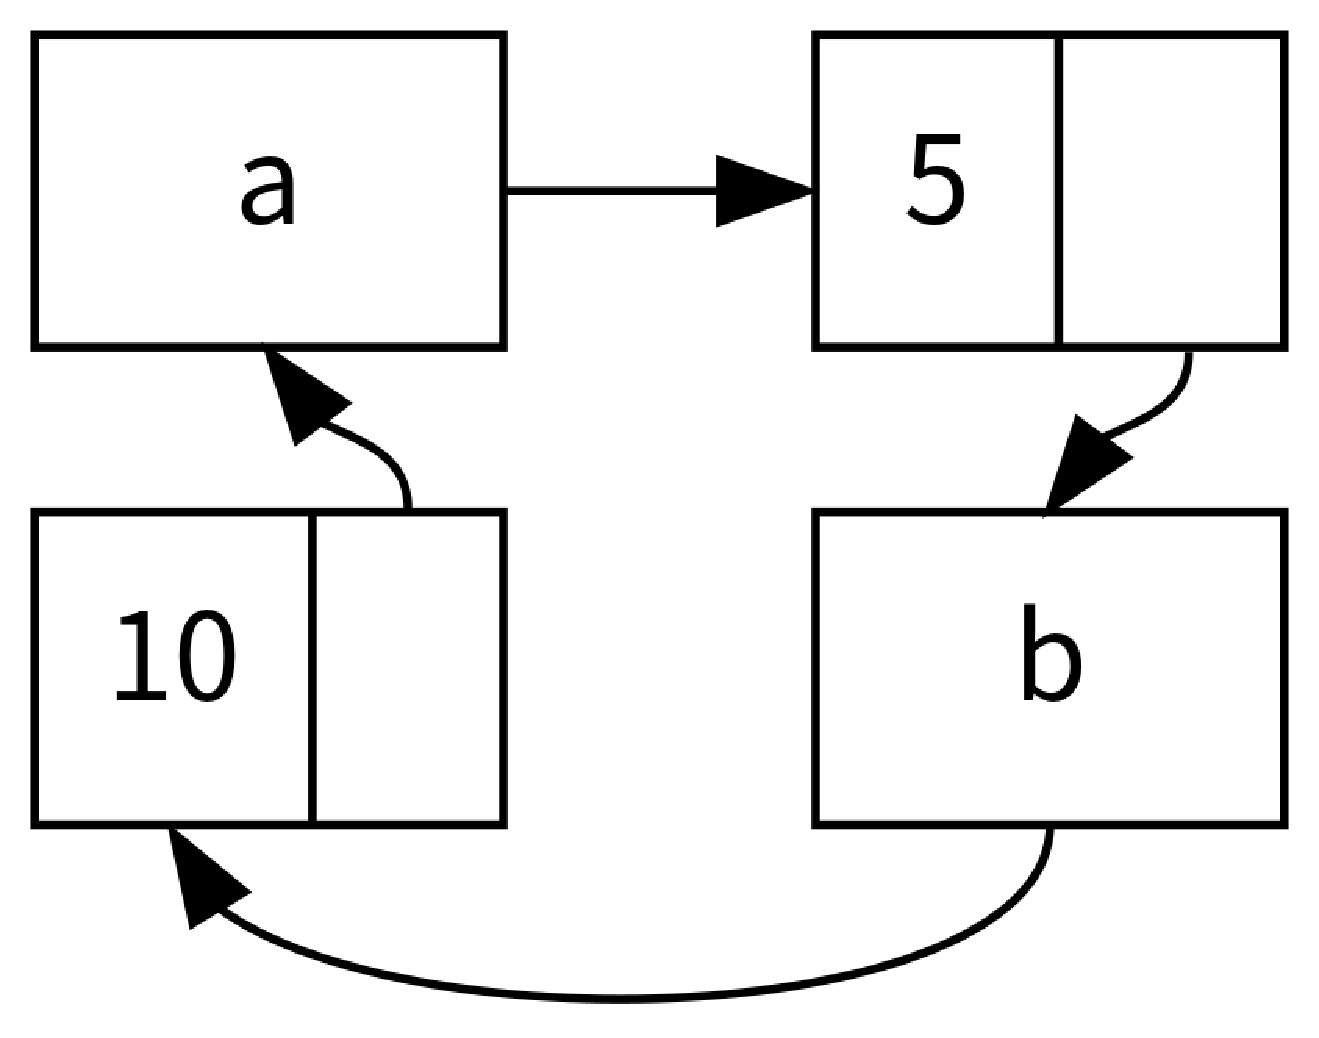
\includegraphics{img/trpl15-04.pdf}

{Figure 15-4: A reference cycle of lists \mintinline[]{text}{a} and
\mintinline[]{text}{b} pointing to each other}

If you uncomment the last \mintinline[]{text}{println!} and run the
program, Rust will try to print this cycle with \mintinline[]{text}{a}
pointing to \mintinline[]{text}{b} pointing to \mintinline[]{text}{a}
and so forth until it overflows the stack.

In this case, right after we create the reference cycle, the program
ends. The consequences of this cycle aren't very dire. However, if a
more complex program allocated lots of memory in a cycle and held onto
it for a long time, the program would use more memory than it needed and
might overwhelm the system, causing it to run out of available memory.

Creating reference cycles is not easily done, but it's not impossible
either. If you have \mintinline[]{text}{RefCell<T>} values that contain
\mintinline[]{text}{Rc<T>} values or similar nested combinations of
types with interior mutability and reference counting, you must ensure
that you don't create cycles; you can't rely on Rust to catch them.
Creating a reference cycle would be a logic bug in your program that you
should use automated tests, code reviews, and other software development
practices to minimize.

Another solution for avoiding reference cycles is reorganizing your data
structures so that some references express ownership and some references
don't. As a result, you can have cycles made up of some ownership
relationships and some non-ownership relationships, and only the
ownership relationships affect whether or not a value can be dropped. In
Listing 15-25, we always want \mintinline[]{text}{Cons} variants to own
their list, so reorganizing the data structure isn't possible. Let's
look at an example using graphs made up of parent nodes and child nodes
to see when non-ownership relationships are an appropriate way to
prevent reference cycles.

\hypertarget{preventing-reference-cycles-turning-an-rct-into-a-weakt}{%
\subsubsection{\texorpdfstring{Preventing Reference Cycles: Turning an
\mintinline[]{text}{Rc<T>} into a
\mintinline[]{text}{Weak<T>}}{Preventing Reference Cycles: Turning an  into a }}\label{preventing-reference-cycles-turning-an-rct-into-a-weakt}}

So far, we've demonstrated that calling \mintinline[]{text}{Rc::clone}
increases the \mintinline[]{text}{strong_count} of an
\mintinline[]{text}{Rc<T>} instance, and an \mintinline[]{text}{Rc<T>}
instance is only cleaned up if its \mintinline[]{text}{strong_count} is
0. You can also create a \emph{weak reference} to the value within an
\mintinline[]{text}{Rc<T>} instance by calling
\mintinline[]{text}{Rc::downgrade} and passing a reference to the
\mintinline[]{text}{Rc<T>}. When you call
\mintinline[]{text}{Rc::downgrade}, you get a smart pointer of type
\mintinline[]{text}{Weak<T>}. Instead of increasing the
\mintinline[]{text}{strong_count} in the \mintinline[]{text}{Rc<T>}
instance by 1, calling \mintinline[]{text}{Rc::downgrade} increases the
\mintinline[]{text}{weak_count} by 1. The \mintinline[]{text}{Rc<T>}
type uses \mintinline[]{text}{weak_count} to keep track of how many
\mintinline[]{text}{Weak<T>} references exist, similar to
\mintinline[]{text}{strong_count}. The difference is the
\mintinline[]{text}{weak_count} doesn't need to be 0 for the
\mintinline[]{text}{Rc<T>} instance to be cleaned up.

Strong references are how you can share ownership of an
\mintinline[]{text}{Rc<T>} instance. Weak references don't express an
ownership relationship. They won't cause a reference cycle because any
cycle involving some weak references will be broken once the strong
reference count of values involved is 0.

Because the value that \mintinline[]{text}{Weak<T>} references might
have been dropped, to do anything with the value that a
\mintinline[]{text}{Weak<T>} is pointing to, you must make sure the
value still exists. Do this by calling the \mintinline[]{text}{upgrade}
method on a \mintinline[]{text}{Weak<T>} instance, which will return an
\mintinline[]{text}{Option<Rc<T>>}. You'll get a result of
\mintinline[]{text}{Some} if the \mintinline[]{text}{Rc<T>} value has
not been dropped yet and a result of \mintinline[]{text}{None} if the
\mintinline[]{text}{Rc<T>} value has been dropped. Because
\mintinline[]{text}{upgrade} returns an \mintinline[]{text}{Option<T>},
Rust will ensure that the \mintinline[]{text}{Some} case and the
\mintinline[]{text}{None} case are handled, and there won't be an
invalid pointer.

As an example, rather than using a list whose items know only about the
next item, we'll create a tree whose items know about their children
items \emph{and} their parent items.

\hypertarget{creating-a-tree-data-structure-a-node-with-child-nodes}{%
\paragraph{\texorpdfstring{Creating a Tree Data Structure: a
\mintinline[]{text}{Node} with Child
Nodes}{Creating a Tree Data Structure: a  with Child Nodes}}\label{creating-a-tree-data-structure-a-node-with-child-nodes}}

To start, we'll build a tree with nodes that know about their child
nodes. We'll create a struct named \mintinline[]{text}{Node} that holds
its own \mintinline[]{text}{i32} value as well as references to its
children \mintinline[]{text}{Node} values:

{Filename: src/main.rs}

\begin{minted}[]{rust}
use std::rc::Rc;
use std::cell::RefCell;

#[derive(Debug)]
struct Node {
    value: i32,
    children: RefCell<Vec<Rc<Node>>>,
}
\end{minted}

We want a \mintinline[]{text}{Node} to own its children, and we want to
share that ownership with variables so we can access each
\mintinline[]{text}{Node} in the tree directly. To do this, we define
the \mintinline[]{text}{Vec<T>} items to be values of type
\mintinline[]{text}{Rc<Node>}. We also want to modify which nodes are
children of another node, so we have a \mintinline[]{text}{RefCell<T>}
in \mintinline[]{text}{children} around the
\mintinline[]{text}{Vec<Rc<Node>>}.

Next, we'll use our struct definition and create one
\mintinline[]{text}{Node} instance named \mintinline[]{text}{leaf} with
the value 3 and no children, and another instance named
\mintinline[]{text}{branch} with the value 5 and
\mintinline[]{text}{leaf} as one of its children, as shown in Listing
15-27:

{Filename: src/main.rs}

\begin{minted}[]{rust}
# use std::rc::Rc;
# use std::cell::RefCell;
#
# #[derive(Debug)]
# struct Node {
#     value: i32,
#    children: RefCell<Vec<Rc<Node>>>,
# }
#
fn main() {
    let leaf = Rc::new(Node {
        value: 3,
        children: RefCell::new(vec![]),
    });

    let branch = Rc::new(Node {
        value: 5,
        children: RefCell::new(vec![Rc::clone(&leaf)]),
    });
}
\end{minted}

{Listing 15-27: Creating a \mintinline[]{text}{leaf} node with no
children and a \mintinline[]{text}{branch} node with
\mintinline[]{text}{leaf} as one of its children}

We clone the \mintinline[]{text}{Rc<Node>} in \mintinline[]{text}{leaf}
and store that in \mintinline[]{text}{branch}, meaning the
\mintinline[]{text}{Node} in \mintinline[]{text}{leaf} now has two
owners: \mintinline[]{text}{leaf} and \mintinline[]{text}{branch}. We
can get from \mintinline[]{text}{branch} to \mintinline[]{text}{leaf}
through \mintinline[]{text}{branch.children}, but there's no way to get
from \mintinline[]{text}{leaf} to \mintinline[]{text}{branch}. The
reason is that \mintinline[]{text}{leaf} has no reference to
\mintinline[]{text}{branch} and doesn't know they're related. We want
\mintinline[]{text}{leaf} to know that \mintinline[]{text}{branch} is
its parent. We'll do that next.

\hypertarget{adding-a-reference-from-a-child-to-its-parent}{%
\paragraph{Adding a Reference from a Child to Its
Parent}\label{adding-a-reference-from-a-child-to-its-parent}}

To make the child node aware of its parent, we need to add a
\mintinline[]{text}{parent} field to our \mintinline[]{text}{Node}
struct definition. The trouble is in deciding what the type of
\mintinline[]{text}{parent} should be. We know it can't contain an
\mintinline[]{text}{Rc<T>}, because that would create a reference cycle
with \mintinline[]{text}{leaf.parent} pointing to
\mintinline[]{text}{branch} and \mintinline[]{text}{branch.children}
pointing to \mintinline[]{text}{leaf}, which would cause their
\mintinline[]{text}{strong_count} values to never be 0.

Thinking about the relationships another way, a parent node should own
its children: if a parent node is dropped, its child nodes should be
dropped as well. However, a child should not own its parent: if we drop
a child node, the parent should still exist. This is a case for weak
references!

So instead of \mintinline[]{text}{Rc<T>}, we'll make the type of
\mintinline[]{text}{parent} use \mintinline[]{text}{Weak<T>},
specifically a \mintinline[]{text}{RefCell<Weak<Node>>}. Now our
\mintinline[]{text}{Node} struct definition looks like this:

{Filename: src/main.rs}

\begin{minted}[]{rust}
use std::rc::{Rc, Weak};
use std::cell::RefCell;

#[derive(Debug)]
struct Node {
    value: i32,
    parent: RefCell<Weak<Node>>,
    children: RefCell<Vec<Rc<Node>>>,
}
\end{minted}

A node will be able to refer to its parent node but doesn't own its
parent. In Listing 15-28, we update \mintinline[]{text}{main} to use
this new definition so the \mintinline[]{text}{leaf} node will have a
way to refer to its parent, \mintinline[]{text}{branch}:

{Filename: src/main.rs}

\begin{minted}[]{rust}
# use std::rc::{Rc, Weak};
# use std::cell::RefCell;
#
# #[derive(Debug)]
# struct Node {
#     value: i32,
#     parent: RefCell<Weak<Node>>,
#     children: RefCell<Vec<Rc<Node>>>,
# }
#
fn main() {
    let leaf = Rc::new(Node {
        value: 3,
        parent: RefCell::new(Weak::new()),
        children: RefCell::new(vec![]),
    });

    println!("leaf parent = {:?}", leaf.parent.borrow().upgrade());

    let branch = Rc::new(Node {
        value: 5,
        parent: RefCell::new(Weak::new()),
        children: RefCell::new(vec![Rc::clone(&leaf)]),
    });

    *leaf.parent.borrow_mut() = Rc::downgrade(&branch);

    println!("leaf parent = {:?}", leaf.parent.borrow().upgrade());
}
\end{minted}

{Listing 15-28: A \mintinline[]{text}{leaf} node with a weak reference
to its parent node \mintinline[]{text}{branch}}

Creating the \mintinline[]{text}{leaf} node looks similar to how
creating the \mintinline[]{text}{leaf} node looked in Listing 15-27 with
the exception of the \mintinline[]{text}{parent} field:
\mintinline[]{text}{leaf} starts out without a parent, so we create a
new, empty \mintinline[]{text}{Weak<Node>} reference instance.

At this point, when we try to get a reference to the parent of
\mintinline[]{text}{leaf} by using the \mintinline[]{text}{upgrade}
method, we get a \mintinline[]{text}{None} value. We see this in the
output from the first \mintinline[]{text}{println!} statement:

\begin{minted}[]{text}
leaf parent = None
\end{minted}

When we create the \mintinline[]{text}{branch} node, it will also have a
new \mintinline[]{text}{Weak<Node>} reference in the
\mintinline[]{text}{parent} field, because \mintinline[]{text}{branch}
doesn't have a parent node. We still have \mintinline[]{text}{leaf} as
one of the children of \mintinline[]{text}{branch}. Once we have the
\mintinline[]{text}{Node} instance in \mintinline[]{text}{branch}, we
can modify \mintinline[]{text}{leaf} to give it a
\mintinline[]{text}{Weak<Node>} reference to its parent. We use the
\mintinline[]{text}{borrow_mut} method on the
\mintinline[]{text}{RefCell<Weak<Node>>} in the
\mintinline[]{text}{parent} field of \mintinline[]{text}{leaf}, and then
we use the \mintinline[]{text}{Rc::downgrade} function to create a
\mintinline[]{text}{Weak<Node>} reference to \mintinline[]{text}{branch}
from the \mintinline[]{text}{Rc<Node>} in \mintinline[]{text}{branch.}

When we print the parent of \mintinline[]{text}{leaf} again, this time
we'll get a \mintinline[]{text}{Some} variant holding
\mintinline[]{text}{branch}: now \mintinline[]{text}{leaf} can access
its parent! When we print \mintinline[]{text}{leaf}, we also avoid the
cycle that eventually ended in a stack overflow like we had in Listing
15-26; the \mintinline[]{text}{Weak<Node>} references are printed as
\mintinline[]{text}{(Weak)}:

\begin{minted}[]{text}
leaf parent = Some(Node { value: 5, parent: RefCell { value: (Weak) },
children: RefCell { value: [Node { value: 3, parent: RefCell { value: (Weak) },
children: RefCell { value: [] } }] } })
\end{minted}

The lack of infinite output indicates that this code didn't create a
reference cycle. We can also tell this by looking at the values we get
from calling \mintinline[]{text}{Rc::strong_count} and
\mintinline[]{text}{Rc::weak_count}.

\hypertarget{visualizing-changes-to-strong_count-and-weak_count}{%
\paragraph{\texorpdfstring{Visualizing Changes to
\mintinline[]{text}{strong_count} and
\mintinline[]{text}{weak_count}}{Visualizing Changes to  and }}\label{visualizing-changes-to-strong_count-and-weak_count}}

Let's look at how the \mintinline[]{text}{strong_count} and
\mintinline[]{text}{weak_count} values of the
\mintinline[]{text}{Rc<Node>} instances change by creating a new inner
scope and moving the creation of \mintinline[]{text}{branch} into that
scope. By doing so, we can see what happens when
\mintinline[]{text}{branch} is created and then dropped when it goes out
of scope. The modifications are shown in Listing 15-29:

{Filename: src/main.rs}

\begin{minted}[]{rust}
# use std::rc::{Rc, Weak};
# use std::cell::RefCell;
#
# #[derive(Debug)]
# struct Node {
#     value: i32,
#     parent: RefCell<Weak<Node>>,
#     children: RefCell<Vec<Rc<Node>>>,
# }
#
fn main() {
    let leaf = Rc::new(Node {
        value: 3,
        parent: RefCell::new(Weak::new()),
        children: RefCell::new(vec![]),
    });

    println!(
        "leaf strong = {}, weak = {}",
        Rc::strong_count(&leaf),
        Rc::weak_count(&leaf),
    );

    {
        let branch = Rc::new(Node {
            value: 5,
            parent: RefCell::new(Weak::new()),
            children: RefCell::new(vec![Rc::clone(&leaf)]),
        });

        *leaf.parent.borrow_mut() = Rc::downgrade(&branch);

        println!(
            "branch strong = {}, weak = {}",
            Rc::strong_count(&branch),
            Rc::weak_count(&branch),
        );

        println!(
            "leaf strong = {}, weak = {}",
            Rc::strong_count(&leaf),
            Rc::weak_count(&leaf),
        );
    }

    println!("leaf parent = {:?}", leaf.parent.borrow().upgrade());
    println!(
        "leaf strong = {}, weak = {}",
        Rc::strong_count(&leaf),
        Rc::weak_count(&leaf),
    );
}
\end{minted}

{Listing 15-29: Creating \mintinline[]{text}{branch} in an inner scope
and examining strong and weak reference counts}

After \mintinline[]{text}{leaf} is created, its
\mintinline[]{text}{Rc<Node>} has a strong count of 1 and a weak count
of 0. In the inner scope, we create \mintinline[]{text}{branch} and
associate it with \mintinline[]{text}{leaf}, at which point when we
print the counts, the \mintinline[]{text}{Rc<Node>} in
\mintinline[]{text}{branch} will have a strong count of 1 and a weak
count of 1 (for \mintinline[]{text}{leaf.parent} pointing to
\mintinline[]{text}{branch} with a \mintinline[]{text}{Weak<Node>}).
When we print the counts in \mintinline[]{text}{leaf}, we'll see it will
have a strong count of 2, because \mintinline[]{text}{branch} now has a
clone of the \mintinline[]{text}{Rc<Node>} of \mintinline[]{text}{leaf}
stored in \mintinline[]{text}{branch.children}, but will still have a
weak count of 0.

When the inner scope ends, \mintinline[]{text}{branch} goes out of scope
and the strong count of the \mintinline[]{text}{Rc<Node>} decreases to
0, so its \mintinline[]{text}{Node} is dropped. The weak count of 1 from
\mintinline[]{text}{leaf.parent} has no bearing on whether or not
\mintinline[]{text}{Node} is dropped, so we don't get any memory leaks!

If we try to access the parent of \mintinline[]{text}{leaf} after the
end of the scope, we'll get \mintinline[]{text}{None} again. At the end
of the program, the \mintinline[]{text}{Rc<Node>} in
\mintinline[]{text}{leaf} has a strong count of 1 and a weak count of 0,
because the variable \mintinline[]{text}{leaf} is now the only reference
to the \mintinline[]{text}{Rc<Node>} again.

All of the logic that manages the counts and value dropping is built
into \mintinline[]{text}{Rc<T>} and \mintinline[]{text}{Weak<T>} and
their implementations of the \mintinline[]{text}{Drop} trait. By
specifying that the relationship from a child to its parent should be a
\mintinline[]{text}{Weak<T>} reference in the definition of
\mintinline[]{text}{Node}, you're able to have parent nodes point to
child nodes and vice versa without creating a reference cycle and memory
leaks.

\hypertarget{summary-14}{%
\subsection{Summary}\label{summary-14}}

This chapter covered how to use smart pointers to make different
guarantees and trade-offs from those Rust makes by default with regular
references. The \mintinline[]{text}{Box<T>} type has a known size and
points to data allocated on the heap. The \mintinline[]{text}{Rc<T>}
type keeps track of the number of references to data on the heap so that
data can have multiple owners. The \mintinline[]{text}{RefCell<T>} type
with its interior mutability gives us a type that we can use when we
need an immutable type but need to change an inner value of that type;
it also enforces the borrowing rules at runtime instead of at compile
time.

Also discussed were the \mintinline[]{text}{Deref} and
\mintinline[]{text}{Drop} traits, which enable a lot of the
functionality of smart pointers. We explored reference cycles that can
cause memory leaks and how to prevent them using
\mintinline[]{text}{Weak<T>}.

If this chapter has piqued your interest and you want to implement your
own smart pointers, check out
\href{https://doc.rust-lang.org/stable/nomicon/}{``The Rustonomicon''}
for more useful information.

Next, we'll talk about concurrency in Rust. You'll even learn about a
few new smart pointers.

\hypertarget{fearless-concurrency}{%
\section{Fearless Concurrency}\label{fearless-concurrency}}

Handling concurrent programming safely and efficiently is another of
Rust's major goals. \emph{Concurrent programming}, where different parts
of a program execute independently, and \emph{parallel programming},
where different parts of a program execute at the same time, are
becoming increasingly important as more computers take advantage of
their multiple processors. Historically, programming in these contexts
has been difficult and error prone: Rust hopes to change that.

Initially, the Rust team thought that ensuring memory safety and
preventing concurrency problems were two separate challenges to be
solved with different methods. Over time, the team discovered that the
ownership and type systems are a powerful set of tools to help manage
memory safety \emph{and} concurrency problems! By leveraging ownership
and type checking, many concurrency errors are compile-time errors in
Rust rather than runtime errors. Therefore, rather than making you spend
lots of time trying to reproduce the exact circumstances under which a
runtime concurrency bug occurs, incorrect code will refuse to compile
and present an error explaining the problem. As a result, you can fix
your code while you're working on it rather than potentially after it
has been shipped to production. We've nicknamed this aspect of Rust
\emph{fearless} \emph{concurrency}. Fearless concurrency allows you to
write code that is free of subtle bugs and is easy to refactor without
introducing new bugs.

\begin{quote}
Note: For simplicity's sake, we'll refer to many of the problems as
\emph{concurrent} rather than being more precise by saying
\emph{concurrent and/or parallel}. If this book were about concurrency
and/or parallelism, we'd be more specific. For this chapter, please
mentally substitute \emph{concurrent and/or parallel} whenever we use
\emph{concurrent}.
\end{quote}

Many languages are dogmatic about the solutions they offer for handling
concurrent problems. For example, Erlang has elegant functionality for
message-passing concurrency but has only obscure ways to share state
between threads. Supporting only a subset of possible solutions is a
reasonable strategy for higher-level languages, because a higher-level
language promises benefits from giving up some control to gain
abstractions. However, lower-level languages are expected to provide the
solution with the best performance in any given situation and have fewer
abstractions over the hardware. Therefore, Rust offers a variety of
tools for modeling problems in whatever way is appropriate for your
situation and requirements.

Here are the topics we'll cover in this chapter:

\begin{itemize}
\tightlist
\item
  How to create threads to run multiple pieces of code at the same time
\item
  \emph{Message-passing} concurrency, where channels send messages
  between threads
\item
  \emph{Shared-state} concurrency, where multiple threads have access to
  some piece of data
\item
  The \mintinline[]{text}{Sync} and \mintinline[]{text}{Send} traits,
  which extend Rust's concurrency guarantees to user-defined types as
  well as types provided by the standard library
\end{itemize}

\hypertarget{using-threads-to-run-code-simultaneously}{%
\subsection{Using Threads to Run Code
Simultaneously}\label{using-threads-to-run-code-simultaneously}}

In most current operating systems, an executed program's code is run in
a \emph{process}, and the operating system manages multiple processes at
once. Within your program, you can also have independent parts that run
simultaneously. The features that run these independent parts are called
\emph{threads}.

Splitting the computation in your program into multiple threads can
improve performance because the program does multiple tasks at the same
time, but it also adds complexity. Because threads can run
simultaneously, there's no inherent guarantee about the order in which
parts of your code on different threads will run. This can lead to
problems, such as:

\begin{itemize}
\tightlist
\item
  Race conditions, where threads are accessing data or resources in an
  inconsistent order
\item
  Deadlocks, where two threads are waiting for each other to finish
  using a resource the other thread has, preventing both threads from
  continuing
\item
  Bugs that happen only in certain situations and are hard to reproduce
  and fix reliably
\end{itemize}

Rust attempts to mitigate the negative effects of using threads, but
programming in a multithreaded context still takes careful thought and
requires a code structure that is different from that in programs
running in a single thread.

Programming languages implement threads in a few different ways. Many
operating systems provide an API for creating new threads. This model
where a language calls the operating system APIs to create threads is
sometimes called \emph{1:1}, meaning one operating system thread per one
language thread.

Many programming languages provide their own special implementation of
threads. Programming language-provided threads are known as \emph{green}
threads, and languages that use these green threads will execute them in
the context of a different number of operating system threads. For this
reason, the green-threaded model is called the \emph{M:N} model: there
are \mintinline[]{text}{M} green threads per \mintinline[]{text}{N}
operating system threads, where \mintinline[]{text}{M} and
\mintinline[]{text}{N} are not necessarily the same number.

Each model has its own advantages and trade-offs, and the trade-off most
important to Rust is runtime support. \emph{Runtime} is a confusing term
and can have different meanings in different contexts.

In this context, by \emph{runtime} we mean code that is included by the
language in every binary. This code can be large or small depending on
the language, but every non-assembly language will have some amount of
runtime code. For that reason, colloquially when people say a language
has ``no runtime,'' they often mean ``small runtime.'' Smaller runtimes
have fewer features but have the advantage of resulting in smaller
binaries, which make it easier to combine the language with other
languages in more contexts. Although many languages are okay with
increasing the runtime size in exchange for more features, Rust needs to
have nearly no runtime and cannot compromise on being able to call into
C to maintain performance.

The green-threading M:N model requires a larger language runtime to
manage threads. As such, the Rust standard library only provides an
implementation of 1:1 threading. Because Rust is such a low-level
language, there are crates that implement M:N threading if you would
rather trade overhead for aspects such as more control over which
threads run when and lower costs of context switching, for example.

Now that we've defined threads in Rust, let's explore how to use the
thread-related API provided by the standard library.

\hypertarget{creating-a-new-thread-with-spawn}{%
\subsubsection{\texorpdfstring{Creating a New Thread with
\mintinline[]{text}{spawn}}{Creating a New Thread with }}\label{creating-a-new-thread-with-spawn}}

To create a new thread, we call the \mintinline[]{text}{thread::spawn}
function and pass it a closure (we talked about closures in Chapter 13)
containing the code we want to run in the new thread. The example in
Listing 16-1 prints some text from a main thread and other text from a
new thread:

{Filename: src/main.rs}

\begin{minted}[]{rust}
use std::thread;
use std::time::Duration;

fn main() {
    thread::spawn(|| {
        for i in 1..10 {
            println!("hi number {} from the spawned thread!", i);
            thread::sleep(Duration::from_millis(1));
        }
    });

    for i in 1..5 {
        println!("hi number {} from the main thread!", i);
        thread::sleep(Duration::from_millis(1));
    }
}
\end{minted}

{Listing 16-1: Creating a new thread to print one thing while the main
thread prints something else}

Note that with this function, the new thread will be stopped when the
main thread ends, whether or not it has finished running. The output
from this program might be a little different every time, but it will
look similar to the following:

\begin{minted}[]{text}
hi number 1 from the main thread!
hi number 1 from the spawned thread!
hi number 2 from the main thread!
hi number 2 from the spawned thread!
hi number 3 from the main thread!
hi number 3 from the spawned thread!
hi number 4 from the main thread!
hi number 4 from the spawned thread!
hi number 5 from the spawned thread!
\end{minted}

The calls to \mintinline[]{text}{thread::sleep} force a thread to stop
its execution for a short duration, allowing a different thread to run.
The threads will probably take turns, but that isn't guaranteed: it
depends on how your operating system schedules the threads. In this run,
the main thread printed first, even though the print statement from the
spawned thread appears first in the code. And even though we told the
spawned thread to print until \mintinline[]{text}{i} is 9, it only got
to 5 before the main thread shut down.

If you run this code and only see output from the main thread, or don't
see any overlap, try increasing the numbers in the ranges to create more
opportunities for the operating system to switch between the threads.

\hypertarget{waiting-for-all-threads-to-finish-using-join-handles}{%
\subsubsection{\texorpdfstring{Waiting for All Threads to Finish Using
\mintinline[]{text}{join}
Handles}{Waiting for All Threads to Finish Using  Handles}}\label{waiting-for-all-threads-to-finish-using-join-handles}}

The code in Listing 16-1 not only stops the spawned thread prematurely
most of the time due to the main thread ending, but also can't guarantee
that the spawned thread will get to run at all. The reason is that there
is no guarantee on the order in which threads run!

We can fix the problem of the spawned thread not getting to run, or not
getting to run completely, by saving the return value of
\mintinline[]{text}{thread::spawn} in a variable. The return type of
\mintinline[]{text}{thread::spawn} is \mintinline[]{text}{JoinHandle}. A
\mintinline[]{text}{JoinHandle} is an owned value that, when we call the
\mintinline[]{text}{join} method on it, will wait for its thread to
finish. Listing 16-2 shows how to use the
\mintinline[]{text}{JoinHandle} of the thread we created in Listing 16-1
and call \mintinline[]{text}{join} to make sure the spawned thread
finishes before \mintinline[]{text}{main} exits:

{Filename: src/main.rs}

\begin{minted}[]{rust}
use std::thread;
use std::time::Duration;

fn main() {
    let handle = thread::spawn(|| {
        for i in 1..10 {
            println!("hi number {} from the spawned thread!", i);
            thread::sleep(Duration::from_millis(1));
        }
    });

    for i in 1..5 {
        println!("hi number {} from the main thread!", i);
        thread::sleep(Duration::from_millis(1));
    }

    handle.join().unwrap();
}
\end{minted}

{Listing 16-2: Saving a \mintinline[]{text}{JoinHandle} from
\mintinline[]{text}{thread::spawn} to guarantee the thread is run to
completion}

Calling \mintinline[]{text}{join} on the handle blocks the thread
currently running until the thread represented by the handle terminates.
\emph{Blocking} a thread means that thread is prevented from performing
work or exiting. Because we've put the call to \mintinline[]{text}{join}
after the main thread's \mintinline[]{text}{for} loop, running Listing
16-2 should produce output similar to this:

\begin{minted}[]{text}
hi number 1 from the main thread!
hi number 2 from the main thread!
hi number 1 from the spawned thread!
hi number 3 from the main thread!
hi number 2 from the spawned thread!
hi number 4 from the main thread!
hi number 3 from the spawned thread!
hi number 4 from the spawned thread!
hi number 5 from the spawned thread!
hi number 6 from the spawned thread!
hi number 7 from the spawned thread!
hi number 8 from the spawned thread!
hi number 9 from the spawned thread!
\end{minted}

The two threads continue alternating, but the main thread waits because
of the call to \mintinline[]{text}{handle.join()} and does not end until
the spawned thread is finished.

But let's see what happens when we instead move
\mintinline[]{text}{handle.join()} before the \mintinline[]{text}{for}
loop in \mintinline[]{text}{main}, like this:

{Filename: src/main.rs}

\begin{minted}[]{rust}
use std::thread;
use std::time::Duration;

fn main() {
    let handle = thread::spawn(|| {
        for i in 1..10 {
            println!("hi number {} from the spawned thread!", i);
            thread::sleep(Duration::from_millis(1));
        }
    });

    handle.join().unwrap();

    for i in 1..5 {
        println!("hi number {} from the main thread!", i);
        thread::sleep(Duration::from_millis(1));
    }
}
\end{minted}

The main thread will wait for the spawned thread to finish and then run
its \mintinline[]{text}{for} loop, so the output won't be interleaved
anymore, as shown here:

\begin{minted}[]{text}
hi number 1 from the spawned thread!
hi number 2 from the spawned thread!
hi number 3 from the spawned thread!
hi number 4 from the spawned thread!
hi number 5 from the spawned thread!
hi number 6 from the spawned thread!
hi number 7 from the spawned thread!
hi number 8 from the spawned thread!
hi number 9 from the spawned thread!
hi number 1 from the main thread!
hi number 2 from the main thread!
hi number 3 from the main thread!
hi number 4 from the main thread!
\end{minted}

Small details, such as where \mintinline[]{text}{join} is called, can
affect whether or not your threads run at the same time.

\hypertarget{using-move-closures-with-threads}{%
\subsubsection{\texorpdfstring{Using \mintinline[]{text}{move} Closures
with
Threads}{Using  Closures with Threads}}\label{using-move-closures-with-threads}}

The \mintinline[]{text}{move} closure is often used alongside
\mintinline[]{text}{thread::spawn} because it allows you to use data
from one thread in another thread.

In Chapter 13, we mentioned we can use the \mintinline[]{text}{move}
keyword before the parameter list of a closure to force the closure to
take ownership of the values it uses in the environment. This technique
is especially useful when creating new threads in order to transfer
ownership of values from one thread to another.

Notice in Listing 16-1 that the closure we pass to
\mintinline[]{text}{thread::spawn} takes no arguments: we're not using
any data from the main thread in the spawned thread's code. To use data
from the main thread in the spawned thread, the spawned thread's closure
must capture the values it needs. Listing 16-3 shows an attempt to
create a vector in the main thread and use it in the spawned thread.
However, this won't yet work, as you'll see in a moment.

{Filename: src/main.rs}

\begin{minted}[]{rust}
use std::thread;

fn main() {
    let v = vec![1, 2, 3];

    let handle = thread::spawn(|| {
        println!("Here's a vector: {:?}", v);
    });

    handle.join().unwrap();
}
\end{minted}

{Listing 16-3: Attempting to use a vector created by the main thread in
another thread}

The closure uses \mintinline[]{text}{v}, so it will capture
\mintinline[]{text}{v} and make it part of the closure's environment.
Because \mintinline[]{text}{thread::spawn} runs this closure in a new
thread, we should be able to access \mintinline[]{text}{v} inside that
new thread. But when we compile this example, we get the following
error:

\begin{minted}[]{text}
error[E0373]: closure may outlive the current function, but it borrows `v`,
which is owned by the current function
 --> src/main.rs:6:32
  |
6 |     let handle = thread::spawn(|| {
  |                                ^^ may outlive borrowed value `v`
7 |         println!("Here's a vector: {:?}", v);
  |                                           - `v` is borrowed here
  |
help: to force the closure to take ownership of `v` (and any other referenced
variables), use the `move` keyword
  |
6 |     let handle = thread::spawn(move || {
  |                                ^^^^^^^
\end{minted}

Rust \emph{infers} how to capture \mintinline[]{text}{v}, and because
\mintinline[]{text}{println!} only needs a reference to
\mintinline[]{text}{v}, the closure tries to borrow
\mintinline[]{text}{v}. However, there's a problem: Rust can't tell how
long the spawned thread will run, so it doesn't know if the reference to
\mintinline[]{text}{v} will always be valid.

Listing 16-4 provides a scenario that's more likely to have a reference
to \mintinline[]{text}{v} that won't be valid:

{Filename: src/main.rs}

\begin{minted}[]{rust}
use std::thread;

fn main() {
    let v = vec![1, 2, 3];

    let handle = thread::spawn(|| {
        println!("Here's a vector: {:?}", v);
    });

    drop(v); // oh no!

    handle.join().unwrap();
}
\end{minted}

{Listing 16-4: A thread with a closure that attempts to capture a
reference to \mintinline[]{text}{v} from a main thread that drops
\mintinline[]{text}{v}}

If we were allowed to run this code, there's a possibility the spawned
thread would be immediately put in the background without running at
all. The spawned thread has a reference to \mintinline[]{text}{v}
inside, but the main thread immediately drops \mintinline[]{text}{v},
using the \mintinline[]{text}{drop} function we discussed in Chapter 15.
Then, when the spawned thread starts to execute, \mintinline[]{text}{v}
is no longer valid, so a reference to it is also invalid. Oh no!

To fix the compiler error in Listing 16-3, we can use the error
message's advice:

\begin{minted}[]{text}
help: to force the closure to take ownership of `v` (and any other referenced
variables), use the `move` keyword
  |
6 |     let handle = thread::spawn(move || {
  |                                ^^^^^^^
\end{minted}

By adding the \mintinline[]{text}{move} keyword before the closure, we
force the closure to take ownership of the values it's using rather than
allowing Rust to infer that it should borrow the values. The
modification to Listing 16-3 shown in Listing 16-5 will compile and run
as we intend:

{Filename: src/main.rs}

\begin{minted}[]{rust}
use std::thread;

fn main() {
    let v = vec![1, 2, 3];

    let handle = thread::spawn(move || {
        println!("Here's a vector: {:?}", v);
    });

    handle.join().unwrap();
}
\end{minted}

{Listing 16-5: Using the \mintinline[]{text}{move} keyword to force a
closure to take ownership of the values it uses}

What would happen to the code in Listing 16-4 where the main thread
called \mintinline[]{text}{drop} if we use a \mintinline[]{text}{move}
closure? Would \mintinline[]{text}{move} fix that case? Unfortunately,
no; we would get a different error because what Listing 16-4 is trying
to do isn't allowed for a different reason. If we added
\mintinline[]{text}{move} to the closure, we would move
\mintinline[]{text}{v} into the closure's environment, and we could no
longer call \mintinline[]{text}{drop} on it in the main thread. We would
get this compiler error instead:

\begin{minted}[]{text}
error[E0382]: use of moved value: `v`
  --> src/main.rs:10:10
   |
6  |     let handle = thread::spawn(move || {
   |                                ------- value moved (into closure) here
...
10 |     drop(v); // oh no!
   |          ^ value used here after move
   |
   = note: move occurs because `v` has type `std::vec::Vec<i32>`, which does
   not implement the `Copy` trait
\end{minted}

Rust's ownership rules have saved us again! We got an error from the
code in Listing 16-3 because Rust was being conservative and only
borrowing \mintinline[]{text}{v} for the thread, which meant the main
thread could theoretically invalidate the spawned thread's reference. By
telling Rust to move ownership of \mintinline[]{text}{v} to the spawned
thread, we're guaranteeing Rust that the main thread won't use
\mintinline[]{text}{v} anymore. If we change Listing 16-4 in the same
way, we're then violating the ownership rules when we try to use
\mintinline[]{text}{v} in the main thread. The \mintinline[]{text}{move}
keyword overrides Rust's conservative default of borrowing; it doesn't
let us violate the ownership rules.

With a basic understanding of threads and the thread API, let's look at
what we can \emph{do} with threads.

\hypertarget{using-message-passing-to-transfer-data-between-threads}{%
\subsection{Using Message Passing to Transfer Data Between
Threads}\label{using-message-passing-to-transfer-data-between-threads}}

One increasingly popular approach to ensuring safe concurrency is
\emph{message passing}, where threads or actors communicate by sending
each other messages containing data. Here's the idea in a slogan from
\href{http://golang.org/doc/effective_go.html}{the Go language
documentation}: ``Do not communicate by sharing memory; instead, share
memory by communicating.''

One major tool Rust has for accomplishing message-sending concurrency is
the \emph{channel}, a programming concept that Rust's standard library
provides an implementation of. You can imagine a channel in programming
as being like a channel of water, such as a stream or a river. If you
put something like a rubber duck or boat into a stream, it will travel
downstream to the end of the waterway.

A channel in programming has two halves: a transmitter and a receiver.
The transmitter half is the upstream location where you put rubber ducks
into the river, and the receiver half is where the rubber duck ends up
downstream. One part of your code calls methods on the transmitter with
the data you want to send, and another part checks the receiving end for
arriving messages. A channel is said to be \emph{closed} if either the
transmitter or receiver half is dropped.

Here, we'll work up to a program that has one thread to generate values
and send them down a channel, and another thread that will receive the
values and print them out. We'll be sending simple values between
threads using a channel to illustrate the feature. Once you're familiar
with the technique, you could use channels to implement a chat system or
a system where many threads perform parts of a calculation and send the
parts to one thread that aggregates the results.

First, in Listing 16-6, we'll create a channel but not do anything with
it. Note that this won't compile yet because Rust can't tell what type
of values we want to send over the channel.

{Filename: src/main.rs}

\begin{minted}[]{rust}
use std::sync::mpsc;

fn main() {
    let (tx, rx) = mpsc::channel();
}
\end{minted}

{Listing 16-6: Creating a channel and assigning the two halves to
\mintinline[]{text}{tx} and \mintinline[]{text}{rx}}

We create a new channel using the \mintinline[]{text}{mpsc::channel}
function; \mintinline[]{text}{mpsc} stands for \emph{multiple producer,
single consumer}. In short, the way Rust's standard library implements
channels means a channel can have multiple \emph{sending} ends that
produce values but only one \emph{receiving} end that consumes those
values. Imagine multiple streams flowing together into one big river:
everything sent down any of the streams will end up in one river at the
end. We'll start with a single producer for now, but we'll add multiple
producers when we get this example working.

The \mintinline[]{text}{mpsc::channel} function returns a tuple, the
first element of which is the sending end and the second element is the
receiving end. The abbreviations \mintinline[]{text}{tx} and
\mintinline[]{text}{rx} are traditionally used in many fields for
\emph{transmitter} and \emph{receiver} respectively, so we name our
variables as such to indicate each end. We're using a
\mintinline[]{text}{let} statement with a pattern that destructures the
tuples; we'll discuss the use of patterns in \mintinline[]{text}{let}
statements and destructuring in Chapter 18. Using a
\mintinline[]{text}{let} statement this way is a convenient approach to
extract the pieces of the tuple returned by
\mintinline[]{text}{mpsc::channel}.

Let's move the transmitting end into a spawned thread and have it send
one string so the spawned thread is communicating with the main thread,
as shown in Listing 16-7. This is like putting a rubber duck in the
river upstream or sending a chat message from one thread to another.

{Filename: src/main.rs}

\begin{minted}[]{rust}
use std::thread;
use std::sync::mpsc;

fn main() {
    let (tx, rx) = mpsc::channel();

    thread::spawn(move || {
        let val = String::from("hi");
        tx.send(val).unwrap();
    });
}
\end{minted}

{Listing 16-7: Moving \mintinline[]{text}{tx} to a spawned thread and
sending ``hi''}

Again, we're using \mintinline[]{text}{thread::spawn} to create a new
thread and then using \mintinline[]{text}{move} to move
\mintinline[]{text}{tx} into the closure so the spawned thread owns
\mintinline[]{text}{tx}. The spawned thread needs to own the
transmitting end of the channel to be able to send messages through the
channel.

The transmitting end has a \mintinline[]{text}{send} method that takes
the value we want to send. The \mintinline[]{text}{send} method returns
a \mintinline[]{text}{Result<T, E>} type, so if the receiving end has
already been dropped and there's nowhere to send a value, the send
operation will return an error. In this example, we're calling
\mintinline[]{text}{unwrap} to panic in case of an error. But in a real
application, we would handle it properly: return to Chapter 9 to review
strategies for proper error handling.

In Listing 16-8, we'll get the value from the receiving end of the
channel in the main thread. This is like retrieving the rubber duck from
the water at the end of the river or like getting a chat message.

{Filename: src/main.rs}

\begin{minted}[]{rust}
use std::thread;
use std::sync::mpsc;

fn main() {
    let (tx, rx) = mpsc::channel();

    thread::spawn(move || {
        let val = String::from("hi");
        tx.send(val).unwrap();
    });

    let received = rx.recv().unwrap();
    println!("Got: {}", received);
}
\end{minted}

{Listing 16-8: Receiving the value ``hi'' in the main thread and
printing it}

The receiving end of a channel has two useful methods:
\mintinline[]{text}{recv} and \mintinline[]{text}{try_recv}. We're using
\mintinline[]{text}{recv}, short for \emph{receive}, which will block
the main thread's execution and wait until a value is sent down the
channel. Once a value is sent, \mintinline[]{text}{recv} will return it
in a \mintinline[]{text}{Result<T, E>}. When the sending end of the
channel closes, \mintinline[]{text}{recv} will return an error to signal
that no more values will be coming.

The \mintinline[]{text}{try_recv} method doesn't block, but will instead
return a \mintinline[]{text}{Result<T, E>} immediately: an
\mintinline[]{text}{Ok} value holding a message if one is available and
an \mintinline[]{text}{Err} value if there aren't any messages this
time. Using \mintinline[]{text}{try_recv} is useful if this thread has
other work to do while waiting for messages: we could write a loop that
calls \mintinline[]{text}{try_recv} every so often, handles a message if
one is available, and otherwise does other work for a little while until
checking again.

We've used \mintinline[]{text}{recv} in this example for simplicity; we
don't have any other work for the main thread to do other than wait for
messages, so blocking the main thread is appropriate.

When we run the code in Listing 16-8, we'll see the value printed from
the main thread:

\begin{minted}[]{text}
Got: hi
\end{minted}

Perfect!

\hypertarget{channels-and-ownership-transference}{%
\subsubsection{Channels and Ownership
Transference}\label{channels-and-ownership-transference}}

The ownership rules play a vital role in message sending because they
help you write safe, concurrent code. Preventing errors in concurrent
programming is the advantage of thinking about ownership throughout your
Rust programs. Let's do an experiment to show how channels and ownership
work together to prevent problems: we'll try to use a
\mintinline[]{text}{val} value in the spawned thread \emph{after} we've
sent it down the channel. Try compiling the code in Listing 16-9 to see
why this code isn't allowed:

{Filename: src/main.rs}

\begin{minted}[]{rust}
use std::thread;
use std::sync::mpsc;

fn main() {
    let (tx, rx) = mpsc::channel();

    thread::spawn(move || {
        let val = String::from("hi");
        tx.send(val).unwrap();
        println!("val is {}", val);
    });

    let received = rx.recv().unwrap();
    println!("Got: {}", received);
}
\end{minted}

{Listing 16-9: Attempting to use \mintinline[]{text}{val} after we've
sent it down the channel}

Here, we try to print \mintinline[]{text}{val} after we've sent it down
the channel via \mintinline[]{text}{tx.send}. Allowing this would be a
bad idea: once the value has been sent to another thread, that thread
could modify or drop it before we try to use the value again.
Potentially, the other thread's modifications could cause errors or
unexpected results due to inconsistent or nonexistent data. However,
Rust gives us an error if we try to compile the code in Listing 16-9:

\begin{minted}[]{text}
error[E0382]: use of moved value: `val`
  --> src/main.rs:10:31
   |
9  |         tx.send(val).unwrap();
   |                 --- value moved here
10 |         println!("val is {}", val);
   |                               ^^^ value used here after move
   |
   = note: move occurs because `val` has type `std::string::String`, which does
not implement the `Copy` trait
\end{minted}

Our concurrency mistake has caused a compile time error. The
\mintinline[]{text}{send} function takes ownership of its parameter, and
when the value is moved, the receiver takes ownership of it. This stops
us from accidentally using the value again after sending it; the
ownership system checks that everything is okay.

\hypertarget{sending-multiple-values-and-seeing-the-receiver-waiting}{%
\subsubsection{Sending Multiple Values and Seeing the Receiver
Waiting}\label{sending-multiple-values-and-seeing-the-receiver-waiting}}

The code in Listing 16-8 compiled and ran, but it didn't clearly show us
that two separate threads were talking to each other over the channel.
In Listing 16-10 we've made some modifications that will prove the code
in Listing 16-8 is running concurrently: the spawned thread will now
send multiple messages and pause for a second between each message.

{Filename: src/main.rs}

\begin{minted}[]{rust}
use std::thread;
use std::sync::mpsc;
use std::time::Duration;

fn main() {
    let (tx, rx) = mpsc::channel();

    thread::spawn(move || {
        let vals = vec![
            String::from("hi"),
            String::from("from"),
            String::from("the"),
            String::from("thread"),
        ];

        for val in vals {
            tx.send(val).unwrap();
            thread::sleep(Duration::from_secs(1));
        }
    });

    for received in rx {
        println!("Got: {}", received);
    }
}
\end{minted}

{Listing 16-10: Sending multiple messages and pausing between each}

This time, the spawned thread has a vector of strings that we want to
send to the main thread. We iterate over them, sending each
individually, and pause between each by calling the
\mintinline[]{text}{thread::sleep} function with a
\mintinline[]{text}{Duration} value of 1 second.

In the main thread, we're not calling the \mintinline[]{text}{recv}
function explicitly anymore: instead, we're treating
\mintinline[]{text}{rx} as an iterator. For each value received, we're
printing it. When the channel is closed, iteration will end.

When running the code in Listing 16-10, you should see the following
output with a 1-second pause in between each line:

\begin{minted}[]{text}
Got: hi
Got: from
Got: the
Got: thread
\end{minted}

Because we don't have any code that pauses or delays in the
\mintinline[]{text}{for} loop in the main thread, we can tell that the
main thread is waiting to receive values from the spawned thread.

\hypertarget{creating-multiple-producers-by-cloning-the-transmitter}{%
\subsubsection{Creating Multiple Producers by Cloning the
Transmitter}\label{creating-multiple-producers-by-cloning-the-transmitter}}

Earlier we mentioned that \mintinline[]{text}{mpsc} was an acronym for
\emph{multiple producer, single consumer}. Let's put
\mintinline[]{text}{mpsc} to use and expand the code in Listing 16-10 to
create multiple threads that all send values to the same receiver. We
can do so by cloning the transmitting half of the channel, as shown in
Listing 16-11:

{Filename: src/main.rs}

\begin{minted}[]{rust}
# use std::thread;
# use std::sync::mpsc;
# use std::time::Duration;
#
# fn main() {
// --snip--

let (tx, rx) = mpsc::channel();

let tx1 = mpsc::Sender::clone(&tx);
thread::spawn(move || {
    let vals = vec![
        String::from("hi"),
        String::from("from"),
        String::from("the"),
        String::from("thread"),
    ];

    for val in vals {
        tx1.send(val).unwrap();
        thread::sleep(Duration::from_secs(1));
    }
});

thread::spawn(move || {
    let vals = vec![
        String::from("more"),
        String::from("messages"),
        String::from("for"),
        String::from("you"),
    ];

    for val in vals {
        tx.send(val).unwrap();
        thread::sleep(Duration::from_secs(1));
    }
});

for received in rx {
    println!("Got: {}", received);
}

// --snip--
# }
\end{minted}

{Listing 16-11: Sending multiple messages from multiple producers}

This time, before we create the first spawned thread, we call
\mintinline[]{text}{clone} on the sending end of the channel. This will
give us a new sending handle we can pass to the first spawned thread. We
pass the original sending end of the channel to a second spawned thread.
This gives us two threads, each sending different messages to the
receiving end of the channel.

When you run the code, your output should look something like this:

\begin{minted}[]{text}
Got: hi
Got: more
Got: from
Got: messages
Got: for
Got: the
Got: thread
Got: you
\end{minted}

You might see the values in another order; it depends on your system.
This is what makes concurrency interesting as well as difficult. If you
experiment with \mintinline[]{text}{thread::sleep}, giving it various
values in the different threads, each run will be more nondeterministic
and create different output each time.

Now that we've looked at how channels work, let's look at a different
method of concurrency.

\hypertarget{shared-state-concurrency}{%
\subsection{Shared-State Concurrency}\label{shared-state-concurrency}}

Message passing is a fine way of handling concurrency, but it's not the
only one. Consider this part of the slogan from the Go language
documentation again: ``do not communicate by sharing memory.''

What would communicating by sharing memory look like? In addition, why
would message-passing enthusiasts not use it and do the opposite
instead?

In a way, channels in any programming language are similar to single
ownership, because once you transfer a value down a channel, you should
no longer use that value. Shared memory concurrency is like multiple
ownership: multiple threads can access the same memory location at the
same time. As you saw in Chapter 15, where smart pointers made multiple
ownership possible, multiple ownership can add complexity because these
different owners need managing. Rust's type system and ownership rules
greatly assist in getting this management correct. For an example, let's
look at mutexes, one of the more common concurrency primitives for
shared memory.

\hypertarget{using-mutexes-to-allow-access-to-data-from-one-thread-at-a-time}{%
\subsubsection{Using Mutexes to Allow Access to Data from One Thread at
a
Time}\label{using-mutexes-to-allow-access-to-data-from-one-thread-at-a-time}}

\emph{Mutex} is an abbreviation for \emph{mutual exclusion}, as in, a
mutex allows only one thread to access some data at any given time. To
access the data in a mutex, a thread must first signal that it wants
access by asking to acquire the mutex's \emph{lock}. The lock is a data
structure that is part of the mutex that keeps track of who currently
has exclusive access to the data. Therefore, the mutex is described as
\emph{guarding} the data it holds via the locking system.

Mutexes have a reputation for being difficult to use because you have to
remember two rules:

\begin{itemize}
\tightlist
\item
  You must attempt to acquire the lock before using the data.
\item
  When you're done with the data that the mutex guards, you must unlock
  the data so other threads can acquire the lock.
\end{itemize}

For a real-world metaphor for a mutex, imagine a panel discussion at a
conference with only one microphone. Before a panelist can speak, they
have to ask or signal that they want to use the microphone. When they
get the microphone, they can talk for as long as they want to and then
hand the microphone to the next panelist who requests to speak. If a
panelist forgets to hand the microphone off when they're finished with
it, no one else is able to speak. If management of the shared microphone
goes wrong, the panel won't work as planned!

Management of mutexes can be incredibly tricky to get right, which is
why so many people are enthusiastic about channels. However, thanks to
Rust's type system and ownership rules, you can't get locking and
unlocking wrong.

\hypertarget{the-api-of-mutext}{%
\paragraph{\texorpdfstring{The API of
\mintinline[]{text}{Mutex<T>}}{The API of }}\label{the-api-of-mutext}}

As an example of how to use a mutex, let's start by using a mutex in a
single-threaded context, as shown in Listing 16-12:

{Filename: src/main.rs}

\begin{minted}[]{rust}
use std::sync::Mutex;

fn main() {
    let m = Mutex::new(5);

    {
        let mut num = m.lock().unwrap();
        *num = 6;
    }

    println!("m = {:?}", m);
}
\end{minted}

{Listing 16-12: Exploring the API of \mintinline[]{text}{Mutex<T>} in a
single-threaded context for simplicity}

As with many types, we create a \mintinline[]{text}{Mutex<T>} using the
associated function \mintinline[]{text}{new}. To access the data inside
the mutex, we use the \mintinline[]{text}{lock} method to acquire the
lock. This call will block the current thread so it can't do any work
until it's our turn to have the lock.

The call to \mintinline[]{text}{lock} would fail if another thread
holding the lock panicked. In that case, no one would ever be able to
get the lock, so we've chosen to \mintinline[]{text}{unwrap} and have
this thread panic if we're in that situation.

After we've acquired the lock, we can treat the return value, named
\mintinline[]{text}{num} in this case, as a mutable reference to the
data inside. The type system ensures that we acquire a lock before using
the value in \mintinline[]{text}{m}: \mintinline[]{text}{Mutex<i32>} is
not an \mintinline[]{text}{i32}, so we \emph{must} acquire the lock to
be able to use the \mintinline[]{text}{i32} value. We can't forget; the
type system won't let us access the inner \mintinline[]{text}{i32}
otherwise.

As you might suspect, \mintinline[]{text}{Mutex<T>} is a smart pointer.
More accurately, the call to \mintinline[]{text}{lock} \emph{returns} a
smart pointer called \mintinline[]{text}{MutexGuard}, wrapped in a
\mintinline[]{text}{LockResult} that we handled with the call to
\mintinline[]{text}{unwrap}. The \mintinline[]{text}{MutexGuard} smart
pointer implements \mintinline[]{text}{Deref} to point at our inner
data; the smart pointer also has a \mintinline[]{text}{Drop}
implementation that releases the lock automatically when a
\mintinline[]{text}{MutexGuard} goes out of scope, which happens at the
end of the inner scope in Listing 16-12. As a result, we don't risk
forgetting to release the lock and blocking the mutex from being used by
other threads because the lock release happens automatically.

After dropping the lock, we can print the mutex value and see that we
were able to change the inner \mintinline[]{text}{i32} to 6.

\hypertarget{sharing-a-mutext-between-multiple-threads}{%
\paragraph{\texorpdfstring{Sharing a \mintinline[]{text}{Mutex<T>}
Between Multiple
Threads}{Sharing a  Between Multiple Threads}}\label{sharing-a-mutext-between-multiple-threads}}

Now, let's try to share a value between multiple threads using
\mintinline[]{text}{Mutex<T>}. We'll spin up 10 threads and have them
each increment a counter value by 1, so the counter goes from 0 to 10.
Note that the next few examples will have compiler errors, and we'll use
those errors to learn more about using \mintinline[]{text}{Mutex<T>} and
how Rust helps us use it correctly. Listing 16-13 has our starting
example:

{Filename: src/main.rs}

\begin{minted}[]{rust}
use std::sync::Mutex;
use std::thread;

fn main() {
    let counter = Mutex::new(0);
    let mut handles = vec![];

    for _ in 0..10 {
        let handle = thread::spawn(move || {
            let mut num = counter.lock().unwrap();

            *num += 1;
        });
        handles.push(handle);
    }

    for handle in handles {
        handle.join().unwrap();
    }

    println!("Result: {}", *counter.lock().unwrap());
}
\end{minted}

{Listing 16-13: Ten threads each increment a counter guarded by a
\mintinline[]{text}{Mutex<T>}}

We create a \mintinline[]{text}{counter} variable to hold an
\mintinline[]{text}{i32} inside a \mintinline[]{text}{Mutex<T>}, as we
did in Listing 16-12. Next, we create 10 threads by iterating over a
range of numbers. We use \mintinline[]{text}{thread::spawn} and give all
the threads the same closure, one that moves the counter into the
thread, acquires a lock on the \mintinline[]{text}{Mutex<T>} by calling
the \mintinline[]{text}{lock} method, and then adds 1 to the value in
the mutex. When a thread finishes running its closure,
\mintinline[]{text}{num} will go out of scope and release the lock so
another thread can acquire it.

In the main thread, we collect all the join handles. Then, as we did in
Listing 16-2, we call \mintinline[]{text}{join} on each handle to make
sure all the threads finish. At that point, the main thread will acquire
the lock and print the result of this program.

We hinted that this example wouldn't compile. Now let's find out why!

\begin{minted}[]{text}
error[E0382]: capture of moved value: `counter`
  --> src/main.rs:10:27
   |
9  |         let handle = thread::spawn(move || {
   |                                    ------- value moved (into closure) here
10 |             let mut num = counter.lock().unwrap();
   |                           ^^^^^^^ value captured here after move
   |
   = note: move occurs because `counter` has type `std::sync::Mutex<i32>`,
   which does not implement the `Copy` trait

error[E0382]: use of moved value: `counter`
  --> src/main.rs:21:29
   |
9  |         let handle = thread::spawn(move || {
   |                                    ------- value moved (into closure) here
...
21 |     println!("Result: {}", *counter.lock().unwrap());
   |                             ^^^^^^^ value used here after move
   |
   = note: move occurs because `counter` has type `std::sync::Mutex<i32>`,
   which does not implement the `Copy` trait

error: aborting due to 2 previous errors
\end{minted}

The error message states that the \mintinline[]{text}{counter} value is
moved into the closure and then captured when we call
\mintinline[]{text}{lock}. That description sounds like what we wanted,
but it's not allowed!

Let's figure this out by simplifying the program. Instead of making 10
threads in a \mintinline[]{text}{for} loop, let's just make two threads
without a loop and see what happens. Replace the first
\mintinline[]{text}{for} loop in Listing 16-13 with this code instead:

\begin{minted}[]{rust}
use std::sync::Mutex;
use std::thread;

fn main() {
    let counter = Mutex::new(0);
    let mut handles = vec![];

    let handle = thread::spawn(move || {
        let mut num = counter.lock().unwrap();

        *num += 1;
    });
    handles.push(handle);

    let handle2 = thread::spawn(move || {
        let mut num2 = counter.lock().unwrap();

        *num2 += 1;
    });
    handles.push(handle2);

    for handle in handles {
        handle.join().unwrap();
    }

    println!("Result: {}", *counter.lock().unwrap());
}
\end{minted}

We make two threads and change the variable names used with the second
thread to \mintinline[]{text}{handle2} and \mintinline[]{text}{num2}.
When we run the code this time, compiling gives us the following:

\begin{minted}[]{text}
error[E0382]: capture of moved value: `counter`
  --> src/main.rs:16:24
   |
8  |     let handle = thread::spawn(move || {
   |                                ------- value moved (into closure) here
...
16 |         let mut num2 = counter.lock().unwrap();
   |                        ^^^^^^^ value captured here after move
   |
   = note: move occurs because `counter` has type `std::sync::Mutex<i32>`,
   which does not implement the `Copy` trait

error[E0382]: use of moved value: `counter`
  --> src/main.rs:26:29
   |
8  |     let handle = thread::spawn(move || {
   |                                ------- value moved (into closure) here
...
26 |     println!("Result: {}", *counter.lock().unwrap());
   |                             ^^^^^^^ value used here after move
   |
   = note: move occurs because `counter` has type `std::sync::Mutex<i32>`,
   which does not implement the `Copy` trait

error: aborting due to 2 previous errors
\end{minted}

Aha! The first error message indicates that \mintinline[]{text}{counter}
is moved into the closure for the thread associated with
\mintinline[]{text}{handle}. That move is preventing us from capturing
\mintinline[]{text}{counter} when we try to call
\mintinline[]{text}{lock} on it and store the result in
\mintinline[]{text}{num2} in the second thread! So Rust is telling us
that we can't move ownership of \mintinline[]{text}{counter} into
multiple threads. This was hard to see earlier because our threads were
in a loop, and Rust can't point to different threads in different
iterations of the loop. Let's fix the compiler error with a
multiple-ownership method we discussed in Chapter 15.

\hypertarget{multiple-ownership-with-multiple-threads}{%
\paragraph{Multiple Ownership with Multiple
Threads}\label{multiple-ownership-with-multiple-threads}}

In Chapter 15, we gave a value multiple owners by using the smart
pointer \mintinline[]{text}{Rc<T>} to create a reference counted value.
Let's do the same here and see what happens. We'll wrap the
\mintinline[]{text}{Mutex<T>} in \mintinline[]{text}{Rc<T>} in Listing
16-14 and clone the \mintinline[]{text}{Rc<T>} before moving ownership
to the thread. Now that we've seen the errors, we'll also switch back to
using the \mintinline[]{text}{for} loop, and we'll keep the
\mintinline[]{text}{move} keyword with the closure.

{Filename: src/main.rs}

\begin{minted}[]{rust}
use std::rc::Rc;
use std::sync::Mutex;
use std::thread;

fn main() {
    let counter = Rc::new(Mutex::new(0));
    let mut handles = vec![];

    for _ in 0..10 {
        let counter = Rc::clone(&counter);
        let handle = thread::spawn(move || {
            let mut num = counter.lock().unwrap();

            *num += 1;
        });
        handles.push(handle);
    }

    for handle in handles {
        handle.join().unwrap();
    }

    println!("Result: {}", *counter.lock().unwrap());
}
\end{minted}

{Listing 16-14: Attempting to use \mintinline[]{text}{Rc<T>} to allow
multiple threads to own the \mintinline[]{text}{Mutex<T>}}

Once again, we compile and get\ldots{} different errors! The compiler is
teaching us a lot.

\begin{minted}[]{text}
error[E0277]: the trait bound `std::rc::Rc<std::sync::Mutex<i32>>:
std::marker::Send` is not satisfied in `[closure@src/main.rs:11:36:
15:10 counter:std::rc::Rc<std::sync::Mutex<i32>>]`
  --> src/main.rs:11:22
   |
11 |         let handle = thread::spawn(move || {
   |                      ^^^^^^^^^^^^^ `std::rc::Rc<std::sync::Mutex<i32>>`
cannot be sent between threads safely
   |
   = help: within `[closure@src/main.rs:11:36: 15:10
counter:std::rc::Rc<std::sync::Mutex<i32>>]`, the trait `std::marker::Send` is
not implemented for `std::rc::Rc<std::sync::Mutex<i32>>`
   = note: required because it appears within the type
`[closure@src/main.rs:11:36: 15:10 counter:std::rc::Rc<std::sync::Mutex<i32>>]`
   = note: required by `std::thread::spawn`
\end{minted}

Wow, that error message is very wordy! Here are some important parts to
focus on: the first inline error says
\mintinline[]{text}{`std::rc::Rc<std::sync::Mutex<i32>>` cannot be sent between threads safely}.
The reason for this is in the next important part to focus on, the error
message. The distilled error message says
\mintinline[]{text}{the trait bound `Send` is not satisfied}. We'll talk
about \mintinline[]{text}{Send} in the next section: it's one of the
traits that ensures the types we use with threads are meant for use in
concurrent situations.

Unfortunately, \mintinline[]{text}{Rc<T>} is not safe to share across
threads. When \mintinline[]{text}{Rc<T>} manages the reference count, it
adds to the count for each call to \mintinline[]{text}{clone} and
subtracts from the count when each clone is dropped. But it doesn't use
any concurrency primitives to make sure that changes to the count can't
be interrupted by another thread. This could lead to wrong
counts---subtle bugs that could in turn lead to memory leaks or a value
being dropped before we're done with it. What we need is a type exactly
like \mintinline[]{text}{Rc<T>} but one that makes changes to the
reference count in a thread-safe way.

\hypertarget{atomic-reference-counting-with-arct}{%
\paragraph{\texorpdfstring{Atomic Reference Counting with
\mintinline[]{text}{Arc<T>}}{Atomic Reference Counting with }}\label{atomic-reference-counting-with-arct}}

Fortunately, \mintinline[]{text}{Arc<T>} \emph{is} a type like
\mintinline[]{text}{Rc<T>} that is safe to use in concurrent situations.
The \emph{a} stands for \emph{atomic}, meaning it's an \emph{atomically
reference counted} type. Atomics are an additional kind of concurrency
primitive that we won't cover in detail here: see the standard library
documentation for \mintinline[]{text}{std::sync::atomic} for more
details. At this point, you just need to know that atomics work like
primitive types but are safe to share across threads.

You might then wonder why all primitive types aren't atomic and why
standard library types aren't implemented to use
\mintinline[]{text}{Arc<T>} by default. The reason is that thread safety
comes with a performance penalty that you only want to pay when you
really need to. If you're just performing operations on values within a
single thread, your code can run faster if it doesn't have to enforce
the guarantees atomics provide.

Let's return to our example: \mintinline[]{text}{Arc<T>} and
\mintinline[]{text}{Rc<T>} have the same API, so we fix our program by
changing the \mintinline[]{text}{use} line, the call to
\mintinline[]{text}{new}, and the call to \mintinline[]{text}{clone}.
The code in Listing 16-15 will finally compile and run:

{Filename: src/main.rs}

\begin{minted}[]{rust}
use std::sync::{Mutex, Arc};
use std::thread;

fn main() {
    let counter = Arc::new(Mutex::new(0));
    let mut handles = vec![];

    for _ in 0..10 {
        let counter = Arc::clone(&counter);
        let handle = thread::spawn(move || {
            let mut num = counter.lock().unwrap();

            *num += 1;
        });
        handles.push(handle);
    }

    for handle in handles {
        handle.join().unwrap();
    }

    println!("Result: {}", *counter.lock().unwrap());
}
\end{minted}

{Listing 16-15: Using an \mintinline[]{text}{Arc<T>} to wrap the
\mintinline[]{text}{Mutex<T>} to be able to share ownership across
multiple threads}

This code will print the following:

\begin{minted}[]{text}
Result: 10
\end{minted}

We did it! We counted from 0 to 10, which may not seem very impressive,
but it did teach us a lot about \mintinline[]{text}{Mutex<T>} and thread
safety. You could also use this program's structure to do more
complicated operations than just incrementing a counter. Using this
strategy, you can divide a calculation into independent parts, split
those parts across threads, and then use a \mintinline[]{text}{Mutex<T>}
to have each thread update the final result with its part.

\hypertarget{similarities-between-refcelltrct-and-mutextarct}{%
\subsubsection{\texorpdfstring{Similarities Between
\mintinline[]{text}{RefCell<T>}/\mintinline[]{text}{Rc<T>} and
\mintinline[]{text}{Mutex<T>}/\mintinline[]{text}{Arc<T>}}{Similarities Between / and /}}\label{similarities-between-refcelltrct-and-mutextarct}}

You might have noticed that \mintinline[]{text}{counter} is immutable
but we could get a mutable reference to the value inside it; this means
\mintinline[]{text}{Mutex<T>} provides interior mutability, as the
\mintinline[]{text}{Cell} family does. In the same way we used
\mintinline[]{text}{RefCell<T>} in Chapter 15 to allow us to mutate
contents inside an \mintinline[]{text}{Rc<T>}, we use
\mintinline[]{text}{Mutex<T>} to mutate contents inside an
\mintinline[]{text}{Arc<T>}.

Another detail to note is that Rust can't protect you from all kinds of
logic errors when you use \mintinline[]{text}{Mutex<T>}. Recall in
Chapter 15 that using \mintinline[]{text}{Rc<T>} came with the risk of
creating reference cycles, where two \mintinline[]{text}{Rc<T>} values
refer to each other, causing memory leaks. Similarly,
\mintinline[]{text}{Mutex<T>} comes with the risk of creating
\emph{deadlocks}. These occur when an operation needs to lock two
resources and two threads have each acquired one of the locks, causing
them to wait for each other forever. If you're interested in deadlocks,
try creating a Rust program that has a deadlock; then research deadlock
mitigation strategies for mutexes in any language and have a go at
implementing them in Rust. The standard library API documentation for
\mintinline[]{text}{Mutex<T>} and \mintinline[]{text}{MutexGuard} offers
useful information.

We'll round out this chapter by talking about the
\mintinline[]{text}{Send} and \mintinline[]{text}{Sync} traits and how
we can use them with custom types.

\hypertarget{extensible-concurrency-with-the-sync-and-send-traits}{%
\subsection{\texorpdfstring{Extensible Concurrency with the
\mintinline[]{text}{Sync} and \mintinline[]{text}{Send}
Traits}{Extensible Concurrency with the  and  Traits}}\label{extensible-concurrency-with-the-sync-and-send-traits}}

Interestingly, the Rust language has \emph{very} few concurrency
features. Almost every concurrency feature we've talked about so far in
this chapter has been part of the standard library, not the language.
Your options for handling concurrency are not limited to the language or
the standard library; you can write your own concurrency features or use
those written by others.

However, two concurrency concepts are embedded in the language: the
\mintinline[]{text}{std::marker} traits \mintinline[]{text}{Sync} and
\mintinline[]{text}{Send}.

\hypertarget{allowing-transference-of-ownership-between-threads-with-send}{%
\subsubsection{\texorpdfstring{Allowing Transference of Ownership
Between Threads with
\mintinline[]{text}{Send}}{Allowing Transference of Ownership Between Threads with }}\label{allowing-transference-of-ownership-between-threads-with-send}}

The \mintinline[]{text}{Send} marker trait indicates that ownership of
the type implementing \mintinline[]{text}{Send} can be transferred
between threads. Almost every Rust type is \mintinline[]{text}{Send},
but there are some exceptions, including \mintinline[]{text}{Rc<T>}:
this cannot be \mintinline[]{text}{Send} because if you cloned an
\mintinline[]{text}{Rc<T>} value and tried to transfer ownership of the
clone to another thread, both threads might update the reference count
at the same time. For this reason, \mintinline[]{text}{Rc<T>} is
implemented for use in single-threaded situations where you don't want
to pay the thread-safe performance penalty.

Therefore, Rust's type system and trait bounds ensure that you can never
accidentally send an \mintinline[]{text}{Rc<T>} value across threads
unsafely. When we tried to do this in Listing 16-14, we got the error
\mintinline[]{text}{the trait Send is not implemented for Rc<Mutex<i32>>}.
When we switched to \mintinline[]{text}{Arc<T>}, which is
\mintinline[]{text}{Send}, the code compiled.

Any type composed entirely of \mintinline[]{text}{Send} types is
automatically marked as \mintinline[]{text}{Send} as well. Almost all
primitive types are \mintinline[]{text}{Send}, aside from raw pointers,
which we'll discuss in Chapter 19.

\hypertarget{allowing-access-from-multiple-threads-with-sync}{%
\subsubsection{\texorpdfstring{Allowing Access from Multiple Threads
with
\mintinline[]{text}{Sync}}{Allowing Access from Multiple Threads with }}\label{allowing-access-from-multiple-threads-with-sync}}

The \mintinline[]{text}{Sync} marker trait indicates that it is safe for
the type implementing \mintinline[]{text}{Sync} to be referenced from
multiple threads. In other words, any type \mintinline[]{text}{T} is
\mintinline[]{text}{Sync} if \mintinline[]{text}{&T} (a reference to
\mintinline[]{text}{T}) is \mintinline[]{text}{Send}, meaning the
reference can be sent safely to another thread. Similar to
\mintinline[]{text}{Send}, primitive types are
\mintinline[]{text}{Sync}, and types composed entirely of types that are
\mintinline[]{text}{Sync} are also \mintinline[]{text}{Sync}.

The smart pointer \mintinline[]{text}{Rc<T>} is also not
\mintinline[]{text}{Sync} for the same reasons that it's not
\mintinline[]{text}{Send}. The \mintinline[]{text}{RefCell<T>} type
(which we talked about in Chapter 15) and the family of related
\mintinline[]{text}{Cell<T>} types are not \mintinline[]{text}{Sync}.
The implementation of borrow checking that
\mintinline[]{text}{RefCell<T>} does at runtime is not thread-safe. The
smart pointer \mintinline[]{text}{Mutex<T>} is \mintinline[]{text}{Sync}
and can be used to share access with multiple threads as you saw in the
\href{ch16-03-shared-state.html\#sharing-a-mutext-between-multiple-threads}{``Sharing
a \mintinline[]{text}{Mutex<T>} Between Multiple Threads''} section.

\hypertarget{implementing-send-and-sync-manually-is-unsafe}{%
\subsubsection{\texorpdfstring{Implementing \mintinline[]{text}{Send}
and \mintinline[]{text}{Sync} Manually Is
Unsafe}{Implementing  and  Manually Is Unsafe}}\label{implementing-send-and-sync-manually-is-unsafe}}

Because types that are made up of \mintinline[]{text}{Send} and
\mintinline[]{text}{Sync} traits are automatically also
\mintinline[]{text}{Send} and \mintinline[]{text}{Sync}, we don't have
to implement those traits manually. As marker traits, they don't even
have any methods to implement. They're just useful for enforcing
invariants related to concurrency.

Manually implementing these traits involves implementing unsafe Rust
code. We'll talk about using unsafe Rust code in Chapter 19; for now,
the important information is that building new concurrent types not made
up of \mintinline[]{text}{Send} and \mintinline[]{text}{Sync} parts
requires careful thought to uphold the safety guarantees.
\href{https://doc.rust-lang.org/stable/nomicon/}{The Rustonomicon} has
more information about these guarantees and how to uphold them.

\hypertarget{summary-15}{%
\subsection{Summary}\label{summary-15}}

This isn't the last you'll see of concurrency in this book: the project
in Chapter 20 will use the concepts in this chapter in a more realistic
situation than the smaller examples discussed here.

As mentioned earlier, because very little of how Rust handles
concurrency is part of the language, many concurrency solutions are
implemented as crates. These evolve more quickly than the standard
library, so be sure to search online for the current, state-of-the-art
crates to use in multithreaded situations.

The Rust standard library provides channels for message passing and
smart pointer types, such as \mintinline[]{text}{Mutex<T>} and
\mintinline[]{text}{Arc<T>}, that are safe to use in concurrent
contexts. The type system and the borrow checker ensure that the code
using these solutions won't end up with data races or invalid
references. Once you get your code to compile, you can rest assured that
it will happily run on multiple threads without the kinds of
hard-to-track-down bugs common in other languages. Concurrent
programming is no longer a concept to be afraid of: go forth and make
your programs concurrent, fearlessly!

Next, we'll talk about idiomatic ways to model problems and structure
solutions as your Rust programs get bigger. In addition, we'll discuss
how Rust's idioms relate to those you might be familiar with from
object-oriented programming.

\hypertarget{object-oriented-programming-features-of-rust}{%
\section{Object Oriented Programming Features of
Rust}\label{object-oriented-programming-features-of-rust}}

Object-oriented programming (OOP) is a way of modeling programs. Objects
came from Simula in the 1960s. Those objects influenced Alan Kay's
programming architecture in which objects pass messages to each other.
He coined the term \emph{object-oriented programming} in 1967 to
describe this architecture. Many competing definitions describe what OOP
is; some definitions would classify Rust as object oriented, but other
definitions would not. In this chapter, we'll explore certain
characteristics that are commonly considered object oriented and how
those characteristics translate to idiomatic Rust. We'll then show you
how to implement an object-oriented design pattern in Rust and discuss
the trade-offs of doing so versus implementing a solution using some of
Rust's strengths instead.

\hypertarget{characteristics-of-object-oriented-languages}{%
\subsection{Characteristics of Object-Oriented
Languages}\label{characteristics-of-object-oriented-languages}}

There is no consensus in the programming community about what features a
language must have to be considered object oriented. Rust is influenced
by many programming paradigms, including OOP; for example, we explored
the features that came from functional programming in Chapter 13.
Arguably, OOP languages share certain common characteristics, namely
objects, encapsulation, and inheritance. Let's look at what each of
those characteristics means and whether Rust supports it.

\hypertarget{objects-contain-data-and-behavior}{%
\subsubsection{Objects Contain Data and
Behavior}\label{objects-contain-data-and-behavior}}

The book \emph{Design Patterns: Elements of Reusable Object-Oriented
Software} by Erich Gamma, Richard Helm, Ralph Johnson, and John
Vlissides (Addison-Wesley Professional, 1994) colloquially referred to
as \emph{The Gang of Four} book, is a catalog of object-oriented design
patterns. It defines OOP this way:

\begin{quote}
Object-oriented programs are made up of objects. An \emph{object}
packages both data and the procedures that operate on that data. The
procedures are typically called \emph{methods} or \emph{operations}.
\end{quote}

Using this definition, Rust is object oriented: structs and enums have
data, and \mintinline[]{text}{impl} blocks provide methods on structs
and enums. Even though structs and enums with methods aren't
\emph{called} objects, they provide the same functionality, according to
the Gang of Four's definition of objects.

\hypertarget{encapsulation-that-hides-implementation-details}{%
\subsubsection{Encapsulation that Hides Implementation
Details}\label{encapsulation-that-hides-implementation-details}}

Another aspect commonly associated with OOP is the idea of
\emph{encapsulation}, which means that the implementation details of an
object aren't accessible to code using that object. Therefore, the only
way to interact with an object is through its public API; code using the
object shouldn't be able to reach into the object's internals and change
data or behavior directly. This enables the programmer to change and
refactor an object's internals without needing to change the code that
uses the object.

We discussed how to control encapsulation in Chapter 7: we can use the
\mintinline[]{text}{pub} keyword to decide which modules, types,
functions, and methods in our code should be public, and by default
everything else is private. For example, we can define a struct
\mintinline[]{text}{AveragedCollection} that has a field containing a
vector of \mintinline[]{text}{i32} values. The struct can also have a
field that contains the average of the values in the vector, meaning the
average doesn't have to be computed on demand whenever anyone needs it.
In other words, \mintinline[]{text}{AveragedCollection} will cache the
calculated average for us. Listing 17-1 has the definition of the
\mintinline[]{text}{AveragedCollection} struct:

{Filename: src/lib.rs}

\begin{minted}[]{rust}
pub struct AveragedCollection {
    list: Vec<i32>,
    average: f64,
}
\end{minted}

{Listing 17-1: An \mintinline[]{text}{AveragedCollection} struct that
maintains a list of integers and the average of the items in the
collection}

The struct is marked \mintinline[]{text}{pub} so that other code can use
it, but the fields within the struct remain private. This is important
in this case because we want to ensure that whenever a value is added or
removed from the list, the average is also updated. We do this by
implementing \mintinline[]{text}{add}, \mintinline[]{text}{remove}, and
\mintinline[]{text}{average} methods on the struct, as shown in Listing
17-2:

{Filename: src/lib.rs}

\begin{minted}[]{rust}
# pub struct AveragedCollection {
#     list: Vec<i32>,
#     average: f64,
# }
impl AveragedCollection {
    pub fn add(&mut self, value: i32) {
        self.list.push(value);
        self.update_average();
    }

    pub fn remove(&mut self) -> Option<i32> {
        let result = self.list.pop();
        match result {
            Some(value) => {
                self.update_average();
                Some(value)
            },
            None => None,
        }
    }

    pub fn average(&self) -> f64 {
        self.average
    }

    fn update_average(&mut self) {
        let total: i32 = self.list.iter().sum();
        self.average = total as f64 / self.list.len() as f64;
    }
}
\end{minted}

{Listing 17-2: Implementations of the public methods
\mintinline[]{text}{add}, \mintinline[]{text}{remove}, and
\mintinline[]{text}{average} on \mintinline[]{text}{AveragedCollection}}

The public methods \mintinline[]{text}{add},
\mintinline[]{text}{remove}, and \mintinline[]{text}{average} are the
only ways to access or modify data in an instance of
\mintinline[]{text}{AveragedCollection}. When an item is added to
\mintinline[]{text}{list} using the \mintinline[]{text}{add} method or
removed using the \mintinline[]{text}{remove} method, the
implementations of each call the private
\mintinline[]{text}{update_average} method that handles updating the
\mintinline[]{text}{average} field as well.

We leave the \mintinline[]{text}{list} and \mintinline[]{text}{average}
fields private so there is no way for external code to add or remove
items to the \mintinline[]{text}{list} field directly; otherwise, the
\mintinline[]{text}{average} field might become out of sync when the
\mintinline[]{text}{list} changes. The \mintinline[]{text}{average}
method returns the value in the \mintinline[]{text}{average} field,
allowing external code to read the \mintinline[]{text}{average} but not
modify it.

Because we've encapsulated the implementation details of the struct
\mintinline[]{text}{AveragedCollection}, we can easily change aspects,
such as the data structure, in the future. For instance, we could use a
\mintinline[]{text}{HashSet<i32>} instead of a
\mintinline[]{text}{Vec<i32>} for the \mintinline[]{text}{list} field.
As long as the signatures of the \mintinline[]{text}{add},
\mintinline[]{text}{remove}, and \mintinline[]{text}{average} public
methods stay the same, code using
\mintinline[]{text}{AveragedCollection} wouldn't need to change. If we
made \mintinline[]{text}{list} public instead, this wouldn't necessarily
be the case: \mintinline[]{text}{HashSet<i32>} and
\mintinline[]{text}{Vec<i32>} have different methods for adding and
removing items, so the external code would likely have to change if it
were modifying \mintinline[]{text}{list} directly.

If encapsulation is a required aspect for a language to be considered
object oriented, then Rust meets that requirement. The option to use
\mintinline[]{text}{pub} or not for different parts of code enables
encapsulation of implementation details.

\hypertarget{inheritance-as-a-type-system-and-as-code-sharing}{%
\subsubsection{Inheritance as a Type System and as Code
Sharing}\label{inheritance-as-a-type-system-and-as-code-sharing}}

\emph{Inheritance} is a mechanism whereby an object can inherit from
another object's definition, thus gaining the parent object's data and
behavior without you having to define them again.

If a language must have inheritance to be an object-oriented language,
then Rust is not one. There is no way to define a struct that inherits
the parent struct's fields and method implementations. However, if
you're used to having inheritance in your programming toolbox, you can
use other solutions in Rust, depending on your reason for reaching for
inheritance in the first place.

You choose inheritance for two main reasons. One is for reuse of code:
you can implement particular behavior for one type, and inheritance
enables you to reuse that implementation for a different type. You can
share Rust code using default trait method implementations instead,
which you saw in Listing 10-14 when we added a default implementation of
the \mintinline[]{text}{summarize} method on the
\mintinline[]{text}{Summary} trait. Any type implementing the
\mintinline[]{text}{Summary} trait would have the
\mintinline[]{text}{summarize} method available on it without any
further code. This is similar to a parent class having an implementation
of a method and an inheriting child class also having the implementation
of the method. We can also override the default implementation of the
\mintinline[]{text}{summarize} method when we implement the
\mintinline[]{text}{Summary} trait, which is similar to a child class
overriding the implementation of a method inherited from a parent class.

The other reason to use inheritance relates to the type system: to
enable a child type to be used in the same places as the parent type.
This is also called \emph{polymorphism}, which means that you can
substitute multiple objects for each other at runtime if they share
certain characteristics.

\begin{quote}
\hypertarget{polymorphism}{%
\subsubsection{Polymorphism}\label{polymorphism}}

To many people, polymorphism is synonymous with inheritance. But it's
actually a more general concept that refers to code that can work with
data of multiple types. For inheritance, those types are generally
subclasses.

Rust instead uses generics to abstract over different possible types and
trait bounds to impose constraints on what those types must provide.
This is sometimes called \emph{bounded parametric polymorphism}.
\end{quote}

Inheritance has recently fallen out of favor as a programming design
solution in many programming languages because it's often at risk of
sharing more code than necessary. Subclasses shouldn't always share all
characteristics of their parent class but will do so with inheritance.
This can make a program's design less flexible. It also introduces the
possibility of calling methods on subclasses that don't make sense or
that cause errors because the methods don't apply to the subclass. In
addition, some languages will only allow a subclass to inherit from one
class, further restricting the flexibility of a program's design.

For these reasons, Rust takes a different approach, using trait objects
instead of inheritance. Let's look at how trait objects enable
polymorphism in Rust.

\hypertarget{using-trait-objects-that-allow-for-values-of-different-types}{%
\subsection{Using Trait Objects That Allow for Values of Different
Types}\label{using-trait-objects-that-allow-for-values-of-different-types}}

In Chapter 8, we mentioned that one limitation of vectors is that they
can store elements of only one type. We created a workaround in Listing
8-10 where we defined a \mintinline[]{text}{SpreadsheetCell} enum that
had variants to hold integers, floats, and text. This meant we could
store different types of data in each cell and still have a vector that
represented a row of cells. This is a perfectly good solution when our
interchangeable items are a fixed set of types that we know when our
code is compiled.

However, sometimes we want our library user to be able to extend the set
of types that are valid in a particular situation. To show how we might
achieve this, we'll create an example graphical user interface (GUI)
tool that iterates through a list of items, calling a
\mintinline[]{text}{draw} method on each one to draw it to the
screen---a common technique for GUI tools. We'll create a library crate
called \mintinline[]{text}{gui} that contains the structure of a GUI
library. This crate might include some types for people to use, such as
\mintinline[]{text}{Button} or \mintinline[]{text}{TextField}. In
addition, \mintinline[]{text}{gui} users will want to create their own
types that can be drawn: for instance, one programmer might add an
\mintinline[]{text}{Image} and another might add a
\mintinline[]{text}{SelectBox}.

We won't implement a fully fledged GUI library for this example but will
show how the pieces would fit together. At the time of writing the
library, we can't know and define all the types other programmers might
want to create. But we do know that \mintinline[]{text}{gui} needs to
keep track of many values of different types, and it needs to call a
\mintinline[]{text}{draw} method on each of these differently typed
values. It doesn't need to know exactly what will happen when we call
the \mintinline[]{text}{draw} method, just that the value will have that
method available for us to call.

To do this in a language with inheritance, we might define a class named
\mintinline[]{text}{Component} that has a method named
\mintinline[]{text}{draw} on it. The other classes, such as
\mintinline[]{text}{Button}, \mintinline[]{text}{Image}, and
\mintinline[]{text}{SelectBox}, would inherit from
\mintinline[]{text}{Component} and thus inherit the
\mintinline[]{text}{draw} method. They could each override the
\mintinline[]{text}{draw} method to define their custom behavior, but
the framework could treat all of the types as if they were
\mintinline[]{text}{Component} instances and call
\mintinline[]{text}{draw} on them. But because Rust doesn't have
inheritance, we need another way to structure the
\mintinline[]{text}{gui} library to allow users to extend it with new
types.

\hypertarget{defining-a-trait-for-common-behavior}{%
\subsubsection{Defining a Trait for Common
Behavior}\label{defining-a-trait-for-common-behavior}}

To implement the behavior we want \mintinline[]{text}{gui} to have,
we'll define a trait named \mintinline[]{text}{Draw} that will have one
method named \mintinline[]{text}{draw}. Then we can define a vector that
takes a \emph{trait object}. A trait object points to both an instance
of a type implementing our specified trait as well as a table used to
look up trait methods on that type at runtime. We create a trait object
by specifying some sort of pointer, such as a \mintinline[]{text}{&}
reference or a \mintinline[]{text}{Box<T>} smart pointer, then the
\mintinline[]{text}{dyn} keyword, and then specifying the relevant
trait. (We'll talk about the reason trait objects must use a pointer in
Chapter 19 in the section
\href{ch19-04-advanced-types.html\#dynamically-sized-types-and-the-sized-trait}{``Dynamically
Sized Types and the \mintinline[]{text}{Sized} Trait.''}) We can use
trait objects in place of a generic or concrete type. Wherever we use a
trait object, Rust's type system will ensure at compile time that any
value used in that context will implement the trait object's trait.
Consequently, we don't need to know all the possible types at compile
time.

We've mentioned that in Rust, we refrain from calling structs and enums
``objects'' to distinguish them from other languages' objects. In a
struct or enum, the data in the struct fields and the behavior in
\mintinline[]{text}{impl} blocks are separated, whereas in other
languages, the data and behavior combined into one concept is often
labeled an object. However, trait objects \emph{are} more like objects
in other languages in the sense that they combine data and behavior. But
trait objects differ from traditional objects in that we can't add data
to a trait object. Trait objects aren't as generally useful as objects
in other languages: their specific purpose is to allow abstraction
across common behavior.

Listing 17-3 shows how to define a trait named \mintinline[]{text}{Draw}
with one method named \mintinline[]{text}{draw}:

{Filename: src/lib.rs}

\begin{minted}[]{rust}
pub trait Draw {
    fn draw(&self);
}
\end{minted}

{Listing 17-3: Definition of the \mintinline[]{text}{Draw} trait}

This syntax should look familiar from our discussions on how to define
traits in Chapter 10. Next comes some new syntax: Listing 17-4 defines a
struct named \mintinline[]{text}{Screen} that holds a vector named
\mintinline[]{text}{components}. This vector is of type
\mintinline[]{text}{Box<dyn Draw>}, which is a trait object; it's a
stand-in for any type inside a \mintinline[]{text}{Box} that implements
the \mintinline[]{text}{Draw} trait.

{Filename: src/lib.rs}

\begin{minted}[]{rust}
# pub trait Draw {
#     fn draw(&self);
# }
#
pub struct Screen {
    pub components: Vec<Box<dyn Draw>>,
}
\end{minted}

{Listing 17-4: Definition of the \mintinline[]{text}{Screen} struct with
a \mintinline[]{text}{components} field holding a vector of trait
objects that implement the \mintinline[]{text}{Draw} trait}

On the \mintinline[]{text}{Screen} struct, we'll define a method named
\mintinline[]{text}{run} that will call the \mintinline[]{text}{draw}
method on each of its \mintinline[]{text}{components}, as shown in
Listing 17-5:

{Filename: src/lib.rs}

\begin{minted}[]{rust}
# pub trait Draw {
#     fn draw(&self);
# }
#
# pub struct Screen {
#     pub components: Vec<Box<dyn Draw>>,
# }
#
impl Screen {
    pub fn run(&self) {
        for component in self.components.iter() {
            component.draw();
        }
    }
}
\end{minted}

{Listing 17-5: A \mintinline[]{text}{run} method on
\mintinline[]{text}{Screen} that calls the \mintinline[]{text}{draw}
method on each component}

This works differently from defining a struct that uses a generic type
parameter with trait bounds. A generic type parameter can only be
substituted with one concrete type at a time, whereas trait objects
allow for multiple concrete types to fill in for the trait object at
runtime. For example, we could have defined the
\mintinline[]{text}{Screen} struct using a generic type and a trait
bound as in Listing 17-6:

{Filename: src/lib.rs}

\begin{minted}[]{rust}
# pub trait Draw {
#     fn draw(&self);
# }
#
pub struct Screen<T: Draw> {
    pub components: Vec<T>,
}

impl<T> Screen<T>
    where T: Draw {
    pub fn run(&self) {
        for component in self.components.iter() {
            component.draw();
        }
    }
}
\end{minted}

{Listing 17-6: An alternate implementation of the
\mintinline[]{text}{Screen} struct and its \mintinline[]{text}{run}
method using generics and trait bounds}

This restricts us to a \mintinline[]{text}{Screen} instance that has a
list of components all of type \mintinline[]{text}{Button} or all of
type \mintinline[]{text}{TextField}. If you'll only ever have
homogeneous collections, using generics and trait bounds is preferable
because the definitions will be monomorphized at compile time to use the
concrete types.

On the other hand, with the method using trait objects, one
\mintinline[]{text}{Screen} instance can hold a
\mintinline[]{text}{Vec<T>} that contains a
\mintinline[]{text}{Box<Button>} as well as a
\mintinline[]{text}{Box<TextField>}. Let's look at how this works, and
then we'll talk about the runtime performance implications.

\hypertarget{implementing-the-trait}{%
\subsubsection{Implementing the Trait}\label{implementing-the-trait}}

Now we'll add some types that implement the \mintinline[]{text}{Draw}
trait. We'll provide the \mintinline[]{text}{Button} type. Again,
actually implementing a GUI library is beyond the scope of this book, so
the \mintinline[]{text}{draw} method won't have any useful
implementation in its body. To imagine what the implementation might
look like, a \mintinline[]{text}{Button} struct might have fields for
\mintinline[]{text}{width}, \mintinline[]{text}{height}, and
\mintinline[]{text}{label}, as shown in Listing 17-7:

{Filename: src/lib.rs}

\begin{minted}[]{rust}
# pub trait Draw {
#     fn draw(&self);
# }
#
pub struct Button {
    pub width: u32,
    pub height: u32,
    pub label: String,
}

impl Draw for Button {
    fn draw(&self) {
        // code to actually draw a button
    }
}
\end{minted}

{Listing 17-7: A \mintinline[]{text}{Button} struct that implements the
\mintinline[]{text}{Draw} trait}

The \mintinline[]{text}{width}, \mintinline[]{text}{height}, and
\mintinline[]{text}{label} fields on \mintinline[]{text}{Button} will
differ from the fields on other components, such as a
\mintinline[]{text}{TextField} type, that might have those fields plus a
\mintinline[]{text}{placeholder} field instead. Each of the types we
want to draw on the screen will implement the \mintinline[]{text}{Draw}
trait but will use different code in the \mintinline[]{text}{draw}
method to define how to draw that particular type, as
\mintinline[]{text}{Button} has here (without the actual GUI code, which
is beyond the scope of this chapter). The \mintinline[]{text}{Button}
type, for instance, might have an additional \mintinline[]{text}{impl}
block containing methods related to what happens when a user clicks the
button. These kinds of methods won't apply to types like
\mintinline[]{text}{TextField}.

If someone using our library decides to implement a
\mintinline[]{text}{SelectBox} struct that has
\mintinline[]{text}{width}, \mintinline[]{text}{height}, and
\mintinline[]{text}{options} fields, they implement the
\mintinline[]{text}{Draw} trait on the \mintinline[]{text}{SelectBox}
type as well, as shown in Listing 17-8:

{Filename: src/main.rs}

\begin{minted}[]{rust}
use gui::Draw;

struct SelectBox {
    width: u32,
    height: u32,
    options: Vec<String>,
}

impl Draw for SelectBox {
    fn draw(&self) {
        // code to actually draw a select box
    }
}
\end{minted}

{Listing 17-8: Another crate using \mintinline[]{text}{gui} and
implementing the \mintinline[]{text}{Draw} trait on a
\mintinline[]{text}{SelectBox} struct}

Our library's user can now write their \mintinline[]{text}{main}
function to create a \mintinline[]{text}{Screen} instance. To the
\mintinline[]{text}{Screen} instance, they can add a
\mintinline[]{text}{SelectBox} and a \mintinline[]{text}{Button} by
putting each in a \mintinline[]{text}{Box<T>} to become a trait object.
They can then call the \mintinline[]{text}{run} method on the
\mintinline[]{text}{Screen} instance, which will call
\mintinline[]{text}{draw} on each of the components. Listing 17-9 shows
this implementation:

{Filename: src/main.rs}

\begin{minted}[]{rust}
use gui::{Screen, Button};

fn main() {
    let screen = Screen {
        components: vec![
            Box::new(SelectBox {
                width: 75,
                height: 10,
                options: vec![
                    String::from("Yes"),
                    String::from("Maybe"),
                    String::from("No")
                ],
            }),
            Box::new(Button {
                width: 50,
                height: 10,
                label: String::from("OK"),
            }),
        ],
    };

    screen.run();
}
\end{minted}

{Listing 17-9: Using trait objects to store values of different types
that implement the same trait}

When we wrote the library, we didn't know that someone might add the
\mintinline[]{text}{SelectBox} type, but our \mintinline[]{text}{Screen}
implementation was able to operate on the new type and draw it because
\mintinline[]{text}{SelectBox} implements the \mintinline[]{text}{Draw}
trait, which means it implements the \mintinline[]{text}{draw} method.

This concept---of being concerned only with the messages a value
responds to rather than the value's concrete type---is similar to the
concept of \emph{duck typing} in dynamically typed languages: if it
walks like a duck and quacks like a duck, then it must be a duck! In the
implementation of \mintinline[]{text}{run} on
\mintinline[]{text}{Screen} in Listing 17-5, \mintinline[]{text}{run}
doesn't need to know what the concrete type of each component is. It
doesn't check whether a component is an instance of a
\mintinline[]{text}{Button} or a \mintinline[]{text}{SelectBox}, it just
calls the \mintinline[]{text}{draw} method on the component. By
specifying \mintinline[]{text}{Box<dyn Draw>} as the type of the values
in the \mintinline[]{text}{components} vector, we've defined
\mintinline[]{text}{Screen} to need values that we can call the
\mintinline[]{text}{draw} method on.

The advantage of using trait objects and Rust's type system to write
code similar to code using duck typing is that we never have to check
whether a value implements a particular method at runtime or worry about
getting errors if a value doesn't implement a method but we call it
anyway. Rust won't compile our code if the values don't implement the
traits that the trait objects need.

For example, Listing 17-10 shows what happens if we try to create a
\mintinline[]{text}{Screen} with a \mintinline[]{text}{String} as a
component:

{Filename: src/main.rs}

\begin{minted}[]{rust}
use gui::Screen;

fn main() {
    let screen = Screen {
        components: vec![
            Box::new(String::from("Hi")),
        ],
    };

    screen.run();
}
\end{minted}

{Listing 17-10: Attempting to use a type that doesn't implement the
trait object's trait}

We'll get this error because \mintinline[]{text}{String} doesn't
implement the \mintinline[]{text}{Draw} trait:

\begin{minted}[]{text}
error[E0277]: the trait bound `std::string::String: gui::Draw` is not satisfied
  --> src/main.rs:7:13
   |
 7 |             Box::new(String::from("Hi")),
   |             ^^^^^^^^^^^^^^^^^^^^^^^^^^^^ the trait gui::Draw is not
   implemented for `std::string::String`
   |
   = note: required for the cast to the object type `gui::Draw`
\end{minted}

This error lets us know that either we're passing something to
\mintinline[]{text}{Screen} we didn't mean to pass and we should pass a
different type or we should implement \mintinline[]{text}{Draw} on
\mintinline[]{text}{String} so that \mintinline[]{text}{Screen} is able
to call \mintinline[]{text}{draw} on it.

\hypertarget{trait-objects-perform-dynamic-dispatch}{%
\subsubsection{Trait Objects Perform Dynamic
Dispatch}\label{trait-objects-perform-dynamic-dispatch}}

Recall in the
\href{ch10-01-syntax.html\#performance-of-code-using-generics}{``Performance
of Code Using Generics''} section in Chapter 10 our discussion on the
monomorphization process performed by the compiler when we use trait
bounds on generics: the compiler generates nongeneric implementations of
functions and methods for each concrete type that we use in place of a
generic type parameter. The code that results from monomorphization is
doing \emph{static dispatch}, which is when the compiler knows what
method you're calling at compile time. This is opposed to \emph{dynamic
dispatch}, which is when the compiler can't tell at compile time which
method you're calling. In dynamic dispatch cases, the compiler emits
code that at runtime will figure out which method to call.

When we use trait objects, Rust must use dynamic dispatch. The compiler
doesn't know all the types that might be used with the code that is
using trait objects, so it doesn't know which method implemented on
which type to call. Instead, at runtime, Rust uses the pointers inside
the trait object to know which method to call. There is a runtime cost
when this lookup happens that doesn't occur with static dispatch.
Dynamic dispatch also prevents the compiler from choosing to inline a
method's code, which in turn prevents some optimizations. However, we
did get extra flexibility in the code that we wrote in Listing 17-5 and
were able to support in Listing 17-9, so it's a trade-off to consider.

\hypertarget{object-safety-is-required-for-trait-objects}{%
\subsubsection{Object Safety Is Required for Trait
Objects}\label{object-safety-is-required-for-trait-objects}}

You can only make \emph{object-safe} traits into trait objects. Some
complex rules govern all the properties that make a trait object safe,
but in practice, only two rules are relevant. A trait is object safe if
all the methods defined in the trait have the following properties:

\begin{itemize}
\tightlist
\item
  The return type isn't \mintinline[]{text}{Self}.
\item
  There are no generic type parameters.
\end{itemize}

The \mintinline[]{text}{Self} keyword is an alias for the type we're
implementing the traits or methods on. Trait objects must be object safe
because once you've used a trait object, Rust no longer knows the
concrete type that's implementing that trait. If a trait method returns
the concrete \mintinline[]{text}{Self} type, but a trait object forgets
the exact type that \mintinline[]{text}{Self} is, there is no way the
method can use the original concrete type. The same is true of generic
type parameters that are filled in with concrete type parameters when
the trait is used: the concrete types become part of the type that
implements the trait. When the type is forgotten through the use of a
trait object, there is no way to know what types to fill in the generic
type parameters with.

An example of a trait whose methods are not object safe is the standard
library's \mintinline[]{text}{Clone} trait. The signature for the
\mintinline[]{text}{clone} method in the \mintinline[]{text}{Clone}
trait looks like this:

\begin{minted}[]{rust}
pub trait Clone {
    fn clone(&self) -> Self;
}
\end{minted}

The \mintinline[]{text}{String} type implements the
\mintinline[]{text}{Clone} trait, and when we call the
\mintinline[]{text}{clone} method on an instance of
\mintinline[]{text}{String} we get back an instance of
\mintinline[]{text}{String}. Similarly, if we call
\mintinline[]{text}{clone} on an instance of
\mintinline[]{text}{Vec<T>}, we get back an instance of
\mintinline[]{text}{Vec<T>}. The signature of \mintinline[]{text}{clone}
needs to know what type will stand in for \mintinline[]{text}{Self},
because that's the return type.

The compiler will indicate when you're trying to do something that
violates the rules of object safety in regard to trait objects. For
example, let's say we tried to implement the \mintinline[]{text}{Screen}
struct in Listing 17-4 to hold types that implement the
\mintinline[]{text}{Clone} trait instead of the
\mintinline[]{text}{Draw} trait, like this:

\begin{minted}[]{rust}
pub struct Screen {
    pub components: Vec<Box<dyn Clone>>,
}
\end{minted}

We would get this error:

\begin{minted}[]{text}
error[E0038]: the trait `std::clone::Clone` cannot be made into an object
 --> src/lib.rs:2:5
  |
2 |     pub components: Vec<Box<dyn Clone>>,
  |     ^^^^^^^^^^^^^^^^^^^^^^^^^^^^^^^^^^^ the trait `std::clone::Clone`
  cannot be made into an object
  |
  = note: the trait cannot require that `Self : Sized`
\end{minted}

This error means you can't use this trait as a trait object in this way.
If you're interested in more details on object safety, see
\href{https://github.com/rust-lang/rfcs/blob/master/text/0255-object-safety.md}{Rust
RFC 255}.

\hypertarget{implementing-an-object-oriented-design-pattern}{%
\subsection{Implementing an Object-Oriented Design
Pattern}\label{implementing-an-object-oriented-design-pattern}}

The \emph{state pattern} is an object-oriented design pattern. The crux
of the pattern is that a value has some internal state, which is
represented by a set of \emph{state objects}, and the value's behavior
changes based on the internal state. The state objects share
functionality: in Rust, of course, we use structs and traits rather than
objects and inheritance. Each state object is responsible for its own
behavior and for governing when it should change into another state. The
value that holds a state object knows nothing about the different
behavior of the states or when to transition between states.

Using the state pattern means when the business requirements of the
program change, we won't need to change the code of the value holding
the state or the code that uses the value. We'll only need to update the
code inside one of the state objects to change its rules or perhaps add
more state objects. Let's look at an example of the state design pattern
and how to use it in Rust.

We'll implement a blog post workflow in an incremental way. The blog's
final functionality will look like this:

\begin{enumerate}
\def\labelenumi{\arabic{enumi}.}
\tightlist
\item
  A blog post starts as an empty draft.
\item
  When the draft is done, a review of the post is requested.
\item
  When the post is approved, it gets published.
\item
  Only published blog posts return content to print, so unapproved posts
  can't accidentally be published.
\end{enumerate}

Any other changes attempted on a post should have no effect. For
example, if we try to approve a draft blog post before we've requested a
review, the post should remain an unpublished draft.

Listing 17-11 shows this workflow in code form: this is an example usage
of the API we'll implement in a library crate named
\mintinline[]{text}{blog}. This won't compile yet because we haven't
implemented the \mintinline[]{text}{blog} crate yet.

{Filename: src/main.rs}

\begin{minted}[]{rust}
use blog::Post;

fn main() {
    let mut post = Post::new();

    post.add_text("I ate a salad for lunch today");
    assert_eq!("", post.content());

    post.request_review();
    assert_eq!("", post.content());

    post.approve();
    assert_eq!("I ate a salad for lunch today", post.content());
}
\end{minted}

{Listing 17-11: Code that demonstrates the desired behavior we want our
\mintinline[]{text}{blog} crate to have}

We want to allow the user to create a new draft blog post with
\mintinline[]{text}{Post::new}. Then we want to allow text to be added
to the blog post while it's in the draft state. If we try to get the
post's content immediately, before approval, nothing should happen
because the post is still a draft. We've added
\mintinline[]{text}{assert_eq!} in the code for demonstration purposes.
An excellent unit test for this would be to assert that a draft blog
post returns an empty string from the \mintinline[]{text}{content}
method, but we're not going to write tests for this example.

Next, we want to enable a request for a review of the post, and we want
\mintinline[]{text}{content} to return an empty string while waiting for
the review. When the post receives approval, it should get published,
meaning the text of the post will be returned when
\mintinline[]{text}{content} is called.

Notice that the only type we're interacting with from the crate is the
\mintinline[]{text}{Post} type. This type will use the state pattern and
will hold a value that will be one of three state objects representing
the various states a post can be in---draft, waiting for review, or
published. Changing from one state to another will be managed internally
within the \mintinline[]{text}{Post} type. The states change in response
to the methods called by our library's users on the
\mintinline[]{text}{Post} instance, but they don't have to manage the
state changes directly. Also, users can't make a mistake with the
states, like publishing a post before it's reviewed.

\hypertarget{defining-post-and-creating-a-new-instance-in-the-draft-state}{%
\subsubsection{\texorpdfstring{Defining \mintinline[]{text}{Post} and
Creating a New Instance in the Draft
State}{Defining  and Creating a New Instance in the Draft State}}\label{defining-post-and-creating-a-new-instance-in-the-draft-state}}

Let's get started on the implementation of the library! We know we need
a public \mintinline[]{text}{Post} struct that holds some content, so
we'll start with the definition of the struct and an associated public
\mintinline[]{text}{new} function to create an instance of
\mintinline[]{text}{Post}, as shown in Listing 17-12. We'll also make a
private \mintinline[]{text}{State} trait. Then \mintinline[]{text}{Post}
will hold a trait object of \mintinline[]{text}{Box<dyn State>} inside
an \mintinline[]{text}{Option<T>} in a private field named
\mintinline[]{text}{state}. You'll see why the
\mintinline[]{text}{Option<T>} is necessary in a bit.

{Filename: src/lib.rs}

\begin{minted}[]{rust}
pub struct Post {
    state: Option<Box<dyn State>>,
    content: String,
}

impl Post {
    pub fn new() -> Post {
        Post {
            state: Some(Box::new(Draft {})),
            content: String::new(),
        }
    }
}

trait State {}

struct Draft {}

impl State for Draft {}
\end{minted}

{Listing 17-12: Definition of a \mintinline[]{text}{Post} struct and a
\mintinline[]{text}{new} function that creates a new
\mintinline[]{text}{Post} instance, a \mintinline[]{text}{State} trait,
and a \mintinline[]{text}{Draft} struct}

The \mintinline[]{text}{State} trait defines the behavior shared by
different post states, and the \mintinline[]{text}{Draft},
\mintinline[]{text}{PendingReview}, and \mintinline[]{text}{Published}
states will all implement the \mintinline[]{text}{State} trait. For now,
the trait doesn't have any methods, and we'll start by defining just the
\mintinline[]{text}{Draft} state because that is the state we want a
post to start in.

When we create a new \mintinline[]{text}{Post}, we set its
\mintinline[]{text}{state} field to a \mintinline[]{text}{Some} value
that holds a \mintinline[]{text}{Box}. This \mintinline[]{text}{Box}
points to a new instance of the \mintinline[]{text}{Draft} struct. This
ensures whenever we create a new instance of \mintinline[]{text}{Post},
it will start out as a draft. Because the \mintinline[]{text}{state}
field of \mintinline[]{text}{Post} is private, there is no way to create
a \mintinline[]{text}{Post} in any other state! In the
\mintinline[]{text}{Post::new} function, we set the
\mintinline[]{text}{content} field to a new, empty
\mintinline[]{text}{String}.

\hypertarget{storing-the-text-of-the-post-content}{%
\subsubsection{Storing the Text of the Post
Content}\label{storing-the-text-of-the-post-content}}

Listing 17-11 showed that we want to be able to call a method named
\mintinline[]{text}{add_text} and pass it a \mintinline[]{text}{&str}
that is then added to the text content of the blog post. We implement
this as a method rather than exposing the \mintinline[]{text}{content}
field as \mintinline[]{text}{pub}. This means we can implement a method
later that will control how the \mintinline[]{text}{content} field's
data is read. The \mintinline[]{text}{add_text} method is pretty
straightforward, so let's add the implementation in Listing 17-13 to the
\mintinline[]{text}{impl Post} block:

{Filename: src/lib.rs}

\begin{minted}[]{rust}
# pub struct Post {
#     content: String,
# }
#
impl Post {
    // --snip--
    pub fn add_text(&mut self, text: &str) {
        self.content.push_str(text);
    }
}
\end{minted}

{Listing 17-13: Implementing the \mintinline[]{text}{add_text} method to
add text to a post's \mintinline[]{text}{content}}

The \mintinline[]{text}{add_text} method takes a mutable reference to
\mintinline[]{text}{self}, because we're changing the
\mintinline[]{text}{Post} instance that we're calling
\mintinline[]{text}{add_text} on. We then call
\mintinline[]{text}{push_str} on the \mintinline[]{text}{String} in
\mintinline[]{text}{content} and pass the \mintinline[]{text}{text}
argument to add to the saved \mintinline[]{text}{content}. This behavior
doesn't depend on the state the post is in, so it's not part of the
state pattern. The \mintinline[]{text}{add_text} method doesn't interact
with the \mintinline[]{text}{state} field at all, but it is part of the
behavior we want to support.

\hypertarget{ensuring-the-content-of-a-draft-post-is-empty}{%
\subsubsection{Ensuring the Content of a Draft Post Is
Empty}\label{ensuring-the-content-of-a-draft-post-is-empty}}

Even after we've called \mintinline[]{text}{add_text} and added some
content to our post, we still want the \mintinline[]{text}{content}
method to return an empty string slice because the post is still in the
draft state, as shown on line 7 of Listing 17-11. For now, let's
implement the \mintinline[]{text}{content} method with the simplest
thing that will fulfill this requirement: always returning an empty
string slice. We'll change this later once we implement the ability to
change a post's state so it can be published. So far, posts can only be
in the draft state, so the post content should always be empty. Listing
17-14 shows this placeholder implementation:

{Filename: src/lib.rs}

\begin{minted}[]{rust}
# pub struct Post {
#     content: String,
# }
#
impl Post {
    // --snip--
    pub fn content(&self) -> &str {
        ""
    }
}
\end{minted}

{Listing 17-14: Adding a placeholder implementation for the
\mintinline[]{text}{content} method on \mintinline[]{text}{Post} that
always returns an empty string slice}

With this added \mintinline[]{text}{content} method, everything in
Listing 17-11 up to line 7 works as intended.

\hypertarget{requesting-a-review-of-the-post-changes-its-state}{%
\subsubsection{Requesting a Review of the Post Changes Its
State}\label{requesting-a-review-of-the-post-changes-its-state}}

Next, we need to add functionality to request a review of a post, which
should change its state from \mintinline[]{text}{Draft} to
\mintinline[]{text}{PendingReview}. Listing 17-15 shows this code:

{Filename: src/lib.rs}

\begin{minted}[]{rust}
# pub struct Post {
#     state: Option<Box<dyn State>>,
#     content: String,
# }
#
impl Post {
    // --snip--
    pub fn request_review(&mut self) {
        if let Some(s) = self.state.take() {
            self.state = Some(s.request_review())
        }
    }
}

trait State {
    fn request_review(self: Box<Self>) -> Box<dyn State>;
}

struct Draft {}

impl State for Draft {
    fn request_review(self: Box<Self>) -> Box<dyn State> {
        Box::new(PendingReview {})
    }
}

struct PendingReview {}

impl State for PendingReview {
    fn request_review(self: Box<Self>) -> Box<dyn State> {
        self
    }
}
\end{minted}

{Listing 17-15: Implementing \mintinline[]{text}{request_review} methods
on \mintinline[]{text}{Post} and the \mintinline[]{text}{State} trait}

We give \mintinline[]{text}{Post} a public method named
\mintinline[]{text}{request_review} that will take a mutable reference
to \mintinline[]{text}{self}. Then we call an internal
\mintinline[]{text}{request_review} method on the current state of
\mintinline[]{text}{Post}, and this second
\mintinline[]{text}{request_review} method consumes the current state
and returns a new state.

We've added the \mintinline[]{text}{request_review} method to the
\mintinline[]{text}{State} trait; all types that implement the trait
will now need to implement the \mintinline[]{text}{request_review}
method. Note that rather than having \mintinline[]{text}{self},
\mintinline[]{text}{&self}, or \mintinline[]{text}{&mut self} as the
first parameter of the method, we have
\mintinline[]{text}{self: Box<Self>}. This syntax means the method is
only valid when called on a \mintinline[]{text}{Box} holding the type.
This syntax takes ownership of \mintinline[]{text}{Box<Self>},
invalidating the old state so the state value of the
\mintinline[]{text}{Post} can transform into a new state.

To consume the old state, the \mintinline[]{text}{request_review} method
needs to take ownership of the state value. This is where the
\mintinline[]{text}{Option} in the \mintinline[]{text}{state} field of
\mintinline[]{text}{Post} comes in: we call the
\mintinline[]{text}{take} method to take the \mintinline[]{text}{Some}
value out of the \mintinline[]{text}{state} field and leave a
\mintinline[]{text}{None} in its place, because Rust doesn't let us have
unpopulated fields in structs. This lets us move the
\mintinline[]{text}{state} value out of \mintinline[]{text}{Post} rather
than borrowing it. Then we'll set the post's \mintinline[]{text}{state}
value to the result of this operation.

We need to set \mintinline[]{text}{state} to \mintinline[]{text}{None}
temporarily rather than setting it directly with code like
\mintinline[]{text}{self.state = self.state.request_review();} to get
ownership of the \mintinline[]{text}{state} value. This ensures
\mintinline[]{text}{Post} can't use the old \mintinline[]{text}{state}
value after we've transformed it into a new state.

The \mintinline[]{text}{request_review} method on
\mintinline[]{text}{Draft} needs to return a new, boxed instance of a
new \mintinline[]{text}{PendingReview} struct, which represents the
state when a post is waiting for a review. The
\mintinline[]{text}{PendingReview} struct also implements the
\mintinline[]{text}{request_review} method but doesn't do any
transformations. Rather, it returns itself, because when we request a
review on a post already in the \mintinline[]{text}{PendingReview}
state, it should stay in the \mintinline[]{text}{PendingReview} state.

Now we can start seeing the advantages of the state pattern: the
\mintinline[]{text}{request_review} method on \mintinline[]{text}{Post}
is the same no matter its \mintinline[]{text}{state} value. Each state
is responsible for its own rules.

We'll leave the \mintinline[]{text}{content} method on
\mintinline[]{text}{Post} as is, returning an empty string slice. We can
now have a \mintinline[]{text}{Post} in the
\mintinline[]{text}{PendingReview} state as well as in the
\mintinline[]{text}{Draft} state, but we want the same behavior in the
\mintinline[]{text}{PendingReview} state. Listing 17-11 now works up to
line 10!

\hypertarget{adding-the-approve-method-that-changes-the-behavior-of-content}{%
\subsubsection{\texorpdfstring{Adding the \mintinline[]{text}{approve}
Method that Changes the Behavior of
\mintinline[]{text}{content}}{Adding the  Method that Changes the Behavior of }}\label{adding-the-approve-method-that-changes-the-behavior-of-content}}

The \mintinline[]{text}{approve} method will be similar to the
\mintinline[]{text}{request_review} method: it will set
\mintinline[]{text}{state} to the value that the current state says it
should have when that state is approved, as shown in Listing 17-16:

{Filename: src/lib.rs}

\begin{minted}[]{rust}
# pub struct Post {
#     state: Option<Box<dyn State>>,
#     content: String,
# }
#
impl Post {
    // --snip--
    pub fn approve(&mut self) {
        if let Some(s) = self.state.take() {
            self.state = Some(s.approve())
        }
    }
}

trait State {
    fn request_review(self: Box<Self>) -> Box<dyn State>;
    fn approve(self: Box<Self>) -> Box<dyn State>;
}

struct Draft {}

impl State for Draft {
#     fn request_review(self: Box<Self>) -> Box<dyn State> {
#         Box::new(PendingReview {})
#     }
#
    // --snip--
    fn approve(self: Box<Self>) -> Box<dyn State> {
        self
    }
}

struct PendingReview {}

impl State for PendingReview {
#     fn request_review(self: Box<Self>) -> Box<dyn State> {
#         self
#     }
#
    // --snip--
    fn approve(self: Box<Self>) -> Box<dyn State> {
        Box::new(Published {})
    }
}

struct Published {}

impl State for Published {
    fn request_review(self: Box<Self>) -> Box<dyn State> {
        self
    }

    fn approve(self: Box<Self>) -> Box<dyn State> {
        self
    }
}
\end{minted}

{Listing 17-16: Implementing the \mintinline[]{text}{approve} method on
\mintinline[]{text}{Post} and the \mintinline[]{text}{State} trait}

We add the \mintinline[]{text}{approve} method to the
\mintinline[]{text}{State} trait and add a new struct that implements
\mintinline[]{text}{State}, the \mintinline[]{text}{Published} state.

Similar to \mintinline[]{text}{request_review}, if we call the
\mintinline[]{text}{approve} method on a \mintinline[]{text}{Draft}, it
will have no effect because it will return \mintinline[]{text}{self}.
When we call \mintinline[]{text}{approve} on
\mintinline[]{text}{PendingReview}, it returns a new, boxed instance of
the \mintinline[]{text}{Published} struct. The
\mintinline[]{text}{Published} struct implements the
\mintinline[]{text}{State} trait, and for both the
\mintinline[]{text}{request_review} method and the
\mintinline[]{text}{approve} method, it returns itself, because the post
should stay in the \mintinline[]{text}{Published} state in those cases.

Now we need to update the \mintinline[]{text}{content} method on
\mintinline[]{text}{Post}: if the state is
\mintinline[]{text}{Published}, we want to return the value in the
post's \mintinline[]{text}{content} field; otherwise, we want to return
an empty string slice, as shown in Listing 17-17:

{Filename: src/lib.rs}

\begin{minted}[]{rust}
# trait State {
#     fn content<'a>(&self, post: &'a Post) -> &'a str;
# }
# pub struct Post {
#     state: Option<Box<dyn State>>,
#     content: String,
# }
#
impl Post {
    // --snip--
    pub fn content(&self) -> &str {
        self.state.as_ref().unwrap().content(self)
    }
    // --snip--
}
\end{minted}

{Listing 17-17: Updating the \mintinline[]{text}{content} method on
\mintinline[]{text}{Post} to delegate to a \mintinline[]{text}{content}
method on \mintinline[]{text}{State}}

Because the goal is to keep all these rules inside the structs that
implement \mintinline[]{text}{State}, we call a
\mintinline[]{text}{content} method on the value in
\mintinline[]{text}{state} and pass the post instance (that is,
\mintinline[]{text}{self}) as an argument. Then we return the value that
is returned from using the \mintinline[]{text}{content} method on the
\mintinline[]{text}{state} value.

We call the \mintinline[]{text}{as_ref} method on the
\mintinline[]{text}{Option} because we want a reference to the value
inside the \mintinline[]{text}{Option} rather than ownership of the
value. Because \mintinline[]{text}{state} is an
\mintinline[]{text}{Option<Box<dyn State>>}, when we call
\mintinline[]{text}{as_ref}, an
\mintinline[]{text}{Option<&Box<dyn State>>} is returned. If we didn't
call \mintinline[]{text}{as_ref}, we would get an error because we can't
move \mintinline[]{text}{state} out of the borrowed
\mintinline[]{text}{&self} of the function parameter.

We then call the \mintinline[]{text}{unwrap} method, which we know will
never panic, because we know the methods on \mintinline[]{text}{Post}
ensure that \mintinline[]{text}{state} will always contain a
\mintinline[]{text}{Some} value when those methods are done. This is one
of the cases we talked about in the
\href{ch09-03-to-panic-or-not-to-panic.html\#cases-in-which-you-have-more-information-than-the-compiler}{``Cases
In Which You Have More Information Than the Compiler''} section of
Chapter 9 when we know that a \mintinline[]{text}{None} value is never
possible, even though the compiler isn't able to understand that.

At this point, when we call \mintinline[]{text}{content} on the
\mintinline[]{text}{&Box<dyn State>}, deref coercion will take effect on
the \mintinline[]{text}{&} and the \mintinline[]{text}{Box} so the
\mintinline[]{text}{content} method will ultimately be called on the
type that implements the \mintinline[]{text}{State} trait. That means we
need to add \mintinline[]{text}{content} to the
\mintinline[]{text}{State} trait definition, and that is where we'll put
the logic for what content to return depending on which state we have,
as shown in Listing 17-18:

{Filename: src/lib.rs}

\begin{minted}[]{rust}
# pub struct Post {
#     content: String
# }
trait State {
    // --snip--
    fn content<'a>(&self, post: &'a Post) -> &'a str {
        ""
    }
}

// --snip--
struct Published {}

impl State for Published {
    // --snip--
    fn content<'a>(&self, post: &'a Post) -> &'a str {
        &post.content
    }
}
\end{minted}

{Listing 17-18: Adding the \mintinline[]{text}{content} method to the
\mintinline[]{text}{State} trait}

We add a default implementation for the \mintinline[]{text}{content}
method that returns an empty string slice. That means we don't need to
implement \mintinline[]{text}{content} on the \mintinline[]{text}{Draft}
and \mintinline[]{text}{PendingReview} structs. The
\mintinline[]{text}{Published} struct will override the
\mintinline[]{text}{content} method and return the value in
\mintinline[]{text}{post.content}.

Note that we need lifetime annotations on this method, as we discussed
in Chapter 10. We're taking a reference to a \mintinline[]{text}{post}
as an argument and returning a reference to part of that
\mintinline[]{text}{post}, so the lifetime of the returned reference is
related to the lifetime of the \mintinline[]{text}{post} argument.

And we're done---all of Listing 17-11 now works! We've implemented the
state pattern with the rules of the blog post workflow. The logic
related to the rules lives in the state objects rather than being
scattered throughout \mintinline[]{text}{Post}.

\hypertarget{trade-offs-of-the-state-pattern}{%
\subsubsection{Trade-offs of the State
Pattern}\label{trade-offs-of-the-state-pattern}}

We've shown that Rust is capable of implementing the object-oriented
state pattern to encapsulate the different kinds of behavior a post
should have in each state. The methods on \mintinline[]{text}{Post} know
nothing about the various behaviors. The way we organized the code, we
have to look in only one place to know the different ways a published
post can behave: the implementation of the \mintinline[]{text}{State}
trait on the \mintinline[]{text}{Published} struct.

If we were to create an alternative implementation that didn't use the
state pattern, we might instead use \mintinline[]{text}{match}
expressions in the methods on \mintinline[]{text}{Post} or even in the
\mintinline[]{text}{main} code that checks the state of the post and
changes behavior in those places. That would mean we would have to look
in several places to understand all the implications of a post being in
the published state! This would only increase the more states we added:
each of those \mintinline[]{text}{match} expressions would need another
arm.

With the state pattern, the \mintinline[]{text}{Post} methods and the
places we use \mintinline[]{text}{Post} don't need
\mintinline[]{text}{match} expressions, and to add a new state, we would
only need to add a new struct and implement the trait methods on that
one struct.

The implementation using the state pattern is easy to extend to add more
functionality. To see the simplicity of maintaining code that uses the
state pattern, try a few of these suggestions:

\begin{itemize}
\tightlist
\item
  Add a \mintinline[]{text}{reject} method that changes the post's state
  from \mintinline[]{text}{PendingReview} back to
  \mintinline[]{text}{Draft}.
\item
  Require two calls to \mintinline[]{text}{approve} before the state can
  be changed to \mintinline[]{text}{Published}.
\item
  Allow users to add text content only when a post is in the
  \mintinline[]{text}{Draft} state. Hint: have the state object
  responsible for what might change about the content but not
  responsible for modifying the \mintinline[]{text}{Post}.
\end{itemize}

One downside of the state pattern is that, because the states implement
the transitions between states, some of the states are coupled to each
other. If we add another state between
\mintinline[]{text}{PendingReview} and \mintinline[]{text}{Published},
such as \mintinline[]{text}{Scheduled}, we would have to change the code
in \mintinline[]{text}{PendingReview} to transition to
\mintinline[]{text}{Scheduled} instead. It would be less work if
\mintinline[]{text}{PendingReview} didn't need to change with the
addition of a new state, but that would mean switching to another design
pattern.

Another downside is that we've duplicated some logic. To eliminate some
of the duplication, we might try to make default implementations for the
\mintinline[]{text}{request_review} and \mintinline[]{text}{approve}
methods on the \mintinline[]{text}{State} trait that return
\mintinline[]{text}{self}; however, this would violate object safety,
because the trait doesn't know what the concrete
\mintinline[]{text}{self} will be exactly. We want to be able to use
\mintinline[]{text}{State} as a trait object, so we need its methods to
be object safe.

Other duplication includes the similar implementations of the
\mintinline[]{text}{request_review} and \mintinline[]{text}{approve}
methods on \mintinline[]{text}{Post}. Both methods delegate to the
implementation of the same method on the value in the
\mintinline[]{text}{state} field of \mintinline[]{text}{Option} and set
the new value of the \mintinline[]{text}{state} field to the result. If
we had a lot of methods on \mintinline[]{text}{Post} that followed this
pattern, we might consider defining a macro to eliminate the repetition
(see the \href{ch19-06-macros.html\#macros}{``Macros''} section in
Chapter 19).

By implementing the state pattern exactly as it's defined for
object-oriented languages, we're not taking as full advantage of Rust's
strengths as we could. Let's look at some changes we can make to the
\mintinline[]{text}{blog} crate that can make invalid states and
transitions into compile time errors.

\hypertarget{encoding-states-and-behavior-as-types}{%
\paragraph{Encoding States and Behavior as
Types}\label{encoding-states-and-behavior-as-types}}

We'll show you how to rethink the state pattern to get a different set
of trade-offs. Rather than encapsulating the states and transitions
completely so outside code has no knowledge of them, we'll encode the
states into different types. Consequently, Rust's type checking system
will prevent attempts to use draft posts where only published posts are
allowed by issuing a compiler error.

Let's consider the first part of \mintinline[]{text}{main} in Listing
17-11:

{Filename: src/main.rs}

\begin{minted}[]{rust}
# use blog::Post;

fn main() {
    let mut post = Post::new();

    post.add_text("I ate a salad for lunch today");
    assert_eq!("", post.content());
}
\end{minted}

We still enable the creation of new posts in the draft state using
\mintinline[]{text}{Post::new} and the ability to add text to the post's
content. But instead of having a \mintinline[]{text}{content} method on
a draft post that returns an empty string, we'll make it so draft posts
don't have the \mintinline[]{text}{content} method at all. That way, if
we try to get a draft post's content, we'll get a compiler error telling
us the method doesn't exist. As a result, it will be impossible for us
to accidentally display draft post content in production, because that
code won't even compile. Listing 17-19 shows the definition of a
\mintinline[]{text}{Post} struct and a \mintinline[]{text}{DraftPost}
struct, as well as methods on each:

{Filename: src/lib.rs}

\begin{minted}[]{rust}
pub struct Post {
    content: String,
}

pub struct DraftPost {
    content: String,
}

impl Post {
    pub fn new() -> DraftPost {
        DraftPost {
            content: String::new(),
        }
    }

    pub fn content(&self) -> &str {
        &self.content
    }
}

impl DraftPost {
    pub fn add_text(&mut self, text: &str) {
        self.content.push_str(text);
    }
}
\end{minted}

{Listing 17-19: A \mintinline[]{text}{Post} with a
\mintinline[]{text}{content} method and a \mintinline[]{text}{DraftPost}
without a \mintinline[]{text}{content} method}

Both the \mintinline[]{text}{Post} and \mintinline[]{text}{DraftPost}
structs have a private \mintinline[]{text}{content} field that stores
the blog post text. The structs no longer have the
\mintinline[]{text}{state} field because we're moving the encoding of
the state to the types of the structs. The \mintinline[]{text}{Post}
struct will represent a published post, and it has a
\mintinline[]{text}{content} method that returns the
\mintinline[]{text}{content}.

We still have a \mintinline[]{text}{Post::new} function, but instead of
returning an instance of \mintinline[]{text}{Post}, it returns an
instance of \mintinline[]{text}{DraftPost}. Because
\mintinline[]{text}{content} is private and there aren't any functions
that return \mintinline[]{text}{Post}, it's not possible to create an
instance of \mintinline[]{text}{Post} right now.

The \mintinline[]{text}{DraftPost} struct has an
\mintinline[]{text}{add_text} method, so we can add text to
\mintinline[]{text}{content} as before, but note that
\mintinline[]{text}{DraftPost} does not have a
\mintinline[]{text}{content} method defined! So now the program ensures
all posts start as draft posts, and draft posts don't have their content
available for display. Any attempt to get around these constraints will
result in a compiler error.

\hypertarget{implementing-transitions-as-transformations-into-different-types}{%
\paragraph{Implementing Transitions as Transformations into Different
Types}\label{implementing-transitions-as-transformations-into-different-types}}

So how do we get a published post? We want to enforce the rule that a
draft post has to be reviewed and approved before it can be published. A
post in the pending review state should still not display any content.
Let's implement these constraints by adding another struct,
\mintinline[]{text}{PendingReviewPost}, defining the
\mintinline[]{text}{request_review} method on
\mintinline[]{text}{DraftPost} to return a
\mintinline[]{text}{PendingReviewPost}, and defining an
\mintinline[]{text}{approve} method on
\mintinline[]{text}{PendingReviewPost} to return a
\mintinline[]{text}{Post}, as shown in Listing 17-20:

{Filename: src/lib.rs}

\begin{minted}[]{rust}
# pub struct Post {
#     content: String,
# }
#
# pub struct DraftPost {
#     content: String,
# }
#
impl DraftPost {
    // --snip--

    pub fn request_review(self) -> PendingReviewPost {
        PendingReviewPost {
            content: self.content,
        }
    }
}

pub struct PendingReviewPost {
    content: String,
}

impl PendingReviewPost {
    pub fn approve(self) -> Post {
        Post {
            content: self.content,
        }
    }
}
\end{minted}

{Listing 17-20: A \mintinline[]{text}{PendingReviewPost} that gets
created by calling \mintinline[]{text}{request_review} on
\mintinline[]{text}{DraftPost} and an \mintinline[]{text}{approve}
method that turns a \mintinline[]{text}{PendingReviewPost} into a
published \mintinline[]{text}{Post}}

The \mintinline[]{text}{request_review} and \mintinline[]{text}{approve}
methods take ownership of \mintinline[]{text}{self}, thus consuming the
\mintinline[]{text}{DraftPost} and
\mintinline[]{text}{PendingReviewPost} instances and transforming them
into a \mintinline[]{text}{PendingReviewPost} and a published
\mintinline[]{text}{Post}, respectively. This way, we won't have any
lingering \mintinline[]{text}{DraftPost} instances after we've called
\mintinline[]{text}{request_review} on them, and so forth. The
\mintinline[]{text}{PendingReviewPost} struct doesn't have a
\mintinline[]{text}{content} method defined on it, so attempting to read
its content results in a compiler error, as with
\mintinline[]{text}{DraftPost}. Because the only way to get a published
\mintinline[]{text}{Post} instance that does have a
\mintinline[]{text}{content} method defined is to call the
\mintinline[]{text}{approve} method on a
\mintinline[]{text}{PendingReviewPost}, and the only way to get a
\mintinline[]{text}{PendingReviewPost} is to call the
\mintinline[]{text}{request_review} method on a
\mintinline[]{text}{DraftPost}, we've now encoded the blog post workflow
into the type system.

But we also have to make some small changes to
\mintinline[]{text}{main}. The \mintinline[]{text}{request_review} and
\mintinline[]{text}{approve} methods return new instances rather than
modifying the struct they're called on, so we need to add more
\mintinline[]{text}{let post =} shadowing assignments to save the
returned instances. We also can't have the assertions about the draft
and pending review post's contents be empty strings, nor do we need
them: we can't compile code that tries to use the content of posts in
those states any longer. The updated code in \mintinline[]{text}{main}
is shown in Listing 17-21:

{Filename: src/main.rs}

\begin{minted}[]{rust}
use blog::Post;

fn main() {
    let mut post = Post::new();

    post.add_text("I ate a salad for lunch today");

    let post = post.request_review();

    let post = post.approve();

    assert_eq!("I ate a salad for lunch today", post.content());
}
\end{minted}

{Listing 17-21: Modifications to \mintinline[]{text}{main} to use the
new implementation of the blog post workflow}

The changes we needed to make to \mintinline[]{text}{main} to reassign
\mintinline[]{text}{post} mean that this implementation doesn't quite
follow the object-oriented state pattern anymore: the transformations
between the states are no longer encapsulated entirely within the
\mintinline[]{text}{Post} implementation. However, our gain is that
invalid states are now impossible because of the type system and the
type checking that happens at compile time! This ensures that certain
bugs, such as display of the content of an unpublished post, will be
discovered before they make it to production.

Try the tasks suggested for additional requirements that we mentioned at
the start of this section on the \mintinline[]{text}{blog} crate as it
is after Listing 17-20 to see what you think about the design of this
version of the code. Note that some of the tasks might be completed
already in this design.

We've seen that even though Rust is capable of implementing
object-oriented design patterns, other patterns, such as encoding state
into the type system, are also available in Rust. These patterns have
different trade-offs. Although you might be very familiar with
object-oriented patterns, rethinking the problem to take advantage of
Rust's features can provide benefits, such as preventing some bugs at
compile time. Object-oriented patterns won't always be the best solution
in Rust due to certain features, like ownership, that object-oriented
languages don't have.

\hypertarget{summary-16}{%
\subsection{Summary}\label{summary-16}}

No matter whether or not you think Rust is an object-oriented language
after reading this chapter, you now know that you can use trait objects
to get some object-oriented features in Rust. Dynamic dispatch can give
your code some flexibility in exchange for a bit of runtime performance.
You can use this flexibility to implement object-oriented patterns that
can help your code's maintainability. Rust also has other features, like
ownership, that object-oriented languages don't have. An object-oriented
pattern won't always be the best way to take advantage of Rust's
strengths, but is an available option.

Next, we'll look at patterns, which are another of Rust's features that
enable lots of flexibility. We've looked at them briefly throughout the
book but haven't seen their full capability yet. Let's go!

\hypertarget{patterns-and-matching}{%
\section{Patterns and Matching}\label{patterns-and-matching}}

Patterns are a special syntax in Rust for matching against the structure
of types, both complex and simple. Using patterns in conjunction with
\mintinline[]{text}{match} expressions and other constructs gives you
more control over a program's control flow. A pattern consists of some
combination of the following:

\begin{itemize}
\tightlist
\item
  Literals
\item
  Destructured arrays, enums, structs, or tuples
\item
  Variables
\item
  Wildcards
\item
  Placeholders
\end{itemize}

These components describe the shape of the data we're working with,
which we then match against values to determine whether our program has
the correct data to continue running a particular piece of code.

To use a pattern, we compare it to some value. If the pattern matches
the value, we use the value parts in our code. Recall the
\mintinline[]{text}{match} expressions in Chapter 6 that used patterns,
such as the coin-sorting machine example. If the value fits the shape of
the pattern, we can use the named pieces. If it doesn't, the code
associated with the pattern won't run.

This chapter is a reference on all things related to patterns. We'll
cover the valid places to use patterns, the difference between refutable
and irrefutable patterns, and the different kinds of pattern syntax that
you might see. By the end of the chapter, you'll know how to use
patterns to express many concepts in a clear way.

\hypertarget{all-the-places-patterns-can-be-used}{%
\subsection{All the Places Patterns Can Be
Used}\label{all-the-places-patterns-can-be-used}}

Patterns pop up in a number of places in Rust, and you've been using
them a lot without realizing it! This section discusses all the places
where patterns are valid.

\hypertarget{match-arms}{%
\subsubsection{\texorpdfstring{\mintinline[]{text}{match}
Arms}{ Arms}}\label{match-arms}}

As discussed in Chapter 6, we use patterns in the arms of
\mintinline[]{text}{match} expressions. Formally,
\mintinline[]{text}{match} expressions are defined as the keyword
\mintinline[]{text}{match}, a value to match on, and one or more match
arms that consist of a pattern and an expression to run if the value
matches that arm's pattern, like this:

\begin{minted}[]{text}
match VALUE {
    PATTERN => EXPRESSION,
    PATTERN => EXPRESSION,
    PATTERN => EXPRESSION,
}
\end{minted}

One requirement for \mintinline[]{text}{match} expressions is that they
need to be \emph{exhaustive} in the sense that all possibilities for the
value in the \mintinline[]{text}{match} expression must be accounted
for. One way to ensure you've covered every possibility is to have a
catchall pattern for the last arm: for example, a variable name matching
any value can never fail and thus covers every remaining case.

A particular pattern \mintinline[]{text}{_} will match anything, but it
never binds to a variable, so it's often used in the last match arm. The
\mintinline[]{text}{_} pattern can be useful when you want to ignore any
value not specified, for example. We'll cover the \mintinline[]{text}{_}
pattern in more detail in the
\href{ch18-03-pattern-syntax.html\#ignoring-values-in-a-pattern}{``Ignoring
Values in a Pattern''} section later in this chapter.

\hypertarget{conditional-if-let-expressions}{%
\subsubsection{\texorpdfstring{Conditional \mintinline[]{text}{if let}
Expressions}{Conditional  Expressions}}\label{conditional-if-let-expressions}}

In Chapter 6 we discussed how to use \mintinline[]{text}{if let}
expressions mainly as a shorter way to write the equivalent of a
\mintinline[]{text}{match} that only matches one case. Optionally,
\mintinline[]{text}{if let} can have a corresponding
\mintinline[]{text}{else} containing code to run if the pattern in the
\mintinline[]{text}{if let} doesn't match.

Listing 18-1 shows that it's also possible to mix and match
\mintinline[]{text}{if let}, \mintinline[]{text}{else if}, and
\mintinline[]{text}{else if let} expressions. Doing so gives us more
flexibility than a \mintinline[]{text}{match} expression in which we can
express only one value to compare with the patterns. Also, the
conditions in a series of \mintinline[]{text}{if let},
\mintinline[]{text}{else if}, \mintinline[]{text}{else if let} arms
aren't required to relate to each other.

The code in Listing 18-1 shows a series of checks for several conditions
that decide what the background color should be. For this example, we've
created variables with hardcoded values that a real program might
receive from user input.

{Filename: src/main.rs}

\begin{minted}[]{rust}
fn main() {
    let favorite_color: Option<&str> = None;
    let is_tuesday = false;
    let age: Result<u8, _> = "34".parse();

    if let Some(color) = favorite_color {
        println!("Using your favorite color, {}, as the background", color);
    } else if is_tuesday {
        println!("Tuesday is green day!");
    } else if let Ok(age) = age {
        if age > 30 {
            println!("Using purple as the background color");
        } else {
            println!("Using orange as the background color");
        }
    } else {
        println!("Using blue as the background color");
    }
}
\end{minted}

{Listing 18-1: Mixing \mintinline[]{text}{if let},
\mintinline[]{text}{else if}, \mintinline[]{text}{else if let}, and
\mintinline[]{text}{else}}

If the user specifies a favorite color, that color is the background
color. If today is Tuesday, the background color is green. If the user
specifies their age as a string and we can parse it as a number
successfully, the color is either purple or orange depending on the
value of the number. If none of these conditions apply, the background
color is blue.

This conditional structure lets us support complex requirements. With
the hardcoded values we have here, this example will print
\mintinline[]{text}{Using purple as the background color}.

You can see that \mintinline[]{text}{if let} can also introduce shadowed
variables in the same way that \mintinline[]{text}{match} arms can: the
line \mintinline[]{text}{if let Ok(age) = age} introduces a new shadowed
\mintinline[]{text}{age} variable that contains the value inside the
\mintinline[]{text}{Ok} variant. This means we need to place the
\mintinline[]{text}{if age > 30} condition within that block: we can't
combine these two conditions into
\mintinline[]{text}{if let Ok(age) = age && age > 30}. The shadowed
\mintinline[]{text}{age} we want to compare to 30 isn't valid until the
new scope starts with the curly bracket.

The downside of using \mintinline[]{text}{if let} expressions is that
the compiler doesn't check exhaustiveness, whereas with
\mintinline[]{text}{match} expressions it does. If we omitted the last
\mintinline[]{text}{else} block and therefore missed handling some
cases, the compiler would not alert us to the possible logic bug.

\hypertarget{while-let-conditional-loops}{%
\subsubsection{\texorpdfstring{\mintinline[]{text}{while let}
Conditional
Loops}{ Conditional Loops}}\label{while-let-conditional-loops}}

Similar in construction to \mintinline[]{text}{if let}, the
\mintinline[]{text}{while let} conditional loop allows a
\mintinline[]{text}{while} loop to run for as long as a pattern
continues to match. The example in Listing 18-2 shows a
\mintinline[]{text}{while let} loop that uses a vector as a stack and
prints the values in the vector in the opposite order in which they were
pushed.

\begin{minted}[]{rust}
let mut stack = Vec::new();

stack.push(1);
stack.push(2);
stack.push(3);

while let Some(top) = stack.pop() {
    println!("{}", top);
}
\end{minted}

{Listing 18-2: Using a \mintinline[]{text}{while let} loop to print
values for as long as \mintinline[]{text}{stack.pop()} returns
\mintinline[]{text}{Some}}

This example prints 3, 2, and then 1. The \mintinline[]{text}{pop}
method takes the last element out of the vector and returns
\mintinline[]{text}{Some(value)}. If the vector is empty,
\mintinline[]{text}{pop} returns \mintinline[]{text}{None}. The
\mintinline[]{text}{while} loop continues running the code in its block
as long as \mintinline[]{text}{pop} returns \mintinline[]{text}{Some}.
When \mintinline[]{text}{pop} returns \mintinline[]{text}{None}, the
loop stops. We can use \mintinline[]{text}{while let} to pop every
element off our stack.

\hypertarget{for-loops}{%
\subsubsection{\texorpdfstring{\mintinline[]{text}{for}
Loops}{ Loops}}\label{for-loops}}

In Chapter 3, we mentioned that the \mintinline[]{text}{for} loop is the
most common loop construction in Rust code, but we haven't yet discussed
the pattern that \mintinline[]{text}{for} takes. In a
\mintinline[]{text}{for} loop, the pattern is the value that directly
follows the keyword \mintinline[]{text}{for}, so in
\mintinline[]{text}{for x in y} the \mintinline[]{text}{x} is the
pattern.

Listing 18-3 demonstrates how to use a pattern in a
\mintinline[]{text}{for} loop to destructure, or break apart, a tuple as
part of the \mintinline[]{text}{for} loop.

\begin{minted}[]{rust}
let v = vec!['a', 'b', 'c'];

for (index, value) in v.iter().enumerate() {
    println!("{} is at index {}", value, index);
}
\end{minted}

{Listing 18-3: Using a pattern in a \mintinline[]{text}{for} loop to
destructure a tuple}

The code in Listing 18-3 will print the following:

\begin{minted}[]{text}
a is at index 0
b is at index 1
c is at index 2
\end{minted}

We use the \mintinline[]{text}{enumerate} method to adapt an iterator to
produce a value and that value's index in the iterator, placed into a
tuple. The first call to \mintinline[]{text}{enumerate} produces the
tuple \mintinline[]{text}{(0, 'a')}. When this value is matched to the
pattern \mintinline[]{text}{(index, value)}, \mintinline[]{text}{index}
will be \mintinline[]{text}{0} and \mintinline[]{text}{value} will be
\mintinline[]{text}{'a'}, printing the first line of the output.

\hypertarget{let-statements}{%
\subsubsection{\texorpdfstring{\mintinline[]{text}{let}
Statements}{ Statements}}\label{let-statements}}

Prior to this chapter, we had only explicitly discussed using patterns
with \mintinline[]{text}{match} and \mintinline[]{text}{if let}, but in
fact, we've used patterns in other places as well, including in
\mintinline[]{text}{let} statements. For example, consider this
straightforward variable assignment with \mintinline[]{text}{let}:

\begin{minted}[]{rust}
let x = 5;
\end{minted}

Throughout this book, we've used \mintinline[]{text}{let} like this
hundreds of times, and although you might not have realized it, you were
using patterns! More formally, a \mintinline[]{text}{let} statement
looks like this:

\begin{minted}[]{text}
let PATTERN = EXPRESSION;
\end{minted}

In statements like \mintinline[]{text}{let x = 5;} with a variable name
in the \mintinline[]{text}{PATTERN} slot, the variable name is just a
particularly simple form of a pattern. Rust compares the expression
against the pattern and assigns any names it finds. So in the
\mintinline[]{text}{let x = 5;} example, \mintinline[]{text}{x} is a
pattern that means ``bind what matches here to the variable
\mintinline[]{text}{x}.'' Because the name \mintinline[]{text}{x} is the
whole pattern, this pattern effectively means ``bind everything to the
variable \mintinline[]{text}{x}, whatever the value is.''

To see the pattern matching aspect of \mintinline[]{text}{let} more
clearly, consider Listing 18-4, which uses a pattern with
\mintinline[]{text}{let} to destructure a tuple.

\begin{minted}[]{rust}
let (x, y, z) = (1, 2, 3);
\end{minted}

{Listing 18-4: Using a pattern to destructure a tuple and create three
variables at once}

Here, we match a tuple against a pattern. Rust compares the value
\mintinline[]{text}{(1, 2, 3)} to the pattern
\mintinline[]{text}{(x, y, z)} and sees that the value matches the
pattern, so Rust binds \mintinline[]{text}{1} to \mintinline[]{text}{x},
\mintinline[]{text}{2} to \mintinline[]{text}{y}, and
\mintinline[]{text}{3} to \mintinline[]{text}{z}. You can think of this
tuple pattern as nesting three individual variable patterns inside it.

If the number of elements in the pattern doesn't match the number of
elements in the tuple, the overall type won't match and we'll get a
compiler error. For example, Listing 18-5 shows an attempt to
destructure a tuple with three elements into two variables, which won't
work.

\begin{minted}[]{rust}
let (x, y) = (1, 2, 3);
\end{minted}

{Listing 18-5: Incorrectly constructing a pattern whose variables don't
match the number of elements in the tuple}

Attempting to compile this code results in this type error:

\begin{minted}[]{text}
error[E0308]: mismatched types
 --> src/main.rs:2:9
  |
2 |     let (x, y) = (1, 2, 3);
  |         ^^^^^^ expected a tuple with 3 elements, found one with 2 elements
  |
  = note: expected type `({integer}, {integer}, {integer})`
             found type `(_, _)`
\end{minted}

If we wanted to ignore one or more of the values in the tuple, we could
use \mintinline[]{text}{_} or \mintinline[]{text}{..}, as you'll see in
the
\href{ch18-03-pattern-syntax.html\#ignoring-values-in-a-pattern}{``Ignoring
Values in a Pattern''} section. If the problem is that we have too many
variables in the pattern, the solution is to make the types match by
removing variables so the number of variables equals the number of
elements in the tuple.

\hypertarget{function-parameters-1}{%
\subsubsection{Function Parameters}\label{function-parameters-1}}

Function parameters can also be patterns. The code in Listing 18-6,
which declares a function named \mintinline[]{text}{foo} that takes one
parameter named \mintinline[]{text}{x} of type \mintinline[]{text}{i32},
should by now look familiar.

\begin{minted}[]{rust}
fn foo(x: i32) {
    // code goes here
}
\end{minted}

{Listing 18-6: A function signature uses patterns in the parameters}

The \mintinline[]{text}{x} part is a pattern! As we did with
\mintinline[]{text}{let}, we could match a tuple in a function's
arguments to the pattern. Listing 18-7 splits the values in a tuple as
we pass it to a function.

{Filename: src/main.rs}

\begin{minted}[]{rust}
fn print_coordinates(&(x, y): &(i32, i32)) {
    println!("Current location: ({}, {})", x, y);
}

fn main() {
    let point = (3, 5);
    print_coordinates(&point);
}
\end{minted}

{Listing 18-7: A function with parameters that destructure a tuple}

This code prints \mintinline[]{text}{Current location: (3, 5)}. The
values \mintinline[]{text}{&(3, 5)} match the pattern
\mintinline[]{text}{&(x, y)}, so \mintinline[]{text}{x} is the value
\mintinline[]{text}{3} and \mintinline[]{text}{y} is the value
\mintinline[]{text}{5}.

We can also use patterns in closure parameter lists in the same way as
in function parameter lists, because closures are similar to functions,
as discussed in Chapter 13.

At this point, you've seen several ways of using patterns, but patterns
don't work the same in every place we can use them. In some places, the
patterns must be irrefutable; in other circumstances, they can be
refutable. We'll discuss these two concepts next.

\hypertarget{refutability-whether-a-pattern-might-fail-to-match}{%
\subsection{Refutability: Whether a Pattern Might Fail to
Match}\label{refutability-whether-a-pattern-might-fail-to-match}}

Patterns come in two forms: refutable and irrefutable. Patterns that
will match for any possible value passed are \emph{irrefutable}. An
example would be \mintinline[]{text}{x} in the statement
\mintinline[]{text}{let x = 5;} because \mintinline[]{text}{x} matches
anything and therefore cannot fail to match. Patterns that can fail to
match for some possible value are \emph{refutable}. An example would be
\mintinline[]{text}{Some(x)} in the expression
\mintinline[]{text}{if let Some(x) = a_value} because if the value in
the \mintinline[]{text}{a_value} variable is \mintinline[]{text}{None}
rather than \mintinline[]{text}{Some}, the \mintinline[]{text}{Some(x)}
pattern will not match.

Function parameters, \mintinline[]{text}{let} statements, and
\mintinline[]{text}{for} loops can only accept irrefutable patterns,
because the program cannot do anything meaningful when values don't
match. The \mintinline[]{text}{if let} and
\mintinline[]{text}{while let} expressions only accept refutable
patterns, because by definition they're intended to handle possible
failure: the functionality of a conditional is in its ability to perform
differently depending on success or failure.

In general, you shouldn't have to worry about the distinction between
refutable and irrefutable patterns; however, you do need to be familiar
with the concept of refutability so you can respond when you see it in
an error message. In those cases, you'll need to change either the
pattern or the construct you're using the pattern with, depending on the
intended behavior of the code.

Let's look at an example of what happens when we try to use a refutable
pattern where Rust requires an irrefutable pattern and vice versa.
Listing 18-8 shows a \mintinline[]{text}{let} statement, but for the
pattern we've specified \mintinline[]{text}{Some(x)}, a refutable
pattern. As you might expect, this code will not compile.

\begin{minted}[]{rust}
let Some(x) = some_option_value;
\end{minted}

{Listing 18-8: Attempting to use a refutable pattern with
\mintinline[]{text}{let}}

If \mintinline[]{text}{some_option_value} was a
\mintinline[]{text}{None} value, it would fail to match the pattern
\mintinline[]{text}{Some(x)}, meaning the pattern is refutable. However,
the \mintinline[]{text}{let} statement can only accept an irrefutable
pattern because there is nothing valid the code can do with a
\mintinline[]{text}{None} value. At compile time, Rust will complain
that we've tried to use a refutable pattern where an irrefutable pattern
is required:

\begin{minted}[]{text}
error[E0005]: refutable pattern in local binding: `None` not covered
 -->
  |
3 | let Some(x) = some_option_value;
  |     ^^^^^^^ pattern `None` not covered
\end{minted}

Because we didn't cover (and couldn't cover!) every valid value with the
pattern \mintinline[]{text}{Some(x)}, Rust rightfully produces a
compiler error.

To fix the problem where we have a refutable pattern where an
irrefutable pattern is needed, we can change the code that uses the
pattern: instead of using \mintinline[]{text}{let}, we can use
\mintinline[]{text}{if let}. Then if the pattern doesn't match, the code
will just skip the code in the curly brackets, giving it a way to
continue validly. Listing 18-9 shows how to fix the code in Listing
18-8.

\begin{minted}[]{rust}
# let some_option_value: Option<i32> = None;
if let Some(x) = some_option_value {
    println!("{}", x);
}
\end{minted}

{Listing 18-9: Using \mintinline[]{text}{if let} and a block with
refutable patterns instead of \mintinline[]{text}{let}}

We've given the code an out! This code is perfectly valid, although it
means we cannot use an irrefutable pattern without receiving an error.
If we give \mintinline[]{text}{if let} a pattern that will always match,
such as \mintinline[]{text}{x}, as shown in Listing 18-10, it will not
compile.

\begin{minted}[]{rust}
if let x = 5 {
    println!("{}", x);
};
\end{minted}

{Listing 18-10: Attempting to use an irrefutable pattern with
\mintinline[]{text}{if let}}

Rust complains that it doesn't make sense to use
\mintinline[]{text}{if let} with an irrefutable pattern:

\begin{minted}[]{text}
error[E0162]: irrefutable if-let pattern
 --> <anon>:2:8
  |
2 | if let x = 5 {
  |        ^ irrefutable pattern
\end{minted}

For this reason, match arms must use refutable patterns, except for the
last arm, which should match any remaining values with an irrefutable
pattern. Rust allows us to use an irrefutable pattern in a
\mintinline[]{text}{match} with only one arm, but this syntax isn't
particularly useful and could be replaced with a simpler
\mintinline[]{text}{let} statement.

Now that you know where to use patterns and the difference between
refutable and irrefutable patterns, let's cover all the syntax we can
use to create patterns.

\hypertarget{pattern-syntax}{%
\subsection{Pattern Syntax}\label{pattern-syntax}}

Throughout the book, you've seen examples of many kinds of patterns. In
this section, we gather all the syntax valid in patterns and discuss why
you might want to use each one.

\hypertarget{matching-literals}{%
\subsubsection{Matching Literals}\label{matching-literals}}

As you saw in Chapter 6, you can match patterns against literals
directly. The following code gives some examples:

\begin{minted}[]{rust}
let x = 1;

match x {
    1 => println!("one"),
    2 => println!("two"),
    3 => println!("three"),
    _ => println!("anything"),
}
\end{minted}

This code prints \mintinline[]{text}{one} because the value in
\mintinline[]{text}{x} is 1. This syntax is useful when you want your
code to take an action if it gets a particular concrete value.

\hypertarget{matching-named-variables}{%
\subsubsection{Matching Named
Variables}\label{matching-named-variables}}

Named variables are irrefutable patterns that match any value, and we've
used them many times in the book. However, there is a complication when
you use named variables in \mintinline[]{text}{match} expressions.
Because \mintinline[]{text}{match} starts a new scope, variables
declared as part of a pattern inside the \mintinline[]{text}{match}
expression will shadow those with the same name outside the
\mintinline[]{text}{match} construct, as is the case with all variables.
In Listing 18-11, we declare a variable named \mintinline[]{text}{x}
with the value \mintinline[]{text}{Some(5)} and a variable
\mintinline[]{text}{y} with the value \mintinline[]{text}{10}. We then
create a \mintinline[]{text}{match} expression on the value
\mintinline[]{text}{x}. Look at the patterns in the match arms and
\mintinline[]{text}{println!} at the end, and try to figure out what the
code will print before running this code or reading further.

{Filename: src/main.rs}

\begin{minted}[]{rust}
fn main() {
    let x = Some(5);
    let y = 10;

    match x {
        Some(50) => println!("Got 50"),
        Some(y) => println!("Matched, y = {:?}", y),
        _ => println!("Default case, x = {:?}", x),
    }

    println!("at the end: x = {:?}, y = {:?}", x, y);
}
\end{minted}

{Listing 18-11: A \mintinline[]{text}{match} expression with an arm that
introduces a shadowed variable \mintinline[]{text}{y}}

Let's walk through what happens when the \mintinline[]{text}{match}
expression runs. The pattern in the first match arm doesn't match the
defined value of \mintinline[]{text}{x}, so the code continues.

The pattern in the second match arm introduces a new variable named
\mintinline[]{text}{y} that will match any value inside a
\mintinline[]{text}{Some} value. Because we're in a new scope inside the
\mintinline[]{text}{match} expression, this is a new
\mintinline[]{text}{y} variable, not the \mintinline[]{text}{y} we
declared at the beginning with the value 10. This new
\mintinline[]{text}{y} binding will match any value inside a
\mintinline[]{text}{Some}, which is what we have in
\mintinline[]{text}{x}. Therefore, this new \mintinline[]{text}{y} binds
to the inner value of the \mintinline[]{text}{Some} in
\mintinline[]{text}{x}. That value is \mintinline[]{text}{5}, so the
expression for that arm executes and prints
\mintinline[]{text}{Matched, y = 5}.

If \mintinline[]{text}{x} had been a \mintinline[]{text}{None} value
instead of \mintinline[]{text}{Some(5)}, the patterns in the first two
arms wouldn't have matched, so the value would have matched to the
underscore. We didn't introduce the \mintinline[]{text}{x} variable in
the pattern of the underscore arm, so the \mintinline[]{text}{x} in the
expression is still the outer \mintinline[]{text}{x} that hasn't been
shadowed. In this hypothetical case, the \mintinline[]{text}{match}
would print \mintinline[]{text}{Default case, x = None}.

When the \mintinline[]{text}{match} expression is done, its scope ends,
and so does the scope of the inner \mintinline[]{text}{y}. The last
\mintinline[]{text}{println!} produces
\mintinline[]{text}{at the end: x = Some(5), y = 10}.

To create a \mintinline[]{text}{match} expression that compares the
values of the outer \mintinline[]{text}{x} and \mintinline[]{text}{y},
rather than introducing a shadowed variable, we would need to use a
match guard conditional instead. We'll talk about match guards later in
the \protect\hyperlink{extra-conditionals-with-match-guards}{``Extra
Conditionals with Match Guards''} section.

\hypertarget{multiple-patterns}{%
\subsubsection{Multiple Patterns}\label{multiple-patterns}}

In \mintinline[]{text}{match} expressions, you can match multiple
patterns using the \mintinline[]{text}{|} syntax, which means \emph{or}.
For example, the following code matches the value of
\mintinline[]{text}{x} against the match arms, the first of which has an
\emph{or} option, meaning if the value of \mintinline[]{text}{x} matches
either of the values in that arm, that arm's code will run:

\begin{minted}[]{rust}
let x = 1;

match x {
    1 | 2 => println!("one or two"),
    3 => println!("three"),
    _ => println!("anything"),
}
\end{minted}

This code prints \mintinline[]{text}{one or two}.

\hypertarget{matching-ranges-of-values-with-..}{%
\subsubsection{\texorpdfstring{Matching Ranges of Values with
\mintinline[]{text}{..=}}{Matching Ranges of Values with }}\label{matching-ranges-of-values-with-..}}

The \mintinline[]{text}{..=} syntax allows us to match to an inclusive
range of values. In the following code, when a pattern matches any of
the values within the range, that arm will execute:

\begin{minted}[]{rust}
let x = 5;

match x {
    1..=5 => println!("one through five"),
    _ => println!("something else"),
}
\end{minted}

If \mintinline[]{text}{x} is 1, 2, 3, 4, or 5, the first arm will match.
This syntax is more convenient than using the \mintinline[]{text}{|}
operator to express the same idea; instead of
\mintinline[]{text}{1..=5}, we would have to specify
\mintinline[]{text}{1 | 2 | 3 | 4 | 5} if we used
\mintinline[]{text}{|}. Specifying a range is much shorter, especially
if we want to match, say, any number between 1 and 1,000!

Ranges are only allowed with numeric values or \mintinline[]{text}{char}
values, because the compiler checks that the range isn't empty at
compile time. The only types for which Rust can tell if a range is empty
or not are \mintinline[]{text}{char} and numeric values.

Here is an example using ranges of \mintinline[]{text}{char} values:

\begin{minted}[]{rust}
let x = 'c';

match x {
    'a'..='j' => println!("early ASCII letter"),
    'k'..='z' => println!("late ASCII letter"),
    _ => println!("something else"),
}
\end{minted}

Rust can tell that \mintinline[]{text}{c} is within the first pattern's
range and prints \mintinline[]{text}{early ASCII letter}.

\hypertarget{destructuring-to-break-apart-values}{%
\subsubsection{Destructuring to Break Apart
Values}\label{destructuring-to-break-apart-values}}

We can also use patterns to destructure structs, enums, tuples, and
references to use different parts of these values. Let's walk through
each value.

\hypertarget{destructuring-structs}{%
\paragraph{Destructuring Structs}\label{destructuring-structs}}

Listing 18-12 shows a \mintinline[]{text}{Point} struct with two fields,
\mintinline[]{text}{x} and \mintinline[]{text}{y}, that we can break
apart using a pattern with a \mintinline[]{text}{let} statement.

{Filename: src/main.rs}

\begin{minted}[]{rust}
struct Point {
    x: i32,
    y: i32,
}

fn main() {
    let p = Point { x: 0, y: 7 };

    let Point { x: a, y: b } = p;
    assert_eq!(0, a);
    assert_eq!(7, b);
}
\end{minted}

{Listing 18-12: Destructuring a struct's fields into separate variables}

This code creates the variables \mintinline[]{text}{a} and
\mintinline[]{text}{b} that match the values of the
\mintinline[]{text}{x} and \mintinline[]{text}{y} fields of the
\mintinline[]{text}{p} struct. This example shows that the names of the
variables in the pattern don't have to match the field names of the
struct. But it's common to want the variable names to match the field
names to make it easier to remember which variables came from which
fields.

Because having variable names match the fields is common and because
writing \mintinline[]{text}{let Point { x: x, y: y } = p;} contains a
lot of duplication, there is a shorthand for patterns that match struct
fields: you only need to list the name of the struct field, and the
variables created from the pattern will have the same names. Listing
18-13 shows code that behaves in the same way as the code in Listing
18-12, but the variables created in the \mintinline[]{text}{let} pattern
are \mintinline[]{text}{x} and \mintinline[]{text}{y} instead of
\mintinline[]{text}{a} and \mintinline[]{text}{b}.

{Filename: src/main.rs}

\begin{minted}[]{rust}
struct Point {
    x: i32,
    y: i32,
}

fn main() {
    let p = Point { x: 0, y: 7 };

    let Point { x, y } = p;
    assert_eq!(0, x);
    assert_eq!(7, y);
}
\end{minted}

{Listing 18-13: Destructuring struct fields using struct field
shorthand}

This code creates the variables \mintinline[]{text}{x} and
\mintinline[]{text}{y} that match the \mintinline[]{text}{x} and
\mintinline[]{text}{y} fields of the \mintinline[]{text}{p} variable.
The outcome is that the variables \mintinline[]{text}{x} and
\mintinline[]{text}{y} contain the values from the
\mintinline[]{text}{p} struct.

We can also destructure with literal values as part of the struct
pattern rather than creating variables for all the fields. Doing so
allows us to test some of the fields for particular values while
creating variables to destructure the other fields.

Listing 18-14 shows a \mintinline[]{text}{match} expression that
separates \mintinline[]{text}{Point} values into three cases: points
that lie directly on the \mintinline[]{text}{x} axis (which is true when
\mintinline[]{text}{y = 0}), on the \mintinline[]{text}{y} axis
(\mintinline[]{text}{x = 0}), or neither.

{Filename: src/main.rs}

\begin{minted}[]{rust}
# struct Point {
#     x: i32,
#     y: i32,
# }
#
fn main() {
    let p = Point { x: 0, y: 7 };

    match p {
        Point { x, y: 0 } => println!("On the x axis at {}", x),
        Point { x: 0, y } => println!("On the y axis at {}", y),
        Point { x, y } => println!("On neither axis: ({}, {})", x, y),
    }
}
\end{minted}

{Listing 18-14: Destructuring and matching literal values in one
pattern}

The first arm will match any point that lies on the
\mintinline[]{text}{x} axis by specifying that the
\mintinline[]{text}{y} field matches if its value matches the literal
\mintinline[]{text}{0}. The pattern still creates an
\mintinline[]{text}{x} variable that we can use in the code for this
arm.

Similarly, the second arm matches any point on the
\mintinline[]{text}{y} axis by specifying that the
\mintinline[]{text}{x} field matches if its value is
\mintinline[]{text}{0} and creates a variable \mintinline[]{text}{y} for
the value of the \mintinline[]{text}{y} field. The third arm doesn't
specify any literals, so it matches any other \mintinline[]{text}{Point}
and creates variables for both the \mintinline[]{text}{x} and
\mintinline[]{text}{y} fields.

In this example, the value \mintinline[]{text}{p} matches the second arm
by virtue of \mintinline[]{text}{x} containing a 0, so this code will
print \mintinline[]{text}{On the y axis at 7}.

\hypertarget{destructuring-enums}{%
\paragraph{Destructuring Enums}\label{destructuring-enums}}

We've destructured enums earlier in this book, for example, when we
destructured \mintinline[]{text}{Option<i32>} in Listing 6-5 in Chapter
6. One detail we haven't mentioned explicitly is that the pattern to
destructure an enum should correspond to the way the data stored within
the enum is defined. As an example, in Listing 18-15 we use the
\mintinline[]{text}{Message} enum from Listing 6-2 and write a
\mintinline[]{text}{match} with patterns that will destructure each
inner value.

{Filename: src/main.rs}

\begin{minted}[]{rust}
enum Message {
    Quit,
    Move { x: i32, y: i32 },
    Write(String),
    ChangeColor(i32, i32, i32),
}

fn main() {
    let msg = Message::ChangeColor(0, 160, 255);

    match msg {
        Message::Quit => {
            println!("The Quit variant has no data to destructure.")
        },
        Message::Move { x, y } => {
            println!(
                "Move in the x direction {} and in the y direction {}",
                x,
                y
            );
        }
        Message::Write(text) => println!("Text message: {}", text),
        Message::ChangeColor(r, g, b) => {
            println!(
                "Change the color to red {}, green {}, and blue {}",
                r,
                g,
                b
            )
        }
    }
}
\end{minted}

{Listing 18-15: Destructuring enum variants that hold different kinds of
values}

This code will print
\mintinline[]{text}{Change the color to red 0, green 160, and blue 255}.
Try changing the value of \mintinline[]{text}{msg} to see the code from
the other arms run.

For enum variants without any data, like
\mintinline[]{text}{Message::Quit}, we can't destructure the value any
further. We can only match on the literal
\mintinline[]{text}{Message::Quit} value, and no variables are in that
pattern.

For struct-like enum variants, such as
\mintinline[]{text}{Message::Move}, we can use a pattern similar to the
pattern we specify to match structs. After the variant name, we place
curly brackets and then list the fields with variables so we break apart
the pieces to use in the code for this arm. Here we use the shorthand
form as we did in Listing 18-13.

For tuple-like enum variants, like \mintinline[]{text}{Message::Write}
that holds a tuple with one element and
\mintinline[]{text}{Message::ChangeColor} that holds a tuple with three
elements, the pattern is similar to the pattern we specify to match
tuples. The number of variables in the pattern must match the number of
elements in the variant we're matching.

\hypertarget{destructuring-nested-structs-and-enums}{%
\paragraph{Destructuring Nested Structs and
Enums}\label{destructuring-nested-structs-and-enums}}

Until now, all our examples have been matching structs or enums that
were one level deep. Matching can work on nested items too!

For example, we can refactor the code in Listing 18-15 to support RGB
and HSV colors in the \mintinline[]{text}{ChangeColor} message, as shown
in Listing 18-16.

\begin{minted}[]{rust}
enum Color {
   Rgb(i32, i32, i32),
   Hsv(i32, i32, i32),
}

enum Message {
    Quit,
    Move { x: i32, y: i32 },
    Write(String),
    ChangeColor(Color),
}

fn main() {
    let msg = Message::ChangeColor(Color::Hsv(0, 160, 255));

    match msg {
        Message::ChangeColor(Color::Rgb(r, g, b)) => {
            println!(
                "Change the color to red {}, green {}, and blue {}",
                r,
                g,
                b
            )
        },
        Message::ChangeColor(Color::Hsv(h, s, v)) => {
            println!(
                "Change the color to hue {}, saturation {}, and value {}",
                h,
                s,
                v
            )
        }
        _ => ()
    }
}
\end{minted}

{Listing 18-16: Matching on nested enums}

The pattern of the first arm in the \mintinline[]{text}{match}
expression matches a \mintinline[]{text}{Message::ChangeColor} enum
variant that contains a \mintinline[]{text}{Color::Rgb} variant; then
the pattern binds to the three inner \mintinline[]{text}{i32} values.
The pattern of the second arm also matches a
\mintinline[]{text}{Message::ChangeColor} enum variant, but the inner
enum matches the \mintinline[]{text}{Color::Hsv} variant instead. We can
specify these complex conditions in one \mintinline[]{text}{match}
expression, even though two enums are involved.

\hypertarget{destructuring-structs-and-tuples}{%
\paragraph{Destructuring Structs and
Tuples}\label{destructuring-structs-and-tuples}}

We can mix, match, and nest destructuring patterns in even more complex
ways. The following example shows a complicated destructure where we
nest structs and tuples inside a tuple and destructure all the primitive
values out:

\begin{minted}[]{rust}
# struct Point {
#     x: i32,
#     y: i32,
# }
#
let ((feet, inches), Point {x, y}) = ((3, 10), Point { x: 3, y: -10 });
\end{minted}

This code lets us break complex types into their component parts so we
can use the values we're interested in separately.

Destructuring with patterns is a convenient way to use pieces of values,
such as the value from each field in a struct, separately from each
other.

\hypertarget{ignoring-values-in-a-pattern}{%
\subsubsection{Ignoring Values in a
Pattern}\label{ignoring-values-in-a-pattern}}

You've seen that it's sometimes useful to ignore values in a pattern,
such as in the last arm of a \mintinline[]{text}{match}, to get a
catchall that doesn't actually do anything but does account for all
remaining possible values. There are a few ways to ignore entire values
or parts of values in a pattern: using the \mintinline[]{text}{_}
pattern (which you've seen), using the \mintinline[]{text}{_} pattern
within another pattern, using a name that starts with an underscore, or
using \mintinline[]{text}{..} to ignore remaining parts of a value.
Let's explore how and why to use each of these patterns.

\hypertarget{ignoring-an-entire-value-with-_}{%
\paragraph{\texorpdfstring{Ignoring an Entire Value with
\mintinline[]{text}{_}}{Ignoring an Entire Value with }}\label{ignoring-an-entire-value-with-_}}

We've used the underscore (\mintinline[]{text}{_}) as a wildcard pattern
that will match any value but not bind to the value. Although the
underscore \mintinline[]{text}{_} pattern is especially useful as the
last arm in a \mintinline[]{text}{match} expression, we can use it in
any pattern, including function parameters, as shown in Listing 18-17.

{Filename: src/main.rs}

\begin{minted}[]{rust}
fn foo(_: i32, y: i32) {
    println!("This code only uses the y parameter: {}", y);
}

fn main() {
    foo(3, 4);
}
\end{minted}

{Listing 18-17: Using \mintinline[]{text}{_} in a function signature}

This code will completely ignore the value passed as the first argument,
\mintinline[]{text}{3}, and will print
\mintinline[]{text}{This code only uses the y parameter: 4}.

In most cases when you no longer need a particular function parameter,
you would change the signature so it doesn't include the unused
parameter. Ignoring a function parameter can be especially useful in
some cases, for example, when implementing a trait when you need a
certain type signature but the function body in your implementation
doesn't need one of the parameters. The compiler will then not warn
about unused function parameters, as it would if you used a name
instead.

\hypertarget{ignoring-parts-of-a-value-with-a-nested-_}{%
\paragraph{\texorpdfstring{Ignoring Parts of a Value with a Nested
\mintinline[]{text}{_}}{Ignoring Parts of a Value with a Nested }}\label{ignoring-parts-of-a-value-with-a-nested-_}}

We can also use \mintinline[]{text}{_} inside another pattern to ignore
just part of a value, for example, when we want to test for only part of
a value but have no use for the other parts in the corresponding code we
want to run. Listing 18-18 shows code responsible for managing a
setting's value. The business requirements are that the user should not
be allowed to overwrite an existing customization of a setting but can
unset the setting and give it a value if it is currently unset.

\begin{minted}[]{rust}
let mut setting_value = Some(5);
let new_setting_value = Some(10);

match (setting_value, new_setting_value) {
    (Some(_), Some(_)) => {
        println!("Can't overwrite an existing customized value");
    }
    _ => {
        setting_value = new_setting_value;
    }
}

println!("setting is {:?}", setting_value);
\end{minted}

{Listing 18-18: Using an underscore within patterns that match
\mintinline[]{text}{Some} variants when we don't need to use the value
inside the \mintinline[]{text}{Some}}

This code will print
\mintinline[]{text}{Can't overwrite an existing customized value} and
then \mintinline[]{text}{setting is Some(5)}. In the first match arm, we
don't need to match on or use the values inside either
\mintinline[]{text}{Some} variant, but we do need to test for the case
when \mintinline[]{text}{setting_value} and
\mintinline[]{text}{new_setting_value} are the \mintinline[]{text}{Some}
variant. In that case, we print why we're not changing
\mintinline[]{text}{setting_value}, and it doesn't get changed.

In all other cases (if either \mintinline[]{text}{setting_value} or
\mintinline[]{text}{new_setting_value} are \mintinline[]{text}{None})
expressed by the \mintinline[]{text}{_} pattern in the second arm, we
want to allow \mintinline[]{text}{new_setting_value} to become
\mintinline[]{text}{setting_value}.

We can also use underscores in multiple places within one pattern to
ignore particular values. Listing 18-19 shows an example of ignoring the
second and fourth values in a tuple of five items.

\begin{minted}[]{rust}
let numbers = (2, 4, 8, 16, 32);

match numbers {
    (first, _, third, _, fifth) => {
        println!("Some numbers: {}, {}, {}", first, third, fifth)
    },
}
\end{minted}

{Listing 18-19: Ignoring multiple parts of a tuple}

This code will print \mintinline[]{text}{Some numbers: 2, 8, 32}, and
the values 4 and 16 will be ignored.

\hypertarget{ignoring-an-unused-variable-by-starting-its-name-with-_}{%
\paragraph{\texorpdfstring{Ignoring an Unused Variable by Starting Its
Name with
\mintinline[]{text}{_}}{Ignoring an Unused Variable by Starting Its Name with }}\label{ignoring-an-unused-variable-by-starting-its-name-with-_}}

If you create a variable but don't use it anywhere, Rust will usually
issue a warning because that could be a bug. But sometimes it's useful
to create a variable you won't use yet, such as when you're prototyping
or just starting a project. In this situation, you can tell Rust not to
warn you about the unused variable by starting the name of the variable
with an underscore. In Listing 18-20, we create two unused variables,
but when we run this code, we should only get a warning about one of
them.

{Filename: src/main.rs}

\begin{minted}[]{rust}
fn main() {
    let _x = 5;
    let y = 10;
}
\end{minted}

{Listing 18-20: Starting a variable name with an underscore to avoid
getting unused variable warnings}

Here we get a warning about not using the variable
\mintinline[]{text}{y}, but we don't get a warning about not using the
variable preceded by the underscore.

Note that there is a subtle difference between using only
\mintinline[]{text}{_} and using a name that starts with an underscore.
The syntax \mintinline[]{text}{_x} still binds the value to the
variable, whereas \mintinline[]{text}{_} doesn't bind at all. To show a
case where this distinction matters, Listing 18-21 will provide us with
an error.

\begin{minted}[]{rust}
let s = Some(String::from("Hello!"));

if let Some(_s) = s {
    println!("found a string");
}

println!("{:?}", s);
\end{minted}

{Listing 18-21: An unused variable starting with an underscore still
binds the value, which might take ownership of the value}

We'll receive an error because the \mintinline[]{text}{s} value will
still be moved into \mintinline[]{text}{_s}, which prevents us from
using \mintinline[]{text}{s} again. However, using the underscore by
itself doesn't ever bind to the value. Listing 18-22 will compile
without any errors because \mintinline[]{text}{s} doesn't get moved into
\mintinline[]{text}{_}.

\begin{minted}[]{rust}
let s = Some(String::from("Hello!"));

if let Some(_) = s {
    println!("found a string");
}

println!("{:?}", s);
\end{minted}

{Listing 18-22: Using an underscore does not bind the value}

This code works just fine because we never bind \mintinline[]{text}{s}
to anything; it isn't moved.

\hypertarget{ignoring-remaining-parts-of-a-value-with-..}{%
\paragraph{\texorpdfstring{Ignoring Remaining Parts of a Value with
\mintinline[]{text}{..}}{Ignoring Remaining Parts of a Value with }}\label{ignoring-remaining-parts-of-a-value-with-..}}

With values that have many parts, we can use the \mintinline[]{text}{..}
syntax to use only a few parts and ignore the rest, avoiding the need to
list underscores for each ignored value. The \mintinline[]{text}{..}
pattern ignores any parts of a value that we haven't explicitly matched
in the rest of the pattern. In Listing 18-23, we have a
\mintinline[]{text}{Point} struct that holds a coordinate in
three-dimensional space. In the \mintinline[]{text}{match} expression,
we want to operate only on the \mintinline[]{text}{x} coordinate and
ignore the values in the \mintinline[]{text}{y} and
\mintinline[]{text}{z} fields.

\begin{minted}[]{rust}
struct Point {
    x: i32,
    y: i32,
    z: i32,
}

let origin = Point { x: 0, y: 0, z: 0 };

match origin {
    Point { x, .. } => println!("x is {}", x),
}
\end{minted}

{Listing 18-23: Ignoring all fields of a \mintinline[]{text}{Point}
except for \mintinline[]{text}{x} by using \mintinline[]{text}{..}}

We list the \mintinline[]{text}{x} value and then just include the
\mintinline[]{text}{..} pattern. This is quicker than having to list
\mintinline[]{text}{y: _} and \mintinline[]{text}{z: _}, particularly
when we're working with structs that have lots of fields in situations
where only one or two fields are relevant.

The syntax \mintinline[]{text}{..} will expand to as many values as it
needs to be. Listing 18-24 shows how to use \mintinline[]{text}{..} with
a tuple.

{Filename: src/main.rs}

\begin{minted}[]{rust}
fn main() {
    let numbers = (2, 4, 8, 16, 32);

    match numbers {
        (first, .., last) => {
            println!("Some numbers: {}, {}", first, last);
        },
    }
}
\end{minted}

{Listing 18-24: Matching only the first and last values in a tuple and
ignoring all other values}

In this code, the first and last value are matched with
\mintinline[]{text}{first} and \mintinline[]{text}{last}. The
\mintinline[]{text}{..} will match and ignore everything in the middle.

However, using \mintinline[]{text}{..} must be unambiguous. If it is
unclear which values are intended for matching and which should be
ignored, Rust will give us an error. Listing 18-25 shows an example of
using \mintinline[]{text}{..} ambiguously, so it will not compile.

{Filename: src/main.rs}

\begin{minted}[]{rust}
fn main() {
    let numbers = (2, 4, 8, 16, 32);

    match numbers {
        (.., second, ..) => {
            println!("Some numbers: {}", second)
        },
    }
}
\end{minted}

{Listing 18-25: An attempt to use \mintinline[]{text}{..} in an
ambiguous way}

When we compile this example, we get this error:

\begin{minted}[]{text}
error: `..` can only be used once per tuple or tuple struct pattern
 --> src/main.rs:5:22
  |
5 |         (.., second, ..) => {
  |                      ^^
\end{minted}

It's impossible for Rust to determine how many values in the tuple to
ignore before matching a value with \mintinline[]{text}{second} and then
how many further values to ignore thereafter. This code could mean that
we want to ignore \mintinline[]{text}{2}, bind
\mintinline[]{text}{second} to \mintinline[]{text}{4}, and then ignore
\mintinline[]{text}{8}, \mintinline[]{text}{16}, and
\mintinline[]{text}{32}; or that we want to ignore
\mintinline[]{text}{2} and \mintinline[]{text}{4}, bind
\mintinline[]{text}{second} to \mintinline[]{text}{8}, and then ignore
\mintinline[]{text}{16} and \mintinline[]{text}{32}; and so forth. The
variable name \mintinline[]{text}{second} doesn't mean anything special
to Rust, so we get a compiler error because using
\mintinline[]{text}{..} in two places like this is ambiguous.

\hypertarget{extra-conditionals-with-match-guards}{%
\subsubsection{Extra Conditionals with Match
Guards}\label{extra-conditionals-with-match-guards}}

A \emph{match guard} is an additional \mintinline[]{text}{if} condition
specified after the pattern in a \mintinline[]{text}{match} arm that
must also match, along with the pattern matching, for that arm to be
chosen. Match guards are useful for expressing more complex ideas than a
pattern alone allows.

The condition can use variables created in the pattern. Listing 18-26
shows a \mintinline[]{text}{match} where the first arm has the pattern
\mintinline[]{text}{Some(x)} and also has a match guard of
\mintinline[]{text}{if x < 5}.

\begin{minted}[]{rust}
let num = Some(4);

match num {
    Some(x) if x < 5 => println!("less than five: {}", x),
    Some(x) => println!("{}", x),
    None => (),
}
\end{minted}

{Listing 18-26: Adding a match guard to a pattern}

This example will print \mintinline[]{text}{less than five: 4}. When
\mintinline[]{text}{num} is compared to the pattern in the first arm, it
matches, because \mintinline[]{text}{Some(4)} matches
\mintinline[]{text}{Some(x)}. Then the match guard checks whether the
value in \mintinline[]{text}{x} is less than \mintinline[]{text}{5}, and
because it is, the first arm is selected.

If \mintinline[]{text}{num} had been \mintinline[]{text}{Some(10)}
instead, the match guard in the first arm would have been false because
10 is not less than 5. Rust would then go to the second arm, which would
match because the second arm doesn't have a match guard and therefore
matches any \mintinline[]{text}{Some} variant.

There is no way to express the \mintinline[]{text}{if x < 5} condition
within a pattern, so the match guard gives us the ability to express
this logic.

In Listing 18-11, we mentioned that we could use match guards to solve
our pattern-shadowing problem. Recall that a new variable was created
inside the pattern in the \mintinline[]{text}{match} expression instead
of using the variable outside the \mintinline[]{text}{match}. That new
variable meant we couldn't test against the value of the outer variable.
Listing 18-27 shows how we can use a match guard to fix this problem.

{Filename: src/main.rs}

\begin{minted}[]{rust}
fn main() {
    let x = Some(5);
    let y = 10;

    match x {
        Some(50) => println!("Got 50"),
        Some(n) if n == y => println!("Matched, n = {}", n),
        _ => println!("Default case, x = {:?}", x),
    }

    println!("at the end: x = {:?}, y = {}", x, y);
}
\end{minted}

{Listing 18-27: Using a match guard to test for equality with an outer
variable}

This code will now print \mintinline[]{text}{Default case, x = Some(5)}.
The pattern in the second match arm doesn't introduce a new variable
\mintinline[]{text}{y} that would shadow the outer
\mintinline[]{text}{y}, meaning we can use the outer
\mintinline[]{text}{y} in the match guard. Instead of specifying the
pattern as \mintinline[]{text}{Some(y)}, which would have shadowed the
outer \mintinline[]{text}{y}, we specify \mintinline[]{text}{Some(n)}.
This creates a new variable \mintinline[]{text}{n} that doesn't shadow
anything because there is no \mintinline[]{text}{n} variable outside the
\mintinline[]{text}{match}.

The match guard \mintinline[]{text}{if n == y} is not a pattern and
therefore doesn't introduce new variables. This \mintinline[]{text}{y}
\emph{is} the outer \mintinline[]{text}{y} rather than a new shadowed
\mintinline[]{text}{y}, and we can look for a value that has the same
value as the outer \mintinline[]{text}{y} by comparing
\mintinline[]{text}{n} to \mintinline[]{text}{y}.

You can also use the \emph{or} operator \mintinline[]{text}{|} in a
match guard to specify multiple patterns; the match guard condition will
apply to all the patterns. Listing 18-28 shows the precedence of
combining a match guard with a pattern that uses \mintinline[]{text}{|}.
The important part of this example is that the \mintinline[]{text}{if y}
match guard applies to \mintinline[]{text}{4}, \mintinline[]{text}{5},
\emph{and} \mintinline[]{text}{6}, even though it might look like
\mintinline[]{text}{if y} only applies to \mintinline[]{text}{6}.

\begin{minted}[]{rust}
let x = 4;
let y = false;

match x {
    4 | 5 | 6 if y => println!("yes"),
    _ => println!("no"),
}
\end{minted}

{Listing 18-28: Combining multiple patterns with a match guard}

The match condition states that the arm only matches if the value of
\mintinline[]{text}{x} is equal to \mintinline[]{text}{4},
\mintinline[]{text}{5}, or \mintinline[]{text}{6} \emph{and} if
\mintinline[]{text}{y} is \mintinline[]{text}{true}. When this code
runs, the pattern of the first arm matches because
\mintinline[]{text}{x} is \mintinline[]{text}{4}, but the match guard
\mintinline[]{text}{if y} is false, so the first arm is not chosen. The
code moves on to the second arm, which does match, and this program
prints \mintinline[]{text}{no}. The reason is that the
\mintinline[]{text}{if} condition applies to the whole pattern
\mintinline[]{text}{4 | 5 | 6}, not only to the last value
\mintinline[]{text}{6}. In other words, the precedence of a match guard
in relation to a pattern behaves like this:

\begin{minted}[]{text}
(4 | 5 | 6) if y => ...
\end{minted}

rather than this:

\begin{minted}[]{text}
4 | 5 | (6 if y) => ...
\end{minted}

After running the code, the precedence behavior is evident: if the match
guard were applied only to the final value in the list of values
specified using the \mintinline[]{text}{|} operator, the arm would have
matched and the program would have printed \mintinline[]{text}{yes}.

\hypertarget{bindings}{%
\subsubsection{\texorpdfstring{\mintinline[]{text}{@}
Bindings}{ Bindings}}\label{bindings}}

The \emph{at} operator (\mintinline[]{text}{@}) lets us create a
variable that holds a value at the same time we're testing that value to
see whether it matches a pattern. Listing 18-29 shows an example where
we want to test that a \mintinline[]{text}{Message::Hello}
\mintinline[]{text}{id} field is within the range
\mintinline[]{text}{3..=7}. But we also want to bind the value to the
variable \mintinline[]{text}{id_variable} so we can use it in the code
associated with the arm. We could name this variable
\mintinline[]{text}{id}, the same as the field, but for this example
we'll use a different name.

\begin{minted}[]{rust}
enum Message {
    Hello { id: i32 },
}

let msg = Message::Hello { id: 5 };

match msg {
    Message::Hello { id: id_variable @ 3..=7 } => {
        println!("Found an id in range: {}", id_variable)
    },
    Message::Hello { id: 10..=12 } => {
        println!("Found an id in another range")
    },
    Message::Hello { id } => {
        println!("Found some other id: {}", id)
    },
}
\end{minted}

{Listing 18-29: Using \mintinline[]{text}{@} to bind to a value in a
pattern while also testing it}

This example will print \mintinline[]{text}{Found an id in range: 5}. By
specifying \mintinline[]{text}{id_variable @} before the range
\mintinline[]{text}{3..=7}, we're capturing whatever value matched the
range while also testing that the value matched the range pattern.

In the second arm, where we only have a range specified in the pattern,
the code associated with the arm doesn't have a variable that contains
the actual value of the \mintinline[]{text}{id} field. The
\mintinline[]{text}{id} field's value could have been 10, 11, or 12, but
the code that goes with that pattern doesn't know which it is. The
pattern code isn't able to use the value from the
\mintinline[]{text}{id} field, because we haven't saved the
\mintinline[]{text}{id} value in a variable.

In the last arm, where we've specified a variable without a range, we do
have the value available to use in the arm's code in a variable named
\mintinline[]{text}{id}. The reason is that we've used the struct field
shorthand syntax. But we haven't applied any test to the value in the
\mintinline[]{text}{id} field in this arm, as we did with the first two
arms: any value would match this pattern.

Using \mintinline[]{text}{@} lets us test a value and save it in a
variable within one pattern.

\hypertarget{summary-17}{%
\subsection{Summary}\label{summary-17}}

Rust's patterns are very useful in that they help distinguish between
different kinds of data. When used in \mintinline[]{text}{match}
expressions, Rust ensures your patterns cover every possible value, or
your program won't compile. Patterns in \mintinline[]{text}{let}
statements and function parameters make those constructs more useful,
enabling the destructuring of values into smaller parts at the same time
as assigning to variables. We can create simple or complex patterns to
suit our needs.

Next, for the penultimate chapter of the book, we'll look at some
advanced aspects of a variety of Rust's features.

\hypertarget{advanced-features}{%
\section{Advanced Features}\label{advanced-features}}

By now, you've learned the most commonly used parts of the Rust
programming language. Before we do one more project in Chapter 20, we'll
look at a few aspects of the language you might run into every once in a
while. You can use this chapter as a reference for when you encounter
any unknowns when using Rust. The features you'll learn to use in this
chapter are useful in very specific situations. Although you might not
reach for them often, we want to make sure you have a grasp of all the
features Rust has to offer.

In this chapter, we'll cover:

\begin{itemize}
\tightlist
\item
  Unsafe Rust: how to opt out of some of Rust's guarantees and take
  responsibility for manually upholding those guarantees
\item
  Advanced traits: associated types, default type parameters, fully
  qualified syntax, supertraits, and the newtype pattern in relation to
  traits
\item
  Advanced types: more about the newtype pattern, type aliases, the
  never type, and dynamically sized types
\item
  Advanced functions and closures: function pointers and returning
  closures
\item
  Macros: ways to define code that defines more code at compile time
\end{itemize}

It's a panoply of Rust features with something for everyone! Let's dive
in!

\hypertarget{unsafe-rust}{%
\subsection{Unsafe Rust}\label{unsafe-rust}}

All the code we've discussed so far has had Rust's memory safety
guarantees enforced at compile time. However, Rust has a second language
hidden inside it that doesn't enforce these memory safety guarantees:
it's called \emph{unsafe Rust} and works just like regular Rust, but
gives us extra superpowers.

Unsafe Rust exists because, by nature, static analysis is conservative.
When the compiler tries to determine whether or not code upholds the
guarantees, it's better for it to reject some valid programs rather than
accept some invalid programs. Although the code might be okay, as far as
Rust is able to tell, it's not! In these cases, you can use unsafe code
to tell the compiler, ``Trust me, I know what I'm doing.'' The downside
is that you use it at your own risk: if you use unsafe code incorrectly,
problems due to memory unsafety, such as null pointer dereferencing, can
occur.

Another reason Rust has an unsafe alter ego is that the underlying
computer hardware is inherently unsafe. If Rust didn't let you do unsafe
operations, you couldn't do certain tasks. Rust needs to allow you to do
low-level systems programming, such as directly interacting with the
operating system or even writing your own operating system. Working with
low-level systems programming is one of the goals of the language. Let's
explore what we can do with unsafe Rust and how to do it.

\hypertarget{unsafe-superpowers}{%
\subsubsection{Unsafe Superpowers}\label{unsafe-superpowers}}

To switch to unsafe Rust, use the \mintinline[]{text}{unsafe} keyword
and then start a new block that holds the unsafe code. You can take four
actions in unsafe Rust, called \emph{unsafe superpowers}, that you can't
in safe Rust. Those superpowers include the ability to:

\begin{itemize}
\tightlist
\item
  Dereference a raw pointer
\item
  Call an unsafe function or method
\item
  Access or modify a mutable static variable
\item
  Implement an unsafe trait
\item
  Access fields of \mintinline[]{text}{union}s
\end{itemize}

It's important to understand that \mintinline[]{text}{unsafe} doesn't
turn off the borrow checker or disable any other of Rust's safety
checks: if you use a reference in unsafe code, it will still be checked.
The \mintinline[]{text}{unsafe} keyword only gives you access to these
four features that are then not checked by the compiler for memory
safety. You'll still get some degree of safety inside of an unsafe
block.

In addition, \mintinline[]{text}{unsafe} does not mean the code inside
the block is necessarily dangerous or that it will definitely have
memory safety problems: the intent is that as the programmer, you'll
ensure the code inside an \mintinline[]{text}{unsafe} block will access
memory in a valid way.

People are fallible, and mistakes will happen, but by requiring these
four unsafe operations to be inside blocks annotated with
\mintinline[]{text}{unsafe} you'll know that any errors related to
memory safety must be within an \mintinline[]{text}{unsafe} block. Keep
\mintinline[]{text}{unsafe} blocks small; you'll be thankful later when
you investigate memory bugs.

To isolate unsafe code as much as possible, it's best to enclose unsafe
code within a safe abstraction and provide a safe API, which we'll
discuss later in the chapter when we examine unsafe functions and
methods. Parts of the standard library are implemented as safe
abstractions over unsafe code that has been audited. Wrapping unsafe
code in a safe abstraction prevents uses of \mintinline[]{text}{unsafe}
from leaking out into all the places that you or your users might want
to use the functionality implemented with \mintinline[]{text}{unsafe}
code, because using a safe abstraction is safe.

Let's look at each of the four unsafe superpowers in turn. We'll also
look at some abstractions that provide a safe interface to unsafe code.

\hypertarget{dereferencing-a-raw-pointer}{%
\subsubsection{Dereferencing a Raw
Pointer}\label{dereferencing-a-raw-pointer}}

In Chapter 4, in the
\href{ch04-02-references-and-borrowing.html\#dangling-references}{``Dangling
References''} section, we mentioned that the compiler ensures references
are always valid. Unsafe Rust has two new types called \emph{raw
pointers} that are similar to references. As with references, raw
pointers can be immutable or mutable and are written as
\mintinline[]{text}{*const T} and \mintinline[]{text}{*mut T},
respectively. The asterisk isn't the dereference operator; it's part of
the type name. In the context of raw pointers, \emph{immutable} means
that the pointer can't be directly assigned to after being dereferenced.

Different from references and smart pointers, raw pointers:

\begin{itemize}
\tightlist
\item
  Are allowed to ignore the borrowing rules by having both immutable and
  mutable pointers or multiple mutable pointers to the same location
\item
  Aren't guaranteed to point to valid memory
\item
  Are allowed to be null
\item
  Don't implement any automatic cleanup
\end{itemize}

By opting out of having Rust enforce these guarantees, you can give up
guaranteed safety in exchange for greater performance or the ability to
interface with another language or hardware where Rust's guarantees
don't apply.

Listing 19-1 shows how to create an immutable and a mutable raw pointer
from references.

\begin{minted}[]{rust}
let mut num = 5;

let r1 = &num as *const i32;
let r2 = &mut num as *mut i32;
\end{minted}

{Listing 19-1: Creating raw pointers from references}

Notice that we don't include the \mintinline[]{text}{unsafe} keyword in
this code. We can create raw pointers in safe code; we just can't
dereference raw pointers outside an unsafe block, as you'll see in a
bit.

We've created raw pointers by using \mintinline[]{text}{as} to cast an
immutable and a mutable reference into their corresponding raw pointer
types. Because we created them directly from references guaranteed to be
valid, we know these particular raw pointers are valid, but we can't
make that assumption about just any raw pointer.

Next, we'll create a raw pointer whose validity we can't be so certain
of. Listing 19-2 shows how to create a raw pointer to an arbitrary
location in memory. Trying to use arbitrary memory is undefined: there
might be data at that address or there might not, the compiler might
optimize the code so there is no memory access, or the program might
error with a segmentation fault. Usually, there is no good reason to
write code like this, but it is possible.

\begin{minted}[]{rust}
let address = 0x012345usize;
let r = address as *const i32;
\end{minted}

{Listing 19-2: Creating a raw pointer to an arbitrary memory address}

Recall that we can create raw pointers in safe code, but we can't
\emph{dereference} raw pointers and read the data being pointed to. In
Listing 19-3, we use the dereference operator \mintinline[]{text}{*} on
a raw pointer that requires an \mintinline[]{text}{unsafe} block.

\begin{minted}[]{rust}
let mut num = 5;

let r1 = &num as *const i32;
let r2 = &mut num as *mut i32;

unsafe {
    println!("r1 is: {}", *r1);
    println!("r2 is: {}", *r2);
}
\end{minted}

{Listing 19-3: Dereferencing raw pointers within an
\mintinline[]{text}{unsafe} block}

Creating a pointer does no harm; it's only when we try to access the
value that it points at that we might end up dealing with an invalid
value.

Note also that in Listing 19-1 and 19-3, we created
\mintinline[]{text}{*const i32} and \mintinline[]{text}{*mut i32} raw
pointers that both pointed to the same memory location, where
\mintinline[]{text}{num} is stored. If we instead tried to create an
immutable and a mutable reference to \mintinline[]{text}{num}, the code
would not have compiled because Rust's ownership rules don't allow a
mutable reference at the same time as any immutable references. With raw
pointers, we can create a mutable pointer and an immutable pointer to
the same location and change data through the mutable pointer,
potentially creating a data race. Be careful!

With all of these dangers, why would you ever use raw pointers? One
major use case is when interfacing with C code, as you'll see in the
next section,
\protect\hyperlink{calling-an-unsafe-function-or-method}{``Calling an
Unsafe Function or Method.''} Another case is when building up safe
abstractions that the borrow checker doesn't understand. We'll introduce
unsafe functions and then look at an example of a safe abstraction that
uses unsafe code.

\hypertarget{calling-an-unsafe-function-or-method}{%
\subsubsection{Calling an Unsafe Function or
Method}\label{calling-an-unsafe-function-or-method}}

The second type of operation that requires an unsafe block is calls to
unsafe functions. Unsafe functions and methods look exactly like regular
functions and methods, but they have an extra
\mintinline[]{text}{unsafe} before the rest of the definition. The
\mintinline[]{text}{unsafe} keyword in this context indicates the
function has requirements we need to uphold when we call this function,
because Rust can't guarantee we've met these requirements. By calling an
unsafe function within an \mintinline[]{text}{unsafe} block, we're
saying that we've read this function's documentation and take
responsibility for upholding the function's contracts.

Here is an unsafe function named \mintinline[]{text}{dangerous} that
doesn't do anything in its body:

\begin{minted}[]{rust}
unsafe fn dangerous() {}

unsafe {
    dangerous();
}
\end{minted}

We must call the \mintinline[]{text}{dangerous} function within a
separate \mintinline[]{text}{unsafe} block. If we try to call
\mintinline[]{text}{dangerous} without the \mintinline[]{text}{unsafe}
block, we'll get an error:

\begin{minted}[]{text}
error[E0133]: call to unsafe function requires unsafe function or block
 -->
  |
4 |     dangerous();
  |     ^^^^^^^^^^^ call to unsafe function
\end{minted}

By inserting the \mintinline[]{text}{unsafe} block around our call to
\mintinline[]{text}{dangerous}, we're asserting to Rust that we've read
the function's documentation, we understand how to use it properly, and
we've verified that we're fulfilling the contract of the function.

Bodies of unsafe functions are effectively \mintinline[]{text}{unsafe}
blocks, so to perform other unsafe operations within an unsafe function,
we don't need to add another \mintinline[]{text}{unsafe} block.

\hypertarget{creating-a-safe-abstraction-over-unsafe-code}{%
\paragraph{Creating a Safe Abstraction over Unsafe
Code}\label{creating-a-safe-abstraction-over-unsafe-code}}

Just because a function contains unsafe code doesn't mean we need to
mark the entire function as unsafe. In fact, wrapping unsafe code in a
safe function is a common abstraction. As an example, let's study a
function from the standard library, \mintinline[]{text}{split_at_mut},
that requires some unsafe code and explore how we might implement it.
This safe method is defined on mutable slices: it takes one slice and
makes it two by splitting the slice at the index given as an argument.
Listing 19-4 shows how to use \mintinline[]{text}{split_at_mut}.

\begin{minted}[]{rust}
let mut v = vec![1, 2, 3, 4, 5, 6];

let r = &mut v[..];

let (a, b) = r.split_at_mut(3);

assert_eq!(a, &mut [1, 2, 3]);
assert_eq!(b, &mut [4, 5, 6]);
\end{minted}

{Listing 19-4: Using the safe \mintinline[]{text}{split_at_mut}
function}

We can't implement this function using only safe Rust. An attempt might
look something like Listing 19-5, which won't compile. For simplicity,
we'll implement \mintinline[]{text}{split_at_mut} as a function rather
than a method and only for slices of \mintinline[]{text}{i32} values
rather than for a generic type \mintinline[]{text}{T}.

\begin{minted}[]{rust}
fn split_at_mut(slice: &mut [i32], mid: usize) -> (&mut [i32], &mut [i32]) {
    let len = slice.len();

    assert!(mid <= len);

    (&mut slice[..mid],
     &mut slice[mid..])
}
\end{minted}

{Listing 19-5: An attempted implementation of
\mintinline[]{text}{split_at_mut} using only safe Rust}

This function first gets the total length of the slice. Then it asserts
that the index given as a parameter is within the slice by checking
whether it's less than or equal to the length. The assertion means that
if we pass an index that is greater than the index to split the slice
at, the function will panic before it attempts to use that index.

Then we return two mutable slices in a tuple: one from the start of the
original slice to the \mintinline[]{text}{mid} index and another from
\mintinline[]{text}{mid} to the end of the slice.

When we try to compile the code in Listing 19-5, we'll get an error.

\begin{minted}[]{text}
error[E0499]: cannot borrow `*slice` as mutable more than once at a time
 -->
  |
6 |     (&mut slice[..mid],
  |           ----- first mutable borrow occurs here
7 |      &mut slice[mid..])
  |           ^^^^^ second mutable borrow occurs here
8 | }
  | - first borrow ends here
\end{minted}

Rust's borrow checker can't understand that we're borrowing different
parts of the slice; it only knows that we're borrowing from the same
slice twice. Borrowing different parts of a slice is fundamentally okay
because the two slices aren't overlapping, but Rust isn't smart enough
to know this. When we know code is okay, but Rust doesn't, it's time to
reach for unsafe code.

Listing 19-6 shows how to use an \mintinline[]{text}{unsafe} block, a
raw pointer, and some calls to unsafe functions to make the
implementation of \mintinline[]{text}{split_at_mut} work.

\begin{minted}[]{rust}
use std::slice;

fn split_at_mut(slice: &mut [i32], mid: usize) -> (&mut [i32], &mut [i32]) {
    let len = slice.len();
    let ptr = slice.as_mut_ptr();

    assert!(mid <= len);

    unsafe {
        (slice::from_raw_parts_mut(ptr, mid),
         slice::from_raw_parts_mut(ptr.offset(mid as isize), len - mid))
    }
}
\end{minted}

{Listing 19-6: Using unsafe code in the implementation of the
\mintinline[]{text}{split_at_mut} function}

Recall from \href{ch04-03-slices.html\#the-slice-type}{``The Slice
Type''} section in Chapter 4 that slices are a pointer to some data and
the length of the slice. We use the \mintinline[]{text}{len} method to
get the length of a slice and the \mintinline[]{text}{as_mut_ptr} method
to access the raw pointer of a slice. In this case, because we have a
mutable slice to \mintinline[]{text}{i32} values,
\mintinline[]{text}{as_mut_ptr} returns a raw pointer with the type
\mintinline[]{text}{*mut i32}, which we've stored in the variable
\mintinline[]{text}{ptr}.

We keep the assertion that the \mintinline[]{text}{mid} index is within
the slice. Then we get to the unsafe code: the
\mintinline[]{text}{slice::from_raw_parts_mut} function takes a raw
pointer and a length, and it creates a slice. We use this function to
create a slice that starts from \mintinline[]{text}{ptr} and is
\mintinline[]{text}{mid} items long. Then we call the
\mintinline[]{text}{offset} method on \mintinline[]{text}{ptr} with
\mintinline[]{text}{mid} as an argument to get a raw pointer that starts
at \mintinline[]{text}{mid}, and we create a slice using that pointer
and the remaining number of items after \mintinline[]{text}{mid} as the
length.

The function \mintinline[]{text}{slice::from_raw_parts_mut} is unsafe
because it takes a raw pointer and must trust that this pointer is
valid. The \mintinline[]{text}{offset} method on raw pointers is also
unsafe, because it must trust that the offset location is also a valid
pointer. Therefore, we had to put an \mintinline[]{text}{unsafe} block
around our calls to \mintinline[]{text}{slice::from_raw_parts_mut} and
\mintinline[]{text}{offset} so we could call them. By looking at the
code and by adding the assertion that \mintinline[]{text}{mid} must be
less than or equal to \mintinline[]{text}{len}, we can tell that all the
raw pointers used within the \mintinline[]{text}{unsafe} block will be
valid pointers to data within the slice. This is an acceptable and
appropriate use of \mintinline[]{text}{unsafe}.

Note that we don't need to mark the resulting
\mintinline[]{text}{split_at_mut} function as
\mintinline[]{text}{unsafe}, and we can call this function from safe
Rust. We've created a safe abstraction to the unsafe code with an
implementation of the function that uses \mintinline[]{text}{unsafe}
code in a safe way, because it creates only valid pointers from the data
this function has access to.

In contrast, the use of \mintinline[]{text}{slice::from_raw_parts_mut}
in Listing 19-7 would likely crash when the slice is used. This code
takes an arbitrary memory location and creates a slice 10,000 items
long.

\begin{minted}[]{rust}
use std::slice;

let address = 0x01234usize;
let r = address as *mut i32;

let slice: &[i32] = unsafe {
    slice::from_raw_parts_mut(r, 10000)
};
\end{minted}

{Listing 19-7: Creating a slice from an arbitrary memory location}

We don't own the memory at this arbitrary location, and there is no
guarantee that the slice this code creates contains valid
\mintinline[]{text}{i32} values. Attempting to use
\mintinline[]{text}{slice} as though it's a valid slice results in
undefined behavior.

\hypertarget{using-extern-functions-to-call-external-code}{%
\paragraph{\texorpdfstring{Using \mintinline[]{text}{extern} Functions
to Call External
Code}{Using  Functions to Call External Code}}\label{using-extern-functions-to-call-external-code}}

Sometimes, your Rust code might need to interact with code written in
another language. For this, Rust has a keyword,
\mintinline[]{text}{extern}, that facilitates the creation and use of a
\emph{Foreign Function Interface (FFI)}. An FFI is a way for a
programming language to define functions and enable a different
(foreign) programming language to call those functions.

Listing 19-8 demonstrates how to set up an integration with the
\mintinline[]{text}{abs} function from the C standard library. Functions
declared within \mintinline[]{text}{extern} blocks are always unsafe to
call from Rust code. The reason is that other languages don't enforce
Rust's rules and guarantees, and Rust can't check them, so
responsibility falls on the programmer to ensure safety.

{Filename: src/main.rs}

\begin{minted}[]{rust}
extern "C" {
    fn abs(input: i32) -> i32;
}

fn main() {
    unsafe {
        println!("Absolute value of -3 according to C: {}", abs(-3));
    }
}
\end{minted}

{Listing 19-8: Declaring and calling an \mintinline[]{text}{extern}
function defined in another language}

Within the \mintinline[]{text}{extern "C"} block, we list the names and
signatures of external functions from another language we want to call.
The \mintinline[]{text}{"C"} part defines which \emph{application binary
interface (ABI)} the external function uses: the ABI defines how to call
the function at the assembly level. The \mintinline[]{text}{"C"} ABI is
the most common and follows the C programming language's ABI.

\begin{quote}
\mbox{}%
\hypertarget{calling-rust-functions-from-other-languages}{%
\paragraph{Calling Rust Functions from Other
Languages}\label{calling-rust-functions-from-other-languages}}

We can also use \mintinline[]{text}{extern} to create an interface that
allows other languages to call Rust functions. Instead of an
\mintinline[]{text}{extern} block, we add the
\mintinline[]{text}{extern} keyword and specify the ABI to use just
before the \mintinline[]{text}{fn} keyword. We also need to add a
\mintinline[]{text}{#[no_mangle]} annotation to tell the Rust compiler
not to mangle the name of this function. \emph{Mangling} is when a
compiler changes the name we've given a function to a different name
that contains more information for other parts of the compilation
process to consume but is less human readable. Every programming
language compiler mangles names slightly differently, so for a Rust
function to be nameable by other languages, we must disable the Rust
compiler's name mangling.

In the following example, we make the \mintinline[]{text}{call_from_c}
function accessible from C code, after it's compiled to a shared library
and linked from C:

\begin{minted}[]{rust}
#[no_mangle]
pub extern "C" fn call_from_c() {
    println!("Just called a Rust function from C!");
}
\end{minted}

This usage of \mintinline[]{text}{extern} does not require
\mintinline[]{text}{unsafe}.
\end{quote}

\hypertarget{accessing-or-modifying-a-mutable-static-variable}{%
\subsubsection{Accessing or Modifying a Mutable Static
Variable}\label{accessing-or-modifying-a-mutable-static-variable}}

Until now, we've not talked about \emph{global variables}, which Rust
does support but can be problematic with Rust's ownership rules. If two
threads are accessing the same mutable global variable, it can cause a
data race.

In Rust, global variables are called \emph{static} variables. Listing
19-9 shows an example declaration and use of a static variable with a
string slice as a value.

{Filename: src/main.rs}

\begin{minted}[]{rust}
static HELLO_WORLD: &str = "Hello, world!";

fn main() {
    println!("name is: {}", HELLO_WORLD);
}
\end{minted}

{Listing 19-9: Defining and using an immutable static variable}

Static variables are similar to constants, which we discussed in the
\href{ch03-01-variables-and-mutability.html\#differences-between-variables-and-constants}{``Differences
Between Variables and Constants''} section in Chapter 3. The names of
static variables are in \mintinline[]{text}{SCREAMING_SNAKE_CASE} by
convention, and we \emph{must} annotate the variable's type, which is
\mintinline[]{text}{&'static str} in this example. Static variables can
only store references with the \mintinline[]{text}{'static} lifetime,
which means the Rust compiler can figure out the lifetime; we don't need
to annotate it explicitly. Accessing an immutable static variable is
safe.

Constants and immutable static variables might seem similar, but a
subtle difference is that values in a static variable have a fixed
address in memory. Using the value will always access the same data.
Constants, on the other hand, are allowed to duplicate their data
whenever they're used.

Another difference between constants and static variables is that static
variables can be mutable. Accessing and modifying mutable static
variables is \emph{unsafe}. Listing 19-10 shows how to declare, access,
and modify a mutable static variable named \mintinline[]{text}{COUNTER}.

{Filename: src/main.rs}

\begin{minted}[]{rust}
static mut COUNTER: u32 = 0;

fn add_to_count(inc: u32) {
    unsafe {
        COUNTER += inc;
    }
}

fn main() {
    add_to_count(3);

    unsafe {
        println!("COUNTER: {}", COUNTER);
    }
}
\end{minted}

{Listing 19-10: Reading from or writing to a mutable static variable is
unsafe}

As with regular variables, we specify mutability using the
\mintinline[]{text}{mut} keyword. Any code that reads or writes from
\mintinline[]{text}{COUNTER} must be within an
\mintinline[]{text}{unsafe} block. This code compiles and prints
\mintinline[]{text}{COUNTER: 3} as we would expect because it's single
threaded. Having multiple threads access \mintinline[]{text}{COUNTER}
would likely result in data races.

With mutable data that is globally accessible, it's difficult to ensure
there are no data races, which is why Rust considers mutable static
variables to be unsafe. Where possible, it's preferable to use the
concurrency techniques and thread-safe smart pointers we discussed in
Chapter 16 so the compiler checks that data accessed from different
threads is done safely.

\hypertarget{implementing-an-unsafe-trait}{%
\subsubsection{Implementing an Unsafe
Trait}\label{implementing-an-unsafe-trait}}

The final action that works only with \mintinline[]{text}{unsafe} is
implementing an unsafe trait. A trait is unsafe when at least one of its
methods has some invariant that the compiler can't verify. We can
declare that a trait is \mintinline[]{text}{unsafe} by adding the
\mintinline[]{text}{unsafe} keyword before \mintinline[]{text}{trait}
and marking the implementation of the trait as
\mintinline[]{text}{unsafe} too, as shown in Listing 19-11.

\begin{minted}[]{rust}
unsafe trait Foo {
    // methods go here
}

unsafe impl Foo for i32 {
    // method implementations go here
}
\end{minted}

{Listing 19-11: Defining and implementing an unsafe trait}

By using \mintinline[]{text}{unsafe impl}, we're promising that we'll
uphold the invariants that the compiler can't verify.

As an example, recall the \mintinline[]{text}{Sync} and
\mintinline[]{text}{Send} marker traits we discussed in the
\href{ch16-04-extensible-concurrency-sync-and-send.html\#extensible-concurrency-with-the-sync-and-send-traits}{``Extensible
Concurrency with the \mintinline[]{text}{Sync} and
\mintinline[]{text}{Send} Traits''} section in Chapter 16: the compiler
implements these traits automatically if our types are composed entirely
of \mintinline[]{text}{Send} and \mintinline[]{text}{Sync} types. If we
implement a type that contains a type that is not
\mintinline[]{text}{Send} or \mintinline[]{text}{Sync}, such as raw
pointers, and we want to mark that type as \mintinline[]{text}{Send} or
\mintinline[]{text}{Sync}, we must use \mintinline[]{text}{unsafe}. Rust
can't verify that our type upholds the guarantees that it can be safely
sent across threads or accessed from multiple threads; therefore, we
need to do those checks manually and indicate as such with
\mintinline[]{text}{unsafe}.

\hypertarget{when-to-use-unsafe-code}{%
\subsubsection{When to Use Unsafe Code}\label{when-to-use-unsafe-code}}

Using \mintinline[]{text}{unsafe} to take one of the four actions
(superpowers) just discussed isn't wrong or even frowned upon. But it is
trickier to get \mintinline[]{text}{unsafe} code correct because the
compiler can't help uphold memory safety. When you have a reason to use
\mintinline[]{text}{unsafe} code, you can do so, and having the explicit
\mintinline[]{text}{unsafe} annotation makes it easier to track down the
source of problems if they occur.

\hypertarget{advanced-traits}{%
\subsection{Advanced Traits}\label{advanced-traits}}

We first covered traits in the
\href{ch10-02-traits.html\#traits-defining-shared-behavior}{``Traits:
Defining Shared Behavior''} section of Chapter 10, but as with
lifetimes, we didn't discuss the more advanced details. Now that you
know more about Rust, we can get into the nitty-gritty.

\hypertarget{specifying-placeholder-types-in-trait-definitions-with-associated-types}{%
\subsubsection{Specifying Placeholder Types in Trait Definitions with
Associated
Types}\label{specifying-placeholder-types-in-trait-definitions-with-associated-types}}

\emph{Associated types} connect a type placeholder with a trait such
that the trait method definitions can use these placeholder types in
their signatures. The implementor of a trait will specify the concrete
type to be used in this type's place for the particular implementation.
That way, we can define a trait that uses some types without needing to
know exactly what those types are until the trait is implemented.

We've described most of the advanced features in this chapter as being
rarely needed. Associated types are somewhere in the middle: they're
used more rarely than features explained in the rest of the book but
more commonly than many of the other features discussed in this chapter.

One example of a trait with an associated type is the
\mintinline[]{text}{Iterator} trait that the standard library provides.
The associated type is named \mintinline[]{text}{Item} and stands in for
the type of the values the type implementing the
\mintinline[]{text}{Iterator} trait is iterating over. In
\href{ch13-02-iterators.html\#the-iterator-trait-and-the-next-method}{``The
\mintinline[]{text}{Iterator} Trait and the \mintinline[]{text}{next}
Method''} section of Chapter 13, we mentioned that the definition of the
\mintinline[]{text}{Iterator} trait is as shown in Listing 19-12.

\begin{minted}[]{rust}
pub trait Iterator {
    type Item;

    fn next(&mut self) -> Option<Self::Item>;
}
\end{minted}

{Listing 19-12: The definition of the \mintinline[]{text}{Iterator}
trait that has an associated type \mintinline[]{text}{Item}}

The type \mintinline[]{text}{Item} is a placeholder type, and the
\mintinline[]{text}{next} method's definition shows that it will return
values of type \mintinline[]{text}{Option<Self::Item>}. Implementors of
the \mintinline[]{text}{Iterator} trait will specify the concrete type
for \mintinline[]{text}{Item}, and the \mintinline[]{text}{next} method
will return an \mintinline[]{text}{Option} containing a value of that
concrete type.

Associated types might seem like a similar concept to generics, in that
the latter allow us to define a function without specifying what types
it can handle. So why use associated types?

Let's examine the difference between the two concepts with an example
from Chapter 13 that implements the \mintinline[]{text}{Iterator} trait
on the \mintinline[]{text}{Counter} struct. In Listing 13-21, we
specified that the \mintinline[]{text}{Item} type was
\mintinline[]{text}{u32}:

{Filename: src/lib.rs}

\begin{minted}[]{rust}
impl Iterator for Counter {
    type Item = u32;

    fn next(&mut self) -> Option<Self::Item> {
        // --snip--
\end{minted}

This syntax seems comparable to that of generics. So why not just define
the \mintinline[]{text}{Iterator} trait with generics, as shown in
Listing 19-13?

\begin{minted}[]{rust}
pub trait Iterator<T> {
    fn next(&mut self) -> Option<T>;
}
\end{minted}

{Listing 19-13: A hypothetical definition of the
\mintinline[]{text}{Iterator} trait using generics}

The difference is that when using generics, as in Listing 19-13, we must
annotate the types in each implementation; because we can also implement
\mintinline[]{text}{Iterator<String> for Counter} or any other type, we
could have multiple implementations of \mintinline[]{text}{Iterator} for
\mintinline[]{text}{Counter}. In other words, when a trait has a generic
parameter, it can be implemented for a type multiple times, changing the
concrete types of the generic type parameters each time. When we use the
\mintinline[]{text}{next} method on \mintinline[]{text}{Counter}, we
would have to provide type annotations to indicate which implementation
of \mintinline[]{text}{Iterator} we want to use.

With associated types, we don't need to annotate types because we can't
implement a trait on a type multiple times. In Listing 19-12 with the
definition that uses associated types, we can only choose what the type
of \mintinline[]{text}{Item} will be once, because there can only be one
\mintinline[]{text}{impl Iterator for Counter}. We don't have to specify
that we want an iterator of \mintinline[]{text}{u32} values everywhere
that we call \mintinline[]{text}{next} on \mintinline[]{text}{Counter}.

\hypertarget{default-generic-type-parameters-and-operator-overloading}{%
\subsubsection{Default Generic Type Parameters and Operator
Overloading}\label{default-generic-type-parameters-and-operator-overloading}}

When we use generic type parameters, we can specify a default concrete
type for the generic type. This eliminates the need for implementors of
the trait to specify a concrete type if the default type works. The
syntax for specifying a default type for a generic type is
\mintinline[]{text}{<PlaceholderType=ConcreteType>} when declaring the
generic type.

A great example of a situation where this technique is useful is with
operator overloading. \emph{Operator overloading} is customizing the
behavior of an operator (such as \mintinline[]{text}{+}) in particular
situations.

Rust doesn't allow you to create your own operators or overload
arbitrary operators. But you can overload the operations and
corresponding traits listed in \mintinline[]{text}{std::ops} by
implementing the traits associated with the operator. For example, in
Listing 19-14 we overload the \mintinline[]{text}{+} operator to add two
\mintinline[]{text}{Point} instances together. We do this by
implementing the \mintinline[]{text}{Add} trait on a
\mintinline[]{text}{Point} struct:

{Filename: src/main.rs}

\begin{minted}[]{rust}
use std::ops::Add;

#[derive(Debug, PartialEq)]
struct Point {
    x: i32,
    y: i32,
}

impl Add for Point {
    type Output = Point;

    fn add(self, other: Point) -> Point {
        Point {
            x: self.x + other.x,
            y: self.y + other.y,
        }
    }
}

fn main() {
    assert_eq!(Point { x: 1, y: 0 } + Point { x: 2, y: 3 },
               Point { x: 3, y: 3 });
}
\end{minted}

{Listing 19-14: Implementing the \mintinline[]{text}{Add} trait to
overload the \mintinline[]{text}{+} operator for
\mintinline[]{text}{Point} instances}

The \mintinline[]{text}{add} method adds the \mintinline[]{text}{x}
values of two \mintinline[]{text}{Point} instances and the
\mintinline[]{text}{y} values of two \mintinline[]{text}{Point}
instances to create a new \mintinline[]{text}{Point}. The
\mintinline[]{text}{Add} trait has an associated type named
\mintinline[]{text}{Output} that determines the type returned from the
\mintinline[]{text}{add} method.

The default generic type in this code is within the
\mintinline[]{text}{Add} trait. Here is its definition:

\begin{minted}[]{rust}
trait Add<RHS=Self> {
    type Output;

    fn add(self, rhs: RHS) -> Self::Output;
}
\end{minted}

This code should look generally familiar: a trait with one method and an
associated type. The new part is \mintinline[]{text}{RHS=Self}: this
syntax is called \emph{default type parameters}. The
\mintinline[]{text}{RHS} generic type parameter (short for ``right hand
side'') defines the type of the \mintinline[]{text}{rhs} parameter in
the \mintinline[]{text}{add} method. If we don't specify a concrete type
for \mintinline[]{text}{RHS} when we implement the
\mintinline[]{text}{Add} trait, the type of \mintinline[]{text}{RHS}
will default to \mintinline[]{text}{Self}, which will be the type we're
implementing \mintinline[]{text}{Add} on.

When we implemented \mintinline[]{text}{Add} for
\mintinline[]{text}{Point}, we used the default for
\mintinline[]{text}{RHS} because we wanted to add two
\mintinline[]{text}{Point} instances. Let's look at an example of
implementing the \mintinline[]{text}{Add} trait where we want to
customize the \mintinline[]{text}{RHS} type rather than using the
default.

We have two structs, \mintinline[]{text}{Millimeters} and
\mintinline[]{text}{Meters}, holding values in different units. We want
to add values in millimeters to values in meters and have the
implementation of \mintinline[]{text}{Add} do the conversion correctly.
We can implement \mintinline[]{text}{Add} for
\mintinline[]{text}{Millimeters} with \mintinline[]{text}{Meters} as the
\mintinline[]{text}{RHS}, as shown in Listing 19-15.

{Filename: src/lib.rs}

\begin{minted}[]{rust}
use std::ops::Add;

struct Millimeters(u32);
struct Meters(u32);

impl Add<Meters> for Millimeters {
    type Output = Millimeters;

    fn add(self, other: Meters) -> Millimeters {
        Millimeters(self.0 + (other.0 * 1000))
    }
}
\end{minted}

{Listing 19-15: Implementing the \mintinline[]{text}{Add} trait on
\mintinline[]{text}{Millimeters} to add \mintinline[]{text}{Millimeters}
to \mintinline[]{text}{Meters}}

To add \mintinline[]{text}{Millimeters} and \mintinline[]{text}{Meters},
we specify \mintinline[]{text}{impl Add<Meters>} to set the value of the
\mintinline[]{text}{RHS} type parameter instead of using the default of
\mintinline[]{text}{Self}.

You'll use default type parameters in two main ways:

\begin{itemize}
\tightlist
\item
  To extend a type without breaking existing code
\item
  To allow customization in specific cases most users won't need
\end{itemize}

The standard library's \mintinline[]{text}{Add} trait is an example of
the second purpose: usually, you'll add two like types, but the
\mintinline[]{text}{Add} trait provides the ability to customize beyond
that. Using a default type parameter in the \mintinline[]{text}{Add}
trait definition means you don't have to specify the extra parameter
most of the time. In other words, a bit of implementation boilerplate
isn't needed, making it easier to use the trait.

The first purpose is similar to the second but in reverse: if you want
to add a type parameter to an existing trait, you can give it a default
to allow extension of the functionality of the trait without breaking
the existing implementation code.

\hypertarget{fully-qualified-syntax-for-disambiguation-calling-methods-with-the-same-name}{%
\subsubsection{Fully Qualified Syntax for Disambiguation: Calling
Methods with the Same
Name}\label{fully-qualified-syntax-for-disambiguation-calling-methods-with-the-same-name}}

Nothing in Rust prevents a trait from having a method with the same name
as another trait's method, nor does Rust prevent you from implementing
both traits on one type. It's also possible to implement a method
directly on the type with the same name as methods from traits.

When calling methods with the same name, you'll need to tell Rust which
one you want to use. Consider the code in Listing 19-16 where we've
defined two traits, \mintinline[]{text}{Pilot} and
\mintinline[]{text}{Wizard}, that both have a method called
\mintinline[]{text}{fly}. We then implement both traits on a type
\mintinline[]{text}{Human} that already has a method named
\mintinline[]{text}{fly} implemented on it. Each
\mintinline[]{text}{fly} method does something different.

{Filename: src/main.rs}

\begin{minted}[]{rust}
trait Pilot {
    fn fly(&self);
}

trait Wizard {
    fn fly(&self);
}

struct Human;

impl Pilot for Human {
    fn fly(&self) {
        println!("This is your captain speaking.");
    }
}

impl Wizard for Human {
    fn fly(&self) {
        println!("Up!");
    }
}

impl Human {
    fn fly(&self) {
        println!("*waving arms furiously*");
    }
}
\end{minted}

{Listing 19-16: Two traits are defined to have a
\mintinline[]{text}{fly} method and are implemented on the
\mintinline[]{text}{Human} type, and a \mintinline[]{text}{fly} method
is implemented on \mintinline[]{text}{Human} directly}

When we call \mintinline[]{text}{fly} on an instance of
\mintinline[]{text}{Human}, the compiler defaults to calling the method
that is directly implemented on the type, as shown in Listing 19-17.

{Filename: src/main.rs}

\begin{minted}[]{rust}
# trait Pilot {
#     fn fly(&self);
# }
#
# trait Wizard {
#     fn fly(&self);
# }
#
# struct Human;
#
# impl Pilot for Human {
#     fn fly(&self) {
#         println!("This is your captain speaking.");
#     }
# }
#
# impl Wizard for Human {
#     fn fly(&self) {
#         println!("Up!");
#     }
# }
#
# impl Human {
#     fn fly(&self) {
#         println!("*waving arms furiously*");
#     }
# }
#
fn main() {
    let person = Human;
    person.fly();
}
\end{minted}

{Listing 19-17: Calling \mintinline[]{text}{fly} on an instance of
\mintinline[]{text}{Human}}

Running this code will print
\mintinline[]{text}{*waving arms furiously*}, showing that Rust called
the \mintinline[]{text}{fly} method implemented on
\mintinline[]{text}{Human} directly.

To call the \mintinline[]{text}{fly} methods from either the
\mintinline[]{text}{Pilot} trait or the \mintinline[]{text}{Wizard}
trait, we need to use more explicit syntax to specify which
\mintinline[]{text}{fly} method we mean. Listing 19-18 demonstrates this
syntax.

{Filename: src/main.rs}

\begin{minted}[]{rust}
# trait Pilot {
#     fn fly(&self);
# }
#
# trait Wizard {
#     fn fly(&self);
# }
#
# struct Human;
#
# impl Pilot for Human {
#     fn fly(&self) {
#         println!("This is your captain speaking.");
#     }
# }
#
# impl Wizard for Human {
#     fn fly(&self) {
#         println!("Up!");
#     }
# }
#
# impl Human {
#     fn fly(&self) {
#         println!("*waving arms furiously*");
#     }
# }
#
fn main() {
    let person = Human;
    Pilot::fly(&person);
    Wizard::fly(&person);
    person.fly();
}
\end{minted}

{Listing 19-18: Specifying which trait's \mintinline[]{text}{fly} method
we want to call}

Specifying the trait name before the method name clarifies to Rust which
implementation of \mintinline[]{text}{fly} we want to call. We could
also write \mintinline[]{text}{Human::fly(&person)}, which is equivalent
to the \mintinline[]{text}{person.fly()} that we used in Listing 19-18,
but this is a bit longer to write if we don't need to disambiguate.

Running this code prints the following:

\begin{minted}[]{text}
This is your captain speaking.
Up!
*waving arms furiously*
\end{minted}

Because the \mintinline[]{text}{fly} method takes a
\mintinline[]{text}{self} parameter, if we had two \emph{types} that
both implement one \emph{trait}, Rust could figure out which
implementation of a trait to use based on the type of
\mintinline[]{text}{self}.

However, associated functions that are part of traits don't have a
\mintinline[]{text}{self} parameter. When two types in the same scope
implement that trait, Rust can't figure out which type you mean unless
you use \emph{fully qualified syntax}. For example, the
\mintinline[]{text}{Animal} trait in Listing 19-19 has the associated
function \mintinline[]{text}{baby_name}, the implementation of
\mintinline[]{text}{Animal} for the struct \mintinline[]{text}{Dog}, and
the associated function \mintinline[]{text}{baby_name} defined on
\mintinline[]{text}{Dog} directly.

{Filename: src/main.rs}

\begin{minted}[]{rust}
trait Animal {
    fn baby_name() -> String;
}

struct Dog;

impl Dog {
    fn baby_name() -> String {
        String::from("Spot")
    }
}

impl Animal for Dog {
    fn baby_name() -> String {
        String::from("puppy")
    }
}

fn main() {
    println!("A baby dog is called a {}", Dog::baby_name());
}
\end{minted}

{Listing 19-19: A trait with an associated function and a type with an
associated function of the same name that also implements the trait}

This code is for an animal shelter that wants to name all puppies Spot,
which is implemented in the \mintinline[]{text}{baby_name} associated
function that is defined on \mintinline[]{text}{Dog}. The
\mintinline[]{text}{Dog} type also implements the trait
\mintinline[]{text}{Animal}, which describes characteristics that all
animals have. Baby dogs are called puppies, and that is expressed in the
implementation of the \mintinline[]{text}{Animal} trait on
\mintinline[]{text}{Dog} in the \mintinline[]{text}{baby_name} function
associated with the \mintinline[]{text}{Animal} trait.

In \mintinline[]{text}{main}, we call the
\mintinline[]{text}{Dog::baby_name} function, which calls the associated
function defined on \mintinline[]{text}{Dog} directly. This code prints
the following:

\begin{minted}[]{text}
A baby dog is called a Spot
\end{minted}

This output isn't what we wanted. We want to call the
\mintinline[]{text}{baby_name} function that is part of the
\mintinline[]{text}{Animal} trait that we implemented on
\mintinline[]{text}{Dog} so the code prints
\mintinline[]{text}{A baby dog is called a puppy}. The technique of
specifying the trait name that we used in Listing 19-18 doesn't help
here; if we change \mintinline[]{text}{main} to the code in Listing
19-20, we'll get a compilation error.

{Filename: src/main.rs}

\begin{minted}[]{rust}
fn main() {
    println!("A baby dog is called a {}", Animal::baby_name());
}
\end{minted}

{Listing 19-20: Attempting to call the \mintinline[]{text}{baby_name}
function from the \mintinline[]{text}{Animal} trait, but Rust doesn't
know which implementation to use}

Because \mintinline[]{text}{Animal::baby_name} is an associated function
rather than a method, and thus doesn't have a \mintinline[]{text}{self}
parameter, Rust can't figure out which implementation of
\mintinline[]{text}{Animal::baby_name} we want. We'll get this compiler
error:

\begin{minted}[]{text}
error[E0283]: type annotations required: cannot resolve `_: Animal`
  --> src/main.rs:20:43
   |
20 |     println!("A baby dog is called a {}", Animal::baby_name());
   |                                           ^^^^^^^^^^^^^^^^^
   |
   = note: required by `Animal::baby_name`
\end{minted}

To disambiguate and tell Rust that we want to use the implementation of
\mintinline[]{text}{Animal} for \mintinline[]{text}{Dog}, we need to use
fully qualified syntax. Listing 19-21 demonstrates how to use fully
qualified syntax.

{Filename: src/main.rs}

\begin{minted}[]{rust}
# trait Animal {
#     fn baby_name() -> String;
# }
#
# struct Dog;
#
# impl Dog {
#     fn baby_name() -> String {
#         String::from("Spot")
#     }
# }
#
# impl Animal for Dog {
#     fn baby_name() -> String {
#         String::from("puppy")
#     }
# }
#
fn main() {
    println!("A baby dog is called a {}", <Dog as Animal>::baby_name());
}
\end{minted}

{Listing 19-21: Using fully qualified syntax to specify that we want to
call the \mintinline[]{text}{baby_name} function from the
\mintinline[]{text}{Animal} trait as implemented on
\mintinline[]{text}{Dog}}

We're providing Rust with a type annotation within the angle brackets,
which indicates we want to call the \mintinline[]{text}{baby_name}
method from the \mintinline[]{text}{Animal} trait as implemented on
\mintinline[]{text}{Dog} by saying that we want to treat the
\mintinline[]{text}{Dog} type as an \mintinline[]{text}{Animal} for this
function call. This code will now print what we want:

\begin{minted}[]{text}
A baby dog is called a puppy
\end{minted}

In general, fully qualified syntax is defined as follows:

\begin{minted}[]{rust}
<Type as Trait>::function(receiver_if_method, next_arg, ...);
\end{minted}

For associated functions, there would not be a
\mintinline[]{text}{receiver}: there would only be the list of other
arguments. You could use fully qualified syntax everywhere that you call
functions or methods. However, you're allowed to omit any part of this
syntax that Rust can figure out from other information in the program.
You only need to use this more verbose syntax in cases where there are
multiple implementations that use the same name and Rust needs help to
identify which implementation you want to call.

\hypertarget{using-supertraits-to-require-one-traits-functionality-within-another-trait}{%
\subsubsection{Using Supertraits to Require One Trait's Functionality
Within Another
Trait}\label{using-supertraits-to-require-one-traits-functionality-within-another-trait}}

Sometimes, you might need one trait to use another trait's
functionality. In this case, you need to rely on the dependent trait
also being implemented. The trait you rely on is a \emph{supertrait} of
the trait you're implementing.

For example, let's say we want to make an
\mintinline[]{text}{OutlinePrint} trait with an
\mintinline[]{text}{outline_print} method that will print a value framed
in asterisks. That is, given a \mintinline[]{text}{Point} struct that
implements \mintinline[]{text}{Display} to result in
\mintinline[]{text}{(x, y)}, when we call
\mintinline[]{text}{outline_print} on a \mintinline[]{text}{Point}
instance that has \mintinline[]{text}{1} for \mintinline[]{text}{x} and
\mintinline[]{text}{3} for \mintinline[]{text}{y}, it should print the
following:

\begin{minted}[]{text}
**********
*        *
* (1, 3) *
*        *
**********
\end{minted}

In the implementation of \mintinline[]{text}{outline_print}, we want to
use the \mintinline[]{text}{Display} trait's functionality. Therefore,
we need to specify that the \mintinline[]{text}{OutlinePrint} trait will
work only for types that also implement \mintinline[]{text}{Display} and
provide the functionality that \mintinline[]{text}{OutlinePrint} needs.
We can do that in the trait definition by specifying
\mintinline[]{text}{OutlinePrint: Display}. This technique is similar to
adding a trait bound to the trait. Listing 19-22 shows an implementation
of the \mintinline[]{text}{OutlinePrint} trait.

{Filename: src/main.rs}

\begin{minted}[]{rust}
use std::fmt;

trait OutlinePrint: fmt::Display {
    fn outline_print(&self) {
        let output = self.to_string();
        let len = output.len();
        println!("{}", "*".repeat(len + 4));
        println!("*{}*", " ".repeat(len + 2));
        println!("* {} *", output);
        println!("*{}*", " ".repeat(len + 2));
        println!("{}", "*".repeat(len + 4));
    }
}
\end{minted}

{Listing 19-22: Implementing the \mintinline[]{text}{OutlinePrint} trait
that requires the functionality from \mintinline[]{text}{Display}}

Because we've specified that \mintinline[]{text}{OutlinePrint} requires
the \mintinline[]{text}{Display} trait, we can use the
\mintinline[]{text}{to_string} function that is automatically
implemented for any type that implements \mintinline[]{text}{Display}.
If we tried to use \mintinline[]{text}{to_string} without adding a colon
and specifying the \mintinline[]{text}{Display} trait after the trait
name, we'd get an error saying that no method named
\mintinline[]{text}{to_string} was found for the type
\mintinline[]{text}{&Self} in the current scope.

Let's see what happens when we try to implement
\mintinline[]{text}{OutlinePrint} on a type that doesn't implement
\mintinline[]{text}{Display}, such as the \mintinline[]{text}{Point}
struct:

{Filename: src/main.rs}

\begin{minted}[]{rust}
# trait OutlinePrint {}
struct Point {
    x: i32,
    y: i32,
}

impl OutlinePrint for Point {}
\end{minted}

We get an error saying that \mintinline[]{text}{Display} is required but
not implemented:

\begin{minted}[]{text}
error[E0277]: the trait bound `Point: std::fmt::Display` is not satisfied
  --> src/main.rs:20:6
   |
20 | impl OutlinePrint for Point {}
   |      ^^^^^^^^^^^^ `Point` cannot be formatted with the default formatter;
try using `:?` instead if you are using a format string
   |
   = help: the trait `std::fmt::Display` is not implemented for `Point`
\end{minted}

To fix this, we implement \mintinline[]{text}{Display} on
\mintinline[]{text}{Point} and satisfy the constraint that
\mintinline[]{text}{OutlinePrint} requires, like so:

{Filename: src/main.rs}

\begin{minted}[]{rust}
# struct Point {
#     x: i32,
#     y: i32,
# }
#
use std::fmt;

impl fmt::Display for Point {
    fn fmt(&self, f: &mut fmt::Formatter) -> fmt::Result {
        write!(f, "({}, {})", self.x, self.y)
    }
}
\end{minted}

Then implementing the \mintinline[]{text}{OutlinePrint} trait on
\mintinline[]{text}{Point} will compile successfully, and we can call
\mintinline[]{text}{outline_print} on a \mintinline[]{text}{Point}
instance to display it within an outline of asterisks.

\hypertarget{using-the-newtype-pattern-to-implement-external-traits-on-external-types}{%
\subsubsection{Using the Newtype Pattern to Implement External Traits on
External
Types}\label{using-the-newtype-pattern-to-implement-external-traits-on-external-types}}

In Chapter 10 in the
\href{ch10-02-traits.html\#implementing-a-trait-on-a-type}{``Implementing
a Trait on a Type''} section, we mentioned the orphan rule that states
we're allowed to implement a trait on a type as long as either the trait
or the type are local to our crate. It's possible to get around this
restriction using the \emph{newtype pattern}, which involves creating a
new type in a tuple struct. (We covered tuple structs in the
\href{ch05-01-defining-structs.html\#using-tuple-structs-without-named-fields-to-create-different-types}{``Using
Tuple Structs without Named Fields to Create Different Types''} section
of Chapter 5.) The tuple struct will have one field and be a thin
wrapper around the type we want to implement a trait for. Then the
wrapper type is local to our crate, and we can implement the trait on
the wrapper. \emph{Newtype} is a term that originates from the Haskell
programming language. There is no runtime performance penalty for using
this pattern, and the wrapper type is elided at compile time.

As an example, let's say we want to implement
\mintinline[]{text}{Display} on \mintinline[]{text}{Vec<T>}, which the
orphan rule prevents us from doing directly because the
\mintinline[]{text}{Display} trait and the \mintinline[]{text}{Vec<T>}
type are defined outside our crate. We can make a
\mintinline[]{text}{Wrapper} struct that holds an instance of
\mintinline[]{text}{Vec<T>}; then we can implement
\mintinline[]{text}{Display} on \mintinline[]{text}{Wrapper} and use the
\mintinline[]{text}{Vec<T>} value, as shown in Listing 19-23.

{Filename: src/main.rs}

\begin{minted}[]{rust}
use std::fmt;

struct Wrapper(Vec<String>);

impl fmt::Display for Wrapper {
    fn fmt(&self, f: &mut fmt::Formatter) -> fmt::Result {
        write!(f, "[{}]", self.0.join(", "))
    }
}

fn main() {
    let w = Wrapper(vec![String::from("hello"), String::from("world")]);
    println!("w = {}", w);
}
\end{minted}

{Listing 19-23: Creating a \mintinline[]{text}{Wrapper} type around
\mintinline[]{text}{Vec<String>} to implement
\mintinline[]{text}{Display}}

The implementation of \mintinline[]{text}{Display} uses
\mintinline[]{text}{self.0} to access the inner
\mintinline[]{text}{Vec<T>}, because \mintinline[]{text}{Wrapper} is a
tuple struct and \mintinline[]{text}{Vec<T>} is the item at index 0 in
the tuple. Then we can use the functionality of the
\mintinline[]{text}{Display} type on \mintinline[]{text}{Wrapper}.

The downside of using this technique is that
\mintinline[]{text}{Wrapper} is a new type, so it doesn't have the
methods of the value it's holding. We would have to implement all the
methods of \mintinline[]{text}{Vec<T>} directly on
\mintinline[]{text}{Wrapper} such that the methods delegate to
\mintinline[]{text}{self.0}, which would allow us to treat
\mintinline[]{text}{Wrapper} exactly like a \mintinline[]{text}{Vec<T>}.
If we wanted the new type to have every method the inner type has,
implementing the \mintinline[]{text}{Deref} trait (discussed in Chapter
15 in the
\href{ch15-02-deref.html\#treating-smart-pointers-like-regular-references-with-the-deref-trait}{``Treating
Smart Pointers Like Regular References with the
\mintinline[]{text}{Deref} Trait''} section) on the
\mintinline[]{text}{Wrapper} to return the inner type would be a
solution. If we don't want the \mintinline[]{text}{Wrapper} type to have
all the methods of the inner type---for example, to restrict the
\mintinline[]{text}{Wrapper} type's behavior---we would have to
implement just the methods we do want manually.

Now you know how the newtype pattern is used in relation to traits; it's
also a useful pattern even when traits are not involved. Let's switch
focus and look at some advanced ways to interact with Rust's type
system.

\hypertarget{advanced-types}{%
\subsection{Advanced Types}\label{advanced-types}}

The Rust type system has some features that we've mentioned in this book
but haven't yet discussed. We'll start by discussing newtypes in general
as we examine why newtypes are useful as types. Then we'll move on to
type aliases, a feature similar to newtypes but with slightly different
semantics. We'll also discuss the \mintinline[]{text}{!} type and
dynamically sized types.

\begin{quote}
Note: The next section assumes you've read the earlier section
\href{ch19-03-advanced-traits.html\#using-the-newtype-pattern-to-implement-external-traits-on-external-types}{``Using
the Newtype Pattern to Implement External Traits on External Types.''}
\end{quote}

\hypertarget{using-the-newtype-pattern-for-type-safety-and-abstraction}{%
\subsubsection{Using the Newtype Pattern for Type Safety and
Abstraction}\label{using-the-newtype-pattern-for-type-safety-and-abstraction}}

The newtype pattern is useful for tasks beyond those we've discussed so
far, including statically enforcing that values are never confused and
indicating the units of a value. You saw an example of using newtypes to
indicate units in Listing 19-15: recall that the
\mintinline[]{text}{Millimeters} and \mintinline[]{text}{Meters} structs
wrapped \mintinline[]{text}{u32} values in a newtype. If we wrote a
function with a parameter of type \mintinline[]{text}{Millimeters}, we
couldn't compile a program that accidentally tried to call that function
with a value of type \mintinline[]{text}{Meters} or a plain
\mintinline[]{text}{u32}.

Another use of the newtype pattern is in abstracting away some
implementation details of a type: the new type can expose a public API
that is different from the API of the private inner type if we used the
new type directly to restrict the available functionality, for example.

Newtypes can also hide internal implementation. For example, we could
provide a \mintinline[]{text}{People} type to wrap a
\mintinline[]{text}{HashMap<i32, String>} that stores a person's ID
associated with their name. Code using \mintinline[]{text}{People} would
only interact with the public API we provide, such as a method to add a
name string to the \mintinline[]{text}{People} collection; that code
wouldn't need to know that we assign an \mintinline[]{text}{i32} ID to
names internally. The newtype pattern is a lightweight way to achieve
encapsulation to hide implementation details, which we discussed in the
\href{ch17-01-what-is-oo.html\#encapsulation-that-hides-implementation-details}{``Encapsulation
that Hides Implementation Details''} section of Chapter 17.

\hypertarget{creating-type-synonyms-with-type-aliases}{%
\subsubsection{Creating Type Synonyms with Type
Aliases}\label{creating-type-synonyms-with-type-aliases}}

Along with the newtype pattern, Rust provides the ability to declare a
\emph{type alias} to give an existing type another name. For this we use
the \mintinline[]{text}{type} keyword. For example, we can create the
alias \mintinline[]{text}{Kilometers} to \mintinline[]{text}{i32} like
so:

\begin{minted}[]{rust}
type Kilometers = i32;
\end{minted}

Now, the alias \mintinline[]{text}{Kilometers} is a \emph{synonym} for
\mintinline[]{text}{i32}; unlike the \mintinline[]{text}{Millimeters}
and \mintinline[]{text}{Meters} types we created in Listing 19-15,
\mintinline[]{text}{Kilometers} is not a separate, new type. Values that
have the type \mintinline[]{text}{Kilometers} will be treated the same
as values of type \mintinline[]{text}{i32}:

\begin{minted}[]{rust}
type Kilometers = i32;

let x: i32 = 5;
let y: Kilometers = 5;

println!("x + y = {}", x + y);
\end{minted}

Because \mintinline[]{text}{Kilometers} and \mintinline[]{text}{i32} are
the same type, we can add values of both types and we can pass
\mintinline[]{text}{Kilometers} values to functions that take
\mintinline[]{text}{i32} parameters. However, using this method, we
don't get the type checking benefits that we get from the newtype
pattern discussed earlier.

The main use case for type synonyms is to reduce repetition. For
example, we might have a lengthy type like this:

\begin{minted}[]{rust}
Box<dyn Fn() + Send + 'static>
\end{minted}

Writing this lengthy type in function signatures and as type annotations
all over the code can be tiresome and error prone. Imagine having a
project full of code like that in Listing 19-24.

\begin{minted}[]{rust}
let f: Box<dyn Fn() + Send + 'static> = Box::new(|| println!("hi"));

fn takes_long_type(f: Box<dyn Fn() + Send + 'static>) {
    // --snip--
}

fn returns_long_type() -> Box<dyn Fn() + Send + 'static> {
    // --snip--
#     Box::new(|| ())
}
\end{minted}

{Listing 19-24: Using a long type in many places}

A type alias makes this code more manageable by reducing the repetition.
In Listing 19-25, we've introduced an alias named
\mintinline[]{text}{Thunk} for the verbose type and can replace all uses
of the type with the shorter alias \mintinline[]{text}{Thunk}.

\begin{minted}[]{rust}
type Thunk = Box<dyn Fn() + Send + 'static>;

let f: Thunk = Box::new(|| println!("hi"));

fn takes_long_type(f: Thunk) {
    // --snip--
}

fn returns_long_type() -> Thunk {
    // --snip--
#     Box::new(|| ())
}
\end{minted}

{Listing 19-25: Introducing a type alias \mintinline[]{text}{Thunk} to
reduce repetition}

This code is much easier to read and write! Choosing a meaningful name
for a type alias can help communicate your intent as well (\emph{thunk}
is a word for code to be evaluated at a later time, so it's an
appropriate name for a closure that gets stored).

Type aliases are also commonly used with the
\mintinline[]{text}{Result<T, E>} type for reducing repetition. Consider
the \mintinline[]{text}{std::io} module in the standard library. I/O
operations often return a \mintinline[]{text}{Result<T, E>} to handle
situations when operations fail to work. This library has a
\mintinline[]{text}{std::io::Error} struct that represents all possible
I/O errors. Many of the functions in \mintinline[]{text}{std::io} will
be returning \mintinline[]{text}{Result<T, E>} where the
\mintinline[]{text}{E} is \mintinline[]{text}{std::io::Error}, such as
these functions in the \mintinline[]{text}{Write} trait:

\begin{minted}[]{rust}
use std::io::Error;
use std::fmt;

pub trait Write {
    fn write(&mut self, buf: &[u8]) -> Result<usize, Error>;
    fn flush(&mut self) -> Result<(), Error>;

    fn write_all(&mut self, buf: &[u8]) -> Result<(), Error>;
    fn write_fmt(&mut self, fmt: fmt::Arguments) -> Result<(), Error>;
}
\end{minted}

The \mintinline[]{text}{Result<..., Error>} is repeated a lot. As such,
\mintinline[]{text}{std::io} has this type of alias declaration:

\begin{minted}[]{rust}
type Result<T> = std::result::Result<T, std::io::Error>;
\end{minted}

Because this declaration is in the \mintinline[]{text}{std::io} module,
we can use the fully qualified alias
\mintinline[]{text}{std::io::Result<T>}---that is, a
\mintinline[]{text}{Result<T, E>} with the \mintinline[]{text}{E} filled
in as \mintinline[]{text}{std::io::Error}. The
\mintinline[]{text}{Write} trait function signatures end up looking like
this:

\begin{minted}[]{rust}
pub trait Write {
    fn write(&mut self, buf: &[u8]) -> Result<usize>;
    fn flush(&mut self) -> Result<()>;

    fn write_all(&mut self, buf: &[u8]) -> Result<()>;
    fn write_fmt(&mut self, fmt: Arguments) -> Result<()>;
}
\end{minted}

The type alias helps in two ways: it makes code easier to write
\emph{and} it gives us a consistent interface across all of
\mintinline[]{text}{std::io}. Because it's an alias, it's just another
\mintinline[]{text}{Result<T, E>}, which means we can use any methods
that work on \mintinline[]{text}{Result<T, E>} with it, as well as
special syntax like the \mintinline[]{text}{?} operator.

\hypertarget{the-never-type-that-never-returns}{%
\subsubsection{The Never Type that Never
Returns}\label{the-never-type-that-never-returns}}

Rust has a special type named \mintinline[]{text}{!} that's known in
type theory lingo as the \emph{empty type} because it has no values. We
prefer to call it the \emph{never type} because it stands in the place
of the return type when a function will never return. Here is an
example:

\begin{minted}[]{rust}
fn bar() -> ! {
    // --snip--
}
\end{minted}

This code is read as ``the function \mintinline[]{text}{bar} returns
never.'' Functions that return never are called \emph{diverging
functions}. We can't create values of the type \mintinline[]{text}{!} so
\mintinline[]{text}{bar} can never possibly return.

But what use is a type you can never create values for? Recall the code
from Listing 2-5; we've reproduced part of it here in Listing 19-26.

\begin{minted}[]{rust}
# let guess = "3";
# loop {
let guess: u32 = match guess.trim().parse() {
    Ok(num) => num,
    Err(_) => continue,
};
# break;
# }
\end{minted}

{Listing 19-26: A \mintinline[]{text}{match} with an arm that ends in
\mintinline[]{text}{continue}}

At the time, we skipped over some details in this code. In Chapter 6 in
\href{ch06-02-match.html\#the-match-control-flow-operator}{``The
\mintinline[]{text}{match} Control Flow Operator''} section, we
discussed that \mintinline[]{text}{match} arms must all return the same
type. So, for example, the following code doesn't work:

\begin{minted}[]{rust}
let guess = match guess.trim().parse() {
    Ok(_) => 5,
    Err(_) => "hello",
}
\end{minted}

The type of \mintinline[]{text}{guess} in this code would have to be an
integer \emph{and} a string, and Rust requires that
\mintinline[]{text}{guess} have only one type. So what does
\mintinline[]{text}{continue} return? How were we allowed to return a
\mintinline[]{text}{u32} from one arm and have another arm that ends
with \mintinline[]{text}{continue} in Listing 19-26?

As you might have guessed, \mintinline[]{text}{continue} has a
\mintinline[]{text}{!} value. That is, when Rust computes the type of
\mintinline[]{text}{guess}, it looks at both match arms, the former with
a value of \mintinline[]{text}{u32} and the latter with a
\mintinline[]{text}{!} value. Because \mintinline[]{text}{!} can never
have a value, Rust decides that the type of \mintinline[]{text}{guess}
is \mintinline[]{text}{u32}.

The formal way of describing this behavior is that expressions of type
\mintinline[]{text}{!} can be coerced into any other type. We're allowed
to end this \mintinline[]{text}{match} arm with
\mintinline[]{text}{continue} because \mintinline[]{text}{continue}
doesn't return a value; instead, it moves control back to the top of the
loop, so in the \mintinline[]{text}{Err} case, we never assign a value
to \mintinline[]{text}{guess}.

The never type is useful with the \mintinline[]{text}{panic!} macro as
well. Remember the \mintinline[]{text}{unwrap} function that we call on
\mintinline[]{text}{Option<T>} values to produce a value or panic? Here
is its definition:

\begin{minted}[]{rust}
impl<T> Option<T> {
    pub fn unwrap(self) -> T {
        match self {
            Some(val) => val,
            None => panic!("called `Option::unwrap()` on a `None` value"),
        }
    }
}
\end{minted}

In this code, the same thing happens as in the
\mintinline[]{text}{match} in Listing 19-26: Rust sees that
\mintinline[]{text}{val} has the type \mintinline[]{text}{T} and
\mintinline[]{text}{panic!} has the type \mintinline[]{text}{!}, so the
result of the overall \mintinline[]{text}{match} expression is
\mintinline[]{text}{T}. This code works because
\mintinline[]{text}{panic!} doesn't produce a value; it ends the
program. In the \mintinline[]{text}{None} case, we won't be returning a
value from \mintinline[]{text}{unwrap}, so this code is valid.

One final expression that has the type \mintinline[]{text}{!} is a
\mintinline[]{text}{loop}:

\begin{minted}[]{rust}
print!("forever ");

loop {
    print!("and ever ");
}
\end{minted}

Here, the loop never ends, so \mintinline[]{text}{!} is the value of the
expression. However, this wouldn't be true if we included a
\mintinline[]{text}{break}, because the loop would terminate when it got
to the \mintinline[]{text}{break}.

\hypertarget{dynamically-sized-types-and-the-sized-trait}{%
\subsubsection{\texorpdfstring{Dynamically Sized Types and the
\mintinline[]{text}{Sized}
Trait}{Dynamically Sized Types and the  Trait}}\label{dynamically-sized-types-and-the-sized-trait}}

Due to Rust's need to know certain details, such as how much space to
allocate for a value of a particular type, there is a corner of its type
system that can be confusing: the concept of \emph{dynamically sized
types}. Sometimes referred to as \emph{DSTs} or \emph{unsized types},
these types let us write code using values whose size we can know only
at runtime.

Let's dig into the details of a dynamically sized type called
\mintinline[]{text}{str}, which we've been using throughout the book.
That's right, not \mintinline[]{text}{&str}, but
\mintinline[]{text}{str} on its own, is a DST. We can't know how long
the string is until runtime, meaning we can't create a variable of type
\mintinline[]{text}{str}, nor can we take an argument of type
\mintinline[]{text}{str}. Consider the following code, which does not
work:

\begin{minted}[]{rust}
let s1: str = "Hello there!";
let s2: str = "How's it going?";
\end{minted}

Rust needs to know how much memory to allocate for any value of a
particular type, and all values of a type must use the same amount of
memory. If Rust allowed us to write this code, these two
\mintinline[]{text}{str} values would need to take up the same amount of
space. But they have different lengths: \mintinline[]{text}{s1} needs 12
bytes of storage and \mintinline[]{text}{s2} needs 15. This is why it's
not possible to create a variable holding a dynamically sized type.

So what do we do? In this case, you already know the answer: we make the
types of \mintinline[]{text}{s1} and \mintinline[]{text}{s2} a
\mintinline[]{text}{&str} rather than a \mintinline[]{text}{str}. Recall
that in the \href{ch04-03-slices.html\#string-slices}{``String Slices''}
section of Chapter 4, we said the slice data structure stores the
starting position and the length of the slice.

So although a \mintinline[]{text}{&T} is a single value that stores the
memory address of where the \mintinline[]{text}{T} is located, a
\mintinline[]{text}{&str} is \emph{two} values: the address of the
\mintinline[]{text}{str} and its length. As such, we can know the size
of a \mintinline[]{text}{&str} value at compile time: it's twice the
length of a \mintinline[]{text}{usize}. That is, we always know the size
of a \mintinline[]{text}{&str}, no matter how long the string it refers
to is. In general, this is the way in which dynamically sized types are
used in Rust: they have an extra bit of metadata that stores the size of
the dynamic information. The golden rule of dynamically sized types is
that we must always put values of dynamically sized types behind a
pointer of some kind.

We can combine \mintinline[]{text}{str} with all kinds of pointers: for
example, \mintinline[]{text}{Box<str>} or \mintinline[]{text}{Rc<str>}.
In fact, you've seen this before but with a different dynamically sized
type: traits. Every trait is a dynamically sized type we can refer to by
using the name of the trait. In Chapter 17 in the
\href{ch17-02-trait-objects.html\#using-trait-objects-that-allow-for-values-of-different-types}{``Using
Trait Objects That Allow for Values of Different Types''} section, we
mentioned that to use traits as trait objects, we must put them behind a
pointer, such as \mintinline[]{text}{&dyn Trait} or
\mintinline[]{text}{Box<dyn Trait>} (\mintinline[]{text}{Rc<dyn Trait>}
would work too).

To work with DSTs, Rust has a particular trait called the
\mintinline[]{text}{Sized} trait to determine whether or not a type's
size is known at compile time. This trait is automatically implemented
for everything whose size is known at compile time. In addition, Rust
implicitly adds a bound on \mintinline[]{text}{Sized} to every generic
function. That is, a generic function definition like this:

\begin{minted}[]{rust}
fn generic<T>(t: T) {
    // --snip--
}
\end{minted}

is actually treated as though we had written this:

\begin{minted}[]{rust}
fn generic<T: Sized>(t: T) {
    // --snip--
}
\end{minted}

By default, generic functions will work only on types that have a known
size at compile time. However, you can use the following special syntax
to relax this restriction:

\begin{minted}[]{rust}
fn generic<T: ?Sized>(t: &T) {
    // --snip--
}
\end{minted}

A trait bound on \mintinline[]{text}{?Sized} is the opposite of a trait
bound on \mintinline[]{text}{Sized}: we would read this as
``\mintinline[]{text}{T} may or may not be \mintinline[]{text}{Sized}.''
This syntax is only available for \mintinline[]{text}{Sized}, not any
other traits.

Also note that we switched the type of the \mintinline[]{text}{t}
parameter from \mintinline[]{text}{T} to \mintinline[]{text}{&T}.
Because the type might not be \mintinline[]{text}{Sized}, we need to use
it behind some kind of pointer. In this case, we've chosen a reference.

Next, we'll talk about functions and closures!

\hypertarget{advanced-functions-and-closures}{%
\subsection{Advanced Functions and
Closures}\label{advanced-functions-and-closures}}

Finally, we'll explore some advanced features related to functions and
closures, which include function pointers and returning closures.

\hypertarget{function-pointers}{%
\subsubsection{Function Pointers}\label{function-pointers}}

We've talked about how to pass closures to functions; you can also pass
regular functions to functions! This technique is useful when you want
to pass a function you've already defined rather than defining a new
closure. Doing this with function pointers will allow you to use
functions as arguments to other functions. Functions coerce to the type
\mintinline[]{text}{fn} (with a lowercase f), not to be confused with
the \mintinline[]{text}{Fn} closure trait. The \mintinline[]{text}{fn}
type is called a \emph{function pointer}. The syntax for specifying that
a parameter is a function pointer is similar to that of closures, as
shown in Listing 19-27.

{Filename: src/main.rs}

\begin{minted}[]{rust}
fn add_one(x: i32) -> i32 {
    x + 1
}

fn do_twice(f: fn(i32) -> i32, arg: i32) -> i32 {
    f(arg) + f(arg)
}

fn main() {
    let answer = do_twice(add_one, 5);

    println!("The answer is: {}", answer);
}
\end{minted}

{Listing 19-27: Using the \mintinline[]{text}{fn} type to accept a
function pointer as an argument}

This code prints \mintinline[]{text}{The answer is: 12}. We specify that
the parameter \mintinline[]{text}{f} in \mintinline[]{text}{do_twice} is
an \mintinline[]{text}{fn} that takes one parameter of type
\mintinline[]{text}{i32} and returns an \mintinline[]{text}{i32}. We can
then call \mintinline[]{text}{f} in the body of
\mintinline[]{text}{do_twice}. In \mintinline[]{text}{main}, we can pass
the function name \mintinline[]{text}{add_one} as the first argument to
\mintinline[]{text}{do_twice}.

Unlike closures, \mintinline[]{text}{fn} is a type rather than a trait,
so we specify \mintinline[]{text}{fn} as the parameter type directly
rather than declaring a generic type parameter with one of the
\mintinline[]{text}{Fn} traits as a trait bound.

Function pointers implement all three of the closure traits
(\mintinline[]{text}{Fn}, \mintinline[]{text}{FnMut}, and
\mintinline[]{text}{FnOnce}), so you can always pass a function pointer
as an argument for a function that expects a closure. It's best to write
functions using a generic type and one of the closure traits so your
functions can accept either functions or closures.

An example of where you would want to only accept
\mintinline[]{text}{fn} and not closures is when interfacing with
external code that doesn't have closures: C functions can accept
functions as arguments, but C doesn't have closures.

As an example of where you could use either a closure defined inline or
a named function, let's look at a use of \mintinline[]{text}{map}. To
use the \mintinline[]{text}{map} function to turn a vector of numbers
into a vector of strings, we could use a closure, like this:

\begin{minted}[]{rust}
let list_of_numbers = vec![1, 2, 3];
let list_of_strings: Vec<String> = list_of_numbers
    .iter()
    .map(|i| i.to_string())
    .collect();
\end{minted}

Or we could name a function as the argument to \mintinline[]{text}{map}
instead of the closure, like this:

\begin{minted}[]{rust}
let list_of_numbers = vec![1, 2, 3];
let list_of_strings: Vec<String> = list_of_numbers
    .iter()
    .map(ToString::to_string)
    .collect();
\end{minted}

Note that we must use the fully qualified syntax that we talked about
earlier in the
\href{ch19-03-advanced-traits.html\#advanced-traits}{``Advanced
Traits''} section because there are multiple functions available named
\mintinline[]{text}{to_string}. Here, we're using the
\mintinline[]{text}{to_string} function defined in the
\mintinline[]{text}{ToString} trait, which the standard library has
implemented for any type that implements \mintinline[]{text}{Display}.

We have another useful pattern that exploits an implementation detail of
tuple structs and tuple-struct enum variants. These types use
\mintinline[]{text}{()} as initializer syntax, which looks like a
function call. The initializers are actually implemented as functions
returning an instance that's constructed from their arguments. We can
use these initializer functions as function pointers that implement the
closure traits, which means we can specify the initializer functions as
arguments for methods that take closures, like so:

\begin{minted}[]{rust}
enum Status {
    Value(u32),
    Stop,
}

let list_of_statuses: Vec<Status> =
    (0u32..20)
    .map(Status::Value)
    .collect();
\end{minted}

Here we create \mintinline[]{text}{Status::Value} instances using each
\mintinline[]{text}{u32} value in the range that
\mintinline[]{text}{map} is called on by using the initializer function
of \mintinline[]{text}{Status::Value}. Some people prefer this style,
and some people prefer to use closures. They compile to the same code,
so use whichever style is clearer to you.

\hypertarget{returning-closures}{%
\subsubsection{Returning Closures}\label{returning-closures}}

Closures are represented by traits, which means you can't return
closures directly. In most cases where you might want to return a trait,
you can instead use the concrete type that implements the trait as the
return value of the function. But you can't do that with closures
because they don't have a concrete type that is returnable; you're not
allowed to use the function pointer \mintinline[]{text}{fn} as a return
type, for example.

The following code tries to return a closure directly, but it won't
compile:

\begin{minted}[]{rust}
fn returns_closure() -> Fn(i32) -> i32 {
    |x| x + 1
}
\end{minted}

The compiler error is as follows:

\begin{minted}[]{text}
error[E0277]: the trait bound `std::ops::Fn(i32) -> i32 + 'static:
std::marker::Sized` is not satisfied
 -->
  |
1 | fn returns_closure() -> Fn(i32) -> i32 {
  |                         ^^^^^^^^^^^^^^ `std::ops::Fn(i32) -> i32 + 'static`
  does not have a constant size known at compile-time
  |
  = help: the trait `std::marker::Sized` is not implemented for
  `std::ops::Fn(i32) -> i32 + 'static`
  = note: the return type of a function must have a statically known size
\end{minted}

The error references the \mintinline[]{text}{Sized} trait again! Rust
doesn't know how much space it will need to store the closure. We saw a
solution to this problem earlier. We can use a trait object:

\begin{minted}[]{rust}
fn returns_closure() -> Box<dyn Fn(i32) -> i32> {
    Box::new(|x| x + 1)
}
\end{minted}

This code will compile just fine. For more about trait objects, refer to
the section
\href{ch17-02-trait-objects.html\#using-trait-objects-that-allow-for-values-of-different-types}{``Using
Trait Objects That Allow for Values of Different Types''} in Chapter 17.

Next, let's look at macros!

\hypertarget{macros}{%
\subsection{Macros}\label{macros}}

We've used macros like \mintinline[]{text}{println!} throughout this
book, but we haven't fully explored what a macro is and how it works.
The term \emph{macro} refers to a family of features in Rust:
\emph{declarative} macros with \mintinline[]{text}{macro_rules!} and
three kinds of \emph{procedural} macros:

\begin{itemize}
\tightlist
\item
  Custom \mintinline[]{text}{#[derive]} macros that specify code added
  with the \mintinline[]{text}{derive} attribute used on structs and
  enums
\item
  Attribute-like macros that define custom attributes usable on any item
\item
  Function-like macros that look like function calls but operate on the
  tokens specified as their argument
\end{itemize}

We'll talk about each of these in turn, but first, let's look at why we
even need macros when we already have functions.

\hypertarget{the-difference-between-macros-and-functions}{%
\subsubsection{The Difference Between Macros and
Functions}\label{the-difference-between-macros-and-functions}}

Fundamentally, macros are a way of writing code that writes other code,
which is known as \emph{metaprogramming}. In Appendix C, we discuss the
\mintinline[]{text}{derive} attribute, which generates an implementation
of various traits for you. We've also used the
\mintinline[]{text}{println!} and \mintinline[]{text}{vec!} macros
throughout the book. All of these macros \emph{expand} to produce more
code than the code you've written manually.

Metaprogramming is useful for reducing the amount of code you have to
write and maintain, which is also one of the roles of functions.
However, macros have some additional powers that functions don't.

A function signature must declare the number and type of parameters the
function has. Macros, on the other hand, can take a variable number of
parameters: we can call \mintinline[]{text}{println!("hello")} with one
argument or \mintinline[]{text}{println!("hello {}", name)} with two
arguments. Also, macros are expanded before the compiler interprets the
meaning of the code, so a macro can, for example, implement a trait on a
given type. A function can't, because it gets called at runtime and a
trait needs to be implemented at compile time.

The downside to implementing a macro instead of a function is that macro
definitions are more complex than function definitions because you're
writing Rust code that writes Rust code. Due to this indirection, macro
definitions are generally more difficult to read, understand, and
maintain than function definitions.

Another important difference between macros and functions is that you
must define macros or bring them into scope \emph{before} you call them
in a file, as opposed to functions you can define anywhere and call
anywhere.

\hypertarget{declarative-macros-with-macro_rules-for-general-metaprogramming}{%
\subsubsection{\texorpdfstring{Declarative Macros with
\mintinline[]{text}{macro_rules!} for General
Metaprogramming}{Declarative Macros with  for General Metaprogramming}}\label{declarative-macros-with-macro_rules-for-general-metaprogramming}}

The most widely used form of macros in Rust is \emph{declarative
macros}. These are also sometimes referred to as ``macros by example,''
``\mintinline[]{text}{macro_rules!} macros,'' or just plain ``macros.''
At their core, declarative macros allow you to write something similar
to a Rust \mintinline[]{text}{match} expression. As discussed in Chapter
6, \mintinline[]{text}{match} expressions are control structures that
take an expression, compare the resulting value of the expression to
patterns, and then run the code associated with the matching pattern.
Macros also compare a value to patterns that are associated with
particular code: in this situation, the value is the literal Rust source
code passed to the macro; the patterns are compared with the structure
of that source code; and the code associated with each pattern, when
matched, replaces the code passed to the macro. This all happens during
compilation.

To define a macro, you use the \mintinline[]{text}{macro_rules!}
construct. Let's explore how to use \mintinline[]{text}{macro_rules!} by
looking at how the \mintinline[]{text}{vec!} macro is defined. Chapter 8
covered how we can use the \mintinline[]{text}{vec!} macro to create a
new vector with particular values. For example, the following macro
creates a new vector containing three integers:

\begin{minted}[]{rust}
let v: Vec<u32> = vec![1, 2, 3];
\end{minted}

We could also use the \mintinline[]{text}{vec!} macro to make a vector
of two integers or a vector of five string slices. We wouldn't be able
to use a function to do the same because we wouldn't know the number or
type of values up front.

Listing 19-28 shows a slightly simplified definition of the
\mintinline[]{text}{vec!} macro.

{Filename: src/lib.rs}

\begin{minted}[]{rust}
#[macro_export]
macro_rules! vec {
    ( $( $x:expr ),* ) => {
        {
            let mut temp_vec = Vec::new();
            $(
                temp_vec.push($x);
            )*
            temp_vec
        }
    };
}
\end{minted}

{Listing 19-28: A simplified version of the \mintinline[]{text}{vec!}
macro definition}

\begin{quote}
Note: The actual definition of the \mintinline[]{text}{vec!} macro in
the standard library includes code to preallocate the correct amount of
memory up front. That code is an optimization that we don't include here
to make the example simpler.
\end{quote}

The \mintinline[]{text}{#[macro_export]} annotation indicates that this
macro should be made available whenever the crate in which the macro is
defined is brought into scope. Without this annotation, the macro can't
be brought into scope.

We then start the macro definition with
\mintinline[]{text}{macro_rules!} and the name of the macro we're
defining \emph{without} the exclamation mark. The name, in this case
\mintinline[]{text}{vec}, is followed by curly brackets denoting the
body of the macro definition.

The structure in the \mintinline[]{text}{vec!} body is similar to the
structure of a \mintinline[]{text}{match} expression. Here we have one
arm with the pattern \mintinline[]{text}{( $( $x:expr ),* )}, followed
by \mintinline[]{text}{=>} and the block of code associated with this
pattern. If the pattern matches, the associated block of code will be
emitted. Given that this is the only pattern in this macro, there is
only one valid way to match; any other pattern will result in an error.
More complex macros will have more than one arm.

Valid pattern syntax in macro definitions is different than the pattern
syntax covered in Chapter 18 because macro patterns are matched against
Rust code structure rather than values. Let's walk through what the
pattern pieces in Listing 19-28 mean; for the full macro pattern syntax,
see \href{../reference/macros.html}{the reference}.

First, a set of parentheses encompasses the whole pattern. A dollar sign
(\mintinline[]{text}{$}) is next, followed by a set of parentheses that
captures values that match the pattern within the parentheses for use in
the replacement code. Within \mintinline[]{text}{$()} is
\mintinline[]{text}{$x:expr}, which matches any Rust expression and
gives the expression the name \mintinline[]{text}{$x}.

The comma following \mintinline[]{text}{$()} indicates that a literal
comma separator character could optionally appear after the code that
matches the code in \mintinline[]{text}{$()}. The \mintinline[]{text}{*}
specifies that the pattern matches zero or more of whatever precedes the
\mintinline[]{text}{*}.

When we call this macro with \mintinline[]{text}{vec![1, 2, 3];}, the
\mintinline[]{text}{$x} pattern matches three times with the three
expressions \mintinline[]{text}{1}, \mintinline[]{text}{2}, and
\mintinline[]{text}{3}.

Now let's look at the pattern in the body of the code associated with
this arm: \mintinline[]{text}{temp_vec.push()} within
\mintinline[]{text}{$()*} is generated for each part that matches
\mintinline[]{text}{$()} in the pattern zero or more times depending on
how many times the pattern matches. The \mintinline[]{text}{$x} is
replaced with each expression matched. When we call this macro with
\mintinline[]{text}{vec![1, 2, 3];}, the code generated that replaces
this macro call will be the following:

\begin{minted}[]{rust}
let mut temp_vec = Vec::new();
temp_vec.push(1);
temp_vec.push(2);
temp_vec.push(3);
temp_vec
\end{minted}

We've defined a macro that can take any number of arguments of any type
and can generate code to create a vector containing the specified
elements.

There are some strange edge cases with
\mintinline[]{text}{macro_rules!}. In the future, Rust will have a
second kind of declarative macro that will work in a similar fashion but
fix some of these edge cases. After that update,
\mintinline[]{text}{macro_rules!} will be effectively deprecated. With
this in mind, as well as the fact that most Rust programmers will
\emph{use} macros more than \emph{write} macros, we won't discuss
\mintinline[]{text}{macro_rules!} any further. To learn more about how
to write macros, consult the online documentation or other resources,
such as \href{https://danielkeep.github.io/tlborm/book/index.html}{``The
Little Book of Rust Macros''}.

\hypertarget{procedural-macros-for-generating-code-from-attributes}{%
\subsubsection{Procedural Macros for Generating Code from
Attributes}\label{procedural-macros-for-generating-code-from-attributes}}

The second form of macros is \emph{procedural macros}, which act more
like functions (and are a type of procedure). Procedural macros accept
some code as an input, operate on that code, and produce some code as an
output rather than matching against patterns and replacing the code with
other code as declarative macros do.

The three kinds of procedural macros (custom derive, attribute-like, and
function-like) all work in a similar fashion.

When creating procedural macros, the definitions must reside in their
own crate with a special crate type. This is for complex technical
reasons that we hope to eliminate in the future. Using procedural macros
looks like the code in Listing 19-29, where
\mintinline[]{text}{some_attribute} is a placeholder for using a
specific macro.

{Filename: src/lib.rs}

\begin{minted}[]{rust}
use proc_macro;

#[some_attribute]
pub fn some_name(input: TokenStream) -> TokenStream {
}
\end{minted}

{Listing 19-29: An example of using a procedural macro}

The function that defines a procedural macro takes a
\mintinline[]{text}{TokenStream} as an input and produces a
\mintinline[]{text}{TokenStream} as an output. The
\mintinline[]{text}{TokenStream} type is defined by the
\mintinline[]{text}{proc_macro} crate that is included with Rust and
represents a sequence of tokens. This is the core of the macro: the
source code that the macro is operating on makes up the input
\mintinline[]{text}{TokenStream}, and the code the macro produces is the
output \mintinline[]{text}{TokenStream}. The function also has an
attribute attached to it that specifies which kind of procedural macro
we're creating. We can have multiple kinds of procedural macros in the
same crate.

Let's look at the different kinds of procedural macros. We'll start with
a custom derive macro and then explain the small dissimilarities that
make the other forms different.

\hypertarget{how-to-write-a-custom-derive-macro}{%
\subsubsection{\texorpdfstring{How to Write a Custom
\mintinline[]{text}{derive}
Macro}{How to Write a Custom  Macro}}\label{how-to-write-a-custom-derive-macro}}

Let's create a crate named \mintinline[]{text}{hello_macro} that defines
a trait named \mintinline[]{text}{HelloMacro} with one associated
function named \mintinline[]{text}{hello_macro}. Rather than making our
crate users implement the \mintinline[]{text}{HelloMacro} trait for each
of their types, we'll provide a procedural macro so users can annotate
their type with \mintinline[]{text}{#[derive(HelloMacro)]} to get a
default implementation of the \mintinline[]{text}{hello_macro} function.
The default implementation will print
\mintinline[]{text}{Hello, Macro! My name is TypeName!} where
\mintinline[]{text}{TypeName} is the name of the type on which this
trait has been defined. In other words, we'll write a crate that enables
another programmer to write code like Listing 19-30 using our crate.

{Filename: src/main.rs}

\begin{minted}[]{rust}
use hello_macro::HelloMacro;
use hello_macro_derive::HelloMacro;

#[derive(HelloMacro)]
struct Pancakes;

fn main() {
    Pancakes::hello_macro();
}
\end{minted}

{Listing 19-30: The code a user of our crate will be able to write when
using our procedural macro}

This code will print
\mintinline[]{text}{Hello, Macro! My name is Pancakes!} when we're done.
The first step is to make a new library crate, like this:

\begin{minted}[]{text}
$ cargo new hello_macro --lib
\end{minted}

Next, we'll define the \mintinline[]{text}{HelloMacro} trait and its
associated function:

{Filename: src/lib.rs}

\begin{minted}[]{rust}
pub trait HelloMacro {
    fn hello_macro();
}
\end{minted}

We have a trait and its function. At this point, our crate user could
implement the trait to achieve the desired functionality, like so:

\begin{minted}[]{rust}
use hello_macro::HelloMacro;

struct Pancakes;

impl HelloMacro for Pancakes {
    fn hello_macro() {
        println!("Hello, Macro! My name is Pancakes!");
    }
}

fn main() {
    Pancakes::hello_macro();
}
\end{minted}

However, they would need to write the implementation block for each type
they wanted to use with \mintinline[]{text}{hello_macro}; we want to
spare them from having to do this work.

Additionally, we can't yet provide the \mintinline[]{text}{hello_macro}
function with default implementation that will print the name of the
type the trait is implemented on: Rust doesn't have reflection
capabilities, so it can't look up the type's name at runtime. We need a
macro to generate code at compile time.

The next step is to define the procedural macro. At the time of this
writing, procedural macros need to be in their own crate. Eventually,
this restriction might be lifted. The convention for structuring crates
and macro crates is as follows: for a crate named
\mintinline[]{text}{foo}, a custom derive procedural macro crate is
called \mintinline[]{text}{foo_derive}. Let's start a new crate called
\mintinline[]{text}{hello_macro_derive} inside our
\mintinline[]{text}{hello_macro} project:

\begin{minted}[]{text}
$ cargo new hello_macro_derive --lib
\end{minted}

Our two crates are tightly related, so we create the procedural macro
crate within the directory of our \mintinline[]{text}{hello_macro}
crate. If we change the trait definition in
\mintinline[]{text}{hello_macro}, we'll have to change the
implementation of the procedural macro in
\mintinline[]{text}{hello_macro_derive} as well. The two crates will
need to be published separately, and programmers using these crates will
need to add both as dependencies and bring them both into scope. We
could instead have the \mintinline[]{text}{hello_macro} crate use
\mintinline[]{text}{hello_macro_derive} as a dependency and re-export
the procedural macro code. However, the way we've structured the project
makes it possible for programmers to use
\mintinline[]{text}{hello_macro} even if they don't want the
\mintinline[]{text}{derive} functionality.

We need to declare the \mintinline[]{text}{hello_macro_derive} crate as
a procedural macro crate. We'll also need functionality from the
\mintinline[]{text}{syn} and \mintinline[]{text}{quote} crates, as
you'll see in a moment, so we need to add them as dependencies. Add the
following to the \emph{Cargo.toml} file for
\mintinline[]{text}{hello_macro_derive}:

{Filename: hello\_macro\_derive/Cargo.toml}

\begin{minted}[]{toml}
[lib]
proc-macro = true

[dependencies]
syn = "0.14.4"
quote = "0.6.3"
\end{minted}

To start defining the procedural macro, place the code in Listing 19-31
into your \emph{src/lib.rs} file for the
\mintinline[]{text}{hello_macro_derive} crate. Note that this code won't
compile until we add a definition for the
\mintinline[]{text}{impl_hello_macro} function.

{Filename: hello\_macro\_derive/src/lib.rs}

\begin{minted}[]{rust}
extern crate proc_macro;

use crate::proc_macro::TokenStream;
use quote::quote;
use syn;

#[proc_macro_derive(HelloMacro)]
pub fn hello_macro_derive(input: TokenStream) -> TokenStream {
    // Construct a representation of Rust code as a syntax tree
    // that we can manipulate
    let ast = syn::parse(input).unwrap();

    // Build the trait implementation
    impl_hello_macro(&ast)
}
\end{minted}

{Listing 19-31: Code that most procedural macro crates will require in
order to process Rust code}

Notice that we've split the code into the
\mintinline[]{text}{hello_macro_derive} function, which is responsible
for parsing the \mintinline[]{text}{TokenStream}, and the
\mintinline[]{text}{impl_hello_macro} function, which is responsible for
transforming the syntax tree: this makes writing a procedural macro more
convenient. The code in the outer function
(\mintinline[]{text}{hello_macro_derive} in this case) will be the same
for almost every procedural macro crate you see or create. The code you
specify in the body of the inner function
(\mintinline[]{text}{impl_hello_macro} in this case) will be different
depending on your procedural macro's purpose.

We've introduced three new crates: \mintinline[]{text}{proc_macro},
\href{https://crates.io/crates/syn}{\mintinline[]{text}{syn}}, and
\href{https://crates.io/crates/quote}{\mintinline[]{text}{quote}}. The
\mintinline[]{text}{proc_macro} crate comes with Rust, so we didn't need
to add that to the dependencies in \emph{Cargo.toml}. The
\mintinline[]{text}{proc_macro} crate is the compiler's API that allows
us to read and manipulate Rust code from our code.

The \mintinline[]{text}{syn} crate parses Rust code from a string into a
data structure that we can perform operations on. The
\mintinline[]{text}{quote} crate turns \mintinline[]{text}{syn} data
structures back into Rust code. These crates make it much simpler to
parse any sort of Rust code we might want to handle: writing a full
parser for Rust code is no simple task.

The \mintinline[]{text}{hello_macro_derive} function will be called when
a user of our library specifies
\mintinline[]{text}{#[derive(HelloMacro)]} on a type. This is possible
because we've annotated the \mintinline[]{text}{hello_macro_derive}
function here with \mintinline[]{text}{proc_macro_derive} and specified
the name, \mintinline[]{text}{HelloMacro}, which matches our trait name;
this is the convention most procedural macros follow.

The \mintinline[]{text}{hello_macro_derive} function first converts the
\mintinline[]{text}{input} from a \mintinline[]{text}{TokenStream} to a
data structure that we can then interpret and perform operations on.
This is where \mintinline[]{text}{syn} comes into play. The
\mintinline[]{text}{parse} function in \mintinline[]{text}{syn} takes a
\mintinline[]{text}{TokenStream} and returns a
\mintinline[]{text}{DeriveInput} struct representing the parsed Rust
code. Listing 19-32 shows the relevant parts of the
\mintinline[]{text}{DeriveInput} struct we get from parsing the
\mintinline[]{text}{struct Pancakes;} string:

\begin{minted}[]{rust}
DeriveInput {
    // --snip--

    ident: Ident {
        ident: "Pancakes",
        span: #0 bytes(95..103)
    },
    data: Struct(
        DataStruct {
            struct_token: Struct,
            fields: Unit,
            semi_token: Some(
                Semi
            )
        }
    )
}
\end{minted}

{Listing 19-32: The \mintinline[]{text}{DeriveInput} instance we get
when parsing the code that has the macro's attribute in Listing 19-30}

The fields of this struct show that the Rust code we've parsed is a unit
struct with the \mintinline[]{text}{ident} (identifier, meaning the
name) of \mintinline[]{text}{Pancakes}. There are more fields on this
struct for describing all sorts of Rust code; check the
\href{https://docs.rs/syn/0.14.4/syn/struct.DeriveInput.html}{\mintinline[]{text}{syn}
documentation for \mintinline[]{text}{DeriveInput}} for more
information.

Soon we'll define the \mintinline[]{text}{impl_hello_macro} function,
which is where we'll build the new Rust code we want to include. But
before we do, note that the output for our derive macro is also a
\mintinline[]{text}{TokenStream}. The returned
\mintinline[]{text}{TokenStream} is added to the code that our crate
users write, so when they compile their crate, they'll get the extra
functionality that we provide in the modified
\mintinline[]{text}{TokenStream}.

You might have noticed that we're calling \mintinline[]{text}{unwrap} to
cause the \mintinline[]{text}{hello_macro_derive} function to panic if
the call to the \mintinline[]{text}{syn::parse} function fails here.
It's necessary for our procedural macro to panic on errors because
\mintinline[]{text}{proc_macro_derive} functions must return
\mintinline[]{text}{TokenStream} rather than \mintinline[]{text}{Result}
to conform to the procedural macro API. We've simplified this example by
using \mintinline[]{text}{unwrap}; in production code, you should
provide more specific error messages about what went wrong by using
\mintinline[]{text}{panic!} or \mintinline[]{text}{expect}.

Now that we have the code to turn the annotated Rust code from a
\mintinline[]{text}{TokenStream} into a \mintinline[]{text}{DeriveInput}
instance, let's generate the code that implements the
\mintinline[]{text}{HelloMacro} trait on the annotated type, as shown in
Listing 19-33.

{Filename: hello\_macro\_derive/src/lib.rs}

\begin{minted}[]{rust}
fn impl_hello_macro(ast: &syn::DeriveInput) -> TokenStream {
    let name = &ast.ident;
    let gen = quote! {
        impl HelloMacro for #name {
            fn hello_macro() {
                println!("Hello, Macro! My name is {}", stringify!(#name));
            }
        }
    };
    gen.into()
}
\end{minted}

{Listing 19-33: Implementing the \mintinline[]{text}{HelloMacro} trait
using the parsed Rust code}

We get an \mintinline[]{text}{Ident} struct instance containing the name
(identifier) of the annotated type using \mintinline[]{text}{ast.ident}.
The struct in Listing 19-32 shows that when we run the
\mintinline[]{text}{impl_hello_macro} function on the code in Listing
19-30, the \mintinline[]{text}{ident} we get will have the
\mintinline[]{text}{ident} field with a value of
\mintinline[]{text}{"Pancakes"}. Thus, the \mintinline[]{text}{name}
variable in Listing 19-33 will contain an \mintinline[]{text}{Ident}
struct instance that, when printed, will be the string
\mintinline[]{text}{"Pancakes"}, the name of the struct in Listing
19-30.

The \mintinline[]{text}{quote!} macro lets us define the Rust code that
we want to return. The compiler expects something different to the
direct result of the \mintinline[]{text}{quote!} macro's execution, so
we need to convert it to a \mintinline[]{text}{TokenStream}. We do this
by calling the \mintinline[]{text}{into} method, which consumes this
intermediate representation and returns a value of the required
\mintinline[]{text}{TokenStream} type.

The \mintinline[]{text}{quote!} macro also provides some very cool
templating mechanics: we can enter \mintinline[]{text}{#name}, and
\mintinline[]{text}{quote!} will replace it with the value in the
variable \mintinline[]{text}{name}. You can even do some repetition
similar to the way regular macros work. Check out
\href{https://docs.rs/quote}{the \mintinline[]{text}{quote} crate's
docs} for a thorough introduction.

We want our procedural macro to generate an implementation of our
\mintinline[]{text}{HelloMacro} trait for the type the user annotated,
which we can get by using \mintinline[]{text}{#name}. The trait
implementation has one function, \mintinline[]{text}{hello_macro}, whose
body contains the functionality we want to provide: printing
\mintinline[]{text}{Hello, Macro! My name is} and then the name of the
annotated type.

The \mintinline[]{text}{stringify!} macro used here is built into Rust.
It takes a Rust expression, such as \mintinline[]{text}{1 + 2}, and at
compile time turns the expression into a string literal, such as
\mintinline[]{text}{"1 + 2"}. This is different than
\mintinline[]{text}{format!} or \mintinline[]{text}{println!}, macros
which evaluate the expression and then turn the result into a
\mintinline[]{text}{String}. There is a possibility that the
\mintinline[]{text}{#name} input might be an expression to print
literally, so we use \mintinline[]{text}{stringify!}. Using
\mintinline[]{text}{stringify!} also saves an allocation by converting
\mintinline[]{text}{#name} to a string literal at compile time.

At this point, \mintinline[]{text}{cargo build} should complete
successfully in both \mintinline[]{text}{hello_macro} and
\mintinline[]{text}{hello_macro_derive}. Let's hook up these crates to
the code in Listing 19-30 to see the procedural macro in action! Create
a new binary project in your \emph{projects} directory using
\mintinline[]{text}{cargo new pancakes}. We need to add
\mintinline[]{text}{hello_macro} and
\mintinline[]{text}{hello_macro_derive} as dependencies in the
\mintinline[]{text}{pancakes} crate's \emph{Cargo.toml}. If you're
publishing your versions of \mintinline[]{text}{hello_macro} and
\mintinline[]{text}{hello_macro_derive} to
\href{https://crates.io/}{crates.io}, they would be regular
dependencies; if not, you can specify them as \mintinline[]{text}{path}
dependencies as follows:

\begin{minted}[]{toml}
[dependencies]
hello_macro = { path = "../hello_macro" }
hello_macro_derive = { path = "../hello_macro/hello_macro_derive" }
\end{minted}

Put the code in Listing 19-30 into \emph{src/main.rs}, and run
\mintinline[]{text}{cargo run}: it should print
\mintinline[]{text}{Hello, Macro! My name is Pancakes!} The
implementation of the \mintinline[]{text}{HelloMacro} trait from the
procedural macro was included without the \mintinline[]{text}{pancakes}
crate needing to implement it; the
\mintinline[]{text}{#[derive(HelloMacro)]} added the trait
implementation.

Next, let's explore how the other kinds of procedural macros differ from
custom derive macros.

\hypertarget{attribute-like-macros}{%
\subsubsection{Attribute-like macros}\label{attribute-like-macros}}

Attribute-like macros are similar to custom derive macros, but instead
of generating code for the \mintinline[]{text}{derive} attribute, they
allow you to create new attributes. They're also more flexible:
\mintinline[]{text}{derive} only works for structs and enums; attributes
can be applied to other items as well, such as functions. Here's an
example of using an attribute-like macro: say you have an attribute
named \mintinline[]{text}{route} that annotates functions when using a
web application framework:

\begin{minted}[]{rust}
#[route(GET, "/")]
fn index() {
\end{minted}

This \mintinline[]{text}{#[route]} attribute would be defined by the
framework as a procedural macro. The signature of the macro definition
function would look like this:

\begin{minted}[]{rust}
#[proc_macro_attribute]
pub fn route(attr: TokenStream, item: TokenStream) -> TokenStream {
\end{minted}

Here, we have two parameters of type \mintinline[]{text}{TokenStream}.
The first is for the contents of the attribute: the
\mintinline[]{text}{GET, "/"} part. The second is the body of the item
the attribute is attached to: in this case,
\mintinline[]{text}{fn index() {}} and the rest of the function's body.

Other than that, attribute-like macros work the same way as custom
derive macros: you create a crate with the
\mintinline[]{text}{proc-macro} crate type and implement a function that
generates the code you want!

\hypertarget{function-like-macros}{%
\subsubsection{Function-like macros}\label{function-like-macros}}

Function-like macros define macros that look like function calls.
Similarly to \mintinline[]{text}{macro_rules!} macros, they're more
flexible than functions; for example, they can take an unknown number of
arguments. However, \mintinline[]{text}{macro_rules!} macros can be
defined only using the match-like syntax we discussed in the section
\protect\hyperlink{declarative-macros-with-macro_rules-for-general-metaprogramming}{``Declarative
Macros with \mintinline[]{text}{macro_rules!} for General
Metaprogramming''} earlier. Function-like macros take a
\mintinline[]{text}{TokenStream} parameter and their definition
manipulates that \mintinline[]{text}{TokenStream} using Rust code as the
other two types of procedural macros do. An example of a function-like
macro is an \mintinline[]{text}{sql!} macro that might be called like
so:

\begin{minted}[]{rust}
let sql = sql!(SELECT * FROM posts WHERE id=1);
\end{minted}

This macro would parse the SQL statement inside it and check that it's
syntactically correct, which is much more complex processing than a
\mintinline[]{text}{macro_rules!} macro can do. The
\mintinline[]{text}{sql!} macro would be defined like this:

\begin{minted}[]{rust}
#[proc_macro]
pub fn sql(input: TokenStream) -> TokenStream {
\end{minted}

This definition is similar to the custom derive macro's signature: we
receive the tokens that are inside the parentheses and return the code
we wanted to generate.

\hypertarget{summary-18}{%
\subsection{Summary}\label{summary-18}}

Whew! Now you have some Rust features in your toolbox that you won't use
often, but you'll know they're available in very particular
circumstances. We've introduced several complex topics so that when you
encounter them in error message suggestions or in other peoples' code,
you'll be able to recognize these concepts and syntax. Use this chapter
as a reference to guide you to solutions.

Next, we'll put everything we've discussed throughout the book into
practice and do one more project!

\hypertarget{final-project-building-a-multithreaded-web-server}{%
\section{Final Project: Building a Multithreaded Web
Server}\label{final-project-building-a-multithreaded-web-server}}

It's been a long journey, but we've reached the end of the book. In this
chapter, we'll build one more project together to demonstrate some of
the concepts we covered in the final chapters, as well as recap some
earlier lessons.

For our final project, we'll make a web server that says ``hello'' and
looks like Figure 20-1 in a web browser.

\begin{figure}
\centering
\includegraphics{img/trpl20-01.png}
\caption{hello from rust}
\end{figure}

{Figure 20-1: Our final shared project}

Here is the plan to build the web server:

\begin{enumerate}
\def\labelenumi{\arabic{enumi}.}
\tightlist
\item
  Learn a bit about TCP and HTTP.
\item
  Listen for TCP connections on a socket.
\item
  Parse a small number of HTTP requests.
\item
  Create a proper HTTP response.
\item
  Improve the throughput of our server with a thread pool.
\end{enumerate}

But before we get started, we should mention one detail: the method
we'll use won't be the best way to build a web server with Rust. A
number of production-ready crates are available on
\href{https://crates.io/}{crates.io} that provide more complete web
server and thread pool implementations than we'll build.

However, our intention in this chapter is to help you learn, not to take
the easy route. Because Rust is a systems programming language, we can
choose the level of abstraction we want to work with and can go to a
lower level than is possible or practical in other languages. We'll
write the basic HTTP server and thread pool manually so you can learn
the general ideas and techniques behind the crates you might use in the
future.

\hypertarget{building-a-single-threaded-web-server}{%
\subsection{Building a Single-Threaded Web
Server}\label{building-a-single-threaded-web-server}}

We'll start by getting a single-threaded web server working. Before we
begin, let's look at a quick overview of the protocols involved in
building web servers. The details of these protocols are beyond the
scope of this book, but a brief overview will give you the information
you need.

The two main protocols involved in web servers are the \emph{Hypertext
Transfer Protocol} \emph{(HTTP)} and the \emph{Transmission Control
Protocol} \emph{(TCP)}. Both protocols are \emph{request-response}
protocols, meaning a \emph{client} initiates requests and a
\emph{server} listens to the requests and provides a response to the
client. The contents of those requests and responses are defined by the
protocols.

TCP is the lower-level protocol that describes the details of how
information gets from one server to another but doesn't specify what
that information is. HTTP builds on top of TCP by defining the contents
of the requests and responses. It's technically possible to use HTTP
with other protocols, but in the vast majority of cases, HTTP sends its
data over TCP. We'll work with the raw bytes of TCP and HTTP requests
and responses.

\hypertarget{listening-to-the-tcp-connection}{%
\subsubsection{Listening to the TCP
Connection}\label{listening-to-the-tcp-connection}}

Our web server needs to listen to a TCP connection, so that's the first
part we'll work on. The standard library offers a
\mintinline[]{text}{std::net} module that lets us do this. Let's make a
new project in the usual fashion:

\begin{minted}[]{text}
$ cargo new hello
     Created binary (application) `hello` project
$ cd hello
\end{minted}

Now enter the code in Listing 20-1 in \emph{src/main.rs} to start. This
code will listen at the address \mintinline[]{text}{127.0.0.1:7878} for
incoming TCP streams. When it gets an incoming stream, it will print
\mintinline[]{text}{Connection established!}.

{Filename: src/main.rs}

\begin{minted}[]{rust}
use std::net::TcpListener;

fn main() {
    let listener = TcpListener::bind("127.0.0.1:7878").unwrap();

    for stream in listener.incoming() {
        let stream = stream.unwrap();

        println!("Connection established!");
    }
}
\end{minted}

{Listing 20-1: Listening for incoming streams and printing a message
when we receive a stream}

Using \mintinline[]{text}{TcpListener}, we can listen for TCP
connections at the address \mintinline[]{text}{127.0.0.1:7878}. In the
address, the section before the colon is an IP address representing your
computer (this is the same on every computer and doesn't represent the
authors' computer specifically), and \mintinline[]{text}{7878} is the
port. We've chosen this port for two reasons: HTTP is normally accepted
on this port, and 7878 is \emph{rust} typed on a telephone.

The \mintinline[]{text}{bind} function in this scenario works like the
\mintinline[]{text}{new} function in that it will return a new
\mintinline[]{text}{TcpListener} instance. The reason the function is
called \mintinline[]{text}{bind} is that in networking, connecting to a
port to listen to is known as ``binding to a port.''

The \mintinline[]{text}{bind} function returns a
\mintinline[]{text}{Result<T, E>}, which indicates that binding might
fail. For example, connecting to port 80 requires administrator
privileges (nonadministrators can listen only on ports higher than
1024), so if we tried to connect to port 80 without being an
administrator, binding wouldn't work. As another example, binding
wouldn't work if we ran two instances of our program and so had two
programs listening to the same port. Because we're writing a basic
server just for learning purposes, we won't worry about handling these
kinds of errors; instead, we use \mintinline[]{text}{unwrap} to stop the
program if errors happen.

The \mintinline[]{text}{incoming} method on
\mintinline[]{text}{TcpListener} returns an iterator that gives us a
sequence of streams (more specifically, streams of type
\mintinline[]{text}{TcpStream}). A single \emph{stream} represents an
open connection between the client and the server. A \emph{connection}
is the name for the full request and response process in which a client
connects to the server, the server generates a response, and the server
closes the connection. As such, \mintinline[]{text}{TcpStream} will read
from itself to see what the client sent and then allow us to write our
response to the stream. Overall, this \mintinline[]{text}{for} loop will
process each connection in turn and produce a series of streams for us
to handle.

For now, our handling of the stream consists of calling
\mintinline[]{text}{unwrap} to terminate our program if the stream has
any errors; if there aren't any errors, the program prints a message.
We'll add more functionality for the success case in the next listing.
The reason we might receive errors from the
\mintinline[]{text}{incoming} method when a client connects to the
server is that we're not actually iterating over connections. Instead,
we're iterating over \emph{connection attempts}. The connection might
not be successful for a number of reasons, many of them operating system
specific. For example, many operating systems have a limit to the number
of simultaneous open connections they can support; new connection
attempts beyond that number will produce an error until some of the open
connections are closed.

Let's try running this code! Invoke \mintinline[]{text}{cargo run} in
the terminal and then load \emph{127.0.0.1:7878} in a web browser. The
browser should show an error message like ``Connection reset,'' because
the server isn't currently sending back any data. But when you look at
your terminal, you should see several messages that were printed when
the browser connected to the server!

\begin{minted}[]{text}
     Running `target/debug/hello`
Connection established!
Connection established!
Connection established!
\end{minted}

Sometimes, you'll see multiple messages printed for one browser request;
the reason might be that the browser is making a request for the page as
well as a request for other resources, like the \emph{favicon.ico} icon
that appears in the browser tab.

It could also be that the browser is trying to connect to the server
multiple times because the server isn't responding with any data. When
\mintinline[]{text}{stream} goes out of scope and is dropped at the end
of the loop, the connection is closed as part of the
\mintinline[]{text}{drop} implementation. Browsers sometimes deal with
closed connections by retrying, because the problem might be temporary.
The important factor is that we've successfully gotten a handle to a TCP
connection!

Remember to stop the program by pressing {ctrl-c} when you're done
running a particular version of the code. Then restart
\mintinline[]{text}{cargo run} after you've made each set of code
changes to make sure you're running the newest code.

\hypertarget{reading-the-request}{%
\subsubsection{Reading the Request}\label{reading-the-request}}

Let's implement the functionality to read the request from the browser!
To separate the concerns of first getting a connection and then taking
some action with the connection, we'll start a new function for
processing connections. In this new
\mintinline[]{text}{handle_connection} function, we'll read data from
the TCP stream and print it so we can see the data being sent from the
browser. Change the code to look like Listing 20-2.

{Filename: src/main.rs}

\begin{minted}[]{rust}
use std::io::prelude::*;
use std::net::TcpStream;
use std::net::TcpListener;

fn main() {
    let listener = TcpListener::bind("127.0.0.1:7878").unwrap();

    for stream in listener.incoming() {
        let stream = stream.unwrap();

        handle_connection(stream);
    }
}

fn handle_connection(mut stream: TcpStream) {
    let mut buffer = [0; 512];

    stream.read(&mut buffer).unwrap();

    println!("Request: {}", String::from_utf8_lossy(&buffer[..]));
}
\end{minted}

{Listing 20-2: Reading from the \mintinline[]{text}{TcpStream} and
printing the data}

We bring \mintinline[]{text}{std::io::prelude} into scope to get access
to certain traits that let us read from and write to the stream. In the
\mintinline[]{text}{for} loop in the \mintinline[]{text}{main} function,
instead of printing a message that says we made a connection, we now
call the new \mintinline[]{text}{handle_connection} function and pass
the \mintinline[]{text}{stream} to it.

In the \mintinline[]{text}{handle_connection} function, we've made the
\mintinline[]{text}{stream} parameter mutable. The reason is that the
\mintinline[]{text}{TcpStream} instance keeps track of what data it
returns to us internally. It might read more data than we asked for and
save that data for the next time we ask for data. It therefore needs to
be \mintinline[]{text}{mut} because its internal state might change;
usually, we think of ``reading'' as not needing mutation, but in this
case we need the \mintinline[]{text}{mut} keyword.

Next, we need to actually read from the stream. We do this in two steps:
first, we declare a \mintinline[]{text}{buffer} on the stack to hold the
data that is read in. We've made the buffer 512 bytes in size, which is
big enough to hold the data of a basic request and sufficient for our
purposes in this chapter. If we wanted to handle requests of an
arbitrary size, buffer management would need to be more complicated;
we'll keep it simple for now. We pass the buffer to
\mintinline[]{text}{stream.read}, which will read bytes from the
\mintinline[]{text}{TcpStream} and put them in the buffer.

Second, we convert the bytes in the buffer to a string and print that
string. The \mintinline[]{text}{String::from_utf8_lossy} function takes
a \mintinline[]{text}{&[u8]} and produces a \mintinline[]{text}{String}
from it. The ``lossy'' part of the name indicates the behavior of this
function when it sees an invalid UTF-8 sequence: it will replace the
invalid sequence with \mintinline[]{text}{�}, the
\mintinline[]{text}{U+FFFD REPLACEMENT CHARACTER}. You might see
replacement characters for characters in the buffer that aren't filled
by request data.

Let's try this code! Start the program and make a request in a web
browser again. Note that we'll still get an error page in the browser,
but our program's output in the terminal will now look similar to this:

\begin{minted}[]{text}
$ cargo run
   Compiling hello v0.1.0 (file:///projects/hello)
    Finished dev [unoptimized + debuginfo] target(s) in 0.42 secs
     Running `target/debug/hello`
Request: GET / HTTP/1.1
Host: 127.0.0.1:7878
User-Agent: Mozilla/5.0 (Windows NT 10.0; WOW64; rv:52.0) Gecko/20100101
Firefox/52.0
Accept: text/html,application/xhtml+xml,application/xml;q=0.9,*/*;q=0.8
Accept-Language: en-US,en;q=0.5
Accept-Encoding: gzip, deflate
Connection: keep-alive
Upgrade-Insecure-Requests: 1
������������������������������������
\end{minted}

Depending on your browser, you might get slightly different output. Now
that we're printing the request data, we can see why we get multiple
connections from one browser request by looking at the path after
\mintinline[]{text}{Request: GET}. If the repeated connections are all
requesting \emph{/}, we know the browser is trying to fetch \emph{/}
repeatedly because it's not getting a response from our program.

Let's break down this request data to understand what the browser is
asking of our program.

\hypertarget{a-closer-look-at-an-http-request}{%
\subsubsection{A Closer Look at an HTTP
Request}\label{a-closer-look-at-an-http-request}}

HTTP is a text-based protocol, and a request takes this format:

\begin{minted}[]{text}
Method Request-URI HTTP-Version CRLF
headers CRLF
message-body
\end{minted}

The first line is the \emph{request line} that holds information about
what the client is requesting. The first part of the request line
indicates the \emph{method} being used, such as \mintinline[]{text}{GET}
or \mintinline[]{text}{POST}, which describes how the client is making
this request. Our client used a \mintinline[]{text}{GET} request.

The next part of the request line is \emph{/}, which indicates the
\emph{Uniform Resource Identifier} \emph{(URI)} the client is
requesting: a URI is almost, but not quite, the same as a \emph{Uniform
Resource Locator} \emph{(URL)}. The difference between URIs and URLs
isn't important for our purposes in this chapter, but the HTTP spec uses
the term URI, so we can just mentally substitute URL for URI here.

The last part is the HTTP version the client uses, and then the request
line ends in a \emph{CRLF sequence}. (CRLF stands for \emph{carriage
return} and \emph{line feed}, which are terms from the typewriter days!)
The CRLF sequence can also be written as \mintinline[]{text}{\r\n},
where \mintinline[]{text}{\r} is a carriage return and
\mintinline[]{text}{\n} is a line feed. The CRLF sequence separates the
request line from the rest of the request data. Note that when the CRLF
is printed, we see a new line start rather than
\mintinline[]{text}{\r\n}.

Looking at the request line data we received from running our program so
far, we see that \mintinline[]{text}{GET} is the method, \emph{/} is the
request URI, and \mintinline[]{text}{HTTP/1.1} is the version.

After the request line, the remaining lines starting from
\mintinline[]{text}{Host:} onward are headers. \mintinline[]{text}{GET}
requests have no body.

Try making a request from a different browser or asking for a different
address, such as \emph{127.0.0.1:7878/test}, to see how the request data
changes.

Now that we know what the browser is asking for, let's send back some
data!

\hypertarget{writing-a-response}{%
\subsubsection{Writing a Response}\label{writing-a-response}}

Now we'll implement sending data in response to a client request.
Responses have the following format:

\begin{minted}[]{text}
HTTP-Version Status-Code Reason-Phrase CRLF
headers CRLF
message-body
\end{minted}

The first line is a \emph{status line} that contains the HTTP version
used in the response, a numeric status code that summarizes the result
of the request, and a reason phrase that provides a text description of
the status code. After the CRLF sequence are any headers, another CRLF
sequence, and the body of the response.

Here is an example response that uses HTTP version 1.1, has a status
code of 200, an OK reason phrase, no headers, and no body:

\begin{minted}[]{text}
HTTP/1.1 200 OK\r\n\r\n
\end{minted}

The status code 200 is the standard success response. The text is a tiny
successful HTTP response. Let's write this to the stream as our response
to a successful request! From the \mintinline[]{text}{handle_connection}
function, remove the \mintinline[]{text}{println!} that was printing the
request data and replace it with the code in Listing 20-3.

{Filename: src/main.rs}

\begin{minted}[]{rust}
# use std::io::prelude::*;
# use std::net::TcpStream;
fn handle_connection(mut stream: TcpStream) {
    let mut buffer = [0; 512];

    stream.read(&mut buffer).unwrap();

    let response = "HTTP/1.1 200 OK\r\n\r\n";

    stream.write(response.as_bytes()).unwrap();
    stream.flush().unwrap();
}
\end{minted}

{Listing 20-3: Writing a tiny successful HTTP response to the stream}

The first new line defines the \mintinline[]{text}{response} variable
that holds the success message's data. Then we call
\mintinline[]{text}{as_bytes} on our \mintinline[]{text}{response} to
convert the string data to bytes. The \mintinline[]{text}{write} method
on \mintinline[]{text}{stream} takes a \mintinline[]{text}{&[u8]} and
sends those bytes directly down the connection.

Because the \mintinline[]{text}{write} operation could fail, we use
\mintinline[]{text}{unwrap} on any error result as before. Again, in a
real application you would add error handling here. Finally,
\mintinline[]{text}{flush} will wait and prevent the program from
continuing until all the bytes are written to the connection;
\mintinline[]{text}{TcpStream} contains an internal buffer to minimize
calls to the underlying operating system.

With these changes, let's run our code and make a request. We're no
longer printing any data to the terminal, so we won't see any output
other than the output from Cargo. When you load \emph{127.0.0.1:7878} in
a web browser, you should get a blank page instead of an error. You've
just hand-coded an HTTP request and response!

\hypertarget{returning-real-html}{%
\subsubsection{Returning Real HTML}\label{returning-real-html}}

Let's implement the functionality for returning more than a blank page.
Create a new file, \emph{hello.html}, in the root of your project
directory, not in the \emph{src} directory. You can input any HTML you
want; Listing 20-4 shows one possibility.

{Filename: hello.html}

\begin{minted}[]{html}
<!DOCTYPE html>
<html lang="en">
  <head>
    <meta charset="utf-8">
    <title>Hello!</title>
  </head>
  <body>
    <h1>Hello!</h1>
    <p>Hi from Rust</p>
  </body>
</html>
\end{minted}

{Listing 20-4: A sample HTML file to return in a response}

This is a minimal HTML5 document with a heading and some text. To return
this from the server when a request is received, we'll modify
\mintinline[]{text}{handle_connection} as shown in Listing 20-5 to read
the HTML file, add it to the response as a body, and send it.

{Filename: src/main.rs}

\begin{minted}[]{rust}
# use std::io::prelude::*;
# use std::net::TcpStream;
use std::fs;
// --snip--

fn handle_connection(mut stream: TcpStream) {
    let mut buffer = [0; 512];
    stream.read(&mut buffer).unwrap();

    let contents = fs::read_to_string("hello.html").unwrap();

    let response = format!("HTTP/1.1 200 OK\r\n\r\n{}", contents);

    stream.write(response.as_bytes()).unwrap();
    stream.flush().unwrap();
}
\end{minted}

{Listing 20-5: Sending the contents of \emph{hello.html} as the body of
the response}

We've added a line at the top to bring the standard library's filesystem
module into scope. The code for reading the contents of a file to a
string should look familiar; we used it in Chapter 12 when we read the
contents of a file for our I/O project in Listing 12-4.

Next, we use \mintinline[]{text}{format!} to add the file's contents as
the body of the success response.

Run this code with \mintinline[]{text}{cargo run} and load
\emph{127.0.0.1:7878} in your browser; you should see your HTML
rendered!

Currently, we're ignoring the request data in
\mintinline[]{text}{buffer} and just sending back the contents of the
HTML file unconditionally. That means if you try requesting
\emph{127.0.0.1:7878/something-else} in your browser, you'll still get
back this same HTML response. Our server is very limited and is not what
most web servers do. We want to customize our responses depending on the
request and only send back the HTML file for a well-formed request to
\emph{/}.

\hypertarget{validating-the-request-and-selectively-responding}{%
\subsubsection{Validating the Request and Selectively
Responding}\label{validating-the-request-and-selectively-responding}}

Right now, our web server will return the HTML in the file no matter
what the client requested. Let's add functionality to check that the
browser is requesting \emph{/} before returning the HTML file and return
an error if the browser requests anything else. For this we need to
modify \mintinline[]{text}{handle_connection}, as shown in Listing 20-6.
This new code checks the content of the request received against what we
know a request for \emph{/} looks like and adds \mintinline[]{text}{if}
and \mintinline[]{text}{else} blocks to treat requests differently.

{Filename: src/main.rs}

\begin{minted}[]{rust}
# use std::io::prelude::*;
# use std::net::TcpStream;
# use std::fs;
// --snip--

fn handle_connection(mut stream: TcpStream) {
    let mut buffer = [0; 512];
    stream.read(&mut buffer).unwrap();

    let get = b"GET / HTTP/1.1\r\n";

    if buffer.starts_with(get) {
        let contents = fs::read_to_string("hello.html").unwrap();

        let response = format!("HTTP/1.1 200 OK\r\n\r\n{}", contents);

        stream.write(response.as_bytes()).unwrap();
        stream.flush().unwrap();
    } else {
        // some other request
    }
}
\end{minted}

{Listing 20-6: Matching the request and handling requests to \emph{/}
differently from other requests}

First, we hardcode the data corresponding to the \emph{/} request into
the \mintinline[]{text}{get} variable. Because we're reading raw bytes
into the buffer, we transform \mintinline[]{text}{get} into a byte
string by adding the \mintinline[]{text}{b""} byte string syntax at the
start of the content data. Then we check whether
\mintinline[]{text}{buffer} starts with the bytes in
\mintinline[]{text}{get}. If it does, it means we've received a
well-formed request to \emph{/}, which is the success case we'll handle
in the \mintinline[]{text}{if} block that returns the contents of our
HTML file.

If \mintinline[]{text}{buffer} does \emph{not} start with the bytes in
\mintinline[]{text}{get}, it means we've received some other request.
We'll add code to the \mintinline[]{text}{else} block in a moment to
respond to all other requests.

Run this code now and request \emph{127.0.0.1:7878}; you should get the
HTML in \emph{hello.html}. If you make any other request, such as
\emph{127.0.0.1:7878/something-else}, you'll get a connection error like
those you saw when running the code in Listing 20-1 and Listing 20-2.

Now let's add the code in Listing 20-7 to the \mintinline[]{text}{else}
block to return a response with the status code 404, which signals that
the content for the request was not found. We'll also return some HTML
for a page to render in the browser indicating the response to the end
user.

{Filename: src/main.rs}

\begin{minted}[]{rust}
# use std::io::prelude::*;
# use std::net::TcpStream;
# use std::fs;
# fn handle_connection(mut stream: TcpStream) {
# if true {
// --snip--

} else {
    let status_line = "HTTP/1.1 404 NOT FOUND\r\n\r\n";
    let contents = fs::read_to_string("404.html").unwrap();

    let response = format!("{}{}", status_line, contents);

    stream.write(response.as_bytes()).unwrap();
    stream.flush().unwrap();
}
# }
\end{minted}

{Listing 20-7: Responding with status code 404 and an error page if
anything other than \emph{/} was requested}

Here, our response has a status line with status code 404 and the reason
phrase \mintinline[]{text}{NOT FOUND}. We're still not returning
headers, and the body of the response will be the HTML in the file
\emph{404.html}. You'll need to create a \emph{404.html} file next to
\emph{hello.html} for the error page; again feel free to use any HTML
you want or use the example HTML in Listing 20-8.

{Filename: 404.html}

\begin{minted}[]{html}
<!DOCTYPE html>
<html lang="en">
  <head>
    <meta charset="utf-8">
    <title>Hello!</title>
  </head>
  <body>
    <h1>Oops!</h1>
    <p>Sorry, I don't know what you're asking for.</p>
  </body>
</html>
\end{minted}

{Listing 20-8: Sample content for the page to send back with any 404
response}

With these changes, run your server again. Requesting
\emph{127.0.0.1:7878} should return the contents of \emph{hello.html},
and any other request, like \emph{127.0.0.1:7878/foo}, should return the
error HTML from \emph{404.html}.

\hypertarget{a-touch-of-refactoring}{%
\subsubsection{A Touch of Refactoring}\label{a-touch-of-refactoring}}

At the moment the \mintinline[]{text}{if} and \mintinline[]{text}{else}
blocks have a lot of repetition: they're both reading files and writing
the contents of the files to the stream. The only differences are the
status line and the filename. Let's make the code more concise by
pulling out those differences into separate \mintinline[]{text}{if} and
\mintinline[]{text}{else} lines that will assign the values of the
status line and the filename to variables; we can then use those
variables unconditionally in the code to read the file and write the
response. Listing 20-9 shows the resulting code after replacing the
large \mintinline[]{text}{if} and \mintinline[]{text}{else} blocks.

{Filename: src/main.rs}

\begin{minted}[]{rust}
# use std::io::prelude::*;
# use std::net::TcpStream;
# use std::fs;
// --snip--

fn handle_connection(mut stream: TcpStream) {
#     let mut buffer = [0; 512];
#     stream.read(&mut buffer).unwrap();
#
#     let get = b"GET / HTTP/1.1\r\n";
    // --snip--

    let (status_line, filename) = if buffer.starts_with(get) {
        ("HTTP/1.1 200 OK\r\n\r\n", "hello.html")
    } else {
        ("HTTP/1.1 404 NOT FOUND\r\n\r\n", "404.html")
    };

    let contents = fs::read_to_string(filename).unwrap();

    let response = format!("{}{}", status_line, contents);

    stream.write(response.as_bytes()).unwrap();
    stream.flush().unwrap();
}
\end{minted}

{Listing 20-9: Refactoring the \mintinline[]{text}{if} and
\mintinline[]{text}{else} blocks to contain only the code that differs
between the two cases}

Now the \mintinline[]{text}{if} and \mintinline[]{text}{else} blocks
only return the appropriate values for the status line and filename in a
tuple; we then use destructuring to assign these two values to
\mintinline[]{text}{status_line} and \mintinline[]{text}{filename} using
a pattern in the \mintinline[]{text}{let} statement, as discussed in
Chapter 18.

The previously duplicated code is now outside the
\mintinline[]{text}{if} and \mintinline[]{text}{else} blocks and uses
the \mintinline[]{text}{status_line} and \mintinline[]{text}{filename}
variables. This makes it easier to see the difference between the two
cases, and it means we have only one place to update the code if we want
to change how the file reading and response writing work. The behavior
of the code in Listing 20-9 will be the same as that in Listing 20-8.

Awesome! We now have a simple web server in approximately 40 lines of
Rust code that responds to one request with a page of content and
responds to all other requests with a 404 response.

Currently, our server runs in a single thread, meaning it can only serve
one request at a time. Let's examine how that can be a problem by
simulating some slow requests. Then we'll fix it so our server can
handle multiple requests at once.

\hypertarget{turning-our-single-threaded-server-into-a-multithreaded-server}{%
\subsection{Turning Our Single-Threaded Server into a Multithreaded
Server}\label{turning-our-single-threaded-server-into-a-multithreaded-server}}

Right now, the server will process each request in turn, meaning it
won't process a second connection until the first is finished
processing. If the server received more and more requests, this serial
execution would be less and less optimal. If the server receives a
request that takes a long time to process, subsequent requests will have
to wait until the long request is finished, even if the new requests can
be processed quickly. We'll need to fix this, but first, we'll look at
the problem in action.

\hypertarget{simulating-a-slow-request-in-the-current-server-implementation}{%
\subsubsection{Simulating a Slow Request in the Current Server
Implementation}\label{simulating-a-slow-request-in-the-current-server-implementation}}

We'll look at how a slow-processing request can affect other requests
made to our current server implementation. Listing 20-10 implements
handling a request to \emph{/sleep} with a simulated slow response that
will cause the server to sleep for 5 seconds before responding.

{Filename: src/main.rs}

\begin{minted}[]{rust}
use std::thread;
use std::time::Duration;
# use std::io::prelude::*;
# use std::net::TcpStream;
# use std::fs::File;
// --snip--

fn handle_connection(mut stream: TcpStream) {
#     let mut buffer = [0; 512];
#     stream.read(&mut buffer).unwrap();
    // --snip--

    let get = b"GET / HTTP/1.1\r\n";
    let sleep = b"GET /sleep HTTP/1.1\r\n";

    let (status_line, filename) = if buffer.starts_with(get) {
        ("HTTP/1.1 200 OK\r\n\r\n", "hello.html")
    } else if buffer.starts_with(sleep) {
        thread::sleep(Duration::from_secs(5));
        ("HTTP/1.1 200 OK\r\n\r\n", "hello.html")
    } else {
        ("HTTP/1.1 404 NOT FOUND\r\n\r\n", "404.html")
    };

    // --snip--
}
\end{minted}

{Listing 20-10: Simulating a slow request by recognizing \emph{/sleep}
and sleeping for 5 seconds}

This code is a bit messy, but it's good enough for simulation purposes.
We created a second request \mintinline[]{text}{sleep}, whose data our
server recognizes. We added an \mintinline[]{text}{else if} after the
\mintinline[]{text}{if} block to check for the request to \emph{/sleep}.
When that request is received, the server will sleep for 5 seconds
before rendering the successful HTML page.

You can see how primitive our server is: real libraries would handle the
recognition of multiple requests in a much less verbose way!

Start the server using \mintinline[]{text}{cargo run}. Then open two
browser windows: one for \emph{http://127.0.0.1:7878/} and the other for
\emph{http://127.0.0.1:7878/sleep}. If you enter the \emph{/} URI a few
times, as before, you'll see it respond quickly. But if you enter
\emph{/sleep} and then load \emph{/}, you'll see that \emph{/} waits
until \mintinline[]{text}{sleep} has slept for its full 5 seconds before
loading.

There are multiple ways we could change how our web server works to
avoid having more requests back up behind a slow request; the one we'll
implement is a thread pool.

\hypertarget{improving-throughput-with-a-thread-pool}{%
\subsubsection{Improving Throughput with a Thread
Pool}\label{improving-throughput-with-a-thread-pool}}

A \emph{thread pool} is a group of spawned threads that are waiting and
ready to handle a task. When the program receives a new task, it assigns
one of the threads in the pool to the task, and that thread will process
the task. The remaining threads in the pool are available to handle any
other tasks that come in while the first thread is processing. When the
first thread is done processing its task, it's returned to the pool of
idle threads, ready to handle a new task. A thread pool allows you to
process connections concurrently, increasing the throughput of your
server.

We'll limit the number of threads in the pool to a small number to
protect us from Denial of Service (DoS) attacks; if we had our program
create a new thread for each request as it came in, someone making 10
million requests to our server could create havoc by using up all our
server's resources and grinding the processing of requests to a halt.

Rather than spawning unlimited threads, we'll have a fixed number of
threads waiting in the pool. As requests come in, they'll be sent to the
pool for processing. The pool will maintain a queue of incoming
requests. Each of the threads in the pool will pop off a request from
this queue, handle the request, and then ask the queue for another
request. With this design, we can process \mintinline[]{text}{N}
requests concurrently, where \mintinline[]{text}{N} is the number of
threads. If each thread is responding to a long-running request,
subsequent requests can still back up in the queue, but we've increased
the number of long-running requests we can handle before reaching that
point.

This technique is just one of many ways to improve the throughput of a
web server. Other options you might explore are the fork/join model and
the single-threaded async I/O model. If you're interested in this topic,
you can read more about other solutions and try to implement them in
Rust; with a low-level language like Rust, all of these options are
possible.

Before we begin implementing a thread pool, let's talk about what using
the pool should look like. When you're trying to design code, writing
the client interface first can help guide your design. Write the API of
the code so it's structured in the way you want to call it; then
implement the functionality within that structure rather than
implementing the functionality and then designing the public API.

Similar to how we used test-driven development in the project in Chapter
12, we'll use compiler-driven development here. We'll write the code
that calls the functions we want, and then we'll look at errors from the
compiler to determine what we should change next to get the code to
work.

\hypertarget{code-structure-if-we-could-spawn-a-thread-for-each-request}{%
\paragraph{Code Structure If We Could Spawn a Thread for Each
Request}\label{code-structure-if-we-could-spawn-a-thread-for-each-request}}

First, let's explore how our code might look if it did create a new
thread for every connection. As mentioned earlier, this isn't our final
plan due to the problems with potentially spawning an unlimited number
of threads, but it is a starting point. Listing 20-11 shows the changes
to make to \mintinline[]{text}{main} to spawn a new thread to handle
each stream within the \mintinline[]{text}{for} loop.

{Filename: src/main.rs}

\begin{minted}[]{rust}
# use std::thread;
# use std::io::prelude::*;
# use std::net::TcpListener;
# use std::net::TcpStream;
#
fn main() {
    let listener = TcpListener::bind("127.0.0.1:7878").unwrap();

    for stream in listener.incoming() {
        let stream = stream.unwrap();

        thread::spawn(|| {
            handle_connection(stream);
        });
    }
}
# fn handle_connection(mut stream: TcpStream) {}
\end{minted}

{Listing 20-11: Spawning a new thread for each stream}

As you learned in Chapter 16, \mintinline[]{text}{thread::spawn} will
create a new thread and then run the code in the closure in the new
thread. If you run this code and load \emph{/sleep} in your browser,
then \emph{/} in two more browser tabs, you'll indeed see that the
requests to \emph{/} don't have to wait for \emph{/sleep} to finish. But
as we mentioned, this will eventually overwhelm the system because you'd
be making new threads without any limit.

\hypertarget{creating-a-similar-interface-for-a-finite-number-of-threads}{%
\paragraph{Creating a Similar Interface for a Finite Number of
Threads}\label{creating-a-similar-interface-for-a-finite-number-of-threads}}

We want our thread pool to work in a similar, familiar way so switching
from threads to a thread pool doesn't require large changes to the code
that uses our API. Listing 20-12 shows the hypothetical interface for a
\mintinline[]{text}{ThreadPool} struct we want to use instead of
\mintinline[]{text}{thread::spawn}.

{Filename: src/main.rs}

\begin{minted}[]{rust}
# use std::thread;
# use std::io::prelude::*;
# use std::net::TcpListener;
# use std::net::TcpStream;
# struct ThreadPool;
# impl ThreadPool {
#    fn new(size: u32) -> ThreadPool { ThreadPool }
#    fn execute<F>(&self, f: F)
#        where F: FnOnce() + Send + 'static {}
# }
#
fn main() {
    let listener = TcpListener::bind("127.0.0.1:7878").unwrap();
    let pool = ThreadPool::new(4);

    for stream in listener.incoming() {
        let stream = stream.unwrap();

        pool.execute(|| {
            handle_connection(stream);
        });
    }
}
# fn handle_connection(mut stream: TcpStream) {}
\end{minted}

{Listing 20-12: Our ideal \mintinline[]{text}{ThreadPool} interface}

We use \mintinline[]{text}{ThreadPool::new} to create a new thread pool
with a configurable number of threads, in this case four. Then, in the
\mintinline[]{text}{for} loop, \mintinline[]{text}{pool.execute} has a
similar interface as \mintinline[]{text}{thread::spawn} in that it takes
a closure the pool should run for each stream. We need to implement
\mintinline[]{text}{pool.execute} so it takes the closure and gives it
to a thread in the pool to run. This code won't yet compile, but we'll
try so the compiler can guide us in how to fix it.

\hypertarget{building-the-threadpool-struct-using-compiler-driven-development}{%
\paragraph{\texorpdfstring{Building the \mintinline[]{text}{ThreadPool}
Struct Using Compiler Driven
Development}{Building the  Struct Using Compiler Driven Development}}\label{building-the-threadpool-struct-using-compiler-driven-development}}

Make the changes in Listing 20-12 to \emph{src/main.rs}, and then let's
use the compiler errors from \mintinline[]{text}{cargo check} to drive
our development. Here is the first error we get:

\begin{minted}[]{text}
$ cargo check
   Compiling hello v0.1.0 (file:///projects/hello)
error[E0433]: failed to resolve. Use of undeclared type or module `ThreadPool`
  --> src\main.rs:10:16
   |
10 |     let pool = ThreadPool::new(4);
   |                ^^^^^^^^^^^^^^^ Use of undeclared type or module
   `ThreadPool`

error: aborting due to previous error
\end{minted}

Great! This error tells us we need a \mintinline[]{text}{ThreadPool}
type or module, so we'll build one now. Our
\mintinline[]{text}{ThreadPool} implementation will be independent of
the kind of work our web server is doing. So, let's switch the
\mintinline[]{text}{hello} crate from a binary crate to a library crate
to hold our \mintinline[]{text}{ThreadPool} implementation. After we
change to a library crate, we could also use the separate thread pool
library for any work we want to do using a thread pool, not just for
serving web requests.

Create a \emph{src/lib.rs} that contains the following, which is the
simplest definition of a \mintinline[]{text}{ThreadPool} struct that we
can have for now:

{Filename: src/lib.rs}

\begin{minted}[]{rust}
pub struct ThreadPool;
\end{minted}

Then create a new directory, \emph{src/bin}, and move the binary crate
rooted in \emph{src/main.rs} into \emph{src/bin/main.rs}. Doing so will
make the library crate the primary crate in the \emph{hello} directory;
we can still run the binary in \emph{src/bin/main.rs} using
\mintinline[]{text}{cargo run}. After moving the \emph{main.rs} file,
edit it to bring the library crate in and bring
\mintinline[]{text}{ThreadPool} into scope by adding the following code
to the top of \emph{src/bin/main.rs}:

{Filename: src/bin/main.rs}

\begin{minted}[]{rust}
use hello::ThreadPool;
\end{minted}

This code still won't work, but let's check it again to get the next
error that we need to address:

\begin{minted}[]{text}
$ cargo check
   Compiling hello v0.1.0 (file:///projects/hello)
error[E0599]: no function or associated item named `new` found for type
`hello::ThreadPool` in the current scope
 --> src/bin/main.rs:13:16
   |
13 |     let pool = ThreadPool::new(4);
   |                ^^^^^^^^^^^^^^^ function or associated item not found in
   `hello::ThreadPool`
\end{minted}

This error indicates that next we need to create an associated function
named \mintinline[]{text}{new} for \mintinline[]{text}{ThreadPool}. We
also know that \mintinline[]{text}{new} needs to have one parameter that
can accept \mintinline[]{text}{4} as an argument and should return a
\mintinline[]{text}{ThreadPool} instance. Let's implement the simplest
\mintinline[]{text}{new} function that will have those characteristics:

{Filename: src/lib.rs}

\begin{minted}[]{rust}
pub struct ThreadPool;

impl ThreadPool {
    pub fn new(size: usize) -> ThreadPool {
        ThreadPool
    }
}
\end{minted}

We chose \mintinline[]{text}{usize} as the type of the
\mintinline[]{text}{size} parameter, because we know that a negative
number of threads doesn't make any sense. We also know we'll use this 4
as the number of elements in a collection of threads, which is what the
\mintinline[]{text}{usize} type is for, as discussed in the
\href{ch03-02-data-types.html\#integer-types}{``Integer Types''} section
of Chapter 3.

Let's check the code again:

\begin{minted}[]{text}
$ cargo check
   Compiling hello v0.1.0 (file:///projects/hello)
warning: unused variable: `size`
 --> src/lib.rs:4:16
  |
4 |     pub fn new(size: usize) -> ThreadPool {
  |                ^^^^
  |
  = note: #[warn(unused_variables)] on by default
  = note: to avoid this warning, consider using `_size` instead

error[E0599]: no method named `execute` found for type `hello::ThreadPool` in the current scope
  --> src/bin/main.rs:18:14
   |
18 |         pool.execute(|| {
   |              ^^^^^^^
\end{minted}

Now we get a warning and an error. Ignoring the warning for a moment,
the error occurs because we don't have an \mintinline[]{text}{execute}
method on \mintinline[]{text}{ThreadPool}. Recall from the
\protect\hyperlink{creating-a-similar-interface-for-a-finite-number-of-threads}{``Creating
a Similar Interface for a Finite Number of Threads''} section that we
decided our thread pool should have an interface similar to
\mintinline[]{text}{thread::spawn}. In addition, we'll implement the
\mintinline[]{text}{execute} function so it takes the closure it's given
and gives it to an idle thread in the pool to run.

We'll define the \mintinline[]{text}{execute} method on
\mintinline[]{text}{ThreadPool} to take a closure as a parameter. Recall
from the
\href{ch13-01-closures.html\#storing-closures-using-generic-parameters-and-the-fn-traits}{``Storing
Closures Using Generic Parameters and the \mintinline[]{text}{Fn}
Traits''} section in Chapter 13 that we can take closures as parameters
with three different traits: \mintinline[]{text}{Fn},
\mintinline[]{text}{FnMut}, and \mintinline[]{text}{FnOnce}. We need to
decide which kind of closure to use here. We know we'll end up doing
something similar to the standard library
\mintinline[]{text}{thread::spawn} implementation, so we can look at
what bounds the signature of \mintinline[]{text}{thread::spawn} has on
its parameter. The documentation shows us the following:

\begin{minted}[]{rust}
pub fn spawn<F, T>(f: F) -> JoinHandle<T>
    where
        F: FnOnce() -> T + Send + 'static,
        T: Send + 'static
\end{minted}

The \mintinline[]{text}{F} type parameter is the one we're concerned
with here; the \mintinline[]{text}{T} type parameter is related to the
return value, and we're not concerned with that. We can see that
\mintinline[]{text}{spawn} uses \mintinline[]{text}{FnOnce} as the trait
bound on \mintinline[]{text}{F}. This is probably what we want as well,
because we'll eventually pass the argument we get in
\mintinline[]{text}{execute} to \mintinline[]{text}{spawn}. We can be
further confident that \mintinline[]{text}{FnOnce} is the trait we want
to use because the thread for running a request will only execute that
request's closure one time, which matches the \mintinline[]{text}{Once}
in \mintinline[]{text}{FnOnce}.

The \mintinline[]{text}{F} type parameter also has the trait bound
\mintinline[]{text}{Send} and the lifetime bound
\mintinline[]{text}{'static}, which are useful in our situation: we need
\mintinline[]{text}{Send} to transfer the closure from one thread to
another and \mintinline[]{text}{'static} because we don't know how long
the thread will take to execute. Let's create an
\mintinline[]{text}{execute} method on \mintinline[]{text}{ThreadPool}
that will take a generic parameter of type \mintinline[]{text}{F} with
these bounds:

{Filename: src/lib.rs}

\begin{minted}[]{rust}
# pub struct ThreadPool;
impl ThreadPool {
    // --snip--

    pub fn execute<F>(&self, f: F)
        where
            F: FnOnce() + Send + 'static
    {

    }
}
\end{minted}

We still use the \mintinline[]{text}{()} after
\mintinline[]{text}{FnOnce} because this \mintinline[]{text}{FnOnce}
represents a closure that takes no parameters and doesn't return a
value. Just like function definitions, the return type can be omitted
from the signature, but even if we have no parameters, we still need the
parentheses.

Again, this is the simplest implementation of the
\mintinline[]{text}{execute} method: it does nothing, but we're trying
only to make our code compile. Let's check it again:

\begin{minted}[]{text}
$ cargo check
   Compiling hello v0.1.0 (file:///projects/hello)
warning: unused variable: `size`
 --> src/lib.rs:4:16
  |
4 |     pub fn new(size: usize) -> ThreadPool {
  |                ^^^^
  |
  = note: #[warn(unused_variables)] on by default
  = note: to avoid this warning, consider using `_size` instead

warning: unused variable: `f`
 --> src/lib.rs:8:30
  |
8 |     pub fn execute<F>(&self, f: F)
  |                              ^
  |
  = note: to avoid this warning, consider using `_f` instead
\end{minted}

We're receiving only warnings now, which means it compiles! But note
that if you try \mintinline[]{text}{cargo run} and make a request in the
browser, you'll see the errors in the browser that we saw at the
beginning of the chapter. Our library isn't actually calling the closure
passed to \mintinline[]{text}{execute} yet!

\begin{quote}
Note: A saying you might hear about languages with strict compilers,
such as Haskell and Rust, is ``if the code compiles, it works.'' But
this saying is not universally true. Our project compiles, but it does
absolutely nothing! If we were building a real, complete project, this
would be a good time to start writing unit tests to check that the code
compiles \emph{and} has the behavior we want.
\end{quote}

\hypertarget{validating-the-number-of-threads-in-new}{%
\paragraph{\texorpdfstring{Validating the Number of Threads in
\mintinline[]{text}{new}}{Validating the Number of Threads in }}\label{validating-the-number-of-threads-in-new}}

We'll continue to get warnings because we aren't doing anything with the
parameters to \mintinline[]{text}{new} and \mintinline[]{text}{execute}.
Let's implement the bodies of these functions with the behavior we want.
To start, let's think about \mintinline[]{text}{new}. Earlier we chose
an unsigned type for the \mintinline[]{text}{size} parameter, because a
pool with a negative number of threads makes no sense. However, a pool
with zero threads also makes no sense, yet zero is a perfectly valid
\mintinline[]{text}{usize}. We'll add code to check that
\mintinline[]{text}{size} is greater than zero before we return a
\mintinline[]{text}{ThreadPool} instance and have the program panic if
it receives a zero by using the \mintinline[]{text}{assert!} macro, as
shown in Listing 20-13.

{Filename: src/lib.rs}

\begin{minted}[]{rust}
# pub struct ThreadPool;
impl ThreadPool {
    /// Create a new ThreadPool.
    ///
    /// The size is the number of threads in the pool.
    ///
    /// # Panics
    ///
    /// The `new` function will panic if the size is zero.
    pub fn new(size: usize) -> ThreadPool {
        assert!(size > 0);

        ThreadPool
    }

    // --snip--
}
\end{minted}

{Listing 20-13: Implementing \mintinline[]{text}{ThreadPool::new} to
panic if \mintinline[]{text}{size} is zero}

We've added some documentation for our \mintinline[]{text}{ThreadPool}
with doc comments. Note that we followed good documentation practices by
adding a section that calls out the situations in which our function can
panic, as discussed in Chapter 14. Try running
\mintinline[]{text}{cargo doc --open} and clicking the
\mintinline[]{text}{ThreadPool} struct to see what the generated docs
for \mintinline[]{text}{new} look like!

Instead of adding the \mintinline[]{text}{assert!} macro as we've done
here, we could make \mintinline[]{text}{new} return a
\mintinline[]{text}{Result} like we did with
\mintinline[]{text}{Config::new} in the I/O project in Listing 12-9. But
we've decided in this case that trying to create a thread pool without
any threads should be an unrecoverable error. If you're feeling
ambitious, try to write a version of \mintinline[]{text}{new} with the
following signature to compare both versions:

\begin{minted}[]{rust}
pub fn new(size: usize) -> Result<ThreadPool, PoolCreationError> {
\end{minted}

\hypertarget{creating-space-to-store-the-threads}{%
\paragraph{Creating Space to Store the
Threads}\label{creating-space-to-store-the-threads}}

Now that we have a way to know we have a valid number of threads to
store in the pool, we can create those threads and store them in the
\mintinline[]{text}{ThreadPool} struct before returning it. But how do
we ``store'' a thread? Let's take another look at the
\mintinline[]{text}{thread::spawn} signature:

\begin{minted}[]{rust}
pub fn spawn<F, T>(f: F) -> JoinHandle<T>
    where
        F: FnOnce() -> T + Send + 'static,
        T: Send + 'static
\end{minted}

The \mintinline[]{text}{spawn} function returns a
\mintinline[]{text}{JoinHandle<T>}, where \mintinline[]{text}{T} is the
type that the closure returns. Let's try using
\mintinline[]{text}{JoinHandle} too and see what happens. In our case,
the closures we're passing to the thread pool will handle the connection
and not return anything, so \mintinline[]{text}{T} will be the unit type
\mintinline[]{text}{()}.

The code in Listing 20-14 will compile but doesn't create any threads
yet. We've changed the definition of \mintinline[]{text}{ThreadPool} to
hold a vector of \mintinline[]{text}{thread::JoinHandle<()>} instances,
initialized the vector with a capacity of \mintinline[]{text}{size}, set
up a \mintinline[]{text}{for} loop that will run some code to create the
threads, and returned a \mintinline[]{text}{ThreadPool} instance
containing them.

{Filename: src/lib.rs}

\begin{minted}[]{rust}
use std::thread;

pub struct ThreadPool {
    threads: Vec<thread::JoinHandle<()>>,
}

impl ThreadPool {
    // --snip--
    pub fn new(size: usize) -> ThreadPool {
        assert!(size > 0);

        let mut threads = Vec::with_capacity(size);

        for _ in 0..size {
            // create some threads and store them in the vector
        }

        ThreadPool {
            threads
        }
    }

    // --snip--
}
\end{minted}

{Listing 20-14: Creating a vector for \mintinline[]{text}{ThreadPool} to
hold the threads}

We've brought \mintinline[]{text}{std::thread} into scope in the library
crate, because we're using \mintinline[]{text}{thread::JoinHandle} as
the type of the items in the vector in \mintinline[]{text}{ThreadPool}.

Once a valid size is received, our \mintinline[]{text}{ThreadPool}
creates a new vector that can hold \mintinline[]{text}{size} items. We
haven't used the \mintinline[]{text}{with_capacity} function in this
book yet, which performs the same task as \mintinline[]{text}{Vec::new}
but with an important difference: it preallocates space in the vector.
Because we know we need to store \mintinline[]{text}{size} elements in
the vector, doing this allocation up front is slightly more efficient
than using \mintinline[]{text}{Vec::new}, which resizes itself as
elements are inserted.

When you run \mintinline[]{text}{cargo check} again, you'll get a few
more warnings, but it should succeed.

\hypertarget{a-worker-struct-responsible-for-sending-code-from-the-threadpool-to-a-thread}{%
\paragraph{\texorpdfstring{A \mintinline[]{text}{Worker} Struct
Responsible for Sending Code from the \mintinline[]{text}{ThreadPool} to
a
Thread}{A  Struct Responsible for Sending Code from the  to a Thread}}\label{a-worker-struct-responsible-for-sending-code-from-the-threadpool-to-a-thread}}

We left a comment in the \mintinline[]{text}{for} loop in Listing 20-14
regarding the creation of threads. Here, we'll look at how we actually
create threads. The standard library provides
\mintinline[]{text}{thread::spawn} as a way to create threads, and
\mintinline[]{text}{thread::spawn} expects to get some code the thread
should run as soon as the thread is created. However, in our case, we
want to create the threads and have them \emph{wait} for code that we'll
send later. The standard library's implementation of threads doesn't
include any way to do that; we have to implement it manually.

We'll implement this behavior by introducing a new data structure
between the \mintinline[]{text}{ThreadPool} and the threads that will
manage this new behavior. We'll call this data structure
\mintinline[]{text}{Worker}, which is a common term in pooling
implementations. Think of people working in the kitchen at a restaurant:
the workers wait until orders come in from customers, and then they're
responsible for taking those orders and filling them.

Instead of storing a vector of \mintinline[]{text}{JoinHandle<()>}
instances in the thread pool, we'll store instances of the
\mintinline[]{text}{Worker} struct. Each \mintinline[]{text}{Worker}
will store a single \mintinline[]{text}{JoinHandle<()>} instance. Then
we'll implement a method on \mintinline[]{text}{Worker} that will take a
closure of code to run and send it to the already running thread for
execution. We'll also give each worker an \mintinline[]{text}{id} so we
can distinguish between the different workers in the pool when logging
or debugging.

Let's make the following changes to what happens when we create a
\mintinline[]{text}{ThreadPool}. We'll implement the code that sends the
closure to the thread after we have \mintinline[]{text}{Worker} set up
in this way:

\begin{enumerate}
\def\labelenumi{\arabic{enumi}.}
\tightlist
\item
  Define a \mintinline[]{text}{Worker} struct that holds an
  \mintinline[]{text}{id} and a \mintinline[]{text}{JoinHandle<()>}.
\item
  Change \mintinline[]{text}{ThreadPool} to hold a vector of
  \mintinline[]{text}{Worker} instances.
\item
  Define a \mintinline[]{text}{Worker::new} function that takes an
  \mintinline[]{text}{id} number and returns a
  \mintinline[]{text}{Worker} instance that holds the
  \mintinline[]{text}{id} and a thread spawned with an empty closure.
\item
  In \mintinline[]{text}{ThreadPool::new}, use the
  \mintinline[]{text}{for} loop counter to generate an
  \mintinline[]{text}{id}, create a new \mintinline[]{text}{Worker} with
  that \mintinline[]{text}{id}, and store the worker in the vector.
\end{enumerate}

If you're up for a challenge, try implementing these changes on your own
before looking at the code in Listing 20-15.

Ready? Here is Listing 20-15 with one way to make the preceding
modifications.

{Filename: src/lib.rs}

\begin{minted}[]{rust}
use std::thread;

pub struct ThreadPool {
    workers: Vec<Worker>,
}

impl ThreadPool {
    // --snip--
    pub fn new(size: usize) -> ThreadPool {
        assert!(size > 0);

        let mut workers = Vec::with_capacity(size);

        for id in 0..size {
            workers.push(Worker::new(id));
        }

        ThreadPool {
            workers
        }
    }
    // --snip--
}

struct Worker {
    id: usize,
    thread: thread::JoinHandle<()>,
}

impl Worker {
    fn new(id: usize) -> Worker {
        let thread = thread::spawn(|| {});

        Worker {
            id,
            thread,
        }
    }
}
\end{minted}

{Listing 20-15: Modifying \mintinline[]{text}{ThreadPool} to hold
\mintinline[]{text}{Worker} instances instead of holding threads
directly}

We've changed the name of the field on \mintinline[]{text}{ThreadPool}
from \mintinline[]{text}{threads} to \mintinline[]{text}{workers}
because it's now holding \mintinline[]{text}{Worker} instances instead
of \mintinline[]{text}{JoinHandle<()>} instances. We use the counter in
the \mintinline[]{text}{for} loop as an argument to
\mintinline[]{text}{Worker::new}, and we store each new
\mintinline[]{text}{Worker} in the vector named
\mintinline[]{text}{workers}.

External code (like our server in \emph{src/bin/main.rs}) doesn't need
to know the implementation details regarding using a
\mintinline[]{text}{Worker} struct within
\mintinline[]{text}{ThreadPool}, so we make the
\mintinline[]{text}{Worker} struct and its \mintinline[]{text}{new}
function private. The \mintinline[]{text}{Worker::new} function uses the
\mintinline[]{text}{id} we give it and stores a
\mintinline[]{text}{JoinHandle<()>} instance that is created by spawning
a new thread using an empty closure.

This code will compile and will store the number of
\mintinline[]{text}{Worker} instances we specified as an argument to
\mintinline[]{text}{ThreadPool::new}. But we're \emph{still} not
processing the closure that we get in \mintinline[]{text}{execute}.
Let's look at how to do that next.

\hypertarget{sending-requests-to-threads-via-channels}{%
\paragraph{Sending Requests to Threads via
Channels}\label{sending-requests-to-threads-via-channels}}

Now we'll tackle the problem that the closures given to
\mintinline[]{text}{thread::spawn} do absolutely nothing. Currently, we
get the closure we want to execute in the \mintinline[]{text}{execute}
method. But we need to give \mintinline[]{text}{thread::spawn} a closure
to run when we create each \mintinline[]{text}{Worker} during the
creation of the \mintinline[]{text}{ThreadPool}.

We want the \mintinline[]{text}{Worker} structs that we just created to
fetch code to run from a queue held in the
\mintinline[]{text}{ThreadPool} and send that code to its thread to run.

In Chapter 16, you learned about \emph{channels}---a simple way to
communicate between two threads---that would be perfect for this use
case. We'll use a channel to function as the queue of jobs, and
\mintinline[]{text}{execute} will send a job from the
\mintinline[]{text}{ThreadPool} to the \mintinline[]{text}{Worker}
instances, which will send the job to its thread. Here is the plan:

\begin{enumerate}
\def\labelenumi{\arabic{enumi}.}
\tightlist
\item
  The \mintinline[]{text}{ThreadPool} will create a channel and hold on
  to the sending side of the channel.
\item
  Each \mintinline[]{text}{Worker} will hold on to the receiving side of
  the channel.
\item
  We'll create a new \mintinline[]{text}{Job} struct that will hold the
  closures we want to send down the channel.
\item
  The \mintinline[]{text}{execute} method will send the job it wants to
  execute down the sending side of the channel.
\item
  In its thread, the \mintinline[]{text}{Worker} will loop over its
  receiving side of the channel and execute the closures of any jobs it
  receives.
\end{enumerate}

Let's start by creating a channel in
\mintinline[]{text}{ThreadPool::new} and holding the sending side in the
\mintinline[]{text}{ThreadPool} instance, as shown in Listing 20-16. The
\mintinline[]{text}{Job} struct doesn't hold anything for now but will
be the type of item we're sending down the channel.

{Filename: src/lib.rs}

\begin{minted}[]{rust}
# use std::thread;
// --snip--
use std::sync::mpsc;

pub struct ThreadPool {
    workers: Vec<Worker>,
    sender: mpsc::Sender<Job>,
}

struct Job;

impl ThreadPool {
    // --snip--
    pub fn new(size: usize) -> ThreadPool {
        assert!(size > 0);

        let (sender, receiver) = mpsc::channel();

        let mut workers = Vec::with_capacity(size);

        for id in 0..size {
            workers.push(Worker::new(id));
        }

        ThreadPool {
            workers,
            sender,
        }
    }
    // --snip--
}
#
# struct Worker {
#     id: usize,
#     thread: thread::JoinHandle<()>,
# }
#
# impl Worker {
#     fn new(id: usize) -> Worker {
#         let thread = thread::spawn(|| {});
#
#         Worker {
#             id,
#             thread,
#         }
#     }
# }
\end{minted}

{Listing 20-16: Modifying \mintinline[]{text}{ThreadPool} to store the
sending end of a channel that sends \mintinline[]{text}{Job} instances}

In \mintinline[]{text}{ThreadPool::new}, we create our new channel and
have the pool hold the sending end. This will successfully compile,
still with warnings.

Let's try passing a receiving end of the channel into each worker as the
thread pool creates the channel. We know we want to use the receiving
end in the thread that the workers spawn, so we'll reference the
\mintinline[]{text}{receiver} parameter in the closure. The code in
Listing 20-17 won't quite compile yet.

{Filename: src/lib.rs}

\begin{minted}[]{rust}
impl ThreadPool {
    // --snip--
    pub fn new(size: usize) -> ThreadPool {
        assert!(size > 0);

        let (sender, receiver) = mpsc::channel();

        let mut workers = Vec::with_capacity(size);

        for id in 0..size {
            workers.push(Worker::new(id, receiver));
        }

        ThreadPool {
            workers,
            sender,
        }
    }
    // --snip--
}

// --snip--

impl Worker {
    fn new(id: usize, receiver: mpsc::Receiver<Job>) -> Worker {
        let thread = thread::spawn(|| {
            receiver;
        });

        Worker {
            id,
            thread,
        }
    }
}
\end{minted}

{Listing 20-17: Passing the receiving end of the channel to the workers}

We've made some small and straightforward changes: we pass the receiving
end of the channel into \mintinline[]{text}{Worker::new}, and then we
use it inside the closure.

When we try to check this code, we get this error:

\begin{minted}[]{text}
$ cargo check
   Compiling hello v0.1.0 (file:///projects/hello)
error[E0382]: use of moved value: `receiver`
  --> src/lib.rs:27:42
   |
27 |             workers.push(Worker::new(id, receiver));
   |                                          ^^^^^^^^ value moved here in
   previous iteration of loop
   |
   = note: move occurs because `receiver` has type
   `std::sync::mpsc::Receiver<Job>`, which does not implement the `Copy` trait
\end{minted}

The code is trying to pass \mintinline[]{text}{receiver} to multiple
\mintinline[]{text}{Worker} instances. This won't work, as you'll recall
from Chapter 16: the channel implementation that Rust provides is
multiple \emph{producer}, single \emph{consumer}. This means we can't
just clone the consuming end of the channel to fix this code. Even if we
could, that is not the technique we would want to use; instead, we want
to distribute the jobs across threads by sharing the single
\mintinline[]{text}{receiver} among all the workers.

Additionally, taking a job off the channel queue involves mutating the
\mintinline[]{text}{receiver}, so the threads need a safe way to share
and modify \mintinline[]{text}{receiver}; otherwise, we might get race
conditions (as covered in Chapter 16).

Recall the thread-safe smart pointers discussed in Chapter 16: to share
ownership across multiple threads and allow the threads to mutate the
value, we need to use \mintinline[]{text}{Arc<Mutex<T>>}. The
\mintinline[]{text}{Arc} type will let multiple workers own the
receiver, and \mintinline[]{text}{Mutex} will ensure that only one
worker gets a job from the receiver at a time. Listing 20-18 shows the
changes we need to make.

{Filename: src/lib.rs}

\begin{minted}[]{rust}
# use std::thread;
# use std::sync::mpsc;
use std::sync::Arc;
use std::sync::Mutex;
// --snip--

# pub struct ThreadPool {
#     workers: Vec<Worker>,
#     sender: mpsc::Sender<Job>,
# }
# struct Job;
#
impl ThreadPool {
    // --snip--
    pub fn new(size: usize) -> ThreadPool {
        assert!(size > 0);

        let (sender, receiver) = mpsc::channel();

        let receiver = Arc::new(Mutex::new(receiver));

        let mut workers = Vec::with_capacity(size);

        for id in 0..size {
            workers.push(Worker::new(id, Arc::clone(&receiver)));
        }

        ThreadPool {
            workers,
            sender,
        }
    }

    // --snip--
}

# struct Worker {
#     id: usize,
#     thread: thread::JoinHandle<()>,
# }
#
impl Worker {
    fn new(id: usize, receiver: Arc<Mutex<mpsc::Receiver<Job>>>) -> Worker {
        // --snip--
#         let thread = thread::spawn(|| {
#            receiver;
#         });
#
#         Worker {
#             id,
#             thread,
#         }
    }
}
\end{minted}

{Listing 20-18: Sharing the receiving end of the channel among the
workers using \mintinline[]{text}{Arc} and \mintinline[]{text}{Mutex}}

In \mintinline[]{text}{ThreadPool::new}, we put the receiving end of the
channel in an \mintinline[]{text}{Arc} and a \mintinline[]{text}{Mutex}.
For each new worker, we clone the \mintinline[]{text}{Arc} to bump the
reference count so the workers can share ownership of the receiving end.

With these changes, the code compiles! We're getting there!

\hypertarget{implementing-the-execute-method}{%
\paragraph{\texorpdfstring{Implementing the \mintinline[]{text}{execute}
Method}{Implementing the  Method}}\label{implementing-the-execute-method}}

Let's finally implement the \mintinline[]{text}{execute} method on
\mintinline[]{text}{ThreadPool}. We'll also change
\mintinline[]{text}{Job} from a struct to a type alias for a trait
object that holds the type of closure that \mintinline[]{text}{execute}
receives. As discussed in the
\href{ch19-04-advanced-types.html\#creating-type-synonyms-with-type-aliases}{``Creating
Type Synonyms with Type Aliases''} section of Chapter 19, type aliases
allow us to make long types shorter. Look at Listing 20-19.

{Filename: src/lib.rs}

\begin{minted}[]{rust}
// --snip--
# pub struct ThreadPool {
#     workers: Vec<Worker>,
#     sender: mpsc::Sender<Job>,
# }
# use std::sync::mpsc;
# struct Worker {}

type Job = Box<dyn FnOnce() + Send + 'static>;

impl ThreadPool {
    // --snip--

    pub fn execute<F>(&self, f: F)
        where
            F: FnOnce() + Send + 'static
    {
        let job = Box::new(f);

        self.sender.send(job).unwrap();
    }
}

// --snip--
\end{minted}

{Listing 20-19: Creating a \mintinline[]{text}{Job} type alias for a
\mintinline[]{text}{Box} that holds each closure and then sending the
job down the channel}

After creating a new \mintinline[]{text}{Job} instance using the closure
we get in \mintinline[]{text}{execute}, we send that job down the
sending end of the channel. We're calling \mintinline[]{text}{unwrap} on
\mintinline[]{text}{send} for the case that sending fails. This might
happen if, for example, we stop all our threads from executing, meaning
the receiving end has stopped receiving new messages. At the moment, we
can't stop our threads from executing: our threads continue executing as
long as the pool exists. The reason we use \mintinline[]{text}{unwrap}
is that we know the failure case won't happen, but the compiler doesn't
know that.

But we're not quite done yet! In the worker, our closure being passed to
\mintinline[]{text}{thread::spawn} still only \emph{references} the
receiving end of the channel. Instead, we need the closure to loop
forever, asking the receiving end of the channel for a job and running
the job when it gets one. Let's make the change shown in Listing 20-20
to \mintinline[]{text}{Worker::new}.

{Filename: src/lib.rs}

\begin{minted}[]{rust}
// --snip--

impl Worker {
    fn new(id: usize, receiver: Arc<Mutex<mpsc::Receiver<Job>>>) -> Worker {
        let thread = thread::spawn(move || {
            loop {
                let job = receiver.lock().unwrap().recv().unwrap();

                println!("Worker {} got a job; executing.", id);

                (*job)();
            }
        });

        Worker {
            id,
            thread,
        }
    }
}
\end{minted}

{Listing 20-20: Receiving and executing the jobs in the worker's thread}

Here, we first call \mintinline[]{text}{lock} on the
\mintinline[]{text}{receiver} to acquire the mutex, and then we call
\mintinline[]{text}{unwrap} to panic on any errors. Acquiring a lock
might fail if the mutex is in a \emph{poisoned} state, which can happen
if some other thread panicked while holding the lock rather than
releasing the lock. In this situation, calling
\mintinline[]{text}{unwrap} to have this thread panic is the correct
action to take. Feel free to change this \mintinline[]{text}{unwrap} to
an \mintinline[]{text}{expect} with an error message that is meaningful
to you.

If we get the lock on the mutex, we call \mintinline[]{text}{recv} to
receive a \mintinline[]{text}{Job} from the channel. A final
\mintinline[]{text}{unwrap} moves past any errors here as well, which
might occur if the thread holding the sending side of the channel has
shut down, similar to how the \mintinline[]{text}{send} method returns
\mintinline[]{text}{Err} if the receiving side shuts down.

The call to \mintinline[]{text}{recv} blocks, so if there is no job yet,
the current thread will wait until a job becomes available. The
\mintinline[]{text}{Mutex<T>} ensures that only one
\mintinline[]{text}{Worker} thread at a time is trying to request a job.

Theoretically, this code should compile. Unfortunately, the Rust
compiler isn't perfect yet, and we get this error:

\begin{minted}[]{text}
error[E0161]: cannot move a value of type std::ops::FnOnce() +
std::marker::Send: the size of std::ops::FnOnce() + std::marker::Send cannot be
statically determined
  --> src/lib.rs:63:17
   |
63 |                 (*job)();
   |                 ^^^^^^
\end{minted}

This error is fairly cryptic because the problem is fairly cryptic. To
call a \mintinline[]{text}{FnOnce} closure that is stored in a
\mintinline[]{text}{Box<T>} (which is what our \mintinline[]{text}{Job}
type alias is), the closure needs to move itself \emph{out} of the
\mintinline[]{text}{Box<T>} because the closure takes ownership of
\mintinline[]{text}{self} when we call it. In general, Rust doesn't
allow us to move a value out of a \mintinline[]{text}{Box<T>} because
Rust doesn't know how big the value inside the
\mintinline[]{text}{Box<T>} will be: recall in Chapter 15 that we used
\mintinline[]{text}{Box<T>} precisely because we had something of an
unknown size that we wanted to store in a \mintinline[]{text}{Box<T>} to
get a value of a known size.

As you saw in Listing 17-15, we can write methods that use the syntax
\mintinline[]{text}{self: Box<Self>}, which allows the method to take
ownership of a \mintinline[]{text}{Self} value stored in a
\mintinline[]{text}{Box<T>}. That's exactly what we want to do here, but
unfortunately Rust won't let us: the part of Rust that implements
behavior when a closure is called isn't implemented using
\mintinline[]{text}{self: Box<Self>}. So Rust doesn't yet understand
that it could use \mintinline[]{text}{self: Box<Self>} in this situation
to take ownership of the closure and move the closure out of the
\mintinline[]{text}{Box<T>}.

Rust is still a work in progress with places where the compiler could be
improved, but in the future, the code in Listing 20-20 should work just
fine. People just like you are working to fix this and other issues!
After you've finished this book, we would love for you to join in.

But for now, let's work around this problem using a handy trick. We can
tell Rust explicitly that in this case we can take ownership of the
value inside the \mintinline[]{text}{Box<T>} using
\mintinline[]{text}{self: Box<Self>}; then, once we have ownership of
the closure, we can call it. This involves defining a new trait
\mintinline[]{text}{FnBox} with the method \mintinline[]{text}{call_box}
that will use \mintinline[]{text}{self: Box<Self>} in its signature,
defining \mintinline[]{text}{FnBox} for any type that implements
\mintinline[]{text}{FnOnce()}, changing our type alias to use the new
trait, and changing \mintinline[]{text}{Worker} to use the
\mintinline[]{text}{call_box} method. These changes are shown in Listing
20-21.

{Filename: src/lib.rs}

\begin{minted}[]{rust}
trait FnBox {
    fn call_box(self: Box<Self>);
}

impl<F: FnOnce()> FnBox for F {
    fn call_box(self: Box<F>) {
        (*self)()
    }
}

type Job = Box<dyn FnBox + Send + 'static>;

// --snip--

impl Worker {
    fn new(id: usize, receiver: Arc<Mutex<mpsc::Receiver<Job>>>) -> Worker {
        let thread = thread::spawn(move || {
            loop {
                let job = receiver.lock().unwrap().recv().unwrap();

                println!("Worker {} got a job; executing.", id);

                job.call_box();
            }
        });

        Worker {
            id,
            thread,
        }
    }
}
\end{minted}

{Listing 20-21: Adding a new trait \mintinline[]{text}{FnBox} to work
around the current limitations of \mintinline[]{text}{Box<FnOnce()>}}

First, we create a new trait named \mintinline[]{text}{FnBox}. This
trait has the one method \mintinline[]{text}{call_box}, which is similar
to the \mintinline[]{text}{call} methods on the other
\mintinline[]{text}{Fn*} traits except that it takes
\mintinline[]{text}{self: Box<Self>} to take ownership of
\mintinline[]{text}{self} and move the value out of the
\mintinline[]{text}{Box<T>}.

Next, we implement the \mintinline[]{text}{FnBox} trait for any type
\mintinline[]{text}{F} that implements the \mintinline[]{text}{FnOnce()}
trait. Effectively, this means that any \mintinline[]{text}{FnOnce()}
closures can use our \mintinline[]{text}{call_box} method. The
implementation of \mintinline[]{text}{call_box} uses
\mintinline[]{text}{(*self)()} to move the closure out of the
\mintinline[]{text}{Box<T>} and call the closure.

We now need our \mintinline[]{text}{Job} type alias to be a
\mintinline[]{text}{Box} of anything that implements our new trait
\mintinline[]{text}{FnBox}. This will allow us to use
\mintinline[]{text}{call_box} in \mintinline[]{text}{Worker} when we get
a \mintinline[]{text}{Job} value instead of invoking the closure
directly. Implementing the \mintinline[]{text}{FnBox} trait for any
\mintinline[]{text}{FnOnce()} closure means we don't have to change
anything about the actual values we're sending down the channel. Now
Rust is able to recognize that what we want to do is fine.

This trick is very sneaky and complicated. Don't worry if it doesn't
make perfect sense; someday, it will be completely unnecessary.

With the implementation of this trick, our thread pool is in a working
state! Give it a \mintinline[]{text}{cargo run} and make some requests:

\begin{minted}[]{text}
$ cargo run
   Compiling hello v0.1.0 (file:///projects/hello)
warning: field is never used: `workers`
 --> src/lib.rs:7:5
  |
7 |     workers: Vec<Worker>,
  |     ^^^^^^^^^^^^^^^^^^^^
  |
  = note: #[warn(dead_code)] on by default

warning: field is never used: `id`
  --> src/lib.rs:61:5
   |
61 |     id: usize,
   |     ^^^^^^^^^
   |
   = note: #[warn(dead_code)] on by default

warning: field is never used: `thread`
  --> src/lib.rs:62:5
   |
62 |     thread: thread::JoinHandle<()>,
   |     ^^^^^^^^^^^^^^^^^^^^^^^^^^^^^^
   |
   = note: #[warn(dead_code)] on by default

    Finished dev [unoptimized + debuginfo] target(s) in 0.99 secs
     Running `target/debug/hello`
Worker 0 got a job; executing.
Worker 2 got a job; executing.
Worker 1 got a job; executing.
Worker 3 got a job; executing.
Worker 0 got a job; executing.
Worker 2 got a job; executing.
Worker 1 got a job; executing.
Worker 3 got a job; executing.
Worker 0 got a job; executing.
Worker 2 got a job; executing.
\end{minted}

Success! We now have a thread pool that executes connections
asynchronously. There are never more than four threads created, so our
system won't get overloaded if the server receives a lot of requests. If
we make a request to \emph{/sleep}, the server will be able to serve
other requests by having another thread run them.

\begin{quote}
Note: if you open \emph{/sleep} in multiple browser windows
simultaneously, they might load one at a time in 5 second intervals.
Some web browsers execute multiple instances of the same request
sequentially for caching reasons. This limitation is not caused by our
web server.
\end{quote}

After learning about the \mintinline[]{text}{while let} loop in Chapter
18, you might be wondering why we didn't write the worker thread code as
shown in Listing 20-22.

{Filename: src/lib.rs}

\begin{minted}[]{rust}
// --snip--

impl Worker {
    fn new(id: usize, receiver: Arc<Mutex<mpsc::Receiver<Job>>>) -> Worker {
        let thread = thread::spawn(move || {
            while let Ok(job) = receiver.lock().unwrap().recv() {
                println!("Worker {} got a job; executing.", id);

                job.call_box();
            }
        });

        Worker {
            id,
            thread,
        }
    }
}
\end{minted}

{Listing 20-22: An alternative implementation of
\mintinline[]{text}{Worker::new} using \mintinline[]{text}{while let}}

This code compiles and runs but doesn't result in the desired threading
behavior: a slow request will still cause other requests to wait to be
processed. The reason is somewhat subtle: the \mintinline[]{text}{Mutex}
struct has no public \mintinline[]{text}{unlock} method because the
ownership of the lock is based on the lifetime of the
\mintinline[]{text}{MutexGuard<T>} within the
\mintinline[]{text}{LockResult<MutexGuard<T>>} that the
\mintinline[]{text}{lock} method returns. At compile time, the borrow
checker can then enforce the rule that a resource guarded by a
\mintinline[]{text}{Mutex} cannot be accessed unless we hold the lock.
But this implementation can also result in the lock being held longer
than intended if we don't think carefully about the lifetime of the
\mintinline[]{text}{MutexGuard<T>}. Because the values in the
\mintinline[]{text}{while} expression remain in scope for the duration
of the block, the lock remains held for the duration of the call to
\mintinline[]{text}{job.call_box()}, meaning other workers cannot
receive jobs.

By using \mintinline[]{text}{loop} instead and acquiring the lock and a
job within the block rather than outside it, the
\mintinline[]{text}{MutexGuard} returned from the
\mintinline[]{text}{lock} method is dropped as soon as the
\mintinline[]{text}{let job} statement ends. This ensures that the lock
is held during the call to \mintinline[]{text}{recv}, but it is released
before the call to \mintinline[]{text}{job.call_box()}, allowing
multiple requests to be serviced concurrently.

\hypertarget{graceful-shutdown-and-cleanup}{%
\subsection{Graceful Shutdown and
Cleanup}\label{graceful-shutdown-and-cleanup}}

The code in Listing 20-21 is responding to requests asynchronously
through the use of a thread pool, as we intended. We get some warnings
about the \mintinline[]{text}{workers}, \mintinline[]{text}{id}, and
\mintinline[]{text}{thread} fields that we're not using in a direct way
that reminds us we're not cleaning up anything. When we use the less
elegant {ctrl-c} method to halt the main thread, all other threads are
stopped immediately as well, even if they're in the middle of serving a
request.

Now we'll implement the \mintinline[]{text}{Drop} trait to call
\mintinline[]{text}{join} on each of the threads in the pool so they can
finish the requests they're working on before closing. Then we'll
implement a way to tell the threads they should stop accepting new
requests and shut down. To see this code in action, we'll modify our
server to accept only two requests before gracefully shutting down its
thread pool.

\hypertarget{implementing-the-drop-trait-on-threadpool}{%
\subsubsection{\texorpdfstring{Implementing the
\mintinline[]{text}{Drop} Trait on
\mintinline[]{text}{ThreadPool}}{Implementing the  Trait on }}\label{implementing-the-drop-trait-on-threadpool}}

Let's start with implementing \mintinline[]{text}{Drop} on our thread
pool. When the pool is dropped, our threads should all join to make sure
they finish their work. Listing 20-23 shows a first attempt at a
\mintinline[]{text}{Drop} implementation; this code won't quite work
yet.

{Filename: src/lib.rs}

\begin{minted}[]{rust}
impl Drop for ThreadPool {
    fn drop(&mut self) {
        for worker in &mut self.workers {
            println!("Shutting down worker {}", worker.id);

            worker.thread.join().unwrap();
        }
    }
}
\end{minted}

{Listing 20-23: Joining each thread when the thread pool goes out of
scope}

First, we loop through each of the thread pool
\mintinline[]{text}{workers}. We use \mintinline[]{text}{&mut} for this
because \mintinline[]{text}{self} is a mutable reference, and we also
need to be able to mutate \mintinline[]{text}{worker}. For each worker,
we print a message saying that this particular worker is shutting down,
and then we call \mintinline[]{text}{join} on that worker's thread. If
the call to \mintinline[]{text}{join} fails, we use
\mintinline[]{text}{unwrap} to make Rust panic and go into an ungraceful
shutdown.

Here is the error we get when we compile this code:

\begin{minted}[]{text}
error[E0507]: cannot move out of borrowed content
  --> src/lib.rs:65:13
   |
65 |             worker.thread.join().unwrap();
   |             ^^^^^^ cannot move out of borrowed content
\end{minted}

The error tells us we can't call \mintinline[]{text}{join} because we
only have a mutable borrow of each \mintinline[]{text}{worker} and
\mintinline[]{text}{join} takes ownership of its argument. To solve this
issue, we need to move the thread out of the \mintinline[]{text}{Worker}
instance that owns \mintinline[]{text}{thread} so
\mintinline[]{text}{join} can consume the thread. We did this in Listing
17-15: if \mintinline[]{text}{Worker} holds an
\mintinline[]{text}{Option<thread::JoinHandle<()>>} instead, we can call
the \mintinline[]{text}{take} method on the \mintinline[]{text}{Option}
to move the value out of the \mintinline[]{text}{Some} variant and leave
a \mintinline[]{text}{None} variant in its place. In other words, a
\mintinline[]{text}{Worker} that is running will have a
\mintinline[]{text}{Some} variant in \mintinline[]{text}{thread}, and
when we want to clean up a \mintinline[]{text}{Worker}, we'll replace
\mintinline[]{text}{Some} with \mintinline[]{text}{None} so the
\mintinline[]{text}{Worker} doesn't have a thread to run.

So we know we want to update the definition of
\mintinline[]{text}{Worker} like this:

{Filename: src/lib.rs}

\begin{minted}[]{rust}
# use std::thread;
struct Worker {
    id: usize,
    thread: Option<thread::JoinHandle<()>>,
}
\end{minted}

Now let's lean on the compiler to find the other places that need to
change. Checking this code, we get two errors:

\begin{minted}[]{text}
error[E0599]: no method named `join` found for type
`std::option::Option<std::thread::JoinHandle<()>>` in the current scope
  --> src/lib.rs:65:27
   |
65 |             worker.thread.join().unwrap();
   |                           ^^^^

error[E0308]: mismatched types
  --> src/lib.rs:89:13
   |
89 |             thread,
   |             ^^^^^^
   |             |
   |             expected enum `std::option::Option`, found struct
   `std::thread::JoinHandle`
   |             help: try using a variant of the expected type: `Some(thread)`
   |
   = note: expected type `std::option::Option<std::thread::JoinHandle<()>>`
              found type `std::thread::JoinHandle<_>`
\end{minted}

Let's address the second error, which points to the code at the end of
\mintinline[]{text}{Worker::new}; we need to wrap the
\mintinline[]{text}{thread} value in \mintinline[]{text}{Some} when we
create a new \mintinline[]{text}{Worker}. Make the following changes to
fix this error:

{Filename: src/lib.rs}

\begin{minted}[]{rust}
impl Worker {
    fn new(id: usize, receiver: Arc<Mutex<mpsc::Receiver<Job>>>) -> Worker {
        // --snip--

        Worker {
            id,
            thread: Some(thread),
        }
    }
}
\end{minted}

The first error is in our \mintinline[]{text}{Drop} implementation. We
mentioned earlier that we intended to call \mintinline[]{text}{take} on
the \mintinline[]{text}{Option} value to move
\mintinline[]{text}{thread} out of \mintinline[]{text}{worker}. The
following changes will do so:

{Filename: src/lib.rs}

\begin{minted}[]{rust}
impl Drop for ThreadPool {
    fn drop(&mut self) {
        for worker in &mut self.workers {
            println!("Shutting down worker {}", worker.id);

            if let Some(thread) = worker.thread.take() {
                thread.join().unwrap();
            }
        }
    }
}
\end{minted}

As discussed in Chapter 17, the \mintinline[]{text}{take} method on
\mintinline[]{text}{Option} takes the \mintinline[]{text}{Some} variant
out and leaves \mintinline[]{text}{None} in its place. We're using
\mintinline[]{text}{if let} to destructure the \mintinline[]{text}{Some}
and get the thread; then we call \mintinline[]{text}{join} on the
thread. If a worker's thread is already \mintinline[]{text}{None}, we
know that worker has already had its thread cleaned up, so nothing
happens in that case.

\hypertarget{signaling-to-the-threads-to-stop-listening-for-jobs}{%
\subsubsection{Signaling to the Threads to Stop Listening for
Jobs}\label{signaling-to-the-threads-to-stop-listening-for-jobs}}

With all the changes we've made, our code compiles without any warnings.
But the bad news is this code doesn't function the way we want it to
yet. The key is the logic in the closures run by the threads of the
\mintinline[]{text}{Worker} instances: at the moment, we call
\mintinline[]{text}{join}, but that won't shut down the threads because
they \mintinline[]{text}{loop} forever looking for jobs. If we try to
drop our \mintinline[]{text}{ThreadPool} with our current implementation
of \mintinline[]{text}{drop}, the main thread will block forever waiting
for the first thread to finish.

To fix this problem, we'll modify the threads so they listen for either
a \mintinline[]{text}{Job} to run or a signal that they should stop
listening and exit the infinite loop. Instead of
\mintinline[]{text}{Job} instances, our channel will send one of these
two enum variants.

{Filename: src/lib.rs}

\begin{minted}[]{rust}
# struct Job;
enum Message {
    NewJob(Job),
    Terminate,
}
\end{minted}

This \mintinline[]{text}{Message} enum will either be a
\mintinline[]{text}{NewJob} variant that holds the
\mintinline[]{text}{Job} the thread should run, or it will be a
\mintinline[]{text}{Terminate} variant that will cause the thread to
exit its loop and stop.

We need to adjust the channel to use values of type
\mintinline[]{text}{Message} rather than type \mintinline[]{text}{Job},
as shown in Listing 20-24.

{Filename: src/lib.rs}

\begin{minted}[]{rust}
pub struct ThreadPool {
    workers: Vec<Worker>,
    sender: mpsc::Sender<Message>,
}

// --snip--

impl ThreadPool {
    // --snip--

    pub fn execute<F>(&self, f: F)
        where
            F: FnOnce() + Send + 'static
    {
        let job = Box::new(f);

        self.sender.send(Message::NewJob(job)).unwrap();
    }
}

// --snip--

impl Worker {
    fn new(id: usize, receiver: Arc<Mutex<mpsc::Receiver<Message>>>) ->
        Worker {

        let thread = thread::spawn(move ||{
            loop {
                let message = receiver.lock().unwrap().recv().unwrap();

                match message {
                    Message::NewJob(job) => {
                        println!("Worker {} got a job; executing.", id);

                        job.call_box();
                    },
                    Message::Terminate => {
                        println!("Worker {} was told to terminate.", id);

                        break;
                    },
                }
            }
        });

        Worker {
            id,
            thread: Some(thread),
        }
    }
}
\end{minted}

{Listing 20-24: Sending and receiving \mintinline[]{text}{Message}
values and exiting the loop if a \mintinline[]{text}{Worker} receives
\mintinline[]{text}{Message::Terminate}}

To incorporate the \mintinline[]{text}{Message} enum, we need to change
\mintinline[]{text}{Job} to \mintinline[]{text}{Message} in two places:
the definition of \mintinline[]{text}{ThreadPool} and the signature of
\mintinline[]{text}{Worker::new}. The \mintinline[]{text}{execute}
method of \mintinline[]{text}{ThreadPool} needs to send jobs wrapped in
the \mintinline[]{text}{Message::NewJob} variant. Then, in
\mintinline[]{text}{Worker::new} where a \mintinline[]{text}{Message} is
received from the channel, the job will be processed if the
\mintinline[]{text}{NewJob} variant is received, and the thread will
break out of the loop if the \mintinline[]{text}{Terminate} variant is
received.

With these changes, the code will compile and continue to function in
the same way as it did after Listing 20-21. But we'll get a warning
because we aren't creating any messages of the
\mintinline[]{text}{Terminate} variety. Let's fix this warning by
changing our \mintinline[]{text}{Drop} implementation to look like
Listing 20-25.

{Filename: src/lib.rs}

\begin{minted}[]{rust}
impl Drop for ThreadPool {
    fn drop(&mut self) {
        println!("Sending terminate message to all workers.");

        for _ in &mut self.workers {
            self.sender.send(Message::Terminate).unwrap();
        }

        println!("Shutting down all workers.");

        for worker in &mut self.workers {
            println!("Shutting down worker {}", worker.id);

            if let Some(thread) = worker.thread.take() {
                thread.join().unwrap();
            }
        }
    }
}
\end{minted}

{Listing 20-25: Sending \mintinline[]{text}{Message::Terminate} to the
workers before calling \mintinline[]{text}{join} on each worker thread}

We're now iterating over the workers twice: once to send one
\mintinline[]{text}{Terminate} message for each worker and once to call
\mintinline[]{text}{join} on each worker's thread. If we tried to send a
message and \mintinline[]{text}{join} immediately in the same loop, we
couldn't guarantee that the worker in the current iteration would be the
one to get the message from the channel.

To better understand why we need two separate loops, imagine a scenario
with two workers. If we used a single loop to iterate through each
worker, on the first iteration a terminate message would be sent down
the channel and \mintinline[]{text}{join} called on the first worker's
thread. If that first worker was busy processing a request at that
moment, the second worker would pick up the terminate message from the
channel and shut down. We would be left waiting on the first worker to
shut down, but it never would because the second thread picked up the
terminate message. Deadlock!

To prevent this scenario, we first put all of our
\mintinline[]{text}{Terminate} messages on the channel in one loop; then
we join on all the threads in another loop. Each worker will stop
receiving requests on the channel once it gets a terminate message. So,
we can be sure that if we send the same number of terminate messages as
there are workers, each worker will receive a terminate message before
\mintinline[]{text}{join} is called on its thread.

To see this code in action, let's modify \mintinline[]{text}{main} to
accept only two requests before gracefully shutting down the server, as
shown in Listing 20-26.

{Filename: src/bin/main.rs}

\begin{minted}[]{rust}
fn main() {
    let listener = TcpListener::bind("127.0.0.1:7878").unwrap();
    let pool = ThreadPool::new(4);

    for stream in listener.incoming().take(2) {
        let stream = stream.unwrap();

        pool.execute(|| {
            handle_connection(stream);
        });
    }

    println!("Shutting down.");
}
\end{minted}

{Listing 20-26: Shut down the server after serving two requests by
exiting the loop}

You wouldn't want a real-world web server to shut down after serving
only two requests. This code just demonstrates that the graceful
shutdown and cleanup is in working order.

The \mintinline[]{text}{take} method is defined in the
\mintinline[]{text}{Iterator} trait and limits the iteration to the
first two items at most. The \mintinline[]{text}{ThreadPool} will go out
of scope at the end of \mintinline[]{text}{main}, and the
\mintinline[]{text}{drop} implementation will run.

Start the server with \mintinline[]{text}{cargo run}, and make three
requests. The third request should error, and in your terminal you
should see output similar to this:

\begin{minted}[]{text}
$ cargo run
   Compiling hello v0.1.0 (file:///projects/hello)
    Finished dev [unoptimized + debuginfo] target(s) in 1.0 secs
     Running `target/debug/hello`
Worker 0 got a job; executing.
Worker 3 got a job; executing.
Shutting down.
Sending terminate message to all workers.
Shutting down all workers.
Shutting down worker 0
Worker 1 was told to terminate.
Worker 2 was told to terminate.
Worker 0 was told to terminate.
Worker 3 was told to terminate.
Shutting down worker 1
Shutting down worker 2
Shutting down worker 3
\end{minted}

You might see a different ordering of workers and messages printed. We
can see how this code works from the messages: workers 0 and 3 got the
first two requests, and then on the third request, the server stopped
accepting connections. When the \mintinline[]{text}{ThreadPool} goes out
of scope at the end of \mintinline[]{text}{main}, its
\mintinline[]{text}{Drop} implementation kicks in, and the pool tells
all workers to terminate. The workers each print a message when they see
the terminate message, and then the thread pool calls
\mintinline[]{text}{join} to shut down each worker thread.

Notice one interesting aspect of this particular execution: the
\mintinline[]{text}{ThreadPool} sent the terminate messages down the
channel, and before any worker received the messages, we tried to join
worker 0. Worker 0 had not yet received the terminate message, so the
main thread blocked waiting for worker 0 to finish. In the meantime,
each of the workers received the termination messages. When worker 0
finished, the main thread waited for the rest of the workers to finish.
At that point, they had all received the termination message and were
able to shut down.

Congrats! We've now completed our project; we have a basic web server
that uses a thread pool to respond asynchronously. We're able to perform
a graceful shutdown of the server, which cleans up all the threads in
the pool.

Here's the full code for reference:

{Filename: src/bin/main.rs}

\begin{minted}[]{rust}
use hello::ThreadPool;

use std::io::prelude::*;
use std::net::TcpListener;
use std::net::TcpStream;
use std::fs;
use std::thread;
use std::time::Duration;

fn main() {
    let listener = TcpListener::bind("127.0.0.1:7878").unwrap();
    let pool = ThreadPool::new(4);

    for stream in listener.incoming().take(2) {
        let stream = stream.unwrap();

        pool.execute(|| {
            handle_connection(stream);
        });
    }

    println!("Shutting down.");
}

fn handle_connection(mut stream: TcpStream) {
    let mut buffer = [0; 512];
    stream.read(&mut buffer).unwrap();

    let get = b"GET / HTTP/1.1\r\n";
    let sleep = b"GET /sleep HTTP/1.1\r\n";

    let (status_line, filename) = if buffer.starts_with(get) {
        ("HTTP/1.1 200 OK\r\n\r\n", "hello.html")
    } else if buffer.starts_with(sleep) {
        thread::sleep(Duration::from_secs(5));
        ("HTTP/1.1 200 OK\r\n\r\n", "hello.html")
    } else {
        ("HTTP/1.1 404 NOT FOUND\r\n\r\n", "404.html")
    };

    let contents = fs::read_to_string(filename).unwrap();

    let response = format!("{}{}", status_line, contents);

    stream.write(response.as_bytes()).unwrap();
    stream.flush().unwrap();
}
\end{minted}

{Filename: src/lib.rs}

\begin{minted}[]{rust}
use std::thread;
use std::sync::mpsc;
use std::sync::Arc;
use std::sync::Mutex;

enum Message {
    NewJob(Job),
    Terminate,
}

pub struct ThreadPool {
    workers: Vec<Worker>,
    sender: mpsc::Sender<Message>,
}

trait FnBox {
    fn call_box(self: Box<Self>);
}

impl<F: FnOnce()> FnBox for F {
    fn call_box(self: Box<F>) {
        (*self)()
    }
}

type Job = Box<dyn FnBox + Send + 'static>;

impl ThreadPool {
    /// Create a new ThreadPool.
    ///
    /// The size is the number of threads in the pool.
    ///
    /// # Panics
    ///
    /// The `new` function will panic if the size is zero.
    pub fn new(size: usize) -> ThreadPool {
        assert!(size > 0);

        let (sender, receiver) = mpsc::channel();

        let receiver = Arc::new(Mutex::new(receiver));

        let mut workers = Vec::with_capacity(size);

        for id in 0..size {
            workers.push(Worker::new(id, Arc::clone(&receiver)));
        }

        ThreadPool {
            workers,
            sender,
        }
    }

    pub fn execute<F>(&self, f: F)
        where
            F: FnOnce() + Send + 'static
    {
        let job = Box::new(f);

        self.sender.send(Message::NewJob(job)).unwrap();
    }
}

impl Drop for ThreadPool {
    fn drop(&mut self) {
        println!("Sending terminate message to all workers.");

        for _ in &mut self.workers {
            self.sender.send(Message::Terminate).unwrap();
        }

        println!("Shutting down all workers.");

        for worker in &mut self.workers {
            println!("Shutting down worker {}", worker.id);

            if let Some(thread) = worker.thread.take() {
                thread.join().unwrap();
            }
        }
    }
}

struct Worker {
    id: usize,
    thread: Option<thread::JoinHandle<()>>,
}

impl Worker {
    fn new(id: usize, receiver: Arc<Mutex<mpsc::Receiver<Message>>>) ->
        Worker {

        let thread = thread::spawn(move ||{
            loop {
                let message = receiver.lock().unwrap().recv().unwrap();

                match message {
                    Message::NewJob(job) => {
                        println!("Worker {} got a job; executing.", id);

                        job.call_box();
                    },
                    Message::Terminate => {
                        println!("Worker {} was told to terminate.", id);

                        break;
                    },
                }
            }
        });

        Worker {
            id,
            thread: Some(thread),
        }
    }
}
\end{minted}

We could do more here! If you want to continue enhancing this project,
here are some ideas:

\begin{itemize}
\tightlist
\item
  Add more documentation to \mintinline[]{text}{ThreadPool} and its
  public methods.
\item
  Add tests of the library's functionality.
\item
  Change calls to \mintinline[]{text}{unwrap} to more robust error
  handling.
\item
  Use \mintinline[]{text}{ThreadPool} to perform some task other than
  serving web requests.
\item
  Find a thread pool crate on \href{https://crates.io/}{crates.io} and
  implement a similar web server using the crate instead. Then compare
  its API and robustness to the thread pool we implemented.
\end{itemize}

\hypertarget{summary-19}{%
\subsection{Summary}\label{summary-19}}

Well done! You've made it to the end of the book! We want to thank you
for joining us on this tour of Rust. You're now ready to implement your
own Rust projects and help with other peoples' projects. Keep in mind
that there is a welcoming community of other Rustaceans who would love
to help you with any challenges you encounter on your Rust journey.

\hypertarget{appendix}{%
\section{Appendix}\label{appendix}}

The following sections contain reference material you may find useful in
your Rust journey.

\hypertarget{appendix-a-keywords}{%
\subsection{Appendix A: Keywords}\label{appendix-a-keywords}}

The following list contains keywords that are reserved for current or
future use by the Rust language. As such, they cannot be used as
identifiers (except as raw identifiers as we'll discuss in the
``\protect\hyperlink{raw-identifiers}{Raw Identifiers}'' section),
including names of functions, variables, parameters, struct fields,
modules, crates, constants, macros, static values, attributes, types,
traits, or lifetimes.

\hypertarget{keywords-currently-in-use}{%
\subsubsection{Keywords Currently in
Use}\label{keywords-currently-in-use}}

The following keywords currently have the functionality described.

\begin{itemize}
\tightlist
\item
  \mintinline[]{text}{as} - perform primitive casting, disambiguate the
  specific trait containing an item, or rename items in
  \mintinline[]{text}{use} and \mintinline[]{text}{extern crate}
  statements
\item
  \mintinline[]{text}{break} - exit a loop immediately
\item
  \mintinline[]{text}{const} - define constant items or constant raw
  pointers
\item
  \mintinline[]{text}{continue} - continue to the next loop iteration
\item
  \mintinline[]{text}{crate} - link an external crate or a macro
  variable representing the crate in which the macro is defined
\item
  \mintinline[]{text}{dyn} - dynamic dispatch to a trait object
\item
  \mintinline[]{text}{else} - fallback for \mintinline[]{text}{if} and
  \mintinline[]{text}{if let} control flow constructs
\item
  \mintinline[]{text}{enum} - define an enumeration
\item
  \mintinline[]{text}{extern} - link an external crate, function, or
  variable
\item
  \mintinline[]{text}{false} - Boolean false literal
\item
  \mintinline[]{text}{fn} - define a function or the function pointer
  type
\item
  \mintinline[]{text}{for} - loop over items from an iterator, implement
  a trait, or specify a higher-ranked lifetime
\item
  \mintinline[]{text}{if} - branch based on the result of a conditional
  expression
\item
  \mintinline[]{text}{impl} - implement inherent or trait functionality
\item
  \mintinline[]{text}{in} - part of \mintinline[]{text}{for} loop syntax
\item
  \mintinline[]{text}{let} - bind a variable
\item
  \mintinline[]{text}{loop} - loop unconditionally
\item
  \mintinline[]{text}{match} - match a value to patterns
\item
  \mintinline[]{text}{mod} - define a module
\item
  \mintinline[]{text}{move} - make a closure take ownership of all its
  captures
\item
  \mintinline[]{text}{mut} - denote mutability in references, raw
  pointers, or pattern bindings
\item
  \mintinline[]{text}{pub} - denote public visibility in struct fields,
  \mintinline[]{text}{impl} blocks, or modules
\item
  \mintinline[]{text}{ref} - bind by reference
\item
  \mintinline[]{text}{return} - return from function
\item
  \mintinline[]{text}{Self} - a type alias for the type implementing a
  trait
\item
  \mintinline[]{text}{self} - method subject or current module
\item
  \mintinline[]{text}{static} - global variable or lifetime lasting the
  entire program execution
\item
  \mintinline[]{text}{struct} - define a structure
\item
  \mintinline[]{text}{super} - parent module of the current module
\item
  \mintinline[]{text}{trait} - define a trait
\item
  \mintinline[]{text}{true} - Boolean true literal
\item
  \mintinline[]{text}{type} - define a type alias or associated type
\item
  \mintinline[]{text}{unsafe} - denote unsafe code, functions, traits,
  or implementations
\item
  \mintinline[]{text}{use} - bring symbols into scope
\item
  \mintinline[]{text}{where} - denote clauses that constrain a type
\item
  \mintinline[]{text}{while} - loop conditionally based on the result of
  an expression
\end{itemize}

\hypertarget{keywords-reserved-for-future-use}{%
\subsubsection{Keywords Reserved for Future
Use}\label{keywords-reserved-for-future-use}}

The following keywords do not have any functionality but are reserved by
Rust for potential future use.

\begin{itemize}
\tightlist
\item
  \mintinline[]{text}{abstract}
\item
  \mintinline[]{text}{async}
\item
  \mintinline[]{text}{await}
\item
  \mintinline[]{text}{become}
\item
  \mintinline[]{text}{box}
\item
  \mintinline[]{text}{do}
\item
  \mintinline[]{text}{final}
\item
  \mintinline[]{text}{macro}
\item
  \mintinline[]{text}{override}
\item
  \mintinline[]{text}{priv}
\item
  \mintinline[]{text}{try}
\item
  \mintinline[]{text}{typeof}
\item
  \mintinline[]{text}{unsized}
\item
  \mintinline[]{text}{virtual}
\item
  \mintinline[]{text}{yield}
\end{itemize}

\hypertarget{raw-identifiers}{%
\subsubsection{Raw Identifiers}\label{raw-identifiers}}

\emph{Raw identifiers} are the syntax that lets you use keywords where
they wouldn't normally be allowed. You use a raw identifier by prefixing
a keyword with \mintinline[]{text}{r#}.

For example, \mintinline[]{text}{match} is a keyword. If you try to
compile the following function that uses \mintinline[]{text}{match} as
its name:

{Filename: src/main.rs}

\begin{minted}[]{rust}
fn match(needle: &str, haystack: &str) -> bool {
    haystack.contains(needle)
}
\end{minted}

you'll get this error:

\begin{minted}[]{text}
error: expected identifier, found keyword `match`
 --> src/main.rs:4:4
  |
4 | fn match(needle: &str, haystack: &str) -> bool {
  |    ^^^^^ expected identifier, found keyword
\end{minted}

The error shows that you can't use the keyword
\mintinline[]{text}{match} as the function identifier. To use
\mintinline[]{text}{match} as a function name, you need to use the raw
identifier syntax, like this:

{Filename: src/main.rs}

\begin{minted}[]{rust}
fn r#match(needle: &str, haystack: &str) -> bool {
    haystack.contains(needle)
}

fn main() {
    assert!(r#match("foo", "foobar"));
}
\end{minted}

This code will compile without any errors. Note the
\mintinline[]{text}{r#} prefix on the function name in its definition as
well as where the function is called in \mintinline[]{text}{main}.

Raw identifiers allow you to use any word you choose as an identifier,
even if that word happens to be a reserved keyword. In addition, raw
identifiers allow you to use libraries written in a different Rust
edition than your crate uses. For example, \mintinline[]{text}{try}
isn't a keyword in the 2015 edition but is in the 2018 edition. If you
depend on a library that's written using the 2015 edition and has a
\mintinline[]{text}{try} function, you'll need to use the raw identifier
syntax, \mintinline[]{text}{r#try} in this case, to call that function
from your 2018 edition code. See
\href{appendix-05-editions.html}{Appendix E} for more information on
editions.

\hypertarget{appendix-b-operators-and-symbols}{%
\subsection{Appendix B: Operators and
Symbols}\label{appendix-b-operators-and-symbols}}

This appendix contains a glossary of Rust's syntax, including operators
and other symbols that appear by themselves or in the context of paths,
generics, trait bounds, macros, attributes, comments, tuples, and
brackets.

\hypertarget{operators}{%
\subsubsection{Operators}\label{operators}}

Table B-1 contains the operators in Rust, an example of how the operator
would appear in context, a short explanation, and whether that operator
is overloadable. If an operator is overloadable, the relevant trait to
use to overload that operator is listed.

{Table B-1: Operators}

\begin{longtable}[]{@{}llll@{}}
\toprule
Operator & Example & Explanation & Overloadable?\tabularnewline
\midrule
\endhead
\mintinline[]{text}{!} & \mintinline[]{text}{ident!(...)},
\mintinline[]{text}{ident!{...}}, \mintinline[]{text}{ident![...]} &
Macro expansion &\tabularnewline
\mintinline[]{text}{!} & \mintinline[]{text}{!expr} & Bitwise or logical
complement & \mintinline[]{text}{Not}\tabularnewline
\mintinline[]{text}{!=} & \mintinline[]{text}{var != expr} & Nonequality
comparison & \mintinline[]{text}{PartialEq}\tabularnewline
\mintinline[]{text}{%} & \mintinline[]{text}{expr % expr} & Arithmetic
remainder & \mintinline[]{text}{Rem}\tabularnewline
\mintinline[]{text}{%=} & \mintinline[]{text}{var %= expr} & Arithmetic
remainder and assignment & \mintinline[]{text}{RemAssign}\tabularnewline
\mintinline[]{text}{&} & \mintinline[]{text}{&expr},
\mintinline[]{text}{&mut expr} & Borrow &\tabularnewline
\mintinline[]{text}{&} & \mintinline[]{text}{&type},
\mintinline[]{text}{&mut type}, \mintinline[]{text}{&'a type},
\mintinline[]{text}{&'a mut type} & Borrowed pointer type
&\tabularnewline
\mintinline[]{text}{&} & \mintinline[]{text}{expr & expr} & Bitwise AND
& \mintinline[]{text}{BitAnd}\tabularnewline
\mintinline[]{text}{&=} & \mintinline[]{text}{var &= expr} & Bitwise AND
and assignment & \mintinline[]{text}{BitAndAssign}\tabularnewline
\mintinline[]{text}{&&} & \mintinline[]{text}{expr && expr} & Logical
AND &\tabularnewline
\mintinline[]{text}{*} & \mintinline[]{text}{expr * expr} & Arithmetic
multiplication & \mintinline[]{text}{Mul}\tabularnewline
\mintinline[]{text}{*=} & \mintinline[]{text}{var *= expr} & Arithmetic
multiplication and assignment &
\mintinline[]{text}{MulAssign}\tabularnewline
\mintinline[]{text}{*} & \mintinline[]{text}{*expr} & Dereference
&\tabularnewline
\mintinline[]{text}{*} & \mintinline[]{text}{*const type},
\mintinline[]{text}{*mut type} & Raw pointer &\tabularnewline
\mintinline[]{text}{+} & \mintinline[]{text}{trait + trait},
\mintinline[]{text}{'a + trait} & Compound type constraint
&\tabularnewline
\mintinline[]{text}{+} & \mintinline[]{text}{expr + expr} & Arithmetic
addition & \mintinline[]{text}{Add}\tabularnewline
\mintinline[]{text}{+=} & \mintinline[]{text}{var += expr} & Arithmetic
addition and assignment & \mintinline[]{text}{AddAssign}\tabularnewline
\mintinline[]{text}{,} & \mintinline[]{text}{expr, expr} & Argument and
element separator &\tabularnewline
\mintinline[]{text}{-} & \mintinline[]{text}{- expr} & Arithmetic
negation & \mintinline[]{text}{Neg}\tabularnewline
\mintinline[]{text}{-} & \mintinline[]{text}{expr - expr} & Arithmetic
subtraction & \mintinline[]{text}{Sub}\tabularnewline
\mintinline[]{text}{-=} & \mintinline[]{text}{var -= expr} & Arithmetic
subtraction and assignment &
\mintinline[]{text}{SubAssign}\tabularnewline
\mintinline[]{text}{->} & \mintinline[]{text}{fn(...) -> type},
\textbar\ldots\textbar{} -\textgreater{} type & Function and closure
return type &\tabularnewline
\mintinline[]{text}{.} & \mintinline[]{text}{expr.ident} & Member access
&\tabularnewline
\mintinline[]{text}{..} & \mintinline[]{text}{..},
\mintinline[]{text}{expr..}, \mintinline[]{text}{..expr},
\mintinline[]{text}{expr..expr} & Right-exclusive range literal
&\tabularnewline
\mintinline[]{text}{..=} & \mintinline[]{text}{..=expr},
\mintinline[]{text}{expr..=expr} & Right-inclusive range literal
&\tabularnewline
\mintinline[]{text}{..} & \mintinline[]{text}{..expr} & Struct literal
update syntax &\tabularnewline
\mintinline[]{text}{..} & \mintinline[]{text}{variant(x, ..)},
\mintinline[]{text}{struct_type { x, .. }} & ``And the rest'' pattern
binding &\tabularnewline
\mintinline[]{text}{...} & \mintinline[]{text}{expr...expr} & In a
pattern: inclusive range pattern &\tabularnewline
\mintinline[]{text}{/} & \mintinline[]{text}{expr / expr} & Arithmetic
division & \mintinline[]{text}{Div}\tabularnewline
\mintinline[]{text}{/=} & \mintinline[]{text}{var /= expr} & Arithmetic
division and assignment & \mintinline[]{text}{DivAssign}\tabularnewline
\mintinline[]{text}{:} & \mintinline[]{text}{pat: type},
\mintinline[]{text}{ident: type} & Constraints &\tabularnewline
\mintinline[]{text}{:} & \mintinline[]{text}{ident: expr} & Struct field
initializer &\tabularnewline
\mintinline[]{text}{:} & \mintinline[]{text}{'a: loop {...}} & Loop
label &\tabularnewline
\mintinline[]{text}{;} & \mintinline[]{text}{expr;} & Statement and item
terminator &\tabularnewline
\mintinline[]{text}{;} & \mintinline[]{text}{[...; len]} & Part of
fixed-size array syntax &\tabularnewline
\mintinline[]{text}{<<} & \mintinline[]{text}{expr << expr} & Left-shift
& \mintinline[]{text}{Shl}\tabularnewline
\mintinline[]{text}{<<=} & \mintinline[]{text}{var <<= expr} &
Left-shift and assignment &
\mintinline[]{text}{ShlAssign}\tabularnewline
\mintinline[]{text}{<} & \mintinline[]{text}{expr < expr} & Less than
comparison & \mintinline[]{text}{PartialOrd}\tabularnewline
\mintinline[]{text}{<=} & \mintinline[]{text}{expr <= expr} & Less than
or equal to comparison & \mintinline[]{text}{PartialOrd}\tabularnewline
\mintinline[]{text}{=} & \mintinline[]{text}{var = expr},
\mintinline[]{text}{ident = type} & Assignment/equivalence
&\tabularnewline
\mintinline[]{text}{==} & \mintinline[]{text}{expr == expr} & Equality
comparison & \mintinline[]{text}{PartialEq}\tabularnewline
\mintinline[]{text}{=>} & \mintinline[]{text}{pat => expr} & Part of
match arm syntax &\tabularnewline
\mintinline[]{text}{>} & \mintinline[]{text}{expr > expr} & Greater than
comparison & \mintinline[]{text}{PartialOrd}\tabularnewline
\mintinline[]{text}{>=} & \mintinline[]{text}{expr >= expr} & Greater
than or equal to comparison &
\mintinline[]{text}{PartialOrd}\tabularnewline
\mintinline[]{text}{>>} & \mintinline[]{text}{expr >> expr} &
Right-shift & \mintinline[]{text}{Shr}\tabularnewline
\mintinline[]{text}{>>=} & \mintinline[]{text}{var >>= expr} &
Right-shift and assignment &
\mintinline[]{text}{ShrAssign}\tabularnewline
\mintinline[]{text}{@} & \mintinline[]{text}{ident @ pat} & Pattern
binding &\tabularnewline
\mintinline[]{text}{^} & \mintinline[]{text}{expr ^ expr} & Bitwise
exclusive OR & \mintinline[]{text}{BitXor}\tabularnewline
\mintinline[]{text}{^=} & \mintinline[]{text}{var ^= expr} & Bitwise
exclusive OR and assignment &
\mintinline[]{text}{BitXorAssign}\tabularnewline
\textbar{} & pat \textbar{} pat & Pattern alternatives &\tabularnewline
\textbar{} & expr \textbar{} expr & Bitwise OR &
\mintinline[]{text}{BitOr}\tabularnewline
\textbar= & var \textbar= expr & Bitwise OR and assignment &
\mintinline[]{text}{BitOrAssign}\tabularnewline
\textbar\textbar{} & expr \textbar\textbar{} expr & Logical OR
&\tabularnewline
\mintinline[]{text}{?} & \mintinline[]{text}{expr?} & Error propagation
&\tabularnewline
\bottomrule
\end{longtable}

\hypertarget{non-operator-symbols}{%
\subsubsection{Non-operator Symbols}\label{non-operator-symbols}}

The following list contains all non-letters that don't function as
operators; that is, they don't behave like a function or method call.

Table B-2 shows symbols that appear on their own and are valid in a
variety of locations.

{Table B-2: Stand-Alone Syntax}

\begin{longtable}[]{@{}ll@{}}
\toprule
\begin{minipage}[b]{0.36\columnwidth}\raggedright
Symbol\strut
\end{minipage} & \begin{minipage}[b]{0.58\columnwidth}\raggedright
Explanation\strut
\end{minipage}\tabularnewline
\midrule
\endhead
\begin{minipage}[t]{0.36\columnwidth}\raggedright
\mintinline[]{text}{'ident}\strut
\end{minipage} & \begin{minipage}[t]{0.58\columnwidth}\raggedright
Named lifetime or loop label\strut
\end{minipage}\tabularnewline
\begin{minipage}[t]{0.36\columnwidth}\raggedright
\mintinline[]{text}{...u8}, \mintinline[]{text}{...i32},
\mintinline[]{text}{...f64}, \mintinline[]{text}{...usize}, etc.\strut
\end{minipage} & \begin{minipage}[t]{0.58\columnwidth}\raggedright
Numeric literal of specific type\strut
\end{minipage}\tabularnewline
\begin{minipage}[t]{0.36\columnwidth}\raggedright
\mintinline[]{text}{"..."}\strut
\end{minipage} & \begin{minipage}[t]{0.58\columnwidth}\raggedright
String literal\strut
\end{minipage}\tabularnewline
\begin{minipage}[t]{0.36\columnwidth}\raggedright
\mintinline[]{text}{r"..."}, \mintinline[]{text}{r#"..."#},
\mintinline[]{text}{r##"..."##}, etc.\strut
\end{minipage} & \begin{minipage}[t]{0.58\columnwidth}\raggedright
Raw string literal, escape characters not processed\strut
\end{minipage}\tabularnewline
\begin{minipage}[t]{0.36\columnwidth}\raggedright
\mintinline[]{text}{b"..."}\strut
\end{minipage} & \begin{minipage}[t]{0.58\columnwidth}\raggedright
Byte string literal; constructs a \mintinline[]{text}{[u8]} instead of a
string\strut
\end{minipage}\tabularnewline
\begin{minipage}[t]{0.36\columnwidth}\raggedright
\mintinline[]{text}{br"..."}, \mintinline[]{text}{br#"..."#},
\mintinline[]{text}{br##"..."##}, etc.\strut
\end{minipage} & \begin{minipage}[t]{0.58\columnwidth}\raggedright
Raw byte string literal, combination of raw and byte string
literal\strut
\end{minipage}\tabularnewline
\begin{minipage}[t]{0.36\columnwidth}\raggedright
\mintinline[]{text}{'...'}\strut
\end{minipage} & \begin{minipage}[t]{0.58\columnwidth}\raggedright
Character literal\strut
\end{minipage}\tabularnewline
\begin{minipage}[t]{0.36\columnwidth}\raggedright
\mintinline[]{text}{b'...'}\strut
\end{minipage} & \begin{minipage}[t]{0.58\columnwidth}\raggedright
ASCII byte literal\strut
\end{minipage}\tabularnewline
\begin{minipage}[t]{0.36\columnwidth}\raggedright
\textbar\ldots\textbar{} expr\strut
\end{minipage} & \begin{minipage}[t]{0.58\columnwidth}\raggedright
Closure\strut
\end{minipage}\tabularnewline
\begin{minipage}[t]{0.36\columnwidth}\raggedright
\mintinline[]{text}{!}\strut
\end{minipage} & \begin{minipage}[t]{0.58\columnwidth}\raggedright
Always empty bottom type for diverging functions\strut
\end{minipage}\tabularnewline
\begin{minipage}[t]{0.36\columnwidth}\raggedright
\mintinline[]{text}{_}\strut
\end{minipage} & \begin{minipage}[t]{0.58\columnwidth}\raggedright
``Ignored'' pattern binding; also used to make integer literals
readable\strut
\end{minipage}\tabularnewline
\bottomrule
\end{longtable}

Table B-3 shows symbols that appear in the context of a path through the
module hierarchy to an item.

{Table B-3: Path-Related Syntax}

\begin{longtable}[]{@{}ll@{}}
\toprule
\begin{minipage}[b]{0.36\columnwidth}\raggedright
Symbol\strut
\end{minipage} & \begin{minipage}[b]{0.58\columnwidth}\raggedright
Explanation\strut
\end{minipage}\tabularnewline
\midrule
\endhead
\begin{minipage}[t]{0.36\columnwidth}\raggedright
\mintinline[]{text}{ident::ident}\strut
\end{minipage} & \begin{minipage}[t]{0.58\columnwidth}\raggedright
Namespace path\strut
\end{minipage}\tabularnewline
\begin{minipage}[t]{0.36\columnwidth}\raggedright
\mintinline[]{text}{::path}\strut
\end{minipage} & \begin{minipage}[t]{0.58\columnwidth}\raggedright
Path relative to the crate root (i.e., an explicitly absolute
path)\strut
\end{minipage}\tabularnewline
\begin{minipage}[t]{0.36\columnwidth}\raggedright
\mintinline[]{text}{self::path}\strut
\end{minipage} & \begin{minipage}[t]{0.58\columnwidth}\raggedright
Path relative to the current module (i.e., an explicitly relative
path).\strut
\end{minipage}\tabularnewline
\begin{minipage}[t]{0.36\columnwidth}\raggedright
\mintinline[]{text}{super::path}\strut
\end{minipage} & \begin{minipage}[t]{0.58\columnwidth}\raggedright
Path relative to the parent of the current module\strut
\end{minipage}\tabularnewline
\begin{minipage}[t]{0.36\columnwidth}\raggedright
\mintinline[]{text}{type::ident},
\mintinline[]{text}{<type as trait>::ident}\strut
\end{minipage} & \begin{minipage}[t]{0.58\columnwidth}\raggedright
Associated constants, functions, and types\strut
\end{minipage}\tabularnewline
\begin{minipage}[t]{0.36\columnwidth}\raggedright
\mintinline[]{text}{<type>::...}\strut
\end{minipage} & \begin{minipage}[t]{0.58\columnwidth}\raggedright
Associated item for a type that cannot be directly named (e.g.,
\mintinline[]{text}{<&T>::...}, \mintinline[]{text}{<[T]>::...},
etc.)\strut
\end{minipage}\tabularnewline
\begin{minipage}[t]{0.36\columnwidth}\raggedright
\mintinline[]{text}{trait::method(...)}\strut
\end{minipage} & \begin{minipage}[t]{0.58\columnwidth}\raggedright
Disambiguating a method call by naming the trait that defines it\strut
\end{minipage}\tabularnewline
\begin{minipage}[t]{0.36\columnwidth}\raggedright
\mintinline[]{text}{type::method(...)}\strut
\end{minipage} & \begin{minipage}[t]{0.58\columnwidth}\raggedright
Disambiguating a method call by naming the type for which it's
defined\strut
\end{minipage}\tabularnewline
\begin{minipage}[t]{0.36\columnwidth}\raggedright
\mintinline[]{text}{<type as trait>::method(...)}\strut
\end{minipage} & \begin{minipage}[t]{0.58\columnwidth}\raggedright
Disambiguating a method call by naming the trait and type\strut
\end{minipage}\tabularnewline
\bottomrule
\end{longtable}

Table B-4 shows symbols that appear in the context of using generic type
parameters.

{Table B-4: Generics}

\begin{longtable}[]{@{}ll@{}}
\toprule
\begin{minipage}[b]{0.36\columnwidth}\raggedright
Symbol\strut
\end{minipage} & \begin{minipage}[b]{0.58\columnwidth}\raggedright
Explanation\strut
\end{minipage}\tabularnewline
\midrule
\endhead
\begin{minipage}[t]{0.36\columnwidth}\raggedright
\mintinline[]{text}{path<...>}\strut
\end{minipage} & \begin{minipage}[t]{0.58\columnwidth}\raggedright
Specifies parameters to generic type in a type (e.g.,
\mintinline[]{text}{Vec<u8>})\strut
\end{minipage}\tabularnewline
\begin{minipage}[t]{0.36\columnwidth}\raggedright
\mintinline[]{text}{path::<...>},
\mintinline[]{text}{method::<...>}\strut
\end{minipage} & \begin{minipage}[t]{0.58\columnwidth}\raggedright
Specifies parameters to generic type, function, or method in an
expression; often referred to as turbofish (e.g.,
\mintinline[]{text}{"42".parse::<i32>()})\strut
\end{minipage}\tabularnewline
\begin{minipage}[t]{0.36\columnwidth}\raggedright
\mintinline[]{text}{fn ident<...> ...}\strut
\end{minipage} & \begin{minipage}[t]{0.58\columnwidth}\raggedright
Define generic function\strut
\end{minipage}\tabularnewline
\begin{minipage}[t]{0.36\columnwidth}\raggedright
\mintinline[]{text}{struct ident<...> ...}\strut
\end{minipage} & \begin{minipage}[t]{0.58\columnwidth}\raggedright
Define generic structure\strut
\end{minipage}\tabularnewline
\begin{minipage}[t]{0.36\columnwidth}\raggedright
\mintinline[]{text}{enum ident<...> ...}\strut
\end{minipage} & \begin{minipage}[t]{0.58\columnwidth}\raggedright
Define generic enumeration\strut
\end{minipage}\tabularnewline
\begin{minipage}[t]{0.36\columnwidth}\raggedright
\mintinline[]{text}{impl<...> ...}\strut
\end{minipage} & \begin{minipage}[t]{0.58\columnwidth}\raggedright
Define generic implementation\strut
\end{minipage}\tabularnewline
\begin{minipage}[t]{0.36\columnwidth}\raggedright
\mintinline[]{text}{for<...> type}\strut
\end{minipage} & \begin{minipage}[t]{0.58\columnwidth}\raggedright
Higher-ranked lifetime bounds\strut
\end{minipage}\tabularnewline
\begin{minipage}[t]{0.36\columnwidth}\raggedright
\mintinline[]{text}{type<ident=type>}\strut
\end{minipage} & \begin{minipage}[t]{0.58\columnwidth}\raggedright
A generic type where one or more associated types have specific
assignments (e.g., \mintinline[]{text}{Iterator<Item=T>})\strut
\end{minipage}\tabularnewline
\bottomrule
\end{longtable}

Table B-5 shows symbols that appear in the context of constraining
generic type parameters with trait bounds.

{Table B-5: Trait Bound Constraints}

\begin{longtable}[]{@{}ll@{}}
\toprule
\begin{minipage}[b]{0.36\columnwidth}\raggedright
Symbol\strut
\end{minipage} & \begin{minipage}[b]{0.58\columnwidth}\raggedright
Explanation\strut
\end{minipage}\tabularnewline
\midrule
\endhead
\begin{minipage}[t]{0.36\columnwidth}\raggedright
\mintinline[]{text}{T: U}\strut
\end{minipage} & \begin{minipage}[t]{0.58\columnwidth}\raggedright
Generic parameter \mintinline[]{text}{T} constrained to types that
implement \mintinline[]{text}{U}\strut
\end{minipage}\tabularnewline
\begin{minipage}[t]{0.36\columnwidth}\raggedright
\mintinline[]{text}{T: 'a}\strut
\end{minipage} & \begin{minipage}[t]{0.58\columnwidth}\raggedright
Generic type \mintinline[]{text}{T} must outlive lifetime
\mintinline[]{text}{'a} (meaning the type cannot transitively contain
any references with lifetimes shorter than
\mintinline[]{text}{'a})\strut
\end{minipage}\tabularnewline
\begin{minipage}[t]{0.36\columnwidth}\raggedright
\mintinline[]{text}{T : 'static}\strut
\end{minipage} & \begin{minipage}[t]{0.58\columnwidth}\raggedright
Generic type \mintinline[]{text}{T} contains no borrowed references
other than \mintinline[]{text}{'static} ones\strut
\end{minipage}\tabularnewline
\begin{minipage}[t]{0.36\columnwidth}\raggedright
\mintinline[]{text}{'b: 'a}\strut
\end{minipage} & \begin{minipage}[t]{0.58\columnwidth}\raggedright
Generic lifetime \mintinline[]{text}{'b} must outlive lifetime
\mintinline[]{text}{'a}\strut
\end{minipage}\tabularnewline
\begin{minipage}[t]{0.36\columnwidth}\raggedright
\mintinline[]{text}{T: ?Sized}\strut
\end{minipage} & \begin{minipage}[t]{0.58\columnwidth}\raggedright
Allow generic type parameter to be a dynamically sized type\strut
\end{minipage}\tabularnewline
\begin{minipage}[t]{0.36\columnwidth}\raggedright
\mintinline[]{text}{'a + trait},
\mintinline[]{text}{trait + trait}\strut
\end{minipage} & \begin{minipage}[t]{0.58\columnwidth}\raggedright
Compound type constraint\strut
\end{minipage}\tabularnewline
\bottomrule
\end{longtable}

Table B-6 shows symbols that appear in the context of calling or
defining macros and specifying attributes on an item.

{Table B-6: Macros and Attributes}

\begin{longtable}[]{@{}ll@{}}
\toprule
Symbol & Explanation\tabularnewline
\midrule
\endhead
\mintinline[]{text}{#[meta]} & Outer attribute\tabularnewline
\mintinline[]{text}{#![meta]} & Inner attribute\tabularnewline
\mintinline[]{text}{$ident} & Macro substitution\tabularnewline
\mintinline[]{text}{$ident:kind} & Macro capture\tabularnewline
\mintinline[]{text}{$(…)…} & Macro repetition\tabularnewline
\bottomrule
\end{longtable}

Table B-7 shows symbols that create comments.

{Table B-7: Comments}

\begin{longtable}[]{@{}ll@{}}
\toprule
Symbol & Explanation\tabularnewline
\midrule
\endhead
\mintinline[]{text}{//} & Line comment\tabularnewline
\mintinline[]{text}{//!} & Inner line doc comment\tabularnewline
\mintinline[]{text}{///} & Outer line doc comment\tabularnewline
\mintinline[]{text}{/*...*/} & Block comment\tabularnewline
\mintinline[]{text}{/*!...*/} & Inner block doc comment\tabularnewline
\mintinline[]{text}{/**...*/} & Outer block doc comment\tabularnewline
\bottomrule
\end{longtable}

Table B-8 shows symbols that appear in the context of using tuples.

{Table B-8: Tuples}

\begin{longtable}[]{@{}ll@{}}
\toprule
\begin{minipage}[b]{0.36\columnwidth}\raggedright
Symbol\strut
\end{minipage} & \begin{minipage}[b]{0.58\columnwidth}\raggedright
Explanation\strut
\end{minipage}\tabularnewline
\midrule
\endhead
\begin{minipage}[t]{0.36\columnwidth}\raggedright
\mintinline[]{text}{()}\strut
\end{minipage} & \begin{minipage}[t]{0.58\columnwidth}\raggedright
Empty tuple (aka unit), both literal and type\strut
\end{minipage}\tabularnewline
\begin{minipage}[t]{0.36\columnwidth}\raggedright
\mintinline[]{text}{(expr)}\strut
\end{minipage} & \begin{minipage}[t]{0.58\columnwidth}\raggedright
Parenthesized expression\strut
\end{minipage}\tabularnewline
\begin{minipage}[t]{0.36\columnwidth}\raggedright
\mintinline[]{text}{(expr,)}\strut
\end{minipage} & \begin{minipage}[t]{0.58\columnwidth}\raggedright
Single-element tuple expression\strut
\end{minipage}\tabularnewline
\begin{minipage}[t]{0.36\columnwidth}\raggedright
\mintinline[]{text}{(type,)}\strut
\end{minipage} & \begin{minipage}[t]{0.58\columnwidth}\raggedright
Single-element tuple type\strut
\end{minipage}\tabularnewline
\begin{minipage}[t]{0.36\columnwidth}\raggedright
\mintinline[]{text}{(expr, ...)}\strut
\end{minipage} & \begin{minipage}[t]{0.58\columnwidth}\raggedright
Tuple expression\strut
\end{minipage}\tabularnewline
\begin{minipage}[t]{0.36\columnwidth}\raggedright
\mintinline[]{text}{(type, ...)}\strut
\end{minipage} & \begin{minipage}[t]{0.58\columnwidth}\raggedright
Tuple type\strut
\end{minipage}\tabularnewline
\begin{minipage}[t]{0.36\columnwidth}\raggedright
\mintinline[]{text}{expr(expr, ...)}\strut
\end{minipage} & \begin{minipage}[t]{0.58\columnwidth}\raggedright
Function call expression; also used to initialize tuple
\mintinline[]{text}{struct}s and tuple \mintinline[]{text}{enum}
variants\strut
\end{minipage}\tabularnewline
\begin{minipage}[t]{0.36\columnwidth}\raggedright
\mintinline[]{text}{ident!(...)}, \mintinline[]{text}{ident!{...}},
\mintinline[]{text}{ident![...]}\strut
\end{minipage} & \begin{minipage}[t]{0.58\columnwidth}\raggedright
Macro invocation\strut
\end{minipage}\tabularnewline
\begin{minipage}[t]{0.36\columnwidth}\raggedright
\mintinline[]{text}{expr.0}, \mintinline[]{text}{expr.1}, etc.\strut
\end{minipage} & \begin{minipage}[t]{0.58\columnwidth}\raggedright
Tuple indexing\strut
\end{minipage}\tabularnewline
\bottomrule
\end{longtable}

Table B-9 shows the contexts in which curly braces are used.

{Table B-9: Curly Brackets}

\begin{longtable}[]{@{}ll@{}}
\toprule
Context & Explanation\tabularnewline
\midrule
\endhead
\mintinline[]{text}{{...}} & Block expression\tabularnewline
\mintinline[]{text}{Type {...}} & \mintinline[]{text}{struct}
literal\tabularnewline
\bottomrule
\end{longtable}

Table B-10 shows the contexts in which square brackets are used.

{Table B-10: Square Brackets}

\begin{longtable}[]{@{}ll@{}}
\toprule
\begin{minipage}[b]{0.38\columnwidth}\raggedright
Context\strut
\end{minipage} & \begin{minipage}[b]{0.56\columnwidth}\raggedright
Explanation\strut
\end{minipage}\tabularnewline
\midrule
\endhead
\begin{minipage}[t]{0.38\columnwidth}\raggedright
\mintinline[]{text}{[...]}\strut
\end{minipage} & \begin{minipage}[t]{0.56\columnwidth}\raggedright
Array literal\strut
\end{minipage}\tabularnewline
\begin{minipage}[t]{0.38\columnwidth}\raggedright
\mintinline[]{text}{[expr; len]}\strut
\end{minipage} & \begin{minipage}[t]{0.56\columnwidth}\raggedright
Array literal containing \mintinline[]{text}{len} copies of
\mintinline[]{text}{expr}\strut
\end{minipage}\tabularnewline
\begin{minipage}[t]{0.38\columnwidth}\raggedright
\mintinline[]{text}{[type; len]}\strut
\end{minipage} & \begin{minipage}[t]{0.56\columnwidth}\raggedright
Array type containing \mintinline[]{text}{len} instances of
\mintinline[]{text}{type}\strut
\end{minipage}\tabularnewline
\begin{minipage}[t]{0.38\columnwidth}\raggedright
\mintinline[]{text}{expr[expr]}\strut
\end{minipage} & \begin{minipage}[t]{0.56\columnwidth}\raggedright
Collection indexing. Overloadable (\mintinline[]{text}{Index},
\mintinline[]{text}{IndexMut})\strut
\end{minipage}\tabularnewline
\begin{minipage}[t]{0.38\columnwidth}\raggedright
\mintinline[]{text}{expr[..]}, \mintinline[]{text}{expr[a..]},
\mintinline[]{text}{expr[..b]}, \mintinline[]{text}{expr[a..b]}\strut
\end{minipage} & \begin{minipage}[t]{0.56\columnwidth}\raggedright
Collection indexing pretending to be collection slicing, using
\mintinline[]{text}{Range}, \mintinline[]{text}{RangeFrom},
\mintinline[]{text}{RangeTo}, or \mintinline[]{text}{RangeFull} as the
``index''\strut
\end{minipage}\tabularnewline
\bottomrule
\end{longtable}

\hypertarget{appendix-c-derivable-traits}{%
\subsection{Appendix C: Derivable
Traits}\label{appendix-c-derivable-traits}}

In various places in the book, we've discussed the
\mintinline[]{text}{derive} attribute, which you can apply to a struct
or enum definition. The \mintinline[]{text}{derive} attribute generates
code that will implement a trait with its own default implementation on
the type you've annotated with the \mintinline[]{text}{derive} syntax.

In this appendix, we provide a reference of all the traits in the
standard library that you can use with \mintinline[]{text}{derive}. Each
section covers:

\begin{itemize}
\tightlist
\item
  What operators and methods deriving this trait will enable
\item
  What the implementation of the trait provided by
  \mintinline[]{text}{derive} does
\item
  What implementing the trait signifies about the type
\item
  The conditions in which you're allowed or not allowed to implement the
  trait
\item
  Examples of operations that require the trait
\end{itemize}

If you want different behavior from that provided by the
\mintinline[]{text}{derive} attribute, consult the
\href{../std/index.html}{standard library documentation} for each trait
for details of how to manually implement them.

The rest of the traits defined in the standard library can't be
implemented on your types using \mintinline[]{text}{derive}. These
traits don't have sensible default behavior, so it's up to you to
implement them in the way that makes sense for what you're trying to
accomplish.

An example of a trait that can't be derived is
\mintinline[]{text}{Display}, which handles formatting for end users.
You should always consider the appropriate way to display a type to an
end user. What parts of the type should an end user be allowed to see?
What parts would they find relevant? What format of the data would be
most relevant to them? The Rust compiler doesn't have this insight, so
it can't provide appropriate default behavior for you.

The list of derivable traits provided in this appendix is not
comprehensive: libraries can implement \mintinline[]{text}{derive} for
their own traits, making the list of traits you can use
\mintinline[]{text}{derive} with truly open-ended. Implementing
\mintinline[]{text}{derive} involves using a procedural macro, which is
covered in the \href{ch19-06-macros.html\#macros}{``Macros''} section of
Chapter 19.

\hypertarget{debug-for-programmer-output}{%
\subsubsection{\texorpdfstring{\mintinline[]{text}{Debug} for Programmer
Output}{ for Programmer Output}}\label{debug-for-programmer-output}}

The \mintinline[]{text}{Debug} trait enables debug formatting in format
strings, which you indicate by adding \mintinline[]{text}{:?} within
\mintinline[]{text}{{}} placeholders.

The \mintinline[]{text}{Debug} trait allows you to print instances of a
type for debugging purposes, so you and other programmers using your
type can inspect an instance at a particular point in a program's
execution.

The \mintinline[]{text}{Debug} trait is required, for example, in use of
the \mintinline[]{text}{assert_eq!} macro. This macro prints the values
of instances given as arguments if the equality assertion fails so
programmers can see why the two instances weren't equal.

\hypertarget{partialeq-and-eq-for-equality-comparisons}{%
\subsubsection{\texorpdfstring{\mintinline[]{text}{PartialEq} and
\mintinline[]{text}{Eq} for Equality
Comparisons}{ and  for Equality Comparisons}}\label{partialeq-and-eq-for-equality-comparisons}}

The \mintinline[]{text}{PartialEq} trait allows you to compare instances
of a type to check for equality and enables use of the
\mintinline[]{text}{==} and \mintinline[]{text}{!=} operators.

Deriving \mintinline[]{text}{PartialEq} implements the
\mintinline[]{text}{eq} method. When \mintinline[]{text}{PartialEq} is
derived on structs, two instances are equal only if \emph{all} fields
are equal, and the instances are not equal if any fields are not equal.
When derived on enums, each variant is equal to itself and not equal to
the other variants.

The \mintinline[]{text}{PartialEq} trait is required, for example, with
the use of the \mintinline[]{text}{assert_eq!} macro, which needs to be
able to compare two instances of a type for equality.

The \mintinline[]{text}{Eq} trait has no methods. Its purpose is to
signal that for every value of the annotated type, the value is equal to
itself. The \mintinline[]{text}{Eq} trait can only be applied to types
that also implement \mintinline[]{text}{PartialEq}, although not all
types that implement \mintinline[]{text}{PartialEq} can implement
\mintinline[]{text}{Eq}. One example of this is floating point number
types: the implementation of floating point numbers states that two
instances of the not-a-number (\mintinline[]{text}{NaN}) value are not
equal to each other.

An example of when \mintinline[]{text}{Eq} is required is for keys in a
\mintinline[]{text}{HashMap<K, V>} so the
\mintinline[]{text}{HashMap<K, V>} can tell whether two keys are the
same.

\hypertarget{partialord-and-ord-for-ordering-comparisons}{%
\subsubsection{\texorpdfstring{\mintinline[]{text}{PartialOrd} and
\mintinline[]{text}{Ord} for Ordering
Comparisons}{ and  for Ordering Comparisons}}\label{partialord-and-ord-for-ordering-comparisons}}

The \mintinline[]{text}{PartialOrd} trait allows you to compare
instances of a type for sorting purposes. A type that implements
\mintinline[]{text}{PartialOrd} can be used with the
\mintinline[]{text}{<}, \mintinline[]{text}{>}, \mintinline[]{text}{<=},
and \mintinline[]{text}{>=} operators. You can only apply the
\mintinline[]{text}{PartialOrd} trait to types that also implement
\mintinline[]{text}{PartialEq}.

Deriving \mintinline[]{text}{PartialOrd} implements the
\mintinline[]{text}{partial_cmp} method, which returns an
\mintinline[]{text}{Option<Ordering>} that will be
\mintinline[]{text}{None} when the values given don't produce an
ordering. An example of a value that doesn't produce an ordering, even
though most values of that type can be compared, is the not-a-number
(\mintinline[]{text}{NaN}) floating point value. Calling
\mintinline[]{text}{partial_cmp} with any floating point number and the
\mintinline[]{text}{NaN} floating point value will return
\mintinline[]{text}{None}.

When derived on structs, \mintinline[]{text}{PartialOrd} compares two
instances by comparing the value in each field in the order in which the
fields appear in the struct definition. When derived on enums, variants
of the enum declared earlier in the enum definition are considered less
than the variants listed later.

The \mintinline[]{text}{PartialOrd} trait is required, for example, for
the \mintinline[]{text}{gen_range} method from the
\mintinline[]{text}{rand} crate that generates a random value in the
range specified by a low value and a high value.

The \mintinline[]{text}{Ord} trait allows you to know that for any two
values of the annotated type, a valid ordering will exist. The
\mintinline[]{text}{Ord} trait implements the \mintinline[]{text}{cmp}
method, which returns an \mintinline[]{text}{Ordering} rather than an
\mintinline[]{text}{Option<Ordering>} because a valid ordering will
always be possible. You can only apply the \mintinline[]{text}{Ord}
trait to types that also implement \mintinline[]{text}{PartialOrd} and
\mintinline[]{text}{Eq} (and \mintinline[]{text}{Eq} requires
\mintinline[]{text}{PartialEq}). When derived on structs and enums,
\mintinline[]{text}{cmp} behaves the same way as the derived
implementation for \mintinline[]{text}{partial_cmp} does with
\mintinline[]{text}{PartialOrd}.

An example of when \mintinline[]{text}{Ord} is required is when storing
values in a \mintinline[]{text}{BTreeSet<T>}, a data structure that
stores data based on the sort order of the values.

\hypertarget{clone-and-copy-for-duplicating-values}{%
\subsubsection{\texorpdfstring{\mintinline[]{text}{Clone} and
\mintinline[]{text}{Copy} for Duplicating
Values}{ and  for Duplicating Values}}\label{clone-and-copy-for-duplicating-values}}

The \mintinline[]{text}{Clone} trait allows you to explicitly create a
deep copy of a value, and the duplication process might involve running
arbitrary code and copying heap data. See the
\href{ch04-01-what-is-ownership.html\#ways-variables-and-data-interact-clone}{``Ways
Variables and Data Interact: Clone''} section in Chapter 4 for more
information on \mintinline[]{text}{Clone}.

Deriving \mintinline[]{text}{Clone} implements the
\mintinline[]{text}{clone} method, which when implemented for the whole
type, calls \mintinline[]{text}{clone} on each of the parts of the type.
This means all the fields or values in the type must also implement
\mintinline[]{text}{Clone} to derive \mintinline[]{text}{Clone}.

An example of when \mintinline[]{text}{Clone} is required is when
calling the \mintinline[]{text}{to_vec} method on a slice. The slice
doesn't own the type instances it contains, but the vector returned from
\mintinline[]{text}{to_vec} will need to own its instances, so
\mintinline[]{text}{to_vec} calls \mintinline[]{text}{clone} on each
item. Thus, the type stored in the slice must implement
\mintinline[]{text}{Clone}.

The \mintinline[]{text}{Copy} trait allows you to duplicate a value by
only copying bits stored on the stack; no arbitrary code is necessary.
See the
\href{ch04-01-what-is-ownership.html\#stack-only-data-copy}{``Stack-Only
Data: Copy''} section in Chapter 4 for more information on
\mintinline[]{text}{Copy}.

The \mintinline[]{text}{Copy} trait doesn't define any methods to
prevent programmers from overloading those methods and violating the
assumption that no arbitrary code is being run. That way, all
programmers can assume that copying a value will be very fast.

You can derive \mintinline[]{text}{Copy} on any type whose parts all
implement \mintinline[]{text}{Copy}. You can only apply the
\mintinline[]{text}{Copy} trait to types that also implement
\mintinline[]{text}{Clone}, because a type that implements
\mintinline[]{text}{Copy} has a trivial implementation of
\mintinline[]{text}{Clone} that performs the same task as
\mintinline[]{text}{Copy}.

The \mintinline[]{text}{Copy} trait is rarely required; types that
implement \mintinline[]{text}{Copy} have optimizations available,
meaning you don't have to call \mintinline[]{text}{clone}, which makes
the code more concise.

Everything possible with \mintinline[]{text}{Copy} you can also
accomplish with \mintinline[]{text}{Clone}, but the code might be slower
or have to use \mintinline[]{text}{clone} in places.

\hypertarget{hash-for-mapping-a-value-to-a-value-of-fixed-size}{%
\subsubsection{\texorpdfstring{\mintinline[]{text}{Hash} for Mapping a
Value to a Value of Fixed
Size}{ for Mapping a Value to a Value of Fixed Size}}\label{hash-for-mapping-a-value-to-a-value-of-fixed-size}}

The \mintinline[]{text}{Hash} trait allows you to take an instance of a
type of arbitrary size and map that instance to a value of fixed size
using a hash function. Deriving \mintinline[]{text}{Hash} implements the
\mintinline[]{text}{hash} method. The derived implementation of the
\mintinline[]{text}{hash} method combines the result of calling
\mintinline[]{text}{hash} on each of the parts of the type, meaning all
fields or values must also implement \mintinline[]{text}{Hash} to derive
\mintinline[]{text}{Hash}.

An example of when \mintinline[]{text}{Hash} is required is in storing
keys in a \mintinline[]{text}{HashMap<K, V>} to store data efficiently.

\hypertarget{default-for-default-values}{%
\subsubsection{\texorpdfstring{\mintinline[]{text}{Default} for Default
Values}{ for Default Values}}\label{default-for-default-values}}

The \mintinline[]{text}{Default} trait allows you to create a default
value for a type. Deriving \mintinline[]{text}{Default} implements the
\mintinline[]{text}{default} function. The derived implementation of the
\mintinline[]{text}{default} function calls the
\mintinline[]{text}{default} function on each part of the type, meaning
all fields or values in the type must also implement
\mintinline[]{text}{Default} to derive \mintinline[]{text}{Default}.

The \mintinline[]{text}{Default::default} function is commonly used in
combination with the struct update syntax discussed in the
\href{ch05-01-defining-structs.html\#creating-instances-from-other-instances-with-struct-update-syntax}{``Creating
Instances From Other Instances With Struct Update Syntax''} section in
Chapter 5. You can customize a few fields of a struct and then set and
use a default value for the rest of the fields by using
\mintinline[]{text}{..Default::default()}.

The \mintinline[]{text}{Default} trait is required when you use the
method \mintinline[]{text}{unwrap_or_default} on
\mintinline[]{text}{Option<T>} instances, for example. If the
\mintinline[]{text}{Option<T>} is \mintinline[]{text}{None}, the method
\mintinline[]{text}{unwrap_or_default} will return the result of
\mintinline[]{text}{Default::default} for the type
\mintinline[]{text}{T} stored in the \mintinline[]{text}{Option<T>}.

\hypertarget{appendix-d---useful-development-tools}{%
\subsection{Appendix D - Useful Development
Tools}\label{appendix-d---useful-development-tools}}

In this appendix, we talk about some useful development tools that the
Rust project provides. We'll look at automatic formatting, quick ways to
apply warning fixes, a linter, and integrating with IDEs.

\hypertarget{automatic-formatting-with-rustfmt}{%
\subsubsection{\texorpdfstring{Automatic Formatting with
\mintinline[]{text}{rustfmt}}{Automatic Formatting with }}\label{automatic-formatting-with-rustfmt}}

The \mintinline[]{text}{rustfmt} tool~reformats your code according to
the community code style. Many collaborative projects use
\mintinline[]{text}{rustfmt} to prevent arguments about which style to
use when writing Rust: everyone formats their code using the tool.

To install \mintinline[]{text}{rustfmt}, enter the following:

\begin{minted}[]{text}
$ rustup component add rustfmt
\end{minted}

This command gives you \mintinline[]{text}{rustfmt} and
\mintinline[]{text}{cargo-fmt}, similar to how Rust gives you both
\mintinline[]{text}{rustc} and \mintinline[]{text}{cargo}. To format any
Cargo project, enter the following:

\begin{minted}[]{text}
$ cargo fmt
\end{minted}

Running this command reformats all the Rust code in the current crate.
This should only change the code style, not the code semantics. For more
information on \mintinline[]{text}{rustfmt}, see
\href{https://github.com/rust-lang/rustfmt}{its documentation}.

\hypertarget{fix-your-code-with-rustfix}{%
\subsubsection{\texorpdfstring{Fix Your Code with
\mintinline[]{text}{rustfix}}{Fix Your Code with }}\label{fix-your-code-with-rustfix}}

The rustfix tool is included with Rust installations and can
automatically fix some compiler warnings. If you've written code in
Rust, you've probably seen compiler warnings. For example, consider this
code:

{Filename: src/main.rs}

\begin{minted}[]{rust}
fn do_something() {}

fn main() {
    for i in 0..100 {
        do_something();
    }
}
\end{minted}

Here, we're calling the \mintinline[]{text}{do_something} function 100
times, but we never use the variable \mintinline[]{text}{i} in the body
of the \mintinline[]{text}{for} loop. Rust warns us about that:

\begin{minted}[]{text}
$ cargo build
   Compiling myprogram v0.1.0 (file:///projects/myprogram)
warning: unused variable: `i`
 --> src/main.rs:4:9
  |
4 |     for i in 1..100 {
  |         ^ help: consider using `_i` instead
  |
  = note: #[warn(unused_variables)] on by default

    Finished dev [unoptimized + debuginfo] target(s) in 0.50s
\end{minted}

The warning suggests that we use \mintinline[]{text}{_i} as a name
instead: the underscore indicates that we intend for this variable to be
unused. We can automatically apply that suggestion using the
\mintinline[]{text}{rustfix} tool by running the command
\mintinline[]{text}{cargo fix}:

\begin{minted}[]{text}
$ cargo fix
    Checking myprogram v0.1.0 (file:///projects/myprogram)
      Fixing src/main.rs (1 fix)
    Finished dev [unoptimized + debuginfo] target(s) in 0.59s
\end{minted}

When we look at \emph{src/main.rs} again, we'll see that
\mintinline[]{text}{cargo fix} has changed the code:

{Filename: src/main.rs}

\begin{minted}[]{rust}
fn do_something() {}

fn main() {
    for _i in 0..100 {
        do_something();
    }
}
\end{minted}

The \mintinline[]{text}{for} loop variable is now named
\mintinline[]{text}{_i}, and the warning no longer appears.

You can also use the \mintinline[]{text}{cargo fix} command to
transition your code between different Rust editions. Editions are
covered in Appendix E.

\hypertarget{more-lints-with-clippy}{%
\subsubsection{More Lints with Clippy}\label{more-lints-with-clippy}}

The Clippy tool is a collection of lints to analyze your code so you can
catch common mistakes and improve your Rust code.

To install Clippy, enter the following:

\begin{minted}[]{text}
$ rustup component add clippy
\end{minted}

To run Clippy's lints on any Cargo project, enter the following:

\begin{minted}[]{text}
$ cargo clippy
\end{minted}

For example, say you write a program that uses an approximation of a
mathematical constant, such as pi, as this program does:

{Filename: src/main.rs}

\begin{minted}[]{rust}
fn main() {
    let x = 3.1415;
    let r = 8.0;
    println!("the area of the circle is {}", x * r * r);
}
\end{minted}

Running \mintinline[]{text}{cargo clippy} on this project results in
this error:

\begin{minted}[]{text}
error: approximate value of `f{32, 64}::consts::PI` found. Consider using it directly
 --> src/main.rs:2:13
  |
2 |     let x = 3.1415;
  |             ^^^^^^
  |
  = note: #[deny(clippy::approx_constant)] on by default
  = help: for further information visit https://rust-lang-nursery.github.io/rust-clippy/master/index.html#approx_constant
\end{minted}

This error lets you know that Rust has this constant defined more
precisely and that your program would be more correct if you used the
constant instead. You would then change your code to use the
\mintinline[]{text}{PI} constant. The following code doesn't result in
any errors or warnings from Clippy:

{Filename: src/main.rs}

\begin{minted}[]{rust}
fn main() {
    let x = std::f64::consts::PI;
    let r = 8.0;
    println!("the area of the circle is {}", x * r * r);
}
\end{minted}

For more information on Clippy, see
\href{https://github.com/rust-lang/rust-clippy}{its documentation}.

\hypertarget{ide-integration-using-the-rust-language-server}{%
\subsubsection{IDE Integration Using the Rust Language
Server}\label{ide-integration-using-the-rust-language-server}}

To help IDE integration, the Rust project distributes the \emph{Rust
Language Server} (\mintinline[]{text}{rls}). This tool speaks the
\href{http://langserver.org/}{Language Server Protocol}, which is a
specification for IDEs and programming languages to communicate with
each other. Different clients can use the \mintinline[]{text}{rls}, such
as
\href{https://marketplace.visualstudio.com/items?itemName=rust-lang.rust}{the
Rust plug-in for Visual Studio Code}.

To install the \mintinline[]{text}{rls}, enter the following:

\begin{minted}[]{text}
$ rustup component add rls
\end{minted}

Then install the language server support in your particular IDE; you'll
gain abilities such as autocompletion, jump to definition, and inline
errors.

For more information on the \mintinline[]{text}{rls}, see
\href{https://github.com/rust-lang/rls}{its documentation}.

\hypertarget{appendix-e---editions}{%
\subsection{Appendix E - Editions}\label{appendix-e---editions}}

In Chapter 1, you saw that \mintinline[]{text}{cargo new} adds a bit of
metadata to your \emph{Cargo.toml} file about an edition. This appendix
talks about what that means!

The Rust language and compiler have a six-week release cycle, meaning
users get a constant stream of new features. Other programming languages
release larger changes less often; Rust releases smaller updates more
frequently. After a while, all of these tiny changes add up. But from
release to release, it can be difficult to look back and say, ``Wow,
between Rust 1.10 and Rust 1.31, Rust has changed a lot!''

Every two or three years, the Rust team produces a new Rust
\emph{edition}. Each edition brings together the features that have
landed into a clear package with fully updated documentation and
tooling. New editions ship as part of the usual six-week release
process.

Editions serve different purposes for different people:

\begin{itemize}
\tightlist
\item
  For active Rust users, a new edition brings together incremental
  changes into an easy-to-understand package.
\item
  For non-users, a new edition signals that some major advancements have
  landed, which might make Rust worth another look.
\item
  For those developing Rust, a new edition provides a rallying point for
  the project as a whole.
\end{itemize}

At the time of this writing, two Rust editions are available: Rust 2015
and Rust 2018. This book is written using Rust 2018 edition idioms.

The \mintinline[]{text}{edition} key in \emph{Cargo.toml} indicates
which edition the compiler should use for your code. If the key doesn't
exist, Rust uses \mintinline[]{text}{2015} as the edition value for
backward compatibility reasons.

Each project can opt in to an edition other than the default 2015
edition. Editions can contain incompatible changes, such as including a
new keyword that conflicts with identifiers in code. However, unless you
opt in to those changes, your code will continue to compile even as you
upgrade the Rust compiler version you use.

All Rust compiler versions support any edition that existed prior to
that compiler's release, and they can link crates of any supported
editions together. Edition changes only affect the way the compiler
initially parses code. Therefore, if you're using Rust 2015 and one of
your dependencies uses Rust 2018, your project will compile and be able
to use that dependency. The opposite situation, where your project uses
Rust 2018 and a dependency uses Rust 2015, works as well.

To be clear: most features will be available on all editions. Developers
using any Rust edition will continue to see improvements as new stable
releases are made. However, in some cases, mainly when new keywords are
added, some new features might only be available in later editions. You
will need to switch editions if you want to take advantage of such
features.

For more details, the
\href{https://doc.rust-lang.org/stable/edition-guide/}{\emph{Edition
Guide}} is a complete book about editions that enumerates the
differences between editions and explains how to automatically upgrade
your code to a new edition via \mintinline[]{text}{cargo fix}.

\hypertarget{appendix-f-translations-of-the-book}{%
\subsection{Appendix F: Translations of the
Book}\label{appendix-f-translations-of-the-book}}

For resources in languages other than English. Most are still in
progress; see
\href{https://github.com/rust-lang/book/issues?q=is\%3Aopen+is\%3Aissue+label\%3ATranslations}{the
Translations label} to help or let us know about a new translation!

\begin{itemize}
\tightlist
\item
  \href{https://github.com/rust-br/rust-book-pt-br}{Português} (BR)
\item
  \href{https://github.com/nunojesus/rust-book-pt-pt}{Português} (PT)
\item
  \href{https://github.com/KaiserY/trpl-zh-cn}{简体中文}
\item
  \href{https://github.com/pavloslav/rust-book-uk-ua}{Українська}
\item
  \href{https://github.com/thecodix/book}{Español},
  \href{https://github.com/ManRR/rust-book-es}{alternate}
\item
  \href{https://github.com/AgeOfWar/rust-book-it}{Italiano}
\item
  \href{https://github.com/ruRust/rust_book_2ed}{Русский}
\item
  \href{https://github.com/rinthel/rust-lang-book-ko}{한국어}
\item
  \href{https://github.com/hazama-yuinyan/book}{日本語}
\item
  \href{https://github.com/quadrifoglio/rust-book-fr}{Français}
\item
  \href{https://github.com/paytchoo/book-pl}{Polski}
\item
  \href{https://github.com/idanmel/rust-book-heb}{עברית}
\item
  \href{https://github.com/agentzero1/book}{Cebuano}
\item
  \href{https://github.com/josephace135/book}{Tagalog}
\item
  \href{https://github.com/psychoslave/Rust-libro}{Esperanto}
\item
  \href{https://github.com/TChatzigiannakis/rust-book-greek}{ελληνική}
\item
  \href{https://github.com/sebras/book}{Svenska}
\end{itemize}

\hypertarget{appendix-g---how-rust-is-made-and-nightly-rust}{%
\subsection{Appendix G - How Rust is Made and ``Nightly
Rust''}\label{appendix-g---how-rust-is-made-and-nightly-rust}}

This appendix is about how Rust is made and how that affects you as a
Rust developer.

\hypertarget{stability-without-stagnation}{%
\subsubsection{Stability Without
Stagnation}\label{stability-without-stagnation}}

As a language, Rust cares a \emph{lot} about the stability of your code.
We want Rust to be a rock-solid foundation you can build on, and if
things were constantly changing, that would be impossible. At the same
time, if we can't experiment with new features, we may not find out
important flaws until after their release, when we can no longer change
things.

Our solution to this problem is what we call ``stability without
stagnation'', and our guiding principle is this: you should never have
to fear upgrading to a new version of stable Rust. Each upgrade should
be painless, but should also bring you new features, fewer bugs, and
faster compile times.

\hypertarget{choo-choo-release-channels-and-riding-the-trains}{%
\subsubsection{Choo, Choo! Release Channels and Riding the
Trains}\label{choo-choo-release-channels-and-riding-the-trains}}

Rust development operates on a \emph{train schedule}. That is, all
development is done on the \mintinline[]{text}{master} branch of the
Rust repository. Releases follow a software release train model, which
has been used by Cisco IOS and other software projects. There are three
\emph{release channels} for Rust:

\begin{itemize}
\tightlist
\item
  Nightly
\item
  Beta
\item
  Stable
\end{itemize}

Most Rust developers primarily use the stable channel, but those who
want to try out experimental new features may use nightly or beta.

Here's an example of how the development and release process works:
let's assume that the Rust team is working on the release of Rust 1.5.
That release happened in December of 2015, but it will provide us with
realistic version numbers. A new feature is added to Rust: a new commit
lands on the \mintinline[]{text}{master} branch. Each night, a new
nightly version of Rust is produced. Every day is a release day, and
these releases are created by our release infrastructure automatically.
So as time passes, our releases look like this, once a night:

\begin{minted}[]{text}
nightly: * - - * - - *
\end{minted}

Every six weeks, it's time to prepare a new release! The
\mintinline[]{text}{beta} branch of the Rust repository branches off
from the \mintinline[]{text}{master} branch used by nightly. Now, there
are two releases:

\begin{minted}[]{text}
nightly: * - - * - - *
                     |
beta:                *
\end{minted}

Most Rust users do not use beta releases actively, but test against beta
in their CI system to help Rust discover possible regressions. In the
meantime, there's still a nightly release every night:

\begin{minted}[]{text}
nightly: * - - * - - * - - * - - *
                     |
beta:                *
\end{minted}

Let's say a regression is found. Good thing we had some time to test the
beta release before the regression snuck into a stable release! The fix
is applied to \mintinline[]{text}{master}, so that nightly is fixed, and
then the fix is backported to the \mintinline[]{text}{beta} branch, and
a new release of beta is produced:

\begin{minted}[]{text}
nightly: * - - * - - * - - * - - * - - *
                     |
beta:                * - - - - - - - - *
\end{minted}

Six weeks after the first beta was created, it's time for a stable
release! The \mintinline[]{text}{stable} branch is produced from the
\mintinline[]{text}{beta} branch:

\begin{minted}[]{text}
nightly: * - - * - - * - - * - - * - - * - * - *
                     |
beta:                * - - - - - - - - *
                                       |
stable:                                *
\end{minted}

Hooray! Rust 1.5 is done! However, we've forgotten one thing: because
the six weeks have gone by, we also need a new beta of the \emph{next}
version of Rust, 1.6. So after \mintinline[]{text}{stable} branches off
of \mintinline[]{text}{beta}, the next version of
\mintinline[]{text}{beta} branches off of \mintinline[]{text}{nightly}
again:

\begin{minted}[]{text}
nightly: * - - * - - * - - * - - * - - * - * - *
                     |                         |
beta:                * - - - - - - - - *       *
                                       |
stable:                                *
\end{minted}

This is called the ``train model'' because every six weeks, a release
``leaves the station'', but still has to take a journey through the beta
channel before it arrives as a stable release.

Rust releases every six weeks, like clockwork. If you know the date of
one Rust release, you can know the date of the next one: it's six weeks
later. A nice aspect of having releases scheduled every six weeks is
that the next train is coming soon. If a feature happens to miss a
particular release, there's no need to worry: another one is happening
in a short time! This helps reduce pressure to sneak possibly unpolished
features in close to the release deadline.

Thanks to this process, you can always check out the next build of Rust
and verify for yourself that it's easy to upgrade to: if a beta release
doesn't work as expected, you can report it to the team and get it fixed
before the next stable release happens! Breakage in a beta release is
relatively rare, but \mintinline[]{text}{rustc} is still a piece of
software, and bugs do exist.

\hypertarget{unstable-features}{%
\subsubsection{Unstable Features}\label{unstable-features}}

There's one more catch with this release model: unstable features. Rust
uses a technique called ``feature flags'' to determine what features are
enabled in a given release. If a new feature is under active
development, it lands on \mintinline[]{text}{master}, and therefore, in
nightly, but behind a \emph{feature flag}. If you, as a user, wish to
try out the work-in-progress feature, you can, but you must be using a
nightly release of Rust and annotate your source code with the
appropriate flag to opt in.

If you're using a beta or stable release of Rust, you can't use any
feature flags. This is the key that allows us to get practical use with
new features before we declare them stable forever. Those who wish to
opt into the bleeding edge can do so, and those who want a rock-solid
experience can stick with stable and know that their code won't break.
Stability without stagnation.

This book only contains information about stable features, as
in-progress features are still changing, and surely they'll be different
between when this book was written and when they get enabled in stable
builds. You can find documentation for nightly-only features online.

\hypertarget{rustup-and-the-role-of-rust-nightly}{%
\subsubsection{Rustup and the Role of Rust
Nightly}\label{rustup-and-the-role-of-rust-nightly}}

Rustup makes it easy to change between different release channels of
Rust, on a global or per-project basis. By default, you'll have stable
Rust installed. To install nightly, for example:

\begin{minted}[]{text}
$ rustup install nightly
\end{minted}

You can see all of the \emph{toolchains} (releases of Rust and
associated components) you have installed with
\mintinline[]{text}{rustup} as well. Here's an example on one of your
authors' Windows computer:

\begin{minted}[]{powershell}
> rustup toolchain list
stable-x86_64-pc-windows-msvc (default)
beta-x86_64-pc-windows-msvc
nightly-x86_64-pc-windows-msvc
\end{minted}

As you can see, the stable toolchain is the default. Most Rust users use
stable most of the time. You might want to use stable most of the time,
but use nightly on a specific project, because you care about a
cutting-edge feature. To do so, you can use
\mintinline[]{text}{rustup override} in that project's directory to set
the nightly toolchain as the one \mintinline[]{text}{rustup} should use
when you're in that directory:

\begin{minted}[]{text}
$ cd ~/projects/needs-nightly
$ rustup override set nightly
\end{minted}

Now, every time you call \mintinline[]{text}{rustc} or
\mintinline[]{text}{cargo} inside of
\emph{\textasciitilde/projects/needs-nightly},
\mintinline[]{text}{rustup} will make sure that you are using nightly
Rust, rather than your default of stable Rust. This comes in handy when
you have a lot of Rust projects!

\hypertarget{the-rfc-process-and-teams}{%
\subsubsection{The RFC Process and
Teams}\label{the-rfc-process-and-teams}}

So how do you learn about these new features? Rust's development model
follows a \emph{Request For Comments (RFC) process}. If you'd like an
improvement in Rust, you can write up a proposal, called an RFC.

Anyone can write RFCs to improve Rust, and the proposals are reviewed
and discussed by the Rust team, which is comprised of many topic
subteams. There's a full list of the teams
\href{https://www.rust-lang.org/governance}{on Rust's website}, which
includes teams for each area of the project: language design, compiler
implementation, infrastructure, documentation, and more. The appropriate
team reads the proposal and the comments, writes some comments of their
own, and eventually, there's consensus to accept or reject the feature.

If the feature is accepted, an issue is opened on the Rust repository,
and someone can implement it. The person who implements it very well may
not be the person who proposed the feature in the first place! When the
implementation is ready, it lands on the \mintinline[]{text}{master}
branch behind a feature gate, as we discussed in the
\protect\hyperlink{unstable-features}{``Unstable Features''} section.

After some time, once Rust developers who use nightly releases have been
able to try out the new feature, team members will discuss the feature,
how it's worked out on nightly, and decide if it should make it into
stable Rust or not. If the decision is to move forward, the feature gate
is removed, and the feature is now considered stable! It rides the
trains into a new stable release of Rust.

\end{document}
